\documentclass[11pt]{article}

% ------------------------------------------------
% Fonts, encoding, micro-typography, layout
% ------------------------------------------------
\usepackage[T1]{fontenc}
\usepackage[utf8]{inputenc}
\usepackage{lmodern}
\usepackage[margin=1in]{geometry}
\usepackage{microtype}
\usepackage{setspace}
\setstretch{1.05}
\usepackage{parskip}

% ------------------------------------------------
% Math & symbols
% ------------------------------------------------
\usepackage{amsmath,amssymb,mathtools}
\newcommand{\pvalue}{\textit{p}-value}
\newcommand{\Hnull}{H_{0}}
\newcommand{\Halt}{H_{1}}

% ------------------------------------------------
% Tables & figures
% ------------------------------------------------
\usepackage{graphicx}
\usepackage{array,tabularx,booktabs,makecell,ragged2e}
\renewcommand\theadfont{\normalsize\bfseries}
\newcolumntype{Y}{>{\RaggedRight\arraybackslash}X}
\newcolumntype{L}{>{\RaggedRight\arraybackslash}p{.26\linewidth}}
\newcolumntype{C}{>{\RaggedRight\arraybackslash}p{.30\linewidth}}
\newcolumntype{R}{>{\RaggedRight\arraybackslash}p{.44\linewidth}} % widths sum < 1
\newcolumntype{M}[1]{>{\centering\arraybackslash}m{#1}}
\setlength{\tabcolsep}{6pt}
\renewcommand{\arraystretch}{1.15}

\usepackage{siunitx}
\sisetup{detect-all, round-mode=places, round-precision=4}

% ------------------------------------------------
% Graphics / TikZ / PGFPlots
% ------------------------------------------------
\usepackage{tikz}
\usetikzlibrary{
  calc,arrows.meta,arrows,decorations.markings,intersections,positioning,
  shapes.geometric
}
\tikzset{
  axis/.style={->,semithick},
  guide/.style={dashed,gray},
  dot/.style={circle,fill,inner sep=1.6pt},
  tick/.style={thin},
  every node/.style={font=\small}
}
\tikzstyle{startstop} = [rectangle, rounded corners, minimum width=3cm,
  minimum height=1cm, text centered, draw=black, fill=red!30]
\tikzstyle{process} = [rectangle, minimum width=3cm, minimum height=1cm,
  text centered, draw=black, fill=blue!30]
\tikzstyle{arrow} = [thick,->,>=stealth]
\tikzstyle{decision} = [diamond, draw, fill=blue!20, text width=4em,
  text centered, node distance=3cm, inner sep=0pt]

\usepackage{pgfplots}
\pgfplotsset{compat=1.17}            % keep your project-wide version
\usepgfplotslibrary{fillbetween}
\usepgfplotslibrary{groupplots}      % ← added for vertically stacked plots

% ------------------------------------------------
% Colors, boxes, lists, utilities
% ------------------------------------------------
\usepackage{xcolor}
\usepackage[most]{tcolorbox}
\tcbset{
  sharp corners,
  enhanced jigsaw,
  boxsep=4pt,
  left=6pt,right=6pt,top=6pt,bottom=6pt,
  before skip=10pt, after skip=12pt
}
% existing boxes
\newtcolorbox{keyideas}[1][]{colback=gray!6!white,colframe=black!70,
  title=Key ideas,breakable,#1}
\newtcolorbox{examplebox}[1][]{colback=green!6!white,colframe=green!60!black,
  title=Worked example,breakable,#1}
\newtcolorbox{termibox}[1][]{colback=blue!6!white,colframe=blue!55!black,
  title=Key terms,breakable,#1}
\newtcolorbox{rulebox}[1][]{colback=purple!5!white,colframe=purple!60!black,
  title=Rules \& point mappings,breakable,#1}
\newtcolorbox{tipbox}[1][]{colback=yellow!10!white,colframe=yellow!50!black,
  title=Key tips \& advice,breakable,#1}
\newtcolorbox{formulabox}[1][]{colback=red!6!white,colframe=red!60!black,
  title=Formulae provided in the exam,breakable,#1}
\newtcolorbox{definitionbox}[1][]{colback=blue!5!white,colframe=blue!50!black,
  title=Definition,breakable,#1}
\newtcolorbox{calctip}[1][]{colback=blue!5, colframe=blue!45!black,
  title=\textbf{Calculator tip (TI-Nspire)}, fonttitle=\bfseries, #1}
\newtcolorbox{warningbox}[1][]{colback=red!4, colframe=red!60!black,
  title=\textbf{Type I/II focus}, fonttitle=\bfseries, #1}

% additional boxes to match the other preamble
\newtcolorbox{nspirebox}[1][]{colback=blue!4!white,colframe=blue!60!black,
  title=TI–Nspire steps,#1}
\newtcolorbox{worked}[1][]{colback=green!3!white,colframe=green!50!black,
  title=Worked example,#1}

\usepackage{enumitem}
\usepackage{etoolbox}
\usepackage{xparse}
\usepackage{needspace}
\usepackage{adjustbox}

% ------------------------------------------------
% Difficulty stars
% ------------------------------------------------
\usepackage{wasysym}
\newcommand{\difficulty}[1]{%
  \ifcase#1\relax
  \or $\bigstar$%
  \or $\bigstar\bigstar$%
  \or $\bigstar\bigstar\bigstar$%
  \else \textbf{(#1★)}%
  \fi
}

% ------------------------------------------------
% Headers / footers
% ------------------------------------------------
\usepackage{fancyhdr}
\pagestyle{fancy}
\fancyhf{}
\setlength{\headheight}{20pt}
\setlength{\headsep}{14pt}
\fancyfoot[C]{\small For omissions, errors or ideas for inclusion email \texttt{cliffpackman@gmail.com}}
\fancyfoot[R]{\thepage}
\newcommand{\EnableQuestionHeader}{%
  \fancyhead[L]{\large\textbf{Name: } \rule{6cm}{0.6pt}}%
  \fancyhead[R]{\large\textbf{Date: } \rule{4cm}{0.6pt}}%
}
\newcommand{\DisableQuestionHeader}{\fancyhead{}}

% ------------------------------------------------
% Links / bookmarks
% ------------------------------------------------
\usepackage[unicode]{hyperref}
\usepackage{bookmark}
\pdfstringdefDisableCommands{%
  \def\textbf#1{#1}%
  \def\textit#1{#1}%
  \def\texttt#1{#1}%
  \def\ensuremath#1{#1}%
  \def\mathbb#1{#1}%
  \def\mathbf#1{#1}%
  \def\mathrm#1{#1}%
  \def\SI#1#2{#1 #2}%
  \def\si#1{#1}%
}
\hypersetup{
  bookmarksopen=true,
  bookmarksnumbered=false,
  colorlinks=true,
  linkcolor=blue
}
\AtBeginDocument{\hypertarget{toc}{}}

\makeatletter
\@ifundefined{theHquestion}
  {\newcommand{\theHquestion}{q.\thequestion}}
  {\renewcommand{\theHquestion}{q.\thequestion}}
\@ifundefined{theHsolutionNo}
  {\newcommand{\theHsolutionNo}{s.\thesolutionNo}}
  {\renewcommand{\theHsolutionNo}{s.\thesolutionNo}}
\makeatother

% ------------------------------------------------
% Counters, section behavior, and TOC helpers
% ------------------------------------------------
\setcounter{secnumdepth}{0}
\setcounter{tocdepth}{2}
\newcommand{\tocsection}[1]{\section{#1}}
\newcommand{\tocsubsection}[1]{\subsection{#1}}
\providecommand{\tocsub}[1]{\phantomsection\addcontentsline{toc}{subsection}{#1}}

\newcounter{question}
\newcounter{solutionNo}

% Page-break behavior
\newcounter{TopicSubCount}
\pretocmd{\section}{\clearpage\setcounter{TopicSubCount}{0}}{}{}
\pretocmd{\subsection}{\stepcounter{TopicSubCount}\ifnum\value{TopicSubCount}>1 \clearpage\fi}{}{}

% ------------------------------------------------
% Answer lines & spacing
% ------------------------------------------------
\newlength{\AnswerRightPad}\setlength{\AnswerRightPad}{8mm}
\newlength{\FAgap}\setlength{\FAgap}{0.8em}
\newlength{\AnswerSafety}\setlength{\AnswerSafety}{1pt}
\setlength{\parindent}{0pt}
\setlength{\parskip}{6pt}

% ------------------------------------------------
% Question / Solution environments (with page-linked refs)
% ------------------------------------------------
\NewDocumentEnvironment{question}{O{}}
{%
  \refstepcounter{question}%
  \edef\thisQ{\thequestion}%
  \phantomsection\hypertarget{q-\thisQ}{}\label{q:\thisQ}%
  \par\noindent\textbf{Q\thisQ}%
  \if\relax\detokenize{#1}\relax\else~\difficulty{#1}\fi%
  \quad\hyperref[sol:\thisQ]{\small[Go to Solution p.~\pageref{sol:\thisQ}]}%
  \quad\hyperlink{toc}{\small[Back to TOC]}%
  \par\vspace{0.3em}%
}
{%
  \par\vspace{1cm}%
  \noindent\makebox[\dimexpr\linewidth-\AnswerRightPad-\AnswerSafety\relax][l]{%
    \textbf{Final Answer:}\hspace{\FAgap}\leaders\hrule height 0.4pt\hfill
  }%
  \hspace*{\AnswerRightPad}\par\vspace{1.5cm}%
  \noindent\makebox[\dimexpr\linewidth-\AnswerRightPad-\AnswerSafety\relax][l]{%
    \leaders\hrule height 0.4pt\hfill
  }%
  \hspace*{\AnswerRightPad}\vspace{0.5cm}%
}

\NewDocumentEnvironment{solution}{}{% begin
  \refstepcounter{solutionNo}%
  \edef\thisS{\thesolutionNo}%
  \phantomsection\hypertarget{sol-\thisS}{}\label{sol:\thisS}%
  \par\noindent\textbf{Solution to Q\thisS.}~%
  \hyperref[q:\thisS]{\small[Back to Question p.~\pageref{q:\thisS}]}\quad
  \hyperlink{toc}{\small[Back to TOC]}%
  \par\vspace{0.3em}%
}{% end
  \par
}

% ------------------------------------------------
% Page border around text area
% ------------------------------------------------
\usepackage{tikzpagenodes}
\usepackage{everypage}
\newcommand{\FramePadLR}{3mm}
\newcommand{\FramePadTop}{2mm}
\newcommand{\FramePadBot}{2mm}
\AddEverypageHook{%
  \begin{tikzpicture}[remember picture,overlay]
    \draw[line width=0.9pt, rounded corners=2pt]
      ($ (current page header area.south west) + (-\FramePadLR, -\FramePadTop) $)
        rectangle
      ($ (current page footer area.north east) + (\FramePadLR, \FramePadBot) $);
  \end{tikzpicture}%
}

% ------------------------------------------------
% Convenience commands & TI-Nspire
% ------------------------------------------------
\newcommand{\btn}[1]{\fbox{\sffamily\footnotesize #1}}
\newcommand{\menuarrow}{\,\textrightarrow\,}
\usepackage{tinspire}

% ------------------------------------------------
% Added helpers
% ------------------------------------------------
\newcommand{\vc}[2]{\begin{pmatrix}#1\\#2\end{pmatrix}}
\newenvironment{calcs}{%
  \begingroup\small\setlength{\jot}{3pt}\setlength{\arraycolsep}{3pt}%
}{\endgroup}
\newcommand{\NeedExampleSpace}{\Needspace{0.40\textheight}}
\newlength{\diagramwidth}\setlength{\diagramwidth}{0.85\linewidth}
\newlength{\diagrammaxheight}\setlength{\diagrammaxheight}{0.45\textheight}

% ------------------------------------------------
% Axis styles for PGFPlots (from the other preamble)
% ------------------------------------------------
\pgfplotsset{
  mygrid/.style={
    grid=both,
    minor grid style={gray!20},
    major grid style={gray!40}
  },
  myaxis/.style={
    width=\linewidth,
    height=4.6cm,
    tick style={black!70},
    label style={font=\small},
    tick label style={font=\footnotesize},
    xlabel style={yshift=0.8ex},
    ylabel style={yshift=-0.3ex},
    title style={yshift=2.6ex},
    legend style={
      font=\small,
      draw=none,
      fill=white,
      fill opacity=0.85,
      text opacity=1,
      inner sep=2pt,
      at={(0.02,0.98)}, anchor=north west
    },
    legend image post style={scale=0.8}
  }
}

\begin{document}


% ---- Start cover page ----
\begin{titlepage}
\thispagestyle{empty}\sffamily

% --- color palette ---
\definecolor{deepindigo}{HTML}{0E3A68}
\definecolor{tealwave}{HTML}{1FA2A6}
\definecolor{skyteal}{HTML}{6ED0CF}
\definecolor{sunaccent}{HTML}{FFC857}

% --- gradient background + soft diagonal beams ---
\begin{tikzpicture}[remember picture,overlay]
  % full-page gradient
  \path[shade, left color=deepindigo, right color=tealwave]
    (current page.south west) rectangle (current page.north east);

  % subtle diagonal light beams
  \fill[white,opacity=.08]
    ($ (current page.south west) + (-1,0.22\paperheight) $) --
    ($ (current page.north west) + (0.65\paperwidth,0.05\paperheight) $) --
    ($ (current page.north east) + (0.06\paperwidth,0.06\paperheight) $) --
    ($ (current page.south east) + (-0.35\paperwidth,-0.18\paperheight) $) -- cycle;
  \fill[white,opacity=.05]
    ($ (current page.south west) + (-0.6,-0.02\paperheight) $) --
    ($ (current page.north west) + (0.58\paperwidth,-0.06\paperheight) $) --
    ($ (current page.north east) + (-0.2,0.02\paperheight) $) --
    ($ (current page.south east) + (-0.42,-0.12\paperheight) $) -- cycle;

  % elegant rounded frame (subtle, not boxy)
  \draw[white,opacity=.35,line width=0.9pt,rounded corners=18pt]
    ($ (current page.south west) + (1.2cm,1.2cm) $) rectangle
    ($ (current page.north east) + (-1.2cm,-1.2cm) $);

  % accent bar
  \fill[sunaccent] ($ (current page.north west) + (1.2cm,-3.4cm) $)
    rectangle ($ (current page.north east) + (-1.2cm,-3.95cm) $);
\end{tikzpicture}

% --- title block ---
\vspace*{3.8cm}
\begin{center}
  {\Large\color{white} IB DIPLOMA}\\[1.2cm]

  {\fontsize{48}{54}\selectfont\bfseries\color{white} MATHEMATICS}\\[0.5cm]

  {\Large\color{white} APPLICATIONS \& INTERPRETATIONS}\\[0.25cm]

  {\large\color{white!92} STANDARD LEVEL \quad + \quad HIGHER LEVEL}\\[1.1cm]

  {\fontsize{28}{34}\selectfont\bfseries\color{white} REVISION BOOK}
\end{center}

% --- footer meta ---
\vfill
\begin{flushleft}
  {\small\color{white!85} Version \today}\\[-1pt]
  {\small\color{white!85} Author: Cliff Packman}\\[-1pt]
  {\small\color{white!85} Email: \texttt{cliffpackman@gmail.com}}
\end{flushleft}

\end{titlepage}
% ---- End cover page ----



\begin{center}{\Large\textbf{How to Use This Revision Book}}\\\end{center}
\noindent This book is designed to help you revise for the IB DP Mathematics: Applications \& Interpretation course.
For each question:
\begin{itemize}
  \item Work through the problem in the space provided.
  \item Use the lines and blank areas for your working.
  \item Write your \textbf{final answer} clearly on the "Final Answer" line.
  \item Once finished, check your work against the solutions section.
\end{itemize}
\bigskip
\noindent Remember to show all working where possible -- partial credit is often awarded.
\newpage

\hypertarget{toc}{}%
\tableofcontents
\newpage
\EnableQuestionHeader 
\begin{center}
{\large\textbf{IB DP Mathematics: Applications \& Interpretation}}\\
\bigskip
{\Huge\textbf{Consolidated Topics 1–5}}\\
\medskip
\emph{Questions and solutions organised by syllabus subtopics}
\end{center}

\vspace{1em}
This document presents a curated selection of questions from the five topics
in the Applications and Interpretation course.  The headings follow the IB
syllabus order: for each Standard Level subtopic (e.g. SL 1.1) the
corresponding Higher Level extension (if any) appears immediately after.  All
notation, macros and diagrams have been unified.  Worked solutions are
collected after the questions to encourage independent practice.

%%%%%%%%%%%%%%%%%%%%%%%%%%%%%%%%%%%%%%%%%%%%%%%%%%%%%%%%%%%%%%%%%%%%%%%%%%%%%%
\tocsection{Questions}

\tocsubsection{Topic 1 — Number and Algebra (SL 1.1–1.8, AHL 1.9–1.16)}
\textbf{Overview (SL)}  
Covers arithmetic, exponents and radicals, logarithms, sequences and series, financial mathematics, and basic algebraic manipulation. Includes solving linear, quadratic, and simple exponential equations.

\textbf{Overview (HL)}  
Extends SL content with complex numbers, more advanced series (e.g., sum to infinity for geometric sequences), rational exponents, and matrices including eigenvalues and eigenvectors.

\textbf{Real-World Use}  
\begin{itemize}
  \item Financial modeling and interest rate calculations
  \item Population growth and decay modeling
  \item Engineering calculations and coding algorithms
  \item Physics applications involving exponential and logarithmic relationships
\end{itemize}

\textbf{Common Misconceptions}  
\begin{itemize}
  \item Confusing laws of exponents (e.g., $a^m \times a^n = a^{m+n}$ but $(a^m)^n = a^{mn}$)
  \item Misinterpreting negative and fractional exponents
\end{itemize}

\textbf{Advice}  
\begin{itemize}
  \item Always check dimensional consistency in real-world applications.
  \item Write intermediate steps clearly to avoid sign and index errors.
  \item For sequences, understand the difference between arithmetic and geometric patterns.
\end{itemize}

\tocsubsection{SL  1.1  \; Scientific  Notation}
The following exercises review conversion to and from scientific notation and
simple operations on numbers expressed as powers of ten.

\begin{question}
Convert each number to scientific notation:
\begin{enumerate}[label=\alph*)]
\item $0.000\,0426$
\item $85\,900\,000$
\item $\displaystyle\frac{7.2\times 10^{-5}}{3\times 10^{-2}}$
\end{enumerate}
\end{question}

\begin{question}
Write $(3.5\times 10^{-4})(8\times 10^{6})$ in scientific notation.
\end{question}

\begin{question}
Perform each calculation and express your answer in scientific notation:
\begin{enumerate}[label=\alph*)]
\item $(6\times10^{-3})(4\times10^{7})$
\item $\displaystyle\frac{9\times10^{5}}{3\times10^{-2}}$
\item $(2.4\times10^{-4})+(3.1\times10^{-4})$
\item $(7.5\times10^{2})-(2.50\times10^{1})$
\end{enumerate}
\end{question}

\begin{question}
Between Earth's radius ($\approx 6.37\times10^{6}\,\mathrm{m}$) and the distance
light travels in $0.02$ s (speed of light $3.0\times10^{8}\,\mathrm{m\,s}^{-1}$),
which is larger?  Give your reasoning in scientific notation.
\end{question}

\tocsubsection{SL  1.2  \; Arithmetic  Sequences  and  Series}
Recall that an arithmetic sequence has general term $u_n=u_1+(n-1)d$ and
finite sum $S_n=\tfrac{n}{2}\bigl(2u_1+(n-1)d\bigr)$.

\begin{question}
A sequence has first term $u_1=7$ and common difference $d=-3$.  Find $u_5$ and
$u_{20}$.
\end{question}

\begin{question}
Find the sum of the first $100$ positive integers.
\end{question}

\begin{question}
For each arithmetic sequence below, determine the requested quantities.
\begin{enumerate}[label=\alph*)]
\item For $u_n=12+5(n-1)$, find $u_1$ and $u_{10}$.
\item If $u_3=14$ and $d=4$, find $u_1$ and $S_{20}$.
\item The sequence $5,9,13,\dots$ has sum $S_n=1428$.  Determine $n$ (if it exists).
\item A sequence satisfies $u_4=11$ and $u_{12}=43$.  Determine $d$, $u_1$ and
$S_{50}$.
\end{enumerate}
\end{question}

\tocsubsection{SL  1.3  \; Geometric  Sequences  and  Series}
For a geometric sequence, $u_n=u_1r^{n-1}$ and the finite sum is
$S_n=\dfrac{u_1\bigl(1-r^{n}\bigr)}{1-r}$ for $r\neq1$.

\begin{question}
Given $u_1=3$ and $r=2$, compute $u_6$ and $S_6$.
\end{question}

\begin{question}
A salary starts at \$32\,000 and increases by $5\%$ each year.  Write a formula
for the total salary paid over five years (ignoring inflation) and evaluate it.
\end{question}

\begin{question}
Answer the following geometric sequence problems:
\begin{enumerate}[label=\alph*)]
\item For $u_1=9$ and $r=\tfrac{1}{3}$, find $u_5$ and $S_5$.
\item If $u_3=48$ and $u_6=384$, determine $r$ and $u_1$.
\item A ball bounces to $80\%$ of its previous height when dropped from
\SI{2}{m}.  Find the total vertical distance travelled (sum to infinity).
\item Solve for $n$ given $S_n=121$ when $u_1=1$ and $r=0.1$, or explain why no such $n$ exists.
\end{enumerate}
\end{question}

\tocsubsection{SL  1.4  \; Financial  Applications  of  Geometric  Sequences}
Interest and depreciation problems can be modelled as geometric sequences and
series.

% ===============================
% SL 1.4 — Financial applications of geometric sequences and series
% ===============================

\begin{keyideas}
\textbf{Financial applications of geometric sequences and series}
\begin{itemize}[itemsep=2pt]
  \item \emph{Compound interest:} Interest is added to the principal, and future interest is calculated on the new total.
  \item \emph{Annual depreciation:} A fixed percentage of the value is lost each year.
  \item Both processes follow geometric sequences: 
        \[
          \text{Term}_n = \text{Initial value} \times r^{n}
        \]
        where \(r>1\) for growth (compound interest) and \(0<r<1\) for decay (depreciation).
  \item Technology such as the TI-Nspire’s built-in \texttt{Finance} tools can quickly compute future or present values without manual calculation.
  \item Compound periods can be yearly, half-yearly, quarterly, monthly, or daily. 
  \item The real value of an investment can be calculated by adjusting the interest rate for inflation.
\end{itemize}
\end{keyideas}

% -----------------------
% Key terms
% -----------------------
\subsection*{Key terms}
\begin{description}[itemsep=2pt]
  \item[Principal (\(P\))] The initial amount invested or borrowed.
  \item[Interest rate (\(i\))] The percentage increase per period (expressed as a decimal in formulas).
  \item[Number of periods (\(n\))] The total compounding periods.
  \item[Future value (\(FV\))] The value after compounding:
    \[
      FV = P(1+i)^{n}
    \]
  \item[Present value (\(PV\))] The starting value given a future target:
    \[
      PV = \frac{FV}{(1+i)^{n}}
    \]
  \item[Depreciation rate (\(d\))] The proportion lost each period.
  \item[Inflation rate (\(f\))] The annual percentage decrease in purchasing power.
  \item[Real interest rate] Adjusted for inflation:
    \[
      i_{\text{real}} \approx \frac{1+i_{\text{nominal}}}{1+f} - 1
    \]
\end{description}

% -----------------------
% Worked example 1 — Compound interest
% -----------------------
\paragraph*{Worked example 1 — Compound interest}
You invest \(\$5000\) at \(4\%\) annual interest, compounded quarterly, for 6 years.  
Find the future value.

\emph{Solution:}
\[
i = \frac{0.04}{4} = 0.01, \quad n = 6\times 4 = 24
\]
\[
FV = 5000(1.01)^{24} \approx 5000 \times 1.26824 \approx \boxed{\$6348.67}
\]

\emph{TI-Nspire method:}
\begin{enumerate}
  \item Press \btn{Menu} \(\to\) \btn{Finance} \(\to\) \btn{Finance Solver}.
  \item Set \(N=24\), \(I\%=4\), \(PV=-5000\), \(PMT=0\), \(FV=?\), \(P/Y=4\), \(C/Y=4\).
  \item Scroll to \(FV\) and press \btn{Enter} to solve.
\end{enumerate}

% -----------------------
% Worked example 2 — Annual depreciation
% -----------------------
\paragraph*{Worked example 2 — Annual depreciation}
A car bought for \$28{,}000 depreciates at \(15\%\) per year. Find its value after 5 years.

\emph{Solution:}
\[
r = 1 - 0.15 = 0.85, \quad n = 5
\]
\[
V_{5} = 28000(0.85)^{5} \approx 28000 \times 0.4437 \approx \boxed{\$12{,}423.70}
\]

\emph{TI-Nspire method:}
\begin{enumerate}
  \item Open a Calculator page.
  \item Define: \verb|V(n) := 28000*(0.85)^n|
  \item Evaluate: \verb|V(5)| \(\to\) \btn{Enter}.
\end{enumerate}

% -----------------------
% Worked example 3 — Real value after inflation
% -----------------------
\paragraph*{Worked example 3 — Real value after inflation}
An investment grows at \(6\%\) per year for 10 years, but inflation is \(2\%\) per year.  
Find the real growth factor over 10 years.

\emph{Solution:}
\[
i_{\text{real}} = \frac{1.06}{1.02} - 1 \approx 0.039216 = 3.9216\%
\]
\[
\text{Real factor} = (1.039216)^{10} \approx 1.466 \quad\Rightarrow\quad \text{Real increase} \approx 47.0\%.
\]

\emph{TI-Nspire method:}
\begin{enumerate}
  \item In Calculator: \verb|i_real := (1.06)/(1.02) - 1|
  \item Then: \verb|(1 + i_real)^10| \(\to\) \btn{Enter}.
\end{enumerate}

% -----------------------
% Tips
% -----------------------
\paragraph{Tips}
\begin{itemize}
  \item Always match \(N\), \(P/Y\) (payments per year), and \(C/Y\) (compounding per year) on the TI-Nspire Finance Solver.
  \item For depreciation, the ``interest rate'' is negative in the Finance Solver.
  \item Use variable definitions (\verb|P|, \verb|i|, \verb|n|) in Calculator to reduce repeated typing.
\end{itemize}



\begin{question}
You deposit \$1{,}000 at $3.5\%$ interest per annum, compounded annually.  What
is the value after four years?
\end{question}

\begin{question}
A car is purchased for \$24{,}000 and depreciates by $18\%$ each year.  Find
its value after five years.
\end{question}

\begin{question}
Compute the following:
\begin{enumerate}[label=\alph*)]
\item \$6{,}500 invested at $4.2\%$ per annum compounded annually for seven years.
\item A television is purchased for \$1{,}800 and depreciates by $25\%$ annually;
find its value after three years.
\item An investment grows by $6\%$ per year while inflation is $2.5\%$ per
year.  Compute the effective real growth factor and the real value of
\$10{,}000 after ten years.
\end{enumerate}
\end{question}

\tocsubsection{SL  1.5  \; Integer  Exponents  and  Logarithms}
This section reviews exponent rules and introduces base 10 and natural
logarithms.

\begin{question}
Simplify $\displaystyle\frac{2^3\cdot2^{-5}}{2^{-1}}$.
\end{question}

\begin{question}
Solve each of the following equations for $x$; use natural logarithms when
appropriate:
\begin{enumerate}[label=\alph*)]
\item $10^{x}=4.2$
\item $e^{2x}=7$
\item $3\cdot 2^{x}=40$
\item $5^{x-1}=12$
\end{enumerate}
\end{question}

\begin{question}
Use the laws of logarithms to expand each expression:
\begin{enumerate}[label=\alph*)]
\item $\ln\!\bigl(\tfrac{9x^4}{\sqrt{y}}\bigr)$
\item $\log_{10}(100x^3y)$
\item $\log\!\bigl(\tfrac{a^5}{b^2c}\bigr)$
\item $\ln\!\bigl((e^{3t})^2\bigr)$
\end{enumerate}
\end{question}

\tocsubsection{SL  1.6  \; Approximation,  Bounds  and  Percentage  Error}
Problems in measurement often involve rounding and error bounds.

\begin{question}
Round $3.1462$ to three significant figures and $0.004\,981$ to two decimal
places.
\end{question}

\begin{question}
Given $r=\SI{2.5}{cm}$ measured to the nearest $0.1$ cm, determine the bounds
for $r$ and hence bounds for the area $A=\pi r^2$.
\end{question}

\tocsubsection{SL  1.7  \; Amortisation  and  Annuities}
Financial calculations involving regular payments are solved using time-value
of money formulas or technology.

% ==========================================================
% SL 1.7 — Amortization and annuities (using technology)
% ==========================================================

\begin{keyideas}
\textbf{What this covers.}
\begin{itemize}[itemsep=2pt]
  \item Use technology (e.g., TI-Nspire Finance Solver / spreadsheets) to work with
        \emph{amortization} (paying off loans) and \emph{annuities} (regular payments into or out of an account).
  \item In exams payments occur at the \emph{end} of each period (annuity–immediate).
  \item Helpful (not examinable to derive) formulas for end-of-period payments with periodic rate \(i\) and \(n\) periods:
  \[
    \mathrm{PV} = \mathrm{PMT}\,\frac{1-(1+i)^{-n}}{i},\qquad
    \mathrm{FV} = \mathrm{PMT}\,\frac{(1+i)^{n}-1}{i},\qquad
    \mathrm{PMT} = \mathrm{PV}\,\frac{i}{1-(1+i)^{-n}}.
  \]
  \item Outstanding balance after \(k\) payments:
        \( \mathrm{OB}_{k}=\mathrm{PV}(1+i)^{k}-\mathrm{PMT}\,\dfrac{(1+i)^{k}-1}{i}\).
  \item In a schedule line \(t\): \(\text{interest}_t=i\times\text{balance}_{t-1}\),\;
        \(\text{principal}_t=\mathrm{PMT}-\text{interest}_t\).
\end{itemize}
\end{keyideas}

% ----------------------------------------------------------
% Worked Example 1 — Loan amortization (payment, schedule)
% ----------------------------------------------------------
\paragraph*{Worked example 1 — Mortgage payment and early schedule.}
Borrow \(\$200{,}000\) at \(4.8\%\) p.a. compounded monthly for \(25\) years.
Find the monthly payment, the first three lines of the amortization schedule,
the total interest in year 1, and the balance after \(5\) years.

\emph{Parameters:}
\[
i=\frac{0.048}{12}=0.004,\qquad n=25\times 12=300.
\]
\emph{Payment (end of month):}
\[
\mathrm{PMT}=\$200{,}000\cdot\frac{0.004}{1-(1.004)^{-300}}
\approx \boxed{\$1{,}145.99}.
\]

\emph{First three months (rounded to cents):}
\[
\begin{array}{r|r|r|r}
\text{Month}&\text{Interest}&\text{Principal}&\text{New balance}\\ \hline
1&\$800.00&\$345.99&\$199{,}654.01\\
2&\$798.62&\$347.38&\$199{,}306.63\\
3&\$797.23&\$348.77&\$198{,}957.86\\
\end{array}
\]
\emph{Year 1 totals:} interest \(\approx \$9{,}507.43\), principal repaid \(\approx \$4{,}244.50\), balance \(\approx \$195{,}755.50\).  
\emph{Balance after \(5\) years (60 payments):} \(\boxed{\$176{,}589.99}\).  
\emph{Total interest over full term:} \(\approx \$143{,}798.18\).

\textbf{TI-Nspire (Finance Solver).}
\begin{enumerate}[itemsep=1pt]
  \item \(\text{Menu}\to\text{Finance}\to\text{Finance Solver}\).
  \item Set \(\textbf{N}=300\), \(\textbf{I\%}=4.8\), \(\textbf{PV}=200000\),
        \(\textbf{PMT}=?\), \(\textbf{FV}=0\), \(\textbf{P/Y}=12\), \(\textbf{C/Y}=12\), \(\textbf{PMT:\ End}\).
        (Cash-flow signs must differ; the solver will return a negative \(\text{PMT}\);
        its magnitude is the payment.)
  \item To get year-1 totals: press \(\text{Menu}\to\text{Amortization}\),
        start \(=1\), end \(=12\).  
        To see the first payment only, use start \(=1\), end \(=1\).
  \item Balance after \(5\) years: use Amortization with start \(=1\), end \(=60\),
        then \(\text{Ending Balance}\approx \$176{,}589.99\).
\end{enumerate}

% ----------------------------------------------------------
% Worked Example 2 — Savings annuity (future value)
% ----------------------------------------------------------
\paragraph*{Worked example 2 — Savings annuity (future value).}
Deposit \(\$300\) at the end of each month for \(10\) years at \(3.6\%\) p.a. compounded monthly.
Find the future value.

\emph{Parameters:} \(i=\frac{0.036}{12}=0.003,\ n=120\).
\[
\mathrm{FV}=\$300\cdot\frac{(1.003)^{120}-1}{0.003}
\approx \$300\cdot 144.1857
\approx \boxed{\$43{,}255.72}.
\]
(Contributions total \(\$36{,}000\); interest earned \(\approx \$7{,}255.72\).)

\textbf{TI-Nspire.}
\begin{enumerate}[itemsep=1pt]
  \item Finance Solver: \(\textbf{N}=120\), \(\textbf{I\%}=3.6\),
        \(\textbf{PV}=0\), \(\textbf{PMT}=-300\) (payment out),
        \(\textbf{FV}=?\), \(\textbf{P/Y}=12\), \(\textbf{C/Y}=12\), \(\textbf{PMT:\ End}\).
  \item Scroll to \(FV\) and press \(\text{Enter}\) \(\Rightarrow\) \(FV\approx \$43{,}255.72\).
\end{enumerate}

% ----------------------------------------------------------
% Worked Example 3 — Solve for number of payments
% ----------------------------------------------------------
\paragraph*{Worked example 3 — How long to clear a loan?}
A loan of \(\$15{,}000\) at \(8\%\) p.a. compounded monthly is repaid by
\(\$300\) at the end of each month. How many months are required?

\emph{Parameters:} \(i=\frac{0.08}{12}\approx 0.006\bar{6}\).
Solve from \(\mathrm{PMT}=\mathrm{PV}\dfrac{i}{1-(1+i)^{-n}}\):
\[
(1+i)^{-n}=1-\frac{\mathrm{PV}\,i}{\mathrm{PMT}}
=1-\frac{15000\cdot\frac{0.08}{12}}{300}
=1-0.333\overline{3}=0.666\overline{6}.
\]
\[
n=\frac{-\ln(0.666\overline{6})}{\ln(1+\tfrac{0.08}{12})}\approx \boxed{61.02\ \text{months}}
\quad(\text{about }5.1\ \text{years}).
\]

\textbf{TI-Nspire.}
\begin{enumerate}[itemsep=1pt]
  \item Finance Solver: \(\textbf{N}=?\), \(\textbf{I\%}=8\),
        \(\textbf{PV}=15000\), \(\textbf{PMT}=-300\), \(\textbf{FV}=0\),
        \(\textbf{P/Y}=12\), \(\textbf{C/Y}=12\), \(\textbf{PMT:\ End}\).
  \item Solve for \(N\) \(\Rightarrow\) \(N\approx 61.02\).
\end{enumerate}

% ----------------------------------------------------------
% TI-Nspire tips
% ----------------------------------------------------------
\paragraph{TI-Nspire tips}
\begin{itemize}[itemsep=1pt]
  \item \textbf{Signs matter:} At least one of \(PV,\,PMT,\,FV\) must have the opposite sign to the others.
        For loans, keep \(PV>0\) and let the computed \(PMT\) be negative.
  \item \textbf{End vs Begin:} Exams use end-of-period payments. Ensure \(\text{PMT: End}\) is selected.
  \item \textbf{P/Y and C/Y:} Set both to the compounding frequency (e.g., \(12\) for monthly).
  \item Use \textbf{Amortization} in the Finance Solver to get totals for any block of periods
        (interest paid, principal repaid, ending balance).
\end{itemize}



\begin{question}
You borrow \$9{,}000 at $6.0\%$ per annum, compounded monthly, for three years.
What is the monthly payment required to clear the loan?  State the time-value
inputs used.
\end{question}

\begin{question}
An annuity pays \$250 at the end of each month for four years at
$4.8\%$ per annum compounded monthly.  Use a finance solver (or geometric sum
formula) to find its present value.
\end{question}

\tocsubsection{SL  1.8  \; Systems  of  Equations  and  Polynomials (Technology)}
Technology is used to solve linear systems up to three variables and to find
roots of polynomials.
% ==========================================================
% SL 1.8 — Using technology to solve systems of linear equations and polynomial equations
% ==========================================================

\begin{keyideas}
\textbf{What this covers.}
\begin{itemize}[itemsep=2pt]
  \item Use technology (e.g., TI–Nspire) to solve:
    \begin{itemize}
      \item Systems of up to 3 linear equations in up to 3 variables.
      \item Polynomial equations (any degree supported by the calculator).
    \end{itemize}
  \item In the syllabus, all systems will have a unique solution.
  \item Terminology: 
    \begin{itemize}
      \item \emph{Root} or \emph{zero} of a polynomial: a value of \(x\) for which \(f(x)=0\).
      \item \emph{Solution} of a system: an ordered pair/triple that satisfies all equations.
    \end{itemize}
  \item No specific manual method is required in the exam — technology can be used directly.
\end{itemize}
\end{keyideas}

% ----------------------------------------------------------
% Worked Example 1 — Solve a system of 3 linear equations
% ----------------------------------------------------------
\paragraph*{Worked example 1 — Solving a system of linear equations.}
Solve:
\[
\begin{cases}
2x + y - z = 3,\\
x - y + 2z = 9,\\
3x + 2y + z = 10.
\end{cases}
\]

\emph{Using TI–Nspire (Menu Method):}
\begin{enumerate}[itemsep=1pt]
  \item Open a \textbf{Calculator} page.
  \item Press \btn{Menu} \(\to\) \btn{Algebra} \(\to\) \btn{Solve System of Linear Equations} \(\to\) \btn{Solve System of 3 equations}.
  \item Enter:
    \[
    2x + y - z = 3,\quad x - y + 2z = 9,\quad 3x + 2y + z = 10
    \]
    and specify variables \(\{x, y, z\}\).
  \item Press \btn{Enter}.
\end{enumerate}

\emph{Result:}
\[
\boxed{x=2,\quad y=-1,\quad z=4}.
\]

\emph{Check:} Substituting into all equations confirms all are satisfied.

% ----------------------------------------------------------
% Worked Example 2 — Solve a polynomial equation
% ----------------------------------------------------------
\paragraph*{Worked example 2 — Solving a cubic equation.}
Find all real and complex roots of:
\[
p(x) = x^{3} - 6x^{2} + 11x - 6.
\]

\emph{By factoring manually:}
Test small integer roots (factor theorem). \(x=1\) is a root:
\[
p(x) = (x-1)(x^{2}-5x+6) = (x-1)(x-2)(x-3).
\]
Roots: \(\boxed{x=1,\;x=2,\;x=3}\).

\emph{Using TI–Nspire (Menu Method):}
\begin{enumerate}[itemsep=1pt]
  \item Open a \textbf{Calculator} page.
  \item Press \btn{Menu} \(\to\) \btn{Algebra} \(\to\) \btn{Polynomial Tools} \(\to\) \btn{Polynomial Root Finder}.
  \item Set \(\text{Degree}=3\) and \(\text{Complex}=Yes\) to allow all roots.
  \item Enter coefficients: \(1\) (for \(x^{3}\)), \(-6\) (for \(x^{2}\)), \(11\) (for \(x\)), \(-6\) (constant term).
  \item Press \btn{OK}.
\end{enumerate}

\emph{Result:} Roots \(\boxed{x=1,\;x=2,\;x=3}\).

% ----------------------------------------------------------
% Worked Example 3 — Quadratic equation with no real roots
% ----------------------------------------------------------
\paragraph*{Worked example 3 — Complex roots of a quadratic.}
Solve:
\[
x^{2} + 4x + 13 = 0.
\]

\emph{Using TI–Nspire:}
\begin{enumerate}[itemsep=1pt]
  \item \textbf{Calculator} page.
  \item Type: \verb|solve(x^2 + 4x + 13 = 0, x)| and press \btn{Enter}.
  \item Alternatively: \btn{Menu} \(\to\) \btn{Algebra} \(\to\) \btn{Polynomial Tools} \(\to\) \btn{Polynomial Root Finder}, degree \(2\), complex=Yes.
\end{enumerate}

\emph{Result:}
\[
\boxed{x = -2 + 3i,\quad x = -2 - 3i}.
\]

% ----------------------------------------------------------
% TI–Nspire tips
% ----------------------------------------------------------
\paragraph{TI–Nspire tips}
\begin{itemize}[itemsep=1pt]
  \item For \texttt{solve()}, always include the variable: \verb|solve(eq, var)|.
  \item The \emph{Polynomial Root Finder} quickly finds all roots and displays them in exact or decimal form.
  \item In \emph{Solve System of Linear Equations}, choose the number of equations to match the problem (2 or 3).
  \item Ensure all equations are entered in the form \( \dots = \dots \) before solving.
\end{itemize}


\begin{question}
Solve the system $\{2x+y=11,\ x-y=1\}$ by any method.
\end{question}

\begin{question}
Use technology (GDC or CAS) to solve the system
\[\begin{cases}
+x+2y-3z=7\\
+2x-y+z=1\\
-3x+4y+2z=9
\end{cases}\]
and verify your solution.
\end{question}

\begin{question}
Find all real roots of the polynomial $p(x)=x^4-5x^2+4$.
\end{question}

\tocsubsection{AHL  1.9  \; Laws  of  Logarithms}
These exercises extend the rules of logarithms and practise solving logarithmic
equations.

\begin{question}
Simplify $\log(50)+\log(20)-\log(5)$.
\end{question}

\begin{question}
Solve for $x>0$: $\log(3x)-\log(x-2)=1$.
\end{question}

\begin{question}
Solve for $x$: $\log_5(x-1)+\log_5(x+1)=2$.
\end{question}

\tocsubsection{AHL  1.10  \; Rational  Exponents}
Simplify expressions involving fractional exponents and radicals.

\begin{question}
Express $x^{\frac{3}{2}}$ and $x^{-\frac{2}{3}}$ using radicals.
\end{question}

\begin{question}
Simplify $\displaystyle\frac{25^{3/2}\cdot 10^{-1}}{5^{1/2}}$.
\end{question}

\begin{question}
Evaluate exactly $\bigl(27^{2/3}\bigr)\bigl(9^{3/2}\bigr)\bigl(3^{-1}\bigr)$.
\end{question}

\tocsubsection{AHL  1.11  \; Infinite  Geometric  Series}
Determine convergence and sums of infinite geometric series.

\begin{question}
Does the series $5+2.5+1.25+\cdots$ converge?  If so, to what value?
\end{question}

\begin{question}
Find $S_\infty$ (if it exists) for each series:
\begin{enumerate}[label=\alph*)]
\item $3+\tfrac{3}{4}+\tfrac{3}{16}+\cdots$
\item $7-3.5+1.75-\cdots$
\item $10+8+6.4+\cdots$
\end{enumerate}
\end{question}

\tocsubsection{AHL  1.12  \; Complex  Numbers  (Cartesian  Form)}
Perform operations with complex numbers in Cartesian form.

\begin{question}
Compute $(2-3i)+(4+6i)$ and $(2-3i)(4+6i)$, expressing each result in $a+bi$ form.
\end{question}

\begin{question}
Solve $z^2-6z+13=0$ and represent the roots on an Argand diagram.
\end{question}

\tocsubsection{AHL  1.13  \; Complex  Numbers  (Polar/Exponential)}
Convert complex numbers between Cartesian and polar/exponential forms and
evaluate powers in polar form.

\begin{question}
Express $z=1+i$ in polar form $r\,\mathrm{cis}\,\theta$.
\end{question}

\begin{question}
Compute $(\sqrt{3}-i)^5$ using polar form.
\end{question}

\tocsubsection{AHL  1.14  \; Matrices and Inverses}
Matrices can be used to solve linear systems and to explore algebraic properties.

\begin{question}
Provide an example of two $2\times2$ matrices $A$ and $B$ such that $AB\ne BA$.
\end{question}

\begin{question}
Solve the system $\{2x+y=5,\ 3x-2y=-4\}$ using matrix inversion.
\end{question}


\tocsubsection{AHL 1.15 \quad Eigenvalues, eigenvectors, diagonalization, and applications}


\textit{An eigenvector $\mathbf{v}$ keeps the same direction after multiplication by $A$, but is scaled by the eigenvalue $\lambda$.}



\textbf{Key concepts.}
\begin{enumerate}[itemsep=2pt]
  \item \textbf{Eigenvalue:} For a square matrix $A$, a scalar $\lambda$ is an eigenvalue if there exists a non-zero vector $\mathbf{v}$ such that
    \[
      A\mathbf{v} = \lambda \mathbf{v}.
    \]
    The vector $\mathbf{v}$ is called an \textbf{eigenvector} corresponding to $\lambda$.
  
  \item \textbf{Characteristic equation:}  
    $\det(A - \lambda I) = 0$ gives the characteristic polynomial. Roots are the eigenvalues.

  \item \textbf{Eigenvector calculation:}  
    For each eigenvalue $\lambda$, solve $(A - \lambda I)\mathbf{v} = \mathbf{0}$ to find eigenvectors.

  \item \textbf{Diagonalization:}  
    If $A$ has $n$ distinct real eigenvalues (here $n=2$), it can be written as:
    \[
      A = P D P^{-1},
    \]
    where $P$ is the matrix whose columns are eigenvectors, and $D$ is a diagonal matrix of eigenvalues.

  \item \textbf{Powers of a matrix:}  
    If $A = P D P^{-1}$, then
    \[
      A^n = P D^n P^{-1},
    \]
    where $D^n$ is easy to compute since $D$ is diagonal.

  \item \textbf{Applications:}  
    - Movement of populations between two towns.  
    - Predator–prey models.  
    - Coupled linear recurrence relations.  
    - Links to coupled differential equations (AHL 5.17).
\end{enumerate}



\begin{itemize}
  \item Only $2\times 2$ cases are required for hand calculation.
  \item Diagonalization requires distinct real eigenvalues; complex or repeated eigenvalues are not in the syllabus for manual computation.
  \item The process:
    \begin{enumerate}
      \item Find $\det(A - \lambda I) = 0$.
      \item Solve for $\lambda_1$ and $\lambda_2$.
      \item For each $\lambda_i$, solve $(A - \lambda_i I)\mathbf{v} = \mathbf{0}$.
      \item Form $P$ and $D$.
    \end{enumerate}
  \item Powers of $A$ are much easier once $A$ is diagonalized.
\end{itemize}


% ------------------------
% Worked Example 1
% ------------------------
\textbf{Example 1}  
\textbf{Finding eigenvalues and eigenvectors.}  
Let
\[
A = \begin{pmatrix} 4 & 1 \\ 2 & 3 \end{pmatrix}.
\]
\textbf{Step 1:} Characteristic equation:
\[
\det(A - \lambda I) = 
\begin{vmatrix} 4-\lambda & 1 \\ 2 & 3-\lambda \end{vmatrix}
= (4-\lambda)(3-\lambda) - 2.
\]
\[
= \lambda^2 - 7\lambda + 10 = 0.
\]
\textbf{Step 2:} Solve:
\[
\lambda^2 - 7\lambda + 10 = 0
\quad\Rightarrow\quad (\lambda - 5)(\lambda - 2) = 0.
\]
Eigenvalues: $\lambda_1 = 5$, $\lambda_2 = 2$.

\textbf{Step 3:} Eigenvectors:
\begin{itemize}
  \item For $\lambda = 5$:
    \[
    (A - 5I)\mathbf{v} =
    \begin{pmatrix} -1 & 1 \\ 2 & -2 \end{pmatrix}\mathbf{v} = \mathbf{0}
    \quad\Rightarrow\quad v_1 = v_2.
    \]
    Take $\mathbf{v}_1 = \begin{pmatrix} 1 \\ 1 \end{pmatrix}$.

  \item For $\lambda = 2$:
    \[
    (A - 2I)\mathbf{v} =
    \begin{pmatrix} 2 & 1 \\ 2 & 1 \end{pmatrix}\mathbf{v} = \mathbf{0}
    \quad\Rightarrow\quad v_1 = -\frac{1}{2}v_2.
    \]
    Take $\mathbf{v}_2 = \begin{pmatrix} -1 \\ 2 \end{pmatrix}$.
\end{itemize}


% ------------------------
% Worked Example 2
% ------------------------
\textbf{Example 2}  
\textbf{Diagonalization and powers of a matrix.}  

Using $A$ from Example 1, form:
\[
P = \begin{pmatrix} 1 & -1 \\ 1 & 2 \end{pmatrix},
\quad
D = \begin{pmatrix} 5 & 0 \\ 0 & 2 \end{pmatrix}.
\]
Check:
\[
P^{-1} = \frac{1}{(1)(2) - (-1)(1)}
= \frac{1}{3} \begin{pmatrix} 2 & 1 \\ -1 & 1 \end{pmatrix}.
\]
Indeed,
\[
A = P D P^{-1}.
\]

\textbf{Powers:}
\[
A^n = P D^n P^{-1} 
= \begin{pmatrix} 1 & -1 \\ 1 & 2 \end{pmatrix}
\begin{pmatrix} 5^n & 0 \\ 0 & 2^n \end{pmatrix}
\frac{1}{3} \begin{pmatrix} 2 & 1 \\ -1 & 1 \end{pmatrix}.
\]
$D^n$ is trivial to compute since it is diagonal.


% ------------------------
% Worked Example 3: Application
% ------------------------
\textbf{Example 3}  
\textbf{Population movement between two towns.}  

Suppose the population distribution $\mathbf{x}_n = \begin{pmatrix} a_n \\ b_n \end{pmatrix}$ evolves each year via:
\[
\mathbf{x}_{n+1} = 
\begin{pmatrix} 0.8 & 0.3 \\ 0.2 & 0.7 \end{pmatrix} \mathbf{x}_n.
\]
Let $A = \begin{pmatrix} 0.8 & 0.3 \\ 0.2 & 0.7 \end{pmatrix}$.  
We diagonalize $A = P D P^{-1}$ and use:
\[
\mathbf{x}_n = A^n \mathbf{x}_0 = P D^n P^{-1} \mathbf{x}_0.
\]
As $n\to\infty$, $\mathbf{x}_n$ tends to the eigenvector corresponding to the largest eigenvalue, representing the steady-state population distribution.


\newpage


\begin{question}
For $M=\begin{bmatrix}2&0\\0&3\end{bmatrix}$, list its eigenvalues and give a corresponding eigenvector for each eigenvalue.
\end{question}

\begin{question}
For $M=\begin{bmatrix}1&2\\2&1\end{bmatrix}$, find its eigenvalues and eigenvectors.  Then determine $M^5$ using diagonalisation.
\end{question}

% ---------------- AHL 1.15 — Eigenvalues, Eigenvectors, and Applications ----------------

\begin{question}
\textbf{Finding eigenvalues and eigenvectors.}
Given 
\[
A = \begin{pmatrix} 4 & 1 \\ 2 & 3 \end{pmatrix},
\]
\begin{enumerate}
    \item Find the characteristic polynomial of $A$.
    \item Determine the eigenvalues of $A$.
    \item Find a corresponding eigenvector for each eigenvalue.
\end{enumerate}
\end{question}

\begin{question}
\textbf{Diagonalization of a $2\times 2$ matrix.}
Consider 
\[
B = \begin{pmatrix} 5 & 2 \\ 2 & 5 \end{pmatrix}.
\]
\begin{enumerate}
    \item Show that $B$ has two distinct real eigenvalues.
    \item Find a matrix $P$ of eigenvectors and a diagonal matrix $D$ such that $B = PDP^{-1}$.
    \item Verify your diagonalization by computing $PDP^{-1}$ explicitly.
\end{enumerate}
\end{question}

\begin{question}
\textbf{Powers of a $2\times 2$ matrix using diagonalization.}
Let 
\[
C = \begin{pmatrix} 7 & 0 \\ 2 & 3 \end{pmatrix}.
\]
\begin{enumerate}
    \item Diagonalize $C$ as $C = PDP^{-1}$.
    \item Use your result to compute $C^{6}$.
\end{enumerate}
\end{question}

\begin{question}
\textbf{Application: population movement between two towns.}
The populations of two towns $X$ and $Y$ at the start of each year are related by
\[
\begin{pmatrix} x_{n+1} \\ y_{n+1} \end{pmatrix} =
\begin{pmatrix} 0.9 & 0.2 \\ 0.1 & 0.8 \end{pmatrix}
\begin{pmatrix} x_n \\ y_n \end{pmatrix}.
\]
\begin{enumerate}
    \item Write the recurrence in the form $\mathbf{v}_{n+1} = M\mathbf{v}_n$.
    \item Diagonalize $M$ and hence find a formula for $\mathbf{v}_n$ in terms of $n$ and the initial populations $\mathbf{v}_0$.
    \item If $(x_0, y_0) = (5000, 3000)$, predict the populations after 10 years.
\end{enumerate}
\end{question}

\begin{question}
\textbf{Eigenvalues and invertibility.}
Let 
\[
D = \begin{pmatrix} 6 & 2 \\ 3 & 1 \end{pmatrix}.
\]
\begin{enumerate}
    \item Find the eigenvalues of $D$.
    \item Determine whether $D$ is invertible using its eigenvalues.
    \item If invertible, find $D^{-1}$ using diagonalization.
\end{enumerate}
\end{question}

\begin{question}
\textbf{Repeated eigenvalues case.}
Consider 
\[
E = \begin{pmatrix} 4 & 1 \\ 0 & 4 \end{pmatrix}.
\]
\begin{enumerate}
    \item Find the eigenvalues of $E$ and their algebraic multiplicities.
    \item Determine whether $E$ is diagonalizable.
    \item Explain why the result relates to the number of linearly independent eigenvectors.
\end{enumerate}
\end{question}

\begin{question}
\textbf{Predator-prey model with matrices.}
The populations of prey $P_n$ and predators $Q_n$ at year $n$ satisfy
\[
\begin{pmatrix} P_{n+1} \\ Q_{n+1} \end{pmatrix} =
\begin{pmatrix} 1.1 & -0.4 \\ 0.3 & 0.8 \end{pmatrix}
\begin{pmatrix} P_n \\ Q_n \end{pmatrix}.
\]
\begin{enumerate}
    \item Find the eigenvalues and eigenvectors of the transition matrix.
    \item Diagonalize the matrix and find an expression for $(P_n, Q_n)$.
    \item Describe qualitatively the long-term behaviour of both populations.
\end{enumerate}
\end{question}

\begin{question}
\textbf{Matrix powers in a recurrence.}
Let 
\[
F = \begin{pmatrix} 2 & 1 \\ 1 & 2 \end{pmatrix}.
\]
\begin{enumerate}
    \item Diagonalize $F$ and find $F^{n}$ in terms of $n$.
    \item Use your result to compute $F^{20}$.
    \item Comment on the pattern in the entries of $F^{n}$.
\end{enumerate}
\end{question}

\begin{question}
\textbf{Eigen-decomposition in transformations.}
A transformation in $\mathbb{R}^2$ is represented by the matrix
\[
G = \begin{pmatrix} 0 & -1 \\ 1 & 0 \end{pmatrix}.
\]
\begin{enumerate}
    \item Find the eigenvalues of $G$.
    \item Explain why $G$ cannot be diagonalized over the real numbers.
    \item Interpret geometrically the effect of repeatedly applying $G$ to a vector.
\end{enumerate}
\end{question}


%------------------------------------------------------------------------------
\tocsubsection{Topic 2 — Functions (SL 2.1–2.6, AHL 2.7–2.10)}
\textbf{Overview (SL)}  
Focuses on understanding and using function notation, identifying domains and ranges, and exploring straight lines, relations, and different families of functions (linear, quadratic, cubic, exponential, sinusoidal, and direct/inverse proportion). Covers key graph properties, curve sketching, points of intersection, and modelling skills in real contexts. Emphasizes the use of technology for graphing, solving equations, and interpreting results.

\textbf{Overview (HL)}  
Builds on SL content with composite and inverse functions, advanced graph transformations, rational and polynomial functions, and additional modelling families. Includes scaling graphs for large and small values, and using piecewise definitions to represent complex scenarios.

\textbf{Real-World Use}  
\begin{itemize}
  \item Predictive models in economics, biology, and environmental science
  \item Engineering and architecture design using constraints and optimisation
  \item Computer graphics transformations and animations
  \item Medical modelling of dosage-response relationships
\end{itemize}

\textbf{Common Misconceptions}  
\begin{itemize}
  \item Confusing $f^{-1}(x)$ (inverse function) with $\frac{1}{f(x)}$ (reciprocal)
  \item Ignoring domain restrictions after transformations or inversions
  \item Assuming symmetry without checking the specific function properties
\end{itemize}

\textbf{Advice}  
\begin{itemize}
  \item Always sketch a graph by hand first to understand its shape before using technology.
  \item Clearly state the domain and range in final answers.
  \item When finding inverses, swap $x$ and $y$ before solving and verify the result satisfies the original function’s conditions.
  \item For modelling, think about the real-world limitations and whether your chosen function family makes sense in context.
\end{itemize}

\tocsubsection{SL 2.1 \; Straight Lines}

\begin{question}
Find the gradient of the line through $A(2,-1)$ and $B(8,5)$.  Then express
$3x-2y=12$ in slope–intercept form and identify its gradient and intercepts.
\end{question}

\begin{question}
Determine the equation of the line passing through $C(-3,2)$ and $D(5,-6)$ in
(i) point–slope form and (ii) $ax+by+d=0$ form.
\end{question}

\begin{question}
A line $L$ has equation $y=4x-7$.  Find the equations of the lines through
$(2,1)$ (a) parallel to $L$ and (b) perpendicular to $L$.
\end{question}

\begin{question}
Find the intersection point of the lines $3x+y=10$ and $2x-3y=1$.
\end{question}

\begin{question}
A road rises linearly from $120$ m at $x=0$ km to $420$ m at $x=15$ km.
(i) Model the altitude $h(x)$ as a linear function.  (ii) Estimate $h(8)$.
(iii) For what $x$ does $h=300$ m?
\end{question}

\tocsubsection{SL 2.2 \; Relations and Functions}

\begin{question}
State whether each relation is a function from $\mathbb{R}$ to $\mathbb{R}$:
(i) $y=\sqrt{x}$; (ii) $x=y^2$.  Justify your answers briefly.
\end{question}

\begin{question}
Let $f(x)=2x-5$.  (a) Find the inverse function $f^{-1}(x)$.  (b) Verify that
$f\bigl(f^{-1}(x)\bigr)=x$.
\end{question}

\begin{question}
For $g(x)=\sqrt{9-x^2}$, find the domain and range.  For $h(x)=\frac{3}{x-2}$,
state the domain and range; then determine the inverse $h^{-1}(x)$ along with
its domain and range.
\end{question}

\begin{question}
Determine whether $p(x)=x^2-6x+8$ is one-to-one on $\mathbb{R}$.  If not,
restrict the domain to make $p$ invertible and find $p^{-1}(x)$ on that
restricted domain.
\end{question}

\tocsubsection{SL 2.3 \; Properties and Families of Functions}

\begin{question}
Classify each function by type: (i) $y=\tfrac{2x-1}{x+3}$; (ii) $y=5\cdot2^x$;
(iii) $y=|x-4|$.
\end{question}

\begin{question}
For $g(x)=x^2-4x+1$, determine the vertex, axis of symmetry, $x$- and
$y$-intercepts, and range.
\end{question}

\begin{question}
For $h(x)=3\ln(x-1)-2$, state the domain, identify any intercepts, and describe
any horizontal or vertical asymptotes.
\end{question}

\begin{question}
For $p(x)=2\cos x-1$, state the amplitude, period, range, and find all zeros of
$p$ in $[0,2\pi]$.
\end{question}





\tocsubsection{SL 2.4 \; Key properties of graphs, curve sketching and points of intersection}

\begin{question}
A quadratic function $f(x)=-x^{2}+4x+1$ is given. Using graphing technology, determine:
\begin{enumerate}
  \item the axis of symmetry and the vertex;
  \item the $y$-intercept and the $x$-intercepts (zeros), to 3 s.f. if necessary;
  \item the maximum (or minimum) value of $f$ and where it occurs;
  \item whether the graph has any vertical or horizontal asymptotes, and whether $f$ is even, odd, or neither (give a brief reason).
\end{enumerate}
\end{question}

\begin{question}
A rational function $g(x)=\dfrac{3x-6}{x+2}$ is given. Using graphing technology, find:
\begin{enumerate}
  \item the domain of $g$;
  \item the $x$- and $y$-intercepts;
  \item the vertical and horizontal asymptotes and the end behaviour as $x\to\pm\infty$;
  \item whether there are any holes in the graph and whether it has any symmetry.
\end{enumerate}
\end{question}

\begin{question}
Using graphing technology, find the point(s) of intersection of the curves
\[
y=x^{2}-4x+1 \quad\text{and}\quad y=2x-3.
\]
Give exact values if possible; otherwise state coordinates correct to 3 d.p.
\end{question}

\begin{question}
Using graphing technology, determine the point(s) of intersection of
\[
y=3^{x} \quad\text{and}\quad y=x+2.
\]
State each intersection coordinate to 3 d.p. and verify by substitution.
\end{question}









\tocsubsection{SL 2.5 \;  Modelling linear, quadratics, exponential, cubic, sinusoidal and direct/inverse proportion}

% ================== SL 2.5 — QUESTIONS ==================

\begin{question}
\textit{(SL 2.5 – Linear models)}
Between 9:00 and 15:00 the temperature in a greenhouse changes linearly. At 9:00 it is $23^\circ$C and at 15:00 it is $17^\circ$C. Let $t$ be the number of hours after 9:00 and $T(t)=mt+c$ the temperature model.
\begin{enumerate}
  \item Find $m$ and $c$.
  \item Interpret $m$ and $c$ in context.
  \item Predict the temperature at 12:00.
\end{enumerate}
\end{question}

\begin{question}
\textit{(SL 2.5 – Linear models; piecewise)}
A data plan charges \$0 for the first $100$ MB, \$0.03 per MB for the next $900$ MB, and \$0.01 per MB beyond $1000$ MB. Let $x$ be total MB used and $C(x)$ the cost in dollars.
\begin{enumerate}
  \item Define $C(x)$ as a piecewise linear function.
  \item Find $C(750)$ and $C(1400)$.
  \item Sketch $C(x)$ for $0\le x \le 1600$.
\end{enumerate}
\end{question}

\begin{question}
\textit{(SL 2.5 – Quadratic models)}
A ball is thrown and its height (m) after $t$ seconds is modelled by a quadratic with vertex at $(1.5,\,6.1)$ and initial height $1.6$ m.
\begin{enumerate}
  \item Write $h(t)$ in vertex form and expand to standard form.
  \item Find the axis of symmetry, intercepts, and the time the ball hits the ground.
\end{enumerate}
\end{question}

\begin{question}
\textit{(SL 2.5 – Quadratic models)}
An arch is modelled by $y=ax^2+bx+c$. It meets the ground at $x=-4$ and $x=10$, and its height above the pier at $x=0$ is $12$ m.
\begin{enumerate}
  \item Determine $a,b,c$.
  \item State the axis of symmetry, the vertex, and the intercepts.
\end{enumerate}
\end{question}

\begin{question}
\textit{(SL 2.5 – Exponential growth/decay with horizontal asymptote)}
A lake’s fish population is modelled by $P(t)=k e^{-0.4t}+1200$ where $t$ is in years. If $P(0)=300$:
\begin{enumerate}
  \item Find $k$ and hence the model.
  \item State the horizontal asymptote and its meaning.
  \item Find $t$ when $P(t)=900$.
\end{enumerate}
\end{question}

\begin{question}
\textit{(SL 2.5 – Exponential decay; $f(x)=ka^{-x}+c$)}
A hot drink cools according to $T(t)=22+48\,a^{-t}$ ($a>0$), where $T$ is in $^\circ$C and $t$ in minutes. If $T(30)=40$:
\begin{enumerate}
  \item Find $a$.
  \item Estimate the time when $T=30^\circ$C.
  \item State the equation of the horizontal asymptote and interpret it.
\end{enumerate}
\end{question}

\begin{question}
\textit{(SL 2.5 – Direct variation $f(x)=ax^n$, $n\in\mathbb Z$)}
The mass $M$ (g) of a solid cube varies directly with the cube of its side length $s$ (cm). When $s=2$, $M=160$.
\begin{enumerate}
  \item Find the model $M(s)$.
  \item Calculate $M$ when $s=5$.
\end{enumerate}
\end{question}






















\tocsubsection{SL 2.6 \; Modelling skills, using, choosing and context}

% ================== SL 2.6 — Modelling skills (QUESTIONS) ==================
% No special packages/macros required beyond TikZ if you compile the diagrams.

% Q1 ---------------------------------------------------------------------
\begin{question}
\textbf{Choose and justify a model.}
A storage tank is drained at a constant rate. At 9:00 the depth of water is $2.4$ m and at 10:30 it is $1.5$ m.
\begin{enumerate}
  \item Choose a suitable model for the depth $h(t)$ (metres) $t$ hours after 9:00. Determine its parameters.
  \item State a reasonable domain for $t$ and explain why.
  \item Predict the time the tank will be empty and comment on whether this is interpolation or extrapolation.
\end{enumerate}
\end{question}

% Q2 ---------------------------------------------------------------------
\begin{question}
\textbf{Quadratic (projectile).}
A ball is thrown and its height (m) $h(t)$ satisfies: the maximum height is $6.1$ m at $t=1.5$ s and $h(0)=1.6$ m.
\begin{enumerate}
  \item Find $h(t)$ in the form $a(t-1.5)^2+6.1$ and then expand.
  \item Find when the ball hits the ground.
  \item Give a suitable domain for $t$ and one limitation of the model.
\end{enumerate}

\begin{center}
\begin{tikzpicture}[x=1.0cm,y=0.8cm]
  \draw[->] (-0.3,0) -- (4.2,0) node[right] {$t$ (s)};
  \draw[->] (0,-0.3) -- (0,6.8) node[above] {$h$ (m)};
  \draw[dashed] (1.5,0) -- (1.5,6.1);
  \draw (0,1.6) node[left] {$1.6$};
  \draw[thick,domain=-0.1:3.6,samples=120] plot(\x,{-2*(\x-1.5)^2+6.1});
\end{tikzpicture}
\end{center}
\end{question}

% Q3 ---------------------------------------------------------------------
\begin{question}
\textbf{Exponential approach to an asymptote.}
A population approaches a limiting value of $1200$. It is $300$ at $t=0$ years and $900$ at $t=3$ years.
Model $P(t)$ with $P(t)=L-Ae^{-kt}$.
\begin{enumerate}
  \item Find $L$, $A$ and $k$.
  \item State the horizontal asymptote and interpret it.
  \item Predict $P(5)$ and explain why long-term forecasts may be unreliable.
\end{enumerate}
\end{question}

% Q4 ---------------------------------------------------------------------
\begin{question}
\textbf{Direct variation (cube).}
The mass $M$ (g) of a metal cube varies directly as the cube of its side length $s$ (cm). When $s=2$, $M=160$.
\begin{enumerate}
  \item Find the model $M(s)$.
  \item Estimate the mass when $s=5$.
  \item State the domain for $s$ and one modelling assumption.
\end{enumerate}
\end{question}

% Q5 ---------------------------------------------------------------------
\begin{question}
\textbf{Inverse square law.}
Light intensity $I$ at distance $x$ (m) from a source satisfies $I(x)=k/x^2$. If $I(2)=900$ (lux),
\begin{enumerate}
  \item Determine $k$ and write $I(x)$.
  \item Find the distance where $I=100$.
  \item Identify any vertical asymptote and give a realistic domain.
\end{enumerate}
\end{question}

% Q6 ---------------------------------------------------------------------
\begin{question}
\textbf{Cubic from intercept information.}
A cubic has $x$–intercepts at $-2$, $1$ and $4$ and $y$–intercept $-8$.
\begin{enumerate}
  \item Find $f(x)$ and sketch its general shape (no scale required).
  \item State its end behaviour as $x\to\pm\infty$.
  \item Use the model to estimate $f(3)$ and comment on the reasonableness of the estimate.
\end{enumerate}
\end{question}

% Q7 ---------------------------------------------------------------------
\begin{question}
\textbf{Piecewise linear cost model.}
A data plan charges \$0 for the first $100$ MB, \$0.03 per MB for the next $900$ MB, and \$0.01 per MB thereafter.
\begin{enumerate}
  \item Write a piecewise function $C(x)$ for cost (in dollars) for usage $x$ MB.
  \item Compute $C(750)$ and $C(1400)$.
  \item Sketch $C(x)$ and state a suitable domain. Explain any kinks (non-differentiable points).
\end{enumerate}
\end{question}

% Q8 ---------------------------------------------------------------------
\begin{question}
\textbf{Sinusoidal (seasonal daylight).}
In a city, the shortest daylight is $9$ h and the longest is $15$ h. Assume a period of $365$ days with a maximum at day $172$.
\begin{enumerate}
  \item Build a model $H(t)=a\cos\!\big(b(t-c)\big)+d$ for daylight hours $t$ days after Jan 1; determine $a,b,c,d$.
  \item Estimate $H(20)$ and $H(250)$.
  \item Explain why the model should not be used to predict over many years without adjustment.
\end{enumerate}
\end{question}

% Q9 ---------------------------------------------------------------------
\begin{question}
\textbf{Model choice from data (technology allowed).}
A biologist measures nutrient concentration $x$ and growth rate $y$:

\[
\begin{array}{c|cccccccccc}
x & 1&2&3&4&5&6&7&8&9&10\\\hline
y & 0.8&1.1&1.5&2.2&2.7&3.3&4.0&4.7&5.3&5.9
\end{array}
\]
\begin{enumerate}
  \item Plot the data. Which family (linear / power / exponential) appears suitable? Justify from shape.
  \item Fit your chosen model (parameters by technology). Report the equation and $R^2$.
  \item Comment on the appropriateness and the dangers of extrapolation to $x=15$.
\end{enumerate}
\end{question}

% Q10 ---------------------------------------------------------------------
\begin{question}
\textbf{Testing and reflecting on a model.}
A linear model fitted to smartphone battery life vs.\ number of background apps gives
\[
L(a)=10.5-0.35\,a\quad(\text{hours for }a\text{ apps}).
\]
\begin{enumerate}
  \item Use the model to predict $L(8)$ and $L(40)$. Comment on reasonableness.
  \item Suggest a more suitable model or domain restriction if the prediction is unrealistic for large $a$.
  \item Describe one additional piece of data you would collect to improve the model.
\end{enumerate}
\end{question}

% Q11 ---------------------------------------------------------------------
\begin{question}
\textbf{Determine parameters from conditions.}
A rectangular pool is being filled; its depth (m) over time (min) is modelled by a quadratic $d(t)=at^2+bt+c$.
At $t=0$, $d=0$. At $t=10$, $d=0.3$ and the rate of rise is $0.06$ m/min.
\begin{enumerate}
  \item Find $a,b,c$ by solving simultaneous equations.
  \item For what times is $d(t)$ increasing? State the domain relevant to this context.
  \item Estimate $d(25)$ and comment on whether this is interpolation or extrapolation.
\end{enumerate}
\end{question}

% Q12 ---------------------------------------------------------------------
\begin{question}
\textbf{Compare two plausible models.}
The number of views $V$ of a new post after $t$ hours is recorded:
\[
\begin{array}{c|cccccc}
t & 0 & 1 & 2 & 3 & 4 & 6\\\hline
V & 120 & 220 & 360 & 520 & 660 & 900
\end{array}
\]
\begin{enumerate}
  \item Fit (i) a linear model $V=mt+c$ and (ii) an exponential $V=a\,e^{kt}$ (use technology).
  \item Compare the two models using residuals and $R^2$. Which would you choose and why?
  \item Use your chosen model to predict the time when $V=1500$ and discuss reliability.
\end{enumerate}
\end{question}

% ================== End SL 2.6 ==================








\tocsubsection{AHL 2.7 \; Composite and Inverse Functions}



\begin{question}
Given $f(x)=\dfrac{2x-3}{x+1}$ (domain $x\neq -1$), find $f^{-1}(x)$ and
identify its domain and range.  Restrict the domain of $f$ to make it
one-to-one and state the corresponding range.
\end{question}

\begin{question}
For $h(x)=x^2+4x+7$, determine a domain on which $h$ is invertible and find
$h^{-1}(x)$ on that domain.
\end{question}






\tocsubsection{AHL 2.8 \; Transformations of Graphs}

\begin{keyideas}
\begin{itemize}[itemsep=4pt]
  \item Transform the graph of \(y=f(x)\) by changing outputs (\emph{vertical} effects) or inputs (\emph{horizontal} effects).
  \item Vertical changes act \emph{outside} \(f\): \(y=p\,f(x)+b\). \quad
        Horizontal changes act \emph{inside} \(f\): \(y=f\big(q(x-a)\big)\).
  \item \textbf{Order matters for composites} (especially when stretches and translations in the same direction are mixed).
        For \(y=p\,f(q(x-a))+b\) a safe recipe is \textbf{inside \(\to\) outside}:\\
        \(\boxed{\text{right }a}\ \to\ \boxed{\text{horizontal scale }1/|q|}\) (reflect in \(y\)-axis if \(q<0\)) 
        \(\to\ \boxed{\text{vertical scale }|p|}\) (reflect in \(x\)-axis if \(p<0\)) 
        \(\to\ \boxed{\text{up }b}\).
\end{itemize}
\end{keyideas}

\begin{termibox}
\begin{itemize}[itemsep=2pt]
  \item \textbf{Translation:} shift of the whole graph (no shape change).
  \item \textbf{Vertical stretch/compression:} multiply every \(y\)-value by \(p\).
  \item \textbf{Horizontal stretch/compression:} multiply every \(x\)-value by a factor \(k\); in formulas it appears as \(f(qx)\) with \(k=\tfrac1{|q|}\).
  \item \textbf{Reflections:} in the \(x\)-axis \(y=-f(x)\); in the \(y\)-axis \(y=f(-x)\).
  \item \textbf{Composite transformation:} applying several transformations in sequence (order matters).
\end{itemize}
\end{termibox}

\begin{rulebox}
For the base graph \(y=f(x)\):
\begin{align*}
\text{Vertical translation }(+b):\ &y=f(x)+b \quad\Rightarrow\ (x,y)\mapsto(x,y+b),\\
\text{Horizontal translation }(\text{right }a):\ &y=f(x-a) \quad\Rightarrow\ (x,y)\mapsto(x+a,y),\\
\text{Vertical stretch by }p:\ &y=p\,f(x) \quad\Rightarrow\ (x,y)\mapsto(x,py),\\
\text{Horizontal stretch by }k:\ &y=f(qx)\ (\text{with }k=\tfrac1{|q|})\quad\Rightarrow\ (x,y)\mapsto(kx,y),\\
\text{Reflections:}\ &y=-f(x)\ (\text{$x$-axis}),\quad y=f(-x)\ (\text{$y$-axis}).
\end{align*}
\end{rulebox}

% ================== Worked examples ==================

\NeedExampleSpace
\begin{examplebox}
\textbf{From \(y=f(x)\) to \(y=3f(x)+2\). Why order matters.}

\begin{calcs}
\begin{center}
\begin{tabular}{@{}p{.47\linewidth} p{.47\linewidth}@{}}
\(\boxed{\text{(A)}\ \text{stretch }\times 3\ \text{ then translate }+2}\) &
\(\boxed{\text{(B)}\ \text{translate }+2\ \text{ then stretch }\times 3}\)\\[2pt]
\(y=3f(x)+2\) & \(y=3\big(f(x)+2\big)=3f(x)+6\)
\end{tabular}
\end{center}

\textit{Numerical check with } \(f(x)=x^2\), \(x=1\):\quad
(A) \(3\cdot1+2=5\),\quad (B) \(3\cdot(1+2)=9\).
\end{calcs}

% ---- Bigger figure, clipped to the graph window so nothing sticks out ----
\begin{center}
\begin{adjustbox}{max width=.85\linewidth, max totalheight=.45\textheight, center}
\begin{tikzpicture}
  % Graph window
  \def\xmin{-2} \def\xmax{5}
  \def\ymin{-1} \def\ymax{9}

  % Grid
  \draw[help lines,step=1] (\xmin,\ymin) grid (\xmax,\ymax);

  % Clip curves to the rectangle
  \begin{scope}
    \clip (\xmin,\ymin) rectangle (\xmax,\ymax);
    \draw[blue,thick,domain=\xmin:\xmax,samples=200]  plot(\x,{(\x)^2});                 % y = x^2
    \draw[green!60!black,thick,domain=\xmin:\xmax,samples=200] plot(\x,{3*(\x)^2+2});    % y = 3x^2 + 2
    \draw[orange!80!black,thick,domain=\xmin:\xmax,samples=200] plot(\x,{3*((\x)^2+2)}); % y = 3(x^2+2)
  \end{scope}

  % Axes on top
  \draw[->] (\xmin,0) -- (\xmax,0) node[below] {$x$};
  \draw[->] (0,\ymin) -- (0,\ymax) node[left] {$y$};
\end{tikzpicture}
\end{adjustbox}
\end{center}
\end{examplebox}

\NeedExampleSpace
\begin{examplebox}
\textbf{From \(y=\sin x\) to \(y=4\sin(2x)\). Inside first, then outside.}

\begin{calcs}
Inside: \(x\mapsto 2x\) \(\Rightarrow\) horizontal \emph{shrink} by factor \(1/2\) (period halves to \(\pi\)).\\
Outside: \(\times 4\) \(\Rightarrow\) amplitude \(4\). Final: \(y=4\sin(2x)\).
\end{calcs}

% ---- Sine figure, also clipped to its window ----
\begin{center}
\begin{adjustbox}{max width=.85\linewidth, max totalheight=.45\textheight, center}
\begin{tikzpicture}
  \def\xmin{-0.5} \def\xmax{6.5}
  \def\ymin{-5}   \def\ymax{5}

  \draw[help lines,step=1] (\xmin,\ymin) grid (\xmax,\ymax);

  \begin{scope}
    \clip (\xmin,\ymin) rectangle (\xmax,\ymax);
    \draw[blue,thick,domain=\xmin:\xmax,samples=350] plot(\x,{sin(\x r)});          % sin x
    \draw[red,thick,domain=\xmin:\xmax,samples=400]  plot(\x,{4*sin(2*\x r)});      % 4 sin(2x)
  \end{scope}

  \draw[->] (\xmin,0) -- (\xmax,0) node[below]{$x$};
  \draw[->] (0,\ymin) -- (0,\ymax) node[left]{$y$};

  \node[blue] at (6,1.1) {$\sin x$};
  \node[red]  at (5.6,3.7) {$4\sin(2x)$};
\end{tikzpicture}
\end{adjustbox}
\end{center}
\end{examplebox}

\NeedExampleSpace
\begin{examplebox}
\textbf{Composite with inside translations: \(y=f\big(2(x-3)\big)+1\). What order?}

\begin{calcs}
\textbf{Inside first:}
\[
x\mapsto x-3\quad(\text{right by }3)\qquad
x\mapsto 2x\quad(\text{horizontal shrink by }1/2)
\]
\textbf{Outside next:} \(y\mapsto y+1\) (up by \(1\)).\\[2pt]
So the safe inside\(\to\)outside sequence gives the final graph \(y=f(2(x-3))+1\).
\end{calcs}

\textit{Point check.} If \((3,\,f(0))\) lies on \(y=f(x)\), then on the image:
\((3,\,f(0))\to(6,\,f(0))\to(6,\,f(0)+1)\).
\end{examplebox}

\NeedExampleSpace
\begin{examplebox}
\textbf{IB-style quick build: from \(y=x^2\) to \(y=3x^2+2\).}

\begin{calcs}
\(y=x^2 \xrightarrow{\ \times 3\ } y=3x^2 \xrightarrow{\ +2\ } \boxed{y=3x^2+2}.\)\\
Check with a point: \((1,1)\to(1,3)\to(1,5)\).
\end{calcs}
\end{examplebox}

\begin{tipbox}
\begin{itemize}[itemsep=4pt]
  \item \textbf{Horizontal wording trap:} “Horizontal stretch by factor \(k\)” multiplies \(x\)-values by \(k\), but in the equation it appears as \(f\!\big(\tfrac{x}{k}\big)\).
  \item \textbf{Inside–out rule (memorise):} For \(y=p\,f(q(x-a))+b\) apply, in order: right \(a\), shrink/stretch by \(1/|q|\) (reflect if \(q<0\)), vertical \(|p|\) (reflect if \(p<0\)), up \(b\).
  \item \textbf{Order matters} when mixing translation with stretch in the same direction (vertical with vertical, horizontal with horizontal).
  \item \textbf{Fast point mapping} (from base \(y=f(x)\)):
        \((x,y)\mapsto(x,y+b)\), \((x,y)\mapsto(x+a,y)\),
        \((x,y)\mapsto(x,py)\), \((x,y)\mapsto(\tfrac{x}{q},y)\).
\end{itemize}
\end{tipbox}



\begin{question}
Describe the effect of each transformation applied to a base function $y=f(x)$:
(i) $y=f(x)+3$; (ii) $y=f(x-2)$; (iii) $y=-f(x)$; (iv) $y=f(2x)$.
\end{question}

\begin{question}
Starting with the function $y=\sqrt{x}$, apply the following transformations in
order: (1) shift right by $3$ units; (2) reflect in the $x$-axis; (3) apply a
vertical stretch by factor $2$.  Write the equation after each step and the
final equation.
\end{question}

\begin{question}
For $f(x)=|x|$, write the equation obtained by (i) shifting left $4$ units and
up $2$ units; (ii) reflecting in the $y$-axis and then applying a vertical
stretch by factor $3$.
\end{question}

\begin{question}
Explain why performing a horizontal shift followed by a horizontal stretch is
not the same as performing the stretch first and then the shift.  Illustrate
with a concrete example.
\end{question}

\begin{question}
\textbf{(AHL 2.8 — Transformations \& order)} Starting from $y=x^2$, obtain $y=3(x-2)^2-5$:
\begin{enumerate}
  \item Write the sequence of elementary transformations (with equations after each step).
  \item Show that swapping the order of “horizontal shift by 2” and “vertical stretch by 3” does not change the final curve, but explain (with a short example) why order \emph{does} matter for combinations like $y=f(2x-4)$.
\end{enumerate}
\end{question}





\tocsubsection{AHL 2.9 \; Additional Modelling Families}

\begin{question}
A radioactive sample has half-life $12$ hours and initial quantity $N_0=500$.
Write the function $N(t)$ describing the quantity remaining at time $t$ and
compute $N(30)$.
\end{question}

\begin{question}
A logistic model for population $P(t)$ with carrying capacity $L=120$ passes
through $(0,20)$ and $(6,60)$.  The model has the form $P(t)=\dfrac{L}{1+Ce^{-kt}}$.
Determine the constants $C$ and $k$ and state when $P=L/2$.
\end{question}

\begin{question}
A daily tide height (in metres) can be modelled by $H(t)=a\sin(bt-c)+d$ with
period $12.4$ hours, maximum $5.8$ m, minimum $0.6$ m, and a high tide
occurring at $t=3.1$ h.  Determine $a,b,c,d$.
\end{question}

\begin{question}
Define the piecewise function
\\[0.5em]
\(f(x)=\begin{cases}mx+2,&x<1\\ x^2+k,&x\ge1\end{cases}\)
\\[0.5em]
and choose $m,k$ so that $f$ is continuous at $x=1$.
\end{question}


\tocsubsection{AHL 2.10 — Scaling large and small numbers and graphs)}

% ---------------- AHL 2.10 — Logarithmic Scaling and Linearization ----------------
\begin{keyideas}
\begin{itemize}[leftmargin=1.3em]
  \item \textbf{Semi-log (log-$y$ vs $x$)} $\Longleftrightarrow$ exponential $y=Ae^{kx}$ or $y=Ab^x$;
        \(\ln y=\ln A+kx\) so slope \(=k\), intercept \(=\ln A\).
  \item \textbf{Log–log (log-$y$ vs log-$x$)} $\Longleftrightarrow$ power $y=Cx^{n}$;
        \(\ln y=\ln C+n\ln x\) so slope \(=n\), intercept \(=\ln C\).
  \item Use semi-log when only \(y\) spans orders of magnitude; log–log when both \(x\) and \(y\) do.
\end{itemize}
\end{keyideas}

% =========================================================
% Worked Example 1: Exponential (semi-log) — VERTICAL STACKED PLOTS
% =========================================================
\begin{worked}
\textbf{Exponential growth and semi-log linearization.}
Suppose a culture follows \(y\approx 9.6\,e^{0.36x}\) (thousands; $x$ in hours).
On ordinary axes the curve is visibly curved; on a semi-log plot it becomes a straight line.

\begin{center}
\begin{tikzpicture}
\begin{groupplot}[
  group style={
    group size=1 by 2,
    vertical sep=20mm,            % ← moved the second graph further down
    y descriptions at=edge left
  },
  myaxis, mygrid
]
% -------- Linear axes (TOP; keep ticks/label) --------
\nextgroupplot[
  title={Linear axes},
  xmin=0, xmax=8,
  ymin=0, ymax=200,
  xlabel={$x$ (hours)},
  ylabel={$y$ (thousands)},
  scaled ticks=false
]
  \addplot+[domain=0:8, samples=220, thick] {9.6*exp(0.36*x)};
  \addlegendentry{$y=9.6\,e^{0.36x}$}
  \addplot+[only marks, mark=*, mark size=1.0pt,
            samples at={0,1,2,3,4,5,6,7,8}]
            {9.6*exp(0.36*x)};

% -------- Semi-log-y axes (BOTTOM) --------
\nextgroupplot[
  title={Semi-log ($\log$-$y$) axes},
  ymode=log, log basis y=10,
  xmin=0, xmax=8,
  ymin=5, ymax=300,
  ytick={10,30,100,300},
  xlabel={$x$ (hours)}, ylabel={$y$ (log scale)}
]
  \addplot+[domain=0:8, samples=220, thick] {9.6*exp(0.36*x)};
  \addlegendentry{linear after log}
  \addplot+[only marks, mark=*, mark size=1.0pt,
            samples at={0,1,2,3,4,5,6,7,8}]
            {9.6*exp(0.36*x)};
\end{groupplot}
\end{tikzpicture}
\end{center}

\textbf{Parameters from the line.} From \(\ln y=\ln(9.6)+0.36x\) we read slope \(k=0.36\) and \(A=e^{\ln(9.6)}=9.6\).
\end{worked}

% =========================================================
% Worked Example 2: Power law (log–log) — VERTICAL STACKED PLOTS
% =========================================================
\begin{worked}
\textbf{Power model and log–log linearization.}
Assume \(y\approx 2.40\,x^{1.72}\). On ordinary axes the curve bends; on a log–log plot it is a straight line with slope \(1.72\).

\begin{center}
\begin{tikzpicture}
\begin{groupplot}[
  group style={
    group size=1 by 2,
    vertical sep=20mm,            % ← moved the second graph further down
    y descriptions at=edge left
  },
  myaxis, mygrid
]
% -------- Linear axes (TOP; keep ticks/label) --------
\nextgroupplot[
  title={Linear axes},
  xmin=0, xmax=20,
  ymin=0, ymax=500,
  xlabel={$x$},
  ylabel={$y$},
  scaled ticks=false
]
  \addplot+[domain=0:20, samples=220, thick] {2.4*x^(1.72)};
  \addlegendentry{$y=2.4\,x^{1.72}$}
  \addplot+[only marks, mark=*, mark size=1.0pt,
            samples at={1,2,3,4,6,8,12,16,20}]
            {2.4*x^(1.72)};

% -------- Log–log axes (BOTTOM) --------
\nextgroupplot[
  title={Log–log axes},
  xmode=log, ymode=log,
  log basis x=10, log basis y=10,
  xmin=1, xmax=20,
  ymin=1, ymax=500,
  xtick={1,2,5,10,20},
  ytick={1,3,10,30,100,300},
  xlabel={$x$ (log)}, ylabel={$y$ (log)}
]
  \addplot+[domain=1:20, samples=220, thick] {2.4*x^(1.72)};
  \addlegendentry{linear after log–log}
  \addplot+[only marks, mark=*, mark size=1.0pt,
            samples at={1,2,3,4,6,8,12,16,20}]
            {2.4*x^(1.72)};
\end{groupplot}
\end{tikzpicture}
\end{center}

\textbf{Parameters from the line.}
From \(\ln y=\ln(2.4)+1.72\,\ln x\): exponent \(n=1.72\), coefficient \(C=2.40\).
\end{worked}

% =========================================================
% TI–Nspire snippets
% =========================================================
\begin{nspirebox}
\textbf{Semi-log fit (Example 1).}
\begin{enumerate}[itemsep=2pt,leftmargin=1.2em]
  \item \textsf{Lists \& Spreadsheet}: columns \texttt{x}, \texttt{y}.
  \item Create \texttt{lnY := ln(y)} (or \texttt{logY := log(y)}).
  \item \textsf{Data \& Statistics}: $x$ vs \texttt{lnY}; \textsf{Analyze} $\to$ \textsf{Regression} $\to$ \textsf{Linear (mx+b)}.
  \item Slope $=k$, intercept $=\ln A$; \(A=e^{\text{intercept}}\).
\end{enumerate}
\end{nspirebox}

\begin{nspirebox}
\textbf{Log–log fit (Example 2).}
\begin{enumerate}[itemsep=2pt,leftmargin=1.2em]
  \item \textsf{Lists \& Spreadsheet}: columns \texttt{x}, \texttt{y}; make \texttt{lnX := ln(x)}, \texttt{lnY := ln(y)}.
  \item \textsf{Stat Calculations} $\to$ \textsf{Linear Regression (mx+b)} with $x$-list \texttt{lnX}, $y$-list \texttt{lnY}.
  \item Slope \(=n\); intercept \(=\ln C\); \(C=e^{\text{intercept}}\).
\end{enumerate}
\end{nspirebox}


\begin{question}
\textbf{Scaling large and small numbers using logarithms.}
A table shows the population of a certain bacteria culture over time:

\begin{center}
\begin{tabular}{c|c}
Time $t$ (hours) & Population $P$ \\
\hline
0 & $1.5\times 10^{2}$ \\
1 & $3.0\times 10^{2}$ \\
2 & $6.0\times 10^{2}$ \\
3 & $1.2\times 10^{3}$ \\
4 & $2.4\times 10^{3}$
\end{tabular}
\end{center}

\begin{enumerate}
    \item Plot $P$ against $t$ on a standard (linear) scale.
    \item Plot $\log_{10}P$ against $t$ and describe the shape of the graph.
    \item Explain why using a logarithmic scale for $P$ may be more appropriate in this context.
\end{enumerate}
\end{question}

\begin{question}
\textbf{Linearizing exponential data.}
A radioactive isotope has activity $A(t)=A_0 e^{-kt}$, where $t$ is in days.
\begin{enumerate}
    \item Show that $\ln A$ is a linear function of $t$.
    \item Given the data below, plot $\ln A$ against $t$ and determine $k$ from the gradient.
\end{enumerate}

\begin{center}
\begin{tabular}{c|c}
$t$ (days) & $A$ (counts/min) \\
\hline
0 & 850 \\
2 & 623 \\
4 & 456 \\
6 & 333 \\
8 & 243
\end{tabular}
\end{center}
\end{question}

\begin{question}
\textbf{Linearizing power relationships.}
The table shows the period $T$ and length $L$ of a pendulum.

\begin{center}
\begin{tabular}{c|c}
$L$ (m) & $T$ (s) \\
\hline
0.25 & 1.00 \\
0.50 & 1.42 \\
0.75 & 1.73 \\
1.00 & 2.01 \\
1.25 & 2.23
\end{tabular}
\end{center}

\begin{enumerate}
    \item Theoretical models suggest $T=kL^n$. Show that $\log T$ is a linear function of $\log L$.
    \item Plot $\log T$ against $\log L$ and estimate $n$ and $k$.
\end{enumerate}
\end{question}

\begin{question}
\textbf{Interpretation of semi-log and log-log graphs.}
The two graphs below show data for two different experiments:

\begin{center}
\begin{tikzpicture}[scale=1.0]
  % Semi-log example
  \begin{scope}
    \draw[->] (0,0) -- (4.5,0) node[right] {$t$};
    \draw[->] (0,0) -- (0,3.5) node[above] {$\log_{10} y$};
    \draw[thick,domain=0:4] plot(\x,{3-0.5*\x});
    \node at (2,-0.7) {Semi-log plot};
  \end{scope}
  % Log-log example
  \begin{scope}[xshift=7cm]
    \draw[->] (0,0) -- (4.5,0) node[right] {$\log_{10} x$};
    \draw[->] (0,0) -- (0,3.5) node[above] {$\log_{10} y$};
    \draw[thick,domain=0:4] plot(\x,{1+0.75*\x});
    \node at (2,-0.7) {Log-log plot};
  \end{scope}
\end{tikzpicture}
\end{center}

\begin{enumerate}
    \item For the semi-log plot, explain what the straight-line relationship implies about $y$ as a function of $t$.
    \item For the log-log plot, explain what the straight-line relationship implies about $y$ as a function of $x$.
\end{enumerate}
\end{question}

\begin{question}
\textbf{Comparing scales.}
Given the earthquake magnitudes and energy released:

\begin{center}
\begin{tabular}{c|c}
Magnitude $M$ & Energy (J) \\
\hline
5.0 & $2.0\times 10^{12}$ \\
6.0 & $6.3\times 10^{13}$ \\
7.0 & $2.0\times 10^{15}$ \\
8.0 & $6.3\times 10^{16}$
\end{tabular}
\end{center}

\begin{enumerate}
    \item Plot $E$ against $M$ using a logarithmic $y$-axis.
    \item Describe the advantage of the logarithmic scale in representing this data.
\end{enumerate}
\end{question}





%------------------------------------------------------------------------------
% Full Topic 3 questions from the original compilation
\tocsubsection{Topic 3 — Geometry and Trigonometry (SL 3.1–3.6, AHL 3.7–3.16)}
\textbf{Overview (SL)}  
Covers geometry in two and three dimensions, including 3D measurements, triangle trigonometry, applications of trigonometry, circle arcs and sectors, perpendicular bisectors, and Voronoi diagrams. Introduces trigonometric ratios, sine and cosine rules, unit circle basics, and radian measure.

\textbf{Overview (HL)}  
Extends SL content with advanced radian measure and circular sectors, unit circle applications, trigonometric equations, matrix transformations, vector arithmetic, vector equations of lines, vector kinematics, dot and cross products, and graph theory (including adjacency matrices and optimisation problems like the Chinese Postman and Travelling Salesman Problems).

\textbf{Real-World Use}  
\begin{itemize}
  \item Architecture, surveying, and structural engineering
  \item Navigation, GPS, and triangulation in mapping
  \item Computer graphics, animation, and simulation
  \item Network design, logistics, and route optimisation
  \item Robotics, motion planning, and kinematics
\end{itemize}

\textbf{Common Misconceptions}  
\begin{itemize}
  \item Mixing degrees and radians in calculations
  \item Confusing opposite, adjacent, and hypotenuse sides
  \item Using the wrong trigonometric rule for obtuse triangles
  \item Forgetting vector direction and magnitude distinction
  \item Misinterpreting graph theory diagrams and adjacency matrices
  \item Assuming all graphs are connected or planar
\end{itemize}

\textbf{Advice for SL}  
\begin{itemize}
  \item Draw and label diagrams before any calculation
  \item For non-right triangles, choose sine or cosine rule based on given data
  \item Check angle units before using trigonometric functions
  \item Practice converting between degrees and radians
  \item In Voronoi diagrams, identify seed points clearly before plotting regions
\end{itemize}

\textbf{Advice for HL}  
\begin{itemize}
  \item For vectors, track both magnitude and direction and check units
  \item In matrix transformations, understand geometric meaning before computation
  \item In graph theory:
    \begin{itemize}
      \item Clearly define vertices, edges, and weights before starting
      \item Use diagrams to visualise shortest paths, circuits, or connected components
      \item Break complex problems (e.g., Chinese Postman, Travelling Salesman) into smaller steps
      \item Know the difference between Eulerian and Hamiltonian paths
    \end{itemize}
  \item For trigonometric equations, consider full domain and periodicity when finding solutions
\end{itemize}

\tocsubsection{SL 3.1 \; 3D Geometry and Measurements}

\begin{question}
For $A(2,-1,3)$ and $B(-4,5,1)$ in three–space, compute the distance $|AB|$ and
the coordinates of the midpoint $M$.
\end{question}

\begin{question}
A right circular cone has base radius $r=6\,\mathrm{cm}$ and slant height
\(\ell=10\,\mathrm{cm}\).  (i) Find its height $h$.  (ii) Determine its
surface area (lateral plus base).  (iii) Determine its volume.
\end{question}

\begin{question}
In a right pyramid with square base side $a=12\,\mathrm{cm}$ and height
$h=15\,\mathrm{cm}$, compute the volume and total surface area.  Recall that
the lateral faces are congruent isosceles triangles.
\end{question}

\tocsubsection{SL 3.2 \; Triangle Trigonometry}

\begin{question}
In $\triangle ABC$, let $a=8$, $b=11$ and angle $C=52^{\circ}$.  Use
appropriate trigonometric rules to find (i) the area of the triangle,
(ii) side~$c$, and (iii) angle~$A$.
\end{question}

\begin{question}
A ladder of length $6.8\,\mathrm{m}$ leans against a vertical wall, making an
angle of $68^{\circ}$ with the horizontal ground.  How high up the wall does
the ladder reach?  Give your answer to the nearest centimetre.
\end{question}

\begin{question}
In $\triangle XYZ$, the sides have lengths $x=12$, $y=10$, and $z=8$.
Determine $\angle X$ to one decimal place.
\end{question}

\tocsubsection{SL 3.3 \; Applications of Trigonometry}

\begin{question}
From a point $P$ on level ground, the angle of elevation to the top of a
tower is $28^{\circ}$.  If $P$ is $65\,\mathrm{m}$ from the base of the tower,
find the height of the tower.
\end{question}

\begin{question}
Two points $A$ and $B$ lie on level ground separated by $400\,\mathrm{m}$.
The angle of elevation to the top of a hill is $14^{\circ}$ from $A$ and
$21^{\circ}$ from $B$ (with $B$ closer to the hill).  Assuming $A,B$ and the
foot of the hill are collinear, find the height of the hill.
\end{question}

\begin{question}
\textbf{(SL 3.3 — Bearings)} A ship leaves harbour $H$ and sails $18\,\text{km}$ on a bearing of $065^\circ$ to point $A$, then changes course to a bearing of $145^\circ$ and sails $12\,\text{km}$ to point $B$. 
\begin{enumerate}
  \item Draw a labelled bearing diagram from $H$ showing $A$ and $B$.
  \item Calculate the straight-line distance $HB$.
  \item Find the bearing of $B$ from $H$ (to the nearest degree).
\end{enumerate}

\end{question}



\tocsubsection{SL 3.4 — Circle arc \& sector}
% ---------- SL 3.4 Arc length & sector area ----------
\begin{question}
In a circle of radius $r=6\text{ cm}$, the central angle $\theta=110^\circ$.
\begin{enumerate}
  \item Find the arc length $s$.
  \item Find the sector area $A$.
\end{enumerate}
\begin{center}
\begin{tikzpicture}[scale=0.8]
  \draw (0,0) circle (2.2);
  \draw[thick] (0,0) -- (2.2,0);
  \draw[thick] (0,0) -- ({2.2*cos(110)},{2.2*sin(110)});
  \draw[thick,blue] ({2.2*cos(110)},{2.2*sin(110)}) arc (110:0:2.2);
  \node at (1,0.3) {$\theta=110^\circ$};
  \node[below] at (1.1,0) {$r=6$ cm (scaled)};
\end{tikzpicture}
\end{center}
\end{question}


\tocsubsection{AHL 3.5 \; Perpendicular bisector}
% ---------- SL 3.5 Perpendicular bisector ----------
\begin{question}
\textbf{(SL 3.5 — Perpendicular bisector)} Given $P(2,-1)$ and $Q(8,5)$:
\begin{enumerate}
  \item Find the midpoint $M$ and the gradient of $PQ$.
  \item Determine the equation of the perpendicular bisector of $PQ$ in the form $ax+by+d=0$.
\end{enumerate}
\begin{center}
\begin{tikzpicture}[scale=0.6]
  \draw[help lines, step=1cm, lightgray] (-1,-2) grid (10,7);
  \draw[->] (-1,0)--(10.5,0) node[right] {$x$};
  \draw[->] (0,-2)--(0,7.5) node[above] {$y$};
  \fill (2,-1) circle (2pt) node[below left] {$P$};
  \fill (8,5) circle (2pt) node[above right] {$Q$};
  \draw[thick] (2,-1)--(8,5);
  \fill (5,2) circle (2pt) node[below right] {$M$};
\end{tikzpicture}
\end{center}
\end{question}

\tocsubsection{SL 3.6 \quad Voronoi diagrams: sites, vertices, edges, cells}


\textbf{Key ideas (what you must know).}
\begin{enumerate}[itemsep=2pt]
  \item A \textbf{Voronoi diagram} (for a set of sites/points) partitions the plane into \textbf{cells}; each cell contains all points \emph{closer to its site} than to any other site.
  \item A boundary between two cells lies on the \textbf{perpendicular bisector} of the segment joining the two corresponding sites.
  \item \textbf{Edges} are pieces of these bisectors; \textbf{vertices} are intersection points where three (or more) edges meet.
  \item \textbf{Nearest–neighbour interpolation:} any point in a cell is assigned the same value as that of its site (e.g., rainfall reading).
  \item \textbf{“Toxic waste dump” point:} the location \emph{maximising} distance from all sites is at a Voronoi \textbf{vertex} (equidistant from three sites in exam questions).
\end{enumerate}



\begin{itemize}
  \item In IB examinations, coordinates of sites are given; you may be asked to (i) find a boundary equation, (ii) decide which site is closest to a point, (iii) find/justify the dump location, or (iv) estimate area of a simple polygonal cell.
  \item Workflow to find a boundary between sites $S_1(x_1,y_1)$ and $S_2(x_2,y_2)$:
  \begin{enumerate}[label=\arabic*.]
    \item Midpoint \(M\big(\frac{x_1+x_2}{2},\,\frac{y_1+y_2}{2}\big)\).
    \item Slope \(m=\frac{y_2-y_1}{x_2-x_1}\) (if \(x_2\neq x_1\)); perpendicular slope \(m_\perp=-\frac{1}{m}\).
    \item Use point–slope form through \(M\): \(y-y_M=m_\perp(x-x_M)\).  
          Handle vertical/horizontal cases separately.
  \end{enumerate}
\end{itemize}

\noindent

\begin{tikzpicture}[x=0.5cm,y=0.5cm,line cap=round,line join=round]
  % ---- drawing window (matches the screenshot range) ----
  \def\xmin{-0.5} \def\xmax{11}
  \def\ymin{-1}   \def\ymax{9}
  \clip (\xmin,\ymin) rectangle (\xmax,\ymax);

  % ---- axes ----
  \draw[thick,->] (\xmin,0) -- (\xmax,0);
  \draw[thick,->] (0,\ymin) -- (0,\ymax);

  % ---- sites ----
  \coordinate (A) at (1,2);
  \coordinate (B) at (6,1);
  \coordinate (C) at (4,5);

  % ---- perpendicular bisectors (dashed) ----
  % AB: slope 5, equation y = 5x - 16
  \draw[dashed,gray!70,line width=1] (3,\ymin) -- (5,\ymax); % (3,-1) to (5,9)

  % BC: slope 1/2, equation y = 0.5x + 0.5
  \draw[dashed,gray!70,line width=1] (\xmin,0.25) -- (\xmax,6);

  % CA: slope -1, equation y = -x + 6
  \draw[dashed,gray!70,line width=1] (0,6) -- (7,-1);

  % ---- Voronoi vertex (circumcenter) ----
  \coordinate (V) at ({11/3},{7/3}); % (3.666..., 2.333...)

  % ---- Voronoi edges (solid thick rays along the bisectors) ----
  \draw[gray!60,line width=3] (V) -- (\xmax,6); % along BC bisector, to the right
  \draw[gray!60,line width=3] (V) -- (0,6);     % along CA bisector, to the left
  \draw[gray!60,line width=3] (V) -- (3,\ymin); % along AB bisector, down-left

  % ---- points and labels ----
  \fill[blue] (A) circle (2pt);
  \node[blue,anchor=west] at (1.2,2.05) {$A=(1,2)$};

  \fill[blue] (B) circle (2pt);
  \node[blue,anchor=west] at (6.2,1.05) {$B=(6,1)$};

  \fill[blue] (C) circle (2pt);
  \node[blue,anchor=west] at (4.2,5.05) {$C=(4,5)$};
\end{tikzpicture}






% ------------------------
% Worked Example 1 (plain formatting)
% ------------------------
\paragraph*{Worked example 1 — Boundary line between two cells.}
Sites \(S_1(2,3)\) and \(S_2(6,5)\).  
\emph{Find the equation of the boundary between their cells.}

\emph{Midpoint:} \(M\!=\!\big(\frac{2+6}{2},\frac{3+5}{2}\big)=(4,4)\). \quad
\emph{Slope of } \(\overline{S_1S_2}\): \(m=\frac{5-3}{6-2}=\frac12\). \quad
\emph{Perpendicular slope:} \(m_\perp=-2\).

Through \(M\) with slope \(-2\):
\[
y-4=-2(x-4)\quad\Rightarrow\quad y=-2x+12.
\]
Hence the boundary between the cells of \(S_1\) and \(S_2\) is \(y=-2x+12\).

\begin{tikzpicture}[x=0.8cm,y=0.8cm,line cap=round,line join=round]
  % --- Window and clip ---
  \def\xmin{-1} \def\xmax{8}
  \def\ymin{-1} \def\ymax{8}
  \clip (\xmin,\ymin) rectangle (\xmax,\ymax);

  % --- Axes ---
  \draw[thick,->] (\xmin,0) -- (\xmax,0) node[anchor=west] {$x$};
  \draw[thick,->] (0,\ymin) -- (0,\ymax) node[anchor=south] {$y$};

  % --- Points ---
  \coordinate (S1) at (2,3);
  \coordinate (S2) at (6,5);
  \coordinate (M) at (4,4); % midpoint

  % --- Join S1-S2 ---
  \draw[thin] (S1) -- (S2);

  % --- Perpendicular bisector ---
  % slope of S1S2 = (5-3)/(6-2) = 0.5, so perpendicular slope = -2
  % Equation: y - 4 = -2(x - 4) => y = -2x + 12
  \draw[dashed,gray!70,thick,domain=\xmin:\xmax] plot(\x,{-2*\x+12});
  \node[gray!70] at (4.8,2) {$y=-2x+12$};

  % --- Points and labels ---
  \fill[blue] (S1) circle (2pt) node[anchor=north east] {$S_1(2,3)$};
  \fill[blue] (S2) circle (2pt) node[anchor=west] {$S_2(6,5)$};
  \fill (M) circle (2pt) node[anchor=north west] {$M(4,4)$};

\end{tikzpicture}

% ------------------------
% Worked Example 2 (nearest neighbour interpolation)
% ------------------------
\paragraph*{Worked example 2 — Nearest site and interpolation.}
Weather stations (sites) record rainfall:  
\(A(1,1):\ 12\text{ mm}\), \(\;B(5,1):\ 18\text{ mm}\), \(\;C(3,4):\ 10\text{ mm}\).
Estimate rainfall at \(P(4,2)\) using nearest–neighbour interpolation.

Compute distances:
\[
\begin{aligned}
AP&=\sqrt{(4-1)^2+(2-1)^2}=\sqrt{10},\\
BP&=\sqrt{(4-5)^2+(2-1)^2}=\sqrt{2},\\
CP&=\sqrt{(4-3)^2+(2-4)^2}=\sqrt{5}.
\end{aligned}
\]
Smallest distance is to \(B\).  
\(\Rightarrow\) Estimated rainfall at \(P\) is \(18\text{ mm}\) (the value at site \(B\)).

\begin{tikzpicture}[x=1cm,y=1cm,line cap=round,line join=round]
  % Window & clip
  \def\xmin{0} \def\xmax{6}
  \def\ymin{0} \def\ymax{5.5}
  \clip (\xmin,\ymin) rectangle (\xmax,\ymax);

  % Axes
  \draw[thick,->] (\xmin,0) -- (\xmax,0) node[anchor=west] {$x$};
  \draw[thick,->] (0,\ymin) -- (0,\ymax) node[anchor=south] {$y$};

  % Sites and query point
  \coordinate (A) at (1,1);
  \coordinate (B) at (5,1);
  \coordinate (C) at (3,4);
  \coordinate (P) at (4,2);

  % Distances from P to each site (segments)
  \draw[gray!70] (P)--(A);
  \draw[gray!70] (P)--(C);
  \draw[black,thick] (P)--(B); % shortest, emphasised

  % Helper circles centered at P through each site (to visualise distance)
  \draw[densely dotted,gray!60] (P) circle[radius={veclen(3cm,1cm)}]; % to A: sqrt(10)
  \draw[densely dotted,gray!60] (P) circle[radius={veclen(1cm,2cm)}]; % to C: sqrt(5)
  \draw[dashed,gray!70]        (P) circle[radius={veclen(1cm,1cm)}]; % to B: sqrt(2) (smallest)

  % Points
  \fill[blue] (A) circle (2pt) node[anchor=east] {$A(1,1)$};
  \fill[blue] (B) circle (2pt) node[anchor=west] {$B(5,1)$};
  \fill[blue] (C) circle (2pt) node[anchor=south east] {$C(3,4)$};
  \fill[red]  (P) circle (2.2pt) node[anchor=west] {$P(4,2)$};

  % Distance labels
  \node[gray!70,fill=white,inner sep=1pt] at ($(P)!0.55!(A)$) {$\sqrt{10}$};
  \node[gray!70,fill=white,inner sep=1pt] at ($(P)!0.55!(C)$) {$\sqrt{5}$};
  \node[black,fill=white,inner sep=1pt]   at ($(P)!0.55!(B)$) {$\sqrt{2}$};

  % Nearest-neighbour result
  \node[draw,rounded corners,fill=yellow!10,align=left,anchor=west]
       at (0.2,5.0) {Nearest site to $P$ is $B$\\[2pt] Estimate: $18\,\mathrm{mm}$ at $P$};

\end{tikzpicture}



% ------------------------
% Worked Example 3 (toxic waste dump / circumcenter)
% ------------------------
\paragraph*{Worked example 3 — Toxic waste dump (intersection of three edges).}\mbox{}\\[-0.6\baselineskip]

Sites \(A(0,0),\ B(6,0),\ C(3,6)\).  
The optimal point is equidistant from all three sites (a Voronoi vertex).  
Find the intersection of the perpendicular bisectors of \(AB\) and \(BC\).

\emph{Bisector of \(AB\):} midpoint \((3,0)\); since \(AB\) is horizontal, the bisector is \(x=3\).

\emph{Bisector of \(BC\):} midpoint \((4.5,3)\), slope of \(BC\) is \(-2\), hence perpendicular slope \(m_\perp=\tfrac12\):
\[
y-3=\tfrac12\,(x-4.5).
\]

\emph{Intersection with \(x=3\):}\;
\(y-3=\tfrac12(3-4.5)=-\tfrac{3}{4}\Rightarrow y=2.25.\)

Therefore the dump location is \(\boxed{(3,\ 2.25)}\).

% ---------------- Diagram for Example 3 ----------------
\begin{center}
\begin{tikzpicture}[x=1cm,y=1cm,>=stealth,line cap=round,line join=round]
  % view window (prevents crowding)
  \def\xmin{-0.6}\def\xmax{7.0}
  \def\ymin{-0.6}\def\ymax{7.0}
  \clip (\xmin,\ymin) rectangle (\xmax,\ymax);

  % axes
  \draw[thick,->] (\xmin,0) -- (\xmax,0) node[anchor=west] {$x$};
  \draw[thick,->] (0,\ymin) -- (0,\ymax) node[anchor=south] {$y$};

  % sites
  \coordinate (A) at (0,0);
  \coordinate (B) at (6,0);
  \coordinate (C) at (3,6);

  % triangle
  \draw (A)--(B)--(C)--cycle;

  % site markers & labels
  \fill[blue] (A) circle (2pt) node[below left=2pt] {$A$};
  \fill[blue] (B) circle (2pt) node[below right=2pt] {$B$};
  \fill[blue] (C) circle (2pt) node[above=2pt] {$C$};

  % perpendicular bisectors
  \draw[dashed,gray!70] (3,\ymin) -- (3,\ymax) node[above,black] {};
  \draw[dashed,gray!70,domain=\xmin:\xmax] plot(\x,{0.5*(\x-4.5)+3});

  % tidy label for slanted bisector (moved off the line, white background)
  \node[gray!70,fill=white,inner sep=1.2pt,rotate=0] at (5.9,5.1)
        {$\;y-3=\tfrac12\,(x-4.5)\;$};

  % intersection (Voronoi vertex)
  \coordinate (V) at (3,2.25);
  \fill[red] (V) circle (2.2pt)
     node[anchor=west,fill=white,inner sep=1pt,xshift=2pt] {$(3,\;2.25)$};

  % caption placed clear of edges
  \node[align=center,inner sep=1pt,fill=white] at (3.1,0.7)
    {\small Voronoi vertex (equidistant from $A,B,C$)};
\end{tikzpicture}
\end{center}





\begin{question}
Given sites $A(0,0)$, $B(4,0)$ and $C(2,3)$:
(i) Write equations of the perpendicular bisectors of $\overline{AB}$, $\overline{AC}$ and $\overline{BC}$.
(ii) Sketch the Voronoi diagram determined by $A,B,C$.
(iii) Decide to which region the point $P(3,2)$ belongs.
\end{question}


\begin{question}
 The three facilities are located at $A(0,0)$, $B(8,1)$, $C(3,6)$. 
\begin{enumerate}
  \item Construct (by reasoning/sketch) the Voronoi diagram for $\{A,B,C\}$.
  \item A “toxic waste dump” must be located to maximize the minimum distance to the facilities. Mark the candidate site on your diagram and justify.
\end{enumerate}
\begin{center}
\begin{tikzpicture}[scale=0.6]
  \draw[help lines, step=1cm, lightgray] (-1,-1) grid (10,8);
  \draw[->] (-1,0)--(10.5,0) node[right] {$x$};
  \draw[->] (0,-1)--(0,8.5) node[above] {$y$};
  \fill (0,0) circle (2pt) node[below left] {$A$};
  \fill (8,1) circle (2pt) node[below right] {$B$};
  \fill (3,6) circle (2pt) node[above left] {$C$};
  % (Indicative perpendicular bisectors - rough sketch)
  \draw[dashed] (4,-1)--(4,8); % approx bisector AB (sketch)
  \draw[dashed,rotate around={40:(1.5,3)}] (1.5,-1)--(1.5,8); % indicative bisector AC
  \draw[dashed,rotate around={-20:(5.5,3.5)}] (5.5,-1)--(5.5,8); % indicative bisector BC
\end{tikzpicture}
\end{center}
\end{question}


\tocsubsection{AHL 3.7 \; Radian Measure and Circular Sectors}

\begin{question}
Convert $126^{\circ}$ to radians and $\tfrac{7\pi}{9}$ radians to degrees.
\end{question}

\begin{question}
In a circle of radius $9\,\mathrm{cm}$, an arc has length $14.4\,\mathrm{cm}$.
Find the central angle in (i) radians and (ii) degrees.  Then determine the
area of the corresponding sector.
\end{question}

\begin{question}
A sector of area $75\,\mathrm{cm}^2$ has central angle $1.5$~rad.
Find the radius of the circle and the length of the arc bounding the sector.
\end{question}

\tocsubsection{AHL 3.8 \; Unit Circle and Trigonometric Equations}

\begin{question}
On the unit circle, mark the coordinates corresponding to
\(\theta=\tfrac{\pi}{6},\tfrac{\pi}{4},\tfrac{\pi}{3}\).  State the exact
coordinates of each point.
\end{question}

\begin{question}
Solve on $0\le\theta<2\pi$ the equation $2\sin\theta\cos\theta=\sin\theta$.  List
all solutions in radians.
\end{question}

\begin{question}
In $\triangle ABC$, let $a=8$, $A=40^{\circ}$ and $b=10$.  Determine all
possible values of angle~$B$ (if any) and find the corresponding values of
$C$ and $c$.  Explain why there may be two solutions.
\end{question}

\tocsubsection{AHL 3.9 \; Matrix Transformations}

\begin{keyideas}
\begin{itemize}[left=0pt,itemsep=3pt]
  \item \textbf{Affine map:} \(T(\mathbf{x})=A\mathbf{x}+\mathbf{t}\), with \(A\in\mathbb{R}^{2\times2}\), \(\mathbf{t}\in\mathbb{R}^2\).
  \item \textbf{Composition:} Apply \(T_1\) then \(T_2\) \(\Rightarrow\) \(A_{\text{tot}}=A_2A_1\), \(\mathbf{t}_{\text{tot}}=A_2\mathbf{t}_1+\mathbf{t}_2\).
  \item \textbf{Area \& orientation:} \(\text{Area}(T(R))=|\det A|\,\text{Area}(R)\). If \(\det A<0\), orientation reverses (mirror).
\end{itemize}
\end{keyideas}

% =====================  NO OVERFLOW LAYOUT  =====================
\begin{formulabox}
All about the origin unless stated. Angles may be in degrees or radians.

\vspace{4pt}
\renewcommand{\arraystretch}{1.2}
\begin{tabularx}{\linewidth}{@{}Y M{.42\linewidth}@{}}
Reflection in \(y=(\tan\theta)x\) &
\(\displaystyle \begin{pmatrix}\cos(2\theta)&\sin(2\theta)\\[2pt]\sin(2\theta)&-\cos(2\theta)\end{pmatrix}\)\\
Horizontal stretch (parallel to \(x\)-axis) by factor \(k\) &
\(\displaystyle \begin{pmatrix}k&0\\[2pt]0&1\end{pmatrix}\)\\
Vertical stretch (parallel to \(y\)-axis) by factor \(k\) &
\(\displaystyle \begin{pmatrix}1&0\\[2pt]0&k\end{pmatrix}\)\\
Enlargement (scale) by factor \(k\) &
\(\displaystyle kI=\begin{pmatrix}k&0\\[2pt]0&k\end{pmatrix}\)\\
Rotation (anticlockwise) by \(\theta\) &
\(\displaystyle \begin{pmatrix}\cos\theta&-\sin\theta\\[2pt]\sin\theta&\cos\theta\end{pmatrix}\)\\
Rotation (clockwise) by \(\theta\) (\(\theta>0\)) &
\(\displaystyle \begin{pmatrix}\cos\theta&\sin\theta\\[2pt]-\sin\theta&\cos\theta\end{pmatrix}\)\\
\end{tabularx}
\end{formulabox}

\begin{tipbox}
\begin{itemize}[itemsep=4pt]
  \item \textbf{Order matters:} \(A_2A_1\mathbf{x}\) means \(A_1\) first, then \(A_2\).
  \item \textbf{Area fast:} Translations never change area. Use \(|\det A|\).
  \item \textbf{About a point \(\mathbf{c}\):} \(T(\mathbf{x})=A(\mathbf{x}-\mathbf{c})+\mathbf{c}=A\mathbf{x}+(I-A)\mathbf{c}\).
  \item \textbf{Stretch language:} “Parallel to \(x\)-axis by \(k\)” multiplies the \(x\)-coordinate (matrix \(\mathrm{diag}(k,1)\)).
  \item \textbf{Build \(A\) from basis images:} If \(A\vc{1}{0}=\vc{p}{q}\) and \(A\vc{0}{1}=\vc{r}{s}\) then \(A=\begin{pmatrix}p&r\\ q&s\end{pmatrix}\).
\end{itemize}
\end{tipbox}

% =========================================================
% NOTES + WORKED EXAMPLES (with explicit calculations)
% =========================================================

\subsection*{1. Translation by \(\mathbf{t}=\vc{2}{-1}\)}
\begin{definitionbox}
\(T(\mathbf{x})=\mathbf{x}+\vc{2}{-1}\) (isometry; areas/angles/orientation preserved).
\end{definitionbox}

\begin{examplebox}
\textbf{Translate} \(P(0,0),\,Q(2,0),\,R(0,1)\) by \(\vc{2}{-1}\).\\[2pt]

% --- keeps the font change local and tightens matrix spacing ---
\begingroup
\small
\setlength{\jot}{3pt}
\setlength{\arraycolsep}{3pt}

\[
\begin{alignedat}{2}
T(P)&=\vc{0}{0}+\vc{2}{-1} &&= \boxed{\vc{2}{-1}},\\
T(Q)&=\vc{2}{0}+\vc{2}{-1} &&= \boxed{\vc{4}{-1}},\\
T(R)&=\vc{0}{1}+\vc{2}{-1} &&= \boxed{\vc{2}{0}}.
\end{alignedat}
\]
\endgroup

\begin{center}
\resizebox{0.82\linewidth}{!}{%
\begin{tikzpicture}
  \draw[help lines,step=1] (-1,-2) grid (7,3);
  \draw[->] (-1,0)--(7,0) node[below right]{$x$};
  \draw[->] (0,-2)--(0,3) node[left]{$y$};
  \filldraw[fill=blue!14,draw=blue,thick] (0,0)--(2,0)--(0,1)--cycle;
  \begin{scope}[shift={(2,-1)}]
    \filldraw[fill=red!18,draw=red,thick] (0,0)--(2,0)--(0,1)--cycle;
  \end{scope}
\end{tikzpicture}}
\end{center}
\end{examplebox}


\subsection*{2. Rotation by \(\theta=60^\circ\) (about the origin)}
\begin{definitionbox}
\(R_{\theta}=\begin{pmatrix}\cos\theta&-\sin\theta\\ \sin\theta&\cos\theta\end{pmatrix}\), \(\det=1\) (area preserved).
\end{definitionbox}

\begin{examplebox}
\textbf{Rotate} \(P(0,0),Q(2,0),R(0,1)\) anticlockwise by \(60^\circ\).
\[
R_{60^\circ}=\begin{pmatrix}\tfrac12&-\tfrac{\sqrt3}{2}\\[2pt]\tfrac{\sqrt3}{2}&\tfrac12\end{pmatrix}.
\]
\[
\begin{aligned}
T(P)&=R_{60^\circ}\vc{0}{0}=\boxed{\vc{0}{0}},\\
T(Q)&=R_{60^\circ}\vc{2}{0}=\vc{1}{\sqrt3}\approx\boxed{\vc{1.000}{1.732}},\\
T(R)&=R_{60^\circ}\vc{0}{1}=\vc{-\tfrac{\sqrt3}{2}}{\tfrac12}\approx\boxed{\vc{-0.866}{0.500}}.
\end{aligned}
\]
\begin{center}
\resizebox{0.82\linewidth}{!}{%
\begin{tikzpicture}
  \draw[help lines,step=1] (-2,-2) grid (6,4);
  \draw[->] (-2,0)--(6,0) node[below right]{$x$};
  \draw[->] (0,-2)--(0,4) node[left]{$y$};
  \filldraw[fill=blue!14,draw=blue,thick] (0,0)--(2,0)--(0,1)--cycle;
  \begin{scope}[rotate=60]
    \filldraw[fill=red!18,draw=red,thick] (0,0)--(2,0)--(0,1)--cycle;
  \end{scope}
\end{tikzpicture}}
\end{center}
\end{examplebox}

\subsection*{3. Reflection in \(y=x\)}
\begin{definitionbox}
Matrix \(A=\begin{pmatrix}0&1\\ 1&0\end{pmatrix}\) (swap \(x\) and \(y\)); \(\det=-1\) (area same, orientation flips).
\end{definitionbox}

\begin{examplebox}
\textbf{Translate} \(P(0,0),\,Q(2,0),\,R(0,1)\) by \(\vc{2}{-1}\).

{\setlength{\jot}{4pt}%
\[
\begin{aligned}
T(P)&=\vc{0}{0}+\vc{2}{-1}=\boxed{\vc{2}{-1}},\\
T(Q)&=\vc{2}{0}+\vc{2}{-1}=\boxed{\vc{4}{-1}},\\
T(R)&=\vc{0}{1}+\vc{2}{-1}=\boxed{\vc{2}{0}}.
\end{aligned}
\]
}

\begin{center}
\resizebox{0.82\linewidth}{!}{%
\begin{tikzpicture}
  \draw[help lines,step=1] (-1,-2) grid (7,3);
  \draw[->] (-1,0)--(7,0) node[below right]{$x$};
  \draw[->] (0,-2)--(0,3) node[left]{$y$};
  \filldraw[fill=blue!14,draw=blue,thick] (0,0)--(2,0)--(0,1)--cycle;
  \begin{scope}[shift={(2,-1)}]
    \filldraw[fill=red!18,draw=red,thick] (0,0)--(2,0)--(0,1)--cycle;
  \end{scope}
\end{tikzpicture}}
\end{center}
\end{examplebox}






\subsection*{4. Stretches parallel to the axes}
\begin{definitionbox}
Horizontal by \(a\): \(\begin{pmatrix}a&0\\0&1\end{pmatrix}\),\quad
Vertical by \(b\): \(\begin{pmatrix}1&0\\0&b\end{pmatrix}\).
Area factor \(=|ab|\).
\end{definitionbox}

\begin{examplebox}
\textbf{Stretch} \(a=2\) horizontally and \(b=\tfrac12\) vertically:
\[
A=\begin{pmatrix}2&0\\[2pt]0&\tfrac12\end{pmatrix},\quad
T(P)=\vc{0}{0},\ T(Q)=\vc{4}{0},\ T(R)=\vc{0}{0.5}.
\]
\begin{center}
\resizebox{0.82\linewidth}{!}{%
\begin{tikzpicture}
  \draw[help lines,step=1] (-1,-1) grid (7,4);
  \draw[->] (-1,0)--(7,0) node[below right]{$x$};
  \draw[->] (0,-1)--(0,4) node[left]{$y$};
  \filldraw[fill=blue!14,draw=blue,thick] (0,0)--(2,0)--(0,1)--cycle;
  \begin{scope}[cm={2,0,0,0.5,(0,0)}]
    \filldraw[fill=orange!25,draw=orange!80!black,thick]
      (0,0)--(2,0)--(0,1)--cycle;
  \end{scope}
\end{tikzpicture}}
\end{center}
\end{examplebox}

\subsection*{5. Enlargement by \(k=1.5\) about \(\mathbf{c}=(1,0)\)}
\begin{definitionbox}
\(T(\mathbf{x})=k(\mathbf{x}-\mathbf{c})+\mathbf{c}=kI\,\mathbf{x}+(1-k)\mathbf{c}\).
Here \(k=1.5\), \(\mathbf{c}=\vc{1}{0}\) \(\Rightarrow\) \(T(\mathbf{x})=1.5\,\mathbf{x}+\vc{-0.5}{0}\).
\end{definitionbox}

\begin{examplebox}
\textbf{Enlarge} triangle with vertices \(A(1,0),B(3,0),C(1,2)\) about \(\mathbf{c}=(1,0)\) by \(k=1.5\).
\[
\begin{aligned}
T(A)&=1.5\vc{1}{0}+\vc{-0.5}{0}=\boxed{\vc{1}{0}},\\
T(B)&=1.5\vc{3}{0}+\vc{-0.5}{0}=\boxed{\vc{4}{0}},\\
T(C)&=1.5\vc{1}{2}+\vc{-0.5}{0}=\boxed{\vc{1}{3}}.
\end{aligned}
\]
\begin{center}
\resizebox{0.82\linewidth}{!}{%
\begin{tikzpicture}
  \draw[help lines,step=1] (-2,-1) grid (6,5);
  \draw[->] (-2,0)--(6,0) node[below right]{$x$};
  \draw[->] (0,-1)--(0,5) node[left]{$y$};
  \filldraw[fill=blue!14,draw=blue,thick] (1,0)--(3,0)--(1,2)--cycle;
  \begin{scope}[cm={1.5,0,0,1.5,(-0.5,0)}]
    \filldraw[fill=violet!24,draw=violet,thick] (1,0)--(3,0)--(1,2)--cycle;
  \end{scope}
  \draw[fill=black] (1,0) circle (1.1pt) node[below]{$\mathbf{c}$};
\end{tikzpicture}}
\end{center}
\end{examplebox}




\begin{question}
Give the $2\times2$ matrix that reflects points in the $x$–axis and state its
determinant.  Then find the matrix that reflects points in the line $y=x$ and
state its determinant.
\end{question}

\begin{question}
Let $A=\begin{pmatrix}0 & -1 \\ 1 & 0\end{pmatrix}$ (a rotation by
$90^{\circ}$ anticlockwise).  A point $P(1,3)$ is mapped to $P'$ by the
transformation $A\mathbf{x}+\mathbf{t}$ with translation
$\mathbf{t}=\begin{pmatrix}2 \\ -1\end{pmatrix}$.  Determine $P'$ and the
area scaling factor associated with $A$.
\end{question}

\begin{question}
Consider the matrix $M=\begin{pmatrix}2 & 1 \\ 0 & 3\end{pmatrix}$ acting on
a unit square in the plane.  Compute $|\det M|$ and interpret its value in
terms of area.  If the unit square has vertices $(0,0),(1,0),(1,1),(0,1)$,
sketch or describe qualitatively the image of the square under $M$.
\end{question}


\tocsubsection{AHL3.10 — Vector arithmetic}

% ---------------- AHL 3.10 — Vectors (Questions only) ----------------

\begin{question}
\textbf{Scalar or vector?}
For each quantity, state whether it is a scalar or a vector: mass, displacement, temperature, force, velocity, speed, electric current.
\end{question}

\begin{question}
\textbf{Directed line segment and component forms.}
Let $A(2,-1)$ and $B(-3,4)$.
\begin{enumerate}
  \item Write $\overrightarrow{AB}$ as a column vector.
  \item Write $\overrightarrow{AB}$ in $\mathbf{i},\mathbf{j}$ form.
  \item What is the magnitude $|\overrightarrow{AB}|$?
\end{enumerate}
\end{question}

\begin{question}
\textbf{Base vectors in 3D.}
Express $\mathbf{v}=\begin{pmatrix}2\\-5\\7\end{pmatrix}$ in terms of the base vectors $\mathbf{i},\mathbf{j},\mathbf{k}$. Hence find $|\mathbf{v}|$.
\end{question}

\begin{question}
\textbf{Zero and negative vectors.}
Given $\mathbf{u}=\langle a,b\rangle$ with $a,b\in\mathbb{R}$:
\begin{enumerate}
  \item Write $-\mathbf{u}$ and $|\!-\!\mathbf{u}|$.
  \item For which values of $a,b$ is $\mathbf{u}=\mathbf{0}$?
\end{enumerate}
\end{question}

\begin{question}
\textbf{Sum and difference (algebraic).}
Let $\mathbf{a}=3\mathbf{i}-4\mathbf{j}$ and $\mathbf{b}=-2\mathbf{i}+5\mathbf{j}$.
\begin{enumerate}
  \item Compute $\mathbf{a}+\mathbf{b}$ and $\mathbf{a}-\mathbf{b}$.
  \item Find their magnitudes.
\end{enumerate}
\end{question}

\begin{question}
\textbf{Resultant of multiple vectors.}
A particle experiences forces $\mathbf{F}_1=4\mathbf{i}+3\mathbf{j}$ N, $\mathbf{F}_2=-5\mathbf{i}+2\mathbf{j}$ N and $\mathbf{F}_3=2\mathbf{i}-6\mathbf{j}$ N.
\begin{enumerate}
  \item Find the resultant force $\mathbf{R}$.
  \item Determine $|\mathbf{R}|$.
\end{enumerate}
\end{question}

\begin{question}
\textbf{Parallel vectors and scalar multiples.}
\begin{enumerate}
  \item For what value(s) of $k$ is $(6,-9)$ parallel to $(2k,-3k)$?
  \item If $\mathbf{p}=\begin{pmatrix}1\\-2\\1\end{pmatrix}$, find $k$ so that $k\mathbf{p}$ has magnitude $10$.
\end{enumerate}
\end{question}

\begin{question}
\textbf{Position vectors.}
Let $O$ be the origin. The position vectors of $A$ and $B$ are $\overrightarrow{OA}=\mathbf{a}$ and $\overrightarrow{OB}=\mathbf{b}$.
\begin{enumerate}
  \item Express $\overrightarrow{AB}$ in terms of $\mathbf{a}$ and $\mathbf{b}$.
  \item If $\mathbf{a}=\begin{pmatrix}3\\1\end{pmatrix}$ and $\mathbf{b}=\begin{pmatrix}-2\\5\end{pmatrix}$, find $\overrightarrow{AB}$ and its magnitude.
\end{enumerate}
\end{question}

\begin{question}
\textbf{Displacement by successive moves.}
A robot moves by $\mathbf{d}_1=5\mathbf{i}-2\mathbf{j}$, then $\mathbf{d}_2=-3\mathbf{i}+4\mathbf{j}$, then $\mathbf{d}_3=2\mathbf{j}$.
\begin{enumerate}
  \item Find the total displacement.
  \item How far is the robot from its start point?
\end{enumerate}
\end{question}

\begin{question}
\textbf{Normalizing (unit vector).}
\begin{enumerate}
  \item Find the unit vector in the direction of $\mathbf{v}=3\mathbf{i}+4\mathbf{j}$.
  \item A particle has speed $7\,\mathrm{m\,s^{-1}}$ in the direction of $\mathbf{v}=3\mathbf{i}+4\mathbf{j}$. Find its velocity vector.
\end{enumerate}
\end{question}

\begin{question}
\textbf{Unit vector in 3D.}
Let $\mathbf{w}=\langle -2,1,2\rangle$.
\begin{enumerate}
  \item Compute the unit vector $\hat{\mathbf{w}}$.
  \item Give a vector of length $15$ in the same direction as $\mathbf{w}$.
\end{enumerate}
\end{question}

\begin{question}
\textbf{Unknown component from magnitude.}
Let $\mathbf{u}=k\mathbf{i}-4\mathbf{j}$ with $|\mathbf{u}|=10$.
\begin{enumerate}
  \item Find the possible values of $k$.
  \item For each $k$, write the unit vector in the direction of $\mathbf{u}$.
\end{enumerate}
\end{question}

\begin{question}
\textbf{Geometric description from components.}
Vector $\mathbf{r}=\begin{pmatrix}-6\\8\end{pmatrix}$.
\begin{enumerate}
  \item State the direction (as a bearing from the positive $x$-axis, in degrees, to the nearest degree).
  \item Write a different vector parallel to $\mathbf{r}$ with magnitude $5$.
\end{enumerate}
\end{question}

\begin{question}
\textbf{Midpoint and median using position vectors.}
In triangle $OAB$, with $\overrightarrow{OA}=\mathbf{a}$ and $\overrightarrow{OB}=\mathbf{b}$, let $M$ be the midpoint of $AB$.
\begin{enumerate}
  \item Show that $\overrightarrow{OM}=\dfrac{\mathbf{a}+\mathbf{b}}{2}$.
  \item Hence find the vector of the median from $O$ to $AB$.
\end{enumerate}
\end{question}

\begin{question}
\textbf{Column $\leftrightarrow$ $\mathbf{i},\mathbf{j},\mathbf{k}$ conversion.}
Convert each vector into the other form:
\begin{enumerate}
  \item $\begin{pmatrix}4\\-7\end{pmatrix}$,
  \item $-2\mathbf{i}+3\mathbf{j}-\mathbf{k}$,
  \item $\begin{pmatrix}0\\0\\5\end{pmatrix}$.
\end{enumerate}
\end{question}

\begin{question}
\textbf{Resultant as sum of given directions.}
Two hikers pull a sled. Hiker A exerts $40$ N due east; Hiker B exerts $30$ N at $60^\circ$ north of east.
\begin{enumerate}
  \item Write each force as a vector in $\mathbf{i},\mathbf{j}$.
  \item Find the resultant force and its magnitude.
\end{enumerate}
\end{question}



\tocsubsection{AHL3.11 — Vector equation of a line}

% ---------------- AHL 3.11 — Vector equation of a line (Questions only) ----------------

\begin{question}
\textbf{2D: Vector to parametric (and points).}
Given the line
\[
\mathbf{r}=\begin{pmatrix}1\\2\end{pmatrix}+\lambda\begin{pmatrix}3\\-1\end{pmatrix},
\]
(a) write its parametric equations for $x$ and $y$; (b) find the points on the line corresponding to $\lambda=0$ and $\lambda=2$; (c) determine whether $A(7,0)$ lies on the line.
\end{question}

\begin{question}
\textbf{3D: Parametric to vector.}
The line is given parametrically by
\[
x=1+2\lambda,\qquad y=-3+\lambda,\qquad z=4-5\lambda.
\]
(a) Write the vector equation $\mathbf{r}=\mathbf{a}+\lambda\mathbf{b}$. (b) State a point on the line and a direction vector.
\end{question}

\begin{question}
\textbf{2D: Line through two points.}
Find a vector equation and parametric equations for the line through $P(4,-1)$ and $Q(-2,5)$. Hence find where the line meets the $x$–axis.
\end{question}

\begin{question}
\textbf{3D: Line through two points.}
Let $A(2,-1,3)$ and $B(5,0,-2)$.  
(a) Find a direction vector for $\overline{AB}$.  
(b) Write the vector and parametric equations of the line through $A$ and $B$.  
(c) Give the coordinates of the point on this line corresponding to $\lambda=-2$.
\end{question}

\begin{question}
\textbf{2D: Parallel lines and intersection.}
Consider
\[
\ell_1:\ \mathbf{r}=\begin{pmatrix}2\\-3\end{pmatrix}+\lambda\begin{pmatrix}1\\4\end{pmatrix},
\qquad
\ell_2:\ \mathbf{r}=\begin{pmatrix}-1\\5\end{pmatrix}+\mu\begin{pmatrix}2\\8\end{pmatrix}.
\]
(a) State the relationship between $\ell_1$ and $\ell_2$ (same, parallel distinct, or intersecting).  
(b) If they intersect, find the point of intersection and the corresponding $\lambda,\mu$.
\end{question}

\begin{question}
\textbf{3D: Intersecting or skew?}
Let
\[
\ell_1:\ x=3+\lambda,\ y=1+2\lambda,\ z=-2+3\lambda,\qquad
\ell_2:\ x=6-2\mu,\ y=-1+\mu,\ z=1+\mu.
\]
Determine whether the lines are parallel, intersecting, or skew. If they intersect, find the point of intersection.
\end{question}

\begin{question}
\textbf{2D: From Cartesian to vector.}
The line has equation $y=\tfrac{1}{2}x-3$.  
(a) Write a vector equation $\mathbf{r}=\mathbf{a}+\lambda\mathbf{b}$ for this line.  
(b) Give one possible choice of $\mathbf{a}$ and $\mathbf{b}$.
\end{question}

\begin{question}
\textbf{3D: Point on a line?}
For
\[
\mathbf{r}=\begin{pmatrix}-2\\4\\1\end{pmatrix}+\lambda\begin{pmatrix}3\\-2\\6\end{pmatrix},
\]
decide whether $C(1,2,7)$ lies on the line. If so, find the corresponding value of $\lambda$.
\end{question}

\begin{question}
\textbf{2D: Line through a point parallel to a given line.}
Find the vector and parametric equations of the line through $S(-5,2)$ that is parallel to
\[
\mathbf{r}=\begin{pmatrix}4\\-1\end{pmatrix}+\lambda\begin{pmatrix}-3\\7\end{pmatrix}.
\]
\end{question}

\begin{question}
\textbf{3D: Fix a coordinate value.}
On the line
\[
\mathbf{r}=\begin{pmatrix}0\\-3\\5\end{pmatrix}+\lambda\begin{pmatrix}2\\1\\-4\end{pmatrix},
\]
find the point where $z=1$. State the corresponding value of $\lambda$.
\end{question}

\begin{question}
\textbf{Mixed forms.}
A line passes through $P(1,4,0)$ and has direction vector proportional to $\langle 2,-1,3\rangle$.  
(a) Write the vector equation using parameter $\lambda$.  
(b) Convert to parametric form.  
(c) Find the value of $\lambda$ at which the $x$–coordinate equals $7$.
\end{question}

\begin{question}
\textbf{2D: Intersection with another form.}
Let
\[
\ell:\ \mathbf{r}=\begin{pmatrix}3\\-2\end{pmatrix}+\lambda\begin{pmatrix}-4\\1\end{pmatrix}.
\]
Find the intersection point (if any) of $\ell$ with the line $2x+y=1$.
\end{question}








\tocsubsection{AHL3.12 — Vector applications to kinematics}

% ---------------- AHL 3.12 — Vector applications to kinematics (Questions only) ----------------

\begin{question}
\textbf{2D constant velocity: position and path.}
A particle moves with constant velocity \(\mathbf{v}=\langle 3,-2\rangle\) m/s from initial position \(\mathbf{r}_0=\langle -4,5\rangle\) m at \(t=0\).
\begin{enumerate}
  \item Write \(\mathbf{r}(t)\) in the form \(\mathbf{r}=\mathbf{r}_0+\mathbf{v}t\).
  \item Find the position at \(t=6\) s and the displacement from \(t=2\) s to \(t=10\) s.
  \item Eliminate \(t\) to obtain the Cartesian equation of the path.
\end{enumerate}
\end{question}

\begin{question}
\textbf{3D constant velocity: meeting or not.}
Two particles move in \(\mathbb{R}^3\):
\[
\mathbf{r}_A=\begin{pmatrix}1\\-2\\4\end{pmatrix}+t\begin{pmatrix}2\\1\\-3\end{pmatrix},\qquad
\mathbf{r}_B=\begin{pmatrix}7\\-1\\-2\end{pmatrix}+t\begin{pmatrix}-1\\0\\2\end{pmatrix},
\]
with \(t\) in seconds and positions in metres.
\begin{enumerate}
  \item Determine whether the particles ever occupy the same point at the same time.
  \item If so, find the collision time and position; if not, explain why not.
\end{enumerate}
\end{question}

\begin{question}
\textbf{Relative position and closest approach (2D).}
Two cars move on a plane:
\[
\mathbf{r}_1=\begin{pmatrix}0\\6\end{pmatrix}+t\begin{pmatrix}4\\-1\end{pmatrix},\qquad
\mathbf{r}_2=\begin{pmatrix}10\\-2\end{pmatrix}+t\begin{pmatrix}-2\\3\end{pmatrix}.
\]
\begin{enumerate}
  \item Write the relative position of car 2 from car 1, \(\overrightarrow{1\!2}(t)=\mathbf{r}_2-\mathbf{r}_1\).
  \item Find the time \(t\ge0\) when the cars are closest, and the minimum distance between them.
\end{enumerate}
\end{question}

\begin{question}
\textbf{Ship safety check (constant velocities).}
A ship \(S_1\) starts at \((2,9)\) km and sails with velocity \(\langle -8,\,3\rangle\) km/h.
Another ship \(S_2\) starts at \((15,-3)\) km and sails with velocity \(\langle -5,\,1\rangle\) km/h.
\begin{enumerate}
  \item Will the ships meet? If yes, find the meeting time and point.
  \item Otherwise, find the minimum distance between them and the time it occurs.
  \item State whether a \(2\) km safety radius is violated.
\end{enumerate}
\end{question}

\begin{question}
\textbf{3D: crossing tracks vs. collision.}
Aircraft \(A\) and \(B\) fly with
\[
\mathbf{r}_A=\begin{pmatrix}30\\-20\\2\end{pmatrix}+t\begin{pmatrix}6\\4\\0\end{pmatrix},\qquad
\mathbf{r}_B=\begin{pmatrix}0\\40\\5\end{pmatrix}+t\begin{pmatrix}3\\-8\\0\end{pmatrix},
\]
where coordinates are km, \(t\) in minutes, and the third coordinate is altitude in km (constant).
\begin{enumerate}
  \item Do their ground tracks (projections to the \(xy\)-plane) intersect? If so, at what ground point and time for each?
  \item Do the aircraft collide? Justify your answer using the full 3D motion.
\end{enumerate}
\end{question}

\begin{question}
\textbf{Variable velocity given as components.}
A particle has velocity components (m/s)
\[
v_x(t)=7,\qquad v_y(t)=6-4t,
\]
and at \(t=0\) is at \((x,y)=(1,2)\) m.
\begin{enumerate}
  \item Find \(x(t),y(t)\) and hence \(\mathbf{r}(t)\).
  \item Eliminate \(t\) to obtain the path \(y\) as a function of \(x\).
  \item Find the time when the speed is minimum and state that minimum speed.
\end{enumerate}
\end{question}

\begin{question}
\textbf{Projectile motion (special case of variable velocity).}
A ball is fired from the origin with initial speed \(u=20\) m/s at angle \(\theta=40^\circ\) above the horizontal. Ignore air resistance and take \(g=9.8\) m/s\(^2\).
\begin{enumerate}
  \item Write \(v_x(t),v_y(t)\) and \(x(t),y(t)\).
  \item Find the time of flight, the range, and the maximum height.
  \item Determine the equation of the trajectory \(y(x)\).
\end{enumerate}
\end{question}

\begin{question}
\textbf{Projectile with a time shift.}
Another ball follows the same motion as in the previous question but is launched \(a=0.6\) s later. Model its position as \(\mathbf{r}_2(t)=\mathbf{r}_1(t-a)\) for \(t\ge a\).
\begin{enumerate}
  \item Write the explicit parametric form of \(\mathbf{r}_2(t)\).
  \item Find all times (if any) when the two balls are at the same height \(y\).
  \item Do they ever have the same position at the same time? Justify.
\end{enumerate}
\end{question}

\begin{question}
\textbf{Uniform circular motion (variable velocity with constant speed).}
A particle moves on the circle of radius \(5\) m centred at the origin with
\[
\mathbf{r}(t)=\begin{pmatrix}5\cos(\omega t)\\[2pt]5\sin(\omega t)\end{pmatrix},\qquad \omega>0.
\]
\begin{enumerate}
  \item Find \(\mathbf{v}(t)\) and \(\mathbf{a}(t)\), and show the speed is constant.
  \item State the direction of \(\mathbf{a}(t)\) relative to \(\mathbf{r}(t)\).
  \item If the period is \(T=4\pi\) s, find \(\omega\) and the numerical value of the speed.
\end{enumerate}
\end{question}

\begin{question}
\textbf{Mixed: recover velocity from position.}
A particle’s position is \(\mathbf{r}(t)=\langle 2t-1,\; 4-3e^{-t}\rangle\) m.
\begin{enumerate}
  \item Find \(\mathbf{v}(t)\) and \(\mathbf{a}(t)\).
  \item Determine the time when the velocity is horizontal.
  \item Find the total distance travelled from \(t=0\) to \(t=3\) (state a definite integral; exact evaluation not required).
\end{enumerate}
\end{question}

\begin{question}
\textbf{Chasing problem (relative motion).}
Runner \(A\) starts at \((0,0)\) and runs east at \(5\) m/s. Runner \(B\) starts at \((60,80)\) m and runs with constant velocity \(\langle -3,-4\rangle\) m/s.
\begin{enumerate}
  \item Write \(\mathbf{r}_A(t)\) and \(\mathbf{r}_B(t)\).
  \item Find the time and minimum distance between \(A\) and \(B\).
  \item Decide whether \(B\) ever catches \(A\).
\end{enumerate}
\end{question}

\begin{question}
\textbf{Reconstructing initial data from two sightings.}
A drone moves with constant velocity in 3D. At \(t=2\) s it is at \((4,-1,7)\) m and at \(t=9\) s it is at \((18,5,-8)\) m.
\begin{enumerate}
  \item Find its constant velocity vector.
  \item Determine its initial position \(\mathbf{r}(0)\).
  \item At what time is it closest to the point \((10,0,0)\)?
\end{enumerate}
\end{question}



\tocsubsection{AHL3.13 — Vector dot and cross products}

% ---------------- AHL 3.13 — Scalar & vector products; components (Questions only) ----------------

\begin{question}
\textbf{Dot product and angle (3D).}
Let \(\mathbf{u}=\langle 3,-1,2\rangle\) and \(\mathbf{v}=\langle 1,4,-2\rangle\).
\begin{enumerate}
  \item Compute \(\mathbf{u}\cdot\mathbf{v}\) and \(|\mathbf{u}|,|\mathbf{v}|\).
  \item Find the angle \(\theta\) between \(\mathbf{u}\) and \(\mathbf{v}\) (in radians, to 3 s.f.).
  \item State whether \(\mathbf{u}\) and \(\mathbf{v}\) are perpendicular.
\end{enumerate}
\end{question}

\begin{question}
\textbf{Acute angle between two lines (3D).}
\[
\ell_1:\ \mathbf{r}=\begin{pmatrix} 2\\ 1\\ -1\end{pmatrix}
+\lambda\begin{pmatrix} 1\\ 2\\ 2\end{pmatrix},\qquad
\ell_2:\ \mathbf{r}=\begin{pmatrix} 0\\ -3\\ 4\end{pmatrix}
+\mu\begin{pmatrix} 2\\ -1\\ 2\end{pmatrix}.
\]
Find the \emph{acute} angle between the lines.
\end{question}

\begin{question}
\textbf{Cross product and right-hand rule.}
Let \(\mathbf{a}=\langle 2,1,3\rangle\) and \(\mathbf{b}=\langle -1,4,2\rangle\).
\begin{enumerate}
  \item Compute \(\mathbf{a}\times\mathbf{b}\) and its magnitude.
  \item Find the unit vector \(\mathbf{n}\) perpendicular to the plane of \(\mathbf{a}\) and \(\mathbf{b}\) given by the right-hand rule.
\end{enumerate}
\end{question}

\begin{question}
\textbf{Area of a parallelogram and a triangle.}
Vectors \(\mathbf{p}=\langle 3,1,0\rangle\) and \(\mathbf{q}=\langle 1,2,0\rangle\) lie in the \(xy\)-plane.
\begin{enumerate}
  \item Find the area of the parallelogram spanned by \(\mathbf{p}\) and \(\mathbf{q}\).
  \item Hence find the area of the triangle with sides \(\mathbf{p}\) and \(\mathbf{q}\).
\end{enumerate}
\end{question}

\begin{question}
\textbf{Area of a triangle from three points (3D).}
For \(P(1,2,3)\), \(Q(3,-1,4)\), \(R(0,2,1)\), compute the area of \(\triangle PQR\).
\end{question}

\begin{question}
\textbf{Projection and component along a direction.}
Let \(\mathbf{a}=\langle 3,4,0\rangle\) and \(\mathbf{b}=\langle 1,2,2\rangle\).
\begin{enumerate}
  \item Find the \emph{scalar component} of \(\mathbf{a}\) in the direction of \(\mathbf{b}\).
  \item Find the \emph{vector projection} of \(\mathbf{a}\) onto \(\mathbf{b}\).
\end{enumerate}
\end{question}

\begin{question}
\textbf{Perpendicular component magnitude.}
For the vectors in the previous question, find the magnitude of the component of \(\mathbf{a}\) perpendicular to \(\mathbf{b}\) in the plane of \(\mathbf{a}\) and \(\mathbf{b}\).
\end{question}

\begin{question}
\textbf{Resolve a vector into parallel and perpendicular parts.}
Let \(\mathbf{u}=\langle -2,5,1\rangle\) and \(\mathbf{b}=\langle 4,-1,2\rangle\).
Write \(\mathbf{u}=\mathbf{u}_{\parallel}+\mathbf{u}_{\perp}\) with \(\mathbf{u}_{\parallel}\) parallel to \(\mathbf{b}\) and \(\mathbf{u}_{\perp}\) perpendicular to \(\mathbf{b}\). Determine both vectors.
\end{question}

\begin{question}
\textbf{Work done (dot product application).}
A constant force \(\mathbf{F}=\langle 6,-2,5\rangle\) N moves a particle through the displacement \(\mathbf{d}=\langle 3,4,-1\rangle\) m.
Find the work done \(W\) in joules.
\end{question}

\begin{question}
\textbf{Angle in 2D via dot product.}
Given \(\mathbf{p}=\langle 5,2\rangle\) and \(\mathbf{q}=\langle -1,4\rangle\),
\begin{enumerate}
  \item find the angle \(\theta\) between \(\mathbf{p}\) and \(\mathbf{q}\);
  \item state whether the vectors are acute, right, or obtuse to each other.
\end{enumerate}
\end{question}

\begin{question}
\textbf{Acute angle between lines in the plane.}
Lines \(\ell_1\) and \(\ell_2\) have direction vectors \(\langle 2,3\rangle\) and \(\langle -1,4\rangle\), respectively.
Find the acute angle between \(\ell_1\) and \(\ell_2\).
\end{question}

\begin{question}
\textbf{Mixed: show perpendicular via dot, area via cross.}
Vectors \(\mathbf{u}=\langle 1,2,3\rangle\), \(\mathbf{v}=\langle -2,1,0\rangle\), \(\mathbf{w}=\mathbf{u}\times\mathbf{v}\).
\begin{enumerate}
  \item Verify that \(\mathbf{w}\) is perpendicular to both \(\mathbf{u}\) and \(\mathbf{v}\).
  \item Find the area of the parallelogram with sides \(\mathbf{u}\) and \(\mathbf{v}\).
\end{enumerate}
\end{question}



\tocsubsection{AHL3.14 — Graph theory}
% ---------------- AHL 3.14 — Graph theory: Key terms and diagrams ----------------
\textbf{AHL 3.14 — Graph theory: Key terms}

\begin{description}
  \item[Graph:] A set of \emph{vertices} (or \emph{nodes}) connected by \emph{edges}.
  \item[Vertex (node):] A fundamental unit represented by a point in the graph.
  \item[Edge:] A line connecting two vertices. Can be \emph{weighted} or \emph{unweighted}.
  \item[Adjacent vertices:] Two vertices connected directly by an edge.
  \item[Adjacent edges:] Two edges that share a common vertex.
  \item[Degree of a vertex:] The number of edges incident to the vertex.
  \item[Simple graph:] A graph with no loops and no multiple edges between the same pair of vertices.
  \item[Complete graph:] A simple graph in which every pair of distinct vertices is connected by an edge.
  \item[Weighted graph:] A graph where each edge has an associated numerical value (weight).
  \item[Connected graph:] A graph where there is a path between any two vertices.
  \item[Strongly connected graph:] In a directed graph, there is a directed path from every vertex to every other vertex.
  \item[Directed graph (digraph):] A graph where edges have a direction, shown by arrows.
  \item[In-degree / Out-degree:] In a directed graph, the in-degree is the number of incoming edges to a vertex; the out-degree is the number of edges leaving the vertex.
  \item[Subgraph:] A graph whose vertices and edges are subsets of another graph.
  \item[Tree:] A connected graph with no cycles.
\end{description}

% Example diagrams
\begin{center}
\begin{tikzpicture}[scale=1.1, every node/.style={circle, draw, minimum size=7mm}]
  % --- Simple graph ---
  \node (A) at (0,1) {A};
  \node (B) at (1.5,1.8) {B};
  \node (C) at (3,1) {C};
  \node (D) at (1.5,0) {D};
  \draw (A)--(B)--(C)--(D)--(A)--(C);
  \draw (B)--(D);
  \node[below=0.2cm of D, draw=none] {\small Simple graph};

  % --- Complete graph K4 ---
  \begin{scope}[xshift=6cm]
    \node (E) at (0,1) {A};
    \node (F) at (1.5,1.8) {B};
    \node (G) at (3,1) {C};
    \node (H) at (1.5,0) {D};
    \foreach \u/\v in {E/F, E/G, E/H, F/G, F/H, G/H}
      \draw (\u)--(\v);
    \node[below=0.2cm of H, draw=none] {\small Complete graph $K_4$};
  \end{scope}

  % --- Weighted graph ---
  \begin{scope}[yshift=-4cm, xshift=3cm]
    \node (I) at (0,1) {A};
    \node (J) at (1.5,1.8) {B};
    \node (K) at (3,1) {C};
    \node (L) at (1.5,0) {D};
    \draw (I)--(J) node[midway, above left]{3};
    \draw (J)--(K) node[midway, above right]{5};
    \draw (K)--(L) node[midway, right]{2};
    \draw (L)--(I) node[midway, below left]{4};
    \draw (I)--(K) node[midway, above]{6};
    \node[below=0.2cm of L, draw=none] {\small Weighted graph};
  \end{scope}
\end{tikzpicture}
\end{center}

% ---------------- AHL 3.14 — Graph theory (Questions only) ----------------

\begin{question}
\textbf{Basic terms; degree of a vertex.}
Consider the undirected graph $G$:
\begin{center}
\begin{tikzpicture}[scale=1, every node/.style={circle, draw, inner sep=1.5pt}]
\node (A) at (0,1.2) {A};
\node (B) at (1.8,1.8) {B};
\node (C) at (2.4,0.2) {C};
\node (D) at (0.8,-0.8) {D};
\node (E) at (-1.0,0.0) {E};
\draw (A)--(B)--(C)--(D)--(A)--(C);
\draw (A)--(E);
\end{tikzpicture}
\end{center}
(a) List the vertices and edges. (b) Which pairs of vertices are adjacent?  
(c) Find the degree of each vertex and write the degree sequence (non-increasing order).
\end{question}

\begin{question}
\textbf{Simple vs.\ non-simple.}
For each of the following small graphs, state whether it is \emph{simple}. If not, explain why (loop and/or multiple edge):
\begin{center}
\begin{tikzpicture}[scale=1, every node/.style={circle, draw, inner sep=1.2pt}]
\node (A) at (0,0) {A}; \node (B) at (1.8,0) {B};
\draw (A) edge[bend left=20] (B);
\draw (A) edge[bend right=20] (B); % multiple
\end{tikzpicture}\qquad
\begin{tikzpicture}[scale=1, every node/.style={circle, draw, inner sep=1.2pt}]
\node (C) at (0,0) {C};
\draw (C) edge[loop above] ();
\end{tikzpicture}
\end{center}
\end{question}

\begin{question}
\textbf{Complete graphs.}
(a) For the complete graph $K_5$, state the degree of each vertex and the total number of edges.  
(b) In general, prove or state a formula for the number of edges in $K_n$ and the degree of each vertex.
\end{question}

\begin{question}
\textbf{Adjacency matrix (undirected).}
For the graph in Question 1, write the adjacency matrix using the vertex order $(A,B,C,D,E)$.  
Hence verify that the sum of the entries of the matrix equals $2|E|$.
\end{question}

\begin{question}
\textbf{Weighted graph: shortest path.}
In the weighted graph below, edge labels are distances in km.
\begin{center}
\begin{tikzpicture}[scale=1, every node/.style={circle, draw, inner sep=1.2pt}]
\node (A) at (0,0) {A}; \node (B) at (2,0.8) {B}; \node (C) at (4,0) {C};
\node (D) at (1,-1.2) {D}; \node (E) at (3,-1.2) {E};
\draw (A)--node[above]{3}(B)--node[above]{5}(C);
\draw (A)--node[left]{4}(D)--node[below]{2}(E)--node[right]{3}(C);
\draw (B)--node[right]{6}(E);
\draw (A)--node[above]{7}(C);
\end{tikzpicture}
\end{center}
(a) Find a shortest path from $A$ to $C$ and its total weight.  
(b) What is the length of the minimum $A$–$E$ path?
\end{question}

\begin{question}
\textbf{Connectedness.}
For the undirected graph in Question 1, is $G$ connected? If a vertex is removed to make it disconnected, give one possible choice and justify.
\end{question}

\begin{question}
\textbf{Directed graphs: in-degree and out-degree.}
A directed graph $D$ has adjacency matrix (rows = sources, columns = targets) in the order $(A,B,C,D)$:
\[
A=\begin{pmatrix}
0&1&1&0\\
0&0&1&1\\
0&0&0&1\\
1&0&0&0
\end{pmatrix}.
\]
(a) For each vertex, find its out-degree and in-degree.  
(b) Is $D$ strongly connected? Explain briefly.
\end{question}

\begin{question}
\textbf{Directed graph: strongly connected or not.}
Consider the digraph
\begin{center}
\begin{tikzpicture}[>=stealth, every node/.style={circle, draw, inner sep=1.2pt}]
\node (A) at (0,0) {A}; \node (B) at (2,1) {B};
\node (C) at (4,0) {C}; \node (D) at (2,-1.2) {D};
\draw[->] (A)--(B); \draw[->] (B)--(C); \draw[->] (C)--(A);
\draw[->] (C)--(D); \draw[->] (D)--(C);
\end{tikzpicture}
\end{center}
Decide whether the digraph is \emph{strongly connected}. If it is, give a directed path from $D$ to $A$ and from $A$ to $D$; if not, explain which condition fails.
\end{question}

\begin{question}
\textbf{Model a real situation as a graph.}
A small metro network has stations $\{S_1,S_2,S_3,S_4,S_5\}$. Direct connections exist between  
$S_1$–$S_2$ (4 min), $S_2$–$S_3$ (2), $S_3$–$S_5$ (6), $S_2$–$S_4$ (5), $S_4$–$S_5$ (3), $S_1$–$S_4$ (8).  
(a) Represent this as a weighted graph.  
(b) What is the quickest travel time from $S_1$ to $S_5$? State the route.
\end{question}

\begin{question}
\textbf{Subgraphs.}
Using the graph in Question 1, choose a non-trivial subgraph $H$ by specifying a subset of vertices and edges.  
(a) Is $H$ connected? (b) Does $H$ contain a cycle? (c) State $|V(H)|$ and $|E(H)|$.
\end{question}

\begin{question}
\textbf{Trees.}
Consider the following simple graph:
\begin{center}
\begin{tikzpicture}[every node/.style={circle, draw, inner sep=1.2pt}]
\node (A) at (0,0) {A}; \node (B) at (1.6,0.8) {B}; \node (C) at (3.2,0) {C};
\node (D) at (1.6,-0.8) {D}; \node (E) at (4.8,0.8) {E};
\draw (A)--(B)--(C)--(E);
\draw (B)--(D);
\end{tikzpicture}
\end{center}
(a) Is this graph a tree? Justify using the defining properties.  
(b) List the leaves (vertices of degree $1$).  
(c) If a new edge $AD$ is added, is the resulting graph still a tree? Explain.
\end{question}

\begin{question}
\textbf{Counting edges via degrees (handshake).}
An undirected simple graph has degree sequence $(4,4,3,3,2,2,2,2)$.  
(a) How many vertices and edges does the graph have?  
(b) Could such a graph be complete? Why or why not?
\end{question}

\begin{question}
\textbf{Complete/weighted hybrid.}
On $K_4$ with vertices $\{A,B,C,D\}$, assign symmetric weights  
$w(AB)=1,\ w(AC)=4,\ w(AD)=3,\ w(BC)=2,\ w(BD)=5,\ w(CD)=1$.  
(a) Draw the weighted complete graph.  
(b) Find the minimum‐weight Hamiltonian path starting at $A$ (list all ties if any).
\end{question}

\begin{question}
\textbf{From graph to matrix and back.}
For the undirected graph below, write its adjacency matrix using order $(1,2,3,4)$ and list all vertices adjacent to $3$.
\begin{center}
\begin{tikzpicture}[every node/.style={circle, draw, inner sep=1.2pt}]
\node (1) at (0,0) {1}; \node (2) at (2,0) {2};
\node (3) at (1,1.6) {3}; \node (4) at (3.2,1.6) {4};
\draw (1)--(2)--(3)--(1); \draw (3)--(4);
\end{tikzpicture}
\end{center}
\end{question}

\tocsubsection{AHL3.15 — Adjacency matrices}

% ---------------- AHL 3.15 — Adjacency matrices, walks, weighted tables, transition matrices (Questions only) ----------------

\begin{question}
\textbf{Adjacency matrix from a graph (undirected) and 2-step walks.}
Consider the graph \(G\) with vertices \(V=\{1,2,3,4\}\) and edges
\(\{12,23,34,41,13\}\).
\begin{enumerate}
  \item Write the \(4\times4\) adjacency matrix \(A\) in the order \((1,2,3,4)\).
  \item Compute \(A^{2}\) and interpret the entry \((A^{2})_{14}\).
  \item How many walks of length \(2\) are there from vertex \(2\) to vertex \(4\)?
\end{enumerate}
\end{question}

\begin{question}
\textbf{Walk counts from powers of \(A\).}
A graph has adjacency matrix
\[
A=\begin{pmatrix}
0&1&1&0\\
1&0&1&0\\
1&1&0&1\\
0&0&1&0
\end{pmatrix}.
\]
\begin{enumerate}
  \item Find \((A^{3})_{12}\) and explain its meaning.
  \item Compute the total number of walks of length \(\le 3\) from \(1\) to \(2\).
        (State a matrix expression and evaluate the \((1,2)\) entry.)
\end{enumerate}
\end{question}

\begin{question}
\textbf{Closed walks.}
For the matrix \(A\) in Question 2:
\begin{enumerate}
  \item Find the number of closed walks of length \(3\) starting and ending at vertex \(3\).
  \item Determine whether the graph contains a triangle (3-cycle). Explain briefly using a matrix entry.
\end{enumerate}
\end{question}

\begin{question}
\textbf{From directed graph to adjacency matrix and reachability.}
A digraph \(D\) has arcs \(A\to B,\ B\to C,\ C\to A,\ C\to D,\ D\to B\).
\begin{enumerate}
  \item Write its adjacency matrix \(A\) in the order \((A,B,C,D)\) (rows = sources, columns = targets).
  \item Compute \(A^{2}\) and \(A^{3}\). Using these, decide whether there is a walk from \(D\) to \(A\), and if so, give a possible length.
\end{enumerate}
\end{question}

\begin{question}
\textbf{Weighted adjacency table.}
The undirected weighted graph has vertices \(\{P,Q,R,S\}\) and edge weights  
\(w(PQ)=4,\ w(QR)=3,\ w(RS)=5,\ w(PS)=7,\ w(PR)=2\). Missing pairs are non-adjacent.
\begin{enumerate}
  \item Construct the \(4\times4\) \emph{weighted adjacency matrix} \(W\) (use 0 for non-edges).
  \item What is the total weight of the specific walk \(P\to R\to S\to P\)?
  \item List all walks of length \(2\) from \(Q\) to \(S\) and their total weights.
\end{enumerate}
\end{question}

\begin{question}
\textbf{Transition matrix of a simple random walk (undirected).}
Let \(G\) be the simple graph with edges \(\{12,13,23,24\}\) on \(V=\{1,2,3,4\}\).
\begin{enumerate}
  \item Construct the transition matrix \(P\) for the simple random walk on \(G\), where from each vertex you choose uniformly among its neighbors.
  \item Verify that each row of \(P\) sums to \(1\).
  \item Compute \((P^{2})_{14}\) and interpret it as a probability.
\end{enumerate}
\end{question}

\begin{question}
\textbf{Transition matrix of a directed random walk (uniform over out-edges).}
A digraph has arcs \(1\to2,\,1\to3,\,2\to3,\,2\to4,\,3\to1,\,4\to3\).
\begin{enumerate}
  \item Build the row-stochastic transition matrix \(P\) by assigning equal probability to each out-edge from a vertex.
  \item Is the digraph strongly connected? Justify briefly from the graph or using powers of \(P\).
\end{enumerate}
\end{question}

\begin{question}
\textbf{Weighted random walk (probability proportional to weight).}
On the weighted digraph with outgoing weights from each vertex:
\[
W=\begin{pmatrix}
0&2&1\\
1&0&3\\
4&0&0
\end{pmatrix}
\quad\text{(rows = sources, columns = targets),}
\]
define a random walk that moves from \(i\) to \(j\) with probability proportional to \(W_{ij}\).
\begin{enumerate}
  \item Construct the transition matrix \(P\) by normalizing each row of \(W\).
  \item From state \(1\), what is the probability of being at state \(3\) after two steps?
\end{enumerate}
\end{question}

\begin{question}
\textbf{Counting at most \(k\)-step walks.}
Let \(A\) be the adjacency matrix of a graph. Show that the matrix
\[
S_k=I+A+A^2+\cdots+A^k
\]
has the property that \((S_k)_{ij}\) equals the number of walks of length \(\le k\) from \(i\) to \(j\).  
Evaluate \((S_3)_{12}\) explicitly for the \(A\) given in Question 2.
\end{question}

\begin{question}
\textbf{Stationarity check (link to Markov chains).}
For the transition matrix
\[
P=\begin{pmatrix}
0&\tfrac12&\tfrac12\\
1&0&0\\
0&1&0
\end{pmatrix},
\]
\begin{enumerate}
  \item Compute \(P^2\) and \(P^3\).  
  \item Find a probability row vector \(\pi=[\pi_1,\pi_2,\pi_3]\) with \(\pi P=\pi\) (any solution will do; you may solve linear equations).  
  \item Briefly interpret \(\pi\) in the context of long-run behavior.
\end{enumerate}
\end{question}

\begin{question}
\textbf{PageRank-style transition with damping (small web).}
A small web has directed links:
\(A\to B,C;\ B\to C;\ C\to A;\ D\to C\) (page \(D\) has a single out-link to \(C\)).  
Let \(P\) be the row-stochastic transition matrix for the uniform random surfer on links.  
Let \(G=\alpha P+(1-\alpha)\frac{1}{4}J\) be the damped transition matrix with \(\alpha=0.85\) and \(J\) the \(4\times4\) all-ones matrix.
\begin{enumerate}
  \item Construct \(P\) and \(G\).
  \item Starting from the uniform distribution \(v^{(0)}=\big[\tfrac14,\tfrac14,\tfrac14,\tfrac14\big]\), compute one iteration \(v^{(1)}=v^{(0)}G\).
\end{enumerate}
\end{question}

\begin{question}
\textbf{Using powers to test strong connectivity.}
A digraph on vertices \(\{1,2,3,4\}\) has adjacency matrix
\[
A=\begin{pmatrix}
0&1&0&0\\
0&0&1&0\\
1&0&0&1\\
0&0&0&0
\end{pmatrix}.
\]
\begin{enumerate}
  \item Compute \(R=I+A+A^2+A^3\).  
  \item From \(R\), decide which ordered pairs \((i,j)\) are mutually reachable.  
  \item Is the digraph strongly connected? If not, identify a strongly connected component.
\end{enumerate}
\end{question}







\tocsubsection{AHL 3.16 — Chinese Postman Problem, Travelling Salesman Problem and more graph theory}
% ========================= AHL 3.16 =========================
\textbf*{AHL 3.16 — Graph algorithms and optimisation problems}

% TikZ setup (load once in the preamble if you prefer)
\usetikzlibrary{positioning,arrows.meta,calc,fit}
\tikzset{
  vert/.style={circle,draw,minimum size=7mm,inner sep=0pt},
  edge/.style={line width=0.8pt},
  faint/.style={edge,gray!60},
  chosen/.style={edge,ultra thick},
  pending/.style={edge,densely dashed},
  arrow/.style={-Stealth}
}

\textbf*{Key terms}
\begin{description}
  \item[Walk:] A sequence of vertices connected by edges; vertices and edges may repeat.
  \item[Trail:] A walk with no repeated edges.
  \item[Path:] A trail with no repeated vertices.
  \item[Circuit:] A trail that starts and ends at the same vertex.
  \item[Cycle:] A path that starts and ends at the same vertex.
  \item[Eulerian trail/circuit:] Uses every edge once (circuit returns to the start).
  \item[Hamiltonian path/cycle:] Visits every vertex once (cycle returns to the start).
  \item[Minimum spanning tree (MST):] A spanning tree of minimum total weight.
  \item[Kruskal:] Sort edges by weight and add if no cycle; stop at $n-1$ edges.
  \item[Prim:] Grow one tree by repeatedly adding the lightest edge leaving the tree.
  \item[CPP:] (Chinese Postman) Shortest closed trail covering every edge at least once.
  \item[TSP:] (Travelling Salesman) Lightest Hamiltonian cycle in a weighted complete graph.
  \item[Nearest neighbour:] Greedy TSP upper-bound heuristic: always go to the nearest unvisited vertex.
  \item[Deleted vertex:] Lower bound for TSP: delete a vertex, take MST of the rest, add two lightest incident edges to the deleted vertex.
\end{description}

% ------------------------------------------------------------
\textbf*{Walks, trails, paths, circuits, cycles}
\begin{center}
\begin{tikzpicture}[scale=1.1]
  \node[vert] (A) at (0,1) {A};
  \node[vert] (B) at (1.5,1.8) {B};
  \node[vert] (C) at (3,1) {C};
  \node[vert] (D) at (1.5,0) {D};
  \draw (A)--(B)--(C)--(D)--(A)--(C);
  \node[below=0.2cm of D,draw=none]{\small Example graph};
\end{tikzpicture}

\par\small\textbf{Worked example.}
On this graph:
\begin{itemize}\setlength{\itemsep}{1pt}
  \item $A\!\to\!B\!\to\!C\!\to\!D\!\to\!A$ is a \emph{trail} and a \emph{circuit} (no repeated edges, returns to $A$).
  \item $A\!\to\!B\!\to\!C\!\to\!A$ is a \emph{cycle} (no repeated vertices, closes at $A$).
  \item $A\!\to\!B\!\to\!C\!\to\!A\!\to\!D$ is a \emph{walk} (repeats vertex $A$), but not a trail.
\end{itemize}
\end{center}

% ------------------------------------------------------------
\textbf*{Eulerian and Hamiltonian examples}
\begin{center}
\begin{tikzpicture}[scale=1.1]
  % Eulerian circuit
  \begin{scope}
    \node[vert] (A) at (0,1) {A};
    \node[vert] (B) at (1.5,1.8) {B};
    \node[vert] (C) at (3,1) {C};
    \node[vert] (D) at (1.5,0) {D};
    \draw[chosen] (A)--(B)--(C)--(D)--(A)--(C)--(B)--(D);
    \node[below=0.2cm of D,draw=none]{\small Eulerian circuit};
  \end{scope}
  % Hamiltonian cycle
  \begin{scope}[xshift=6cm]
    \node[vert] (A) at (0,1) {A};
    \node[vert] (B) at (1.5,1.8) {B};
    \node[vert] (C) at (3,1) {C};
    \node[vert] (D) at (1.5,0) {D};
    \draw[chosen] (A)--(B)--(C)--(D)--(A);
    \node[below=0.2cm of D,draw=none]{\small Hamiltonian cycle};
  \end{scope}
\end{tikzpicture}

\par\small\textbf{Worked example.}
\emph{Eulerian:} all four vertices have even degree (2 or 3 with duplicated edge in path drawn),
so an Eulerian circuit exists (every edge used once), e.g.\ $A\!-\!B\!-\!C\!-\!D\!-\!A\!-\!C\!-\!B\!-\!D\!-\!A$.
\emph{Hamiltonian:} $A\!-\!B\!-\!C\!-\!D\!-\!A$ visits each vertex once and returns to $A$.
\end{center}

% ------------------------------------------------------------
\textbf*{Kruskal's algorithm (MST)}
\begin{center}
\begin{tikzpicture}[scale=1.0]
  \node[vert] (A) at (0,1) {A};
  \node[vert] (B) at (1.7,1.8) {B};
  \node[vert] (C) at (3.4,1) {C};
  \node[vert] (D) at (1.7,0) {D};
  \draw[faint] (A)--(B) node[midway,above left]{\small 3};
  \draw[faint] (B)--(C) node[midway,above right]{\small 4};
  \draw[faint] (A)--(D) node[midway,left]{\small 2};
  \draw[faint] (D)--(C) node[midway,right]{\small 5};
  \draw[faint] (A)--(C) node[midway,above]{\small 6};
\end{tikzpicture}

\par\small\textbf{Worked example.}
Sort edges: $2,3,4,5,6$. Add $AD(2)$, $AB(3)$, $BC(4)$.
Stop at $3$ edges ($n-1$ for $n=4$). MST weight $=2+3+4=9$.
Reject $DC(5)$ and $AC(6)$ as they would create a cycle.
\end{center}

% ------------------------------------------------------------
\textbf*{Prim's algorithm (MST)}
\begin{center}
\begin{tikzpicture}[scale=1.0]
  \node[vert,fill=black!7] (A) at (0,1) {A};
  \node[vert] (B) at (1.7,1.8) {B};
  \node[vert] (C) at (3.4,1) {C};
  \node[vert] (D) at (1.7,0) {D};
  \draw[pending] (A)--(B) node[midway,above left]{\small 3};
  \draw[pending] (A)--(D) node[midway,left]{\small 2};
  \draw[faint] (B)--(C) node[midway,above right]{\small 4};
  \draw[faint] (D)--(C) node[midway,right]{\small 5};
  \draw[faint] (A)--(C) node[midway,above]{\small 6};
\end{tikzpicture}

\par\small\textbf{Worked example.}
Start at $A$. Choose lightest edge leaving the tree:
$AD(2)$, then from $\{A,D\}$ choose $AB(3)$, then $BC(4)$.
MST edges $\{AD,AB,BC\}$ with total $9$.
\end{center}

\paragraph{Matrix (weight) method for Prim.}
\[
W=\begin{pmatrix}
0 & 3 & 6 & 2\\
3 & 0 & 4 & \infty\\
6 & 4 & 0 & 5\\
2 & \infty & 5 & 0
\end{pmatrix}
\]
\small\textbf{Worked example.}
From row/col $A$ pick $AD(2)$; with $\{A,D\}$ the smallest connection is $AB(3)$; with $\{A,B,D\}$ the next is $BC(4)$.
Same MST as above, weight $9$.

% ------------------------------------------------------------
\textbf*{Chinese Postman Problem (CPP): 2 odd vertices}
\small\textbf{Worked example (text).}
If a connected graph has exactly two odd vertices $u,v$, duplicate a shortest $u$--$v$ path.
Now all degrees are even, so an Eulerian circuit exists.
Its length equals (sum of original edge weights) $+$ (length of duplicated path).

% ------------------------------------------------------------
\textbf*{Chinese Postman Problem (CPP): 4 odd vertices}
\begin{center}
\begin{tikzpicture}[scale=1.0]
  \node[vert] (A) at (0,1.5) {A};
  \node[vert] (B) at (2,3) {B};
  \node[vert] (C) at (4,1.5) {C};
  \node[vert] (D) at (2,0) {D};
  \node[vert] (E) at (6,1.5) {E};
  \draw (A)--(B) node[midway,above left]{\small 2};
  \draw (B)--(C) node[midway,above]{\small 3};
  \draw (C)--(E) node[midway,above right]{\small 4};
  \draw (A)--(D) node[midway,left]{\small 5};
  \draw (D)--(E) node[midway,right]{\small 2};
  \draw (B)--(D) node[midway,right]{\small 6};
  \draw (C)--(D) node[midway,right]{\small 3};
  \node[draw=red,thick,fit=(A),inner sep=1.2mm] {};
  \node[draw=red,thick,fit=(B),inner sep=1.2mm] {};
  \node[draw=red,thick,fit=(C),inner sep=1.2mm] {};
  \node[draw=red,thick,fit=(E),inner sep=1.2mm] {};
\end{tikzpicture}

\par\small\textbf{Worked example.}
Odd vertices are $\{A,B,C,E\}$. Pairings to test:
$(A,B)+(C,E)$ vs.\ $(A,C)+(B,E)$. Compute the shortest path cost for each pair and
duplicate those paths. Choose the pairing with the smaller added cost; the resulting
multigraph is all-even, so an Euler circuit gives the minimum closed route.
\end{center}

% ------------------------------------------------------------
\textbf*{Travelling Salesman Problem (TSP)}
\begin{center}
\begin{tikzpicture}[scale=1.0]
  \node[vert] (A) at (0,1.5) {A};
  \node[vert] (B) at (2,3) {B};
  \node[vert] (C) at (4,1.5) {C};
  \node[vert] (D) at (2,0) {D};
  \draw (A)--(B) node[midway,above left]{\small 4};
  \draw (B)--(C) node[midway,above right]{\small 5};
  \draw (C)--(D) node[midway,right]{\small 6};
  \draw (D)--(A) node[midway,left]{\small 7};
  \draw (A)--(C) node[midway,above]{\small 8};
  \draw (B)--(D) node[midway,right]{\small 3};
\end{tikzpicture}

\par\small\textbf{Worked example.}
All pairs are connected (complete weighted graph). A Hamiltonian cycle is, for example,
$A\!-\!B\!-\!C\!-\!D\!-\!A$ with weight $4+5+6+7=22$; however, there may be lighter cycles.
We now estimate bounds using the heuristics below.
\end{center}

% ------------------------------------------------------------
\textbf*{Nearest Neighbour (upper bound for TSP)}
\begin{center}
\begin{tikzpicture}[scale=1.0]
  \node[vert,fill=black!7] (A) at (0,1.5) {A};
  \node[vert] (B) at (2,3) {B};
  \node[vert] (C) at (4,1.5) {C};
  \node[vert] (D) at (2,0) {D};
  \draw[chosen] (A)--(B) node[midway,above left]{\small 4};
  \draw[chosen] (B)--(D) node[midway,right]{\small 3};
  \draw[chosen] (D)--(C) node[midway,right]{\small 6};
  \draw[chosen] (C)--(A) node[midway,above]{\small 8};
  \draw[faint] (B)--(C) node[midway,above right]{\small 5};
  \draw[faint] (A)--(D) node[midway,left]{\small 7};
\end{tikzpicture}

\par\small\textbf{Worked example.}
Start at $A$, nearest is $B(4)$; from $B$ nearest unvisited is $D(3)$; from $D$ nearest unvisited is $C(6)$; return $C\to A(8)$.
Tour $A\!-\!B\!-\!D\!-\!C\!-\!A$ gives an \emph{upper bound} $4+3+6+8=21$.
\end{center}

% ------------------------------------------------------------
\textbf*{Deleted Vertex (lower bound for TSP)}
\begin{center}
\begin{tikzpicture}[scale=1.0]
  \node[vert,fill=black!10] (A) at (0,1.5) {A};
  \node[vert] (B) at (2,3) {B};
  \node[vert] (C) at (4,1.5) {C};
  \node[vert] (D) at (2,0) {D};
  \draw[chosen] (B)--(D) node[midway,right]{\small 3};
  \draw[chosen] (D)--(C) node[midway,right]{\small 6};
  \draw[faint] (B)--(C) node[midway,above right]{\small 5};
  \draw[dashed] (A)--(B) node[midway,above left]{\small 4};
  \draw[dashed] (A)--(D) node[midway,left]{\small 7};
\end{tikzpicture}

\par\small\textbf{Worked example.}
Delete $A$. MST on $\{B,C,D\}$ has weight $3+6=9$. Add the two lightest edges incident to $A$:
$AB(4)$ and $AD(7)$. \emph{Lower bound} $=9+4+7=20$.
Combining with the nearest neighbour upper bound $21$, the optimal TSP tour weight lies in $[20,\,21]$.
\end{center}

% ---------------- AHL 3.16 — Graph algorithms (Questions only) ----------------

\begin{question}
\textbf{Walks, trails, paths, circuits, cycles.}
In the undirected graph with edges \\ $\{AB,BC,CD,DA,AE,EC\}$ on $V=\{A,B,C,D,E\}$:
\begin{enumerate}
  \item Classify the vertex sequence $A\!\to\!B\!\to\!C\!\to\!D\!\to\!A$ as a walk/trail/path/circuit/cycle (tick all that apply).
  \item Do the same for $A\!\to\!E\!\to\!C\!\to\!D\!\to\!A\!\to\!B$ and for $A\!\to\!B\!\to\!C\!\to\!A$.
  \item State the definitions of \emph{trail}, \emph{path}, \emph{circuit}, and \emph{cycle} in your own words.
\end{enumerate}
\end{question}

\begin{question}
\textbf{Eulerian trails and circuits (existence and construction).}
For the graph from the previous question:
\begin{enumerate}
  \item Determine whether an Eulerian circuit exists. If not, determine whether an Eulerian trail exists.
  \item If one exists, construct an explicit sequence of edges in order.
  \item Justify your answer using vertex degrees.
\end{enumerate}
\end{question}

\begin{question}
\textbf{Hamiltonian paths and cycles.}
Consider the graph with edges $\{AB,BC,CD,DE,EA,AC\}$ on $V=\{A,B,C,D,E\}$.
\begin{enumerate}
  \item Decide whether a Hamiltonian cycle exists; if so, write one.
  \item Decide whether a Hamiltonian path exists that is not a cycle; if so, give one.
  \item Explain briefly why your answers are correct.
\end{enumerate}
\end{question}

\begin{question}
\textbf{Tree vs. cycle detection (undirected).}
A graph $G$ on $n$ vertices has $m$ edges and is connected.
\begin{enumerate}
  \item Show that if $m=n-1$ then $G$ is a tree. 
  \item For the graph with $V=\{1,2,3,4,5\}$ and edges $\{12,23,34,45,15,25\}$, use a cycle-detection method (e.g.\ DFS tree/back edges) to find a cycle, or explain why none exists.
\end{enumerate}
\end{question}

\begin{question}
\textbf{Minimum spanning tree (Kruskal).}
For the weighted undirected graph below, use \emph{Kruskal’s algorithm} to find a minimum spanning tree (MST). List edges in the order selected and give the total weight.
\[
\begin{array}{c|ccccc}
  & A & B & C & D & E\\\hline
A & \text{--} & 4 & 2 & 7 & 9\\
B & 4 & \text{--} & 1 & 3 & 6\\
C & 2 & 1 & \text{--} & 5 & 8\\
D & 7 & 3 & 5 & \text{--} & 4\\
E & 9 & 6 & 8 & 4 & \text{--}
\end{array}
\]
(Blank/dash indicates symmetry; use the upper triangle as weights.)
\end{question}

\begin{question}
\textbf{Minimum spanning tree (Prim, matrix method).}
Using the same graph as the previous question, apply \emph{Prim’s algorithm (matrix method)} starting at vertex $A$.
\begin{enumerate}
  \item Show the candidate row/column minima at each step and the edge chosen.
  \item State the final MST and its total weight. Confirm it matches Question 5.
\end{enumerate}
\end{question}

\begin{question}
\textbf{Chinese postman: two odd vertices.}
For the graph with edges and weights $\{AB\!:\!3,\ BC\!:\!4,\ CA\!:\!5,\ AD\!:\!1\}$ on $V=\{A,B,C,D\}$:
\begin{enumerate}
  \item Identify the vertices of odd degree.
  \item Compute the length of a shortest route that traverses each edge at least once and returns to the start (Chinese postman length).
  \item Write one optimal route.
\end{enumerate}
\end{question}

\begin{question}
\textbf{Chinese postman: four odd vertices and pairings.}
Consider the undirected weighted graph on $V=\{P,Q,R,S\}$ with edges
$PQ\!:\!2,\ QR\!:\!2,\ RS\!:\!3,\ SP\!:\!3,\ PR\!:\!4,\ QS\!:\!1$.
\begin{enumerate}
  \item List the odd-degree vertices and compute the total weight of all edges.
  \item Compute the minimum additional weight needed by optimally pairing the odd vertices (show all possible pairings).
  \item Hence find the Chinese postman length and name the duplicated edges.
\end{enumerate}
\end{question}

\begin{question}
\textbf{Why the Chinese postman algorithm works (explain).}
Explain why pairing up the odd-degree vertices with minimum total added distance always produces an Eulerian multigraph of minimum added weight. Your explanation can refer to the Handshaking Lemma and parity constraints at vertices.
\end{question}

\begin{question}
\textbf{Travelling Salesman Problem (TSP): exact on a small instance.}
A complete weighted graph on $V=\{A,B,C,D,E\}$ has distance matrix (symmetric):
\[
\begin{array}{c|ccccc}
 & A&B&C&D&E\\\hline
A&0&7&9&8&7\\
B&7&0&4&2&6\\
C&9&4&0&3&5\\
D&8&2&3&0&4\\
E&7&6&5&4&0
\end{array}
\]
\begin{enumerate}
  \item Determine a Hamiltonian cycle of least total weight and state its length.
  \item Briefly justify optimality (e.g.\ by comparison with close alternatives or structured enumeration).
\end{enumerate}
\end{question}

\begin{question}
\textbf{Nearest neighbour heuristic (upper bound for TSP).}
Using the matrix in Question 10:
\begin{enumerate}
  \item Run the nearest neighbour algorithm starting at $A$. State the tour and its length.
  \item Repeat starting at $B$. Which start gives the better upper bound?
  \item Compare your best upper bound with the exact optimum (if known from Question 10).
\end{enumerate}
\end{question}

\begin{question}
\textbf{Deleted-vertex lower bound for TSP.}
Using the matrix in Question 10, apply the \emph{deleted-vertex bound} with vertex $A$:
\begin{enumerate}
  \item Compute an MST on the subgraph induced by $\{B,C,D,E\}$ and state its weight.
  \item Add the two smallest edges incident with $A$ to obtain a lower bound. State the bound and compare it to your upper bound from Question 11.
\end{enumerate}
\end{question}

\begin{question}
\textbf{From practical to classical TSP via least-distance table.}
A delivery network has road lengths (undirected, not complete): 
$U\!-\!V:2,\ V\!-\!W:2,\ U\!-\!W:5,\ W\!-\!X:1,\ X\!-\!Y:1,\ V\!-\!Y:7,\ U\!-\!Y:10$.
\begin{enumerate}
  \item Construct the table of \emph{least distances} between all pairs of vertices (fill in missing entries via shortest paths).
  \item Using this completed table, apply the nearest neighbour algorithm from $U$ to obtain a feasible TSP tour and its length (upper bound).
  \item Use a deleted-vertex bound to obtain a lower bound. Comment on the gap.
\end{enumerate}
\end{question}

\begin{question}
\textbf{Cycle edges vs. tree edges (algorithmic reasoning).}
Run a depth-first search (DFS) on the graph with $V=\{1,2,3,4,5,6\}$ and edges
$\{12,23,34,45,15,26,36\}$, starting at $1$ and exploring smaller-numbered neighbours first.
\begin{enumerate}
  \item List the DFS tree edges in discovery order.
  \item Identify one back edge and state a simple cycle containing it.
\end{enumerate}
\end{question}

\begin{question}
\textbf{Euler vs. Hamilton in practice.}
Give a small real-world example where an \emph{Eulerian} route is the appropriate model and another where a \emph{Hamiltonian} tour is appropriate. For each, state the graph representation and what the vertices and edges represent.
\end{question}





\tocsubsection{Topic 4 — Statistics and Probability (SL 4.1–4.11, AHL 4.12–4.19)}
\textbf{Overview (SL)}  
Covers populations, samples, and sampling methods; measures of central tendency and dispersion; data presentation and bivariate statistics; probability rules; conditional probability and trees; discrete and continuous distributions; normal distribution; and correlation and significance testing using Spearman’s rank and t-tests.

\textbf{Overview (HL)}  
Extends SL content with advanced topics such as designing investigations and sampling techniques, regression with non-linear functions, linear combinations and expectations/variance, the central limit theorem, confidence intervals, Poisson distribution, hypothesis testing with Type I and II errors, and Markov chains.

\textbf{Real-World Use}  
\begin{itemize}
  \item Medical research, drug trials, and public health studies
  \item Business forecasting and risk assessment
  \item Sports analytics and performance optimisation
  \item Quality control in manufacturing and engineering
  \item Financial modelling and actuarial science
  \item Reliability testing in engineering systems
\end{itemize}

\textbf{Common Misconceptions}  
\begin{itemize}
  \item Confusing mutually exclusive with independent events
  \item Misinterpreting correlation as causation
  \item Misreading or overgeneralising from small samples
  \item Treating probability as certainty or impossibility
  \item Ignoring underlying assumptions of statistical tests
  \item Over-reliance on p-values without considering effect size or context
\end{itemize}

\textbf{Advice for SL}  
\begin{itemize}
  \item Identify the type of data (categorical, discrete, continuous) before selecting statistical methods
  \item Draw probability trees or Venn diagrams for multi-step or combined event problems
  \item Check that probabilities sum to 1 for discrete distributions and integrate to 1 for continuous distributions
  \item Use technology to confirm calculations but understand the method
  \item Remember correlation does not imply causation
\end{itemize}

\textbf{Advice for HL}  
\begin{itemize}
  \item In hypothesis testing, define null and alternative hypotheses clearly and interpret in context
  \item Use the central limit theorem to justify normal approximations for large samples
  \item For regression, check residual plots to assess model fit
  \item Understand the difference between Type I and Type II errors and the trade-off between significance level and power
  \item In Markov chains, define states and transition probabilities before analysing long-term behaviour
  \item For Poisson and normal approximations, verify conditions (e.g., large $\lambda$ for Poisson, $np \geq 5$ and $n(1-p) \geq 5$ for binomial)
\end{itemize}


\tocsubsection{SL 4.1 \; Populations, Samples and Sampling Methods}

\begin{question}
Define a population and a sample in the context of a statistical study.  Give
one advantage and one disadvantage of using a simple random sample.
\end{question}


% ---------- SL 4.x — Interpretation of Outliers (Questions; includes simple diagrams) ----------
% (Diagrams use only TikZ; no extra packages beyond tikz/amsmath needed.)

\begin{question}
\textbf{Identify outliers with fences (number line diagram).}
The ages (in years) of a small club are
\[
12,\ 14,\ 15,\ 16,\ 18,\ 19,\ 20,\ 22,\ 23,\ 25,\ 40.
\]
\begin{enumerate}
  \item Find $Q_1$, $Q_2$ (median), $Q_3$ and the interquartile range (IQR).
  \item Compute the lower and upper fences: $Q_1-1.5\mathrm{IQR}$ and $Q_3+1.5\mathrm{IQR}$.
  \item State which values are outliers by this rule.
  \item \emph{On the number line below}, lightly mark the fences and circle any outliers.
\end{enumerate}

\begin{center}
\begin{tikzpicture}[x=0.12cm,y=1cm]
  % axis
  \draw[->] (8,0) -- (46,0) node[right] {age (years)};
  % ticks
  \foreach \x in {10,15,20,25,30,35,40,45}
    \draw (\x,0.1) -- (\x,-0.1) node[below] {\small \x};
  % guide label positions for students
  \node[above] at (10,0.2) {\small Mark fences here};
\end{tikzpicture}
\end{center}
\end{question}

% --------------------------------------------------------------------

\begin{question}
\textbf{Reading a box-and-whisker plot (with a suspected high outlier).}
A class test has quartiles $Q_1=18$, median $Q_2=24$, $Q_3=30$. The smallest non-outlier is $12$.  
The diagram shows the distribution and one very high score.

\begin{center}
\begin{tikzpicture}[x=0.12cm,y=1cm]
  % axis
  \draw[->] (8,0) -- (70,0) node[right] {score (\%)};
  \foreach \x in {10,20,30,40,50,60,70}
    \draw (\x,0.12) -- (\x,-0.12) node[below] {\small \x};

  % box: Q1 to Q3, with median
  \draw[very thick] (18,0.5) rectangle (30,-0.5);
  \draw[very thick] (24,0.5) -- (24,-0.5);

  % whiskers to smallest/largest non-outliers
  \draw[very thick] (12,0) -- (18,0);
  \draw[very thick] (30,0) -- (45,0);

  % end caps
  \draw[very thick] (12,-0.25) -- (12,0.25);
  \draw[very thick] (45,-0.25) -- (45,0.25);

  % suspected outlier point at 60
  \fill (60,0) circle (2pt);
  \node[above] at (60,0) {\small suspected outlier};
\end{tikzpicture}
\end{center}

\begin{enumerate}
  \item Compute the IQR and the upper fence $Q_3+1.5\mathrm{IQR}$.
  \item Using the fence, decide whether $60$ is an outlier and justify.
  \item Give two possible reasons (in context) for such a high score and whether it should be kept or removed in analysis.
\end{enumerate}
\end{question}

% --------------------------------------------------------------------

\begin{question}
\textbf{Commuting times in a city (context + mini diagram).}
A survey records daily commuting times (minutes). Summary: $Q_1=25$, $Q_3=50$.  
Two reported values are $4$ and $150$ minutes.
\begin{enumerate}
  \item Compute the IQR and both fences.
  \item Decide whether $4$ and $150$ are outliers. Explain briefly.
  \item \emph{On the line} place the fences and mark where $4$ and $150$ lie.
\end{enumerate}

\begin{center}
\begin{tikzpicture}[x=0.06cm,y=1cm]
  \draw[->] (0,0) -- (170,0) node[right] {time (min)};
  \foreach \x in {0,20,40,60,80,100,120,140,160}
    \draw (\x,0.12) -- (\x,-0.12) node[below] {\small \x};
\end{tikzpicture}
\end{center}
\end{question}

% --------------------------------------------------------------------

\begin{question}
\textbf{Comparing spread and the chance of outliers.}
Two factories, A and B, make the same product. Their delivery times (days) have the same median $= 5$,  
but Factory A has IQR $=1$ and Factory B has IQR $=3$. The schematic boxplots are shown.

\begin{center}
\begin{tikzpicture}[x=0.6cm,y=1cm]
  % Axis
  \draw[->] (0,0) -- (14,0) node[right] {days};
  \foreach \x in {0,2,4,6,8,10,12,14}
    \draw (\x,0.12) -- (\x,-0.12) node[below] {\small \x};

  % Factory A: tight IQR
  \node[left] at (0,0.9) {\small A};
  \draw[very thick] (4.5,1.2) rectangle (5.5,0.6); % box
  \draw[very thick] (5,1.2)--(5,0.6);              % median
  \draw[very thick] (3.5,0.9)--(4.5,0.9);          % whiskers
  \draw[very thick] (5.5,0.9)--(6.5,0.9);
  \draw[very thick] (3.5,0.75)--(3.5,1.05);
  \draw[very thick] (6.5,0.75)--(6.5,1.05);

  % Factory B: wider IQR
  \node[left] at (0,-0.9) {\small B};
  \draw[very thick] (3, -0.6) rectangle (7,-1.2);
  \draw[very thick] (5, -0.6)--(5,-1.2);
  \draw[very thick] (1.5,-0.9)--(3,-0.9);
  \draw[very thick] (7,-0.9)--(10.5,-0.9);
  \draw[very thick] (1.5,-0.75)--(1.5,-1.05);
  \draw[very thick] (10.5,-0.75)--(10.5,-1.05);
\end{tikzpicture}
\end{center}

\begin{enumerate}
  \item Which factory is \emph{more likely} to have values flagged as outliers by the $1.5\times\mathrm{IQR}$ rule? Explain.
  \item Give one advantage and one disadvantage of removing outliers before comparing the factories.
\end{enumerate}
\end{question}

% --------------------------------------------------------------------

\begin{question}
\textbf{Effect of an outlier on mean and median.}
Twenty scores have mean $72$ and median $73$. One recorded value is later found to be $5$, far lower than the rest.
\begin{enumerate}
  \item If the outlier $5$ is removed, compute the new mean.
  \item Would the median change after removing $5$? Explain clearly.
  \item In reporting to parents, which measure (mean/median) is more robust to such an outlier? Justify.
\end{enumerate}
\end{question}

% --------------------------------------------------------------------

\begin{question}
\textbf{Outlier or data-entry mistake? Reason from context.}
A wildlife team records daily numbers of birds at a feeder for 60 days. The IQR method flags the value $x=0$ as an outlier on one very rainy day.
\begin{enumerate}
  \item Give two realistic explanations why $x=0$ could be a \emph{valid} observation.
  \item Give two reasons it might be a \emph{recording error}.
  \item State one clear rule the team could follow to decide whether to keep or remove outliers in future studies.
\end{enumerate}
\end{question}






\tocsubsection{SL 4.2 \; Measures of Central Tendency}

\begin{question}
For the data set $\{3,7,8,10,12,12,16,20\}$, compute the mean, median and
mode.  Comment on the suitability of each measure for summarizing these data.
\end{question}

\tocsubsection{SL 4.3 \; Measures of Dispersion}

% ===========================
% SL 4.3 — Statistical measures
% ===========================


\begin{keyideas}
\textbf{Key terms:}
\begin{itemize}
    \item \textbf{Mean} — the sum of all data values divided by the number of values.
    \item \textbf{Median} — the middle value when the data is ordered.
    \item \textbf{Mode} — the most frequent value in the data set.
    \item \textbf{Grouped data} — data presented in intervals; mean is estimated using midpoints.
    \item \textbf{Modal class} — the class interval with the highest frequency.
    \item \textbf{Range} — maximum value minus minimum value.
    \item \textbf{Interquartile range (IQR)} — $Q_3 - Q_1$; measures spread of the middle 50\% of data.
    \item \textbf{Variance} — the average of the squared deviations from the mean.
    \item \textbf{Standard deviation (SD)} — the square root of the variance.
    \item \textbf{Effect of transformations:}
        \begin{itemize}
            \item Adding/subtracting a constant: changes mean, SD unchanged.
            \item Multiplying/dividing by a constant: both mean and SD scaled by the constant.
        \end{itemize}
\end{itemize}
\end{keyideas}

% --------------------------
\subsubsection*{Worked Example 1 — Mean and Standard Deviation from raw data}
A class of 6 students has the following test scores:  
\[ 12, \ 15, \ 14, \ 10, \ 9, \ 20 \]

\textbf{Step 1: Mean}
\[
\bar{x} = \frac{12 + 15 + 14 + 10 + 9 + 20}{6} = \frac{80}{6} \approx 13.33
\]

\textbf{Step 2: Variance and Standard Deviation (population formula)}
\[
\sigma^2 = \frac{\sum (x_i - \bar{x})^2}{n} 
= \frac{(12-13.33)^2 + (15-13.33)^2 + \dots + (20-13.33)^2}{6} 
\]
\[
\sigma^2 \approx 12.22 \quad\Rightarrow\quad \sigma \approx 3.50
\]

\textbf{Interpretation:} The mean score is $13.33$ and the standard deviation is about $3.50$ marks.

% --------------------------
\subsubsection*{Worked Example 2 — Mean from grouped data}
A frequency table is given below:

\begin{center}
\begin{tabular}{c|c|c}
\textbf{Class interval} & \textbf{Frequency ($f$)} & \textbf{Midpoint ($x$)} \\ \hline
$0 \leq x < 10$ & 5 & 5 \\
$10 \leq x < 20$ & 8 & 15 \\
$20 \leq x < 30$ & 7 & 25 \\
$30 \leq x < 40$ & 4 & 35
\end{tabular}
\end{center}

\[
\bar{x} = \frac{\sum f x}{\sum f} 
= \frac{(5)(5) + (8)(15) + (7)(25) + (4)(35)}{5+8+7+4}
= \frac{25 + 120 + 175 + 140}{24} 
= \frac{460}{24} \approx 19.17
\]

% --------------------------
\subsubsection*{TI-Nspire instructions:}

\begin{enumerate}
    \item Press \texttt{home} $\rightarrow$ \texttt{Add Lists \& Spreadsheet}.
    \item Enter data values in column A (or class midpoints for grouped data) and frequencies (if applicable) in column B.
    \item Press \texttt{menu} $\rightarrow$ \texttt{4:Statistics} $\rightarrow$ \texttt{1:Stat Calculations} $\rightarrow$ \texttt{1:One-Variable Statistics}.
    \item Set \texttt{X List} to your data column and \texttt{Freq} to the frequency column (or 1 if raw data).
    \item The mean ($\bar{x}$), standard deviation ($s$ or $\sigma$), quartiles ($Q_1$, $Q_3$), and other statistics will be displayed.
    \item For quartiles: Use the output or plot a boxplot via \texttt{menu} $\rightarrow$ \texttt{4:Statistics} $\rightarrow$ \texttt{1:Stat Calculations} $\rightarrow$ \texttt{Box Plot}.
\end{enumerate}

% --------------------------
\subsubsection*{Worked Example 3 — Effect of transformations}
Original data: $[5, 7, 9]$  
\[
\bar{x} = 7, \quad \sigma \approx 1.63
\]

\textbf{Adding 3 to each value:}  
Data becomes $[8, 10, 12]$; $\bar{x} = 10$, $\sigma$ unchanged.

\textbf{Doubling each value:}  
Data becomes $[10, 14, 18]$; $\bar{x} = 14$, $\sigma \approx 3.27$ (double the original).


\begin{question}
For the data set $\{3,7,8,10,12,12,16,20\}$, calculate the range,
interquartile range (IQR) and sample standard deviation.  Interpret these
statistics.
\end{question}

\tocsubsection{SL 4.4 \; Data Presentation and Bivariate Statistics}

\begin{question}
A class of 10 students recorded the number of hours they studied ($x$) and
their corresponding test scores ($y$):
\[(2,68),(3,75),(4,78),(4,80),(5,85),(6,88),(6,90),(7,92),(8,94),(9,96).
\]
(i) Plot the scatter diagram.  (ii) Compute the Pearson correlation coefficient
$r$.  (iii) Determine the least–squares regression line $y=mx+c$ for predicting
score from hours studied.
\end{question}

% ===========================
% SL 4.5 — Probability basics
% ===========================

\tocsubsection{SL 4.5 — Probability basics}

\begin{question}
A bag contains 5 red balls, 3 blue balls, and 2 green balls.
\begin{enumerate}
    \item List the sample space if one ball is chosen at random.
    \item Find the probability of choosing:
    \begin{enumerate}
        \item a red ball
        \item a blue or green ball
    \end{enumerate}
    \item State the probability of \emph{not} choosing a red ball.
\end{enumerate}
\end{question}

\begin{question}
A fair six-sided die is rolled once.
\begin{enumerate}
    \item Write the sample space.
    \item Find the probability of rolling:
    \begin{enumerate}
        \item a number greater than 4
        \item an even number
    \end{enumerate}
    \item Find the probability of the complement of event $A = \{\text{rolling a 6}\}$.
\end{enumerate}
\end{question}

\begin{question}
In a survey of 200 students, 60 say they walk to school.
\begin{enumerate}
    \item Estimate the probability that a randomly chosen student walks to school.
    \item If the school has 1200 students, estimate the expected number who walk to school.
\end{enumerate}
\end{question}

\begin{question}
A box contains 4 white, 5 black, and 1 red marble.
\begin{enumerate}
    \item An experiment is conducted where one marble is selected and replaced each time.  
    Estimate the relative frequency of selecting a white marble after 500 trials.
    \item Compare the result from (a) with the theoretical probability.
\end{enumerate}
\end{question}

\begin{question}
A coin is tossed 100 times, and heads appears 54 times.
\begin{enumerate}
    \item Find the relative frequency of getting heads.
    \item Compare this with the theoretical probability for a fair coin.
    \item Explain why the results are not identical.
\end{enumerate}
\end{question}

\begin{question}
A school basketball team wins 75\% of its games.
\begin{enumerate}
    \item If they play 32 games in a season, find the expected number of games they win.
    \item Find the expected number of games they lose.
\end{enumerate}
\end{question}


\tocsubsection{SL 4.6 \; Probability Rules}

\begin{question}
In a survey, $P(A)=0.55$, $P(B)=0.40$, and $P(A\cap B)=0.22$.
\begin{enumerate}
  \item Using a Venn diagram, find $P(A\cup B)$ and $P(A^c\cap B)$.
  \item Determine whether $A$ and $B$ are independent.
  \item If $P(B)=0.40$, compute $P(A\mid B)$.
\end{enumerate}
\begin{center}
\begin{tikzpicture}[line width=0.5pt]
  % Universal set (sample space)
  \draw (-1.9,-1.35) rectangle (3.3,1.6);

  % Sets A and B
  \draw (0,0) circle (1.2);
  \draw (1.4,0) circle (1.2);

  % Labels
  \node at (0,0) {$A$};
  \node at (1.4,0) {$B$};
\end{tikzpicture}
\end{center}
\end{question}


\begin{question}
Suppose $P(A)=0.6$, $P(B)=0.5$ and $P(A\cap B)=0.3$.  Find (i) $P(A\cup B)$;
(ii) $P(A^c)$; (iii) determine whether $A$ and $B$ are independent and
justify your answer.
\end{question}

\tocsubsection{SL 4.7 \; Conditional Probability and Trees}

\begin{question}
A factory has two machines, $M_1$ and $M_2$, producing 60\% and 40\% of the
items, respectively.  Machine $M_1$ produces 2\% defective items and $M_2$
produces 5\% defective items.  (i) Draw a probability tree diagram for
machines and defect status.  (ii) Compute the overall probability that a
randomly selected item is defective.  (iii) Given that an item is defective,
find the probability that it was produced by $M_1$.
\end{question}

\begin{question}
\textbf{(SL 4.7 — Discrete RV \& $E[X]$)} A game pays \$x with probabilities:
\[
x:\; 0,\;1,\;2,\;4,\qquad P(X=x):\;0.25,\;0.30,\;0.20,\;0.25.
\]
\begin{enumerate}
  \item Compute $E[X]$ and interpret whether the game is fair for the player.
  \item If the organiser adds an entry fee $c$, find $c$ that makes the game fair.
\end{enumerate}
\end{question}




\tocsubsection{SL 4.8 \; Discrete and Continuous Distributions}
\begin{question}
\textbf{(SL 4.8 — Binomial)} Defects occur independently with probability $p=0.08$ per item.
\begin{enumerate}
  \item Let $X\sim\mathrm{Bin}(n,0.08)$ with $n=15$. Find $P(X=2)$ and $P(X\ge 3)$.
  \item State the mean and variance of $X$.
  \item Explain briefly why a binomial model is appropriate here.
\end{enumerate}
\end{question}

\begin{question}
Let $X\sim\mathrm{B}(n=10,p=0.3)$.
\begin{enumerate}[label=(\roman*)]
\item Compute $P(X=4)$.
\item Compute $P(X\ge 6)$.
\end{enumerate}
\end{question}

\tocsubsection{SL 4.9 \; Normal distribution}

% Ensure you have in your preamble:
% \usepackage{tikz}
% \usetikzlibrary{calc}
% and a question environment defined; otherwise wrap each block in \section*{Question ...}

% ---------- SL 4.9: Normal distribution — QUESTIONS ----------

\begin{question}
\textbf{Properties \& diagram.} The random variable $X$ is normally distributed with mean $\mu$ and standard deviation $\sigma$.
\begin{enumerate}
  \item On the diagram below, label $\mu$, $\mu\pm\sigma$, $\mu\pm2\sigma$, and $\mu\pm3\sigma$ on the $x$-axis.
  \item Shade the region corresponding to approximately $68\%$ of the data and write this percentage on the diagram.
  \item Using the $68$–$95$–$99.7$ rule, estimate the percentage of values lying between $\mu-2\sigma$ and $\mu+3\sigma$.
\end{enumerate}

\begin{center}
\begin{tikzpicture}[x=0.9cm,y=2.8cm]
  % axis
  \draw[->,semithick] (-4.2,0) -- (4.3,0) node[right] {$x$};
  % bell curve (shape only)
  \draw[thick,domain=-4:4,samples=220]
    plot (\x,{1/sqrt(2*pi)*exp(-(\x*\x)/2)});
  % unlabelled tick marks at \mu-3\sigma ... \mu+3\sigma (no answers shown)
  \foreach \k in {-3,-2,-1,0,1,2,3}{
    \draw (\k,0) -- (\k,-0.015);
  }
  % (intentionally no labels and no shading)
\end{tikzpicture}
\end{center}
\end{question}

\begin{question}
\textbf{Normal probability (technology).}
Let $X\sim\mathcal N(\mu=60,\ \sigma=8)$. Use technology to find:
\begin{enumerate}
  \item $P(52\le X\le 68)$
  \item $P(X\ge 76)$
  \item $P(X\le 44)$
\end{enumerate}

\begin{center}
\begin{tikzpicture}[x=0.20cm,y=1.20cm]
  \def\H{1.2}
  % axis
  \draw[->,semithick] (36,0) -- (84.5,0) node[right] {$x$};
  % curve
  \draw[thick,domain=36:84,samples=300]
    plot (\x,{\H*exp(-0.5*((\x-60)/8)^2)});
  % shading 52..68
  \path[fill=green!30,draw=none]
    (52,0) -- plot[domain=52:68,samples=200] (\x,{\H*exp(-0.5*((\x-60)/8)^2)}) -- (68,0) -- cycle;
  % ticks + dashed markers
  \foreach \X/\L in {44/{44},52/{52},60/{\mu=60},68/{68},76/{76}}{
    \draw (\X,0) -- (\X,-0.04) node[below=3pt] {$\L$};
  }
  \foreach \X in {52,68} \draw[dashed] (\X,0) -- (\X,0.85);
\end{tikzpicture}
\end{center}
\end{question}

\begin{question}
\textbf{Standard normal interval.}
Let $Z\sim\mathcal N(0,1)$. Use technology (or a table) to compute:
\[
P(-1.2<Z<0.8),\qquad P(Z\le -1.5),\qquad P(Z\ge 1.96).
\]

\begin{center}

\begin{tikzpicture}[x=1.0cm,y=2.8cm]
  \draw[->] (-3.6,0) -- (3.6,0) node[right] {$z$};
  \draw[thick,domain=-3.5:3.5,samples=200]
    plot (\x,{1/sqrt(2*pi)*exp(-(\x*\x)/2)});
  \path[fill=orange!20,draw=none]
    (-1.2,0) -- plot[domain=-1.2:0.8,samples=200] (\x,{1/sqrt(2*pi)*exp(-(\x*\x)/2)}) -- (0.8,0) -- cycle;
  \node[below] at (-1.2,0) {\small $-1.2$};
  \node[below] at (0.8,0) {\small $0.8$};
\end{tikzpicture}
\end{center}
\end{question}

\begin{question}
\textbf{Inverse normal (percentile).}
A retailer classifies the top $10\%$ of weekly sales as “excellent”. If $S\sim\mathcal N(72,\,9^2)$ (units in thousands of \$),
find the minimum sales value $s$ that qualifies as “excellent”, i.e.\ $P(S\ge s)=0.10$.

\begin{center}
\begin{tikzpicture}[x=0.18cm,y=1.10cm]
  \def\H{1.1}
  \draw[->,semithick] (45,0) -- (99.5,0) node[right] {$s$};
  \draw[thick,domain=45:99,samples=300]
    plot (\x,{\H*exp(-0.5*((\x-72)/9)^2)});
  % cutoff ~ mu + 1.2816*sigma
  \def\xcut{83.5}
  \path[fill=red!28,draw=none]
    (\xcut,0) -- plot[domain=\xcut:99,samples=200] (\x,{\H*exp(-0.5*((\x-72)/9)^2)}) -- (99,0) -- cycle;
  \draw[dashed] (\xcut,0) -- (\xcut,0.85) node[above] {$s$};
  \node at (93,0.12) {\small $10\%$};
  \draw (72,0) -- (72,-0.04) node[below=3pt] {$\mu=72$};
\end{tikzpicture}
\end{center}
\end{question}

\begin{question}
\textbf{Cut-off for the lowest decile.}
Daily maximum temperatures in a city follow $T\sim\mathcal N(24,\,6^2)$ (in $^\circ$C). Find the temperature $t$ such that
$P(T\le t)=0.10$. Illustrate on the diagram.

\begin{center}
\begin{tikzpicture}[x=0.24cm,y=1.10cm]
  \def\H{1.1}
  \draw[->,semithick] (6,0) -- (42.5,0) node[right] {$t\ (^\circ\mathrm{C})$};
  \draw[thick,domain=6:42,samples=300]
    plot (\x,{\H*exp(-0.5*((\x-24)/6)^2)});
  \def\xcut{16.3}
  \path[fill=blue!28,draw=none]
    (6,0) -- plot[domain=6:\xcut,samples=200] (\x,{\H*exp(-0.5*((\x-24)/6)^2)}) -- (\xcut,0) -- cycle;
  \draw[dashed] (\xcut,0) -- (\xcut,0.82) node[above] {$t$};
  \node at (11,0.12) {\small $10\%$};
  \draw (24,0) -- (24,-0.04) node[below=3pt] {$\mu=24$};
\end{tikzpicture}
\end{center}
\end{question}

\begin{question}
\textbf{Two normals, same mean, different spread.}
Curves A and B below have the same mean but different standard deviations.
\begin{enumerate}
  \item Which curve has the larger standard deviation? Explain using a property of the normal curve.
  \item For the wider curve, estimate the proportion within one standard deviation of the mean.
\end{enumerate}

\begin{center}
\begin{tikzpicture}[x=1.0cm,y=2.5cm]
  \draw[->] (-3.6,0) -- (3.6,0) node[right] {$x$};
  % narrow (B)
  \draw[thick,blue,domain=-3.5:3.5,samples=200]
    plot (\x,{1.15/sqrt(2*pi)*exp(-(\x*\x)/2)});
  % wide (A)
  \draw[thick,red,domain=-3.5:3.5,samples=200]
    plot (\x,{0.75/sqrt(2*pi)*exp(-(\x*\x)/(2*(1.6)^2))});
  \node[below] at (0,0) {$\mu$};
  \node[blue] at (2.3,0.33) {\small B (narrow)};
  \node[red]  at (2.7,0.18) {\small A (wide)};
\end{tikzpicture}
\end{center}
\end{question}

\begin{question}
\textbf{Quality control tails (technology).}
Mass of packaged rice $W\sim\mathcal N(500,\ 12^2)$ grams. A pack is rejected if $W\notin[480,520]$.
\begin{enumerate}
  \item Using technology, find the probability that a randomly selected pack is rejected.
  \item If $10\,000$ packs are produced, how many do you expect to reject?
\end{enumerate}

\begin{center}
\begin{tikzpicture}[x=0.14cm,y=1.15cm]
  \def\H{1.15}
  \draw[->,semithick] (464,0) -- (536.5,0) node[right] {$w\ (\mathrm{g})$};
  \draw[thick,domain=464:536,samples=320]
    plot (\x,{\H*exp(-0.5*((\x-500)/12)^2)});
  % tails
  \path[fill=red!25,draw=none]
    (464,0) -- plot[domain=464:480,samples=160] (\x,{\H*exp(-0.5*((\x-500)/12)^2)}) -- (480,0) -- cycle;
  \path[fill=red!25,draw=none]
    (520,0) -- plot[domain=520:536,samples=160] (\x,{\H*exp(-0.5*((\x-500)/12)^2)}) -- (536,0) -- cycle;
  % markers
  \foreach \X/\L in {480/{480},500/{\mu=500},520/{520}}{
    \draw (\X,0) -- (\X,-0.04) node[below=3pt] {$\L$};
  }
  \foreach \X in {480,520} \draw[dashed] (\X,0) -- (\X,0.85);
\end{tikzpicture}
\end{center}
\end{question}

\begin{question}
\textbf{Diagram reading.}
The curve below shows a normal distribution with mean $\mu$ and standard deviation $\sigma$.
\begin{enumerate}
  \item Shade and label the region representing $P(\mu-\sigma\le X\le\mu+2\sigma)$.
  \item Without technology, use the empirical rule to estimate this probability.
  \item Then use technology to compute the exact value (to four decimal places).
\end{enumerate}

\begin{center}
\begin{tikzpicture}[x=0.9cm,y=2.8cm]
  \draw[->] (-4.2,0) -- (4.3,0) node[right] {$x$};
  \draw[thick,domain=-4:4,samples=200]
    plot (\x,{1/sqrt(2*pi)*exp(-(\x*\x)/2)});
  % ticks for mu and sigmas
  \foreach \k in {-3,-2,-1,0,1,2,3}{\draw (\k,0)--(\k,-0.015);}
  \node[below] at (0,-0.015) {$\mu$};
  \node[below] at (-1,-0.015) {$\mu-\sigma$};
  \node[below] at (2,-0.015) {$\mu+2\sigma$};
\end{tikzpicture}
\end{center}
\end{question}


\begin{question}
The lifetimes (in hours) of a certain type of light bulb follow a normal distribution with mean $\mu=1200$ and standard deviation $\sigma=100$.
\begin{enumerate}[label=(\roman*)]
\item Find the probability that a bulb lasts at least $1250$ hours.
\item Find the lifetime which marks the 90th percentile.
\end{enumerate}
\end{question}



\tocsubsection{SL 4.10 \; Spearmans Rank Correlation Coefficient}

% ================== SL 4.10 — Correlation (QUESTIONS, fixed & plotting) ==================
% In your preamble: \usepackage{tikz} \usetikzlibrary{calc}
\tikzset{
  axes/.style={->,semithick},
  label/.style={font=\small}
}
\newcommand{\pt}[2]{\fill (#1,#2) circle (1.6pt);} % robust point macro

% Q1 ---------------------------------------------------------------------
\begin{question}
\textbf{Spearman’s $r_s$ with ties (use technology).}
The table shows the “study time” $x$ (hours) and “quiz score” $y$ (out of 20) for $n=10$ students. (Ties are present.)
\begin{center}
\begin{tabular}{c|cccccccccc}
$x$ & 1.0 & 1.0 & 1.5 & 2.0 & 2.5 & 3.0 & 3.0 & 3.5 & 4.0 & 4.0\\\hline
$y$ & 10  & 11  & 12  & 13  & 14  & 14  & 15  & 16  & 17  & 17
\end{tabular}
\end{center}
\begin{enumerate}
  \item Rank $x$ and $y$ (average the ranks for any ties) and write the two rank rows.
  \item Using technology, compute Spearman’s rank correlation coefficient $r_s$.
  \item Interpret the direction and strength of the association.
\end{enumerate}
\begin{center}
\begin{tikzpicture}[x=1.2cm,y=0.18cm]
  \draw[axes] (0.6,9) -- (4.4,9) node[right,label] {$x$ (h)};
  \draw[axes] (0.6,9) -- (0.6,18.5) node[above,label] {$y$};
  \foreach \x/\y in {1.0/10,1.0/11,1.5/12,2.0/13,2.5/14,3.0/14,3.0/15,3.5/16,4.0/17,4.0/17}{
    \pt{\x}{\y}
  }
\end{tikzpicture}
\end{center}
\end{question}

% Q2 ---------------------------------------------------------------------
\begin{question}
\textbf{Monotonic but not linear: compare Pearson $r$ and Spearman $r_s$ (use technology).}
A biologist measures nutrient concentration $x$ and plant growth rate $y$.
Data (monotone increasing but curved):
\begin{center}
\begin{tabular}{c|cccccccccc}
$x$ & 1 & 2 & 3 & 4 & 5 & 6 & 7 & 8 & 9 & 10\\\hline
$y$ & 0.8 & 1.1 & 1.5 & 2.2 & 2.7 & 3.3 & 4.0 & 4.7 & 5.3 & 5.9
\end{tabular}
\end{center}
\begin{enumerate}
  \item Enter the data and compute Pearson’s correlation $r$ and Spearman’s $r_s$.
  \item Which coefficient is more appropriate here? Justify briefly.
  \item Use the more appropriate coefficient to comment on the association.
\end{enumerate}
\begin{center}
\begin{tikzpicture}[x=0.6cm,y=0.8cm]
  \draw[axes] (0,0) -- (11,0) node[right,label] {$x$};
  \draw[axes] (0,0) -- (0,7) node[above,label] {$y$};
  \foreach \x/\y in {1/0.8,2/1.1,3/1.5,4/2.2,5/2.7,6/3.3,7/4.0,8/4.7,9/5.3,10/5.9}{
    \pt{\x}{\y}
  }
\end{tikzpicture}
\end{center}
\end{question}

% Q3 ---------------------------------------------------------------------
\begin{question}
\textbf{Effect of an outlier (use technology).}
Dataset A (filled points) and an additional potential outlier (open circle):
\begin{center}
\begin{tabular}{c|cccccccc|c}
$x$ & 1 & 2 & 3 & 4 & 5 & 6 & 7 & 8 & 9\\\hline
$y$ & 1.3 & 2.1 & 2.7 & 3.2 & 4.0 & 4.6 & 5.4 & 6.0 & $-0.2$
\end{tabular}
\end{center}
\begin{enumerate}
  \item Using only the first eight points $(x, y)$ with $x=1,\dots,8$, compute Pearson’s $r$ and Spearman’s $r_s$.
  \item Now include the point $(9,-0.2)$ and recompute $r$ and $r_s$.
  \item Which coefficient is more affected by the outlier? Explain briefly.
\end{enumerate}
\begin{center}
\begin{tikzpicture}[x=0.6cm,y=0.8cm]
  \draw[axes] (0,-0.6) -- (11,-0.6) node[right,label] {$x$};
  \draw[axes] (0,-0.6) -- (0,7.3) node[above,label] {$y$};
  \foreach \x/\y in {1/1.3,2/2.1,3/2.7,4/3.2,5/4.0,6/4.6,7/5.4,8/6.0}{
    \pt{\x}{\y}
  }
  \draw (9,-0.2) circle (1.8pt); % open outlier
\end{tikzpicture}
\end{center}
\end{question}

% Q4 ---------------------------------------------------------------------
\begin{question}
\textbf{Choosing a correlation measure from diagrams (use data provided).}
Three datasets with the \emph{same} $x$ range display different patterns.

\medskip


\begin{enumerate}
  \item For each panel, state whether Pearson’s $r$, Spearman’s $r_s$, or “neither” is most appropriate, and why.
  \item Without calculation, rank the three panels from largest to smallest $|r|$ (absolute Pearson correlation).
  \item For panel B, would $r_s$ be closer to $0$, to $0.5$, or to $1$? Explain.
\end{enumerate}

\begin{center}
\begin{tikzpicture}[x=0.40cm,y=0.5cm]
  % Panel A
  \node at (5.5,7.8) {\textbf{A}};
  \draw[axes] (0,0) -- (11,0);
  \draw[axes] (0,0) -- (0,7.5);
  \foreach \x/\y in {1/0.8,2/1.5,3/2.1,4/2.7,5/3.3,6/3.9,7/4.5,8/5.1,9/5.6,10/6.2}{
    \pt{\x}{\y}
  }
  % Panel B
  \begin{scope}[shift={(14,0)}]
    \node at (5.5,7.8) {\textbf{B}};
    \draw[axes] (0,0) -- (11,0);
    \draw[axes] (0,0) -- (0,7.5);
    \foreach \x/\y in {1/0.6,2/0.9,3/1.3,4/1.8,5/2.4,6/3.2,7/4.1,8/5.0,9/5.5,10/5.9}{
      \pt{\x}{\y}
    }
  \end{scope}
  % Panel C
  \begin{scope}[shift={(28,0)}]
    \node at (5.5,7.8) {\textbf{C}};
    \draw[axes] (0,0) -- (11,0);
    \draw[axes] (0,0) -- (0,7.5);
    \foreach \x/\y in {1/6.0,2/4.7,3/3.8,4/3.2,5/3.0,6/3.2,7/3.8,8/4.7,9/6.0,10/7.0}{
      \pt{\x}{\y}
    }
  \end{scope}
\end{tikzpicture}
\end{center}
\end{question}

% Q5 ---------------------------------------------------------------------
\begin{question}
\textbf{Compute $r$ and $r_s$ and compare (use technology).}
Eight athletes are measured for leg length $x$ (cm) and vertical jump height $y$ (cm):
\begin{center}
\begin{tabular}{c|cccccccc}
$x$ & 88 & 91 & 93 & 95 & 96 & 98 & 100 & 103\\\hline
$y$ & 49 & 52 & 48 & 55 & 57 & 54 & 58  & 61
\end{tabular}
\end{center}
\begin{enumerate}
  \item Compute Pearson’s correlation $r$ and Spearman’s rank correlation $r_s$.
  \item Which coefficient better describes the association? Refer to linearity/monotonicity.
\end{enumerate}
\begin{center}
\begin{tikzpicture}[x=0.12cm,y=0.12cm]
  \draw[axes] (86,46) -- (105,46) node[right,label] {$x$ (cm)};
  \draw[axes] (86,46) -- (86,63) node[above,label] {$y$ (cm)};
  \foreach \x/\y in {88/49,91/52,93/48,95/55,96/57,98/54,100/58,103/61}{
    \pt{\x}{\y}
  }
\end{tikzpicture}
\end{center}
\end{question}

% Q6 ---------------------------------------------------------------------
\begin{question}
\textbf{Ties in ranks (use technology).}
The pairs $(x,y)$ include repeated values. In Spearman’s method, equal values receive the \emph{average} of their rank positions.
\begin{center}
\begin{tabular}{c|cccccccc}
$x$ & 3 & 5 & 5 & 6 & 7 & 7 & 8 & 9\\\hline
$y$ & 9 & 6 & 7 & 7 & 8 & 5 & 3 & 2
\end{tabular}
\end{center}
\begin{enumerate}
  \item Write the rank for each $x$ and for each $y$ (averaging ties). Show both rank rows.
  \item Using technology, compute $r_s$ directly from the $(x,y)$ data (do \emph{not} type the ranks).
  \item State whether the association is positive or negative and whether it appears strong or weak.
\end{enumerate}
\begin{center}
\begin{tikzpicture}[x=0.9cm,y=0.35cm]
  \draw[axes] (2.5,1.5) -- (9.6,1.5) node[right,label] {$x$};
  \draw[axes] (2.5,1.5) -- (2.5,10.2) node[above,label] {$y$};
  \foreach \x/\y in {3/9,5/6,5/7,6/7,7/8,7/5,8/3,9/2}{
    \pt{\x}{\y}
  }
\end{tikzpicture}
\end{center}
\end{question}
% ================== End SL 4.10 ==================

\tocsubsection{SL 4.11 \; Chi-squared and t-tests}
% ==============================
% SL 4.11 — Chi-square and t-tests
% ==============================

% ==============================
% SL 4.11 — Chi-square and t-tests
% ==============================



\textbf{Key Terms and Uses}
\begin{itemize}
    \item \textbf{Null hypothesis ($H_0$)} — A statement that there is no effect, relationship, or difference; any observed variation is due to chance.
    \item \textbf{Alternative hypothesis ($H_1$)} — A statement that there is an effect, relationship, or difference.
    \item \textbf{Significance level ($\alpha$)} — Probability of rejecting $H_0$ when it is actually true (Type I error). Common levels: 1\%, 5\%, 10\%.
    \item \textbf{$p$-value} — Probability, assuming $H_0$ is true, of obtaining a result at least as extreme as the observed one.
    \item \textbf{Chi-square test of independence} — Used to determine whether two categorical variables are independent (e.g., gender vs. preference for a product).
    \item \textbf{Chi-square goodness-of-fit test} — Used to test whether a categorical distribution fits a given expected distribution (e.g., colour of sweets in a packet matches advertised proportions).
    \item \textbf{Degrees of freedom} — For goodness-of-fit: $n-1$. For contingency tables: $(r-1)(c-1)$.
    \item \textbf{$t$-test} — Used to compare the means of two groups to check if any observed difference is statistically significant.
    \item \textbf{One-tailed test} — Tests for a difference in one specific direction only.
    \item \textbf{Two-tailed test} — Tests for a difference in either direction.
\end{itemize}

\textbf{When to use:}
\begin{itemize}
    \item Use \textbf{Chi-square goodness-of-fit} when comparing one categorical variable against an expected proportion.
    \item Use \textbf{Chi-square test of independence} when comparing two categorical variables to check for association.
    \item Use a \textbf{two-sample $t$-test} when comparing the means of two independent groups.
    \item Use \textbf{one-tailed $t$-test} when testing in a specific direction, otherwise use a \textbf{two-tailed $t$-test}.
\end{itemize}

\textbf{Chi-square test steps (independence or goodness-of-fit)}
\begin{enumerate}
    \item State $H_0$ and $H_1$.
    \item Calculate expected frequencies:
    \[
    E = \frac{(\text{row total}) \times (\text{column total})}{\text{grand total}}
    \]
    \item Compute:
    \[
    \chi^2 = \sum \frac{(O - E)^2}{E}
    \]
    \item Find degrees of freedom.
    \item Use technology to find the $p$-value.
    \item Compare $p$ with $\alpha$, or compare $\chi^2$ with the critical value.
\end{enumerate}

\textbf{$t$-test steps (two-sample pooled)}
\begin{enumerate}
    \item State $H_0$ and $H_1$ (two-tailed or one-tailed).
    \item Check assumptions: normal distribution, equal variances.
    \item Use technology to calculate $t$ and $p$.
    \item Compare $p$ with $\alpha$ to decide whether to reject $H_0$.
\end{enumerate}

% ------------------------
% Worked Example 1 — Chi-square goodness-of-fit
% ------------------------
\textbf{Worked Example 1 — Chi-square goodness-of-fit}
\begin{quote}
A company advertises that their mixed fruit bags contain equal numbers of four fruit types: apple, banana, cherry, and grape. A student buys a bag and counts: apple (28), banana (22), cherry (25), grape (25).  
Test at the 5\% significance level whether the bag's contents match the advertised proportions.
\end{quote}

\textbf{Solution:}
\[
H_0: \text{The proportions are equal} \quad H_1: \text{The proportions are not equal}
\]
Total = $28+22+25+25=100$; expected for each = $100/4=25$.

\[
\chi^2 = \frac{(28-25)^2}{25} + \frac{(22-25)^2}{25} + \frac{(25-25)^2}{25} + \frac{(25-25)^2}{25}
= \frac{9}{25} + \frac{9}{25} + 0 + 0 = 0.72
\]
df = $4-1=3$.  
Using TI-Nspire, $p \approx 0.868$.

Since $p > 0.05$, fail to reject $H_0$: no evidence the proportions differ from those advertised.

\textbf{TI-Nspire instructions:}
\begin{enumerate}
    \item \texttt{menu} → \texttt{Statistics} → \texttt{Stat Tests} → \texttt{Chi-Square GOF Test}.
    \item Observed list: \{28,22,25,25\}.
    \item Expected list: \{25,25,25,25\}.
    \item df = 3 → \texttt{Calculate}.
\end{enumerate}

% ------------------------
% Worked Example 2 — Chi-square test of independence
% ------------------------
\textbf{Worked Example 2 — Chi-square test of independence }
\begin{quote}
A school investigates whether there is an association between gender and preference for a new school lunch menu.  
The results from a survey of 120 students are:

\begin{center}
\begin{tabular}{|c|c|c|c|}
\hline
 & Like & Dislike & Total \\
\hline
Male & 30 & 25 & 55 \\
Female & 50 & 15 & 65 \\
\hline
Total & 80 & 40 & 120 \\
\hline
\end{tabular}
\end{center}
Test at the 5\% significance level whether preference is independent of gender.
\end{quote}

\textbf{Solution:}
\[
H_0: \text{Preference is independent of gender} \quad H_1: \text{Preference is not independent of gender}
\]
Expected frequencies:
\[
E_{\text{Male, Like}} = \frac{55 \times 80}{120} \approx 36.67
\]
\[
E_{\text{Male, Dislike}} = \frac{55 \times 40}{120} \approx 18.33
\]
\[
E_{\text{Female, Like}} = \frac{65 \times 80}{120} \approx 43.33
\]
\[
E_{\text{Female, Dislike}} = \frac{65 \times 40}{120} \approx 21.67
\]
\[
\chi^2 = \frac{(30-36.67)^2}{36.67} + \frac{(25-18.33)^2}{18.33} + \frac{(50-43.33)^2}{43.33} + \frac{(15-21.67)^2}{21.67}
\]
\[
\approx 1.213 + 2.424 + 1.026 + 2.051 = 6.714
\]
df = $(2-1)(2-1) = 1$.  
Using TI-Nspire, $p \approx 0.0096$.

Since $p < 0.05$, reject $H_0$: there is evidence of an association between gender and preference.

\textbf{TI-Nspire instructions:}
\begin{enumerate}
    \item Enter the $2\times 2$ table into a spreadsheet.
    \item \texttt{menu} → \texttt{Statistics} → \texttt{Stat Tests} → \texttt{Chi-Square 2-way Test}.
    \item Select the data range.
    \item \texttt{Calculate}.
\end{enumerate}

% ------------------------
% Worked Example 3 — Two-sample t-test
% ------------------------
\textbf{Worked Example 3 — Two-sample $t$-test }
\begin{quote}
A sports scientist wants to know if a new training program changes average sprint times.  
Group A (traditional training): mean $= 12.4$s, $s=0.6$, $n=10$.  
Group B (new training): mean $= 11.9$s, $s=0.5$, $n=8$.  
Test at the 5\% significance level if the mean sprint times are different.
\end{quote}

\textbf{Solution:}
\[
H_0: \mu_A = \mu_B \quad H_1: \mu_A \neq \mu_B
\]
Pooled $t$-test:
\[
s_p^2 = \frac{(n_A-1)s_A^2 + (n_B-1)s_B^2}{n_A + n_B - 2}
= \frac{9(0.6^2) + 7(0.5^2)}{16}
= \frac{3.24 + 1.75}{16} = 0.312
\]
\[
s_p = 0.558
\]
\[
t = \frac{12.4 - 11.9}{0.558 \sqrt{\frac{1}{10} + \frac{1}{8}}}
= \frac{0.5}{0.558 \times 0.471} \approx 1.89
\]
df = $10 + 8 - 2 = 16$.  
Using TI-Nspire, $p \approx 0.077$ (two-tailed).

Since $p > 0.05$, fail to reject $H_0$: no significant evidence of a difference in mean sprint times.

\textbf{TI-Nspire instructions:}
\begin{enumerate}
    \item \texttt{menu} → \texttt{Statistics} → \texttt{Stat Tests} → \texttt{2-Sample t Test}.
    \item Select \texttt{Stats}.
    \item Enter means, standard deviations, and sample sizes.
    \item Choose $\neq$ for two-tailed test.
    \item Pooled = \texttt{Yes} → \texttt{Calculate}.
\end{enumerate}





% ================== SL 4.11 — Chi-square (QUESTIONS, revised to avoid giving answers) ==================
% These snippets only use TikZ (no extra preamble commands or custom macros).

% Q1 — Hypotheses, significance, p-value (blank diagram; students add shading/labels)
\begin{question}
\textbf{Null/alternative, significance and $p$-value (concept).} A test statistic $\chi^2$ follows a $\chi^2$ distribution
(with degrees of freedom $\nu$ appropriate to context).

\begin{enumerate}
  \item State suitable $H_0$ and $H_1$ for a $\chi^2$ test (in words or symbols), e.g.\ “no association between variables” vs “there is an association”.
  \item On the diagram, \emph{shade} the \textbf{critical region} for a $5\%$ \emph{upper-tail} test and mark the critical value $x^2_{0.05,\ \nu}$.
  \item If a calculation gives some observed value $x^2_{\text{obs}}$, indicate on the same diagram the \emph{$p$-value} region.
\end{enumerate}

\begin{center}
\begin{tikzpicture}[x=0.7cm,y=2.2cm]
  \draw[->,semithick] (0,0) -- (14.5,0) node[right] {$\chi^2$};
  \draw[->,semithick] (0,0) -- (0,0.95);
  % generic chi-square curve (shape only; visual guide)
  \draw[thick,domain=0.02:14,samples=300]
    plot(\x,{0.35*(\x)^(1.5)*exp(-\x/2)});
  % (intentionally no dashed lines or shading — students add these)
\end{tikzpicture}
\end{center}
\end{question}

% Q2 — Chi-square test for independence (2×3), includes data + grouped bars
\begin{question}
\textbf{$\chi^2$ test for independence (contingency table).}
A cafeteria records customers’ preferred drink by shift.

\begin{center}
\begin{tabular}{l|ccc|c}
\hline
& Tea & Coffee & Water & Row total\\\hline
Day & 42 & 30 & 28 & 100\\
Night & 36 & 22 & 32 & 90\\\hline
Column total & 78 & 52 & 60 & 190\\\hline
\end{tabular}
\end{center}

\begin{enumerate}
  \item Write $H_0$ and $H_1$ in context.
  \item Compute all expected frequencies $E_{ij}=\dfrac{(\text{row total})(\text{column total})}{190}$ and verify that each expected value exceeds $5$.
  \item Determine the \emph{degrees of freedom}. Using technology, calculate the test statistic $\chi^2$ and the $p$-value.
  \item Test at the $5\%$ level and state a conclusion in context.
\end{enumerate}

\begin{center}
\begin{tikzpicture}[x=0.9cm,y=0.08cm]
  \draw[->,semithick] (0,0) -- (12.5,0) node[right] {Drink};
  \draw[->,semithick] (0,0) -- (0,70) node[above] {Count};
  \def\bw{0.7}
  % Tea at x=2
  \draw[fill=blue!25,draw=blue!50!black] (2-\bw,0) rectangle (2,42);
  \draw[fill=orange!30,draw=orange!50!black] (2,0) rectangle (2+\bw,36);
  \node at (2,-1.5) {Tea};
  % Coffee at x=6
  \draw[fill=blue!25,draw=blue!50!black] (6-\bw,0) rectangle (6,30);
  \draw[fill=orange!30,draw=orange!50!black] (6,0) rectangle (6+\bw,22);
  \node at (6,-1.5) {Coffee};
  % Water at x=10
  \draw[fill=blue!25,draw=blue!50!black] (10-\bw,0) rectangle (10,28);
  \draw[fill=orange!30,draw=orange!50!black] (10,0) rectangle (10+\bw,32);
  \node at (10,-1.5) {Water};
  % legend
  \draw[fill=blue!25,draw=blue!50!black] (0.7,62) rectangle (1.3,66); \node at (2.7,64) {Day};
  \draw[fill=orange!30,draw=orange!50!black] (4.0,62) rectangle (4.6,66); \node at (6.0,64) {Night};
\end{tikzpicture}
\end{center}
\end{question}

% Q3 — Goodness-of-fit (no expected counts shown in prompt/diagram)
\begin{question}
\textbf{$\chi^2$ goodness of fit (given proportions).}
A manufacturer claims the colours of a candy are distributed as
\[
(30\%,\,25\%,\,20\%,\,15\%,\,10\%).
\]
From a sample of $n=400$ candies, the observed counts are
\[
(126,\ 98,\ 70,\ 58,\ 48).
\]

\begin{enumerate}
  \item State $H_0$ and $H_1$.
  \item Compute the \emph{expected} counts and verify the usual conditions for a $\chi^2$ test.
  \item Using technology, calculate $\displaystyle \chi^2=\sum \frac{(O-E)^2}{E}$, determine the degrees of freedom, and find the $p$-value.
  \item Test at the $5\%$ level and give a conclusion in context.
\end{enumerate}

\begin{center}
\begin{tikzpicture}[x=1.1cm,y=0.012cm]
  \draw[->,semithick] (0,0) -- (7,0) node[right] {Category};
  \draw[->,semithick] (0,0) -- (0,140) node[above] {Count};
  % observed bars only (expected bars purposely omitted)
  \foreach \i/\Obs in {1/126,2/98,3/70,4/58,5/48}{
    \draw[fill=blue!25,draw=blue!50!black] (\i-0.35,0) rectangle (\i+0.35,\Obs);
  }
  \foreach \i/\name in {1/A,2/B,3/C,4/D,5/E}{
    \node at (\i,-2) {\name};
  }
  \node at (5.9,128) {\small Observed counts};
\end{tikzpicture}
\end{center}
\end{question}

% Q4 — Independence (2×4) — students compute df & stats; diagram just shows observed counts
\begin{question}
\textbf{$\chi^2$ test for independence (second layout).}
A survey records device type used in class (Phone, Tablet, Laptop, None) by grade (Lower vs Upper).

\begin{center}
\begin{tabular}{l|cccc|c}
\hline
& Phone & Tablet & Laptop & None & Row total\\\hline
Lower & 34 & 18 & 46 & 22 & 120\\
Upper & 28 & 20 & 64 & 18 & 130\\\hline
Column total & 62 & 38 & 110 & 40 & 250\\\hline
\end{tabular}
\end{center}

\begin{enumerate}
  \item Write $H_0$ and $H_1$.
  \item Compute all expected counts and the degrees of freedom.
  \item Use technology to obtain $\chi^2$ and the $p$-value. Decide at the $1\%$ significance level.
\end{enumerate}

\begin{center}
% compact grouped bar chart (max count = 64 -> take ymax ~ 72)
\begin{tikzpicture}[x=0.85cm,y=0.06cm,baseline]
  \def\ymax{72}        % top of the axis
  \def\bw{0.8}         % half-width for grouped bars

  % axes
  \draw[->,semithick] (0,0) -- (12.2,0) node[right] {Device};
  \draw[->,semithick] (0,0) -- (0,\ymax) node[above] {Count};

  % bars (Lower = blue, Upper = orange)
  % Phone at x=2 : 34 (Lower), 28 (Upper)
  \draw[fill=blue!25,draw=blue!60!black]   (2-\bw/2,0) rectangle (2,34);
  \draw[fill=orange!30,draw=orange!60!black](2,0)      rectangle (2+\bw/2,28);
  \node at (2,-2.0) {Phone};

  % Tablet at x=5 : 18, 20
  \draw[fill=blue!25,draw=blue!60!black]   (5-\bw/2,0) rectangle (5,18);
  \draw[fill=orange!30,draw=orange!60!black](5,0)      rectangle (5+\bw/2,20);
  \node at (5,-2.0) {Tablet};

  % Laptop at x=8 : 46, 64
  \draw[fill=blue!25,draw=blue!60!black]   (8-\bw/2,0) rectangle (8,46);
  \draw[fill=orange!30,draw=orange!60!black](8,0)      rectangle (8+\bw/2,64);
  \node at (8,-2.0) {Laptop};

  % None at x=11 : 22, 18
  \draw[fill=blue!25,draw=blue!60!black]   (11-\bw/2,0) rectangle (11,22);
  \draw[fill=orange!30,draw=orange!60!black](11,0)      rectangle (11+\bw/2,18);
  \node at (11,-2.0) {None};

  % compact legend tucked at the top-right without needing extra headroom
  \draw[fill=blue!25,draw=blue!60!black]   (7.8,\ymax-6) rectangle (8.3,\ymax-2);
  \node at (9.6,\ymax-4) {Lower};
  \draw[fill=orange!30,draw=orange!60!black](10.5,\ymax-6) rectangle (11.0,\ymax-2);
  \node at (12.3,\ymax-4) {Upper};
\end{tikzpicture}
\end{center}
\end{question}

% Q5 — Reading a chi-square plot (curve only; students add tail & p-value)
\begin{question}
\textbf{Reading a $\chi^2$ curve.}
For a test with $\nu=4$ degrees of freedom:
\begin{enumerate}
  \item On the diagram, shade the critical region for a $10\%$ upper-tail test and label the critical value $x^2_{0.10,4}$.
  \item If $x^2_{\text{obs}}=7.3$, indicate the $p$-value region and state whether $H_0$ would be rejected at the $10\%$ level and at the $5\%$ level (without calculating the exact $p$-value).
\end{enumerate}

\begin{center}
\begin{tikzpicture}[x=0.7cm,y=2.2cm]
  \draw[->,semithick] (0,0) -- (14.5,0) node[right] {$\chi^2$};
  \draw[->,semithick] (0,0) -- (0,0.95);
  % chi-square curve (shape only)
  \draw[thick,domain=0.02:14,samples=300]
    plot(\x,{0.45*(\x)^(1.0)*exp(-\x/2)});
  % observed value (given in prompt; reveals no decision by itself)
  \draw[dashed] (7.3,0) -- (7.3,0.55) node[above] {$x^2_{\text{obs}}$};
\end{tikzpicture}
\end{center}
\end{question}

% ================== End SL 4.11 ==================

% ================== SL 4.11 continued — Two-sample t-tests (Unpaired, equal variances unknown) ==================

\begin{question}
\textbf{Two-tailed test with summary statistics (use technology).}
Battery life (hours) was measured for two brands using independent random samples.
Assume both populations are approximately normal with equal variances.
\[
\begin{array}{c|ccc}
\text{Brand} & n & \bar{x} & s \\
\hline
A & 15 & 8.2 & 1.1\\
B & 17 & 7.6 & 1.3
\end{array}
\]
\begin{enumerate}
  \item State $H_0$ and $H_1$ to test whether the mean lifetimes are different.
  \item Using a pooled two-sample $t$-test, find the test statistic, degrees of freedom and the \emph{p}-value.
  \item At the $5\%$ level, state your conclusion in context.
  \item Find a $95\%$ confidence interval for $\mu_A-\mu_B$ and interpret it.
\end{enumerate}
\end{question}

\begin{question}
\textbf{One-tailed test with summary statistics (use technology).}
A grower compares a new fertilizer (N) to the current fertilizer (C) for plant height (cm) after 6 weeks.
Independent random samples, normal populations, equal variances assumed.
\[
\begin{array}{c|ccc}
 & n & \bar{x} & s\\\hline
\text{N} & 12 & 42.1 & 5.6\\
\text{C} & 10 & 38.5 & 6.1
\end{array}
\]
\begin{enumerate}
  \item Test $H_0:\mu_N=\mu_C$ vs $H_1:\mu_N>\mu_C$ at $\alpha=0.05$.
  \item Report the \emph{p}-value and your conclusion.
  \item Give a $95\%$ confidence interval for $\mu_N-\mu_C$ (use technology) and comment on whether it supports the same decision.
\end{enumerate}
\end{question}

\begin{question}
\textbf{Interpreting calculator output.}
A calculator reports for a two-sample pooled $t$-test: $t=-1.87$, $\mathrm{df}=26$, two-tailed $p=0.073$.
\begin{enumerate}
  \item What decision would you make at the $10\%$ level? at the $5\%$ level?
  \item Which sample appears to have the larger mean? Explain from the sign of $t$.
  \item If the calculator also gave a $90\%$ CI of $(-0.3,\ 6.1)$ for $\mu_1-\mu_2$, explain how it matches your $10\%$ decision.
\end{enumerate}
\end{question}

\begin{question}
\textbf{Write hypotheses and choose one- vs two-tailed.}
For each research question, write suitable $H_0$ and $H_1$ (in symbols) and state whether a one- or two-tailed test is appropriate.
\begin{enumerate}
  \item A coach believes a new warm-up \emph{reduces} mean 100 m times compared with the usual warm-up.
  \item A nutritionist wants to know if the mean daily calcium intake differs between two schools.
  \item A manufacturer claims a new process \emph{increases} mean tensile strength relative to the current process.
\end{enumerate}
Assume independent random samples, normality, and equal variances when a $t$-test is used.
\end{question}

\begin{question}
\textbf{Using raw data (two-tailed, use technology).}
Times to complete a puzzle (minutes) for two independent groups:
\[
\text{Group A: } 12,\ 10,\ 9,\ 11,\ 13,\ 12,\ 8,\ 10 \qquad
\text{Group B: } 7,\ 9,\ 11,\ 10,\ 8,\ 6,\ 9,\ 7
\]
Assume normal populations with equal variances.
\begin{enumerate}
  \item Compute $\bar{x}_A,\ s_A,\ \bar{x}_B,\ s_B$.
  \item Perform a \emph{two-tailed} pooled two-sample $t$-test for $\mu_A=\mu_B$ vs $\mu_A\neq\mu_B$.
        Report $t$, $\mathrm{df}$ and the \emph{p}-value.
  \item State your conclusion at $\alpha=0.05$ and interpret the difference in context.
\end{enumerate}
\end{question}

\begin{question}
\textbf{Checking assumptions conceptually.}
For each statement, say whether it supports using the pooled two-sample $t$-test, and give a brief reason.
\begin{enumerate}
  \item Histograms for both groups are roughly symmetric with no strong outliers; the sample SDs are similar.
  \item The samples are two classes from the same school year where several students appear in both groups.
  \item Normal probability plots are approximately linear for both groups; side-by-side boxplots show similar spreads.
  \item Sample sizes are $n_1=8$ and $n_2=9$; both SDs are quite different ($s_1=2.0$, $s_2=6.0$).
\end{enumerate}
\end{question}

\begin{question}
\textbf{One- vs two-tailed decision via a confidence interval.}
For two independent normal samples (equal variances assumed) a calculator gives the $95\%$ CI for $\mu_1-\mu_2$ as
$(-1.4,\ 3.8)$.
\begin{enumerate}
  \item What is the outcome of the two-tailed test at $\alpha=0.05$? Explain.
  \item Would the one-tailed test $H_0:\mu_1\le\mu_2$ vs $H_1:\mu_1>\mu_2$ be significant at $\alpha=0.05$? Explain briefly.
\end{enumerate}
\end{question}
% ================== End SL 4.11 ==================
\tocsubsection{AHL 4.12 \; Designing investigations, categories and sampling techniques}

% ================== AHL 4.12 — Designing investigations, categorizing data, reliability & validity ==================

\begin{question}
\textbf{Questionnaire design (identify and fix bias).}
A student drafts the following survey items to study screen time and sleep. For each item:
(i) name any problem (leading/loaded, double-barrelled, ambiguous, social-desirability, poor scale, etc.);
(ii) rewrite it to be precise, neutral, and answerable; (iii) specify the response format (options/numeric units).
\begin{enumerate}
  \item “Do you agree that \emph{excessive} screen time hurts grades?” \emph{(Yes/No)}
  \item “How many hours do you \emph{usually} sleep and how many are \emph{deep} sleep?” \emph{(one box)}
  \item “You don’t look at your phone after midnight, right?” \emph{(Yes/No)}
  \item “Rate your health.” \emph{(bad / OK / good)}
  \item “How often do you use social media for \emph{fun or study}?” \emph{(never/rarely/sometimes/often)}
  \item “What is your GPA?” \emph{(open response)} and “What year are you?” \emph{(open response)}
\end{enumerate}
Add one demographic item with a \emph{prefer-not-to-say} option.
\end{question}

\begin{question}
\textbf{Sampling plan and data to analyse.}
You want to estimate the mean daily screen time of students at a school of 1200 students.
\begin{enumerate}
  \item Define the target population and a sampling frame.
  \item Propose a probability sampling method (simple random / stratified / cluster) and justify.
  \item Describe how you will handle non-response, missing data, and outliers before analysis.
  \item List the variables you will collect (with measurement units and type: numerical/ordinal/nominal) and explain which are \emph{relevant} to the research question.
\end{enumerate}
\end{question}

\begin{question}
\textbf{Selecting relevant variables from many.}
To predict final exam score $Y$, a spreadsheet contains: prior GPA, hours studied, attendance \%, average sleep (h), class size, teacher ID, practice tests taken, phone unlocks/day, caffeine drinks/day.
\begin{enumerate}
  \item Choose a subset of \emph{relevant} explanatory variables with justification (domain knowledge, measurability, confounding, causality).
  \item Describe two checks you would make before modelling (e.g. multicollinearity, transformations, influential points).
  \item State which variables you would \emph{ignore} and why.
\end{enumerate}
\end{question}

\begin{question}
\textbf{Categorizing numerical data for a $\chi^2$ goodness-of-fit test.}
Defect counts per item are believed to follow $\operatorname{Poisson}(\lambda=2.4)$.
A random sample of $n=200$ items produced the observed frequencies below.
\[
\begin{array}{c|ccccccc}
\text{Defects }k & 0 & 1 & 2 & 3 & 4 & 5 & 6+\\\hline
\text{Observed }O_k & 22 & 54 & 60 & 38 & 17 & 7 & 2
\end{array}
\]
\begin{enumerate}
  \item Compute $E_k=200\,P(X=k)$ for $k=0,1,2,\dots$ and decide how to \emph{recombine} categories so all expected counts are $>5$; justify your grouping.
  \item State the final categories and their $O$ and $E$ values in a table suitable for technology input.
  \item Using the grouped table, perform the $\chi^2$ goodness-of-fit test, report $\chi^2$, the $p$-value, and your conclusion.
\end{enumerate}
\end{question}

\begin{question}
\textbf{Degrees of freedom when parameters are estimated.}
For each scenario, the data are grouped into $k$ categories with a fully specified model family; some parameters are estimated from the sample before computing expected counts. Give the \emph{degrees of freedom} used for the $\chi^2$ goodness-of-fit test and explain.
\begin{enumerate}
  \item $k=7$, model $\operatorname{Binomial}(n=6,p)$ with $p$ estimated from the data.
  \item $k=8$, model $\operatorname{Poisson}(\lambda)$ with $\lambda$ estimated from the data.
  \item $k=10$, model $\mathcal N(\mu,\sigma^2)$ with both $\mu$ and $\sigma$ estimated from the data.
\end{enumerate}
\end{question}

\begin{question}
\textbf{Test–retest reliability (technology).}
A 40-point motivation scale was given to the same 12 students twice, two weeks apart.
\[
\begin{array}{c|cccccccccccc}
\text{ID} & 1&2&3&4&5&6&7&8&9&10&11&12\\\hline
\text{Time 1} & 34&28&40&31&25&37&29&33&35&27&30&32\\
\text{Time 2} & 36&27&41&30&26&36&30&32&36&26&31&33
\end{array}
\]
\begin{enumerate}
  \item Compute the test–retest reliability as the Pearson correlation $r$ between the two administrations (use technology).
  \item Make a scatterplot and comment on linearity and any obvious outliers.
  \item Interpret $r$ in context (strength and direction).
\end{enumerate}
\end{question}

\begin{question}
\textbf{Parallel-forms reliability (technology).}
Ten students sat Form A and Form B of a vocabulary test (scores out of 20):
\[
\begin{array}{c|cccccccccc}
\text{ID} & 1&2&3&4&5&6&7&8&9&10\\\hline
\text{Form A} & 16&12&14&18&10&15&13&17&11&16\\
\text{Form B} & 15&11&14&17&12&14&13&16&10&15
\end{array}
\]
\begin{enumerate}
  \item Compute the parallel-forms reliability (correlation between A and B).
  \item Check for systematic bias by finding the mean of (A$-$B); give a 95\% CI or run a paired $t$-test (name your choice).
  \item Comment on whether Forms A and B appear interchangeable.
\end{enumerate}
\end{question}

\begin{question}
\textbf{Criterion-related validity (technology).}
A short anxiety scale $S$ (0–40) is compared with an established long scale $L$ (T-scores) for $n=15$ participants:
\[
\begin{array}{c|ccccccccccccccc}
\text{ID}&1&2&3&4&5&6&7&8&9&10&11&12&13&14&15\\\hline
S&12&18&25&30&22&35&28&15&40&10&27&32&21&24&16\\
L&38&45&53&60&50&72&58&42&78&35&56&68&49&54&41
\end{array}
\]
\begin{enumerate}
  \item Compute the correlation between $S$ and $L$ and draw the regression of $L$ on $S$.
  \item Interpret the strength of evidence for \emph{criterion-related validity}.
  \item If a cut-score of $S\ge 30$ is proposed to flag “high anxiety”, estimate the proportion flagged and comment on possible false positives/negatives relative to $L$.
\end{enumerate}
\end{question}

\begin{question}
\textbf{Content validity (blueprint/mapping).}
An end-of-unit test has 8 items. The unit learning objectives (LO) are:
\[
\text{LO1: Definitions}\quad
\text{LO2: Procedures}\quad
\text{LO3: Applications}\quad
\text{LO4: Interpretation}.
\]
The teacher’s draft blueprint is:
\[
\begin{array}{c|cccc}
\text{Item} & \text{LO1} & \text{LO2} & \text{LO3} & \text{LO4}\\\hline
1 & \checkmark & & & \\
2 &  & \checkmark & & \\
3 &  & \checkmark & & \\
4 &  &  & \checkmark & \\
5 &  &  & \checkmark & \\
6 &  &  &  & \checkmark \\
7 &  &  &  & \checkmark \\
8 &  & \checkmark &  & 
\end{array}
\]
\begin{enumerate}
  \item Compute the coverage proportion for each LO and identify any imbalances.
  \item Propose a revised blueprint that improves \emph{content validity} without changing the total number of items.
  \item Suggest one additional item stem that targets an under-represented LO.
\end{enumerate}
\end{question}

\begin{question}
\textbf{Choosing relevant and appropriate data to analyse (cleaning rules).}
A CSV file contains survey responses with variables: ID, age, program, hours\_sleep, weekday\_screen\_h, weekend\_screen\_h, GPA, missing\_items.
\begin{enumerate}
  \item Write reproducible inclusion/exclusion rules (e.g.\ plausible ranges, handling of missing\_items).
  \item Specify how you will create a single “average daily screen time” variable from weekday/weekend values (state the weighting).
  \item Describe how you would document all cleaning steps so another analyst can reproduce your final dataset.
\end{enumerate}
\end{question}
% ================== End AHL 4.12 ==================
\tocsubsection{AHL 4.13 \; Regression with non-linear functions}


\textbf{Key Terms and Concepts}
\begin{itemize}
    \item \textbf{Regression} — A statistical method to model the relationship between two variables.
    \item \textbf{Non-linear regression} — Regression involving curves such as quadratic, cubic, exponential, power, or sine functions instead of straight lines.
    \item \textbf{Least squares regression} — A method that minimises the sum of the squared residuals between observed and predicted values.
    \item \textbf{Residual ($e$)} — The difference between the observed value $y$ and the predicted value $\hat{y}$.
    \[
    e_i = y_i - \hat{y}_i
    \]
    \item \textbf{Sum of squared residuals ($SS_{\text{res}}$)} — A measure of how well a model fits the data:
    \[
    SS_{\text{res}} = \sum (y_i - \hat{y}_i)^2
    \]
    \item \textbf{Total sum of squares ($SS_{\text{tot}}$)} — Total variation in $y$ from its mean:
    \[
    SS_{\text{tot}} = \sum (y_i - \bar{y})^2
    \]
    \item \textbf{Coefficient of determination ($R^2$)} — Proportion of variation in the dependent variable explained by the model:
    \[
    R^2 = 1 - \frac{SS_{\text{res}}}{SS_{\text{tot}}}
    \]
    For linear regression, $R^2$ is the square of Pearson's correlation coefficient $r$.
\end{itemize}

\textbf{When to use:}
\begin{itemize}
    \item \textbf{Linear regression} — When data points roughly follow a straight-line pattern.
    \item \textbf{Quadratic, cubic regression} — When curvature is evident in the data.
    \item \textbf{Exponential regression} — When data grows or decays at a constant percentage rate.
    \item \textbf{Power regression} — When $y$ varies as a power of $x$.
    \item \textbf{Sine regression} — When data is periodic (e.g., seasonal trends).
\end{itemize}

% ------------------------
% Worked Example 1 — Quadratic regression
% ------------------------
\textbf{Worked Example 1 — Quadratic regression (contextual)}
\begin{quote}
A ball is thrown into the air and its height (m) is recorded at various times (s):

\begin{center}
\begin{tabular}{c|cccccc}
$t$ (s) & 0 & 0.5 & 1.0 & 1.5 & 2.0 & 2.5 \\
\hline
$h$ (m) & 0 & 4.2 & 7.5 & 9.0 & 9.2 & 7.8 \\
\end{tabular}
\end{center}

Fit a quadratic regression model to the data and use it to predict the maximum height.
\end{quote}

\textbf{Solution:}
\begin{enumerate}
    \item Enter $t$ into \texttt{List1}, $h$ into \texttt{List2} on the TI-Nspire.
    \item \texttt{menu} → \texttt{Statistics} → \texttt{Stat Calculations} → \texttt{Quadratic Regression}.
    \item $x$ list: \texttt{List1}, $y$ list: \texttt{List2}.
    \item Choose \texttt{Calculate}.
\end{enumerate}
Suppose the TI-Nspire gives:
\[
h = -1.96t^2 + 5.81t + 0.02
\]
The vertex occurs at:
\[
t = -\frac{b}{2a} = -\frac{5.81}{2(-1.96)} \approx 1.48\ \text{s}
\]
Max height $\approx h(1.48) \approx 9.3\ \text{m}$.

% ------------------------
% Worked Example 2 — Exponential regression
% ------------------------
\textbf{Worked Example 2 — Exponential regression (contextual)}
\begin{quote}
A bacteria culture grows over time. The recorded population size is:

\begin{center}
\begin{tabular}{c|ccccc}
Time (hours) & 0 & 2 & 4 & 6 & 8 \\
\hline
Population & 100 & 180 & 325 & 590 & 1070 \\
\end{tabular}
\end{center}

Fit an exponential model and estimate the population at 10 hours.
\end{quote}

\textbf{Solution:}
\begin{enumerate}
    \item Enter data into \texttt{List1} (time), \texttt{List2} (population).
    \item \texttt{menu} → \texttt{Statistics} → \texttt{Stat Calculations} → \texttt{ExpReg}.
    \item Choose \texttt{Calculate}.
\end{enumerate}
Suppose the TI-Nspire outputs:
\[
P = 100.4(1.317)^t
\]
At $t = 10$:
\[
P \approx 100.4(1.317)^{10} \approx 1928
\]

% ------------------------
% Worked Example 3 — Coefficient of determination
% ------------------------
\textbf{Worked Example 3 — $R^2$ interpretation}
\begin{quote}
A cubic regression model is fitted to data and the TI-Nspire reports $R^2 = 0.982$.
Interpret this value.
\end{quote}

\textbf{Solution:}
$R^2 = 0.982$ means that 98.2\% of the variation in the dependent variable is explained by the cubic model. Only 1.8\% of variation is due to factors not captured by the model or random error.

% ------------------------
% TI-Nspire Instructions (General Regression)
% ------------------------
\textbf{General TI-Nspire Regression Instructions:}
\begin{enumerate}
    \item Enter $x$ values in \texttt{List1}, $y$ values in \texttt{List2}.
    \item \texttt{menu} → \texttt{Statistics} → \texttt{Stat Calculations}.
    \item Choose regression type: \texttt{LinReg}, \texttt{QuadReg}, \texttt{CubicReg}, \texttt{ExpReg}, \texttt{PwrReg}, \texttt{SinReg}.
    \item Specify $x$ list and $y$ list.
    \item Select “Save RegEqn to…” to store equation in a function variable (e.g., $f1(x)$).
    \item View $R^2$ and parameters. To see residuals, store them to a list and plot.
\end{enumerate}

% ================== AHL 4.13 — Regression with non-linear functions (QUESTIONS) ==================
% These items use only TikZ; no preamble edits or custom macros required.

% Q1 ---------------------------------------------------------------------
\begin{question}
\textbf{Choosing a model (exponential vs linear; use technology).}
A substrate grows over time. The measurements are:

\[
\begin{array}{c|cccccc}
x\ (\text{days}) & 0 & 1 & 2 & 3 & 4 & 5\\\hline
y & 2.0 & 3.1 & 4.6 & 6.7 & 10.0 & 14.9
\end{array}
\]

\begin{enumerate}
  \item Plot the data and use technology to fit (i) a linear model $y=mx+c$ and (ii) an exponential model $y=a\,e^{bx}$.
  \item For each model, report the parameters, $R^2$, and the sum of squared residuals $SS_{\rm res}$.
  \item Which model fits \emph{better}? Justify with $R^2$, $SS_{\rm res}$ and the residual plot.
  \item Using the better model, estimate $y$ at $x=6$. Comment on whether this is extrapolation.
\end{enumerate}

\begin{center}
\begin{tikzpicture}[x=1.1cm,y=0.35cm]
  \draw[->,semithick] (-0.3,0) -- (5.6,0) node[right] {$x$};
  \draw[->,semithick] (0,-0.3) -- (0,16.2) node[above] {$y$};
  \foreach \X/\Y in {0/2.0,1/3.1,2/4.6,3/6.7,4/10.0,5/14.9}{
    \fill (\X,\Y) circle (2pt);
  }
\end{tikzpicture}
\end{center}
\end{question}

% Q2 ---------------------------------------------------------------------
\begin{question}
\textbf{Power model vs linear (use technology).}
A biomechanics study records
\[
\begin{array}{c|cccccc}
x & 1 & 2 & 3 & 4 & 5 & 6\\\hline
y & 2.2 & 3.3 & 4.0 & 4.6 & 5.0 & 5.4
\end{array}
\]
\begin{enumerate}
  \item Fit a power model $y=a\,x^{\,b}$ and a linear model $y=mx+c$.
  \item Give $R^2$ and $SS_{\rm res}$ for each; include a brief comment on which is more appropriate \emph{and why} (shape, residuals).
  \item Use the chosen model to predict $y$ when $x=8$.
\end{enumerate}

\begin{center}
\begin{tikzpicture}[x=1.0cm,y=0.7cm]
  \draw[->,semithick] (0.6,0.6) -- (6.6,0.6) node[right] {$x$};
  \draw[->,semithick] (0.6,0.6) -- (0.6,5.8) node[above] {$y$};
  \foreach \X/\Y in {1/2.2,2/3.3,3/4.0,4/4.6,5/5.0,6/5.4}{
    \fill (\X,\Y) circle (2pt);
  }
\end{tikzpicture}
\end{center}
\end{question}

% Q3 ---------------------------------------------------------------------
\begin{question}
\textbf{Quadratic or cubic? (use technology).}
For a process with a turning point, data were collected:

\[
\begin{array}{c|cccccc}
x & -2 & -1 & 0 & 1 & 2 & 3\\\hline
y & 6.5 & 3.0 & 2.0 & 3.1 & 5.6 & 9.9
\end{array}
\]

\begin{enumerate}
  \item Fit a quadratic model $y=ax^2+bx+c$ using least squares and state the vertex.
  \item Fit a cubic model $y=px^3+qx^2+rx+s$.
  \item Compare $SS_{\rm res}$ and $R^2$ for the two fits; check residual plots.
  \item Which model would you report? Explain why a slightly smaller $SS_{\rm res}$ is not always better.
\end{enumerate}

\begin{center}
\begin{tikzpicture}[x=0.9cm,y=0.6cm]
  \draw[->,semithick] (-2.6,0) -- (3.6,0) node[right] {$x$};
  \draw[->,semithick] (0,-0.6) -- (0,10.8) node[above] {$y$};
  \foreach \X/\Y in {-2/6.5,-1/3.0,0/2.0,1/3.1,2/5.6,3/9.9}{
    \fill (\X,\Y) circle (2pt);
  }
\end{tikzpicture}
\end{center}
\end{question}

% Q4 ---------------------------------------------------------------------
\begin{question}
\textbf{Sinusoidal regression (seasonality; use technology).}
Monthly demand index (Jan=1,\ldots,Dec=12):
\[
\begin{array}{c|cccccccccccc}
x & 1&2&3&4&5&6&7&8&9&10&11&12\\\hline
y & 12.0&12.8&13.7&14.6&15.2&15.0&14.2&13.3&12.4&11.8&11.5&11.7
\end{array}
\]
\begin{enumerate}
  \item Fit a sine model $y=A\sin(B(x-C))+D$ using technology.
  \item Report $A,B,C,D$, the period $\frac{2\pi}{B}$, and $R^2$.
  \item Interpret $A$ and $D$ (amplitude and mean level) in context.
  \item Use the model to forecast $y$ for month $x=15$.
\end{enumerate}

\begin{center}
\begin{tikzpicture}[x=0.55cm,y=0.5cm]
  \draw[->,semithick] (0.5,10.8) -- (12.8,10.8) node[right] {$x$};
  \draw[->,semithick] (0.5,10.8) -- (0.5,16.0) node[above] {$y$};
  \foreach \X/\Y in {1/12.0,2/12.8,3/13.7,4/14.6,5/15.2,6/15.0,7/14.2,8/13.3,9/12.4,10/11.8,11/11.5,12/11.7}{
    \fill (\X,\Y) circle (1.8pt);
  }
\end{tikzpicture}
\end{center}
\end{question}

% Q5 ---------------------------------------------------------------------
\begin{question}
\textbf{Compute $SS_{\rm res}$ and $R^2$ from small data.}
Observed outcomes: $y=(3.2,\ 4.1,\ 5.0,\ 6.0)$. Two competing models give predictions
\[
\hat y^{(1)}=(3.0,\,4.3,\,4.8,\,6.2),\qquad
\hat y^{(2)}=(3.4,\,3.9,\,5.2,\,6.1).
\]
\begin{enumerate}
  \item Compute $SS_{\rm res}^{(1)}=\sum(y-\hat y^{(1)})^2$ and $SS_{\rm res}^{(2)}$.
  \item Compute $SS_{\rm tot}=\sum (y-\bar y)^2$ and hence $R_1^2=1-SS_{\rm res}^{(1)}/SS_{\rm tot}$ and $R_2^2$.
  \item Which model fits better by these criteria? Are the differences practically important?
\end{enumerate}
\end{question}

% Q6 ---------------------------------------------------------------------
\begin{question}
\textbf{$R^2$ from a correlation (linear models).}
In a linear regression the Pearson correlation between $x$ and $y$ is $r=-0.84$.
\begin{enumerate}
  \item Find $R^2$ and interpret it as a percentage of variability explained.
  \item Explain why the \emph{sign} of $r$ does not affect $R^2$.
\end{enumerate}
\end{question}

% Q7 ---------------------------------------------------------------------
\begin{question}
\textbf{Deciding between models (beyond $R^2$).}
Two models fitted to the same dataset give $R^2=0.982$ (Model A) and $R^2=0.988$ (Model B). Model B has two more parameters.
\begin{enumerate}
  \item Explain why choosing Model B solely because it has the larger $R^2$ can be misleading.
  \item Describe two other pieces of evidence you would examine (e.g.\ residual patterns, plausibility of form, overfitting or validation error).
  \item State which model you would report if residuals for Model A are pattern‐free but Model B shows curvature left in the residuals.
\end{enumerate}
\end{question}

% ================== End AHL 4.13 ==================


\tocsubsection{AHL 4.14 \; Linear combinations, expectations/variance}
% ================== AHL 4.14 — Linear combinations, expectations/variances, unbiased estimators (QUESTIONS) ==================

\begin{question}
\textbf{Linear transformation of a random variable.}
Suppose a random variable $X$ has $\mathbb E(X)=50$ and $\mathrm{Var}(X)=9$.
Let $Y=2X-7$.
\begin{enumerate}
  \item Find $\mathbb E(Y)$ and $\mathrm{Var}(Y)$.
  \item Hence find the standard deviation of $Y$.
  \item Briefly explain why adding a constant does not change the variance.
\end{enumerate}
\end{question}

\begin{question}
\textbf{Unit conversion (linear transformation).}
Daily maximum temperature in degrees Celsius is modelled by a random variable $C$ with $\mathbb E(C)=21.4$ and $\mathrm{SD}(C)=3.2$.
Let $F=1.8C+32$ be the temperature in Fahrenheit.
\begin{enumerate}
  \item Find $\mathbb E(F)$ and $\mathrm{Var}(F)$.
  \item Interpret the effect of the scale factor $1.8$ on the variance.
\end{enumerate}
\end{question}

\begin{question}
\textbf{Expectation of a linear combination (independence \emph{not} required).}
Let random variables $X_1$ and $X_2$ have means $\mu_1=8$ and $\mu_2=3$ (no assumption about independence).
Compute $\mathbb E(2X_1-3X_2+5)$ and state the rule you used.
\end{question}

\begin{question}
\textbf{Variance of a linear combination (independent variables).}
Let $X_1,X_2,X_3$ be independent with
\[
\mathbb E(X_1)=4,\ \mathrm{Var}(X_1)=1.2,\qquad
\mathbb E(X_2)=5,\ \mathrm{Var}(X_2)=2.0,\qquad
\mathbb E(X_3)=2,\ \mathrm{Var}(X_3)=0.5.
\]
For $S=3X_1-2X_2+X_3$:
\begin{enumerate}
  \item Find $\mathbb E(S)$ and $\mathrm{Var}(S)$.
  \item Hence find the mean and variance of the average $A=\dfrac{S}{2}$.
\end{enumerate}
\end{question}

\begin{question}
\textbf{Sample mean of i.i.d.\ variables.}
Let $X_1,\ldots,X_n$ be independent, identically distributed with $\mathbb E(X_i)=\mu$ and $\mathrm{Var}(X_i)=\sigma^2$.
Let $\bar X=\dfrac{1}{n}\sum_{i=1}^n X_i$.
\begin{enumerate}
  \item Using the linearity rules, show that $\mathbb E(\bar X)=\mu$.
  \item Show that $\mathrm{Var}(\bar X)=\dfrac{\sigma^2}{n}$.
  \item Explain how increasing $n$ affects the standard deviation of $\bar X$.
\end{enumerate}
\end{question}

\begin{question}
\textbf{Unbiasedness in words.}
Explain what it means to say that $\bar X$ is an \emph{unbiased} estimator of $\mu$.
Give a short, concrete example (one sentence) to illustrate the meaning of “unbiased” in context.
\end{question}

\begin{question}
\textbf{Compute $\bar x$ and $s^2_{n-1}$ from raw data (use technology).}
A sample of $n=8$ observations is
\[
12,\ 10,\ 9,\ 11,\ 13,\ 12,\ 8,\ 10.
\]
\begin{enumerate}
  \item Compute the sample mean $\bar x$.
  \item Compute the unbiased sample variance
  \[
  s^2_{n-1}=\frac{1}{n-1}\sum_{i=1}^n (x_i-\bar x)^2,
  \]
  and the corresponding sample standard deviation $s_{n-1}$.
  \item If all measurements were accidentally recorded in metres instead of centimetres (i.e.\ each value divided by $100$), what happens to $s^2_{n-1}$?
\end{enumerate}
\end{question}

\begin{question}
\textbf{Mean and unbiased variance from grouped (frequency) data.}
The discrete values $x_i$ occur with frequencies $f_i$ as follows:
\[
\begin{array}{c|ccccc}
x_i    & 2 & 4 & 5 & 7 & 9\\\hline
f_i    & 3 & 6 & 5 & 4 & 2
\end{array}
\qquad\text{(total }n=\sum f_i\text{)}.
\]
\begin{enumerate}
  \item Compute the sample mean
  $\displaystyle \bar x=\frac{1}{n}\sum f_i x_i$.
  \item Compute the unbiased sample variance using
  $\displaystyle s^2_{n-1}=\frac{\sum f_i(x_i-\bar x)^2}{n-1}$.
\end{enumerate}
\end{question}

\begin{question}
\textbf{Variance of a weighted combination of \emph{independent} sample means.}
Two independent random samples are taken:
\[
\bar X_A\ \text{from population A with variance }\sigma_A^2,\quad \text{size }n_A;\qquad
\bar X_B\ \text{from population B with variance }\sigma_B^2,\quad \text{size }n_B.
\]
Consider $W=0.4\,\bar X_A+0.6\,\bar X_B$.
\begin{enumerate}
  \item Find $\mathbb E(W)$ in terms of the population means $\mu_A,\mu_B$.
  \item Using independence, find $\mathrm{Var}(W)$ in terms of $\sigma_A^2,\sigma_B^2,n_A,n_B$.
  \item Evaluate $\mathrm{Var}(W)$ when $\sigma_A=6$, $n_A=25$, $\sigma_B=10$, $n_B=36$.
\end{enumerate}
\end{question}

\begin{question}
\textbf{Effect of linear rescaling on sample variance (units).}
A height dataset has sample variance $s^2_{cm}=64$ when measured in centimetres.
Heights are converted to metres by $H_m=\dfrac{1}{100}H_{cm}$.
\begin{enumerate}
  \item Without re-computing from raw data, find the variance in metres, $s^2_{m}$.
  \item Explain the general rule for how variance changes under $Y=aX+b$.
\end{enumerate}
\end{question}

% ================== End AHL 4.14 ==================

\tocsubsection{AHL 4.15 \; Central limit theorem, and combinations of normal distributions}

% ================== AHL 4.15 — Linear combinations of normals & the CLT (QUESTIONS) ==================

\begin{question}
\textbf{Sampling mean from a normal population.}
Suppose $X\sim\mathcal N(\mu=72,\ \sigma^2=16)$. A random sample of size $n=25$ is taken.
\begin{enumerate}
  \item State the distribution of the sample mean $\bar X$ (give its mean and variance).
  \item Using technology, find $P(\bar X>74)$.
  \item Let $S=\sum_{i=1}^{25} X_i$. State the distribution of $S$ and compute $P(S<1770)$.
\end{enumerate}
\end{question}

\begin{question}
\textbf{Linear combination of independent normals.}
Let $X\sim\mathcal N(10,\,3^2)$ and $Y\sim\mathcal N(16,\,4^2)$ be independent. Define $A=0.3X+0.7Y$.
\begin{enumerate}
  \item Find $\mathbb E(A)$ and $\mathrm{Var}(A)$.
  \item State the distribution of $A$.
  \item Using technology, evaluate $P(14\le A\le 17)$.
\end{enumerate}
\end{question}

\begin{question}
\textbf{Weighted sum of several normals.}
Independent variables $X_1\sim\mathcal N(20,\,5^2)$, $X_2\sim\mathcal N(15,\,2^2)$, $X_3\sim\mathcal N(12,\,3^2)$.
Let $W=2X_1-X_2+\tfrac12 X_3$.
\begin{enumerate}
  \item Find $\mathbb E(W)$ and $\mathrm{Var}(W)$.
  \item State the distribution of $W$.
  \item Compute $P(W>35)$ using technology.
\end{enumerate}
\end{question}

\begin{question}
\textbf{CLT with a non-normal population (mean of waiting times).}
Waiting time $T$ (minutes) has an exponential distribution with mean $5$ minutes (variance $25$).
A simple random sample of $n=40$ customers is taken.
\begin{enumerate}
  \item Using the central limit theorem, give the approximate distribution of $\bar T$.
  \item Estimate $P(4.5<\bar T<5.5)$.
  \item If the manager wants $\mathrm{SD}(\bar T)\le 0.4$ minutes, what sample size $n$ is required (use the CLT)?
\end{enumerate}
\end{question}

\begin{question}
\textbf{Sample proportion as a sample mean (CLT).}
Each trial results in \emph{success} with probability $p=0.3$ independently of the others. In $n=200$ trials let
$\hat p$ be the sample proportion of successes.
\begin{enumerate}
  \item Treating $\hat p$ as the mean of $0$–$1$ variables, give its approximate distribution (mean and variance).
  \item Estimate $P(\hat p\ge 0.35)$ using a normal approximation.
  \item A report claims the success rate exceeds $0.33$. What is $P(\hat p>0.33)$ under $p=0.30$?
\end{enumerate}
\end{question}

\begin{question}
\textbf{Sum vs mean.}
Independent $X_i\sim\mathcal N(\mu=50,\ \sigma^2=100)$, $i=1,\dots,n$.
\begin{enumerate}
  \item Express the distribution of the sum $S_n=\sum_{i=1}^n X_i$.
  \item Express the distribution of the mean $\bar X=S_n/n$.
  \item For $n=36$, compute $P(48<\bar X<52)$.
\end{enumerate}
\end{question}


\begin{question}
\textbf{Mixture of two normal samples (independent).}
Group A: $n_A=20$ scores from $\mathcal N(70,\,9^2)$.
Group B: $n_B=30$ scores from $\mathcal N(75,\,10^2)$.
Let $\bar X_A$ and $\bar X_B$ be the sample means (independent).
\begin{enumerate}
  \item Find the distribution of the difference $\bar X_B-\bar X_A$.
  \item Compute $P(\bar X_B-\bar X_A\ge 3)$ using technology.
  \item If both groups are doubled in size, state how the variance of $\bar X_B-\bar X_A$ changes.
\end{enumerate}
\end{question}

\begin{question}
\textbf{Interpreting the CLT.}
Answer in concise sentences.
\begin{enumerate}
  \item State the central limit theorem in words as it applies to the sample mean.
  \item Give one example where $n=25$ might still be inadequate for normal approximation, and one where even $n=10$ might be adequate.
  \item Explain the difference between the distribution of $X$ and the distribution of $\bar X$.
\end{enumerate}
\end{question}

% ================== End AHL 4.15 ==================

\tocsubsection{AHL 4.16 \; Confidence intervarls}

% ================== AHL 4.16 — Confidence intervals for a normal mean (QUESTIONS) ==================

\begin{question}
\textbf{Known $\sigma$: compute and interpret a CI.}
A machine fills cereal boxes. The fill weights (g) are normally distributed with known standard deviation $\sigma=12$. 
A random sample of $n=40$ boxes has sample mean $\bar x=83.5$.
\begin{enumerate}
  \item Find a 95\% confidence interval for the population mean $\mu$ (use $z$).
  \item Interpret the interval in context.
\end{enumerate}
\end{question}

\begin{question}
\textbf{Unknown $\sigma$: $t$ interval.}
Times to assemble a device (min) are normal. For $n=12$ workers, $\bar x=6.2$ and sample standard deviation $s=1.1$.
\begin{enumerate}
  \item Construct a 90\% confidence interval for $\mu$ (use $t$ with $n-1$ df).
  \item Explain why $t$ is used even though $n$ is small.
\end{enumerate}
\end{question}

\begin{question}
\textbf{Raw data, use technology.}
A sample of $n=8$ lifetimes (hours) is
\[
12,\ 10,\ 9,\ 11,\ 13,\ 12,\ 8,\ 10.
\]
Assuming a normal population, use technology to compute a 99\% confidence interval for $\mu$. 
State $n$, $\bar{x}$, $s$, df, and the critical value $t^\ast$ you used.
\end{question}

\begin{question}
\textbf{Planning sample size (known $\sigma$).}
The population standard deviation is believed to be $\sigma=3.4$ units. 
What sample size $n$ guarantees a 95\% margin of error at most $E=0.50$ for a $z$-based CI for $\mu$?
(Show the formula you use and round up to the next integer.)
\end{question}

\begin{question}
\textbf{Planning with an $s$ estimate.}
A pilot study gives $s\approx 4.8$ minutes for time-on-task. 
How large must $n$ be so that a 95\% CI for the mean has margin of error at most $1.0$ minute?
(Use the planning rule with $z_{0.975}=1.96$.)
\end{question}

\begin{question}
\textbf{Effect of confidence level.}
Two independent teams report CIs for the same mean: Team A gives $(18.3,\ 21.7)$ and Team B gives $(17.5,\ 22.5)$ using the same data.
\begin{enumerate}
  \item Which team likely used the higher confidence level? Explain.
  \item Which interval has the larger margin of error? Compute both margins.
\end{enumerate}
\end{question}

\begin{question}
\textbf{Paired data: mean difference CI (use technology).}
Ten participants completed a task \emph{before} and \emph{after} training (times in seconds):
\[
\begin{array}{c|cccccccccc}
\text{Before} & 52&48&60&55&50&62&58&57&54&59\\
\text{After}  & 47&44&53&50&48&58&55&51&49&54
\end{array}
\]
Let $D=\text{Before}-\text{After}$. Assuming $D$ is normal, find a 95\% CI for $\mu_D$ (the mean change). Interpret.
\end{question}

\begin{question}
\textbf{Identify the confidence level from an interval.}
A lab reports $\mu$ for a normal population with known $\sigma=9$ using $n=36$ and $\bar x=74.3$. 
Their reported CI is $(71.4,\ 77.2)$. 
\begin{enumerate}
  \item Compute the margin of error and the corresponding $z^{\ast}$.
  \item What confidence level (approximately) did they use?
\end{enumerate}
\end{question}

\begin{question}
\textbf{Interpretation check (concept).}
A student writes: “There is a 95\% probability that $\mu$ lies in our 95\% CI.” 
Is this correct? If not, rewrite a correct, clear interpretation of a 95\% CI for $\mu$.
\end{question}

\begin{question}
\textbf{Which distribution: $z$ or $t$?}
For each scenario, circle $z$ or $t$ and justify briefly.
\begin{enumerate}
  \item Normally distributed outcome, $\sigma$ known, $n=12$.
  \item Right-skewed outcome, $\sigma$ unknown, $n=60$ (use CLT).
  \item Normally distributed outcome, $\sigma$ unknown, $n=9$.
\end{enumerate}
\end{question}

% ================== End AHL 4.16 ==================


\tocsubsection{AHL 4.17 \; Poisson Distribution}

\begin{question}
Customers arrive at a shop according to a Poisson process at an average rate of $3$ per hour.
Let $Y$ be the number of customers in a two–hour interval.
\begin{enumerate}[label=(\roman*)]
\item State the distribution of $Y$.
\item Compute $P(Y=5)$.
\item Compute $P(Y\ge 7)$.
\end{enumerate}
\end{question}

\begin{question}
Customers arrive at a kiosk at a mean rate of $3.2$ per 10 minutes, independently.
\begin{enumerate}
  \item Define a suitable Poisson model for the number $N$ of arrivals in 30 minutes and state its mean and variance.
  \item Compute $P(N=12)$ and $P(N\ge 15)$.
  \item Briefly justify why the Poisson model is appropriate (conditions).
\end{enumerate}
\end{question}


\tocsubsection{AHL 4.18 \; Hypothesis testing and Type errors}
\begin{keyideas}
\textbf{Hypothesis testing (overview).}
\begin{enumerate}[itemsep=2pt]
  \item State $\Hnull$ (null hypothesis) and $\Halt$ (alternative hypothesis); choose significance level $\alpha$.
  \item Select the correct test (distribution and assumptions).
  \item Find the \emph{critical region} for the given $\alpha$ (or compute a test statistic and a \pvalue).
  \item Make a decision: reject $\Hnull$ if the test statistic lies in the critical region (\pvalue\ $\le \alpha$); otherwise fail to reject $\Hnull$.
\end{enumerate}
\textbf{Errors.} Type I error (false positive) occurs with probability $\alpha$ (by design). Type II error has probability $\beta$ (false negative); power $=1-\beta$.
\end{keyideas}

% ========================= NORMAL, sigma known =========================
\textbf{Test for a population mean (normal), $\sigma$ known --- z test}

\begin{examplebox}
\textbf{Example.} A manufacturer claims $\mu = 50$. A sample of $n=36$ gives $\bar x = 52.5$, $\sigma = 8$. Test $\Hnull:\mu=50$ vs $\Halt:\mu>50$ at $\alpha=0.05$.

Critical value: $z_{0.95}=1.6449$.

Critical sample mean:
\[
\bar x_c = 50 + 1.6449\cdot\frac{8}{\sqrt{36}} = \mathbf{52.1931}.
\]
Since $\bar x = 52.5 > \bar x_c$, reject $\Hnull$.
\end{examplebox}

\begin{warningbox}
\textbf{Type II error.} Given that the true mean is $\mu=51$:
\[
\beta = P(\bar X < 52.1931 \mid \mu = 51) 
= P\!\left(Z < \frac{52.1931 - 51}{8/\sqrt{36}}\right) 
= P(Z < 0.8899) = \mathbf{0.8146}.
\]
Power $= 1 - \beta = \mathbf{0.1854}$ (low for such a small difference from 50).
\end{warningbox}

\begin{calctip}
\textbf{z Test:} \texttt{Menu $\rightarrow$ Statistics $\rightarrow$ Stat Tests $\rightarrow$ z Test}. Input: $\mu_0=50$, $\sigma=8$, $\bar x=52.5$, $n=36$, Alt: $>$.
\end{calctip}

% ========================= BINOMIAL (one-tailed) =========================
\textbf{Test for a proportion (binomial), one-tailed}

\begin{examplebox}
\textbf{Example.} A company claims 20\% of calls are complaints. From $n=25$ calls, $x=8$ are complaints. Test $\Hnull: p=0.20$ vs $\Halt: p>0.20$ at $\alpha=0.05$.

Find smallest $c$ with $P(X\ge c \mid p=0.20) \le 0.05$:

$P(X\ge 9) = \mathbf{0.04677}$, so \emph{critical region} is $\{9,10,\dots,25\}$.

Since $x=8$ is not in the critical region, fail to reject $\Hnull$.
\end{examplebox}

\begin{warningbox}
\textbf{Type II error.} Given that the true proportion is $p=0.25$:
\[
\beta = P(X \le 8 \mid n=25, p=0.25) = \mathbf{0.85056}.
\]
Power $= 1 - \beta = \mathbf{0.14944}$.
\end{warningbox}

\begin{calctip}
\textbf{Binomial CDF:} \texttt{Menu $\rightarrow$ Statistics $\rightarrow$ Distributions $\rightarrow$ Binomial Cdf}. For right tail $P(X\ge c)$, compute $1 - P(X\le c-1)$.
\end{calctip}

% ========================= POISSON (one-tailed) =========================
\textbf{Test for a mean count (Poisson), one-tailed}

\begin{examplebox}
\textbf{Example.} Historic mean breakdown rate is $\lambda = 1.5$/week. Over 10 weeks, test $\Hnull:\lambda=15$ vs $\Halt:\lambda>15$ (total counts) at $\alpha=0.05$.

Find smallest $k$ with $P(X\ge k \mid \lambda=15) \le 0.05$:

$P(X\ge 23) = \mathbf{0.03274}$, so \emph{critical region} is $\{23,24,\dots\}$.

If observed $X=25$, reject $\Hnull$.
\end{examplebox}

\begin{warningbox}
\textbf{Type II error.} Given that the true mean is $\lambda=18$:
\[
\beta = P(X \le 22 \mid \mathrm{Pois}(18)) = \mathbf{0.85509}.
\]
Power $= 1 - \beta = \mathbf{0.14491}$.
\end{warningbox}

\begin{calctip}
\textbf{Poisson CDF:} \texttt{Menu $\rightarrow$ Statistics $\rightarrow$ Distributions $\rightarrow$ Poisson Cdf}. For right tail $P(X\ge k)$, compute $1 - P(X\le k-1)$.
\end{calctip}

% ========================= ONE-PAGE TYPE I/II SUMMARY =========================
\newpage
\textbf{Type I and Type II errors — one-page summary}

\begin{keyideas}
\textbf{Definitions.}
\begin{itemize}[itemsep=1pt]
  \item \textbf{Type I error} (false positive): reject $\Hnull$ when it is true. Probability $=\alpha$.
  \item \textbf{Type II error} (false negative): fail to reject $\Hnull$ when $\Halt$ is true. Probability $=\beta$.
  \item \textbf{Power} $=1-\beta$: probability of correctly rejecting $\Hnull$.
\end{itemize}
\textbf{IB note:} In exams, for discrete distributions (binomial/Poisson) and normal with known $\sigma$, you may be given a specific alternative value to compute $\beta$.
\end{keyideas}

\begin{table}[h!]
\small
\centering
\begin{tabularx}{\linewidth}{@{} L C Y @{}}
\toprule
\thead{Test} & \thead{Critical region (right-tailed)} & \thead{Type I/II example (given alt.)}\\
\midrule

\makecell[tl]{Normal mean, $\sigma$ known} &
$\bar X \ge 52.1931$ &
Type I $=0.0500$. Given $\mu=51$: $\beta=0.8146$, Power $=0.1854$. \\[2pt]

\makecell[tl]{Binomial proportion\\($n=25$)} &
$X \ge 9$ &
Type I $=0.04677$. Given $p=0.25$: $\beta=0.85056$, Power $=0.14944$. \\[2pt]

\makecell[tl]{Poisson mean\\($\lambda$ per 10 wks)} &
$X \ge 23$ &
Type I $=0.03274$. Given $\lambda=18$: $\beta=0.85509$, Power $=0.14491$.\\
\bottomrule
\end{tabularx}
\end{table}

\begin{calctip}
\textbf{IB reminder:} For $\beta$ calculations, the alternative parameter value will be given in the question. First find the critical region from $\alpha$ under $H_0$, then evaluate $\beta$ as the probability of the non-rejection region under the alternative.
\end{calctip}

% ========================= IB-STYLE BINOMIAL QUESTION =========================
\newpage
\textbf{IB-style example: Binomial test with Type II error}

\begin{examplebox}
A company claims that $20\%$ of products are defective. A quality inspector takes a random sample of $n=25$ products.

\begin{enumerate}[label=(\alph*)]
  \item At the $\alpha = 0.05$ significance level, find the smallest critical value $c$ for a right-tailed test of
  \[
    \Hnull: p = 0.20 \quad \text{vs} \quad \Halt: p > 0.20.
  \]
  \item The inspector finds $x = 8$ defectives. State whether $H_0$ should be rejected and justify your answer.
  \item Given that the true proportion is $p = 0.25$, calculate the Type II error $\beta$ and the power of the test.
\end{enumerate}
\end{examplebox}

\textbf{Solution:}

\begin{enumerate}[label=(\alph*)]
  \item We seek the smallest $c$ with $P(X \ge c \mid p = 0.20) \le 0.05$.

  Using binomial cumulative probabilities:

  \[
    P(X \ge 9) = 0.04677 \quad\Rightarrow\quad \text{critical region} = \{9, 10, \dots, 25\}.
  \]
  \item Since $x = 8 \not\in \{9, \dots, 25\}$, it is not in the critical region.  
  \textbf{Decision:} Fail to reject $H_0$. There is insufficient evidence at the 5\% level to suggest $p > 0.20$.
  \item Given $p = 0.25$,
  \[
    \beta = P(X \le 8 \mid n = 25, p = 0.25) = 0.85056.
  \]
  \textbf{Power} $= 1 - \beta = 0.14944$.
\end{enumerate}

\begin{calctip}
On TI-Nspire: \texttt{Menu $\rightarrow$ Statistics $\rightarrow$ Distributions $\rightarrow$ Binomial Cdf}.

(a) Use $1 - P(X \le c-1)$ to find smallest $c$ with probability $\le 0.05$ under $p = 0.20$.  
(c) For $\beta$, compute $P(X \le c-1)$ under $p = 0.25$.
\end{calctip}


 \newpage
% ---------------- AHL 4.18 — Hypothesis Testing ----------------

\begin{question}
\textbf{Critical values and critical regions.}
A manufacturer claims that the mean lifetime of its light bulbs is 2000 hours. A sample of $n=36$ bulbs is tested and the sample mean is found to be 1960 hours with a known population standard deviation $\sigma=120$ hours.
\begin{enumerate}
    \item State the null and alternative hypotheses for a one-tailed test at the 5\% significance level.
    \item Determine the critical value of $\bar{x}$ that defines the rejection region.
    \item Decide whether the manufacturer's claim should be rejected based on the sample.
\end{enumerate}
\end{question}

\begin{question}
\textbf{Test for population mean (normal distribution).}
A machine fills bottles with orange juice. The fill volumes are normally distributed with unknown standard deviation. A sample of $n=15$ bottles has mean $250.4$ ml and standard deviation $1.2$ ml.
\begin{enumerate}
    \item Test, at the 1\% significance level, whether the machine is filling the bottles with the nominal mean volume of $250$ ml.
    \item State the null and alternative hypotheses clearly.
    \item Explain whether a $z$-test or $t$-test is appropriate here.
\end{enumerate}
\end{question}

\begin{question}
\textbf{Matched pairs $t$-test (normal distribution).}
A group of 10 students takes a mathematics test before and after attending a revision course. Their scores (out of 50) are recorded. 
\begin{enumerate}
    \item State appropriate null and alternative hypotheses to test whether the course improved scores.
    \item Explain why a matched pairs test is appropriate in this case.
    \item Perform the test at the 5\% significance level.
\end{enumerate}
\end{question}

\begin{question}
\textbf{Test for proportion (binomial distribution).}
A factory claims that only 2\% of its products are defective. A customer tests a sample of 80 products and finds 5 defective ones.
\begin{enumerate}
    \item Carry out a one-tailed hypothesis test at the 5\% significance level to determine whether the proportion of defective products is greater than 2\%.
    \item State the null and alternative hypotheses.
    \item Identify the critical region and conclude.
\end{enumerate}
\end{question}

\begin{question}
\textbf{Test for population mean (Poisson distribution).}
A website records the number of hits per minute. Historically, the mean rate is 5 hits per minute. A sample of 60 one-minute intervals shows a total of 330 hits.
\begin{enumerate}
    \item Carry out a one-tailed hypothesis test at the 5\% significance level to determine whether the mean rate has increased.
    \item State the null and alternative hypotheses.
    \item Identify the critical region and conclude.
\end{enumerate}
\end{question}

\begin{question}
\textbf{Test for correlation coefficient.}
A study investigates the relationship between students' hours of study and their exam scores. A sample of 12 students produces a sample product moment correlation coefficient $r=0.65$. 
\begin{enumerate}
    \item Test, at the 5\% significance level, the hypothesis that the population correlation coefficient $\rho=0$.
    \item State the null and alternative hypotheses.
    \item Explain why the $t$-test for correlation is appropriate here.
\end{enumerate}
\end{question}

\begin{question}
\textbf{Type I and Type II errors.}
A manufacturer claims that their batteries last 500 hours on average. A hypothesis test is conducted with $H_0\!:\mu=500$ against $H_1\!:\mu<500$, at the 5\% significance level.
\begin{enumerate}
    \item Explain what is meant by a Type I error in this context.
    \item Explain what is meant by a Type II error in this context.
    \item Given that $\sigma=20$ hours and $n=25$, calculate the probability of a Type II error if the true mean is $\mu=495$ hours.
\end{enumerate}
\end{question}



\tocsubsection{AHL 4.19 \; Markov Chains}

\begin{question}
A simple weather model has two states:\ sunny ($S$) and rainy ($R$).  Each
morning, the weather transitions according to the matrix
\[P=\begin{pmatrix}0.7 & 0.3\\0.4 & 0.6\end{pmatrix},\]
where the first row/column correspond to $S$ and the second to $R$.
If today is sunny, (i) find the probability that it will be rainy two days
hence; (ii) find the long–term steady–state distribution of the chain.
\end{question}










\tocsubsection{Topic 5 — Calculus (SL 5.1–5.8, AHL 5.9–5.18)}
\textbf{Overview (SL)}  
Introduces limits and the concept of a derivative, increasing and decreasing functions, and basic differentiation of polynomial, exponential, and trigonometric functions. Covers tangents and normals, basic integration, finding local minima and maxima, optimisation problems, and numerical integration using the trapezium rule.

\textbf{Overview (HL)}  
Extends SL content to include differentiation of more complex functions (implicit and parametric), second derivatives, integration by substitution, areas and volumes of revolution, kinematics, modelling with differential equations (including separation of variables), slope fields, Euler’s method, phase portraits, and second-order differential equations.

\textbf{Real-World Use}  
\begin{itemize}
  \item Modelling change in economics, biology, and resource use
  \item Physics applications such as motion, forces, and energy
  \item Engineering design optimisation and structural analysis
  \item Epidemiology for modelling infection and decay rates
  \item Predictive modelling in data science and machine learning
\end{itemize}

\textbf{Common Misconceptions}  
\begin{itemize}
  \item Confusing the derivative function $f'(x)$ with the slope at a single point
  \item Forgetting the constant of integration when finding antiderivatives
  \item Misapplying the chain, product, or quotient rules
  \item Assuming all stationary points are maxima or minima without further testing
  \item Confusing definite integrals (as areas) with indefinite integrals (as families of functions)
\end{itemize}

\textbf{Advice for SL}  
\begin{itemize}
  \item Practice differentiating and integrating common functions without a calculator to build fluency
  \item Interpret results in the context of the problem
  \item Use diagrams to link geometric concepts (slopes, areas) with algebraic methods
  \item In optimisation, check endpoints as well as stationary points
  \item For trapezium rule problems, sketch the graph to see over- or under-estimation
\end{itemize}

\textbf{Advice for HL}  
\begin{itemize}
  \item In implicit and parametric differentiation, clearly show steps and variables
  \item For substitution in definite integrals, change the limits appropriately
  \item When modelling with differential equations, define variables and parameters first
  \item Use slope fields and Euler’s method for qualitative insights before analytic solutions
  \item For second-order differential equations, identify whether solutions are oscillatory, exponential, or mixed, and interpret them in context
  \item In kinematics, be explicit about whether derivatives are with respect to time or another variable
\end{itemize}


\tocsubsection{SL 5.1 \; Introduction to concept of limits}

% ================== SL 5.1 — Limits & derivative as gradient (QUESTIONS) ==================
% No custom macros required. Diagrams use basic TikZ.

% Q1 ---------------------------------------------------------------------
\begin{question}
\textbf{Limit from a table (removable discontinuity).}
Consider $f(x)=\dfrac{x^{2}-9}{x-3}$ for $x\ne 3$ and $f(3)$ is undefined.
\begin{enumerate}
  \item Complete the table (use a calculator) and then estimate $\displaystyle\lim_{x\to 3} f(x)$.
  \item Does the limit equal $f(3)$? Explain briefly.

\begin{center}
\begin{tabular}{c|cccccc}
$x$ & $2.8$ & $2.9$ & $2.99$ & $3.01$ & $3.1$ & $3.2$\\\hline
$f(x)$ & & & & & &
\end{tabular}
\end{center}
\end{enumerate}
\end{question}

% Q2 ---------------------------------------------------------------------
\begin{question}
\textbf{Left- and right-hand limits from a graph.}
The graph of a function $y=f(x)$ near $x=1$ is sketched below. Use it to answer the questions.
\begin{enumerate}
  \item Estimate $\displaystyle\lim_{x\to 1^-} f(x)$ and $\displaystyle\lim_{x\to 1^+} f(x)$.
  \item State whether $\displaystyle\lim_{x\to 1} f(x)$ exists.
  \item What is the value of $f(1)$?
\end{enumerate}

\begin{center}
\begin{tikzpicture}[x=2.0cm,y=1.2cm]
  \draw[->] (-0.4,0) -- (2.6,0) node[right] {$x$};
  \draw[->] (0,-0.5) -- (0,2.3) node[above] {$y$};
  % left branch approaching 1 from below to ~1.4
  \draw[thick,domain=0:1,samples=100] plot(\x,{0.6+0.6*\x});
  % open circle at (1,1.2)
  \draw (1,1.2) circle (1.3pt);
  % right branch jump up starting near y=1.8
  \draw[thick,domain=1:2.4,samples=100] plot(\x,{1.8-0.4*(\x-1)});
  % solid point at (1,0.6)
  \fill (1,0.6) circle (1.5pt);
  \draw (1,-0.06) node[below] {$1$};
\end{tikzpicture}
\end{center}
\end{question}

% Q3 ---------------------------------------------------------------------
\begin{question}
\textbf{Average rate of change and instantaneous rate (velocity idea).}
A particle’s position (m) is $s(t)=3t^{2}$ with $t$ in seconds.
\begin{enumerate}
  \item Compute the average rate of change of $s$ on $[2,2.1]$ and on $[2,2.01]$.
  \item Use these to estimate the instantaneous velocity at $t=2$ s.
  \item Give appropriate units for your answers.
\end{enumerate}
\end{question}

% Q4 ---------------------------------------------------------------------
\begin{question}
\textbf{Secant slopes approaching a tangent slope (graphical estimate).}
For $y=x^{2}$, estimate the slope of the tangent at $x=1$ by computing slopes of secants between $x=1$ and
$x=1.5,\ 1.2,\ 1.1,\ 1.01$. Explain what number the slopes appear to be approaching.
\begin{center}
\begin{tikzpicture}[x=2.2cm,y=1.2cm]
  \draw[->] (-0.1,0) -- (2.2,0) node[right] {$x$};
  \draw[->] (0,-0.1) -- (0,2.8) node[above] {$y$};
  \draw[thick,domain=0:2,samples=200] plot(\x,{\x*\x});
  \fill (1,1) circle (1.4pt) node[below left] {$(1,1)$};
\end{tikzpicture}
\end{center}
\end{question}

% Q5 ---------------------------------------------------------------------
\begin{question}
\textbf{Recognising derivative notation and variables.}
Match each derivative to its independent/dependent variables and a possible context.
\begin{enumerate}
  \item $\dfrac{dy}{dx}$, \quad \ \ \item $f'(3)$, \quad \ \ \item $\dfrac{dV}{dr}$, \quad \ \ \item $\dfrac{ds}{dt}$.
\end{enumerate}
State, for each, (i) the independent variable, (ii) the dependent variable, and (iii) an appropriate unit if $y$ is in metres and $x$ is in seconds (adapt as needed).
\end{question}

% Q6 ---------------------------------------------------------------------
\begin{question}
\textbf{Estimating a limit numerically (no algebraic manipulation).}
Estimate $\displaystyle\lim_{h\to 0}\dfrac{\sin(\tfrac{\pi}{4}+h)-\sin(\tfrac{\pi}{4})}{h}$ by evaluating the expression for $h=0.1,0.01,0.001$ (radians). What value does it appear to approach?
\end{question}

% Q7 ---------------------------------------------------------------------
\begin{question}
\textbf{Instantaneous rate from a time series (table).}
Water temperature $T$ (in $^\circ$C) is recorded every $10$ min:
\[
\begin{array}{c|cccccc}
t\ (\text{min}) & 0 & 10 & 20 & 30 & 40 & 50\\\hline
T\ (^\circ\text{C}) & 20.0 & 22.1 & 23.8 & 24.7 & 25.1 & 25.3
\end{array}
\]
\begin{enumerate}
  \item Compute the average rate of change on $[20,30]$ and $[30,40]$.
  \item Use a symmetric difference to estimate $dT/dt$ at $t=30$ min and give units.
  \item Is the water warming faster or slower at $t=30$ compared with earlier? Explain.
\end{enumerate}
\end{question}

% Q8 ---------------------------------------------------------------------
\begin{question}
\textbf{Reading slope sign from a curve.}
In the sketch below, decide where the slope (derivative) of $f$ is positive, zero, or negative. Mark approximate $x$-values where the slope is zero.

\begin{center}
\begin{tikzpicture}[x=2.0cm,y=1.2cm]
  \draw[->] (-0.3,0) -- (3.6,0) node[right] {$x$};
  \draw[->] (0,-0.6) -- (0,2.4) node[above] {$y$};
  \draw[thick,domain=0:3.4,samples=200,smooth]
    plot(\x,{1.2+0.8*sin(120*\x)});
\end{tikzpicture}
\end{center}
\end{question}

% Q9 ---------------------------------------------------------------------
\begin{question}
\textbf{Limit versus function value (hole in the graph).}
The function $g$ is defined by $g(x)=\dfrac{(x-2)(x+1)}{x-2}$ for $x\ne2$ and $g(2)=5$.
\begin{enumerate}
  \item From the formula, what is $\displaystyle\lim_{x\to 2} g(x)$?
  \item Compare your limit with $g(2)$. What kind of discontinuity occurs?
\end{enumerate}
\end{question}

% Q10 ---------------------------------------------------------------------
\begin{question}
\textbf{Tangent slope from a picture (draw your own tangent).}
The curve $y=f(x)$ is drawn below. By drawing a tangent at $x=1$, estimate its slope using two points on the tangent. Interpret your slope as a rate of change of $y$ with respect to $x$.

\begin{center}
\begin{tikzpicture}[x=2.0cm,y=1.2cm]
  \draw[->] (-0.2,0) -- (3.6,0) node[right] {$x$};
  \draw[->] (0,-0.3) -- (0,2.6) node[above] {$y$};
  \draw[thick,domain=0:3.2,samples=200,smooth]
    plot(\x,{0.4*(\x-1)*(\x-2)+1.3});
  \draw (1,0) -- +(0,0.07); \draw (2,0) -- +(0,0.07);
  \draw (0,1) -- +(0.07,0); \draw (0,2) -- +(0.07,0);
\end{tikzpicture}
\end{center}
\end{question}

% ================== End SL 5.1 ==================



\tocsubsection{SL 5.2 \; Increasing and decreasing functions}

% ================== SL 5.2 — Increasing/decreasing & sign of f' (QUESTIONS) ==================
% Diagrams use only basic TikZ; no custom macros or extra packages beyond tikz are required.

% Q1 ---------------------------------------------------------------------
\begin{question}
\textbf{Analytic: polynomial.}
For $f(x)=x^{4}-4x^{2}+1$:
\begin{enumerate}
  \item find $f'(x)$ and all real solutions of $f'(x)=0$;
  \item determine the intervals where $f$ is increasing and where it is decreasing;
  \item state the $x$–coordinates of any local maxima/minima (justify using the sign of $f'$).
\end{enumerate}
\end{question}

% Q2 ---------------------------------------------------------------------
\begin{question}
\textbf{Read from a graph of $f$.}
The graph of a function $y=f(x)$ is shown. Use it to answer the questions (give approximate values if needed).
\begin{enumerate}
  \item On which intervals is $f$ increasing? decreasing?
  \item Estimate the $x$–coordinates of any local maxima and minima.
  \item Mark where $f'(x)$ appears to be $0$, positive, or negative.
\end{enumerate}

\begin{center}
\begin{tikzpicture}[x=0.9cm,y=0.9cm]
  % axes
  \draw[->] (-2.2,0) -- (4.4,0) node[right] {$x$};
  \draw[->] (0,-1.2) -- (0,3.0) node[above] {$y$};
  % ticks
  \foreach \x in {-2,-1,1,2,3,4} \draw (\x,0) -- (\x,0.06);
  \foreach \y in {-1,1,2} \draw (0,\y) -- (0.06,\y);
  % cubic-like curve
  \draw[thick,domain=-2:4,samples=200,smooth]
    plot(\x,{0.15*(\x+1)*(\x-1)*(\x-3)+1.1});
\end{tikzpicture}
\end{center}
\end{question}

% Q3 ---------------------------------------------------------------------
\begin{question}
\textbf{Given the graph of $f'$.}
The graph below is $y=f'(x)$ for a differentiable function $f$.
\begin{enumerate}
  \item For which $x$ is $f$ increasing? decreasing?
  \item At which $x$ does $f$ have a local maximum? a local minimum?
  \item Sketch a possible shape of $y=f(x)$ on the same interval.
\end{enumerate}

\begin{center}
\begin{tikzpicture}[x=0.9cm,y=0.9cm]
  \draw[->] (-3.2,0) -- (3.6,0) node[right] {$x$};
  \draw[->] (0,-1.6) -- (0,1.8) node[above] {$f'(x)$};
  \foreach \x in {-3,-2,-1,1,2,3} \draw (\x,0) -- (\x,0.06);
  \foreach \y in {-1,1} \draw (0,\y) -- (0.06,\y);
  % piecewise-linear derivative crossing at x=-1 and x=2
  \draw[thick] (-3,-1) -- (-1,1) -- (2,-1) -- (3,0.2);
  % mark zeros
  \draw[dashed] (-1,0) -- (-1,1);
  \draw[dashed] (2,0) -- (2,-1);
\end{tikzpicture}
\end{center}
\end{question}

% Q4 ---------------------------------------------------------------------
\begin{question}
\textbf{Rational function (state the domain!).}
For $f(x)=\dfrac{x+1}{x-2}$:
\begin{enumerate}
  \item find $f'(x)$ and solve $f'(x)=0$;
  \item determine where $f$ is increasing/decreasing (give intervals in the correct domain);
  \item indicate the role of the vertical asymptote in your answer.
\end{enumerate}
\end{question}

% Q5 ---------------------------------------------------------------------
\begin{question}
\textbf{Trigonometric on a closed interval (technology allowed).}
For $f(x)=\sin x+\tfrac12\cos(2x)$ on $[0,2\pi]$:
\begin{enumerate}
  \item find $f'(x)$ and solve $f'(x)=0$ on the interval;
  \item list the subintervals where $f$ is increasing and where it is decreasing;
  \item identify any local maxima/minima (as $x$–values) within $[0,2\pi]$.
\end{enumerate}
\end{question}

% Q6 ---------------------------------------------------------------------
\begin{question}
\textbf{Piecewise linear graph of $f$.}
A function $f$ is defined for $-3\le x\le 4$ and its graph is shown.
\begin{enumerate}
  \item State the intervals where $f$ is increasing, decreasing, and constant.
  \item At which $x$ is $f'(x)$ undefined? Explain using the graph.
\end{enumerate}

\begin{center}
\begin{tikzpicture}[x=0.8cm,y=0.8cm]
  \draw[->] (-3.2,0) -- (4.4,0) node[right] {$x$};
  \draw[->] (0,-1.2) -- (0,3.2) node[above] {$y$};
  % polyline: up, flat, down, up
  \draw[thick] (-3,-0.5) -- (-1,1.5) -- (1,1.5) -- (2,0.2) -- (4,2.6);
  % ticks
  \foreach \x in {-3,-2,-1,1,2,3,4} \draw (\x,0) -- (\x,0.06);
\end{tikzpicture}
\end{center}
\end{question}

% Q7 ---------------------------------------------------------------------
\begin{question}
\textbf{Sign chart from a factored derivative.}
Suppose $f'(x)=(x-1)^{2}(x+2)(3-x)$.
\begin{enumerate}
  \item Without expanding, determine the sign of $f'(x)$ on each interval determined by the critical points.
  \item State the intervals where $f$ is increasing/decreasing.
  \item Classify the stationary points of $f$ at $x=-2,\,1,\,3$ (max/min/flat/none).
\end{enumerate}
\end{question}

% Q8 ---------------------------------------------------------------------
\begin{question}
\textbf{Table of derivative values.}
The table gives approximate values of $f'(x)$.

\begin{center}
\begin{tabular}{c|cccccccc}
$x$ & $-3$ & $-2$ & $-1$ & $0$ & $1$ & $2$ & $3$ & $4$\\\hline
$f'(x)$ & $-1.2$ & $-0.5$ & $0$ & $0.8$ & $0.4$ & $0$ & $-0.6$ & $-0.2$
\end{tabular}
\end{center}

\begin{enumerate}
  \item On which subintervals of $[-3,4]$ is $f$ increasing? decreasing?
  \item Estimate the $x$–values of any local maxima or minima of $f$ suggested by the data.
\end{enumerate}
\end{question}

% Q9 ---------------------------------------------------------------------
\begin{question}
\textbf{From monotonicity of $f$ to $f'$.}
A differentiable function $f$ satisfies: $f$ is increasing on $(-\infty,-1)$, decreasing on $(-1,2)$, and increasing on $(2,\infty)$.  
Sketch a possible graph of $f'(x)$ consistent with this information, indicating the likely zeros and the sign of $f'$ on each interval.
\end{question}

% ================== End SL 5.2 ==================

\tocsubsection{SL5,3 Basic differentiation}

% ================== SL 5.3 — Power rule & polynomial derivatives (QUESTIONS) ==================

% Q1 ---------------------------------------------------------------------
\begin{question}
\textbf{Differentiate basic powers.}
Use the power rule to find $f'(x)$ for each:
\begin{enumerate}
  \item $f(x)=7x^{6}$
  \item $f(x)=-4x^{-3}$
  \item $f(x)=\dfrac{5}{x}=5x^{-1}$
  \item $f(x)=12$
\end{enumerate}
\end{question}

% Q2 ---------------------------------------------------------------------
\begin{question}
\textbf{Polynomials with integer exponents.}
Differentiate and simplify:
\[
g(x)=3x^{7}-5x^{4}+2x^{3}-9x+6-\frac{8}{x^{2}}.
\]
Write your final answer with integer powers of $x$.
\end{question}

% Q3 ---------------------------------------------------------------------
\begin{question}
\textbf{Slope at a point.}
For $h(x)=2x^{5}-x^{2}+3x-4$,
\begin{enumerate}
  \item find $h'(x)$;
  \item find the slope of the graph at $x=-1$;
  \item hence write the tangent line at $x=-1$.
\end{enumerate}
\end{question}

% Q4 ---------------------------------------------------------------------
\begin{question}
\textbf{Tangent and normal.}
Let $y=x^{4}-2x^{2}+1$.
\begin{enumerate}
  \item Find the equation of the tangent at $x=2$.
  \item Find the equation of the normal at $x=2$.
\end{enumerate}
\end{question}

% Q5 ---------------------------------------------------------------------
\begin{question}
\textbf{Stationary points of a cubic.}
For $f(x)=x^{3}-6x^{2}+9x+1$:
\begin{enumerate}
  \item compute $f'(x)$ and solve $f'(x)=0$;
  \item state whether each stationary point is a local maximum or minimum (use the sign of $f'$ or $f''$);
  \item give the coordinates of the stationary points.
\end{enumerate}
\end{question}

% Q6 ---------------------------------------------------------------------
\begin{question}
\textbf{Increasing/decreasing via a factored derivative.}
A function has derivative $f'(x)=x(x-3)^{2}(x+1)$.
\begin{enumerate}
  \item Without expanding, determine the sign of $f'(x)$ on the intervals determined by the roots.
  \item State where $f$ is increasing and where it is decreasing.
  \item Classify the stationary point at $x=3$.
\end{enumerate}
\end{question}

% Q7 ---------------------------------------------------------------------
\begin{question}
\textbf{Find unknown coefficients from derivative data.}
Let $p(x)=ax^{3}+bx^{2}+cx+4$. Given $p'(1)=0$ and $p'(2)=6$, and the tangent at $x=0$ is horizontal,
\begin{enumerate}
  \item find $a,b,c$;
  \item write $p(x)$ explicitly.
\end{enumerate}
\end{question}

% Q8 ---------------------------------------------------------------------
\begin{question}
\textbf{Parallel/perpendicular tangents.}
For $y=2x^{3}-x$, find all points on the curve where the tangent is
\begin{enumerate}
  \item parallel to the line $y=5x-1$;
  \item perpendicular to the line $y=\tfrac12 x+3$.
\end{enumerate}
Give the equations of the required tangents.
\end{question}

% Q9 ---------------------------------------------------------------------
\begin{question}
\textbf{Applied rate of change (units).}
The displacement of a car is modelled by $s(t)=4t^{3}-3t^{2}+2$ (metres, $t$ in seconds).
\begin{enumerate}
  \item Find the velocity $v(t)$ and acceleration $a(t)$.
  \item Evaluate $v(2)$ and $a(2)$ with correct units.
\end{enumerate}
\end{question}

% Q10 ---------------------------------------------------------------------
\begin{question}
\textbf{Rational with integer exponents.}
Rewrite $r(x)=\dfrac{3x^{2}-1}{x^{3}}$ using integer powers of $x$ only, then differentiate.
\end{question}

% Q11 ---------------------------------------------------------------------
\begin{question}
\textbf{Optimisation with a polynomial (power rule only).}
A box without a lid is made from a square sheet of side $20$ cm by cutting out equal squares of side $x$ cm from the corners and folding up the sides. The volume is
\[
V(x)=x(20-2x)^{2},\qquad 0<x<10.
\]
\begin{enumerate}
  \item Differentiate $V$ and find critical values.
  \item Determine the value of $x$ that maximises $V$ (justify with the sign of $V'$ or $V''$).
\end{enumerate}
\end{question}

% Q12 ---------------------------------------------------------------------
\begin{question}
\textbf{Graph–based derivative estimate (power rule check).}
Consider $f(x)=x^{4}-4x^{2}+1$. Use algebra to compute $f'(x)$ and evaluate $f'(1)$. Then, using nearby values $x=0.9$ and $x=1.1$, estimate the slope numerically via a secant and compare with your exact derivative value.
\end{question}

% ================== End SL 5.3 — QUESTIONS ==================




\tocsubsection{SL 5.4 \; Tangents and normals}
% ------------------------
% SL 5.4 — Tangents and normals at a given point, and their equations
% ------------------------

\textbf{Tangents and Normals (at a given point).}
\begin{itemize}[itemsep=2pt]
  \item The \emph{tangent} to a curve at $P$ touches the curve at $P$ and shares its instantaneous gradient there.
  \item The \emph{normal} at $P$ is the line through $P$ perpendicular to the tangent.
  \item For $y=f(x)$ and $P=(a,f(a))$:
    \[
      m_{\text{tan}}=f'(a),\qquad 
      m_{\text{norm}}=-\frac{1}{m_{\text{tan}}}\ \ (m_{\text{tan}}\neq 0).
    \]
  \item Point–slope forms:
    \[
      \text{Tangent: } y-f(a)=f'(a)\,(x-a),\qquad
      \text{Normal: } y-f(a)=-\frac{1}{f'(a)}(x-a).
    \]
  \item Use both \emph{analytic methods} (differentiate, substitute) and \emph{technology}
        (graphing/CAS) to verify gradients and intersections.
\end{itemize}


% ------------------------
% Worked Example (with diagram)
% ------------------------
\paragraph*{Worked example — Tangent and normal at a point.}
For \(f(x)=x^{2}-2x+3\) find the equations of the tangent and normal at \(x=2\).

\emph{Step 1 (point).} \(P=(2,f(2))=(2,3)\).

\emph{Step 2 (gradient).} \(f'(x)=2x-2\Rightarrow f'(2)=2\).
Hence \(m_{\mathrm{tan}}=2\) and \(m_{\mathrm{norm}}=-\tfrac12\).

\emph{Step 3 (equations).}
\[
\boxed{\,y-3=2(x-2)\;\Rightarrow\; y=2x-1\,},\qquad
\boxed{\,y-3=-\tfrac12(x-2)\;\Rightarrow\; y=-\tfrac12x+4\,}.
\]

\begin{center}
\begin{tikzpicture}[x=1cm,y=1cm,line cap=round,line join=round]
  % viewing window and clip to keep everything tidy
  \def\xmin{-1}\def\xmax{6}
  \def\ymin{-1}\def\ymax{6}
  \clip (\xmin,\ymin) rectangle (\xmax,\ymax);

  % axes
  \draw[thick,->] (\xmin,0)--(\xmax,0) node[anchor=west]{$x$};
  \draw[thick,->] (0,\ymin)--(0,\ymax) node[anchor=south]{$y$};

  % function y = x^2 - 2x + 3
  \draw[smooth,domain=\xmin:\xmax,samples=200,very thick,gray!50]
        plot(\x,{(\x*\x - 2*\x + 3)}) node[anchor=west] {};
  \node[gray!60] at (4.7,4.9) {$y=x^2-2x+3$};

  % point P
  \coordinate (P) at (2,3);
  \fill[blue] (P) circle (2pt) node[anchor=west] {$P(2,3)$};

  % tangent: y = 2x - 1
\draw[red,thick,domain=\xmin:\xmax] plot(\x,{2*\x-1});
\node[red,fill=white,inner sep=1pt] at (4.2,3.5) {Tangent $\,y=2x-1$};

  % normal: y = -1/2 x + 4
  \draw[teal!70!black,thick,domain=\xmin:\xmax] plot(\x,{-0.5*\x+4});
  \node[teal!70!black,fill=white,inner sep=1pt] at (1.2,3.4){Normal $\,y=-\tfrac12x+4$};

  % small right-angle marker at P
  \draw[teal!70!black] ($(P)+(0.6,0.0)$) -- ++(-0.35,0.35) -- ++(-0.35,-0.35);

\end{tikzpicture}
\end{center}

\emph{Check with technology.} On a graphing tool, plot \(y=x^2-2x+3\), the tangent \(y=2x-1\),
and the normal \(y=-\tfrac12x+4\). Confirm all meet at \(P(2,3)\) and that the tangent’s
slope is 2 (the derivative value at \(x=2\)).

% ================== SL 5.4 — Tangents and normals (QUESTIONS) ==================

\newpage

\textbf{Tangent Line on TI-Nspire (Non-CAS): Numeric + Graphical Methods}

Find the equation of the tangent to \(y = x^3 - 2x + 1\) at \(x=2\).

\textbf{Method A — Calculator app (numeric derivative)}
\begin{enumerate}
  \item Open \btn{Doc} \(\to\) \btn{Add Calculator}.
  \item Define the function and evaluate the point:
        \begin{itemize}
          \item Type \verb|f(x) := x^3 - 2x + 1| \(\to\) \btn{Enter}
          \item Type \verb|x0 := 2| \(\to\) \btn{Enter}
          \item Type \verb|y0 := f(x0)| \(\to\) \btn{Enter}
        \end{itemize}
  \item Compute the numeric slope using \texttt{nDeriv}:
        \[
          m := \texttt{nDeriv}(f(x),\,x,\,x0)
        \]
        Type exactly: \verb|m := nDeriv(f(x), x, x0)| \(\to\) \btn{Enter}
  \item Write the tangent in point–slope form:
        \[
          y - y_0 = m(x - x_0) \quad\text{so}\quad y = m(x - x0) + y0.
        \]
        You can store the explicit form as:
        \begin{itemize}
          \item \verb|t(x) := m*(x - x0) + y0| \(\to\) \btn{Enter}
        \end{itemize}
  \item (Optional) Check numerically at a few \(x\)-values or graph it (see Method B).
\end{enumerate}

\textbf{Method B — Graphs app (graphical tangent tool)}
\begin{enumerate}
  \item \btn{Ctrl}+\btn{Doc} \(\to\) \btn{Add Graphs}.
  \item In the function entry line, type \verb|f(x) = x^3 - 2x + 1| \(\to\) \btn{Enter}.
  \item Use the tangent tool:
        \begin{itemize}
          \item \btn{Menu} \(\to\) \btn{Analyze Graph} \(\to\) \btn{Tangent at Point}.
          \item Move the cursor near \(x=2\) (or type \verb|2| and \btn{Enter}) to place the tangent.
        \end{itemize}
  \item The calculator displays the tangent line on the graph (often in \(y=mx+b\) form).
        If needed, convert to point–slope form \(y - f(2) = m(x - 2)\).
  \item (Optional) Also graph the line from Method A by typing \verb|t(x)| in a new entry line to verify.
\end{enumerate}

\subsection*{Worked numbers (for this example)}
\[
\begin{aligned}
f(2) &= 2^3 - 2\cdot 2 + 1 = 5,\\
m &= \texttt{nDeriv}(x^3 - 2x + 1,\, x,\, 2) \approx 10 \quad(\text{since } f'(x)=3x^2-2,\ f'(2)=10),\\
\text{Tangent: }\quad y &= 10(x-2) + 5 = 10x - 15.
\end{aligned}
\]

\paragraph{Tips}
\begin{itemize}
  \item \texttt{nDeriv(expr, var, value)} computes a numeric derivative at a point on non-CAS models.
  \item Defining \verb|f(x)| first makes both \texttt{nDeriv} and graphing easier and less error-prone.
  \item In Graphs, you can also type the line directly: \verb|y = 10x - 15| to compare with \(f(x)\).
\end{itemize}

% ---------- Macros used below (put these in your preamble once) ----------
\providecommand{\btn}[1]{\fbox{\sffamily\footnotesize #1}}
\providecommand{\menuarrow}{\,\textrightarrow\,}

\begin{question}
\textbf{Tangent and normal at a given $x$-value.}
For $f(x)=x^3-2x^2+5x-7$,
\begin{enumerate}
  \item find $f'(x)$;
  \item find the equation of the tangent to $y=f(x)$ at $x=2$;
  \item find the equation of the normal there.
\end{enumerate}
\end{question}



\begin{question}
\textbf{Tangent through a given point on the curve.}
The point $P(1,\ln 3)$ lies on $y=\ln(3x)$. Find the equation of the tangent line at $P$ and write it in the form $y=mx+c$.
\end{question}

\begin{question}
\textbf{Normal line.}
For $y=e^{2x}$, find the equation of the normal at $x=\ln 2$. Give your answer in the form $ax+by+c=0$ with integer coefficients.
\end{question}

\begin{question}
\textbf{Tangent parallel to a given line.}
Let $y=x^3-3x$. Find all points on the curve where the tangent is parallel to the line $y=6x-4$.
\end{question}

\begin{question}
\textbf{Tangent perpendicular to a given line.}
For $y=\sqrt{x}$ (domain $x>0$), find the point(s) where the tangent is perpendicular to the line $3x+y=0$. Then write the normal at that point.
\end{question}

\begin{question}
\textbf{Horizontal and vertical tangents.}
Consider $y=x^{2/3}(x-3)$ for $x\in\mathbb R$.
\begin{enumerate}
  \item Find all $x$ where the curve has a horizontal tangent.
  \item Determine whether the curve has a vertical tangent or a cusp at $x=0$, and justify briefly.
\end{enumerate}
\end{question}

\begin{question}
\textbf{Normal passing through a fixed point.}
For the curve $y=x^2+1$, find the point(s) on the curve whose \emph{normal} passes through the point $(0,2)$.
\end{question}

\begin{question}
\textbf{Tangent to a circle (analytic).}
The circle $x^2+y^2=25$ and the line $\ell: y=mx+1$ are tangent. Find the possible values of $m$ and the point(s) of tangency.
\end{question}

\begin{question}
\textbf{Exponential model; technology may help.}
Let $f(x)=5e^{-0.4x}+1$. 
\begin{enumerate}
  \item Find the tangent at $x=2$.
  \item Use technology to \emph{numerically} find $x>0$ such that the normal at $(x,f(x))$ passes through the origin. Give $x$ to two decimal places and the corresponding line equation.
\end{enumerate}
\end{question}

\begin{question}
\textbf{Where is the tangent of given slope?}
For $y=\sin x+\dfrac{x}{2}$ (radians),
\begin{enumerate}
  \item show that $y'= \cos x+\dfrac12$;
  \item find all $x\in[0,2\pi]$ at which the tangent has slope $1$;
  \item write the tangent line equation for one such $x$.
\end{enumerate}
\end{question}

\begin{question}
\textbf{Normal of minimal distance to a point.}
For $y=x^2-4x+7$, find the point on the curve where the \emph{normal} line is closest to the point $(0,0)$ (i.e., the normal passes through $(0,0)$). Then find the corresponding tangent equation.
\end{question}

\begin{question}
\textbf{Graph-and-verify (technology).}
A function $f$ is given by $f(x)=\ln(x+2)-\dfrac{x}{3}$ for $x>-2$.
\begin{enumerate}
  \item Compute the tangent at $x=1$.
  \item Use graphing technology to draw the curve and this tangent on the same axes and verify visually that your line touches the curve only at the computed point.
\end{enumerate}
\end{question}




\tocsubsection{SL 5.5 \; Integration}
% ==========================================================
% SL 5.5 — Integration, anti-differentiation, and definite integrals using technology
% ==========================================================

\begin{keyideas}
\textbf{Core concepts.}
\begin{itemize}[itemsep=2pt]
  \item \textbf{Anti-differentiation} (indefinite integration) is the reverse of differentiation.
  \item For \(f(x) = ax^n\) where \(n \neq -1\):
    \[
    \int ax^n \, dx = \frac{a}{n+1} x^{n+1} + C.
    \]
  \item The \textbf{constant of integration} \(C\) can be found using a given point (boundary condition).
  \item \textbf{Definite integral} \(\int_a^b f(x) \, dx\) represents the net area between the curve \(y=f(x)\) and the \(x\)-axis from \(x=a\) to \(x=b\).
  \item If \(f(x) > 0\) on \([a,b]\), the definite integral gives the area directly.
  \item The link between \textbf{anti-derivatives} and \textbf{area} is given by the \textbf{Fundamental Theorem of Calculus}:
    \[
    \int_a^b f(x) \, dx = F(b) - F(a),
    \]
    where \(F'(x) = f(x)\).
\end{itemize}
\end{keyideas}

% ----------------------------------------------------------
% Key terms
% ----------------------------------------------------------
\subsection*{Key terms}
\begin{description}[itemsep=1pt]
  \item[Anti-derivative] A function whose derivative is the given function.
  \item[Constant of integration (\(C\))] Arbitrary constant added when finding an indefinite integral.
  \item[Definite integral] The numerical value of \(\int_a^b f(x) \, dx\) over a closed interval.
  \item[Boundary condition] A point \((x_0, y_0)\) used to determine \(C\).
  \item[Area under a curve] The definite integral of \(f(x)\) over the desired interval when \(f(x) \geq 0\).
\end{description}

% ----------------------------------------------------------
% Worked example 1 — Anti-differentiation with a boundary condition
% ----------------------------------------------------------
\paragraph*{Worked example 1 — Find the original function.}
Given:
\[
\frac{dy}{dx} = 3x^2 + x, \quad y=10 \text{ when } x=1.
\]
\emph{Solution:}
\[
y = \int (3x^2 + x) \, dx = x^3 + \frac{1}{2}x^2 + C.
\]
Using \(y(1) = 10\):
\[
10 = 1 + \frac{1}{2} + C \quad\Rightarrow\quad C = 8.5.
\]
\(\boxed{y = x^3 + \frac{1}{2}x^2 + 8.5}\).

% ----------------------------------------------------------
% Worked example 2 — Definite integral (manual and TI-Nspire)
% ----------------------------------------------------------
\paragraph*{Worked example 2 — Area under a curve.}
Find:
\[
\int_2^6 (3x^2 + 4) \, dx.
\]
\emph{By hand:}
\[
\int (3x^2 + 4)\, dx = x^3 + 4x + C.
\]
Evaluate:
\[
[ x^3 + 4x ]_2^6 = (216 + 24) - (8 + 8) = 240 - 16 = \boxed{224}.
\]

\emph{Using TI–Nspire:}
\begin{enumerate}[itemsep=1pt]
  \item Open a \textbf{Calculator} page.
 \begin{enumerate}[itemsep=1pt]
  \item Open a \textbf{Calculator} page.
  \item Type (ASCII entry): \verb|integral(3*x^2 + 4, x, 2, 6)| \quad then press \btn{Enter}. % OK in \verb
  \item Or use the template: insert \(\int\) from the \textbf{Template} key and fill \(\int_{2}^{6}(3x^2+4)\,dx\).
\end{enumerate}btn{Template} key).
  \item Press \btn{Enter} to get \(224\).
  \item Alternatively: Graph \(y = 3x^2 + 4\), then \btn{Menu} \(\to\) \btn{Analyze Graph} \(\to\) \btn{Integral}, select lower bound \(x=2\), upper bound \(x=6\).
\end{enumerate}

% ----------------------------------------------------------
% Worked example 3 — Area between a curve and the x-axis
% ----------------------------------------------------------
\paragraph*{Worked example 3 — Region enclosed by a curve and x-axis.}
Find the area bounded by \(y = -x^2 + 4x - 3\) and the \(x\)-axis.

\emph{Step 1: Find limits of integration.}
Solve \(-x^2 + 4x - 3 = 0\) \(\Rightarrow\) \(x=1\) and \(x=3\).

\emph{Step 2: Integrate.}
\[
\int_1^3 (-x^2 + 4x - 3) \, dx
= \left[ -\frac{x^3}{3} + 2x^2 - 3x \right]_1^3
\]
At \(x=3\): \(-9 + 18 - 9 = 0\).  
At \(x=1\): \(-\tfrac{1}{3} + 2 - 3 = -\tfrac{4}{3}\).  
Area \(= 0 - (-\tfrac{4}{3}) = \boxed{\tfrac{4}{3}}\ \text{units}^2\).

\emph{Using TI–Nspire (graph method):}
\begin{enumerate}[itemsep=1pt]
  \item Graph \(y = -x^2 + 4x - 3\).
  \item \btn{Menu} \(\to\) \btn{Analyze Graph} \(\to\) \btn{Zero} to find \(x\)-intercepts (\(x=1, x=3\)).
  \item \btn{Menu} \(\to\) \btn{Analyze Graph} \(\to\) \btn{Integral}, lower bound \(x=1\), upper bound \(x=3\).
  \item TI–Nspire displays the shaded area and the value \(\tfrac{4}{3}\).
\end{enumerate}


\paragraph{TI–Nspire tips}
\begin{itemize}[itemsep=1pt]
  \item The integral template \(\int f(x) \, dx\) can be accessed via the \btn{Template} key (\(\boxed{x}\) with fraction and root symbols).
  \item Always specify the integration variable.
  \item In Graphs, use \emph{Analyze Graph → Integral} to compute and shade the area.
  \item Check whether the curve dips below the \(x\)-axis — if so, split the integral or take absolute values for total area.
\end{itemize}

% ================== SL 5.5 — Integration as anti-differentiation (QUESTIONS) ==================
% No custom macros required. Diagrams use basic TikZ only.

% Q1 ---------------------------------------------------------------------
\begin{question}
\textbf{Indefinite integrals (power rule).}
Find $\displaystyle\int f(x)\,dx$ and simplify. Include $+C$.
\begin{enumerate}
  \item $f(x)=7x^{5}-3x^{2}+4$
  \item $f(x)=2x^{-3}-5x^{-1}+9x$
  \item $f(x)=-6x^{7}+x-8$
\end{enumerate}
\end{question}

% Q2 ---------------------------------------------------------------------
\begin{question}
\textbf{Determine the constant from a boundary condition.}
Given $\dfrac{dy}{dx}=3x^{2}+x$ and $y=10$ when $x=1$, find the particular solution $y(x)$.
\end{question}

% Q3 ---------------------------------------------------------------------
\begin{question}
\textbf{Initial value problem (velocity $\to$ displacement).}
A particle moves on a line with velocity $v(t)=4t-3$ m s$^{-1}$. When $t=0$ s its position is $s(0)=2$ m.
\begin{enumerate}
  \item Find the displacement $s(t)$.
  \item How far is the particle from the origin at $t=5$ s?
\end{enumerate}
\end{question}

% Q4 ---------------------------------------------------------------------
\begin{question}
\textbf{Evaluate a definite integral.}
Compute exactly:
\[
\int_{2}^{6} (3x^{2}+4)\,dx.
\]
(You may check with technology.)
\end{question}

% Q5 ---------------------------------------------------------------------
\begin{question}
\textbf{Area under a curve above the $x$–axis.}
Let $f(x)=4-x^{2}$. On the interval $[-1,1]$ the curve lies above the $x$–axis.
\begin{enumerate}
  \item Write a definite integral for the shaded area and evaluate it.
  \item Give the area to two decimal places.

\begin{center}
\begin{tikzpicture}[x=1.2cm,y=0.35cm]
  \draw[->] (-1.6,0) -- (1.6,0) node[right] {$x$};
  \draw[->] (0,-1) -- (0,5) node[above] {$y$};
  \draw[thick,domain=-1.3:1.3,samples=200] plot(\x,{4-\x*\x});
  \path[fill=blue!18,draw=none]
    (-1,0) -- plot[domain=-1:1,samples=200] (\x,{4-\x*\x}) -- (1,0) -- cycle;
  \draw (-1,0) -- (-1,-0.2) node[below] {$-1$};
  \draw (1,0) -- (1,-0.2) node[below] {$1$};
\end{tikzpicture}
\end{center}
\end{enumerate}
\end{question}

% Q6 ---------------------------------------------------------------------
\begin{question}
\textbf{Area where the function changes sign.}
For $g(x)=x^{2}-4x$, the curve meets the $x$–axis at $x=0$ and $x=4$. On $[0,4]$, part of the curve is below the axis.
\begin{enumerate}
  \item Sketch and shade the region between the curve and the $x$–axis on $[0,4]$.
  \item Compute the \emph{total} area between the curve and the $x$–axis by splitting at the zeros.
\end{enumerate}
\end{question}

% Q7 ---------------------------------------------------------------------
\begin{question}
\textbf{Recover a function from its derivative (boundary value).}
A function $y=f(x)$ satisfies $f'(x)=5x^{4}-2x$ and $f(2)=7$.
\begin{enumerate}
  \item Find $f(x)$.
  \item Determine $f(0)$.
\end{enumerate}
\end{question}

% Q8 ---------------------------------------------------------------------
\begin{question}
\textbf{Area interpretation (set up the integral first).}
The graph of $y=2x+1$ and the $x$–axis enclose a region for $x\in[-0.5,2]$ where the line is above the axis.
\begin{enumerate}
  \item Write a definite integral representing this area.
  \item Evaluate the area.

\begin{center}
\begin{tikzpicture}[x=1.1cm,y=0.9cm]
  \draw[->] (-0.8,0) -- (2.3,0) node[right] {$x$};
  \draw[->] (0,-0.6) -- (0,3.2) node[above] {$y$};
  \draw[thick,domain=-0.8:2.2] plot(\x,{2*\x+1});
  \path[fill=green!18,draw=none]
    (-0.5,0) -- plot[domain=-0.5:2,samples=200] (\x,{2*\x+1}) -- (2,0) -- cycle;
  \draw (-0.5,0) -- (-0.5,-0.1) node[below] {$-0.5$};
  \draw (2,0) -- (2,-0.1) node[below] {$2$};
\end{tikzpicture}
\end{center}
\end{enumerate}
\end{question}

% Q9 ---------------------------------------------------------------------
\begin{question}
\textbf{Average value (optional extension, can be checked with technology).}
The average value of $f$ on $[a,b]$ is $\dfrac{1}{b-a}\int_{a}^{b} f(x)\,dx$.  
Find the average value of $f(x)=3x^{2}-x$ on $[1,4]$.
\end{question}

% Q10 ---------------------------------------------------------------------
\begin{question}
\textbf{From acceleration to position (two integrations).}
A moving object has acceleration $a(t)=6t$ m s$^{-2}$. At $t=0$ s the velocity is $v(0)=2$ m s$^{-1}$ and the position is $s(0)=5$ m.
\begin{enumerate}
  \item Find $v(t)$.
  \item Find $s(t)$.
  \item How far has the object travelled between $t=0$ and $t=3$ s? (Use a definite integral of $v(t)$ if needed.)
\end{enumerate}
\end{question}

% ================== End SL 5.5 — QUESTIONS ==================



\tocsubsection{SL 5.6 \; Local minimums and maximums}

% ================== SL 5.6 — Stationary points & solving f'(x)=0 (QUESTIONS) ==================
% No custom macros needed. One diagram uses basic TikZ.

% Q1 ---------------------------------------------------------------------
\begin{question}
\textbf{Solve $f'(x)=0$ and classify.}
For $f(x)=x^{3}-6x^{2}+9x+2$:
\begin{enumerate}
  \item Find the $x$–values where the gradient is zero.
  \item Determine whether each is a local maximum, a local minimum, or neither (use $f''$ or a sign chart of $f'$).
  \item Give the coordinates of the stationary points.
\end{enumerate}
\end{question}

% Q2 ---------------------------------------------------------------------
\begin{question}
\textbf{Closed interval: local vs global.}
Let $g(x)=x^{4}-4x^{2}$ on the domain $-3\le x\le 3$.
\begin{enumerate}
  \item Solve $g'(x)=0$ and classify the stationary points.
  \item Find the greatest and least \emph{values} of $g(x)$ on $[-3,3]$ (justify by checking endpoints).
\end{enumerate}
\end{question}

% Q3 ---------------------------------------------------------------------
\begin{question}
\textbf{Classifying from a factored derivative.}
A differentiable function has derivative
\[
h'(x)=(x-2)^{2}(x+1).
\]
\begin{enumerate}
  \item State all stationary $x$–values.
  \item Without finding $h(x)$, decide the nature of the stationary point(s) at each value (local max/min or stationary point of inflection). Explain using the sign of $h'$.
\end{enumerate}
\end{question}

% Q4 ---------------------------------------------------------------------
\begin{question}
\textbf{Technology: locate a turning point.}
On $0\le x\le 10$, let $p(x)=x\,e^{-0.3x}$.
\begin{enumerate}
  \item Use technology to solve $p'(x)=0$. Give the $x$–value correct to three decimal places.
  \item Verify that this $x$ gives a local maximum and find the corresponding $p(x)$.
\end{enumerate}
\end{question}

% Q5 ---------------------------------------------------------------------
\begin{question}
\textbf{Applied maximum (horizontal tangent).}
The revenue (in \$) from selling an item at price $p$ dollars is
\[
R(p)=-200p^{2}+5200p,\qquad p>0.
\]
\begin{enumerate}
  \item Find the price that maximizes revenue (solve $R'(p)=0$).
  \item State the maximum revenue.
\end{enumerate}
\end{question}

% Q6 ---------------------------------------------------------------------
\begin{question}
\textbf{Sketch-based estimation.}
The curve below is $y=f(x)$.

\begin{center}
\begin{tikzpicture}[x=1.2cm,y=1.2cm]
  \draw[->] (-3.2,0) -- (3.3,0) node[right] {$x$};
  \draw[->] (0,-1.8) -- (0,1.8) node[above] {$y$};
  \draw[thick,smooth,domain=-3:3,samples=250] plot(\x,{0.15*(\x+2)*(\x-0.3)*(\x-2)});
\end{tikzpicture}
\end{center}

\begin{enumerate}
  \item Estimate the $x$–values where $f'(x)=0$.
  \item Classify each stationary point as a local maximum or local minimum from the shape.
\end{enumerate}
\end{question}

% Q7 ---------------------------------------------------------------------
\begin{question}
\textbf{Rational function.}
For $q(x)=\dfrac{x^{3}-3x}{x^{2}+1}$:
\begin{enumerate}
  \item Compute $q'(x)$ and solve $q'(x)=0$ (you may use technology for solving the resulting equation).
  \item Classify the stationary points using a sign chart of $q'$.
\end{enumerate}
\end{question}

% Q8 ---------------------------------------------------------------------
\begin{question}
\textbf{Count of stationary points from $f'$.}
Suppose $r'(x)=x^{3}-4x$ and $r$ is defined for all real $x$.
\begin{enumerate}
  \item Find all real roots of $r'(x)$.
  \item Determine the intervals where $r$ is increasing and decreasing.
  \item Classify the stationary points of $r$.
\end{enumerate}
\end{question}

% Q9 ---------------------------------------------------------------------
\begin{question}
\textbf{Horizontal tangents for a sinusoid with trend.}
Let $s(x)=\sin x+0.2x$ for real $x$.
\begin{enumerate}
  \item Solve $s'(x)=0$ on $[-3\pi,3\pi]$.
  \item Identify which of these correspond to local minima of $s$ (use $s''(x)$ or the sign of $s'$).
\end{enumerate}
\end{question}

% Q10 ---------------------------------------------------------------------
\begin{question}
\textbf{Local does not mean global.}
A function $t$ has stationary points at $x=-2$ (local max), $x=1$ (local min), and no others. On the domain $[-5,4]$ it also satisfies $t(-5)=20$ and $t(4)=18$.
\begin{enumerate}
  \item Explain why the \emph{global} maximum on $[-5,4]$ may occur at an endpoint.
  \item Which $x$–values are candidates for the global maximum and minimum on $[-5,4]$? (No computation of $t$ at interior points required.)
\end{enumerate}
\end{question}

% ================== End SL 5.6 — QUESTIONS ==================

\tocsubsection{SL 5.7 \; Optimisation}

% ============================ SL 5.7 — Optimisation: QUESTIONS (with improved diagrams) ============================

% Q1 ---------------------------------------------------------------------
\begin{question}
\textbf{Price to maximise profit (linear demand).}
A shop estimates that weekly demand for a product is
\[
q=120-3p,
\]
where $p$ is the selling price (in \$) and $q$ the number sold. The weekly cost to produce $q$ items is $C(q)=420+8q$ dollars.
\begin{enumerate}
  \item Write the revenue $R(q)$, the profit $P(q)=R(q)-C(q)$ and then $P$ as a function of $p$ only.
  \item Find the price $p$ that maximises the profit and the corresponding maximum profit.
  \item What price gives zero profit (breakeven)?
\end{enumerate}

\begin{center}
\begin{tikzpicture}[x=0.06cm,y=0.16cm]
  % axes
  \draw[->] (0,0) -- (132,0) node[right] {$q$};
  \draw[->] (0,0) -- (0,44) node[above] {$p$};
  % ticks
  \foreach \x in {20,40,60,80,100,120}
    {\draw (\x,0) -- (\x,-0.8) node[below=2pt] {\small \x};}
  \foreach \y in {10,20,30,40}
    {\draw (0,\y) -- (-1,\y) node[left=2pt] {\small \y};}
  % demand line p = 40 - (1/3)q  <->  q = 120 - 3p
  \draw[thick] (0,40) -- node[pos=0.55,above left] {\small demand} (120,0);
  % intercept labels
  \draw (0,40) -- (-1,40);
  \node[left] at (0,40) {$40$};
  \draw (120,0) -- (120,-0.8);
  \node[below] at (120,0) {$120$};
\end{tikzpicture}
\end{center}
\end{question}

% Q2 ---------------------------------------------------------------------
\begin{question}
\textbf{Rectangular paddock beside a river.}
A farmer has $L$ metres of fencing to make a rectangular paddock beside a straight river (no fence is needed along the river side).
\begin{enumerate}
  \item Let $x$ be the distance perpendicular to the river. Write the area $A$ as a function of $x$ and $L$.
  \item Find the dimensions that maximise the area.
  \item State the maximum area in terms of $L$.
\end{enumerate}

\begin{center}
\begin{tikzpicture}[x=0.12cm,y=0.12cm]
  % river strip
  \fill[blue!12] (-2,0) rectangle (62,-8);
  \node[blue!50!black] at (30,-4) {\small river};
  % rectangle paddock
  \draw[thick] (0,0) rectangle (60,30);
  % no fence along top
  \draw[<->] (0,31.5) -- (60,31.5) node[midway,above] {$L$ \, (no fence)};
  % x arrow
  \draw[<->] (-3,0) -- (-3,30) node[midway,left] {$x$};
\end{tikzpicture}
\end{center}
\end{question}

% Q3 ---------------------------------------------------------------------
\begin{question}
\textbf{Cylindrical can: minimum surface for fixed volume.}
A can must hold $500\ \text{cm}^3$ of liquid. It has a circular top and base and a curved side (ignore seams).
\begin{enumerate}
  \item Express the surface area $S$ in terms of the radius $r$ only.
  \item Find the values of $r$ and $h$ that minimise $S$.
  \item State the minimum surface area to the nearest $\text{cm}^2$.
\end{enumerate}

\begin{center}
\begin{tikzpicture}[scale=0.9]
  % cylinder
  \draw (0,0) ellipse (1.6 and 0.45);
  \draw (-1.6,-3) -- (-1.6,0);
  \draw (1.6,-3) -- (1.6,0);
  \draw (-1.6,-3) arc (180:360:1.6 and 0.45);
  \draw[dashed] (1.6,-3) arc (0:180:1.6 and 0.45);
  % dimensions
  \draw[<->] (-1.6,-3.6) -- (1.6,-3.6) node[midway,below] {$2r$};
  \draw[<->] (2.3,0) -- (2.3,-3) node[midway,right] {$h$};
  \node at (0,0.95) {\small top};
\end{tikzpicture}
\end{center}
\end{question}

% Q4 ---------------------------------------------------------------------
\begin{question}
\textbf{Packaging with different material costs.}
A closed rectangular box with square base of side $x$ cm and height $h$ cm has volume $2000\ \text{cm}^3$.
The base material costs \$0.06 per $\text{cm}^2$, the lid \$0.03 per $\text{cm}^2$, and the sides \$0.04 per $\text{cm}^2$.
\begin{enumerate}
  \item Show that the total cost can be expressed as
  \[
     C(x)=0.09x^2+\frac{320}{x}\quad\text{dollars}.
  \]
  \item Find $x$ and $h$ that minimise the cost and state the minimum cost.
\end{enumerate}

\begin{center}
\begin{tikzpicture}[x=0.1cm,y=0.1cm]
  % simple 3D-like box
  \draw (20,8) rectangle (60,38);       % front
  \draw (35,15) rectangle (75,45);      % back/top
  % height arrow
  \draw[<->] (80,8) -- (80,38) node[midway,right] {$h$};
  % base arrow
  \draw[<->] (20,4) -- (60,4) node[midway,below] {$x$};
\end{tikzpicture}
\end{center}
\end{question}

% Q5 ---------------------------------------------------------------------
\begin{question}
\textbf{Maximise the volume of a cylinder inside a sphere.}
A right circular cylinder is inscribed in a sphere of radius $R=5$ cm (the cylinder’s axis passes through the centre of the sphere).
\begin{enumerate}
  \item Show that the cylinder volume can be written as
  \[
    V(r)=\pi r^2\Big(2\sqrt{R^2-r^2}\Big)\qquad (0<r<R).
  \]
  \item Find the radius $r$ and height $h$ that maximise the cylinder’s volume, and the maximum volume.
\end{enumerate}

\begin{center}
\begin{tikzpicture}[scale=0.9]
  % circle (sphere cross-section)
  \draw[thick] (0,0) circle (3.1);
  % rectangle cylinder cross-section (dimensions in terms of r & h)
  \draw (-2.1,-2.6) rectangle (2.1,2.6);
  % top width 2r
  \draw[<->] (-2.1,3.1) -- (2.1,3.1) node[midway,above] {$2r$};
  % height h
  \draw[<->] (2.6,-2.6) -- (2.6,2.6) node[midway,right] {$h$};
  % label R
  \draw[dashed] (0,0) -- (3.1,0);
  \node[right] at (3.1,0) {$R$};
\end{tikzpicture}
\end{center}
\end{question}

% Q6 ---------------------------------------------------------------------
\begin{question}
\textbf{Maximise profit with a saturation model.}
A company models weekly sales by
\[
q(p)=\frac{900}{1+e^{0.4(p-18)}}\quad\text{(units if the price is $p$ dollars).}
\]
The weekly cost is $C(q)=2000+6q$ dollars.
\begin{enumerate}
  \item Express the profit $P$ as a function of $p$ only.
  \item Use calculus (and technology to solve numerically) to find the price that maximises profit and the corresponding weekly profit (nearest dollar).
  \item Give a brief reason why very low or very high prices reduce profit in this model.
\end{enumerate}

\begin{center}
\begin{tikzpicture}[x=0.25cm,y=0.03cm]
  % axes
  \draw[->] (0,0) -- (45,0) node[right] {$p$};
  \draw[->] (0,0) -- (0,95) node[above] {$q$};
  % an S-shaped decreasing curve (shape only)
  \draw[thick,smooth] plot coordinates {(0,90) (6,88) (10,86) (14,82) (18,70) (22,55) (26,38) (30,24) (34,15) (38,10) (42,8)};
  \node[gray!60] at (30,12) {\small demand saturation};
\end{tikzpicture}
\end{center}
\end{question}

% ============================ End SL 5.7 ============================
\tocsubsection{SL 5.8 \; Numerical methods - Trapezium rule}

% ================== SL 5.8 — Trapezoidal rule (questions) ==================

% Q1 ---------------------------------------------------------------------
\begin{question}
\textbf{From a function (equal subintervals).}
Let \(f(x)=0.2x^{2}+1\). Use the composite trapezoidal rule with \(n=8\) equal subintervals to estimate
\[
\int_{0}^{4} f(x)\,dx .
\]
Show your step size \(h\) and the working you use to combine the ordinates.

\begin{center}
\begin{tikzpicture}[x=1.1cm,y=0.8cm]
  % axes
  \draw[->] (-0.2,0) -- (4.6,0) node[right] {$x$};
  \draw[->] (0,-0.2) -- (0,5.6) node[above] {$y$};
  % curve
  \draw[thick,domain=0:4,samples=200] plot(\x,{0.2*\x*\x+1});
  % partition lines (n = 8)
  \foreach \x in {0,0.5,1,...,4}{
    \draw[dashed] (\x,0) -- (\x,{0.2*\x*\x+1});
  }
  % labels
  \foreach \x in {0,1,2,3,4} \node[below] at (\x,0) {\(\x\)};
  \node[left] at (0,1) {\(1\)};
\end{tikzpicture}
\end{center}
\end{question}

% Q2 ---------------------------------------------------------------------
\begin{question}
\textbf{Velocity table to distance.}
The velocity \(v\) (m s\(^{-1}\)) of a vehicle was recorded every \(5\) s.

\begin{center}
\begin{tabular}{c|ccccccc}
\(t\) (s) & 0 & 5 & 10 & 15 & 20 & 25 & 30\\\hline
\(v\) (m s\(^{-1}\)) & 0 & 12 & 21 & 27 & 30 & 29 & 26
\end{tabular}
\end{center}

\begin{enumerate}
  \item Use the trapezoidal rule to estimate the distance travelled in the first \(30\) s.
  \item Hence estimate the average velocity over this time.
\end{enumerate}
\end{question}

% Q3 ---------------------------------------------------------------------
\begin{question}
\textbf{Cross-sectional area from equally spaced measurements.}
At equally spaced positions \(x=0,2,4,6,8,10,12\) (m), the depth \(y\) (m) of a channel was measured.

\begin{center}
\begin{tabular}{c|ccccccc}
\(x\) (m) & 0 & 2 & 4 & 6 & 8 & 10 & 12\\\hline
\(y\) (m) & 0 & 1.8 & 2.5 & 3.1 & 2.7 & 2.0 & 0
\end{tabular}
\end{center}

Use the trapezoidal rule to estimate the cross-sectional area of the channel (in m\(^2\)).
Comment briefly on why the estimate is reasonable in this context.
\end{question}

% Q4 ---------------------------------------------------------------------
\begin{question}
\textbf{Overestimate or underestimate?}
Consider \(f(x)=e^{-0.3x}\) on \(0\le x\le 3\). Use \(n=6\) equal subintervals to obtain the trapezoidal estimate of
\(\displaystyle \int_{0}^{3} f(x)\,dx\).
Then decide, with a reason based on the concavity of \(f\), whether the trapezoidal estimate is an overestimate or an underestimate of the true area.

\begin{center}
\begin{tikzpicture}[x=1.4cm,y=3.0cm]
  \draw[->] (-0.2,0) -- (3.4,0) node[right] {$x$};
  \draw[->] (0,-0.05) -- (0,1.1) node[above] {$y$};
  \draw[thick,domain=0:3,samples=200] plot(\x,{exp(-0.3*\x)});
  \foreach \x in {0,0.5,1,...,3} \draw[dashed] (\x,0) -- (\x,{exp(-0.3*\x)});
  \node[left] at (0,1) {\(1\)};
  \node[below] at (3,0) {\(3\)};
\end{tikzpicture}
\end{center}
\end{question}

% Q5 ---------------------------------------------------------------------
\begin{question}
\textbf{Sine curve and comparison.}
Estimate \(\displaystyle \int_{0}^{\pi} \sin x\,dx\) using the trapezoidal rule with step size
\(h=\frac{\pi}{6}\) (so \(n=6\) subintervals).
State clearly the ordinates you use.
\end{question}


\tocsubsection{AHL 5.9 \; Differentiation of further functions}

% ================== AHL 5.9 — Differentiation rules and related rates ==================

% Q1 ---------------------------------------------------------------------
\begin{question}
\textbf{Basic derivatives.} Find $\dfrac{d}{dx}$ of each function.
\begin{enumerate}
  \item $y=\sin x$
  \item $y=\cos x$
  \item $y=\tan x$
  \item $y=e^{x}$
  \item $y=\ln x$
  \item $y=x^{5/3}$
\end{enumerate}
\end{question}

% Q2 ---------------------------------------------------------------------
\begin{question}
\textbf{Chain rule (composites).} Differentiate the following.
\begin{enumerate}
  \item $y=\sin(3x^{2})$
  \item $y=e^{2x-1}$
  \item $y=\ln\!\big(\sqrt{x^{2}+1}\big)$
  \item $y=(5-2x)^{7}$
  \item $y=(x^{2}+x+1)^{3/2}$
\end{enumerate}
\end{question}

% Q3 ---------------------------------------------------------------------
\begin{question}
\textbf{Product rule.} Compute $y'$.
\begin{enumerate}
  \item $y=x^{2}e^{3x}$
  \item $y=(x+1)\ln x$
  \item $y=x\sin(2x)$
\end{enumerate}
\end{question}

% Q4 ---------------------------------------------------------------------
\begin{question}
\textbf{Quotient rule.} Differentiate the following.
\begin{enumerate}
  \item $y=\dfrac{x^{2}+1}{x-1}$
  \item $y=\dfrac{\tan x}{x}$
  \item $y=\dfrac{e^{x}}{x^{2}}$
\end{enumerate}
\end{question}

% Q5 ---------------------------------------------------------------------
\begin{question}
\textbf{Mixed rules.}
\begin{enumerate}
  \item $y=e^{x}\cos x$.
  \item $y=\ln(x^{2}+1)\,\sin(3x)$.
  \item $y=(x^{2}+1)\,e^{-x^{2}}$.
\end{enumerate}
Find $y'$ in each case and then evaluate $y'$ at $x=0$.
\end{question}

% Q6 ---------------------------------------------------------------------
\begin{question}
\textbf{Tangent and normal.} For $y=x\,e^{-x^{2}}$:
\begin{enumerate}
  \item Find $\dfrac{dy}{dx}$.
  \item Find the equation of the tangent line at $x=1$.
  \item Hence find the equation of the normal line at $x=1$.
\end{enumerate}
\end{question}

% Q7 ---------------------------------------------------------------------
\begin{question}
\textbf{Related rates: expanding circle.} A circular oil slick expands so that its radius $r$ (m) increases at a constant rate $\dfrac{dr}{dt}=0.30$ m min$^{-1}$. 
\begin{enumerate}
  \item Find the rate of change of the area $A=\pi r^{2}$ when $r=20$ m.
  \item Find the rate of change of the circumference $C=2\pi r$ when $r=20$ m.
\end{enumerate}

\begin{center}
\begin{tikzpicture}[scale=0.9]
  \draw[thick] (0,0) circle (1.6);
  \draw[->] (0,0) -- (1.6,0) node[midway,below] {$r$};
  \node at (0,-2.0) {\small expanding circle};
\end{tikzpicture}
\end{center}
\end{question}

% Q8 ---------------------------------------------------------------------
\begin{question}
\textbf{Related rates: water in a cone.} Water is poured into a right circular cone standing on its tip. The cone has height $H=30$ cm and top radius $R=10$ cm. Let $h$ be the depth of water and $r$ its surface radius at time $t$ seconds. Because the triangles are similar, $r=\dfrac{R}{H}h=\dfrac{1}{3}h$.  
\begin{enumerate}
  \item Express the volume $V$ of water as a function of $h$ only.
  \item If the volume increases at $\dfrac{dV}{dt}=15$ cm$^{3}$ s$^{-1}$, find $\dfrac{dh}{dt}$ when $h=12$ cm.
\end{enumerate}

\begin{center}
\begin{tikzpicture}[x=0.08cm,y=0.08cm]
  % outer cone
  \draw (0,0) -- (35,90) -- (70,0) -- cycle;
  % water level
  \draw[thick] (20,60) -- (50,60);
  % axis and labels
  \draw[dashed] (35,0) -- (35,90);
  \draw[<->] (50,0) -- node[right] {$H$} (50,90);
  \draw[<->] (20,60) -- node[below] {$2r$} (50,60);
  \draw[<->] (50,0) -- node[right] {$h$} (50,60);
\end{tikzpicture}
\end{center}
\end{question}

% Q9 ---------------------------------------------------------------------
\begin{question}
\textbf{Related rates: sliding ladder.} A $5$ m ladder leans against a vertical wall. The bottom slides away from the wall at $0.8$ m s$^{-1}$. When the bottom is $3$ m from the wall, how fast is the top sliding down?

\begin{center}
\begin{tikzpicture}[x=0.9cm,y=0.9cm]
  \draw[thick] (0,0) -- (0,4.2); % wall
  \draw[thick] (0,0) -- (6.2,0); % floor
  \draw[ultra thick] (0,4) -- (3,0); % ladder
  \node[left] at (0,4) {$y$};
  \node[below] at (3,0) {$x$};
  \node at (1.5,1.6) {$5$ m};
\end{tikzpicture}
\end{center}
\end{question}

% Q10 ---------------------------------------------------------------------
\begin{question}
\textbf{Log and trig composite.}
\begin{enumerate}
  \item Differentiate $y=\ln(\cos x)$.
  \item Hence find the slope of the tangent to $y=\ln(\cos x)$ at $x=\dfrac{\pi}{4}$.
\end{enumerate}
\end{question}

\tocsubsection{AHL5.10 \; Second derivative}

% ================== AHL 5.10 — Questions on the Second Derivative ==================

% Q1 ---------------------------------------------------------------------
\begin{question}
\textbf{Compute first and second derivatives.} Find $f'(x)$ and $f''(x)$ for each function.
\begin{enumerate}
  \item $f(x)=3x^{4}-5x^{2}+7$
  \item $f(x)=\dfrac{x^{2}+1}{x-2}$ \quad (simplify the result)
  \item $f(x)=e^{2x}\sin x$
  \item $f(x)=\ln(x^{2}+1)$
\end{enumerate}
\end{question}

% Q2 ---------------------------------------------------------------------
\begin{question}
\textbf{Second derivative test (polynomial).}
Let $f(x)=x^{3}-3x$.
\begin{enumerate}
  \item Find all critical points.
  \item Use the second derivative test to classify each critical point as a local maximum or minimum.
  \item State the $x$–intervals where $f$ is increasing and decreasing.
\end{enumerate}

\begin{center}
\begin{tikzpicture}[x=1.1cm,y=0.5cm]
  \draw[->] (-2.6,0) -- (2.6,0) node[right] {$x$};
  \draw[->] (0,-4) -- (0,4) node[above] {$y$};
  % shape-only sketch of a cubic (do not reveal exact turning points)
  \draw[thick,domain=-2.4:2.4,samples=120] plot(\x,{\x*\x*\x-3*\x});
\end{tikzpicture}
\end{center}
\end{question}

% Q3 ---------------------------------------------------------------------
\begin{question}
\textbf{Point of inflection (sign change test).}
For $g(x)=x^{3}-6x^{2}+9x$:
\begin{enumerate}
  \item Find $g''(x)$ and solve $g''(x)=0$.
  \item Show that the concavity changes at this $x$–value and hence identify the point of inflection (give coordinates).
\end{enumerate}
\end{question}

% Q4 ---------------------------------------------------------------------
\begin{question}
\textbf{Concavity intervals from $f''$.}
Consider $h(x)=\ln x$ on $(0,\infty)$.
\begin{enumerate}
  \item Compute $h''(x)$.
  \item Decide for which $x$ the graph is concave-up or concave-down.
  \item Explain why there are no points of inflection.
\end{enumerate}
\end{question}

% Q5 ---------------------------------------------------------------------
\begin{question}
\textbf{Inflection in a bell-shaped curve.}
Let $y=e^{-x^{2}}$.
\begin{enumerate}
  \item Show that $y''(x)=(4x^{2}-2)e^{-x^{2}}$.
  \item Find all inflection points and the intervals on which the curve is concave-up or concave-down.
\end{enumerate}

\begin{center}
\begin{tikzpicture}[x=1.0cm,y=3.2cm]
  \draw[->] (-2.4,0) -- (2.4,0) node[right] {$x$};
  \draw[->] (0,-0.04) -- (0,1.1) node[above] {$y$};
  \draw[thick,domain=-2.2:2.2,samples=200] plot(\x,{exp(-\x*\x)});
  % vertical guides (no labels that give answers)
  \draw[dashed] (-1,0) -- (-1,{exp(-1)});
  \draw[dashed] (1,0) -- (1,{exp(-1)});
\end{tikzpicture}
\end{center}
\end{question}

% Q6 ---------------------------------------------------------------------
\begin{question}
\textbf{Second derivative test may be inconclusive.}
Let $p(x)=x^{4}$.
\begin{enumerate}
  \item Find $p'(x)$ and $p''(x)$, and determine all critical points.
  \item Apply the second derivative test at each critical point and comment on why it is inconclusive or conclusive.
  \item Use another method (e.g.\ sign of $p'$ or the graph) to classify the critical point(s).
\end{enumerate}
\end{question}

% Q7 ---------------------------------------------------------------------
\begin{question}
\textbf{Concavity and sketch from derivative information.}
A function $f$ is twice differentiable on $[-3,3]$ and satisfies
\[
f'(x)>0 \text{ on }(-3,-1),\quad f'(x)<0 \text{ on }(-1,1),\quad f'(x)>0 \text{ on }(1,3),
\]
\[
f''(x)<0 \text{ on }(-3,0),\qquad f''(x)>0 \text{ on }(0,3).
\]
\begin{enumerate}
  \item Mark on the $x$–axis the likely locations of a local max/min.
  \item Decide where $f$ is concave-up and concave-down and locate any point of inflection.
  \item Produce a neat qualitative sketch consistent with this information (no exact scale required).
\end{enumerate}

\begin{center}
\begin{tikzpicture}[x=0.9cm,y=0.8cm]
  \draw[->] (-3.3,0) -- (3.3,0) node[right] {$x$};
  \draw[->] (0,-2.2) -- (0,2.6) node[above] {$y$};
  % blank axes for students to sketch
  \foreach \x in {-3,-2,-1,0,1,2,3} \draw (\x,0.08)--(\x,-0.08) node[below=2pt] {\small \x};
\end{tikzpicture}
\end{center}
\end{question}

% Q8 ---------------------------------------------------------------------
\begin{question}
\textbf{Applied context (kinematics).}
A particle moves along a line with position $s(t)=t^{3}-6t^{2}+9t$ metres ($t$ in seconds).
\begin{enumerate}
  \item Find the velocity $v(t)$ and acceleration $a(t)$.
  \item Determine the time intervals when the velocity is increasing and when it is decreasing.  
  (Hint: relate this to the sign of $a(t)$.)
  \item State the time and position of any point of inflection of $s(t)$ and interpret it physically.
\end{enumerate}
\end{question}

\tocsubsection{AHL 5.11 - Integration by substitution}

% ================== AHL 5.11 — Integration (questions) ==================

% Q1 ---------------------------------------------------------------------
\begin{question}
\textbf{Indefinite integral: power rule.}
Find
\[
\int \bigl(3x^{5/2}-4x^{-3}+7\bigr)\,dx
\]
and simplify. State the condition on $n$ for $\int x^n\,dx$ to be valid.
\end{question}

% Q2 ---------------------------------------------------------------------
\begin{question}
\textbf{Basic trig and exponential.}
Evaluate the indefinite integrals:
\[
\int \sin x\,dx,\qquad
\int \cos(3x)\,dx,\qquad
\int e^{2x-5}\,dx .
\]
\end{question}

% Q3 ---------------------------------------------------------------------
\begin{question}
\textbf{Secant squared.}
Find $\displaystyle \int \sec^{2}(4x-\tfrac{\pi}{6})\,dx$.
\end{question}

% Q4 ---------------------------------------------------------------------
\begin{question}
\textbf{Definite integral: powers.}
Compute
\[
\int_{1}^{4}\!\left(3x^{1/2}+\frac{2}{x^{2}}\right)\,dx .
\]
\end{question}

% Q5 ---------------------------------------------------------------------
\begin{question}
\textbf{Definite integral: sine and cosine.}
Evaluate
\[
\int_{0}^{\pi/3} \cos x\,dx
\qquad\text{and}\qquad
\int_{0}^{\pi} \sin x\,dx .
\]
\end{question}

% Q6 ---------------------------------------------------------------------
\begin{question}
\textbf{Substitution (inspection).}
Find $\displaystyle \int \sin(2x+5)\,dx$.
\end{question}

% Q7 ---------------------------------------------------------------------
\begin{question}
\textbf{Substitution (linear).}
Evaluate $\displaystyle \int \frac{1}{3x+2}\,dx$.
\end{question}

% Q8 ---------------------------------------------------------------------
\begin{question}
\textbf{Substitution with chain rule reverse.}
Find $\displaystyle \int 4x\,\sin(x^{2})\,dx$.
\end{question}

% Q9 ---------------------------------------------------------------------
\begin{question}
\textbf{Quotient in derivative form.}
Evaluate $\displaystyle \int \frac{\cos(5x)}{1+\sin(5x)}\,dx$.
\end{question}

% Q10 --------------------------------------------------------------------
\begin{question}
\textbf{Definite integral via substitution.}
Compute $\displaystyle \int_{0}^{1} 2x\,e^{x^{2}}\,dx$ exactly.
\end{question}

% Q11 --------------------------------------------------------------------
\begin{question}
\textbf{Mixed practice (indefinite).}
Find
\[
\int \left( \frac{2x}{1+x^{2}} + e^{x} - 5\cos x \right)\,dx .
\]
\end{question}

% Q12 --------------------------------------------------------------------
\begin{question}
\textbf{Initial value problem.}
A function $F$ satisfies
\[
F'(x)=\frac{2x}{1+x^{2}}+e^{x},\qquad F(0)=1.
\]
Find the explicit formula for $F(x)$.
\end{question}


\tocsubsection{AHL 5.12 - Area and volumes of revolution}

% ================== AHL 5.12 — Area and Volumes of Revolution (Questions) ==================

% Q1 ---------------------------------------------------------------------
\begin{question}
\textbf{Area with sign and total area.}
For the curve \(y=x^{2}-4x+3\) on \(0\le x\le 5\):
\begin{enumerate}
  \item Sketch the curve and find the \emph{signed} area \(\displaystyle \int_{0}^{5}(x^{2}-4x+3)\,dx\).
  \item Hence find the \emph{total geometric area} enclosed between the curve and the \(x\)-axis on this interval.
\end{enumerate}

\begin{center}
\begin{tikzpicture}[x=1.0cm,y=0.6cm]
  % axes
  \draw[->] (-0.3,0) -- (5.6,0) node[right] {$x$};
  \draw[->] (0,-1.6) -- (0,8.8) node[above] {$y$};

  % parabola y = x^2 - 4x + 3  on 0..5
  \draw[thick,domain=0:5,samples=200]
    plot(\x,{(\x)^2-4*\x+3}) node[right] {$\;y=x^{2}-4x+3$};

  % key points: intercepts and vertex
  \draw[dashed] (1,0)--(1,-1.2) (3,0)--(3,-1.2);
  \node[below] at (1,0) {\small $1$};
  \node[below] at (3,0) {\small $3$};
  \fill (2,-1) circle (1.1pt);
  \node[below right] at (2,-1) {\small $(2,-1)$};

  % shading: positive area (0..1 and 3..5) and negative area (1..3)
  \begin{scope}
    \fill[gray!20]
      (0,0) -- plot[domain=0:1,samples=150] (\x,{(\x)^2-4*\x+3}) -- (1,0) -- cycle;
    \fill[gray!20]
      (3,0) -- plot[domain=3:5,samples=150] (\x,{(\x)^2-4*\x+3}) -- (5,0) -- cycle;
    \fill[gray!40]
      (1,0) -- plot[domain=1:3,samples=150] (\x,{(\x)^2-4*\x+3}) -- (3,0) -- cycle;
  \end{scope}
\end{tikzpicture}
\end{center}
\end{question}

% Q2 ---------------------------------------------------------------------
\begin{question}
\textbf{Sine: signed vs total area.}
Let \(f(x)=\sin x\) on \(0\le x\le 3\pi\).
\begin{enumerate}
  \item Compute the signed area \(\displaystyle \int_{0}^{3\pi}\sin x\,dx\).
  \item Compute the total geometric area between \(y=\sin x\) and the \(x\)-axis on \(0\le x\le 3\pi\).
\end{enumerate}

\begin{center}
\begin{tikzpicture}[x=0.7cm,y=1.0cm]
  \draw[->] (-0.3,0) -- (9.7,0) node[right] {$x$};
  \draw[->] (0,-1.4) -- (0,1.4) node[above] {$y$};
  \draw[thick,domain=0:9.4248,samples=300] plot(\x,{sin(\x r)});
  \foreach \k/\lab in {0/0,3.1416/{$\pi$},6.2832/{$2\pi$},9.4248/{$3\pi$}}{
    \draw[dashed] (\k,-1.2)--(\k,1.2); \node[below] at (\k,0) {\small \lab};
  }
  \node[left] at (0,1) {\small 1};
\end{tikzpicture}
\end{center}
\end{question}

% Q3 ---------------------------------------------------------------------
\begin{question}
\textbf{Area with respect to \(y\).}
Find the area of the region bounded by the parabola \(x=y^{2}\), the vertical line \(x=4\), and the \(x\)-axis.
(Integrate with respect to \(y\).)

\begin{center}
\begin{tikzpicture}[x=0.7cm,y=0.7cm]
  \draw[->] (-0.5,0) -- (6.5,0) node[right] {$x$};
  \draw[->] (0,-0.5) -- (0,3.5) node[above] {$y$};
  % x = y^2  : param plot y=t, x=t^2
  \draw[thick,domain=0:2,samples=150] plot({\x*\x},{\x});
  % x=4
  \draw[thick] (4,0)--(4,3.2);
  \node[below] at (4,0) {\small 4};
  \node[right] at (5.8,2.9) {\small $x=4$};
  \node[above right] at (4,2) {\small region};
\end{tikzpicture}
\end{center}
\end{question}

% Q4 ---------------------------------------------------------------------
\begin{question}
\textbf{Area between two curves.}
Let \(C_1:\ y=e^{-x/2}\) and \(C_2:\ y=0.2x+0.2\).
\begin{enumerate}
  \item Find the points of intersection of \(C_1\) and \(C_2\).
  \item Compute the area of the region enclosed by the two curves.
\end{enumerate}

\begin{center}
\begin{tikzpicture}[x=1.0cm,y=2.2cm]
  \draw[->] (-0.3,0) -- (5.5,0) node[right] {$x$};
  \draw[->] (0,-0.2) -- (0,1.6) node[above] {$y$};
  \draw[thick,domain=0:5,samples=200] plot(\x,{exp(-\x/2)});
  \draw[thick,domain=0:5] plot(\x,{0.2*\x+0.2});
  \node[right] at (5,{0.2*5+0.2}) {\small $C_2$};
  \node[right] at (5,{exp(-5/2)}) {\small $C_1$};
\end{tikzpicture}
\end{center}
\end{question}

% Q5 ---------------------------------------------------------------------
\begin{question}
\textbf{Volume of revolution about the \(x\)-axis (discs).}
Let \(R\) be the region under the curve \(y=\sqrt{x}\) from \(x=0\) to \(x=4\), above the \(x\)-axis.
Find the volume when \(R\) is revolved about the \(x\)-axis. (Use \(V=\displaystyle\int_a^b \pi y^2\,dx\).)

\begin{center}
\begin{tikzpicture}[x=1.0cm,y=0.8cm]
  \draw[->] (-0.3,0) -- (4.7,0) node[right] {$x$};
  \draw[->] (0,-0.3) -- (0,3.3) node[above] {$y$};
  \draw[thick,domain=0:4,samples=200] plot(\x,{sqrt(\x)});
  \node[below] at (4,0) {\small 4};
  \node[right] at (4,2) {\small $y=\sqrt{x}$};
  \node at (2.2,0.7) {\small $R$};
\end{tikzpicture}
\end{center}
\end{question}

% Q6 ---------------------------------------------------------------------
\begin{question}
\textbf{Volume of revolution about the \(y\)-axis (discs in \(y\)).}
Let \(S\) be the region bounded by the curve \(x=\sqrt{y}\), the \(y\)-axis, and the lines \(y=0\) and \(y=4\).
Find the volume when \(S\) is revolved about the \(y\)-axis. (Use \(V=\displaystyle\int_a^b \pi x^2\,dy\).)

\begin{center}
\begin{tikzpicture}[x=0.9cm,y=0.9cm]
  \draw[->] (-0.4,0) -- (4.6,0) node[right] {$x$};
  \draw[->] (0,-0.4) -- (0,4.6) node[above] {$y$};
  \draw[thick,domain=0:4,samples=150] plot({sqrt(\x)},{\x});
  \draw[thick] (0,0)--(0,4);
  \node[left] at (0,4) {\small 4};
  \node[above right] at (3.7,3.7) {\small $x=\sqrt{y}$};
  \node at (1,2) {\small $S$};
\end{tikzpicture}
\end{center}
\end{question}

% Q7 ---------------------------------------------------------------------
\begin{question}
\textbf{Washers about the \(x\)-axis.}
Between \(x=0\) and \(x=2\), consider the region bounded above by \(y=2\) and below by \(y=x\).
Find the volume obtained by revolving this region about the \(x\)-axis. (Use washers: \(V=\displaystyle\int \pi\big(R^2-r^2\big)\,dx\).)

\begin{center}
\begin{tikzpicture}[x=1.1cm,y=0.9cm]
  \draw[->] (-0.3,0) -- (2.7,0) node[right] {$x$};
  \draw[->] (0,-0.3) -- (0,2.7) node[above] {$y$};
  \draw[thick,domain=0:2] plot(\x,{2});
  \draw[thick,domain=0:2] plot(\x,{\x});
  \draw[dashed] (2,0)--(2,2);
  \node[below] at (2,0) {\small 2};
  \node[right] at (2,2) {\small $y=2$};
  \node[right] at (2,2) {};
  \node[right] at (2,2) {};
  \node[right] at (2,1.8) {\small upper};
  \node[right] at (2,1) {\small $y=x$};
\end{tikzpicture}
\end{center}
\end{question}

% Q8 ---------------------------------------------------------------------
\begin{question}
\textbf{Set up two integrals (do not evaluate).}
Let \(T\) be the region bounded by \(y=\tfrac12(4-x)\), the \(x\)-axis, and \(x=0\).
\begin{enumerate}
  \item Write an integral in \(x\) for the volume when \(T\) is revolved about the \(x\)-axis.
  \item Express \(x\) as a function of \(y\) and write an integral in \(y\) for the volume when \(T\) is revolved about the \(y\)-axis.
\end{enumerate}

\begin{center}
\begin{tikzpicture}[x=1.0cm,y=0.9cm]
  \draw[->] (-0.3,0) -- (4.7,0) node[right] {$x$};
  \draw[->] (0,-0.3) -- (0,2.7) node[above] {$y$};
  \draw[thick,domain=0:4] plot(\x,{0.5*(4-\x)});
  \node[below] at (4,0) {\small 4};
  \node[right] at (3.9,0.5) {\small $y=\tfrac12(4-x)$};
\end{tikzpicture}
\end{center}
\end{question}




\tocsubsection{AHL 5.13 - Kinematics}

% Q1 ---------------------------------------------------------------------
\begin{question}
\textbf{Displacement, velocity and acceleration from $s(t)$.}
A particle moves on a straight line with displacement (in metres) 
\[ s(t)=t^{3}-6t^{2}+9t-2,\qquad t\ge 0. \]
\begin{enumerate}
  \item Find the velocity $v(t)$ and acceleration $a(t)$.
  \item Find the time(s) when the particle is at rest.
  \item Find the displacement between $t=0$ and $t=5$.
  \item Find the total distance travelled on $0\le t\le 5$.
\end{enumerate}
\end{question}

% Q2 ---------------------------------------------------------------------
\begin{question}
\textbf{Signed displacement vs total distance from $v(t)$.}
The velocity (m s$^{-1}$) of a car is \(v(t)=3t-6\), for \(0\le t\le 5\) (time in s).
\begin{enumerate}
  \item Compute the signed displacement \(\displaystyle \int_{0}^{5} v(t)\,dt\).
  \item Compute the total distance travelled \(\displaystyle \int_{0}^{5} |v(t)|\,dt\).
  \item State the time intervals when the car is moving in the positive direction.
\end{enumerate}
\end{question}

% Q3 ---------------------------------------------------------------------
\begin{question}
\textbf{Reading displacement and distance from a $v$--$t$ graph.}
The velocity $v(t)$ (m s$^{-1}$) of a runner is shown below for $0\le t\le 8$ s.
\begin{enumerate}
  \item Determine the signed displacement over $0\le t\le 8$.
  \item Determine the total distance travelled over $0\le t\le 8$.
  \item Find all times when the runner changes direction.
\end{enumerate}
\begin{center}
\begin{tikzpicture}[x=0.9cm,y=0.6cm]
  \draw[->] (-0.3,0) -- (8.6,0) node[right] {$t$ (s)};
  \draw[->] (0,-3.2) -- (0,4.2) node[above] {$v$ (m s$^{-1}$)};
  % piecewise linear velocity
  \draw[thick] (0,-2)--(2,2)--(5,3)--(8,-1);
  % tick marks
  \foreach \x in {0,...,8} \draw (\x,0.1)--(\x,-0.1) node[below,yshift=-2pt] {\tiny \x};
  \foreach \y in {-3,-2,-1,1,2,3} \draw (0.1,\y)--(-0.1,\y) node[left] {\tiny \y};
\end{tikzpicture}
\end{center}
\end{question}

% Q4 ---------------------------------------------------------------------
\begin{question}
\textbf{Recovering $s(t)$ from $a(t)$ with initial conditions.}
A particle has acceleration \(a(t)=6t-4\) m s$^{-2}$. At \(t=0\) s, its velocity is
\(v(0)=2\) m s$^{-1}$ and its displacement is \(s(0)=-3\) m.
\begin{enumerate}
  \item Find the velocity $v(t)$ and displacement $s(t)$.
  \item At what time does the particle come to instantaneous rest?
  \item How far has it travelled by $t=5$ s? (Give total distance.)
\end{enumerate}
\end{question}

% Q5 ---------------------------------------------------------------------
\begin{question}
\textbf{Using \(a=\dfrac{dv}{dt}=\dfrac{d^{2}s}{dt^{2}}=\;v\,\dfrac{dv}{ds}\).}
A car coasts along a straight road; its acceleration is proportional to its velocity and opposes the motion:
\[
a=-k\,v,\qquad k>0\ \text{constant}.
\]
At the point \(s=0\) the speed is \(v_0\).
\begin{enumerate}
  \item Using \(a=v\,\dfrac{dv}{ds}\), show that \(v(s)=v_0 e^{-ks}\).
  \item How far does the car travel while its speed drops from \(v_0\) to \(\tfrac{1}{2}v_0\)?
  \item How long does this take?
\end{enumerate}
\end{question}

% Q6 ---------------------------------------------------------------------
\begin{question}
\textbf{Braking with speed-squared drag.}
A sled experiences a resistive acceleration \(a=-c\,v^{2}\) (with \(c>0\) constant). 
At \(s=0\) its speed is \(u\).
\begin{enumerate}
  \item Use \(a=v\,\dfrac{dv}{ds}\) to obtain $v(s)$.
  \item Show that the sled never actually stops in finite distance, but find the distance to reduce the speed to \(u/3\).
  \item Find the time needed to reduce the speed from \(u\) to \(u/3\).
\end{enumerate}
\end{question}

% Q7 ---------------------------------------------------------------------
\begin{question}
\textbf{Dot notation.}
Let \(x(t)\) be the position of a particle moving along a line and suppose
\[
\dot{x}(t)=4e^{-t}-2\sin t,\qquad x(0)=1.
\]
\begin{enumerate}
  \item Find \(\ddot{x}(t)\).
  \item Find \(x(t)\).
  \item Determine the total distance travelled on \(0\le t\le 2\pi\).
\end{enumerate}
\end{question}

% Q8 ---------------------------------------------------------------------
\begin{question}
\textbf{Displacement from speed data (magnitude of velocity).}
A cyclist’s speed (the magnitude of velocity) is
\[
|v(t)|=\begin{cases}
2t, & 0\le t<3,\\[4pt]
6- t, & 3\le t\le 6,
\end{cases}
\qquad\text{(m s$^{-1}$; time in s).}
\]
Assume the motion is always in the positive direction.
\begin{enumerate}
  \item Sketch $|v(t)|$ and compute the distance travelled on $0\le t\le 6$.
  \item If instead the cyclist reverses direction instantaneously at $t=4$ s (keeping the same \emph{speed}), find the signed displacement and the total distance on $0\le t\le 6$.
\end{enumerate}
\end{question}





\tocsubsection{AHL 5.14 - Modelling with differential equations and solving by separation of variables}

% Q1 ---------------------------------------------------------------------
\begin{question}
\textbf{Proportional growth to the square root.}
An algal bloom has mass $G(t)$ (g) at time $t$ (days). The instantaneous growth rate is proportional to $\sqrt{G}$.
\begin{enumerate}
  \item Form a differential equation for $G$ and state the constant(s).
  \item Solve for the \emph{general solution}.
  \item If $G(0)=9$ g and $G(4)=25$ g, find $G(t)$.
\end{enumerate}
\end{question}

% Q2 ---------------------------------------------------------------------
\begin{question}
\textbf{Exponential model.}
A culture of bacteria has population $P(t)$. The rate of change of $P$ is proportional to $P$.
\begin{enumerate}
  \item Write the differential equation and solve it to obtain the general solution.
  \item If $P(0)=1200$ and the doubling time is $8$ hours, find $P(t)$ and $P(20)$.
\end{enumerate}
\end{question}

% Q3 ---------------------------------------------------------------------
\begin{question}
\textbf{Radioactive decay (half-life).}
A substance has mass $m(t)$ (mg) and decays at a rate proportional to its current mass. The half-life is $3$ years.
\begin{enumerate}
  \item Set up and solve the differential equation for $m(t)$.
  \item If $m(0)=40$ mg, find the time for the mass to fall to $5$ mg.
\end{enumerate}
\end{question}

% Q4 ---------------------------------------------------------------------
\begin{question}
\textbf{Newton’s law of cooling.}
A hot drink at temperature $T(t)$ (°C) cools in a room at constant ambient temperature $T_a=22$°C with rate proportional to the temperature difference from the room.
\begin{enumerate}
  \item Form the differential equation and solve for the general solution.
  \item If $T(0)=82$°C and $T(10)=52$°C (minutes), find $T(t)$ and the time it reaches $30$°C.
\end{enumerate}
\end{question}

% Q5 ---------------------------------------------------------------------
\begin{question}
\textbf{Logistic growth with carrying capacity.}
A fish population $N(t)$ (hundreds) follows a logistic model with carrying capacity $K$ and intrinsic growth rate $r$: 
\[
\frac{dN}{dt}=rN\!\left(1-\frac{N}{K}\right).
\]
\begin{enumerate}
  \item Solve the differential equation to obtain the general solution.
  \item Given $K=500$, $r=0.6$ (yr$^{-1}$) and $N(0)=50$, find $N(t)$ and the time for the population to reach $250$.
\end{enumerate}
\end{question}

% Q6 ---------------------------------------------------------------------
\begin{question}
\textbf{Mixing problem (separable).}
A 100 L tank initially contains pure water. Brine with concentration $0.3$ kg/L flows in at $2$ L/min and the well-stirred mixture is drained at the same rate.
\begin{enumerate}
  \item Let $y(t)$ (kg) be the amount of salt in the tank at time $t$ (min). Set up the differential equation for $y$.
  \item Solve for $y(t)$ and find the time when the concentration reaches $0.2$ kg/L.
\end{enumerate}
\end{question}

% Q7 ---------------------------------------------------------------------
\begin{question}
\textbf{Falling object with linear drag.}
A ball of mass $m$ falls vertically under gravity and air resistance proportional to its velocity. Let $v(t)$ be the downward velocity.
\begin{enumerate}
  \item Model the motion with a differential equation and state the constants used.
  \item Solve for $v(t)$ given $v(0)=0$.
  \item Find the terminal speed.
\end{enumerate}
\end{question}

% Q8 ---------------------------------------------------------------------
\begin{question}
\textbf{Tank draining (Torricelli’s law).}
Water drains from a vertical tank; the height $h(t)$ satisfies $\dfrac{dh}{dt}=-k\sqrt{h}$, where $k>0$ is constant.
\begin{enumerate}
  \item Solve for $h(t)$ (general solution).
  \item If $h(0)=1.6$ m and $k=0.25$ m$^{1/2}$s$^{-1}$, find the time for the tank to empty.
\end{enumerate}
\end{question}

% Q9 ---------------------------------------------------------------------
\begin{question}
\textbf{Inverse-square heating.}
A heated wire loses heat at a rate inversely proportional to the square of its temperature $H(t)$ (in appropriate units): $\dfrac{dH}{dt}=-k/H^{2}$.
\begin{enumerate}
  \item Solve for the general solution $H(t)$.
  \item With $H(0)=6$ and $k=3$, find $H(t)$ and the time when $H=3$.
\end{enumerate}
\end{question}

% Q10 ---------------------------------------------------------------------
\begin{question}
\textbf{Fitting a separable model from data.}
A yeast culture satisfies $\dfrac{dY}{dt}=aY^{\frac{2}{3}}$ with $a>0$. At $t=0$, $Y=8$; at $t=9$, $Y=27$.
\begin{enumerate}
  \item Solve the differential equation for the general solution.
  \item Determine $a$ and write the particular solution.
  \item Predict $Y$ at $t=16$.
\end{enumerate}
\end{question}




\tocsubsection{AHL 5.15- Slope fields and their diagrams}

% AHL 5.15 — Slope fields and their diagrams

% Q1 ---------------------------------------------------------------------
\begin{question}
\textbf{Direction field and integral curve.}
Consider the differential equation $\dfrac{dy}{dx}=x-y$.
\begin{enumerate}
  \item Sketch the slope field on $-2\le x,y\le 2$.
  \item On the same axes, sketch the solution curve through $(0,1)$.
  \item Draw the \emph{isoclines} for slopes $m=0$ and $m=1$, and explain how they help your sketch.
\end{enumerate}

\begin{center}
\begin{tikzpicture}[scale=0.8]
  \draw[->] (-2.6,0)--(2.6,0) node[right]{$x$};
  \draw[->] (0,-2.6)--(0,2.6) node[above]{$y$};
  \def\L{0.28}
  \foreach \x in {-2,-1.5,...,2}{
    \foreach \y in {-2,-1.5,...,2}{
      \pgfmathsetmacro{\m}{\x-\y}
      \pgfmathsetmacro{\ang}{atan(\m)}
      \draw[shift={(\x,\y)},rotate=\ang] (-\L,0)--(\L,0);
    }
  }
  % helpful isoclines for m=0 and m=1
  \draw[dashed] (-2,-2)--(2,2) node[above right] {\small $m=0:\ y=x$};
  \draw[dashed] (-2,-1)--(2,3) node[above right] {\small $m=1:\ y=x-1$};
  \fill (0,1) circle (1.2pt) node[above right] {\small $(0,1)$};
\end{tikzpicture}
\end{center}
\end{question}

% Q2 ---------------------------------------------------------------------
\begin{question}
\textbf{Logistic slope field; equilibria and stability.}
Consider $\dfrac{dy}{dx}=y\!\left(1-\dfrac{y}{3}\right)$.
\begin{enumerate}
  \item Sketch the slope field on $-1\le x\le 4$, $-1\le y\le 4$.
  \item Identify the equilibrium solutions and classify each as stable/unstable.
  \item Sketch solution curves for $y(0)=0.5$, $y(0)=2$, and $y(0)=4$.
\end{enumerate}

\begin{center}
\begin{tikzpicture}[scale=0.85]
  \draw[->] (-1.2,0)--(4.2,0) node[right]{$x$};
  \draw[->] (0,-1.2)--(0,4.2) node[above]{$y$};
  \def\L{0.26}
  \foreach \x in {-1,-0.5,...,4}{
    \foreach \y in {-1,-0.5,...,4}{
      \pgfmathsetmacro{\m}{\y*(1-\y/3)}
      \pgfmathsetmacro{\ang}{atan(\m)}
      \draw[shift={(\x,\y)},rotate=\ang] (-\L,0)--(\L,0);
    }
  }
  \draw[dashed] (-1,0)--(4,0) node[right] {\small $y=0$};
  \draw[dashed] (-1,3)--(4,3) node[right] {\small $y=3$};
\end{tikzpicture}
\end{center}
\end{question}

% Q3 ---------------------------------------------------------------------
\begin{question}
\textbf{Match the equation to the slope field.}
Three slope fields (A, B, C) are shown. Match each with one of
\[
\text{(i)}\ \dfrac{dy}{dx}=x,\qquad
\text{(ii)}\ \dfrac{dy}{dx}=y,\qquad
\text{(iii)}\ \dfrac{dy}{dx}=x+y.
\]
Explain your reasoning (use isoclines or symmetry).

\begin{center}
\begin{tikzpicture}[scale=0.65]
  % Panel A: dy/dx = x
  \begin{scope}
    \node at (0,3.1) {\small A};
    \draw[->] (-2.6,0)--(2.6,0); \draw[->] (0,-2.6)--(0,2.6);
    \def\L{0.25}
    \foreach \x in {-2,-1.5,...,2}{
      \foreach \y in {-2,-1.5,...,2}{
        \pgfmathsetmacro{\m}{\x}
        \pgfmathsetmacro{\ang}{atan(\m)}
        \draw[shift={(\x,\y)},rotate=\ang] (-\L,0)--(\L,0);
      }
    }
  \end{scope}
  % Panel B: dy/dx = y
  \begin{scope}[xshift=6.2cm]
    \node at (0,3.1) {\small B};
    \draw[->] (-2.6,0)--(2.6,0); \draw[->] (0,-2.6)--(0,2.6);
    \def\L{0.25}
    \foreach \x in {-2,-1.5,...,2}{
      \foreach \y in {-2,-1.5,...,2}{
        \pgfmathsetmacro{\m}{\y}
        \pgfmathsetmacro{\ang}{atan(\m)}
        \draw[shift={(\x,\y)},rotate=\ang] (-\L,0)--(\L,0);
      }
    }
  \end{scope}
  % Panel C: dy/dx = x + y
  \begin{scope}[xshift=12.4cm]
    \node at (0,3.1) {\small C};
    \draw[->] (-2.6,0)--(2.6,0); \draw[->] (0,-2.6)--(0,2.6);
    \def\L{0.25}
    \foreach \x in {-2,-1.5,...,2}{
      \foreach \y in {-2,-1.5,...,2}{
        \pgfmathsetmacro{\m}{\x+\y}
        \pgfmathsetmacro{\ang}{atan(\m)}
        \draw[shift={(\x,\y)},rotate=\ang] (-\L,0)--(\L,0);
      }
    }
  \end{scope}
\end{tikzpicture}
\end{center}
\end{question}

% Q4 ---------------------------------------------------------------------
\begin{question}
\textbf{Isoclines from a slope field.}
For $\dfrac{dy}{dx}=1+xy$:
\begin{enumerate}
  \item Sketch the slope field on $-2\le x,y\le 2$.
  \item Find the isoclines (curves along which the slope is constant $m$).
  \item Mark where the field has zero slope and describe regions of positive/negative slope.
\end{enumerate}

\begin{center}
\begin{tikzpicture}[scale=0.8]
  \draw[->] (-2.6,0)--(2.6,0) node[right]{$x$};
  \draw[->] (0,-2.6)--(0,2.6) node[above]{$y$};
  \def\L{0.26}
  \foreach \x in {-2,-1.5,...,2}{
    \foreach \y in {-2,-1.5,...,2}{
      \pgfmathsetmacro{\m}{1+\x*\y}
      \pgfmathsetmacro{\ang}{atan(\m)}
      \draw[shift={(\x,\y)},rotate=\ang] (-\L,0)--(\L,0);
    }
  }
  % zero-slope isocline 1+xy=0 -> y=-1/x
  \draw[dashed,domain=-2:-0.5,smooth,variable=\x] plot({\x},{-1/(\x)});
  \draw[dashed,domain=0.5:2,smooth,variable=\x] plot({\x},{-1/(\x)}) node[right] {\small $m=0$};
\end{tikzpicture}
\end{center}
\end{question}

% Q5 ---------------------------------------------------------------------
\begin{question}
\textbf{Equilibria from a cubic in $y$.}
Consider $\dfrac{dy}{dx}=y(y-2)(3-y)$.
\begin{enumerate}
  \item Sketch the slope field on $-1\le x\le 3$, $-1\le y\le 4$.
  \item Identify all equilibrium solutions and classify each as stable/unstable/semi-stable.
  \item Sketch solution curves for initial values $y(0)=-0.5,\ 1,\ 2.5,\ 3.5$.
\end{enumerate}

\begin{center}
\begin{tikzpicture}[scale=0.85]
  \draw[->] (-1.2,0)--(3.2,0) node[right]{$x$};
  \draw[->] (0,-1.2)--(0,4.2) node[above]{$y$};
  \def\L{0.24}
  \foreach \x in {-1,-0.5,...,3}{
    \foreach \y in {-1,-0.5,...,4}{
      \pgfmathsetmacro{\m}{\y*(\y-2)*(3-\y)}
      \pgfmathsetmacro{\ang}{atan(\m)}
      \draw[shift={(\x,\y)},rotate=\ang] (-\L,0)--(\L,0);
    }
  }
  \draw[dashed] (-1,0)--(3,0) node[right] {\small $y=0$};
  \draw[dashed] (-1,2)--(3,2) node[right] {\small $y=2$};
  \draw[dashed] (-1,3)--(3,3) node[right] {\small $y=3$};
\end{tikzpicture}
\end{center}
\end{question}

% Q6 ---------------------------------------------------------------------
\begin{question}
\textbf{Estimating a value from a slope field.}
The slope field for $\dfrac{dy}{dx}=\sin x-\dfrac{y}{2}$ is given below.
\begin{enumerate}
  \item Sketch the solution through $(0,0)$ and use the field to estimate $y(\pi)$.
  \item Explain how the sign and magnitude of the short line segments guide your estimate.
\end{enumerate}

\begin{center}
\begin{tikzpicture}[scale=0.8]
  \draw[->] (-0.3,0)--(3.5,0) node[right]{$x$};
  \draw[->] (0,-2.3)--(0,2.3) node[above]{$y$};
  \def\L{0.22}
  \foreach \x in {0,0.3,...,3.3}{
    \foreach \y in {-2,-1.6,...,2}{
      \pgfmathsetmacro{\m}{sin(\x r)-0.5*\y} % note: sin expects radians -> use (\x r)
      \pgfmathsetmacro{\ang}{atan(\m)}
      \draw[shift={(\x,\y)},rotate=\ang] (-\L,0)--(\L,0);
    }
  }
  \fill (0,0) circle (1.2pt) node[below right] {\small $(0,0)$};
  \draw[dashed] (3.1416,-2.3)--(3.1416,2.3) node[above] {\small $\pi$};
\end{tikzpicture}
\end{center}
\end{question}




\tocsubsection{AHL 5.16- Euler's method}




\textbf{Key ideas}
\begin{itemize}
  \item \textbf{Initial value problem (IVP).}  Solve $\dfrac{dy}{dx}=f(x,y)$ with $y(x_0)=y_0$.
  \item \textbf{Euler’s method (single equation).}
        \[
        x_{n+1}=x_n+h,\qquad
        y_{n+1}=y_n+h\,f(x_n,y_n).
        \]
        $h$ is the \emph{step size}. Smaller $h$ $\Rightarrow$ better accuracy (more work).
  \item \textbf{Euler’s method (coupled system).}  For
        $\dfrac{dx}{dt}=f_1(x,y,t)$ and $\dfrac{dy}{dt}=f_2(x,y,t)$:
        \[
        \begin{aligned}
          t_{n+1}&=t_n+h,\\
          x_{n+1}&=x_n+h\,f_1(x_n,y_n,t_n),\\
          y_{n+1}&=y_n+h\,f_2(x_n,y_n,t_n).
        \end{aligned}
        \]
  \item \textbf{Interpretation.}  Each step moves along the tangent with slope $f(x_n,y_n)$ for a short distance $h$.
  \item \textbf{Error.}  Local truncation error is $O(h^2)$; global error is $O(h)$.
\end{itemize}

\textbf{Worked example (single equation)}
Approximate the solution of $y'=x-y$ with $y(0)=1$ at $x=1$ using $h=0.2$.

\noindent At $(x_n,y_n)$ the slope is $f(x_n,y_n)=x_n-y_n$. Apply
$y_{n+1}=y_n+h\,f(x_n,y_n)$ with $h=0.2$.

\begin{center}
\begin{tabular}{c c c c}
\hline
$n$ & $x_n$ & $y_n$ & $f(x_n,y_n)$ \\
\hline
0 & 0.0 & 1.0000 & $-1.0000$ \\
1 & 0.2 & 0.8000 & $-0.6000$ \\
2 & 0.4 & 0.6800 & $-0.2800$ \\
3 & 0.6 & 0.6240 & $-0.0240$ \\
4 & 0.8 & 0.6192 & $0.1808$ \\
5 & 1.0 & 0.6554 & --- \\
\hline
\end{tabular}
\end{center}

Hence $y(1)\approx 0.6554$.
(Exact solution $y=x-1+2e^{-x}$ gives $y(1)\approx0.7358$.)

\textbf{TI-Nspire (IB-permissible) — single equation}
\begin{enumerate}
  \item \textbf{Home} $\rightarrow$ \textbf{Lists \& Spreadsheet}.
  \item Headers: \texttt{x} in A1, \texttt{y} in B1, \texttt{f} in C1.
  \item Enter initial values: A2 \texttt{0}, B2 \texttt{1}.
  \item In C2 type \verb|=a2 - b2| \quad ($f(x,y)=x-y$).
  \item In A3 type \verb|=a2 + 0.2| \quad (step $h=0.2$).
  \item In B3 type \verb|=b2 + 0.2*c2|.
  \item In C3 type \verb|=a3 - b3|.
  \item Select A3:C3, then \textbf{Menu} $\rightarrow$ \textbf{Data} $\rightarrow$ \textbf{Fill Down} until $x=1.0$ appears.
  \item Read the last value in column \texttt{y} (this is the Euler estimate at $x=1$).
\end{enumerate}

\textbf{Coupled systems example (predator–prey)}
Lotka–Volterra model:
\[
\frac{dx}{dt}=0.1x-0.02xy,\qquad
\frac{dy}{dt}=-0.1y+0.01xy,\qquad
x(0)=40,\;y(0)=9,\;h=1.
\]
Euler updates give the first few steps:
\begin{center}
\begin{tabular}{c c c c c c}
\hline
$n$ & $t_n$ & $x_n$ & $y_n$ & $f_1(x_n,y_n)$ & $f_2(x_n,y_n)$\\
\hline
0 & 0 & 40.000 & 9.000 & $-3.200$ & $2.700$ \\
1 & 1 & 36.800 & 11.700 & $-4.931$ & $3.136$ \\
2 & 2 & 31.869 & 14.836 & $-6.269$ & $3.244$ \\
\hline
\end{tabular}
\end{center}
So $(x(3),y(3))\approx(25.600,\;18.080)$.

\textbf{TI-Nspire (IB-permissible) — coupled system}
\begin{enumerate}
  \item \textbf{Home} $\rightarrow$ \textbf{Lists \& Spreadsheet}.
  \item Headers: \texttt{t} (A1), \texttt{x} (B1), \texttt{y} (C1), \texttt{f1} (D1), \texttt{f2} (E1). Optional: put \texttt{h} in H1 and its value in H2.
  \item Initial row: A2 \texttt{0}, B2 \texttt{40}, C2 \texttt{9}.
  \item D2: \verb|=0.1*B2 - 0.02*B2*C2| \quad($f_1$).
  \item E2: \verb|=-0.1*C2 + 0.01*B2*C2| \quad($f_2$).
  \item A3: \verb|=A2 + 1| \quad(or \verb|=A2 + $H$2| if you used H2).
  \item B3: \verb|=B2 + 1*D2| \quad(or \verb|=$H$2*D2|).
  \item C3: \verb|=C2 + 1*E2| \quad(or \verb|=$H$2*E2|).
  \item Fill down A3:E3 using \textbf{Menu} $\rightarrow$ \textbf{Data} $\rightarrow$ \textbf{Fill Down} for as many steps as required.
  \item Read the $(x,y)$ values row by row to trace the phase trajectory.
\end{enumerate}

\textbf{Checklist / exam tips}
\begin{itemize}
  \item Include \emph{one full Euler step} by hand to show the method, then use your GDC to complete the table.
  \item Clearly state the step size $h$ and the update formula you used.
  \item Smaller $h$ generally improves accuracy; if asked, comment on error by comparing with an exact solution when available.
\end{itemize}



% Q1 ---------------------------------------------------------------------
\begin{question}
\textbf{Forward Euler: table and value.}
Use Euler’s method with step size $h=0.2$ to approximate the solution of
\[
y' = x+y,\qquad y(0)=1,
\]
at $x=1.0$. 
\begin{enumerate}
  \item Write the Euler update $y_{n+1}=y_n+h\,f(x_n,y_n)$ for this IVP.
  \item Complete a table of $(x_n,y_n)$ for $n=0,1,\dots,5$.
  \item The exact solution is $y(x)=2e^{x}-x-1$. Compute the absolute error at $x=1.0$.
\end{enumerate}
\end{question}

% Q2 ---------------------------------------------------------------------
\begin{question}
\textbf{Step-size comparison.}
Apply Euler’s method to
\[
y' = y\!\left(1-\frac{y}{3}\right),\qquad y(0)=0.6,
\]
to approximate $y(2)$ using:
\begin{enumerate}
  \item step size $h=0.5$,
  \item step size $h=0.25$.
\end{enumerate}
Compare the two approximations and comment on how halving $h$ affects the result.
\end{question}

% Q3 ---------------------------------------------------------------------
\begin{question}
\textbf{Threshold time by Euler stepping.}
A cooling model satisfies $y'=-0.7\,y+0.3$ with $y(0)=0$.
Using Euler’s method with $h=0.2$, iterate forward until $y_n\ge 0.25$.
\begin{enumerate}
  \item List the first few $(x_n,y_n)$ values.
  \item Report the smallest $t=x_n$ such that $y_n\ge 0.25$.
  \item Use linear interpolation between the last two steps to refine the hitting time.
\end{enumerate}
\end{question}

% Q4 ---------------------------------------------------------------------
\begin{question}
\textbf{Spreadsheet setup.}
For the IVP $y'= \sin x-\tfrac12 y$, $y(0)=1$, suppose a spreadsheet has
$x_0$ in cell \texttt{A2}, $y_0$ in \texttt{B2}, and the step $h$ in \texttt{D1}$\,{=}\,0.1$.
\begin{enumerate}
  \item Write the formulas for cells \texttt{A3} and \texttt{B3} that implement one Euler step.
  \item Copy down to approximate $y(1)$.
  \item Briefly explain how you would change the sheet to try a different step size easily.
\end{enumerate}
\end{question}

% Q5 ---------------------------------------------------------------------
\begin{question}
\textbf{Euler polygon vs exact curve.}
Consider $y' = x-y$, $y(0)=1$.
\begin{enumerate}
  \item Perform three Euler steps with $h=0.5$ to approximate $y(1.5)$.
  \item The exact solution is $y(x)=x-1+2e^{-x}$. Compute the true value at $x=1.5$ and the percentage error of the Euler approximation.
  \item On axes, sketch the Euler polygon alongside the exact curve, and label all step points.
\end{enumerate}
\end{question}

% Q6 ---------------------------------------------------------------------
\begin{question}
\textbf{Global error estimate by halving $h$.}
For $y' = y\cos x$, $y(0)=1$, approximate $y(\tfrac{\pi}{2})$ using Euler’s method with
\begin{enumerate}
  \item $h=\tfrac{\pi}{8}$,
  \item $h=\tfrac{\pi}{16}$.
\end{enumerate}
Assuming Euler’s global error is $O(h)$, use Richardson extrapolation
\[
y^\ast \approx y_{h/2} + \big(y_{h/2}-y_h\big)
\]
to produce a refined estimate $y^\ast$ for $y(\tfrac{\pi}{2})$.
\end{question}

% Q7 ---------------------------------------------------------------------
\begin{question}
\textbf{Stability intuition for $y'=\lambda y$.}
Let $\lambda=-5$ and consider Euler’s update $y_{n+1}=(1+h\lambda)y_n$.
\begin{enumerate}
  \item For $h\in\{0.05,\,0.2,\,0.5\}$, compute $1+h\lambda$.
  \item Which step sizes lead to monotone decay in the iterates (no sign flip)? Which lead to oscillatory decay?
  \item Explain why large $h$ can give qualitatively wrong behaviour for stiff decay problems.
\end{enumerate}
\end{question}




\tocsubsection{AHL 5.17- Phase portraits}
% ========================= AHL 5.17 =========================
% ========================= AHL 5.17 — PHASE PORTRAITS (concise how-to) =========================
% Paste into your LaTeX file. Uses only TikZ (no floats). Add \usepackage{tikz} in your preamble.
\usetikzlibrary{calc}

How to sketch a phase portrait (2×2 linear system)
Given  \(\dot x = ax + by,\;\dot y = cx + dy\) and \(A=\begin{pmatrix}a&b\\c&d\end{pmatrix}\).
Let  \(\mathrm{tr}A=a+d\), \(\det A=ad-bc\), \(\Delta=(\mathrm{tr}A)^2-4\det A\).

% ========================= AHL 5.17 — Phase Portraits (2×3, uniform boxes, legible titles) =========================
% Preamble: \usepackage{tikz}  \usetikzlibrary{calc}
\usetikzlibrary{calc}

% ---------- Styles ----------
\tikzset{
  ax/.style={->,line width=.6pt,gray!70},
  traj/.style={blue!80,line width=1.05pt},
  ev/.style={gray!55,dashed,line width=.9pt},
  frame/.style={draw,rounded corners=3pt,line width=.8pt},
  tiny/.style={font=\scriptsize,inner sep=1pt}
}

% ---------- Helpers ----------
\newcommand{\MiniAxes}{\draw[ax] (-2,0)--(2,0);\draw[ax] (0,-1.5)--(0,1.5);}
\def\Rbig{1.55} % keep safely inside the clip

% ---------- Portrait macros (polar coords; eigendirs NOT axes) ----------
\newcommand{\StableNodeTilt}{%
  \def\angA{25}\def\angB{120}
  \MiniAxes
  \draw[ev] (0,0)--(\angA:\Rbig)  (0,0)--(\angA+180:\Rbig);
  \draw[ev] (0,0)--(\angB:\Rbig)  (0,0)--(\angB+180:\Rbig);
  \foreach \r in {1.4,1.15,0.9,0.7,0.5}{
    \draw[traj,->] (\angA:\r)
      .. controls ($ (0,0)!0.45!(\angA:\r) $) and ($ (0,0)!0.38!(\angB:\r) $) .. (0,0);
    \draw[traj,->] (\angB:\r)
      .. controls ($ (0,0)!0.45!(\angB:\r) $) and ($ (0,0)!0.38!(\angA:\r) $) .. (0,0);
  }
}

\newcommand{\UnstableNodeTilt}{%
  \def\angA{35}\def\angB{140}
  \MiniAxes
  \draw[ev] (0,0)--(\angA:\Rbig) (0,0)--(\angA+180:\Rbig);
  \draw[ev] (0,0)--(\angB:\Rbig) (0,0)--(\angB+180:\Rbig);
  \foreach \r in {0.25,0.45,0.7,0.95,1.2,1.4}{
    \draw[traj,->] (0,0)
      .. controls ($ (0,0)!0.35!(\angA:\r) $) and ($ (0,0)!0.45!(\angB:\r) $) .. (\angB:\r);
    \draw[traj,->] (0,0)
      .. controls ($ (0,0)!0.35!(\angB:\r) $) and ($ (0,0)!0.45!(\angA:\r) $) .. (\angA:\r);
  }
}

\newcommand{\SaddleTilt}{%
  \def\angS{110}\def\angU{10}
  \MiniAxes
  \draw[ev] (0,0)--(\angS:\Rbig) (0,0)--(\angS+180:\Rbig);
  \draw[ev] (0,0)--(\angU:\Rbig) (0,0)--(\angU+180:\Rbig);
  \draw[traj,->] (\angU+180:\Rbig) -- (0,0) -- (\angU:\Rbig);
  \draw[traj,->] (\angS:\Rbig)     -- (0,0) -- (\angS+180:\Rbig);
  \foreach \r in {1.25,0.95,0.7}{
    \draw[traj,->] (\angS+180:\r) .. controls ($ (0,0)!-0.28!(\angS:\r) $) .. (\angU:\r);
    \draw[traj,->] (\angS:\r)     .. controls ($ (0,0)! 0.28!(\angS:\r) $) .. (\angU+180:\r);
  }
}

\newcommand{\StableSpiralTilt}{%
  \MiniAxes
  \begin{scope}[rotate=20]
    \foreach \r in {1.10,0.88,0.68,0.52,0.38}{
      \draw[traj,domain=0:5.1,samples=120,variable=\t]
        plot({\r*exp(-0.22*\t)*cos(\t r)},{\r*exp(-0.22*\t)*sin(\t r)});
    }
  \end{scope}
  \node[tiny] at (1.25,0.92) {CCW};
}

\newcommand{\CentreTilt}{%
  \MiniAxes
  \begin{scope}[rotate=25]
    \draw[traj] (0,0) ellipse (1.05 and .62);
    \draw[traj] (0,0) ellipse (0.78 and .48);
    \draw[traj] (0,0) ellipse (0.52 and .32);
    \draw[traj,->] (1.05,0) arc[start angle=0,end angle=35,x radius=1.05,y radius=.62];
  \end{scope}
  \node[tiny] at (1.25,0.92) {CCW};
}

\newcommand{\UnstableSpiralTilt}{%
  \MiniAxes
  \begin{scope}[rotate=-15]
    \foreach \r in {0.30,0.50,0.74,0.96,1.15}{
      \draw[traj,domain=0:4.5,samples=110,variable=\t]
        plot({\r*exp(0.20*\t)*cos(-\t r)},{\r*exp(0.20*\t)*sin(-\t r)}); % minus -> CW
    }
  \end{scope}
  \node[tiny] at (1.25,0.92) {CW};
}

% ---------- Uniform boxed & clipped portrait with TWO-LINE TITLE INSIDE ----------
% Fixed size for all boxes. Title: bold on line 1, small subtitle on line 2 (no scaling).
% Units are centimeters (TikZ default).
\newcommand{\PortraitBoxTwo}[3]{%
  % #1 bold title; #2 subtitle (math ok); #3 drawing macro
  \def\W{6.6}\def\H{5.0}\def\M{0.22}\def\TitleGap{0.95}%
  \begin{tikzpicture}[baseline={(0,0)}]
    % frame
    \draw[frame] (-\W/2,-\H/2) rectangle (\W/2,\H/2);
    % titles (no scaling)
    \node[anchor=north,align=center] at (0,\H/2-\M)
      {\small\bfseries #1};
    \node[anchor=north,align=center] at (0,\H/2-\M-\TitleGap)
      {\scriptsize #2};
    % drawing area: clip below the subtitle
    \begin{scope}
      \clip (-\W/2+\M,-\H/2+\M) rectangle (\W/2-\M,\H/2-\M-\TitleGap-0.55);
      #3
    \end{scope}
  \end{tikzpicture}%
}

% ========================= TWO COLUMNS × THREE ROWS (no scaling of text) =========================
\begin{center}
\newcommand{\Cell}[3]{%
  \begin{minipage}[t]{0.485\linewidth}\centering
    \PortraitBoxTwo{#1}{#2}{#3}
  \end{minipage}%
}

% Row 1
\Cell{Stable node}{\(\det>0,\ \Delta>0,\ \mathrm{tr}<0\)}{\StableNodeTilt}
\hfill
\Cell{Unstable node}{\(\det>0,\ \Delta>0,\ \mathrm{tr}>0\)}{\UnstableNodeTilt}
\par\medskip
% Row 2
\Cell{Saddle}{\(\det<0\)}{\SaddleTilt}
\hfill
\Cell{Centre (ellipses; anticlockwise)}{\(\mathrm{tr}=0,\ \det>0\)}{\CentreTilt}
\par\medskip
% Row 3
\Cell{Stable spiral (anticlockwise)}{\(\det>0,\ \Delta<0,\ \mathrm{Re}\lambda<0\)}{\StableSpiralTilt}
\hfill
\Cell{Unstable spiral (clockwise)}{\(\det>0,\ \Delta<0,\ \mathrm{Re}\lambda>0\)}{\UnstableSpiralTilt}

% ---------- Compact boxed notes ----------
\medskip
\noindent\fbox{%
  \parbox{0.97\linewidth}{\small
  \textbf{Choose type:} \(\det<0 \Rightarrow\) saddle;\ \(\det>0,\,\Delta>0 \Rightarrow\) node;\ \(\det>0,\,\Delta<0 \Rightarrow\) spiral/centre.\quad
  \textbf{Stability:} by \(\mathrm{tr}A\) (negative = stable, positive = unstable).\quad
  \textbf{Rotation test:} \(b=\dot x(0,1)>0 \Rightarrow\) anticlockwise,\ \(b<0 \Rightarrow\) clockwise (or use \(c=\dot y(1,0)\)).\quad
  \textbf{Exact solution (real, distinct):} \(\mathbf x(t)=C_1\mathbf v_1e^{\lambda_1 t}+C_2\mathbf v_2e^{\lambda_2 t}\).
}}
\end{center}




\newpage
% Q1 ---------------------------------------------------------------------
\begin{question}
\textbf{Centre (purely imaginary): sketch only.}
For
\[
\frac{dx}{dt}=x+3y,\qquad \frac{dy}{dt}=-2x-y,
\]
\begin{enumerate}
  \item Compute $\operatorname{tr}A$ and $\det A$, and determine the eigenvalue type (no exact solutions).
  \item Sketch the phase portrait (show several closed trajectories) and indicate the direction of motion.
\end{enumerate}
\begin{center}
\begin{tikzpicture}[scale=0.85]
  \draw[->] (-3,0)--(3,0) node[right]{$x$};
  \draw[->] (0,-3)--(0,3) node[above]{$y$};
\end{tikzpicture}
\end{center}
\end{question}

% Q2 ---------------------------------------------------------------------
\begin{question}
\textbf{Spiral sink: sketch only.}
Consider
\[
\frac{dx}{dt}=-2x-5y,\qquad \frac{dy}{dt}=2x-3y.
\]
\begin{enumerate}
  \item Classify the equilibrium at the origin using trace–determinant (no exact solution).
  \item Sketch a phase portrait showing the spiral behaviour and arrows.
\end{enumerate}
\end{question}

% Q3 ---------------------------------------------------------------------
\begin{question}
\textbf{Spiral source: sketch only.}
For
\[
\frac{dx}{dt}=x-4y,\qquad \frac{dy}{dt}=x+y,
\]
\begin{enumerate}
  \item Use $\operatorname{tr}A$ and $\det A$ to justify the classification.
  \item Sketch the phase portrait (spiral out from the origin) and mark the direction of rotation.
\end{enumerate}
\end{question}

% Q4 ---------------------------------------------------------------------
\begin{question}
\textbf{Saddle: eigenlines and qualitative sketch.}
\[
\frac{dx}{dt}=3x,\qquad \frac{dy}{dt}=-2y.
\]
\begin{enumerate}
  \item Find the eigenvalues and eigenvectors.
  \item Sketch the phase portrait, clearly drawing the stable and unstable eigenlines and several trajectories approaching/departing them.
\end{enumerate}
\end{question}

% Q5 ---------------------------------------------------------------------
\begin{question}
\textbf{Stable node (real negative eigenvalues): sketch; no exact solution needed.}
\[
\frac{dx}{dt}=-3x+y,\qquad \frac{dy}{dt}=-2y.
\]
\begin{enumerate}
  \item Compute eigenvalues and a basis of eigenvectors.
  \item Classify the origin and sketch a representative family of trajectories with arrows.
\end{enumerate}
\end{question}

% Q6 ---------------------------------------------------------------------
\begin{question}
\textbf{Exact solution (allowed case: real, distinct eigenvalues).}
\[
\frac{dx}{dt}=3x+y,\qquad \frac{dy}{dt}=x+3y,\qquad (x(0),y(0))=(1,0).
\]
\begin{enumerate}
  \item Find the eigenvalues and eigenvectors.
  \item Hence find the exact solution $(x(t),y(t))$.
  \item Classify the origin and sketch the phase portrait, superimposing the trajectory of the given initial condition.
\end{enumerate}
\end{question}

% Q7 ---------------------------------------------------------------------
\begin{question}
\textbf{Trace–determinant classification: sketch only.}
Without solving for eigenvectors, classify the equilibrium at the origin for each matrix,
and state “sink/source/centre/spiral/saddle”. Sketch a small, labelled portrait for each.
\[
\text{(i)}\ A=\begin{pmatrix}-2&0\\ 3&-1\end{pmatrix},\quad
\text{(ii)}\ A=\begin{pmatrix}2&0\\ 3&1\end{pmatrix},\quad
\text{(iii)}\ A=\begin{pmatrix}0&1\\ -4&0\end{pmatrix},\quad
\text{(iv)}\ A=\begin{pmatrix}2&1\\ 3&-4\end{pmatrix}.
\]
\end{question}

% Q8 ---------------------------------------------------------------------
\begin{question}
\textbf{Nullclines and rotation direction: sketch only.}
For
\[
\frac{dx}{dt}=-2y,\qquad \frac{dy}{dt}=x,
\]
\begin{enumerate}
  \item Draw the $x'$– and $y'$–nullclines in the phase plane.
  \item Using a test point (e.g.\ $(1,0)$), decide whether trajectories rotate clockwise or counterclockwise.
  \item Sketch several closed orbits with arrows.
\end{enumerate}
\end{question}

% Q9 ---------------------------------------------------------------------
\begin{question}
\textbf{Long–time behaviour near a saddle: sketch only.}
\[
\frac{dx}{dt}=x+2y,\qquad \frac{dy}{dt}=3x-y.
\]
\begin{enumerate}
  \item Show that the origin is a saddle by signs of $\det A$ and $\operatorname{tr}A$.
  \item Find the eigenvectors and identify the stable and unstable manifolds.
  \item Describe the $t\to+\infty$ behaviour of trajectories starting off each side of the stable line, and sketch.
\end{enumerate}
\end{question}

% Q10 ---------------------------------------------------------------------
\begin{question}
\textbf{Exact solution (allowed: real, distinct eigenvalues) and interpretation.}
\[
\frac{dx}{dt}=-x+2y,\qquad \frac{dy}{dt}=2x-y,\qquad (x(0),y(0))=(0,1).
\]
\begin{enumerate}
  \item Find eigenvalues/eigenvectors and determine the type (e.g.\ saddle, node).
  \item Obtain the exact solution $(x(t),y(t))$.
  \item Using your solution, decide whether the trajectory approaches or moves away from the origin as $t\to\infty$ and sketch it on a phase portrait.
\end{enumerate}
\end{question}




\tocsubsection{AHL 5.18- Second order differential equations}

1. Reduction of a Second-Order ODE to First-Order Form

A general second-order ODE can be written as:
\[
\frac{d^2x}{dt^2} = f\left(x, \frac{dx}{dt}, t\right)
\]
or, for constant coefficients:
\[
\frac{d^2x}{dt^2} + a\frac{dx}{dt} + bx = 0
\]

To solve numerically or link with a first-order framework, introduce the substitution:
\[
y = \frac{dx}{dt}
\]
This gives the system:
\[
\frac{dx}{dt} = y, \quad \frac{dy}{dt} = f(x, y, t)
\]
For example, for
\[
\frac{d^2x}{dt^2} + a\frac{dx}{dt} + bx = 0,
\]
we obtain:
\[
\frac{dx}{dt} = y, \quad \frac{dy}{dt} = -a y - b x
\]

Example – Reduction
Reduce
\[
\frac{d^2x}{dt^2} + 3\frac{dx}{dt} + 2x = 0
\]
Let \(y = \frac{dx}{dt}\). Then:
\[
\frac{dx}{dt} = y, \quad \frac{dy}{dt} = -3y - 2x
\]
This is now a coupled first-order system.

\hrulefill

2. Euler’s Method Algorithm for Second-Order ODEs

Given the first-order system:
\[
\frac{dx}{dt} = y, \quad \frac{dy}{dt} = f(x, y, t),
\]
Euler’s method updates are:
\[
x_{n+1} = x_n + h\,y_n,
\]
\[
y_{n+1} = y_n + h\,f(x_n, y_n, t_n),
\]
\[
t_{n+1} = t_n + h,
\]
where \(h\) is the step size.

Example – Euler’s Method
Solve numerically:
\[
\frac{d^2x}{dt^2} + 3\frac{dx}{dt} + 2x = 0, \quad x(0) = 1, \quad \frac{dx}{dt}(0) = 0
\]
Step size \(h = 0.1\), find \(x\) and \(y\) for the first three steps.

We have:
\[
f(x, y, t) = -3y - 2x
\]
Initial values: \(t_0 = 0, \; x_0 = 1, \; y_0 = 0\).

\begin{center}
\begin{tabular}{c|c|c|c}
$n$ & $t_n$ & $x_n$ & $y_n$ \\
\hline
0 & 0.0 & 1.0000 & 0.0000 \\
1 & 0.1 & $1.0000 + 0.1(0.0000) = 1.0000$ & $0.0000 + 0.1(-3(0.0000) - 2(1.0000)) = -0.2000$ \\
2 & 0.2 & $1.0000 + 0.1(-0.2000) = 0.9800$ & $-0.2000 + 0.1(-3(-0.2000) - 2(0.9800)) = -0.3920$ \\
3 & 0.3 & $0.9800 + 0.1(-0.3920) = 0.9408$ & $-0.3920 + 0.1(-3(-0.3920) - 2(0.9408)) = -0.57456$
\end{tabular}
\end{center}

Thus:
\[
(t, x, y) \approx (0.0, 1.0000, 0.0000),\ (0.1, 1.0000, -0.2000),\ (0.2, 0.9800, -0.3920),\ (0.3, 0.9408, -0.5746)
\]

\hrulefill

3. Notes for IB Examinations
\begin{itemize}
    \item Always write the substitution \(y = \frac{dx}{dt}\) clearly before reducing to a system.
    \item Organise Euler’s method steps in a table with \(t, x, y\).
    \item A calculator or spreadsheet may be needed for many steps.
    \item Interpret results numerically and graphically.
\end{itemize}

\newpage
% Q1 ---------------------------------------------------------------------
\begin{question}
\textbf{Rewrite as a first–order system.}
Let
\[
\frac{d^{2}x}{dt^{2}}=f(x,\tfrac{dx}{dt},t),\qquad x(0)=x_{0},\ \tfrac{dx}{dt}(0)=v_{0}.
\]
(a) Introduce \(y=\tfrac{dx}{dt}\). Write the equivalent coupled system for \((x,y)\).  
(b) Do this explicitly for \(f(x,\dot x,t)=-\sin x-0.3\,\dot x+2\cos t\).  
(c) State the phase–plane axes and the equilibrium condition in terms of \(f\).
\end{question}

% Q2 ---------------------------------------------------------------------
\begin{question}
\textbf{Euler scheme for second–order ODEs (general formula).}
Starting from the system \(x'=y,\ y'=f(x,y,t)\), derive the forward Euler updates
\[
x_{n+1}=x_n+h\,y_n,\qquad y_{n+1}=y_n+h\,f(x_n,y_n,t_n),
\]
with \(t_{n+1}=t_n+h\). Explain in one sentence how the local truncation error scales with \(h\).
\end{question}

% Q3 ---------------------------------------------------------------------
\begin{question}
\textbf{Euler steps on a nonlinear oscillator.}
Consider
\[
\frac{d^{2}x}{dt^{2}}=-\sin x-0.2\,\frac{dx}{dt},\qquad x(0)=1.0,\ \frac{dx}{dt}(0)=0.
\]
(a) Write the system \(x'=y,\ y'=-\sin x-0.2y\).  
(b) Using Euler with step \(h=0.1\), compute \((x_1,y_1)\) and \((x_2,y_2)\).  
(c) On axes labelled \(x\) (horizontal) and \(y=\dot x\) (vertical), sketch the two Euler points and indicate the direction of progression.
\begin{center}
\begin{tikzpicture}[scale=0.85]
  \draw[->] (-3,0)--(3,0) node[right]{$x$};
  \draw[->] (0,-3)--(0,3) node[above]{$y=\dot x$};
\end{tikzpicture}
\end{center}
\end{question}

% Q4 ---------------------------------------------------------------------
\begin{question}
\textbf{Linear constant–coefficients; exact solution allowed (real distinct).}
\[
\frac{d^{2}x}{dt^{2}}-5\frac{dx}{dt}+6x=0,\qquad x(0)=1,\ \frac{dx}{dt}(0)=0.
\]
(a) Write the system \(x'=y,\ y'=5y-6x\) and its matrix \(A\).  
(b) Find the eigenvalues/eigenvectors of \(A\).  
(c) Hence find the exact solution \(x(t)\) and \(y(t)\).  
(d) Classify the origin and sketch a small phase portrait with several trajectories and arrows.
\end{question}

% Q5 ---------------------------------------------------------------------
\begin{question}
\textbf{Critically damped case; sketch only (no exact form required).}
\[
\frac{d^{2}x}{dt^{2}}+4\frac{dx}{dt}+4x=0.
\]
(a) Write the first–order system and matrix \(A\).  
(b) Using trace–determinant, classify the equilibrium (note the repeated eigenvalue).  
(c) On the phase plane, sketch the node structure and typical trajectories with arrows, indicating the \emph{slow} direction.
\begin{center}
\begin{tikzpicture}[scale=0.85]
  \draw[->] (-3,0)--(3,0) node[right]{$x$};
  \draw[->] (0,-3)--(0,3) node[above]{$y=\dot x$};
\end{tikzpicture}
\end{center}
\end{question}

% Q6 ---------------------------------------------------------------------
\begin{question}
\textbf{Underdamped oscillator; phase portrait only.}
\[
\frac{d^{2}x}{dt^{2}}+2\frac{dx}{dt}+5x=0.
\]
(a) Form the system and compute \(\operatorname{tr}A\) and \(\det A\).  
(b) Classify the origin using trace–determinant and state the rotation direction at \((1,0)\).  
(c) Sketch a spiral portrait (sink) with several trajectories and direction arrows.
\end{question}

% Q7 ---------------------------------------------------------------------
\begin{question}
\textbf{Driven system; one Euler step.}
\[
\frac{d^{2}x}{dt^{2}}=-x-0.4\,\frac{dx}{dt}+3\cos t,\qquad x(0)=0,\ \frac{dx}{dt}(0)=1.
\]
(a) Write the coupled system.  
(b) With \(h=0.1\), compute one Euler step to obtain \((x_1,y_1)\) at \(t_1=0.1\).  
(c) Briefly explain why Euler’s method can mis-estimate amplitude/phase for oscillatory forcing.
\end{question}

% Q8 ---------------------------------------------------------------------
\begin{question}
\textbf{Mass–spring–damper model and parameters.}
For
\[
m\frac{d^{2}x}{dt^{2}}+c\frac{dx}{dt}+kx=0,\qquad m,k>0,\ c\ge0,
\]
(a) Non-dimensionalize to obtain \(\ddot x+2\zeta\omega_n \dot x+\omega_n^2 x=0\) and define \(\omega_n,\zeta\).  
(b) Write the system, the matrix \(A\), and give \(\operatorname{tr}A\) and \(\det A\) in terms of \(\zeta,\omega_n\).  
(c) For \(\zeta<1,\ \zeta=1,\ \zeta>1\), state the phase–portrait type (centre/spiral/node) and whether solutions decay or not.
\end{question}

% Q9 ---------------------------------------------------------------------
\begin{question}
\textbf{Conservative oscillator; energy and phase curves.}
\[
\frac{d^{2}x}{dt^{2}}+\omega^{2}x=0.
\]
(a) Show that \(E=\tfrac12 y^{2}+\tfrac12 \omega^{2}x^{2}\) is constant along trajectories, where \(y=\dot x\).  
(b) Deduce the shape of phase curves and sketch three distinct closed orbits with arrows indicating direction.  
(c) Using your sketch, explain why the period is independent of amplitude.
\end{question}

% Q10 ---------------------------------------------------------------------
\begin{question}
\textbf{Compare Euler with exact for a real–distinct case.}
\[
\frac{d^{2}x}{dt^{2}}-x=0,\qquad x(0)=1,\ \frac{dx}{dt}(0)=0.
\]
(a) Write the system and matrix \(A\), and find eigenvalues/eigenvectors.  
(b) Find the exact solution for \(x(t)\).  
(c) Using Euler with \(h=0.1\), compute \((x_{1},y_{1})\), \((x_{2},y_{2})\), \((x_{3},y_{3})\).  
(d) Compare \(x(0.3)\) from parts (b) and (c) and comment on the sign of the error.
\end{question}

% Q11 ---------------------------------------------------------------------
\begin{question}
\textbf{Nonlinear physical example (pendulum with damping); Euler steps and qualitative picture.}
\[
\frac{d^{2}x}{dt^{2}}+0.1\,\frac{dx}{dt}+\sin x=0,\qquad x(0)=\frac{\pi}{2},\ \frac{dx}{dt}(0)=0.
\]
(a) Give the coupled system.  
(b) Perform two Euler steps with \(h=0.05\).  
(c) On blank axes, sketch a qualitative phase portrait near the origin and indicate the expected long-time behaviour.
\begin{center}
\begin{tikzpicture}[scale=0.85]
  \draw[->] (-3,0)--(3,0) node[right]{$x$};
  \draw[->] (0,-3)--(0,3) node[above]{$y=\dot x$};
\end{tikzpicture}
\end{center}
\end{question}

% Q12 ---------------------------------------------------------------------
\begin{question}
\textbf{Matrix-to-second-order translation.}
You are given the planar linear system
\[
\begin{pmatrix}x\\y\end{pmatrix}'=
\begin{pmatrix}-a&-b\\1&0\end{pmatrix}
\begin{pmatrix}x\\y\end{pmatrix},\qquad a,b>0.
\]
(a) Show that \(x\) satisfies \(\ddot x + a\dot x + b x=0\).  
(b) Using trace–determinant, give conditions on \(a,b\) for an overdamped node, critical damping, and underdamped spiral.  
(c) For the overdamped case only (real distinct eigenvalues), give the exact solution for \(x(t)\) with \(x(0)=x_0,\ \dot x(0)=v_0\).
\end{question}







\DisableQuestionHeader  % front matter + solutions
\tocsection{Solutions}

% Solutions are presented in the same order as the questions.

% Topic 1 Solutions
\tocsubsection{Topic 1 Solutions}
\tocsubsection{SL 1.1 \; Standard form}
\begin{solution}
\begin{enumerate}[label=(\alph*)]
\item \(0.0000426 = 4.26\times 10^{-5}\).
\item \(85\,900\,000 = 8.59\times 10^{7}\).
\item \(\dfrac{7.2\times10^{-5}}{3\times10^{-2}} = \dfrac{7.2}{3}\times 10^{-5-(-2)} = 2.4\times 10^{-3}\).
\end{enumerate}
\end{solution}


\begin{solution}
\((3.5\times10^{-4})(8\times10^{6}) = (3.5\cdot 8)\times 10^{-4+6} = 28\times 10^{2} = 2.8\times 10^{3}.\)
\end{solution}


\begin{solution}
\begin{enumerate}[label=(\alph*)]
\item \((6\times10^{-3})(4\times10^{7}) = 24\times 10^{4} = 2.4\times 10^{5}.\)
\item \(\dfrac{9\times10^{5}}{3\times10^{-2}} = 3\times 10^{7}.\)
\item \(2.4\times10^{-4} + 3.1\times10^{-4} = 5.5\times10^{-4}.\)
\item \(7.5\times10^{2} - 2.50\times10^{1} = 750 - 25 = 725 = 7.25\times10^{2}.\)
\end{enumerate}
\end{solution}


\begin{solution}
Distance travelled by light: \(d = (3.0\times10^{8}\,\text{m s}^{-1})(0.02\,\text{s}) = 6.0\times10^{6}\,\text{m}\).
Earth's radius is \(6.37\times10^{6}\,\text{m}\). Hence Earth's radius is larger (by \(0.37\times10^{6} = 3.7\times10^{5}\,\text{m}\)).
\end{solution}

\tocsubsection{SL 1.2 \; Arithmetic sequences and series}

\begin{solution}
Using $u_n = u_1 + (n-1)d$ with $u_1=7$ and $d=-3$:
\[
u_5 = 7 + 4(-3) = -5,\quad 
u_{20} = 7 + 19(-3) = -50.
\]
\end{solution}

\begin{solution}
The sum of the first $n$ positive integers is $S_n = \frac{n(n+1)}{2}$. For $n=100$,
\[
S_{100} = \frac{100\times 101}{2} = 5050.
\]
\end{solution}


\begin{solution}
\begin{enumerate}[label=(\alph*)]
\item From $u_n = 12 + 5(n-1)$ we have $u_1 = 12$ and $u_{10} = 12 + 5\cdot 9 = 57$.
\item Given $u_3 = 14$ and $d = 4$, we find $u_1 = u_3 - 2d = 6$.  The sum of the first 20 terms is $S_{20} = \frac{20}{2}(2\cdot 6 + 19\cdot 4) = 880$.
\item For $u_1=5$ and $d=4$, the sum formula gives $S_n = \frac{n}{2}(2\cdot 5 + (n-1)\cdot 4) = 2n^2 + 3n$.  The equation $2n^2+3n=1428$ has no positive integer solution, so there is no such $n$.
\item From $u_4 = u_1 + 3d = 11$ and $u_{12} = u_1 + 11d = 43$, subtracting gives $8d=32$, so $d=4$ and $u_1 = -1$.  Then $S_{50} = \frac{50}{2}(2(-1)+(50-1)\cdot 4) = 4850$.
\end{enumerate}
\end{solution}

\tocsubsection{SL 1.3 \; Geometric sequences and series}

\begin{solution}
For a geometric sequence $u_n = u_1 r^{n-1}$ with $u_1=3$ and $r=2$,
\[
u_6 = 3\cdot 2^{5} = 96,\qquad
S_6 = 3\frac{2^6 - 1}{2 - 1} = 3\times 63 = 189.
\]
\end{solution}

\begin{solution}
The total salary paid over five years is 
\[
S = 32{,}000\Bigl(1 + 1.05 + 1.05^2 + 1.05^3 + 1.05^4\Bigr)
= 32{,}000\,\frac{1.05^5 - 1}{1.05 - 1}.
\]
Using $1.05^5 \approx 1.27628$, we get $S \approx 176{,}819.84$.
\end{solution}

\begin{solution}
\begin{enumerate}[label=(\alph*)]
\item With $u_1=9$ and $r=\tfrac{1}{3}$, $u_5 = 9\cdot (1/3)^{4} = \tfrac{1}{9}$ and 
\[
S_5 = 9\frac{1 - (1/3)^5}{1 - 1/3} = \frac{121}{9} \approx 13.44.
\]
\item Given $u_3=48$ and $u_6=384$, we have $r=2$ and $u_1=12$.
\item A ball dropped from height 2\,m rebounds to $80\%$ of the previous height. The total vertical distance travelled is 
\[
D = 2 + 4 \sum_{n=1}^{\infty}0.8^n = 18\,\mathrm{m}.
\]
\item For $u_1=1$ and $r=0.1$, the sum $S_n = \frac{1 - 0.1^n}{0.9}$ remains below $1.11$ for all $n$, so it never equals 121.
\end{enumerate}
\end{solution}


\tocsubsection{SL 1.4 \; Financial Applications of Geometric sequences}


\begin{solution}
The value after four years is 
\[
A = 1000 (1+0.035)^4 = 1000 (1.035)^4 \approx 1{,}147.52.
\]
\end{solution}

\begin{solution}
Each year the value is multiplied by $1-0.18=0.82$. After five years,
\[
V = 24{,}000 \times 0.82^5 \approx 8{,}897.76.
\]
\end{solution}

\begin{solution}
\begin{enumerate}[label=(\alph*)]
\item The future value is $A = 6{,}500(1.042)^7 \approx 8{,}669.37$.
\item The depreciated value is $V = 1{,}800(0.75)^3 = 759.38$.
\item The effective real growth factor per year is $\frac{1+0.06}{1+0.025} = 1.034146\ldots$.  Over ten years the real value is $10{,}000 \times 1.034146^{10} \approx 13{,}990.07$.
\end{enumerate}
\end{solution}


\tocsubsection{SL 1.5 \; Integer Exponents and Logarithms}


\begin{solution}
Using exponent rules,
\[
\frac{2^3\cdot 2^{-5}}{2^{-1}} = 2^{3-5+1} = 2^{-1} = \frac{1}{2}.
\]
\end{solution}


\begin{solution}
\begin{enumerate}[label=(\alph*)]
\item $10^{x}=4.2$ implies $x=\log_{10}(4.2)\approx 0.623$.
\item $e^{2x}=7$ implies $2x=\ln 7$, so $x=\frac{\ln 7}{2}\approx 0.973$.
\item $3\cdot 2^x=40$ implies $2^x=\frac{40}{3}$, so $x=\log_{2}\!\bigl(\tfrac{40}{3}\bigr)\approx 3.737$.
\item $5^{x-1}=12$ implies $x-1=\log_{5}(12)$, so $x=1+\log_{5}(12)\approx 2.544$.
\end{enumerate}
\end{solution}

\begin{solution}
\begin{enumerate}[label=(\alph*)]
\item $\displaystyle \ln\!\Bigl(\frac{9x^4}{\sqrt{y}}\Bigr) = \ln 9 + 4\ln x - \tfrac{1}{2}\ln y.$
\item $\displaystyle \log_{10}(100x^3y) = \log_{10}100 + 3\log_{10}x + \log_{10}y = 2 + 3\log_{10}x + \log_{10}y.$
\item $\displaystyle \log\!\Bigl(\frac{a^5}{b^2 c}\Bigr) = 5\log a - 2\log b - \log c.$
\item $\displaystyle \ln\!\bigl((e^{3t})^2\bigr) = \ln(e^{6t}) = 6t.$
\end{enumerate}
\end{solution}

\tocsubsection{SL 1.6 \; Approximation, Bounds and Percentage Errors}

\begin{solution}
3.1462 rounded to three significant figures is $3.15$.  \\
$0.004\,981$ rounded to two decimal places is $0.00$.
\end{solution}

\begin{solution}
Since $r=2.5$\,cm to the nearest $0.1$\,cm, $r$ lies between $2.45$ and $2.55$\,cm.\\
Hence $A=\pi r^2$ lies between $\pi(2.45)^2\approx 18.86\,\text{cm}^2$ and $\pi(2.55)^2\approx 20.43\,\text{cm}^2$.
\end{solution}


\tocsubsection{SL 1.7 \; Amortization and Annuities}

\begin{solution}
\textbf{Loan payment (amortization).} Let \(P=9{,}000\), monthly rate \(i=\tfrac{0.06}{12}=0.005\), number of months \(n=36\).

\emph{By formula:}
\[
M=\frac{P\,i}{1-(1+i)^{-n}}
=\frac{9{,}000\times 0.005}{1-(1.005)^{-36}}
\approx \boxed{273.80}.
\]

\emph{TI–Nspire (Finance Solver):}
\begin{enumerate}[itemsep=1pt]
  \item \textbf{Menu} \(\to\) \textbf{Finance} \(\to\) \textbf{Finance Solver}.
  \item Enter \(\mathbf{N}=36\), \(\mathbf{I\%}=6\), \(\mathbf{PV}=9000\), \(\mathbf{PMT}=?\),
        \(\mathbf{FV}=0\), \(\mathbf{P/Y}=12\), \(\mathbf{C/Y}=12\), \(\mathbf{PMT:\ End}\).
  \item Solve for \(\textbf{PMT}\). (Calculator returns a negative cash outflow:
        \(|\text{PMT}|\approx \boxed{273.80}\) per month.)
\end{enumerate}
\end{solution}

\begin{solution}
\textbf{Present value of an annuity.} End–of–month payments \(250\) for \(n=48\) months at monthly rate
\(i=\tfrac{0.048}{12}=0.004\).

\emph{By formula:}
\[
PV=250\,\frac{1-(1+i)^{-n}}{i}
=250\,\frac{1-(1.004)^{-48}}{0.004}
\approx \boxed{10{,}898.56}.
\]

\emph{TI–Nspire (Finance Solver):}
\begin{enumerate}[itemsep=1pt]
  \item \textbf{Menu} \(\to\) \textbf{Finance} \(\to\) \textbf{Finance Solver}.
  \item Enter \(\mathbf{N}=48\), \(\mathbf{I\%}=4.8\), \(\mathbf{PV}=?\),
        \(\mathbf{PMT}=-250\) (payment out), \(\mathbf{FV}=0\),
        \(\mathbf{P/Y}=12\), \(\mathbf{C/Y}=12\), \(\mathbf{PMT:\ End}\).
  \item Solve for \(\textbf{PV}\) \(\Rightarrow\) \(\boxed{10{,}898.56}\) (to cents).
\end{enumerate}
\end{solution}



\tocsubsection{SL 1.8 \; Systems of Equations and Polynomials (Technology)}

\begin{solution}
From the system 
\[
\begin{cases}
2x + y = 11,\\
x - y = 1,
\end{cases}
\]
solve by elimination or substitution. From the second equation $y = x - 1$, substitute into the first: $2x + (x - 1) = 11$ gives $3x=12$ so $x=4$. Then $y = 4 - 1 = 3$. Hence the solution is $(x,y)=(4,3)$.
\end{solution}

\begin{solution}
Solve
\[
\begin{cases}
x+2y-3z=7,\\
2x-y+z=1,\\
-3x+4y+2z=9.
\end{cases}
\]
Use row reduction on the augmented matrix
\[
\left[\begin{array}{ccc|c}
1&2&-3&7\\
2&-1&1&1\\
-3&4&2&9
\end{array}\right]
\;\xrightarrow{\,R_2\leftarrow R_2-2R_1,\; R_3\leftarrow R_3+3R_1\,}\;
\left[\begin{array}{ccc|c}
1&2&-3&7\\
0&-5&7&-13\\
0&10&-7&30
\end{array}\right]
\]
\[
\xrightarrow{\,R_2\leftarrow -\tfrac15 R_2\,}\;
\left[\begin{array}{ccc|c}
1&2&-3&7\\
0&1&-\tfrac{7}{5}&\tfrac{13}{5}\\
0&10&-7&30
\end{array}\right]
\;\xrightarrow{\,R_3\leftarrow R_3-10R_2\,}\;
\left[\begin{array}{ccc|c}
1&2&-3&7\\
0&1&-\tfrac{7}{5}&\tfrac{13}{5}\\
0&0&7&4
\end{array}\right].
\]
Hence \(z=\frac{4}{7}\). From the second row,
\(y-\frac{7}{5}z=\frac{13}{5}\Rightarrow y=\frac{13}{5}+\frac{7}{5}\cdot\frac{4}{7}
=\frac{17}{5}\).
From the first row,
\[
x=7-2y+3z=7-2\cdot\frac{17}{5}+3\cdot\frac{4}{7}
=\frac{67}{35}.
\]
Therefore
\[
\boxed{\,x=\tfrac{67}{35},\quad y=\tfrac{17}{5},\quad z=\tfrac{4}{7}\,}.
\]
(Quick check: \(x+2y-3z=7\), \(2x-y+z=1\), and \(-3x+4y+2z=9\).)
\end{solution}

\begin{solution}
We are given:
\[
p(x) = x^{4} - 5x^{2} + 4.
\]
Let \( y = x^2 \), so the equation becomes:
\[
y^2 - 5y + 4 = 0.
\]
Factor:
\[
(y - 1)(y - 4) = 0 \quad \Rightarrow \quad y = 1 \ \text{or} \ y = 4.
\]
Returning to \( x \):
\[
x^2 = 1 \quad \Rightarrow \quad x = \pm 1,
\]
\[
x^2 = 4 \quad \Rightarrow \quad x = \pm 2.
\]
Thus, the real roots are:
\[
x = -2, \ -1, \ 1, \ 2.
\]
\end{solution}


\tocsubsection{AHL 1.9 \; Law of logarithms}

\begin{solution}
We simplify:
\[
\log(50) + \log(20) - \log(5) = \log\left(\frac{50 \times 20}{5}\right)
= \log\left(\frac{1000}{5}\right) = \log(200).
\]
\end{solution}


\begin{solution}
We have:
\[
\log(3x) - \log(x - 2) = 1.
\]
Using the quotient rule:
\[
\log\left(\frac{3x}{x - 2}\right) = 1.
\]
This means:
\[
\frac{3x}{x - 2} = 10.
\]
Multiply through:
\[
3x = 10(x - 2) \quad \Rightarrow \quad 3x = 10x - 20 \quad \Rightarrow \quad 7x = 20 \quad \Rightarrow \quad x = \frac{20}{7}.
\]
Since \(x > 2\) is required, \(x = \frac{20}{7}\) is valid.
\end{solution}


\begin{solution}
We start by applying the logarithmic product rule:
\[
\log_5(x - 1) + \log_5(x + 1) = \log_5\big[(x - 1)(x + 1)\big].
\]
This simplifies to:
\[
\log_5(x^2 - 1) = 2.
\]

Rewriting in exponential form:
\[
x^2 - 1 = 5^2 = 25.
\]

Thus:
\[
x^2 = 26 \quad\Rightarrow\quad x = \pm\sqrt{26}.
\]

From the original domain restrictions:
\[
x - 1 > 0 \quad\Rightarrow\quad x > 1,
\]
so we discard the negative root.

Therefore:
\[
\boxed{x = \sqrt{26}}
\]
is the solution.
\end{solution}


\tocsubsection{AHL 1.10 \; Rational exponents}

\begin{solution}
We rewrite fractional exponents as radicals:
\[
x^{3/2} = \left( \sqrt{x} \right)^3 = \sqrt{x^3}, 
\quad
x^{-2/3} = \frac{1}{x^{2/3}} = \frac{1}{\sqrt[3]{x^2}}.
\]
\end{solution}


\begin{solution}
We have:
\[
\frac{25^{3/2} \cdot 10^{-1}}{5^{1/2}}.
\]
First, \(25^{3/2} = (\sqrt{25})^3 = 5^3 = 125\).  
So:
\[
\frac{125 \cdot 10^{-1}}{5^{1/2}} = \frac{125 \cdot \frac{1}{10}}{\sqrt{5}} 
= \frac{12.5}{\sqrt{5}} = \frac{25}{2\sqrt{5}}.
\]
Rationalizing:
\[
\frac{25}{2\sqrt{5}} \cdot \frac{\sqrt{5}}{\sqrt{5}} = \frac{25\sqrt{5}}{10} = \frac{5\sqrt{5}}{2}.
\]
\end{solution}


\begin{solution}
We have:
\[
(27^{2/3})(9^{3/2})(3^{-1}).
\]
First, \(27^{2/3} = (\sqrt[3]{27})^2 = 3^2 = 9\).  
Also, \(9^{3/2} = (\sqrt{9})^3 = 3^3 = 27\).  
Thus:
\[
9 \cdot 27 \cdot 3^{-1} = 243 \cdot \frac{1}{3} = 81.
\]
\end{solution}


\tocsubsection{AHL 1.11 \; Infinite Geometric Series}


\begin{solution}
This is a geometric series with first term \(a=5\) and ratio \(r=\tfrac12\).
Since \(|r|<1\), it converges and
\[
S_\infty=\frac{a}{1-r}=\frac{5}{1-\frac12}=10.
\]
\end{solution}


\begin{solution}
Each series is geometric with first term \(a\) and ratio \(r\). It converges iff \(|r|<1\), and then \(S_\infty=\dfrac{a}{1-r}\).

\medskip
\textbf{(a)} \(3+\tfrac34+\tfrac{3}{16}+\cdots\): \(a=3,\ r=\tfrac14\).
\[
S_\infty=\frac{3}{1-\frac14}=\frac{3}{\frac34}=4.
\]

\textbf{(b)} \(7-3.5+1.75-\cdots\): \(a=7,\ r=-\tfrac12\).
\[
S_\infty=\frac{7}{1-(-\frac12)}=\frac{7}{\frac32}=\frac{14}{3}\approx4.67.
\]

\textbf{(c)} \(10+8+6.4+\cdots\): \(a=10,\ r=0.8\).
\[
S_\infty=\frac{10}{1-0.8}=\frac{10}{0.2}=50.
\]
\end{solution}


\tocsubsection{AHL 1.12 \; Complex Numbers (Cartesian Form)}

\begin{solution}
\textbf{Sum:}\quad $(2-3i)+(4+6i) = (2+4) + (-3i+6i) = 6+3i$.

\medskip
\textbf{Product:}\quad 
\[
(2-3i)(4+6i) 
= 2\cdot4 + 2\cdot6i - 3i\cdot4 - 3i\cdot6i
= 8 + 12i - 12i - 18i^{2}
= 8 + 0i - 18(-1)
= 26.
\]
\end{solution}

\begin{solution}
Solve \(z^{2}-6z+13=0\).
\[
z=\frac{6\pm\sqrt{(-6)^{2}-4\cdot1\cdot13}}{2}
= \frac{6\pm\sqrt{36-52}}{2}
= \frac{6\pm\sqrt{-16}}{2}
= \frac{6\pm 4i}{2}
= 3\pm 2i.
\]
Thus the roots are \(z_1=3+2i\) and \(z_2=3-2i\), which plot on the Argand diagram at
\((3,2)\) and \((3,-2)\), symmetric about the real axis.
\end{solution}

\tocsubsection{AHL 1.13 \; Complex Numbers (Polar/Exponential)}

\begin{solution}
For \(z=1+i\), the modulus and argument are
\[
r=\lvert z\rvert=\sqrt{1^{2}+1^{2}}=\sqrt{2},\qquad
\theta=\arg z=\tan^{-1}\!\left(\frac{1}{1}\right)=\frac{\pi}{4}.
\]
Hence \(z\) in polar form is
\[
z=r\operatorname{cis}\theta=\sqrt{2}\,\operatorname{cis}\!\left(\frac{\pi}{4}\right)
=\sqrt{2}\,(\cos\tfrac{\pi}{4}+i\sin\tfrac{\pi}{4}).
\]
\end{solution}

\begin{solution}
Let \(z=\sqrt{3}-i\). Then
\[
r=\lvert z\rvert=\sqrt{(\sqrt{3})^{2}+(-1)^{2}}=\sqrt{3+1}=2,
\qquad
\theta=\arg z=\arctan\!\left(\frac{-1}{\sqrt{3}}\right)=-\frac{\pi}{6}.
\]
Hence \(z=2\,\operatorname{cis}\!\left(-\frac{\pi}{6}\right)\). By De Moivre’s theorem,
\[
z^{5}=2^{5}\,\operatorname{cis}\!\left(-\frac{5\pi}{6}\right)
=32\bigl(\cos(-\tfrac{5\pi}{6})+i\sin(-\tfrac{5\pi}{6})\bigr)
=32\!\left(-\frac{\sqrt{3}}{2}-\frac{1}{2}i\right)
= -16\sqrt{3}-16i.
\]
\end{solution}

\tocsubsection{AHL 1.14 \; Matrices and Inverses}


\begin{solution}
Example: $A=\begin{bmatrix}0&1\\0&0\end{bmatrix}$, $B=\begin{bmatrix}0&0\\1&0\end{bmatrix}$.
Then $AB=\begin{bmatrix}1&0\\0&0\end{bmatrix}$ but $BA=\begin{bmatrix}0&0\\0&1\end{bmatrix}$, so $AB\ne BA$.
\end{solution}


\begin{solution}
$A=\begin{bmatrix}2&1\\3&-2\end{bmatrix}$, $\mathbf{x}=\begin{bmatrix}x\\y\end{bmatrix}$.
$A^{-1}=\dfrac{1}{(2)(-2)-(1)(3)}\begin{bmatrix}-2&-1\\-3&2\end{bmatrix}=\dfrac{1}{-7}\begin{bmatrix}-2&-1\\-3&2\end{bmatrix}$.
Then $\mathbf{x}=A^{-1}\begin{bmatrix}5\\-4\end{bmatrix}=\dfrac{1}{-7}\begin{bmatrix}-10+4\\-15-8\end{bmatrix}=\dfrac{1}{-7}\begin{bmatrix}-6\\-23\end{bmatrix}=\begin{bmatrix}\tfrac{6}{7}\\\tfrac{23}{7}\end{bmatrix}$,
so $x=\tfrac{6}{7}$, $y=\tfrac{23}{7}$.
\end{solution}


\tocsubsection{AHL 1.15 \; Eigenvalues and Diagonalisation}

\begin{solution}
For $M=\begin{bmatrix}2&0\\0&3\end{bmatrix}$ the eigenvalues are $\lambda_1=2$, $\lambda_2=3$ with eigenvectors $\mathbf{v}_1=\begin{bmatrix}1\\0\end{bmatrix}$, $\mathbf{v}_2=\begin{bmatrix}0\\1\end{bmatrix}$.
\end{solution}

\begin{solution}
For $M=\begin{bmatrix}1&2\\2&1\end{bmatrix}$, $\lambda=3,-1$ with eigenvectors $\begin{bmatrix}1\\1\end{bmatrix}$ and $\begin{bmatrix}1\\-1\end{bmatrix}$ respectively.
Thus $M=PDP^{-1}$ with $D=\mathrm{diag}(3,-1)$, so $M^5=PD^5P^{-1}=\begin{bmatrix}121&122\\122&121\end{bmatrix}$.
\end{solution}

% ---------------- AHL 1.15 — Eigenvalues, Eigenvectors, and Applications (Solutions) ----------------

\begin{solution}
\textbf{Finding eigenvalues and eigenvectors.} For
\[
A=\begin{pmatrix}4&1\\[2pt]2&3\end{pmatrix}:
\]
\begin{enumerate}
\item \emph{Characteristic polynomial.}
\[
\chi_A(\lambda)=\det(A-\lambda I)=
\begin{vmatrix}4-\lambda&1\\[2pt]2&3-\lambda\end{vmatrix}
=(4-\lambda)(3-\lambda)-2
=\lambda^2-7\lambda+10.
\]

\item \emph{Eigenvalues.} Solve $\lambda^2-7\lambda+10=0\Rightarrow(\lambda-5)(\lambda-2)=0$, so
\[
\lambda_1=5,\qquad \lambda_2=2.
\]

\item \emph{Eigenvectors.}
\begin{itemize}
\item For $\lambda=5$: $(A-5I)=\begin{pmatrix}-1&1\\[2pt]2&-2\end{pmatrix}$, so $-x+y=0\Rightarrow y=x$.
A corresponding eigenvector is $\mathbf{v}_1=\begin{pmatrix}1\\[2pt]1\end{pmatrix}$.

\item For $\lambda=2$: $(A-2I)=\begin{pmatrix}2&1\\[2pt]2&1\end{pmatrix}$, so $2x+y=0\Rightarrow y=-2x$.
A corresponding eigenvector is $\mathbf{v}_2=\begin{pmatrix}1\\[2pt]-2\end{pmatrix}$.
\end{itemize}
\end{enumerate}
\end{solution}

% ------------------------------------------------------------------------------

\begin{solution}
\textbf{Diagonalization of a $2\times 2$ matrix.} For
\[
B=\begin{pmatrix}5&2\\[2pt]2&5\end{pmatrix}:
\]
\begin{enumerate}
\item \emph{Distinct real eigenvalues.}
\[
\chi_B(\lambda)=\det(B-\lambda I)=
\begin{vmatrix}5-\lambda&2\\[2pt]2&5-\lambda\end{vmatrix}
=(5-\lambda)^2-4=\lambda^2-10\lambda+21=(\lambda-7)(\lambda-3).
\]
Hence $\lambda_1=7$, $\lambda_2=3$ (distinct, real).

\item \emph{Eigenvectors and diagonalization.}\\
For $\lambda_1=7$: $(B-7I)=\begin{pmatrix}-2&2\\[2pt]2&-2\end{pmatrix}$ gives $-2x+2y=0\Rightarrow y=x$,
so $\mathbf{p}_1=\begin{pmatrix}1\\[2pt]1\end{pmatrix}$.

For $\lambda_2=3$: $(B-3I)=\begin{pmatrix}2&2\\[2pt]2&2\end{pmatrix}$ gives $2x+2y=0\Rightarrow y=-x$,
so $\mathbf{p}_2=\begin{pmatrix}1\\[2pt]-1\end{pmatrix}$.

Take
\[
P=\begin{pmatrix}1&1\\[2pt]1&-1\end{pmatrix},\qquad
D=\begin{pmatrix}7&0\\[2pt]0&3\end{pmatrix}.
\]

\item \emph{Verification.} The inverse is
\[
P^{-1}=\frac{1}{\det P}\begin{pmatrix}-1&-1\\[2pt]-1&1\end{pmatrix}
=\frac12\begin{pmatrix}1&1\\[2pt]1&-1\end{pmatrix}.
\]
Compute
\[
PDP^{-1}
=\begin{pmatrix}1&1\\[2pt]1&-1\end{pmatrix}
\begin{pmatrix}7&0\\[2pt]0&3\end{pmatrix}
\frac12\begin{pmatrix}1&1\\[2pt]1&-1\end{pmatrix}
=\frac12\begin{pmatrix}10&4\\[2pt]4&10\end{pmatrix}
=\begin{pmatrix}5&2\\[2pt]2&5\end{pmatrix}=B.
\]
\end{enumerate}
\end{solution}

% ------------------------------------------------------------------------------

\begin{solution}
\textbf{Powers of a $2\times 2$ matrix using diagonalization.} For
\[
C=\begin{pmatrix}7&0\\[2pt]2&3\end{pmatrix}:
\]
\begin{enumerate}
\item \emph{Diagonalize $C$.} The eigenvalues are the diagonal entries (triangular matrix): $\lambda_1=7$, $\lambda_2=3$.

Eigenvector for $\lambda_1=7$: $(C-7I)=\begin{pmatrix}0&0\\[2pt]2&-4\end{pmatrix}$ gives $2x-4y=0\Rightarrow x=2y$,
so $\mathbf{u}_1=\begin{pmatrix}2\\[2pt]1\end{pmatrix}$.

Eigenvector for $\lambda_2=3$: $(C-3I)=\begin{pmatrix}4&0\\[2pt]2&0\end{pmatrix}$ gives $x=0$,
so $\mathbf{u}_2=\begin{pmatrix}0\\[2pt]1\end{pmatrix}$.

Take
\[
P=\begin{pmatrix}2&0\\[2pt]1&1\end{pmatrix},\qquad
D=\begin{pmatrix}7&0\\[2pt]0&3\end{pmatrix},\qquad
P^{-1}=\frac1{2}\begin{pmatrix}1&0\\[2pt]-1&2\end{pmatrix}.
\]
Thus $C=PDP^{-1}$.

\item \emph{Compute $C^6$.} Using $C^n=P D^n P^{-1}$,
\[
D^6=\begin{pmatrix}7^6&0\\[2pt]0&3^6\end{pmatrix}
\quad\Rightarrow\quad
C^6
= \begin{pmatrix}7^6&0\\[2pt]\dfrac{7^6-3^6}{2}&3^6\end{pmatrix}.
\]
(You can check this by induction or by carrying out $P D^6 P^{-1}$.)
\end{enumerate}
\end{solution}

% ------------------------------------------------------------------------------

\begin{solution}
\textbf{Application: population movement between two towns.}
\[
\mathbf{v}_{n+1}=M\mathbf{v}_n,\qquad
M=\begin{pmatrix}0.9&0.2\\[2pt]0.1&0.8\end{pmatrix}.
\]
\begin{enumerate}
\item The recurrence is already in the form $\mathbf{v}_{n+1}=M\mathbf{v}_n$ with $M$ as above.

\item \emph{Diagonalize $M$ and find $\mathbf{v}_n$.}
\[
\chi_M(\lambda)=\det(M-\lambda I)
=(0.9-\lambda)(0.8-\lambda)-0.02
=\lambda^2-1.7\lambda+0.70.
\]
Discriminant $=1.7^2-4(0.70)=0.09$, so
\[
\lambda_1=1,\qquad \lambda_2=0.7.
\]
Eigenvector for $\lambda_1=1$: $(M-I)=\begin{pmatrix}-0.1&0.2\\[2pt]0.1&-0.2\end{pmatrix}$ gives $-x+2y=0\Rightarrow x=2y$,
so $\mathbf{w}_1=\begin{pmatrix}2\\[2pt]1\end{pmatrix}$.

Eigenvector for $\lambda_2=0.7$: $(M-0.7I)=\begin{pmatrix}0.2&0.2\\[2pt]0.1&0.1\end{pmatrix}$ gives $x=-y$,
so $\mathbf{w}_2=\begin{pmatrix}1\\[2pt]-1\end{pmatrix}$.

Set
\[
P=\begin{pmatrix}2&1\\[2pt]1&-1\end{pmatrix},\quad
D=\begin{pmatrix}1&0\\[2pt]0&0.7\end{pmatrix},\quad
P^{-1}=\frac{1}{-3}\begin{pmatrix}-1&-1\\[2pt]-1&2\end{pmatrix}
=\frac13\begin{pmatrix}1&1\\[2pt]1&-2\end{pmatrix}.
\]
Then $M=PDP^{-1}$ and
\[
\mathbf{v}_n=M^n\mathbf{v}_0=P D^n P^{-1}\mathbf{v}_0
= P\begin{pmatrix}1&0\\[2pt]0&0.7^n\end{pmatrix}P^{-1}\mathbf{v}_0.
\]

\item \emph{Numerical prediction for $(x_0,y_0)=(5000,3000)$.} First
\[
P^{-1}\mathbf{v}_0
=\frac13\begin{pmatrix}1&1\\[2pt]1&-2\end{pmatrix}\!\begin{pmatrix}5000\\[2pt]3000\end{pmatrix}
=\frac13\begin{pmatrix}8000\\[2pt]-1000\end{pmatrix}
=\begin{pmatrix}\tfrac{8000}{3}\\[2pt]-\tfrac{1000}{3}\end{pmatrix}.
\]
Hence
\[
\mathbf{v}_{10}
= P\begin{pmatrix}1&0\\[2pt]0&0.7^{10}\end{pmatrix}
\begin{pmatrix}\tfrac{8000}{3}\\[2pt]-\tfrac{1000}{3}\end{pmatrix}
= \begin{pmatrix}
\frac{16000}{3}-\frac{1000}{3}\,0.7^{10}\\[5pt]
\frac{8000}{3}+\frac{1000}{3}\,0.7^{10}
\end{pmatrix}.
\]
Since $0.7^{10}\approx 0.0282475$, this gives
\[
(x_{10},y_{10})\approx (5323.9,\ 2676.1)\quad\text{(total $\approx 8000$ conserved).}
\]
\end{enumerate}
\end{solution}

% ------------------------------------------------------------------------------

\begin{solution}
\textbf{Eigenvalues and invertibility.} For
\[
D=\begin{pmatrix}6&2\\[2pt]3&1\end{pmatrix}:
\]
\begin{enumerate}
\item \emph{Eigenvalues.}
\[
\chi_D(\lambda)=\det(D-\lambda I)
=\begin{vmatrix}6-\lambda&2\\[2pt]3&1-\lambda\end{vmatrix}
=(6-\lambda)(1-\lambda)-6
=\lambda^2-7\lambda
=\lambda(\lambda-7).
\]
Thus $\lambda_1=0$, $\lambda_2=7$.

\item \emph{Invertibility.} A matrix is invertible iff $0$ is \emph{not} an eigenvalue.
Since $\lambda=0$ is an eigenvalue of $D$, it is \emph{not} invertible (singular).

\item \emph{Inverse via diagonalization.} Not applicable (no inverse exists).
\end{enumerate}
\end{solution}

% ------------------------------------------------------------------------------

\begin{solution}
\textbf{Repeated eigenvalues case.} For
\[
E=\begin{pmatrix}4&1\\[2pt]0&4\end{pmatrix}:
\]
\begin{enumerate}
\item \emph{Eigenvalues and multiplicities.}
\[
\chi_E(\lambda)=\det(E-\lambda I)=(4-\lambda)^2,
\]
so $\lambda=4$ with algebraic multiplicity $2$.

\item \emph{Diagonalizability.}
Solve $(E-4I)\mathbf{x}=\mathbf{0}$ with $(E-4I)=\begin{pmatrix}0&1\\[2pt]0&0\end{pmatrix}$.
This gives $y=0$ and $x$ free, so the eigenspace is
$\operatorname{span}\!\left\{\begin{pmatrix}1\\[2pt]0\end{pmatrix}\right\}$, of dimension $1$.
Since the geometric multiplicity ($1$) is $<2$, $E$ is \emph{not} diagonalizable.

\item \emph{Explanation.} A $2\times2$ matrix is diagonalizable iff there are $2$
linearly independent eigenvectors. Here there is only one (up to scale), so
no basis of eigenvectors exists.
\end{enumerate}
\end{solution}

% ------------------------------------------------------------------------------

\begin{solution}
\textbf{Predator–prey model with matrices.}
\[
M=\begin{pmatrix}1.1&-0.4\\[2pt]0.3&0.8\end{pmatrix}.
\]
\begin{enumerate}
\item \emph{Eigenvalues/eigenvectors.}
\[
\chi_M(\lambda)=\det(M-\lambda I)
=(1.1-\lambda)(0.8-\lambda)+0.12
=\lambda^2-1.9\lambda+1.
\]
Discriminant $=1.9^2-4= -0.39<0$, so
\[
\lambda_{1,2}=0.95\pm 0.312\mathrm{i}
\quad\bigl(|\lambda|=\sqrt{\det M}=1\bigr).
\]
An eigenvector for $\lambda_1$ may be taken as
\[
\mathbf{z}=\begin{pmatrix}1\\[2pt]\dfrac{1.1-\lambda_1}{0.4}\end{pmatrix}
=\begin{pmatrix}1\\[2pt]0.375-0.78\,\mathrm{i}\end{pmatrix}.
\]

\item \emph{Expression for $(P_n,Q_n)$.} Over $\mathbb{C}$, $M=PD P^{-1}$ with
$D=\operatorname{diag}(\lambda_1,\lambda_2)$ and $P=[\mathbf{z}\ \ \overline{\mathbf{z}}]$,
so
\[
\begin{pmatrix}P_n\\[2pt]Q_n\end{pmatrix}
=M^n\begin{pmatrix}P_0\\[2pt]Q_0\end{pmatrix}
=P D^n P^{-1}\begin{pmatrix}P_0\\[2pt]Q_0\end{pmatrix}
=\Re\!\Bigl(\alpha\,\lambda_1^{\,n}\mathbf{z}\Bigr),
\]
for a complex constant $\alpha$ determined by $(P_0,Q_0)$.
Equivalently (real form), since $\lambda_{1,2}=e^{\pm i\theta}$ with $\cos\theta=\tfrac{\mathrm{tr}M}{2}=0.95$,
there exists real $S$ with $M=S R_\theta S^{-1}$, $R_\theta=\begin{psmallmatrix}\cos\theta&-\sin\theta\\ \sin\theta&\cos\theta\end{psmallmatrix}$,
hence
\[
\begin{pmatrix}P_n\\[2pt]Q_n\end{pmatrix}
=S R_\theta^{\,n} S^{-1}\begin{pmatrix}P_0\\[2pt]Q_0\end{pmatrix}.
\]

\item \emph{Long–term behaviour.} Since $|\lambda_{1,2}|=1$, the linear model predicts
\emph{bounded oscillations of constant amplitude} (quasi-periodic with angle $\theta=\arccos(0.95)\approx 0.318$ rad).
\end{enumerate}
\end{solution}

% ------------------------------------------------------------------------------

\begin{solution}
\textbf{Matrix powers in a recurrence.} For
\[
F=\begin{pmatrix}2&1\\[2pt]1&2\end{pmatrix}:
\]
\begin{enumerate}
\item \emph{Diagonalize and find $F^{n}$.}
\[
\chi_F(\lambda)=(2-\lambda)^2-1=\lambda^2-4\lambda+3=(\lambda-3)(\lambda-1).
\]
Eigenvectors: for $\lambda=3$, $\mathbf{v}_1=\begin{pmatrix}1\\[2pt]1\end{pmatrix}$; for $\lambda=1$, $\mathbf{v}_2=\begin{pmatrix}1\\[2pt]-1\end{pmatrix}$.
Let
\[
P=\begin{pmatrix}1&1\\[2pt]1&-1\end{pmatrix},\quad
D=\begin{pmatrix}3&0\\[2pt]0&1\end{pmatrix},\quad
P^{-1}=\frac12\begin{pmatrix}1&1\\[2pt]1&-1\end{pmatrix}.
\]
Then
\[
F^{\,n}=P D^{\,n} P^{-1}
=\frac12\begin{pmatrix}3^n+1&3^n-1\\[2pt]3^n-1&3^n+1\end{pmatrix}.
\]

\item \emph{Compute $F^{20}$.} Since $3^{20}=3{,}486{,}784{,}401$,
\[
F^{20}=
\begin{pmatrix}
\dfrac{3^{20}+1}{2}&\dfrac{3^{20}-1}{2}\\[10pt]
\dfrac{3^{20}-1}{2}&\dfrac{3^{20}+1}{2}
\end{pmatrix}
=
\begin{pmatrix}
1{,}743{,}392{,}201&1{,}743{,}392{,}200\\[2pt]
1{,}743{,}392{,}200&1{,}743{,}392{,}201
\end{pmatrix}.
\]

\item \emph{Pattern.} $F^n$ has equal diagonal entries and equal off–diagonal entries,
with closed form $\tfrac12\!\begin{psmallmatrix}3^n+1&3^n-1\\ 3^n-1&3^n+1\end{psmallmatrix}$.
\end{enumerate}
\end{solution}

% ------------------------------------------------------------------------------

\begin{solution}
\textbf{Eigen-decomposition in transformations.} For
\[
G=\begin{pmatrix}0&-1\\[2pt]1&0\end{pmatrix}:
\]
\begin{enumerate}
\item \emph{Eigenvalues.} $\chi_G(\lambda)=\det(G-\lambda I)=\lambda^2+1$, so
\[
\lambda_{1,2}=\pm i.
\]

\item \emph{Diagonalization over $\mathbb{R}$.} The eigenvalues are non-real; hence
there are no real eigenvectors and $G$ cannot be diagonalized over $\mathbb{R}$ (it can over $\mathbb{C}$).

\item \emph{Geometric interpretation.} $G$ is rotation by $90^\circ$ counterclockwise.
Repeated application rotates a vector by $90^\circ$ each time: $G^0=I$, $G^1$ rotates by $90^\circ$,
$G^2=-I$ ($180^\circ$), $G^3=-G$ ($270^\circ$), $G^4=I$, and so on. Norms are preserved.
\end{enumerate}
\end{solution}





\tocsubsection{Topic 2 Solutions}
\tocsubsection{SL 2.1\; Straight Lines}

\begin{solution}
\textbf{Gradient between $A(2,-1)$ and $B(8,5)$:}  
\[
m = \frac{5 - (-1)}{8 - 2} = \frac{6}{6} = 1
\]

\textbf{Convert $3x - 2y = 12$ to slope–intercept form:}  
\[
3x - 2y = 12 \quad\Rightarrow\quad -2y = -3x + 12
\]
\[
y = \frac{3}{2}x - 6
\]

\textbf{Gradient:} $m = \frac{3}{2}$  
\textbf{$y$-intercept:} $(0,-6)$  
\textbf{$x$-intercept:} set $y=0$:  
\[
0 = \frac{3}{2}x - 6 \quad\Rightarrow\quad x = 4 \quad\Rightarrow\quad (4,0)
\]

\textbf{Final Answer:}  
Gradient between $A$ and $B$: $1$  
Slope–intercept form: $y = \frac{3}{2}x - 6$  
Intercepts: $x$-int $(4,0)$, $y$-int $(0,-6)$
\end{solution}

\begin{solution}
\textbf{Q43:}  

\textbf{Gradient between $C(-3,2)$ and $D(5,-6)$:}  
\[
m = \frac{-6 - 2}{5 - (-3)} = \frac{-8}{8} = -1
\]

\textbf{(i) Point–slope form:}  
Using point $C(-3,2)$:
\[
y - 2 = -1(x + 3)
\]

\textbf{(ii) General form $ax + by + d = 0$:}  
From $y - 2 = -x - 3$:
\[
x + y + 1 = 0
\]

\textbf{Final Answer:}  
(i) $y - 2 = -1(x + 3)$  
(ii) $x + y + 1 = 0$
\end{solution}

\begin{solution}
\textbf{Q44.}  Given \(L: y=4x-7\).

(a) A line parallel to \(L\) has the same gradient \(m=4\) and passes through \((2,1)\):
\[
y-1=4(x-2)\;\Rightarrow\; y=4x-7.
\]
(So the required line coincides with \(L\).)

(b) A line perpendicular to \(L\) has gradient \(m_\perp=-\tfrac14\) and passes through \((2,1)\):
\[
y-1=-\frac14(x-2)\;\Rightarrow\; y=-\frac14x+\frac32.
\]

\textbf{Final Answer:} 
\(\boxed{\,y=4x-7\,}\) (parallel through \((2,1)\)); \(\boxed{\,y=-\tfrac14 x+\tfrac32\,}\) (perpendicular through \((2,1)\)).
\end{solution}

\begin{solution}
\textbf{Q45.}  Solve the system
\[
\begin{cases}
3x+y=10,\\
2x-3y=1.
\end{cases}
\]
From the first equation \(y=10-3x\). Substitute into the second:
\[
2x-3(10-3x)=1 \;\Rightarrow\; 2x-30+9x=1 \;\Rightarrow\; 11x=31 \;\Rightarrow\; x=\frac{31}{11}.
\]
Then
\[
y=10-3\!\left(\frac{31}{11}\right)=\frac{110-93}{11}=\frac{17}{11}.
\]

\textbf{Final Answer:} \(\boxed{\left(\dfrac{31}{11},\,\dfrac{17}{11}\right)}\).
\end{solution}

\begin{solution}
(i) The slope is  
\[
m = \frac{420 - 120}{15 - 0} = \frac{300}{15} = 20 \ \text{m/km}.
\]  
Since $h(0) = 120$, the linear model is  
\[
h(x) = 20x + 120.
\]

(ii) Estimate $h(8)$:  
\[
h(8) = 20(8) + 120 = 160 + 120 = 280 \ \text{m}.
\]

(iii) Solve $h(x) = 300$:  
\[
20x + 120 = 300 \quad\Rightarrow\quad 20x = 180 \quad\Rightarrow\quad x = 9 \ \text{km}.
\]

\textbf{Final Answer:}  
(i) $\boxed{h(x) = 20x + 120}$  
(ii) $\boxed{h(8) = 280\ \text{m}}$  
(iii) $\boxed{x = 9\ \text{km}}$
\end{solution}

\tocsubsection{SL 2.2 \; Relations and Functions}

\begin{solution}
(i) $y=\sqrt{x}$ is \emph{not} a function $\mathbb{R}\to\mathbb{R}$ (undefined for $x<0$);
with domain restricted to $[0,\infty)$ it is a function. (ii) $x=y^2$ is not a function
$y=y(x)$ since most $x>0$ correspond to two $y$–values.
\end{solution}





\begin{solution}
$f^{-1}(x)=\dfrac{x+5}{2}$.  Check: $f(f^{-1}(x))=2\cdot\dfrac{x+5}{2}-5=x$.
\end{solution}

\begin{solution}
$g(x)=\sqrt{9-x^2}$: domain $[-3,3]$, range $[0,3]$. \
$h(x)=\dfrac{3}{x-2}$: domain $\mathbb{R}\setminus\{2\}$, range $\mathbb{R}\setminus\{0\}$.
$h^{-1}(x)=\dfrac{x+3}{2-x}$ with domain $\mathbb{R}\setminus\{0\}$ and range $\mathbb{R}\setminus\{2\}$.
\end{solution}

\begin{solution}
$p(x)=x^2-6x+8=(x-3)^2-1$ is not one-to-one on $\mathbb{R}$.
On $[3,\infty)$, $p^{-1}(x)=3+\sqrt{x+1}$ (domain $x\ge-1$). On $(-\infty,3]$, $p^{-1}(x)=3-\sqrt{x+1}$.
\end{solution}

\begin{solution}
(i) Rational function; (ii) Exponential function; (iii) Absolute–value (piecewise linear) function.
\end{solution}


\tocsubsection{SL 2.3 \; Properties and Families of Functions}

\begin{solution}
$g(x)=x^2-4x+1=(x-2)^2-3$. Vertex $(2,-3)$; axis $x=2$.
$x$–intercepts $2\pm\sqrt{3}$; $y$–intercept $(0,1)$; range $y\ge -3$.
\end{solution}

\begin{solution}
Domain $x>1$.  No $y$–intercept.  $x$–intercept from $3\ln(x-1)-2=0\Rightarrow x=1+e^{2/3}$.
Vertical asymptote $x=1$. No horizontal asymptote (logarithmic growth).
\end{solution}

\begin{solution}
For $p(x)=2\cos x-1$: amplitude $2$, period $2\pi$, range $[-3,1]$.
Zeros when $\cos x=\tfrac12$, i.e.\ $x=\tfrac{\pi}{3},\ \tfrac{5\pi}{3}$ in $[0,2\pi]$.
\end{solution}



\tocsubsection{SL 2.4 \; Key properties of graphs, curve sketching and points of intersection}


\begin{solution}
\textbf{Given } $f(x)=-x^{2}+4x+1$.

\begin{enumerate}
  \item \textbf{Axis of symmetry \& vertex.} \quad
  $x=\dfrac{-b}{2a}=\dfrac{-4}{2(-1)}=2$. \;
  $f(2)=-(2)^2+4(2)+1=-4+8+1=5$. \;
  Vertex $(2,5)$; axis $x=2$.
  \item \textbf{Intercepts.}\;
  $y$–intercept: $f(0)=1\Rightarrow (0,1)$.\;
  $x$–intercepts: solve $-x^2+4x+1=0\iff x^2-4x-1=0$,
  \[
    x=\frac{4\pm\sqrt{16+4}}{2}=2\pm\sqrt{5}
    \approx -0.236,\; 4.236.
  \]
  \item \textbf{Extremum.} Because $a=-1<0$, the parabola opens downward.
  Maximum value $5$ occurs at $x=2$.
  \item \textbf{Asymptotes, parity.} No vertical or horizontal asymptotes for a quadratic.
  $f(-x)=-x^2-4x+1\neq f(x)$ and $\neq -f(x)$, so $f$ is \emph{neither} even nor odd.
\end{enumerate}

\begin{center}
\begin{tikzpicture}
\begin{axis}[
  axis lines=middle,
  xmin=-2,xmax=6.2,ymin=-3,ymax=7,
  grid=both, minor tick num=1,
  xlabel={$x$},ylabel={$y$},
  samples=200, domain=-2:6.2]
  \addplot {-(x^2)+4*x+1};
  \addplot[only marks,mark=*] coordinates {(0,1) (2,5)}
    node[pos=1,anchor=west] {};
  \addplot[only marks,mark=*] coordinates {(4.236067977,0) (-0.236067977,0)};
  \addplot[dashed] coordinates {(2,-3) (2,7)};
  \node at (axis cs:2,5) [above left] {V$(2,5)$};
  \node at (axis cs:0,1) [above right] {$y$-int};
  \node at (axis cs:4.236,0) [below] {$x\approx4.236$};
  \node at (axis cs:-0.236,0) [below] {$x\approx-0.236$};
\end{axis}
\end{tikzpicture}
\end{center}
\end{solution}

\begin{solution}
\textbf{Given } $g(x)=\dfrac{3x-6}{x+2}$.

\begin{enumerate}
  \item \textbf{Domain.} Denominator $\neq0\Rightarrow x\neq-2$. \;Domain $=\mathbb{R}\setminus\{-2\}$.
  \item \textbf{Intercepts.}\;
  $x$–intercept: $3x-6=0\Rightarrow x=2\Rightarrow (2,0)$.\;
  $y$–intercept: $g(0)=\frac{-6}{2}=-3\Rightarrow (0,-3)$.
  \item \textbf{Asymptotes.}\;
  Vertical: $x=-2$.\;
  Degrees equal $\Rightarrow$ horizontal $y=\dfrac{3}{1}=3$.
  \item \textbf{Holes \& symmetry.}\;
  $3x-6=3(x-2)$ shares no factor with $(x+2)$, so \emph{no holes}. Graph has no even/odd symmetry.
\end{enumerate}

\begin{center}
\begin{tikzpicture}
\begin{axis}[
  axis lines=middle,
  xmin=-8,xmax=8,ymin=-8,ymax=8,
  grid=both, minor tick num=1,
  xlabel={$x$},ylabel={$y$}]
  % Two branches around the vertical asymptote
  \addplot[samples=200,domain=-8:-2.1] {(3*x-6)/(x+2)};
  \addplot[samples=200,domain=-1.9:8] {(3*x-6)/(x+2)};
  % Asymptotes
  \addplot[dashed] coordinates {(-2,-8) (-2,8)};
  \addplot[dashed,domain=-8:8] {3};
  % Intercepts
  \addplot[only marks,mark=*] coordinates {(2,0) (0,-3)};
  \node at (axis cs:-2,7) [right] {$x=-2$};
  \node at (axis cs:7,3) [above] {$y=3$};
  \node at (axis cs:2,0) [below right] {$(2,0)$};
  \node at (axis cs:0,-3) [below left] {$(0,-3)$};
\end{axis}
\end{tikzpicture}
\end{center}
\end{solution}

\begin{solution}
\textbf{Intersections of } $y=x^{2}-4x+1$ \textbf{ and } $y=2x-3$.

Set $x^{2}-4x+1=2x-3 \Rightarrow x^{2}-6x+4=0$.
\[
x=\frac{6\pm\sqrt{36-16}}{2}=3\pm\sqrt{5}.
\]
Then $y=2x-3=2(3\pm\sqrt{5})-3=3\pm2\sqrt{5}$.
\[
(3-\sqrt{5},\,3-2\sqrt{5})\approx(0.764,\,-1.472),\qquad
(3+\sqrt{5},\,3+2\sqrt{5})\approx(5.236,\,7.472).
\]

\begin{center}
\begin{tikzpicture}
\begin{axis}[
  axis lines=middle,
  xmin=-1,xmax=6.5,ymin=-3,ymax=8,
  grid=both, minor tick num=1,
  xlabel={$x$},ylabel={$y$},
  samples=200]
  \addplot[domain=-1:6.5] {x^2-4*x+1} node[pos=0.95,anchor=west] {$y=x^2-4x+1$};
  \addplot[domain=-1:6.5] {2*x-3} node[pos=0.9,anchor=south east] {$y=2x-3$};
  \addplot[only marks,mark=*] coordinates {(0.7639320225,-1.472135955) (5.236067977,7.472135955)};
  \node at (axis cs:0.764,-1.472) [below left] {$\approx(0.764,-1.472)$};
  \node at (axis cs:5.236,7.472) [above right] {$\approx(5.236,7.472)$};
\end{axis}
\end{tikzpicture}
\end{center}
\end{solution}

\begin{solution}
\textbf{Intersections of } $y=3^{x}$ \textbf{ and } $y=x+2$.

Solve $3^{x}=x+2$. One exact solution is $x=1$ (since $3^{1}=3=1+2$).
Using technology/Newton’s method gives a second solution
\[
x\approx -1.872130575,\qquad y=x+2\approx 0.127869425.
\]
Thus the intersection points are
\[
(-1.872,\;0.128)\quad\text{and}\quad (1,\;3)\quad\text{(to 3 d.p.)}.
\]
\emph{Verification:} For $x=-1.872$, $3^{x}\approx0.127869\approx x+2$; for $x=1$, $3^{x}=3=x+2$.

\begin{center}
\begin{tikzpicture}
\begin{axis}[
  axis lines=middle,
  xmin=-3,xmax=3.5,ymin=-1,ymax=4.5,
  grid=both, minor tick num=1,
  xlabel={$x$},ylabel={$y$},
  samples=300]
  \addplot[domain=-3:3.5] {3^x} node[pos=0.9,anchor=south] {$y=3^{x}$};
  \addplot[domain=-3:3.5] {x+2} node[pos=0.2,anchor=south east] {$y=x+2$};
  \addplot[only marks,mark=*] coordinates {(-1.872130575,0.127869425) (1,3)};
  \node at (axis cs:-1.872,0.128) [below left] {$(-1.872,0.128)$};
  \node at (axis cs:1,3) [above left] {$(1,3)$};
\end{axis}
\end{tikzpicture}
\end{center}
\end{solution}










\tocsubsection{SL 2.5 \; Modelling linear, quadratics, exponential, cubic, sinusoidal and direct/inverse proportion}

\tikzset{
  axis/.style={->,semithick},
  guide/.style={dashed,gray},
  dot/.style={circle,fill,inner sep=1.6pt},
  tick/.style={thin},
  every node/.style={font=\small}
}


% 1) Linear model
\begin{solution}
Two points $(0,23)$ and $(6,17)$ give slope $m=\frac{17-23}{6}=-1$; hence $T(t)=-t+23$. At $t=3$, $T(3)=20^\circ$C.
\end{solution}

% 2) Piecewise cost
\begin{solution}
\[
C(x)=\begin{cases}
0,&0\le x\le100,\\
0.03(x-100),&100<x\le1000,\\
27+0.01(x-1000),&x>1000.
\end{cases}
\]
$C(750)=\$19.50$, $C(1400)=\$31$.
\begin{tikzpicture}[x=0.004cm,y=0.18cm]
  \draw[axis] (-20,0) -- (1680,0) node[right] {$x$ (MB)};
  \draw[axis] (0,-1) -- (0,35.5) node[above] {$C(x)$};
  \draw[thick] (0,0) -- (100,0) -- (1000,27) -- (1600,33);
  \foreach \X in {0,100,1000,1600} \draw[tick] (\X,0) -- (\X,-0.8) node[below] {\X};
  \foreach \Y in {0,10,20,27,30,33} \draw[tick] (0,\Y) -- (-30,\Y) node[left] {\Y};
\end{tikzpicture}
\end{solution}

% 3) Quadratic with vertex
\begin{solution}
Vertex form $h(t)=a(t-1.5)^2+6.1$. Using $h(0)=1.6$ gives $a=-2$, so $h(t)=-2(t-1.5)^2+6.1=-2t^2+6t+1.6$. Axis $t=1.5$; intercepts at $t\approx -0.246,\,3.246$.\\
\begin{tikzpicture}[x=1.2cm,y=1.0cm]
  \draw[axis] (-0.6,0) -- (4.2,0) node[right] {$t$};
  \draw[axis] (0,-0.5) -- (0,6.8) node[above] {$h$};
  \draw[guide] (1.5,0) -- (1.5,6.1) node[above] {V};
  \draw (0,1.6) node[left] {$1.6$};
  \draw[thick,domain=-0.2:3.6,samples=150] plot(\x,{-2*(\x-1.5)^2+6.1});
  \fill[dot] (0,1.6);
  \fill[dot] (3.246,0);
\end{tikzpicture}
\end{solution}

% 4) Quadratic from zeros + point
\begin{solution}
Zeros $-4$ and $10$ plus $y(0)=12$ give $y=-\tfrac{3}{10}(x+4)(x-10)=-0.3x^2+1.8x+12$. Axis $x=3$, vertex $(3,14.7)$.
\begin{tikzpicture}[x=0.7cm,y=0.7cm]
  \draw[axis] (-6,0) -- (12.2,0) node[right] {$x$};
  \draw[axis] (0,-2) -- (0,16.2) node[above] {$y$};
  \draw[thick,domain=-5.2:11.2,samples=200] plot(\x,{-0.3*\x*\x+1.8*\x+12});
  \fill[dot] (-4,0) node[below] {$-4$};
  \fill[dot] (10,0) node[below] {$10$};
  \fill[dot] (0,12) node[left] {$12$};
  \fill[dot] (3,14.7) node[above right] {(3,14.7)};
\end{tikzpicture}
\end{solution}

% 5) Exponential to asymptote
\begin{solution}
$P(t)=1200-900e^{-0.4t}$. Asymptote $P=1200$. Solve $P=900\Rightarrow t=\dfrac{\ln 3}{0.4}\approx2.747$ years.\\
\begin{tikzpicture}[x=0.12cm,y=0.008cm]
  \draw[axis] (-2,0) -- (72,0) node[right] {$t$};
  \draw[axis] (0,0) -- (0,1260) node[above] {$P$};
  \draw[guide] (0,1200) -- (70,1200) node[right] {$1200$};
  \draw[thick,domain=0:60,samples=240] plot(\x,{1200-900*exp(-0.4*\x/10)});
\end{tikzpicture}
\end{solution}

% 6) Cooling model
\begin{solution}
$T(t)=22+48a^{-t}$ with $a=(8/3)^{1/30}\approx1.0332$. Time to $30^\circ$C: $t=\dfrac{\ln 6}{\ln a}\approx54.8$ min. Asymptote $T=22^\circ$C.\\
\begin{tikzpicture}[x=0.10cm,y=0.10cm]
  \draw[axis] (-2,20) -- (86,20) node[right] {$t$ (min)};
  \draw[axis] (0,18) -- (0,77) node[above] {$T$};
  \draw[guide] (0,22) -- (84,22) node[right] {$22^\circ$C};
  \draw[thick,domain=0:80,samples=240]
    plot(\x,{22+48*( (8.0/3.0)^(1/30) )^(-\x)});
\end{tikzpicture}
\end{solution}

% 7) Direct variation M=20 s^3
\begin{solution}
$M=20s^3$. With $s=2\Rightarrow M=160$; with $s=5\Rightarrow M=2500$ g.\\
\begin{tikzpicture}[x=1.2cm,y=0.004cm]
  \draw[axis] (-0.5,0) -- (6.2,0) node[right] {$s$};
  \draw[axis] (0,-20) -- (0,2740) node[above] {$M$};
  \draw[thick,domain=0:5.2,samples=200] plot (\x,{20*(\x)^3});
  \fill[dot] (2,160) node[above right] {(2,160)};
  \fill[dot] (5,2500) node[above right] {(5,2500)};
  \foreach \Y in {0,500,1000,1500,2000,2500} \draw[tick] (0,\Y) -- (-0.12,\Y) node[left] {\Y};
\end{tikzpicture}
\end{solution}




\tocsubsection{SL 2.6 \; Modelling skills, using, choosing and context}
% ================== SL 2.6 — MODELLING SKILLS (SOLUTIONS) ==================

\begin{solution}
A constant draining rate suggests a \emph{linear} model $h(t)=mt+c$ for depth (m) $t$ hours after 9:00.

Using $(t,h)=(0,2.4)$ and $(1.5,1.5)$,
\[
m=\frac{1.5-2.4}{1.5}=-0.6,\qquad c=2.4,
\]
so
\[
\boxed{\,h(t)=2.4-0.6t\,}.
\]

A reasonable domain is $0\le t\le 4$ (from the reading start until empty), since negative time is impossible and the model is only valid while water remains.

Empty when $h(t)=0\Rightarrow 2.4-0.6t=0\Rightarrow t=\dfrac{2.4}{0.6}=4$ hours,
i.e.\ at \textbf{1:00 pm}. This is \emph{extrapolation} beyond the observed interval $0\le t\le 1.5$.
\end{solution}

\begin{solution}
Vertex form $h(t)=a(t-1.5)^2+6.1$. Using $h(0)=1.6$,
\[
1.6=a(2.25)+6.1 \quad\Rightarrow\quad a=-2.
\]
Hence
\[
\boxed{\,h(t)=-2(t-1.5)^2+6.1=-2t^2+6t+1.6\,}.
\]

Ground hit when $h(t)=0$:
\[
-2(t-1.5)^2+6.1=0\ \Rightarrow\ (t-1.5)^2=3.05\ \Rightarrow\ t=1.5\pm\sqrt{3.05}.
\]
The physical root is $t\approx 1.5+1.746=\boxed{3.246\text{ s}}$.

Suitable domain: $0\le t\le 3.246$ (launch to landing). Limitation: ignores air resistance and assumes level ground and constant acceleration.
\end{solution}

\begin{solution}
Take $P(t)=L-Ae^{-kt}$ with limiting value $L=1200$. At $t=0$, $P(0)=300\Rightarrow A=L-300=900$.
At $t=3$, $900=1200-900e^{-3k}\Rightarrow e^{-3k}=1/3\Rightarrow
\boxed{\,k=\frac{\ln 3}{3}\approx 0.3662\,}$.

Thus
\[
\boxed{\,P(t)=1200-900e^{-0.3662\,t}\,}.
\]
Horizontal asymptote $P=1200$: long–term population size.

$P(5)=1200-900e^{-0.3662\cdot 5}\approx 1200-900(0.1605)\approx \boxed{1056}$.
Long-term forecasts can be unreliable if growth parameters change (resources, environment) or if the model form ceases to hold.
\end{solution}

\begin{solution}
$M=ks^3$. Given $160=k(2)^3=8k\Rightarrow k=20$, so
\[
\boxed{\,M(s)=20s^3\ \text{g}\,}.
\]
At $s=5$, $M=20(125)=\boxed{2500\text{ g}}=2.5\text{ kg}$. Domain $s>0$. Assumes constant density (same material) and perfect cube.
\end{solution}

\begin{solution}
$I(x)=k/x^2$ and $I(2)=900\Rightarrow 900=k/4\Rightarrow \boxed{k=3600}$,
so $\boxed{\,I(x)=\dfrac{3600}{x^2}\,}$.
For $I=100$, $100=3600/x^2\Rightarrow x^2=36\Rightarrow \boxed{x=6\ \text{m}}$ (distance $>0$).
Vertical asymptote at $x=0$; realistic domain $x>0$.
\end{solution}

\begin{solution}
Let $f(x)=a(x+2)(x-1)(x-4)$. Since $f(0)=-8$,
\[
-8=a(2)(-1)(-4)=8a\Rightarrow a=-1.
\]
Thus
\[
\boxed{\,f(x)=-(x+2)(x-1)(x-4)\,}.
\]
End behaviour: leading term $-x^3\Rightarrow f(x)\to -\infty$ as $x\to +\infty$ and $f(x)\to +\infty$ as $x\to -\infty$.
Estimate $f(3)=-(5)(2)(-1)=\boxed{10}$, reasonable as it lies between the roots $x=1$ and $x=4$ with the correct sign.
\end{solution}

\begin{solution}

\[
\boxed{\,C(x)=
\begin{cases}
0, & 0\le x\le 100,\\[2pt]
0.03(x-100), & 100< x\le 1000,\\[2pt]
0.03\cdot 900 + 0.01(x-1000), & x>1000.
\end{cases}}
\]
Hence $C(750)=0.03(650)=\boxed{\$19.50}$, and
$C(1400)=0.03(900)+0.01(400)=27+4=\boxed{\$31.00}$.
Domain $x\ge 0$. Kinks at $x=100$ and $x=1000$ where the rate (slope) changes, so $C'(x)$ is discontinuous there.
\end{solution}

\begin{solution}
Amplitude $a=\tfrac{15-9}{2}=3$, midline $d=\tfrac{15+9}{2}=12$, period $T=365\Rightarrow b=2\pi/365$, maximum at $t=172$ suggests a cosine shift $c=172$:
\[
\boxed{\,H(t)=3\cos\!\Big(\tfrac{2\pi}{365}(t-172)\Big)+12\,}.
\]
$H(20)\approx 3\cos\!\big(2\pi\cdot(-152/365)\big)+12\approx 3(-0.8660)+12=\boxed{9.40\text{ h}},$
\[
H(250)\approx 3\cos\!\big(2\pi\cdot(78/365)\big)+12\approx 3(0.224)+12=\boxed{12.67\text{ h}}.
\]
Over many years parameters (amplitude/phase) drift, so using the same model without recalibration can mislead.
\end{solution}

\begin{solution}
The scatter is increasing and nearly straight; a \emph{linear} model is appropriate.

Least-squares fit (to 3 s.f.):
\[
\boxed{\,\hat y=0.590\,x-0.0933\,},\qquad R^2\approx \boxed{0.993}.
\]
(For comparison: power and exponential fits give smaller $R^2$.)  
Extrapolating to $x=15$ gives $\hat y\approx 0.590(15)-0.093\approx 8.65$. This is far outside the observed range ($x\le 10$), so caution is required.
\end{solution}

\begin{solution}
Given $L(a)=10.5-0.35a$,
\[
L(8)=10.5-0.35(8)=\boxed{7.7\text{ h}},\qquad
L(40)=10.5-0.35(40)=\boxed{-3.5\text{ h (nonsense)}}.
\]
For many apps, battery life cannot be negative; the linear model breaks down.  
Either restrict the domain (e.g.\ $a\le 25$), or choose a model that levels off near $0$ (e.g.\ exponential decay $L(a)=\alpha+\beta e^{-\gamma a}$ with $\alpha\approx 0$).
Additional useful data: measurements across a wider range of $a$ and possibly phone/usage covariates.
\end{solution}

\begin{solution}
$d(t)=at^2+bt+c$, $d(0)=0\Rightarrow c=0$. Also $d(10)=0.3\Rightarrow 100a+10b=0.3$.
Rate $d'(t)=2at+b$ and $d'(10)=0.06\Rightarrow 20a+b=0.06$.
Solve:
\[
b=0.06-20a,\quad 100a+10(0.06-20a)=0.3\Rightarrow -100a+0.6=0.3\Rightarrow a=0.003,\ b=0.
\]
Thus
\[
\boxed{\,d(t)=0.003\,t^2\,}.
\]
$d'(t)=0.006t>0$ for $t>0$, so increasing for $t>0$. Relevant domain: $t\ge 0$ until the pool is full.
$d(25)=0.003(625)=\boxed{1.875\text{ m}}$ (an extrapolation beyond $t=10$).
\end{solution}

\begin{solution}
Using least squares:
\begin{itemize}
\item Linear: $\displaystyle \boxed{\hat V=134\,t+106}$ with $R^2\approx \boxed{0.997}$.
\item Exponential: $\hat V=a e^{kt}$ (fit gives, e.g., $a\approx 156.3$, $k\approx 0.332$) with $R^2\approx \boxed{0.815}$.
\end{itemize}
The linear model fits substantially better (larger $R^2$, smaller residuals).  
Using the linear model, $1500=134t+106\Rightarrow t=\dfrac{1394}{134}\approx \boxed{10.4\text{ h}}$.  
This is well beyond the observed range ($t\le 6$), so the prediction is an extrapolation and should be treated cautiously.
\end{solution}

% ================== End SL 2.6 — SOLUTIONS ==================



\tocsubsection{AHL 2.7 \; Composite and Inverse Functions}

\begin{solution}
For $f(x)=\dfrac{2x-3}{x+1}$, solve $y=\dfrac{2x-3}{x+1}$:
$x=\dfrac{y+3}{2-y}$, hence $f^{-1}(x)=\dfrac{x+3}{2-x}$.
Domain of $f$: $x\ne-1$; range of $f$: $y\ne2$.
Domain of $f^{-1}$: $x\ne 0$; range of $f^{-1}$: $y\ne -1$.
\end{solution}

\begin{solution}
$h(x)=x^2+4x+7=(x+2)^2+3$.  On $x\ge -2$, $h$ is one-to-one and
$h^{-1}(x)=-2+\sqrt{x-3}$ (domain $x\ge3$).  On $x\le -2$, $h^{-1}(x)=-2-\sqrt{x-3}$.
\end{solution}

\begin{solution}
(i) $y=f(x)+3$ shifts up by 3. (ii) $y=f(x-2)$ shifts right by 2.
(iii) $y=-f(x)$ reflects in the $x$–axis. (iv) $y=f(2x)$ compresses horizontally by factor $\tfrac12$.
\end{solution}



\tocsubsection{SL 2.8 \; Transformation of Graphs}


\begin{solution}
Start $y=\sqrt{x}$. After shift right 3: $y=\sqrt{x-3}$.
Reflect in $x$–axis: $y=-\sqrt{x-3}$. Vertical stretch by 2: $y=-2\sqrt{x-3}$.
\end{solution}

\begin{solution}
Let \(f(x)=|x|\).

(i) \emph{Shift left 4 and up 2.}  
A horizontal shift left by 4 replaces \(x\) with \(x+4\); a vertical shift up by 2 adds \(+2\):
\[
y=|x+4|+2.
\]

(ii) \emph{Reflect in the \(y\)-axis, then apply a vertical stretch by factor 3.}  
Reflection in the \(y\)-axis sends \(x\mapsto -x\): \(y=|-x|=|x|\) (no change since \(|x|\) is even).  
A vertical stretch by factor \(3\) multiplies the output by \(3\):
\[
y=3|x|.
\]

\textbf{Final Answer:} \(\boxed{\,y=|x+4|+2\,}\) and \(\boxed{\,y=3|x|\,}\).
\end{solution}

\begin{solution}
A horizontal shift and a horizontal stretch do \emph{not} commute.

Write a right shift by \(a\) as \(x\mapsto x-a\) (so \(y=f(x-a)\)), and a horizontal stretch about the \(y\)-axis by factor \(k>0\) as \(x\mapsto x/k\) (so \(y=f(x/k)\)).

\emph{Shift then stretch:}
\[
y=f(x-a)\ \xrightarrow{\text{stretch }k}\ y=f\Big(\frac{x}{k}-a\Big).
\]

\emph{Stretch then shift:}
\[
y=f\Big(\frac{x}{k}\Big)\ \xrightarrow{\text{shift }a}\ y=f\Big(\frac{x-a}{k}\Big)=f\Big(\frac{x}{k}-\frac{a}{k}\Big).
\]

Since \(\frac{x}{k}-a\neq \frac{x}{k}-\frac{a}{k}\) in general (unless \(a=0\) or \(k=1\)), the two results differ.

\emph{Concrete example:} take \(f(x)=x^2\), \(a=2\), \(k=3\).
\[
\text{Shift then stretch: } y=\Big(\frac{x}{3}-2\Big)^2 \quad\text{(vertex at }x=6\text{)}.
\]
\[
\text{Stretch then shift: } y=\Big(\frac{x-2}{3}\Big)^2 \quad\text{(vertex at }x=2\text{)}.
\]
The graphs are different, so the operations do not commute.

\textbf{Final Answer:} \(\boxed{\,\text{In general } f(\tfrac{x}{k}-a)\neq f(\tfrac{x-a}{k})\,}\), e.g. with \(f(x)=x^2,a=2,k=3\).
\end{solution}

\begin{solution}
From $y=x^2$ to $y=3(x-2)^2-5$:
\[
\begin{aligned}
&\text{Shift right by }2:\quad y=(x-2)^2;\\
&\text{Vertical stretch by }3:\quad y=3(x-2)^2;\\
&\text{Shift down by }5:\quad y=3(x-2)^2-5.
\end{aligned}
\]
Swapping the order of “shift right by $2$” and “vertical stretch by $3$” here gives the same final equation because
\[
3\big((x-2)^2\big)=(\;3x^2-12x+12\;)=3x^2-12x+12,
\]
and shifting/skewing in $y$ commutes with vertical scaling for base $x^2$. However, order \emph{does} matter in general for horizontal operations embedded inside $f(2x-4)$:
\[
f(2x-4)=f\!\big(2(x-2)\big)
\]
corresponds to first a horizontal compression by factor $\tfrac12$ (replace $x$ by $2x$), then a shift right by $2$. If you shift first and then compress, the image of a given $x$ is different (e.g., test with $f(x)=x^2$ and compare images of $x=0$).
\end{solution}


\tocsubsection{AHL 2.8 \; Transformations and order}

\begin{solution}
Exponential decay with half-life \(12\) h and \(N_0=500\):
\[
N(t)=N_0\!\left(\tfrac12\right)^{t/12}=500\!\left(\tfrac12\right)^{t/12}.
\]
At \(t=30\) h,
\[
N(30)=500\!\left(\tfrac12\right)^{30/12}=500\!\left(\tfrac12\right)^{5/2}
=\frac{500}{4\sqrt2}=\frac{125}{\sqrt2}\approx 88.4.
\]
\textbf{Final Answer:} \(\boxed{N(t)=500\!\left(\tfrac12\right)^{t/12}},\;
\boxed{N(30)\approx 88.4}\).
\end{solution}


\tocsubsection{SL 2.9 \; Additional Modelling Families}

\begin{solution}
 Logistic model \(P(t)=\dfrac{L}{1+Ce^{-kt}}\) with \(L=120\).
Using \((0,20)\):
\[
20=\frac{120}{1+C}\ \Rightarrow\ 1+C=6\ \Rightarrow\ \boxed{C=5}.
\]
Using \((6,60)\):
\[
60=\frac{120}{1+5e^{-6k}}\ \Rightarrow\ 1+5e^{-6k}=2
\Rightarrow\ 5e^{-6k}=1 \Rightarrow e^{-6k}=\tfrac15
\Rightarrow\ \boxed{k=\tfrac{\ln 5}{6}}.
\]
When \(P=L/2\) we have \(1+Ce^{-kt}=2 \Rightarrow e^{-kt}=\tfrac1C\), hence
\[
t=\frac{\ln C}{k}=\frac{\ln 5}{\ln 5/6}= \boxed{6\ \text{(hours)}}.
\]
\textbf{Final Answer:} \(\boxed{C=5,\ k=\dfrac{\ln 5}{6}},\ P=L/2 \text{ at } \boxed{t=6}.\)
\end{solution}



\begin{solution}
Let \(H(t)=a\sin(bt-c)+d\).
Period \(T=12.4=\tfrac{62}{5}\) h, so
\[
b=\frac{2\pi}{T}=\frac{2\pi}{62/5}=\boxed{\tfrac{5\pi}{31}}\ \text{rad/h}.
\]
From max \(5.8\) m and min \(0.6\) m,
\[
a=\frac{5.8-0.6}{2}=\boxed{2.6},\qquad
d=\frac{5.8+0.6}{2}=\boxed{3.2}.
\]
A high tide occurs at \(t=3.1=\tfrac{31}{10}\) h. For a maximum, \(bt-c=\frac{\pi}{2}+2\pi n\).
With \(b=\tfrac{5\pi}{31}\) and \(t=\tfrac{31}{10}\),
\[
bt=\frac{5\pi}{31}\cdot\frac{31}{10}=\frac{\pi}{2}\ \Rightarrow\ c=\boxed{0}.
\]
\textbf{Final Answer:} \(\boxed{a=2.6,\; b=\tfrac{5\pi}{31},\; c=0,\; d=3.2}\), so
\[
\boxed{H(t)=2.6\,\sin\!\left(\tfrac{5\pi}{31}\,t\right)+3.2}.
\]
\end{solution}

\begin{solution}
The function is
\[
f(x) =
\begin{cases}
mx + 2, & x < 1,\\
x^2 + k, & x \ge 1.
\end{cases}
\]
For continuity at \(x=1\), the left-hand limit must equal the right-hand limit:
\[
\lim_{x\to 1^-} f(x) = m(1) + 2 = m + 2,
\]
\[
\lim_{x\to 1^+} f(x) = (1)^2 + k = 1 + k.
\]
Setting these equal:
\[
m + 2 = 1 + k \quad\Rightarrow\quad m - k = -1.
\]
Thus \(m\) and \(k\) must satisfy \(\boxed{m - k = -1}\) for \(f\) to be continuous at \(x=1\).

\textbf{Final Answer:} Any \((m,k)\) such that \(m - k = -1\), e.g. \(\boxed{m=2,\ k=3}\).
\end{solution}

\tocsubsection{AHL 2.10 — Scaling large and small numbers and graphs)}


% ---------------- AHL 2.10 — Logarithmic Scaling and Linearization (Solutions) ----------------

\begin{solution}
\textbf{Scaling large and small numbers using logarithms.}

\textit{Given data:} $P(t)=\{150,\,300,\,600,\,1200,\,2400\}$ for $t=0,1,2,3,4$ hours.

\medskip
\textbf{(a) Linear (ordinary) plot of $P$ vs $t$.}
The population doubles each hour. A linear-scale plot is steep and rapidly leaves the lower part of the $y$–axis unused. (A simple sketch is shown; $y$–axis is in thousands.)

\begin{center}
\begin{tikzpicture}[x=1.2cm,y=2.2cm]
  \draw[->] (-0.2,0) -- (4.6,0) node[right] {$t$ (h)};
  \draw[->] (0,-0.05) -- (0,2.6) node[above] {$P$ (thousands)};
  \foreach \x in {0,1,2,3,4} \draw (\x,0) -- ++(0,-0.05) node[below] {\small \x};
  \foreach \y/\lab in {0/0,0.5/0.5,1/1.0,1.5/1.5,2/2.0,2.5/2.5} 
     \draw (0,\y) -- ++(-0.05,0) node[left] {\small\lab};
  % points P in thousands
  \draw[thick,fill=black] (0,0.15) circle (1.1pt);
  \draw[thick,fill=black] (1,0.30) circle (1.1pt);
  \draw[thick,fill=black] (2,0.60) circle (1.1pt);
  \draw[thick,fill=black] (3,1.20) circle (1.1pt);
  \draw[thick,fill=black] (4,2.40) circle (1.1pt);
  \draw[thick] (0,0.15)--(1,0.30)--(2,0.60)--(3,1.20)--(4,2.40);
\end{tikzpicture}
\end{center}

\textbf{(b) Semi-log plot of $\log_{10}P$ vs $t$.}
\[
\log_{10}P=\log_{10}(150\cdot 2^{t})
= \underbrace{\log_{10}150}_{2.17609} + \underbrace{\log_{10}2}_{0.30103}\,t,
\]
so points lie on a straight line of slope $0.30103$. Values (to $5$ s.f.):
\[
\begin{array}{c|ccccc}
t & 0 & 1 & 2 & 3 & 4\\\hline
\log_{10}P & 2.17609 & 2.47712 & 2.77815 & 3.07918 & 3.38021
\end{array}
\]

\begin{center}
\begin{tikzpicture}[x=1.2cm,y=1.8cm]
  \draw[->] (-0.2,0) -- (4.6,0) node[right] {$t$ (h)};
  \draw[->] (0,2.05) -- (0,3.5) node[above] {$\log_{10}P$};
  \foreach \x in {0,1,2,3,4} \draw (\x,2.05) -- ++(0,-0.05) node[below] {\small \x};
  \foreach \y in {2.2,2.6,3.0,3.4} \draw (0,\y) -- ++(-0.05,0) node[left] {\small \y};
  % points
  \foreach \t/\y in {0/2.1761,1/2.4771,2/2.7782,3/3.0792,4/3.3802}{
     \draw[fill=black] (\t,\y) circle (1.05pt);
  }
  % best-fit (exact here)
  \draw[thick] (0,2.1761) -- (4,3.3802);
\end{tikzpicture}
\end{center}

\textbf{Description:} A straight line on the semi-log plot indicates exponential growth/decay. Here, slope $0.3010$ means $P$ multiplies by $10^{0.3010}\!=\!2$ each hour (doubling).

\medskip
\textbf{(c) Why a log scale?} The logarithmic $y$–scale compresses the wide range of $P$ (hundreds to thousands), makes equal percentage changes appear equal distances, and reveals the exponential pattern as a straight line, aiding parameter estimation.
\end{solution}

% -----------------------------------------------------------------------------

\begin{solution}
\textbf{Linearizing exponential data.}

\textbf{(a)} If $A(t)=A_0e^{-kt}$, then
\[
\ln A=\ln A_0-kt,
\]
which is linear in $t$ with intercept $\ln A_0$ and gradient $-k$.

\textbf{(b)} Compute $\ln A$:

\[
\begin{array}{c|ccccc}
t\ \text{(days)} & 0 & 2 & 4 & 6 & 8\\\hline
A\ \text{(counts/min)} & 850 & 623 & 456 & 333 & 243\\
\ln A & 6.745 & 6.435 & 6.122 & 5.808 & 5.493
\end{array}
\]

A straight-line fit to $(t,\ln A)$ gives (least squares):
\[
\ln A \approx 6.7469 \;-\;0.15654\,t,
\]
so the decay constant is
\[
k \approx 0.15654\ \text{day}^{-1}.
\]
Hence $A_0\approx e^{6.7469}\approx 850$, and the model is $A(t)\approx 850\,e^{-0.15654\,t}$.  
(Consistently, the half-life is $t_{1/2}=\ln 2/k\approx 0.6931/0.15654\approx 4.43$ days.)

\begin{center}
\begin{tikzpicture}[x=0.6cm,y=1.2cm]
  \draw[->] (-0.5,0) -- (8.7,0) node[right] {$t$ (days)};
  \draw[->] (0,5.3) -- (0,6.9) node[above] {$\ln A$};
  \foreach \x in {0,2,4,6,8} \draw (\x,5.3) -- ++(0,-0.08) node[below] {\small \x};
  \foreach \y in {5.4,5.8,6.2,6.6} \draw (0,\y) -- ++(-0.08,0) node[left] {\small \y};
  % points
  \foreach \t/\y in {0/6.745,2/6.435,4/6.122,6/5.808,8/5.493}{
    \draw[fill=black] (\t,\y) circle (1.0pt);
  }
  % fitted line ln A = 6.7469 - 0.15654 t
  \draw[thick] (0,6.7469) -- (8,6.7469-0.15654*8);
\end{tikzpicture}
\end{center}
\end{solution}

% -----------------------------------------------------------------------------

\begin{solution}
\textbf{Linearizing power relationships.}

\textbf{(a)} If $T=kL^n$ with $k>0$, take common logarithms:
\[
\log T = \log k + n\,\log L,
\]
which is linear in $\log L$ with gradient $n$ and intercept $\log k$.

\textbf{(b)} Using base-$10$ logs:

\[
\begin{array}{c|ccccc}
L\ \text{(m)} & 0.25 & 0.50 & 0.75 & 1.00 & 1.25\\\hline
T\ \text{(s)} & 1.00 & 1.42 & 1.73 & 2.01 & 2.23\\
\log L & -0.60206 & -0.30103 & -0.12494 & 0 & 0.09691\\
\log T & 0 & 0.15229 & 0.23805 & 0.30320 & 0.34830
\end{array}
\]

Least-squares fit of $(x,y)=(\log L,\log T)$ yields
\[
y \approx 0.30138 + 0.49946\,x.
\]
Therefore
\[
n \approx 0.499 \approx \tfrac{1}{2}, 
\qquad
k = 10^{\,0.30138} \approx 2.002.
\]
So an appropriate model is
\[
\boxed{\,T \approx 2.00\,L^{1/2}\,}
\]
(in very close agreement with $T=2\pi\sqrt{L/g}$ for $g\approx 9.8\ \text{m s}^{-2}$).

\begin{center}
\begin{tikzpicture}[x=5.5cm,y=4.5cm]
  \draw[->] (-0.65,0) -- (0.35,0) node[right] {$\log_{10} L$};
  \draw[->] (0,-0.02) -- (0,0.37) node[above] {$\log_{10} T$};
  % ticks
  \foreach \x/\lab in {-0.6/-0.6,-0.3/-0.3,0.0/0.0,0.3/0.3}
     \draw (\x,0) -- ++(0,-0.01) node[below] {\small \lab};
  \foreach \y/\lab in {0/0,0.1/0.1,0.2/0.2,0.3/0.3}
     \draw (0,\y) -- ++(-0.01,0) node[left] {\small \lab};
  % points
  \foreach \x/\y in {-0.60206/0.00000, -0.30103/0.15229, -0.12494/0.23805, 0.0/0.30320, 0.09691/0.34830}{
    \draw[fill=black] (\x,\y) circle (0.8pt);
  }
  % best-fit line y = 0.30138 + 0.49946 x, trimmed to the visible window
  % y at x=-0.60 is 0.00170; y at x=0.137 is ~0.37000 (top of axis)
  \draw[thick] (-0.60,{0.30138+0.49946*(-0.60)}) -- (0.137,{0.30138+0.49946*(0.137)});
\end{tikzpicture}
\end{center}
\end{solution}

% -----------------------------------------------------------------------------

\begin{solution}
\textbf{Interpretation of semi-log and log-log graphs.}

\textbf{(a) Semi-log plot.} The given straight line is
\[
\log_{10} y = 3 - 0.5\,t.
\]
Hence
\[
y = 10^{\,3-0.5t}=1000\cdot 10^{-0.5t}
= 1000\,e^{-(0.5\ln 10)\,t} \approx 1000\,e^{-1.1513\,t}.
\]
Conclusion: $y$ decays exponentially with $t$; each unit increase in $t$ multiplies $y$ by $10^{-0.5}=1/\sqrt{10}\approx 0.316$.

\textbf{(b) Log-log plot.} The straight line shown is
\[
\log_{10}y = 1 + 0.75\,\log_{10}x
\quad\Longrightarrow\quad
y = 10^{1}\,x^{0.75}=10\,x^{3/4}.
\]
Conclusion: $y$ follows a power law in $x$ with exponent $0.75$.
\end{solution}

% -----------------------------------------------------------------------------

\begin{solution}
\textbf{Comparing scales (earthquake energy vs magnitude).}

On a semi-log graph ($\log_{10}E$ on the $y$–axis), the points are
\[
(5,\,12.301),\ (6,\,13.799),\ (7,\,15.301),\ (8,\,16.799).
\]
These are nearly collinear. Using endpoints,
\[
\text{slope } m \approx \frac{16.799-12.301}{8-5} \approx 1.4994,
\quad
\text{intercept } b \approx 12.301 - 1.4994\cdot 5 \approx 4.8038.
\]
Thus
\[
\log_{10}E \approx 4.804 + 1.499\,M
\quad\Longleftrightarrow\quad
E \approx (6.37\times 10^{4})\;10^{\,1.499 M}.
\]
Interpretation: energy scales exponentially with magnitude; increasing $M$ by $1$ multiplies $E$ by approximately $10^{1.5}\approx 31.6$.

\begin{center}
\begin{tikzpicture}[x=1.2cm,y=0.6cm]
  \draw[->] (4.7,12.1) -- (8.3,12.1) node[right] {$M$};
  \draw[->] (5,12.0) -- (5,17.2) node[above] {$\log_{10}E$};
  \foreach \x in {5,6,7,8} \draw (\x,12.1) -- ++(0,-0.12) node[below] {\small \x};
  \foreach \y in {12.0,13.0,14.0,15.0,16.0,17.0} 
     \draw (5,\y) -- ++(-0.12,0) node[left] {\small \y};
  % points
  \foreach \x/\y in {5/12.301,6/13.799,7/15.301,8/16.799}{
    \draw[fill=black] (\x,\y) circle (1.0pt);
  }
  % fitted line
  \draw[thick] (5,4.8038+1.4994*5) -- (8,4.8038+1.4994*8);
\end{tikzpicture}
\end{center}

\textbf{Why a log scale?} The energies span \,$10^{12}$–$10^{17}$ J. A logarithmic $y$–axis compresses this range, avoids crowding near the origin, and converts the exponential relationship into an (approximately) straight line, making trends and parameter estimates clear.
\end{solution}


\tocsubsection{Topic 3 — Geometry and Trigonometry (SL 3.1–3.6, AHL 3.7–3.16)}



\tocsubsection{Topic 3 Solutions}
\tocsubsection{SL 3.1 \; 3D Geometry and Measurements}

\begin{solution}
\(|AB|=\sqrt{(-4-2)^2+(5+1)^2+(1-3)^2}=\sqrt{76}=2\sqrt{19}\).  The midpoint
is $M=(-1,2,2)$.
\end{solution}


\begin{solution}
Right circular cone with radius \(r=6\) cm and slant height \(\ell=10\) cm.

(i) Height:
\[
h=\sqrt{\ell^{2}-r^{2}}=\sqrt{10^{2}-6^{2}}=\sqrt{64}= \boxed{8\ \text{cm}}.
\]

(ii) Surface area (lateral \(+\) base):
\[
S=\pi r\ell+\pi r^{2}= \pi(6)(10)+\pi(6^{2})=60\pi+36\pi=\boxed{96\pi\ \text{cm}^{2}}.
\]

(iii) Volume:
\[
V=\tfrac13\pi r^{2}h=\tfrac13\pi(36)(8)=\boxed{96\pi\ \text{cm}^{3}}.
\]

\textbf{Final Answer:} \(h=8\text{ cm},\ S=96\pi\text{ cm}^2,\ V=96\pi\text{ cm}^3.\)
\end{solution}

\begin{solution}
Right square pyramid with base side \(a=12\) cm and height \(h=15\) cm.

Volume:
\[
V=\tfrac13 a^{2}h=\tfrac13(12^{2})(15)=\boxed{720\ \text{cm}^{3}}.
\]

Slant height of each lateral face (altitude of the triangular face):
\[
s=\sqrt{h^{2}+\left(\frac{a}{2}\right)^{2}}
=\sqrt{15^{2}+6^{2}}=\sqrt{261}= \boxed{3\sqrt{29}\ \text{cm}}.
\]

Lateral area (4 congruent triangles):
\[
A_{\text{lat}}=4\left(\tfrac12 a s\right)=4\left(\tfrac12\cdot12\cdot s\right)=24s
=24(3\sqrt{29})=\boxed{72\sqrt{29}\ \text{cm}^{2}}.
\]

Total surface area:
\[
A_{\text{tot}}=a^{2}+A_{\text{lat}}=12^{2}+72\sqrt{29}
=\boxed{144+72\sqrt{29}\ \text{cm}^{2}}.
\]

\textbf{Final Answer:} \(V=720\text{ cm}^{3},\ A_{\text{tot}}=144+72\sqrt{29}\text{ cm}^{2}.\)
\end{solution}



\tocsubsection{SL 3.2 \; Triangle trigonometry}

\begin{solution}
Area $=\tfrac12 ab\sin C=\tfrac12\cdot8\cdot11\sin52^{\circ}\approx34.7$.
Using the cosine rule gives $c\approx9.77$ and the sine rule gives
$A\approx41.3^{\circ}$.
\end{solution}

\begin{solution}
The ladder, ground, and wall form a right triangle with hypotenuse \(6.8\) m and angle \(68^\circ\) to the horizontal.  
The vertical height reached is
\[
h = 6.8\sin(68^\circ) \approx 6.30485\ \text{m}.
\]
To the nearest centimetre,
\[
\boxed{h \approx 6.30\ \text{m} \;(= 630\ \text{cm}).}
\]
\end{solution}

\begin{solution}
In \(\triangle XYZ\), we are given \(x=12,\ y=10,\ z=8\), where \(x\) is opposite \(\angle X\).
By the cosine rule:
\[
\cos X = \frac{y^{2} + z^{2} - x^{2}}{2yz}
= \frac{10^{2} + 8^{2} - 12^{2}}{2(10)(8)}
= \frac{100 + 64 - 144}{160}
= \frac{20}{160} = 0.125.
\]
Thus:
\[
X = \cos^{-1}(0.125) \approx \boxed{82.8^\circ}.
\]
\end{solution}


\tocsubsection{SL 3.3 \; Applications of Trigonometry}


\begin{solution}
Let the height of the tower be \(h\), the distance from \(P\) to the base of the tower be \(65\) m, and the angle of elevation be \(28^\circ\).
From \(\tan \theta = \frac{\text{opposite}}{\text{adjacent}}\):
\[
\tan 28^\circ = \frac{h}{65}
\quad\Rightarrow\quad h = 65 \tan 28^\circ.
\]
Evaluating:
\[
h \approx 65 \times 0.531709 \approx \boxed{34.6\ \text{m}}.
\]
\end{solution}

\begin{solution}
Let \(F\) be the foot of the hill, \(B\) be the point closer to the hill, and set
\[
BF=x \quad\Rightarrow\quad AF=x+400\ (\text{m}).
\]
If the height of the hill is \(h\), then from right triangles:
\[
\tan 14^\circ=\frac{h}{x+400},\qquad \tan 21^\circ=\frac{h}{x}.
\]
Hence
\[
x\tan 21^\circ=(x+400)\tan 14^\circ
\ \Rightarrow\
x\bigl(\tan 21^\circ-\tan 14^\circ\bigr)=400\tan 14^\circ
\]
\[
\Rightarrow\quad
x=\frac{400\tan 14^\circ}{\tan 21^\circ-\tan 14^\circ}.
\]
Then
\[
h=x\tan 21^\circ
=\frac{400\tan 14^\circ\,\tan 21^\circ}{\tan 21^\circ-\tan 14^\circ}
\approx \frac{400(0.2493)(0.3839)}{0.3839-0.2493}
\approx 2.85\times 10^2\text{ m}.
\]

\textbf{Final Answer:} \(\boxed{h \approx 285\ \text{m}}\).
\end{solution}


\begin{solution}
Let due North be the positive $y$-axis and East the positive $x$-axis. For a bearing $\beta$ (clockwise from North), the displacement of length $L$ has components
\[
(\,E,\,N\,)=\big(L\sin\beta,\;L\cos\beta\big).
\]
From $H$ to $A$: $L_1=18$, $\beta_1=65^\circ$,
\[
(E_1,N_1)=\big(18\sin65^\circ,\;18\cos65^\circ\big)\approx(16.3135,\;7.6071).
\]
From $A$ to $B$: $L_2=12$, $\beta_2=145^\circ$,
\[
(E_2,N_2)=\big(12\sin145^\circ,\;12\cos145^\circ\big)\approx(6.8829,\;-9.8298).
\]
Hence $H\to B$ has components
\[
(E,N)=(E_1+E_2,\;N_1+N_2)\approx(23.1964,\;-2.2227).
\]
Distance $HB=\sqrt{E^2+N^2}\approx \sqrt{23.196^2+(-2.223)^2}\approx 23.30\text{ km}.$

Bearing of $B$ from $H$ is $\theta=\operatorname{atan2}(E,N)$ in degrees. With $E>0$, $N<0$ (SE quadrant),
\[
\theta\approx \operatorname{atan2}(23.1964,-2.2227)\approx 95.5^\circ.
\]
So $HB\approx 23.30\,$km on a bearing $\approx 096^\circ$ (nearest degree).
\end{solution}


\tocsubsection{SL 3.4 \; Circle arc and sector}


\begin{solution}
Convert $\theta=110^\circ$ to radians: $\theta=\frac{110\pi}{180}=\frac{11\pi}{18}$. With $r=6$ cm,
\[
s=r\theta=6\cdot\frac{11\pi}{18}=\frac{11\pi}{3}\approx 11.52\text{ cm},\qquad
A=\tfrac12 r^2\theta=\tfrac12\cdot36\cdot\frac{11\pi}{18}=11\pi\approx 34.56\text{ cm}^2.
\]
\end{solution}

\tocsubsection{SL 3.5 \; Perpendicular bisector}

\begin{solution}
$P(2,-1)$, $Q(8,5)$. Midpoint $M\!\left(\tfrac{2+8}{2},\tfrac{-1+5}{2}\right)=(5,2)$. Slope of $PQ$:
\[
m_{PQ}=\frac{5-(-1)}{8-2}=\frac{6}{6}=1\;\Rightarrow\; m_\perp=-1.
\]
Perpendicular bisector through $M$: $y-2=-1(x-5)\iff y=-x+7\iff x+y-7=0$.
\end{solution}

\tocsubsection{SL 3.6 \; Voronoi diagrams}


\begin{solution}
Let \(A(0,0),\ B(4,0),\ C(2,3)\).

\textbf{(i) Perpendicular bisectors.}
\[
\begin{aligned}
\overline{AB}:&\ \text{midpoint }(2,0),\ \text{AB is horizontal} \Rightarrow \boxed{x=2}.\\[2mm]
\overline{AC}:&\ \text{midpoint }(1,\,\tfrac32),\ \text{slope}(AC)=\tfrac32
\Rightarrow m_\perp=-\tfrac23,\\
&\ y-\tfrac32=-\tfrac23(x-1)\ \Longrightarrow\ \boxed{\,4x+6y=13\,}.\\[2mm]
\overline{BC}:&\ \text{midpoint }(3,\,\tfrac32),\ \text{slope}(BC)=-\tfrac32
\Rightarrow m_\perp=\tfrac23,\\
&\ y-\tfrac32=\tfrac23(x-3)\ \Longrightarrow\ \boxed{\,4x-6y=3\,}.
\end{aligned}
\]
\textbf{(ii) Voronoi diagram.}
The Voronoi edges are precisely the three bisectors above.  
They split the plane into three convex regions, each consisting of the points closer to one site than the other two.

\begin{center}
\begin{tikzpicture}[scale=0.9]
  % axes
  \draw[->,gray!70] (-0.5,0) -- (6,0) node[right] {$x$};
  \draw[->,gray!70] (0,-0.5) -- (0,5) node[above] {$y$};

  % sites
  \coordinate (A) at (0,0);
  \coordinate (B) at (4,0);
  \coordinate (C) at (2,3);
  \fill (A) circle (2pt) node[below left] {$A(0,0)$};
  \fill (B) circle (2pt) node[below right] {$B(4,0)$};
  \fill (C) circle (2pt) node[above] {$C(2,3)$};

  % perpendicular bisectors
  \draw[thick,blue] (2,-0.5) -- (2,5) node[above,blue] {$x=2$};
  \draw[thick,blue] (-0.5,2.25) -- (6,0.5) node[right,blue] {$4x-6y=3$};
  \draw[thick,blue] (-0.5,2.5) -- (6,3/2) node[right,blue] {$4x+6y=13$};

  % a few region labels (qualitative)
  \node at (4.8,2.6) {$\mathcal V(B)$};
  \node at (0.8,0.8) {$\mathcal V(A)$};
  \node at (3,3.8) {$\mathcal V(C)$};

  % test point P
  \fill[red] (3,2) circle (2pt) node[above right,red] {$P(3,2)$};
\end{tikzpicture}
\end{center}

\textbf{(iii) Region of \(P(3,2)\).}
Check against the bisectors:
\[
\begin{aligned}
&x=2:\ \ 3>2 \Rightarrow \text{closer to }B\text{ than }A;\\
&4x-6y=3:\ \ 4(3)-6(2)=0<3 \Rightarrow \text{closer to }C\text{ than }B;\\
&4x+6y=13:\ \ 4(3)+6(2)=24>13 \Rightarrow \text{closer to }C\text{ than }A.
\end{aligned}
\]
Therefore \(P\) is closest to \(C\); i.e., \(P\in\mathcal V(C)\).

\textbf{Final Answer:}  
Perpendicular bisectors: \(\boxed{x=2},\ \boxed{4x+6y=13},\ \boxed{4x-6y=3}\).  
The Voronoi regions are determined by these three lines as sketched; the point \(P(3,2)\) lies in the region of \(C\).
\end{solution}

\begin{solution}
Voronoi edges are the perpendicular bisectors of the segments joining sites. With $A(0,0)$, $B(8,1)$, $C(3,6)$:
\begin{itemize}
\item Midpoint $AB=(4,0.5)$; slope $AB=\tfrac{1}{8}$ so the bisector has slope $-8$.
\item Midpoint $AC=(1.5,3)$; slope $AC=2$ so the bisector has slope $-\tfrac12$.
\end{itemize}
Intersecting these two bisectors gives the common Voronoi vertex (also the circumcenter of $\triangle ABC$):
\[
y-0.5=-8(x-4),\qquad y-3=-\tfrac12(x-1.5)\;\Rightarrow\; (x,y)=\Big(\tfrac{23}{6},\,\tfrac{11}{6}\Big)\approx(3.833,\;1.833).
\]
This point is equidistant from $A,B,C$ (distance $\approx 4.249$). The “toxic waste dump” location that maximizes the minimum distance to the facilities is this circumcenter.
\end{solution}



\tocsubsection{SL 3.7 \; Radian Measure and Circular Sectors}

\begin{solution}
To convert degrees to radians, multiply by \(\frac{\pi}{180}\):
\[
126^\circ = 126 \times \frac{\pi}{180} = \frac{126\pi}{180} = \frac{7\pi}{10} \ \text{radians}.
\]

To convert radians to degrees, multiply by \(\frac{180}{\pi}\):
\[
\frac{7\pi}{9} \ \text{radians} = \frac{7\pi}{9} \times \frac{180}{\pi} = \frac{7 \times 180}{9} = 140^\circ.
\]

\textbf{Final Answer:} \(\boxed{\frac{7\pi}{10} \ \text{rad},\ 140^\circ}\).
\end{solution}




\begin{solution}
$126^{\circ}=\tfrac{7\pi}{10}$ radians.  Arc length $14.4$ in a circle of
radius 9 corresponds to angle $\theta=14.4/9=1.6$ rad and sector area
$\tfrac12 r^2\theta=64.8\,\mathrm{cm}^2$.
\end{solution}

\begin{solution}
Given \(A = 75\ \text{cm}^2\) and \(\theta = 1.5\ \text{rad}\), the formula for the area of a sector is
\[
A = \frac12 r^2 \theta.
\]
Thus,
\[
75 = \frac12 r^2 (1.5) \quad\Rightarrow\quad 75 = 0.75 r^2 \quad\Rightarrow\quad r^2 = 100 \quad\Rightarrow\quad r = \boxed{10\ \text{cm}}.
\]
The arc length is
\[
s = r \theta = 10 \times 1.5 = \boxed{15\ \text{cm}}.
\]
\textbf{Final Answer:} Radius \(= 10\ \text{cm}\), Arc length \(= 15\ \text{cm}\).
\end{solution}



\tocsubsection{AHL 3.8 \; Unit circle and Trigonometric Equations}


\begin{solution}
On the unit circle, each point has coordinates \((\cos\theta,\sin\theta)\).

For \(\theta = \frac{\pi}{6}\):
\[
(\cos\tfrac{\pi}{6}, \sin\tfrac{\pi}{6}) = \left(\frac{\sqrt{3}}{2}, \frac12\right)
\]

For \(\theta = \frac{\pi}{4}\):
\[
(\cos\tfrac{\pi}{4}, \sin\tfrac{\pi}{4}) = \left(\frac{\sqrt{2}}{2}, \frac{\sqrt{2}}{2}\right)
\]

For \(\theta = \frac{\pi}{3}\):
\[
(\cos\tfrac{\pi}{3}, \sin\tfrac{\pi}{3}) = \left(\frac12, \frac{\sqrt{3}}{2}\right)
\]

\begin{center}
\begin{tikzpicture}[scale=3]
% Draw unit circle
\draw[thick] (0,0) circle(1);

% Axes
\draw[->] (-1.2,0) -- (1.2,0) node[right] {$x$};
\draw[->] (0,-1.2) -- (0,1.2) node[above] {$y$};

% Points
\foreach \ang/\lab in {30/{\frac{\pi}{6}},45/{\frac{\pi}{4}},60/{\frac{\pi}{3}}}{
    \draw[thick,red] (0,0) -- (\ang:1);
    \filldraw[blue] (\ang:1) circle(0.015);
    \node at (\ang:1.15) {$\lab$};
}

% Coordinates labels
\node[below right] at (30:1) {\(\left(\frac{\sqrt3}{2},\frac12\right)\)};
\node[above right] at (45:1) {\(\left(\frac{\sqrt2}{2},\frac{\sqrt2}{2}\right)\)};
\node[above left] at (60:1) {\(\left(\frac12,\frac{\sqrt3}{2}\right)\)};
\end{tikzpicture}
\end{center}

\textbf{Final Answer:}
\[
\frac{\pi}{6}:\ \left(\frac{\sqrt3}{2},\frac12\right),\quad
\frac{\pi}{4}:\ \left(\frac{\sqrt2}{2},\frac{\sqrt2}{2}\right),\quad
\frac{\pi}{3}:\ \left(\frac12,\frac{\sqrt3}{2}\right)
\]
\end{solution}


\begin{solution}
Solve \(2\sin\theta\cos\theta=\sin\theta\) for \(0\le \theta<2\pi\).

Factor:
\[
2\sin\theta\cos\theta-\sin\theta=\sin\theta(2\cos\theta-1)=0.
\]
Hence either
\[
\sin\theta=0 \quad\text{or}\quad \cos\theta=\tfrac12.
\]

On \(0\le \theta<2\pi\):
\[
\sin\theta=0 \ \Rightarrow\ \theta=0,\ \pi;
\qquad
\cos\theta=\tfrac12 \ \Rightarrow\ \theta=\frac{\pi}{3},\ \frac{5\pi}{3}.
\]

\textbf{Final Answer:} \(\boxed{\theta\in\left\{0,\ \frac{\pi}{3},\ \pi,\ \frac{5\pi}{3}\right\}.}\)
\end{solution}


\begin{solution}
Given \(a=8\) (opposite \(A\)), \(A=40^\circ\), and \(b=10\) (opposite \(B\)).
By the Sine Rule,
\[
\frac{\sin B}{b}=\frac{\sin A}{a}
\quad\Longrightarrow\quad
\sin B=\frac{b\sin A}{a}
=\frac{10\sin 40^\circ}{8}\approx 0.80348.
\]
Hence
\[
B_1=\sin^{-1}(0.80348)\approx 53.46^\circ,
\qquad
B_2=180^\circ-B_1\approx 126.54^\circ.
\]
The corresponding third angles are
\[
C_1=180^\circ-A-B_1\approx 86.54^\circ,
\qquad
C_2=180^\circ-A-B_2\approx 13.46^\circ.
\]
Using the Sine Rule again (\( \tfrac{c}{\sin C}=\tfrac{a}{\sin A}\)),
\[
c_1=\frac{a\sin C_1}{\sin A}
=\frac{8\sin 86.54^\circ}{\sin 40^\circ}\approx 12.42,
\qquad
c_2=\frac{a\sin C_2}{\sin A}
=\frac{8\sin 13.46^\circ}{\sin 40^\circ}\approx 2.90.
\]

\textbf{Why two solutions?}  
This is the SSA \emph{ambiguous case}.  With \(A\) and the two sides \(a\) (opposite \(A\)) and \(b\) given, the ray making angle \(A\) at \(A\) can intersect the circle of radius \(a\) centered at \(C\) in two points, giving one acute and one obtuse angle \(B\).

\begin{center}
\begin{tikzpicture}[scale=0.22]
% points
\coordinate (A) at (0,0);
\coordinate (C) at (10,0);

% data
\def\angA{40}
\def\rA{18} % just for ray length

% two intersection points computed from the data
\coordinate (B1) at (9.5166,7.9854); % c ≈ 12.42
\coordinate (B2) at (2.2199,1.8627); % c ≈ 2.90

% base and circle
\draw[thick] (A) -- (C) node[midway, below] {$b=10$};
\draw[thin, dashed] (C) circle (8);

% angle ray at A
\draw[thick, dashed] (A) -- +(\angA:\rA);

% triangles
\draw[thick,blue] (A)--(B1)--(C)--cycle;
\draw[thick,red] (A)--(B2)--(C)--cycle;

% labels
\node[below left] at (A) {$A$};
\node[below]      at (C) {$C$};
\node[above right, blue] at (B1) {$B_1$};
\node[above right, red]  at (B2) {$B_2$};

% side labels
\path (B1) -- node[right,blue] {$a=8$} (C);
\path (B2) -- node[above,red] {$a=8$} (C);

% angle marker at A
\draw (0.8,0) arc (0:\angA:0.8);
\node at (1.6,0.8) {$A=40^\circ$};
\end{tikzpicture}
\end{center}

\textbf{Final Answers:}
\[
\begin{array}{c|c|c|c}
\text{Case} & B & C & c \\ \hline
1 & 53.46^\circ & 86.54^\circ & 12.42 \\
2 & 126.54^\circ & 13.46^\circ & 2.90
\end{array}
\]
\end{solution}


\tocsubsection{AHL 3.9 \; Matrix Transformations}


\begin{solution}
Reflection in the $x$–axis is represented by $\begin{pmatrix}1&0\\0&-1\end{pmatrix}$ with determinant $-1$.
\end{solution}

\begin{solution}
Given
\[
A=\begin{pmatrix}0&-1\\[2pt]1&0\end{pmatrix},\qquad 
\mathbf t=\begin{pmatrix}2\\[2pt]-1\end{pmatrix},\qquad 
P=\begin{pmatrix}1\\[2pt]3\end{pmatrix}.
\]
The image of \(P\) under the affine map \(\mathbf x \mapsto A\mathbf x+\mathbf t\) is
\[
P' = A P + \mathbf t
   = \begin{pmatrix}0&-1\\ 1&0\end{pmatrix}\!\begin{pmatrix}1\\3\end{pmatrix}
     + \begin{pmatrix}2\\-1\end{pmatrix}
   = \begin{pmatrix}-3\\ 1\end{pmatrix}
     + \begin{pmatrix}2\\-1\end{pmatrix}
   = \boxed{\begin{pmatrix}-1\\ 0\end{pmatrix}}.
\]

The area–scaling factor of the linear part is \(|\det A|\):
\[
\det A = 0\cdot 0 - (-1)\cdot 1 = 1 \quad\Rightarrow\quad
\text{area factor}=\boxed{1}.
\]
(So the transformation preserves area and orientation.)
\end{solution}



\begin{solution}
Let 
\[
M=\begin{pmatrix}2&1\\[2pt]0&3\end{pmatrix}.
\]
\[
\det M = 2\cdot 3 - 0\cdot 1 = \boxed{6}.
\]
For any region in the plane, the (signed) area is scaled by \(\det M\); hence the unit square
(area \(1\)) is mapped to a parallelogram of area \(\boxed{6}\).  Because \(\det M>0\), the
orientation is preserved.

Acting on the unit square’s vertices:
\[
\begin{aligned}
(0,0) &\mapsto (0,0),\\
(1,0) &\mapsto M(1,0)=(2,0),\\
(0,1) &\mapsto M(0,1)=(1,3),\\
(1,1) &\mapsto M(1,1)=(3,3).
\end{aligned}
\]
Thus the image is the parallelogram spanned by vectors \((2,0)\) and \((1,3)\) with vertices
\((0,0),(2,0),(3,3),(1,3)\).  Geometrically: scale by \(2\) in the \(x\)-direction, by \(3\) in the
\(y\)-direction, and shear in the \(x\)-direction by \(+y\) (since \(x' = 2x + y,\ y'=3y\)).

\begin{center}
\begin{tikzpicture}[scale=1.0]
  % axes
  \draw[->] (-0.5,0) -- (4,0) node[right] {$x$};
  \draw[->] (0,-0.5) -- (0,4) node[above] {$y$};

  % unit square
  \draw[fill=gray!10] (0,0) rectangle (1,1);
  \node[below left] at (0,0) {\small $(0,0)$};
  \node[below]      at (1,0) {\small $(1,0)$};
  \node[above right]at (1,1) {\small $(1,1)$};
  \node[left]       at (0,1) {\small $(0,1)$};
  \node at (0.5,0.5) {\small unit square};

  % transformed parallelogram
  \coordinate (O)  at (0,0);
  \coordinate (U)  at (2,0);   % M(1,0)
  \coordinate (V)  at (1,3);   % M(0,1)
  \coordinate (W)  at (3,3);   % M(1,1)

  \draw[thick,blue,fill=blue!8] (O) -- (U) -- (W) -- (V) -- cycle;

  % points and labels
  \fill (U) circle (1.2pt) node[below] {\small $(2,0)$};
  \fill (V) circle (1.2pt) node[left]  {\small $(1,3)$};
  \fill (W) circle (1.2pt) node[above] {\small $(3,3)$};
  \node[blue] at (1.7,1.5) {\small image under $M$};
\end{tikzpicture}
\end{center}

\textbf{Final Answer:} \(|\det M|=6\); the unit square maps to the parallelogram with vertices
\((0,0),(2,0),(3,3),(1,3)\) and area \(6\).
\end{solution}

\tocsubsection{Topic AHL3.10 — Vector arithmetic}

% ---------------- AHL 3.10 — Vectors (Solutions) ----------------

\begin{solution}
\textbf{Scalar or vector?}
\begin{itemize}
  \item mass — \emph{scalar}
  \item displacement — \emph{vector}
  \item temperature — \emph{scalar}
  \item force — \emph{vector}
  \item velocity — \emph{vector}
  \item speed — \emph{scalar}
  \item electric current — \emph{scalar} (direction is treated via sign/convention)
\end{itemize}
\end{solution}

\begin{solution}
\textbf{Directed line segment and component forms.}
$A(2,-1),\ B(-3,4)$. Then $\overrightarrow{AB}=\mathbf{B}-\mathbf{A}=(-3-2,\ 4-(-1))=(-5,5)$.
\begin{align*}
\text{(i) } \overrightarrow{AB}&=\begin{pmatrix}-5\\ 5\end{pmatrix},\qquad
\text{(ii) } \overrightarrow{AB}&=-5\mathbf{i}+5\mathbf{j},\\
\text{(iii) } |\overrightarrow{AB}|&=\sqrt{(-5)^2+5^2}=\sqrt{50}=5\sqrt{2}.
\end{align*}
\end{solution}

\begin{solution}
\textbf{Base vectors in 3D.}
\[
\mathbf{v}=\begin{pmatrix}2\\-5\\7\end{pmatrix}=2\mathbf{i}-5\mathbf{j}+7\mathbf{k},\qquad
|\mathbf{v}|=\sqrt{2^2+(-5)^2+7^2}=\sqrt{78}.
\]
\end{solution}

\begin{solution}
\textbf{Zero and negative vectors.}
For $\mathbf{u}=\langle a,b\rangle$:
\[
-\mathbf{u}=\langle -a,-b\rangle,\qquad |-\mathbf{u}|=\sqrt{(-a)^2+(-b)^2}=\sqrt{a^2+b^2}=|\mathbf{u}|.
\]
$\mathbf{u}=\mathbf{0}$ iff $a=0$ and $b=0$.
\end{solution}

\begin{solution}
\textbf{Sum and difference (algebraic).}
$\mathbf{a}=3\mathbf{i}-4\mathbf{j}$, $\mathbf{b}=-2\mathbf{i}+5\mathbf{j}$.
\[
\mathbf{a}+\mathbf{b}=(3-2)\mathbf{i}+(-4+5)\mathbf{j}=\mathbf{i}+\mathbf{j},\qquad
|\mathbf{a}+\mathbf{b}|=\sqrt{1^2+1^2}=\sqrt{2}.
\]
\[
\mathbf{a}-\mathbf{b}=(3-(-2))\mathbf{i}+(-4-5)\mathbf{j}=5\mathbf{i}-9\mathbf{j},\qquad
|\mathbf{a}-\mathbf{b}|=\sqrt{5^2+(-9)^2}=\sqrt{106}.
\]
\end{solution}

\begin{solution}
\textbf{Resultant of multiple vectors.}
\[
\mathbf{R}=\mathbf{F}_1+\mathbf{F}_2+\mathbf{F}_3=(4-5+2)\mathbf{i}+(3+2-6)\mathbf{j}
=\mathbf{i}-\mathbf{j}.
\]
\[
|\mathbf{R}|=\sqrt{1^2+(-1)^2}=\sqrt{2}\ \text{N}.
\]
\end{solution}

\begin{solution}
\textbf{Parallel vectors and scalar multiples.}
\begin{enumerate}
  \item $(6,-9)=3(2,-3)$ and $(2k,-3k)=k(2,-3)$, so they are parallel for any real $k$ (the zero vector $k=0$ has no direction).
  \item $|\mathbf{p}|=\sqrt{1^2+(-2)^2+1^2}=\sqrt{6}$. We need $|k|\,|\mathbf{p}|=10\Rightarrow |k|=\dfrac{10}{\sqrt{6}}=\dfrac{5\sqrt{6}}{3}$, so $k=\pm\dfrac{5\sqrt{6}}{3}$.
\end{enumerate}
\end{solution}

\begin{solution}
\textbf{Position vectors.}
\begin{enumerate}
  \item $\overrightarrow{AB}=\overrightarrow{OB}-\overrightarrow{OA}=\mathbf{b}-\mathbf{a}$.
  \item With $\mathbf{a}=\begin{pmatrix}3\\1\end{pmatrix}$, $\mathbf{b}=\begin{pmatrix}-2\\5\end{pmatrix}$:
  \[
  \overrightarrow{AB}=\begin{pmatrix}-2\\5\end{pmatrix}-\begin{pmatrix}3\\1\end{pmatrix}
  =\begin{pmatrix}-5\\4\end{pmatrix},\qquad
  |\overrightarrow{AB}|=\sqrt{(-5)^2+4^2}=\sqrt{41}.
  \]
\end{enumerate}
\end{solution}

\begin{solution}
\textbf{Displacement by successive moves.}
\[
\mathbf{d}_{\text{tot}}=(5-3+0)\mathbf{i}+(-2+4+2)\mathbf{j}=2\mathbf{i}+4\mathbf{j},\qquad
|\mathbf{d}_{\text{tot}}|=\sqrt{2^2+4^2}=\sqrt{20}=2\sqrt{5}.
\]
\end{solution}

\begin{solution}
\textbf{Normalizing (unit vector).}
For $\mathbf{v}=3\mathbf{i}+4\mathbf{j}$, $|\mathbf{v}|=5$.
\[
\hat{\mathbf{v}}=\frac{\mathbf{v}}{|\mathbf{v}|}=\frac{3}{5}\mathbf{i}+\frac{4}{5}\mathbf{j}.
\]
With speed $7\,\mathrm{m\,s^{-1}}$, the velocity vector is
\[
\mathbf{v}_{\text{phys}}=7\,\hat{\mathbf{v}}=\frac{21}{5}\mathbf{i}+\frac{28}{5}\mathbf{j}\ \mathrm{m\,s^{-1}}.
\]
\end{solution}

\begin{solution}
\textbf{Unit vector in 3D.}
$\mathbf{w}=\langle -2,1,2\rangle$, $|\mathbf{w}|=\sqrt{(-2)^2+1^2+2^2}=3$.
\[
\hat{\mathbf{w}}=\frac{1}{3}(-2\mathbf{i}+\mathbf{j}+2\mathbf{k})
=-\frac{2}{3}\mathbf{i}+\frac{1}{3}\mathbf{j}+\frac{2}{3}\mathbf{k}.
\]
A vector of length $15$ in the same direction is $15\hat{\mathbf{w}}=5(-2,1,2)=(-10,5,10)$.
\end{solution}

\begin{solution}
\textbf{Unknown component from magnitude.}
$|\mathbf{u}|=\sqrt{k^2+(-4)^2}=10\Rightarrow k^2+16=100\Rightarrow k=\pm\sqrt{84}=\pm2\sqrt{21}$.
Since $|\mathbf{u}|=10$, the unit vector is
\[
\hat{\mathbf{u}}=\frac{\mathbf{u}}{10}=\frac{k}{10}\mathbf{i}-\frac{2}{5}\mathbf{j}
=\left(\pm\frac{\sqrt{21}}{5}\right)\mathbf{i}-\frac{2}{5}\mathbf{j}.
\]
\end{solution}

\begin{solution}
\textbf{Geometric description from components.}
$\mathbf{r}=(-6,8)$ has $|\mathbf{r}|=\sqrt{(-6)^2+8^2}=10$.
Direction angle from $+x$-axis:
\[
\theta=\pi-\arctan\!\left(\frac{8}{6}\right)=\pi-\arctan\!\left(\frac{4}{3}\right)\approx 126.9^\circ\ (\text{so }127^\circ\ \text{to nearest degree}).
\]
A parallel vector of magnitude $5$ (same direction) is $\dfrac{5}{10}\mathbf{r}=(-3,4)$.
\end{solution}

\begin{solution}
\textbf{Midpoint and median using position vectors.}
Let $M$ be the midpoint of $AB$. In position vectors,
\[
\overrightarrow{OM}=\frac{\overrightarrow{OA}+\overrightarrow{OB}}{2}
=\frac{\mathbf{a}+\mathbf{b}}{2}.
\]
Thus the median from $O$ to $AB$ has vector $\overrightarrow{OM}=\dfrac{\mathbf{a}+\mathbf{b}}{2}$.
\end{solution}

\begin{solution}
\textbf{Column $\leftrightarrow$ $\mathbf{i},\mathbf{j},\mathbf{k}$ conversion.}
\[
\begin{aligned}
\text{(i)}\quad \begin{pmatrix}4\\-7\end{pmatrix}&=4\mathbf{i}-7\mathbf{j},\\
\text{(ii)}\quad -2\mathbf{i}+3\mathbf{j}-\mathbf{k}&=\begin{pmatrix}-2\\3\\-1\end{pmatrix},\\
\text{(iii)}\quad \begin{pmatrix}0\\0\\5\end{pmatrix}&=5\mathbf{k}.
\end{aligned}
\]
\end{solution}

\begin{solution}
\textbf{Resultant as sum of given directions.}
Take $\mathbf{i}$ east, $\mathbf{j}$ north.\\
Hiker A: $40\mathbf{i}$. \quad
Hiker B: $30(\cos 60^\circ\,\mathbf{i}+\sin 60^\circ\,\mathbf{j})=(15)\mathbf{i}+(15\sqrt{3})\mathbf{j}$.
\[
\mathbf{R}=(40+15)\mathbf{i}+(0+15\sqrt{3})\mathbf{j}=55\mathbf{i}+15\sqrt{3}\,\mathbf{j}.
\]
\[
|\mathbf{R}|=\sqrt{55^{2}+(15\sqrt{3})^{2}}=\sqrt{3025+675}
=\sqrt{3700}=10\sqrt{37}\ \text{N}\ (\approx 60.8\ \text{N}).
\]
\end{solution}





\tocsubsection{Topic AHL3.11 — Vector equation of a line}

% ---------------- AHL 3.11 — Vector equation of a line (Solutions) ----------------

\begin{solution}
\textbf{2D: Vector to parametric (and points).}\\
\(\mathbf{r}=\begin{pmatrix}1\\2\end{pmatrix}+\lambda\begin{pmatrix}3\\-1\end{pmatrix}\).
Hence
\[
x=1+3\lambda,\qquad y=2-\lambda.
\]
At \(\lambda=0\): \((x,y)=(1,2)\). \; At \(\lambda=2\): \((x,y)=(1+6,\,2-2)=(7,0)\).  
Since \(A(7,0)\) is obtained when \(\lambda=2\), \(A\) lies on the line.
\end{solution}

\begin{solution}
\textbf{3D: Parametric to vector.}\\
Given
\[
x=1+2\lambda,\quad y=-3+\lambda,\quad z=4-5\lambda,
\]
take \(\mathbf{a}=\begin{pmatrix}1\\-3\\4\end{pmatrix}\) and \(\mathbf{b}=\begin{pmatrix}2\\1\\-5\end{pmatrix}\).  
Then \(\mathbf{r}=\mathbf{a}+\lambda\mathbf{b}\).  
A point on the line is \((1,-3,4)\) (when \(\lambda=0\)); a direction vector is \(\langle2,1,-5\rangle\).
\end{solution}

\begin{solution}
\textbf{2D: Line through two points.}\\
\(\overrightarrow{PQ}=Q-P=(-2-4,\,5-(-1))=(-6,6)\).  
Vector form: \(\displaystyle \mathbf{r}=\begin{pmatrix}4\\-1\end{pmatrix}+\lambda\begin{pmatrix}-6\\6\end{pmatrix}\).  
Parametric:
\[
x=4-6\lambda,\qquad y=-1+6\lambda.
\]
$x$–axis: \(y=0\Rightarrow -1+6\lambda=0\Rightarrow \lambda=\tfrac{1}{6}\).  
Thus \(x=4-6\cdot\tfrac{1}{6}=3\) and the intercept is \((3,0)\).
\end{solution}

\begin{solution}
\textbf{3D: Line through two points.}\\
(a) \(\overrightarrow{AB}=B-A=(3,1,-5)\).\\
(b) \(\displaystyle \mathbf{r}=\begin{pmatrix}2\\-1\\3\end{pmatrix}+\lambda\begin{pmatrix}3\\1\\-5\end{pmatrix}\).  
Parametric: \(x=2+3\lambda,\; y=-1+\lambda,\; z=3-5\lambda\).\\
(c) For \(\lambda=-2\): \((x,y,z)=\bigl(2-6,\,-1-2,\,3+10\bigr)=(-4,-3,13)\).
\end{solution}

\begin{solution}
\textbf{2D: Parallel lines and intersection.}\\
Direction vectors: \(\mathbf{b}_1=\langle1,4\rangle,\ \mathbf{b}_2=\langle2,8\rangle=2\mathbf{b}_1\).  
Hence the lines are parallel. Test if coincident: does \((-1,5)\) satisfy \(\ell_1\)?
Solve \( (2,-3)+\lambda(1,4)=(-1,5)\Rightarrow \lambda=-3\) from \(x\), but then \(y=-3+4(-3)=-15\neq5\).  
Therefore the lines are \emph{distinct parallel} and do not intersect (so part (b) has no solution).
\end{solution}

\begin{solution}
\textbf{3D: Intersecting or skew?}\\
Solve
\[
\begin{cases}
3+\lambda=6-2\mu\\
1+2\lambda=-1+\mu\\
-2+3\lambda=1+\mu
\end{cases}
\Rightarrow
\begin{cases}
\lambda+2\mu=3\\
2\lambda-\mu=-2\\
3\lambda-\mu=3
\end{cases}
\]
From the first two, \(\lambda=-\tfrac{1}{5},\ \mu=\tfrac{8}{5}\).  
Check in the third: \(3(-\tfrac{1}{5})-\tfrac{8}{5}=-\tfrac{11}{5}\neq3\).  
No common solution and the direction vectors \(\langle1,2,3\rangle\) and \(\langle-2,1,1\rangle\) are not parallel, so the lines are \emph{skew}.
\end{solution}

\begin{solution}
\textbf{2D: From Cartesian to vector.}\\
For \(y=\tfrac12 x-3\), a point is \((0,-3)\) and a direction vector is \(\langle2,1\rangle\) (slope \(1/2\)).  
Thus \(\displaystyle \mathbf{r}=\begin{pmatrix}0\\-3\end{pmatrix}+\lambda\begin{pmatrix}2\\1\end{pmatrix}\).  
One valid choice is \(\mathbf{a}=(0,-3)\), \(\mathbf{b}=(2,1)\) (many others are possible).
\end{solution}

\begin{solution}
\textbf{3D: Point on a line?}\\
Solve for \(\lambda\) using each coordinate:  
\(-2+3\lambda=1\Rightarrow \lambda=1\). Then \(y=4-2(1)=2\) and \(z=1+6(1)=7\).  
All coordinates match \(C(1,2,7)\); hence \(C\) lies on the line, with \(\lambda=1\).
\end{solution}

\begin{solution}
\textbf{2D: Line through a point parallel to a given line.}\\
Keep the direction vector \(\langle-3,7\rangle\) and pass through \(S(-5,2)\):  
\[
\mathbf{r}=\begin{pmatrix}-5\\2\end{pmatrix}+\lambda\begin{pmatrix}-3\\7\end{pmatrix},\qquad
x=-5-3\lambda,\ \ y=2+7\lambda.
\]
\end{solution}

\begin{solution}
\textbf{3D: Fix a coordinate value.}\\
\(z=5-4\lambda=1\Rightarrow \lambda=1\).  
Then \(x=0+2(1)=2,\ y=-3+1=-2\).  
Point: \((2,-2,1)\) with \(\lambda=1\).
\end{solution}

\begin{solution}
\textbf{Mixed forms.}\\
Direction \(\propto\langle2,-1,3\rangle\). Take exactly \(\langle2,-1,3\rangle\).  
(a) \(\displaystyle \mathbf{r}=\begin{pmatrix}1\\4\\0\end{pmatrix}+\lambda\begin{pmatrix}2\\-1\\3\end{pmatrix}\).\\
(b) Parametric: \(x=1+2\lambda,\ y=4-\lambda,\ z=3\lambda\).\\
(c) \(x=7\Rightarrow 1+2\lambda=7\Rightarrow \lambda=3\).
\end{solution}

\begin{solution}
\textbf{2D: Intersection with another form.}\\
\(\ell:\ x=3-4\lambda,\ y=-2+\lambda\).  
Impose \(2x+y=1\):
\[
2(3-4\lambda)+(-2+\lambda)=1
\ \Rightarrow\ 4-7\lambda=1
\ \Rightarrow\ \lambda=\tfrac{3}{7}.
\]
Hence
\[
x=3-4\cdot\tfrac{3}{7}=\tfrac{9}{7},\qquad
y=-2+\tfrac{3}{7}=-\tfrac{11}{7}.
\]
Intersection point: \(\left(\tfrac{9}{7},-\tfrac{11}{7}\right)\).
\end{solution}


\tocsubsection{Topic AHL3.12 — Vector applications to kinematics}

% ---------------- AHL 3.12 — Vector applications to kinematics (Solutions) ----------------

\begin{solution}
\textbf{2D constant velocity: position and path.}\\
\(\mathbf{v}=\langle3,-2\rangle,\ \mathbf{r}_0=\langle-4,5\rangle\).
\[
\mathbf{r}(t)=\mathbf{r}_0+\mathbf{v}t=\begin{pmatrix}-4+3t\\ 5-2t\end{pmatrix}.
\]
At \(t=6\): \((x,y)=(14,-7)\).  
Displacement \(t:2\to10\): \(\Delta\mathbf{r}=\mathbf{v}(10-2)=\langle24,-16\rangle\).  
Eliminate \(t\): \(x=-4+3t\Rightarrow t=\frac{x+4}{3}\), so
\[
y=5-2\!\left(\frac{x+4}{3}\right)=\frac{7-2x}{3}\quad\Leftrightarrow\quad 2x+3y=7.
\]
\end{solution}

\begin{solution}
\textbf{3D constant velocity: meeting or not.}\\
\(\mathbf{r}_A=\langle1,-2,4\rangle+t\langle2,1,-3\rangle\),  
\(\mathbf{r}_B=\langle7,-1,-2\rangle+t\langle-1,0,2\rangle\).
Collision requires same position at the same \(t\). From \(x\): \(1+2t=7-t\Rightarrow t=2\).  
Then \(y_A(2)=0\neq -1=y_B(2)\). Hence no collision.  
(Indeed, solving \(\mathbf{r}_A(t)=\mathbf{r}_B(s)\) gives no common \((t,s)\), so the tracks do not meet in space.)
\end{solution}

\begin{solution}
\textbf{Relative position and closest approach (2D).}\\
\(\overrightarrow{1\!2}(t)=\mathbf{r}_2-\mathbf{r}_1=\langle 10-6t,\,-8+4t\rangle\).  
Minimise \(D^2(t)=(10-6t)^2+(-8+4t)^2\):
\[
\frac{d}{dt}D^2= -12(10-6t)+8(-8+4t)=104t-184=0\Rightarrow t=\frac{23}{13}.
\]
Then \(\overrightarrow{1\!2}=\left\langle-\frac{8}{13},-\frac{12}{13}\right\rangle\) and
\[
D_{\min}=\sqrt{\frac{16}{13}}=\frac{4}{\sqrt{13}}\text{ units}.
\]
\end{solution}

\begin{solution}
\textbf{Ship safety check (constant velocities).}\\
Relative position \( \mathbf{d}(t)=\mathbf{r}_2-\mathbf{r}_1=\langle 13+3t,\ -12-2t\rangle\).  
Minimise \(D^2=(13+3t)^2+(-12-2t)^2\):
\[
\frac{d}{dt}D^2=126+26t=0\Rightarrow t=-\frac{63}{13}<0.
\]
Thus for \(t\ge0\), \(D(t)\) increases; the minimum future distance is at \(t=0\):
\[
D(0)=\sqrt{13^2+12^2}=\sqrt{313}\approx17.7\text{ km}.
\]
They do not meet (solution of \(2-8t=15-5t\) gives \(t=-13/3\)), and the \(2\) km safety radius is never violated.
\end{solution}

\begin{solution}
\textbf{3D: crossing tracks vs.\ collision.}\\
Ground tracks intersect when
\[
\begin{cases}
30+6p=3q\\
-20+4p=40-8q
\end{cases}
\Rightarrow p=-1,\ q=8,
\]
giving ground point \((24,-24)\).  
But altitudes are constant and distinct: \(z_A=2\) km, \(z_B=5\) km; moreover the ground intersection occurs at different times. Hence no collision.
\end{solution}

\begin{solution}
\textbf{Variable velocity given as components.}\\
\(v_x=7,\ v_y=6-4t\), \((x,y)(0)=(1,2)\).
\[
x(t)=1+\!\int_0^t 7\,ds=1+7t,\qquad
y(t)=2+\!\int_0^t (6-4s)\,ds=2+6t-2t^2.
\]
Eliminate \(t\): \(t=\frac{x-1}{7}\Rightarrow
y=2+\frac{6}{7}(x-1)-\frac{2}{49}(x-1)^2.\)
Speed squared \(=49+(6-4t)^2\) is minimised when \(6-4t=0\Rightarrow t=\tfrac32\), giving
\(v_{\min}=\sqrt{49}=7\) m/s.
\end{solution}

\begin{solution}
\textbf{Projectile motion.}\\
\(v_x=u\cos\theta,\ v_y=u\sin\theta-gt\); 
\(x=u\cos\theta\,t,\ y=u\sin\theta\,t-\tfrac12 gt^2\).  
Time of flight \(T=\dfrac{2u\sin\theta}{g}\approx\dfrac{2\cdot20\sin40^\circ}{9.8}\approx2.626\text{ s}\).  
Range \(R=\dfrac{u^2\sin2\theta}{g}\approx\dfrac{400\sin80^\circ}{9.8}\approx40.20\text{ m}\).  
Max height \(H=\dfrac{(u\sin\theta)^2}{2g}\approx8.43\text{ m}\).  
Trajectory:
\[
y=x\tan\theta-\frac{g}{2u^2\cos^2\theta}\,x^2.
\]
\end{solution}

\begin{solution}
\textbf{Projectile with a time shift.}\\
With \(a=0.6\) s and \(t\ge a\),
\[
\mathbf{r}_2(t)=\bigl\langle u\cos\theta\,(t-a),\ u\sin\theta\,(t-a)-\tfrac12 g(t-a)^2 \bigr\rangle.
\]
Same height when \(y_1(t)=y_2(t)\). Cancelling terms gives
\[
0=-u\sin\theta\,a+ga\,t-\tfrac12 ga^2
\ \Rightarrow\ 
t=\frac{u\sin\theta}{g}+\frac{a}{2}\approx1.313+0.300\approx1.613\text{ s}.
\]
For same position we would need \(x_1(t)=x_2(t)\Rightarrow t=t-a\), impossible for \(a\ne0\).  
Hence they never coincide in position at the same time.
\end{solution}

\begin{solution}
\textbf{Uniform circular motion.}\\
\(\mathbf{r}(t)=\langle5\cos\omega t,\ 5\sin\omega t\rangle\).
\[
\mathbf{v}=\mathbf{r}'=\langle-5\omega\sin\omega t,\ 5\omega\cos\omega t\rangle,\quad
|\mathbf{v}|=5\omega\ \text{(constant)}.
\]
\[
\mathbf{a}=\mathbf{v}'=\langle-5\omega^2\cos\omega t,\ -5\omega^2\sin\omega t\rangle
=-\omega^2\mathbf{r}(t),
\]
so \(\mathbf{a}\) is inward (radial) and perpendicular to \(\mathbf{v}\).  
If \(T=4\pi\) s, then \(\omega=\dfrac{2\pi}{T}=\tfrac12\) rad/s and the speed is \(5\omega=2.5\) m/s.
\end{solution}

\begin{solution}
\textbf{Mixed: recover velocity from position.}\\
\(\mathbf{r}(t)=\langle 2t-1,\ 4-3e^{-t}\rangle\Rightarrow
\mathbf{v}(t)=\langle2,\ 3e^{-t}\rangle,\ 
\mathbf{a}(t)=\langle0,\ -3e^{-t}\rangle.\)
Velocity is horizontal when \(v_y=0\), but \(3e^{-t}>0\) for all \(t\); hence there is \emph{no finite} time (it becomes asymptotically horizontal as \(t\to\infty\)).  
Total distance on \(0\le t\le3\):
\[
\text{Distance}=\int_{0}^{3}\!\sqrt{\,2^2+(3e^{-t})^2\,}\,dt=\int_{0}^{3}\sqrt{4+9e^{-2t}}\,dt.
\]
\end{solution}

\begin{solution}
\textbf{Chasing problem (relative motion).}\\
\(\mathbf{r}_A=\langle5t,0\rangle,\quad \mathbf{r}_B=\langle60-3t,\,80-4t\rangle.\)
Relative vector \(\mathbf{d}(t)=\mathbf{r}_B-\mathbf{r}_A=\langle60-8t,\,80-4t\rangle\).  
Minimise \(D^2=(60-8t)^2+(80-4t)^2\):
\[
\frac{d}{dt}D^2=-16(60-8t)-8(80-4t)=160t-1600=0\Rightarrow t=10\text{ s}.
\]
Then \(\mathbf{d}(10)=\langle-20,40\rangle\) and
\[
D_{\min}=\sqrt{(-20)^2+40^2}=20\sqrt{5}\text{ m}\ (\approx44.7\text{ m}).
\]
Since \(D_{\min}>0\), \(B\) never catches \(A\).
\end{solution}

\begin{solution}
\textbf{Reconstructing initial data from two sightings.}\\
With constant velocity,
\[
\mathbf{v}=\frac{\mathbf{r}(9)-\mathbf{r}(2)}{9-2}
=\frac{\langle18,5,-8\rangle-\langle4,-1,7\rangle}{7}
=\left\langle 2,\ \frac{6}{7},\ -\frac{15}{7}\right\rangle.
\]
Initial position \(\mathbf{r}(0)=\mathbf{r}(2)-2\mathbf{v}
=\left\langle 0,\ -\frac{19}{7},\ \frac{79}{7}\right\rangle.\)
Closest approach to \(P=(10,0,0)\) occurs when \((\mathbf{r}(t)-P)\cdot\mathbf{v}=0\):
\[
t^*=-\frac{(\mathbf{r}(0)-P)\cdot\mathbf{v}}{\|\mathbf{v}\|^2}
=-\frac{\langle-10,\ -\frac{19}{7},\ \frac{79}{7}\rangle\!\cdot\!\langle2,\frac{6}{7},-\frac{15}{7}\rangle}
{4+\frac{36}{49}+\frac{225}{49}}
=\frac{2279}{457}\ \text{s}\ \approx 4.99\ \text{s}.
\]
\end{solution}




\tocsubsection{Topic AHL3.13 — Vector dot and cross products}

% ---------------- AHL 3.13 — Scalar & vector products; components (Solutions) ----------------

\begin{solution}
\textbf{Dot product and angle (3D).}\\
\(\mathbf{u}=\langle3,-1,2\rangle,\ \mathbf{v}=\langle1,4,-2\rangle\).
\[
\mathbf{u}\!\cdot\!\mathbf{v}=3(1)+(-1)(4)+2(-2)=3-4-4=-5.
\]
\(|\mathbf{u}|=\sqrt{3^2+(-1)^2+2^2}=\sqrt{14},\quad
 |\mathbf{v}|=\sqrt{1^2+4^2+(-2)^2}=\sqrt{21}.\)
\[
\cos\theta=\frac{\mathbf{u}\cdot\mathbf{v}}{|\mathbf{u}||\mathbf{v}|}
=\frac{-5}{\sqrt{14}\sqrt{21}}=\frac{-5}{\sqrt{294}}
\ \Rightarrow\ 
\theta=\cos^{-1}\!\!\left(\frac{-5}{\sqrt{294}}\right)\approx1.87\text{ rad (3 s.f.)}.
\]
Since \(\mathbf{u}\cdot\mathbf{v}\neq0\), they are \emph{not} perpendicular.
\end{solution}

\begin{solution}
\textbf{Acute angle between two lines (3D).}\\
Direction vectors: \(\mathbf{a}=\langle1,2,2\rangle\), \(\mathbf{b}=\langle2,-1,2\rangle\).
\[
\mathbf{a}\cdot\mathbf{b}=1\cdot2+2(-1)+2\cdot2=4,\quad
|\mathbf{a}|=|\mathbf{b}|=3.
\]
Acute angle:
\[
\cos\theta=\frac{|\mathbf{a}\cdot\mathbf{b}|}{|\mathbf{a}||\mathbf{b}|}=\frac{4}{9}
\ \Rightarrow\ 
\theta=\cos^{-1}\!\left(\tfrac{4}{9}\right)\approx1.11\text{ rad}.
\]
\end{solution}

\begin{solution}
\textbf{Cross product and right-hand rule.}\\
\(\mathbf{a}\times\mathbf{b}=
\begin{vmatrix}
\mathbf{i}&\mathbf{j}&\mathbf{k}\\[2pt]
2&1&3\\
-1&4&2
\end{vmatrix}
=(-10,-7,9).\)
\[
|\mathbf{a}\times\mathbf{b}|=\sqrt{(-10)^2+(-7)^2+9^2}=\sqrt{230}.
\]
Unit normal (right-hand rule):
\[
\mathbf{n}=\frac{\mathbf{a}\times\mathbf{b}}{|\mathbf{a}\times\mathbf{b}|}
=\frac{1}{\sqrt{230}}\langle-10,-7,9\rangle.
\]
\end{solution}

\begin{solution}
\textbf{Area of a parallelogram and a triangle.}\\
\(\mathbf{p}\times\mathbf{q}=
\begin{vmatrix}
\mathbf{i}&\mathbf{j}&\mathbf{k}\\[2pt]
3&1&0\\
1&2&0
\end{vmatrix}
=\langle0,0,5\rangle.\)
Area(parallelogram) \(=|\mathbf{p}\times\mathbf{q}|=5\).  
Area(triangle) \(=\tfrac12|\mathbf{p}\times\mathbf{q}|=\tfrac{5}{2}\).
\end{solution}

\begin{solution}
\textbf{Area of a triangle from three points (3D).}\\
\(\overrightarrow{PQ}=\langle2,-3,1\rangle,\ \overrightarrow{PR}=\langle-1,0,-2\rangle\).
\[
\overrightarrow{PQ}\times\overrightarrow{PR}=
\begin{vmatrix}
\mathbf{i}&\mathbf{j}&\mathbf{k}\\[2pt]
2&-3&1\\
-1&0&-2
\end{vmatrix}
=\langle6,3,-3\rangle.
\]
\(|\overrightarrow{PQ}\times\overrightarrow{PR}|=\sqrt{36+9+9}=\sqrt{54}=3\sqrt6.\)  
Area\((\triangle PQR)=\tfrac12\cdot3\sqrt6=\tfrac{3}{2}\sqrt6\).
\end{solution}

\begin{solution}
\textbf{Projection and component along a direction.}\\
\(\mathbf{a}=\langle3,4,0\rangle,\ \mathbf{b}=\langle1,2,2\rangle\).
\[
\mathbf{a}\cdot\mathbf{b}=3(1)+4(2)+0(2)=11,\quad |\mathbf{b}|=3.
\]
Scalar component (along \(\mathbf{b}\)):
\[
\mathrm{comp}_{\mathbf{b}}(\mathbf{a})=\frac{\mathbf{a}\cdot\mathbf{b}}{|\mathbf{b}|}=\frac{11}{3}.
\]
Vector projection:
\[
\mathrm{proj}_{\mathbf{b}}(\mathbf{a})=
\frac{\mathbf{a}\cdot\mathbf{b}}{|\mathbf{b}|^{2}}\mathbf{b}
=\frac{11}{9}\langle1,2,2\rangle
=\left\langle\frac{11}{9},\,\frac{22}{9},\,\frac{22}{9}\right\rangle.
\]
\end{solution}

\begin{solution}
\textbf{Perpendicular component magnitude.}\\
Magnitude of component of \(\mathbf{a}\) perpendicular to \(\mathbf{b}\) in their plane:
\[
|\mathbf{a}_{\perp}|=\frac{|\mathbf{a}\times\mathbf{b}|}{|\mathbf{b}|}.
\]
\[
\mathbf{a}\times\mathbf{b}=
\begin{vmatrix}
\mathbf{i}&\mathbf{j}&\mathbf{k}\\[2pt]
3&4&0\\
1&2&2
\end{vmatrix}
=\langle 8,-6,2\rangle,\qquad 
|\mathbf{a}\times\mathbf{b}|=\sqrt{8^{2}+(-6)^{2}+2^{2}}=\sqrt{104}=2\sqrt{26}.
\]
Thus \(|\mathbf{a}_{\perp}|=\dfrac{2\sqrt{26}}{3}.\)
\end{solution}

\begin{solution}
\textbf{Resolve a vector into parallel and perpendicular parts.}\\
\(\mathbf{u}=\langle-2,5,1\rangle,\ \mathbf{b}=\langle4,-1,2\rangle\).  
\(\mathbf{u}_\parallel=\dfrac{\mathbf{u}\cdot\mathbf{b}}{|\mathbf{b}|^2}\mathbf{b}\), with
\(\mathbf{u}\cdot\mathbf{b}=-8-5+2=-11\) and \(|\mathbf{b}|^2=21\).
\[
\mathbf{u}_\parallel=\frac{-11}{21}\langle4,-1,2\rangle
=\left\langle-\frac{44}{21},\,\frac{11}{21},\,-\frac{22}{21}\right\rangle.
\]
\[
\mathbf{u}_\perp=\mathbf{u}-\mathbf{u}_\parallel
=\left\langle\frac{2}{21},\,\frac{94}{21},\,\frac{43}{21}\right\rangle,
\]
and \( \mathbf{u}_\perp\cdot\mathbf{b}=0\) (check: \( \frac{8-94+86}{21}=0\)).
\end{solution}

\begin{solution}
\textbf{Work done (dot product application).}\\
\(W=\mathbf{F}\cdot\mathbf{d}=6\cdot3+(-2)\cdot4+5\cdot(-1)=18-8-5=5\ \text{J}.\)
\end{solution}

\begin{solution}
\textbf{Angle in 2D via dot product.}\\
\(\mathbf{p}\cdot\mathbf{q}=5(-1)+2(4)=3.\)
\(|\mathbf{p}|=\sqrt{29},\ |\mathbf{q}|=\sqrt{17}\).  
\[
\cos\theta=\frac{3}{\sqrt{29}\sqrt{17}}=\frac{3}{\sqrt{493}}
\ \Rightarrow\ 
\theta=\cos^{-1}\!\left(\frac{3}{\sqrt{493}}\right)\approx1.44\text{ rad }(82.3^\circ).
\]
Since \(0<\theta<\tfrac{\pi}{2}\), the vectors are \emph{acute}.
\end{solution}

\begin{solution}
\textbf{Acute angle between lines in the plane.}\\
\(\mathbf{d}_1=\langle2,3\rangle,\ \mathbf{d}_2=\langle-1,4\rangle\).
\[
\cos\theta=\frac{|\mathbf{d}_1\cdot\mathbf{d}_2|}{|\mathbf{d}_1||\mathbf{d}_2|}
=\frac{|2(-1)+3(4)|}{\sqrt{13}\sqrt{17}}
=\frac{10}{\sqrt{221}}
\Rightarrow
\theta=\cos^{-1}\!\left(\frac{10}{\sqrt{221}}\right)\approx0.841\text{ rad }(48.2^\circ).
\]
\end{solution}

\begin{solution}
\textbf{Mixed: show perpendicular via dot, area via cross.}\\
\(\mathbf{u}=\langle1,2,3\rangle,\ \mathbf{v}=\langle-2,1,0\rangle\).
\[
\mathbf{w}=\mathbf{u}\times\mathbf{v}=
\begin{vmatrix}
\mathbf{i}&\mathbf{j}&\mathbf{k}\\[2pt]
1&2&3\\
-2&1&0
\end{vmatrix}
=\langle-3,-6,5\rangle.
\]
\(\mathbf{u}\cdot\mathbf{w}=-3-12+15=0,\quad
\mathbf{v}\cdot\mathbf{w}=6-6+0=0\)  
so \(\mathbf{w}\perp\mathbf{u}\) and \(\mathbf{w}\perp\mathbf{v}\).  
Area of parallelogram \(=|\mathbf{u}\times\mathbf{v}|=\sqrt{(-3)^2+(-6)^2+5^2}=\sqrt{70}.\)
\end{solution}



\tocsubsection{Topic AHL3.14 — Graph theory}

% ---------------- AHL 3.14 — Graph theory (Solutions) ----------------

\begin{solution}
\textbf{Basic terms; degree of a vertex.}\\
Vertices: \(V(G)=\{A,B,C,D,E\}\).  
Edges (undirected): \(E(G)=\{AB,BC,CD,DA,AC,AE\}\) (6 edges).\\
Adjacency:
\[
\begin{array}{l}
N(A)=\{B,C,D,E\},\quad
N(B)=\{A,C\},\\
N(C)=\{A,B,D\},\quad
N(D)=\{A,C\},\quad
N(E)=\{A\}.
\end{array}
\]
Degrees: \(\deg A=4,\ \deg B=2,\ \deg C=3,\ \deg D=2,\ \deg E=1\).  
Degree sequence (non-increasing): \((4,3,2,2,1)\).
\end{solution}

\begin{solution}
\textbf{Simple vs.\ non-simple.}\\
First graph: \emph{not} simple — there are two parallel edges between \(A\) and \(B\).\\
Second graph: \emph{not} simple — vertex \(C\) has a loop.  
(A simple graph has no loops and no multiple edges.)
\end{solution}

\begin{solution}
\textbf{Complete graphs.}\\
(a) In \(K_5\), each vertex is adjacent to the other \(4\) vertices, so \(\deg=4\).  
Number of edges: \(\binom{5}{2}=10\).\\
(b) In general, in \(K_n\) each vertex has degree \(n-1\); the number of edges is
\(|E|=\binom{n}{2}=\dfrac{n(n-1)}{2}\).
\end{solution}

\begin{solution}
\textbf{Adjacency matrix (undirected).}\\
With order \((A,B,C,D,E)\),
\[
\operatorname{Adj}(G)=
\begin{pmatrix}
0&1&1&1&1\\
1&0&1&0&0\\
1&1&0&1&0\\
1&0&1&0&0\\
1&0&0&0&0
\end{pmatrix}.
\]
Sum of all entries \(=12\). Since the graph is undirected, this equals \(2|E|\), so
\(|E|=12/2=6\), agreeing with the edge list.
\end{solution}

\begin{solution}
\textbf{Weighted graph: shortest path.}\\
Candidate \(A\to C\) paths and weights:  
\(A\!-\!C:7\), \(A\!-\!B\!-\!C:3+5=8\), \(A\!-\!D\!-\!E\!-\!C:4+2+3=9\),
\(A\!-\!B\!-\!E\!-\!C:3+6+3=12\).
Hence a shortest \(A\to C\) path is the direct edge with total weight \(\boxed{7}\).\\
For \(A\to E\): \(A\!-\!D\!-\!E:4+2=6\) (shortest),  
\(A\!-\!B\!-\!E:3+6=9\), \(A\!-\!C\!-\!E:7+3=10\).  
Thus the minimum \(A\)–\(E\) path length is \(\boxed{6}\) via \(A\!-\!D\!-\!E\).
\end{solution}

\begin{solution}
\textbf{Connectedness.}\\
Yes, \(G\) is connected (every vertex is reachable from \(A\), and \(E\) is attached to \(A\)).  
Removing vertex \(A\) disconnects the graph (vertex \(E\) becomes isolated), so \(A\) is a cut-vertex.
\end{solution}

\begin{solution}
\textbf{Directed graphs: in-degree and out-degree.}\\
Row sums give out-degrees; column sums give in-degrees.
\[
A=
\begin{pmatrix}
0&1&1&0\\
0&0&1&1\\
0&0&0&1\\
1&0&0&0
\end{pmatrix}
\Rightarrow
\begin{array}{c|cccc}
& A & B & C & D\\ \hline
\text{outdeg} & 2 & 2 & 1 & 1\\
\text{indeg}  & 1 & 1 & 2 & 2
\end{array}
\]
(b) \(D\to A\) (from last row/first column), and from \(A\) we reach \(B\) and \(C\); from \(B\) we reach \(C\) and \(D\); from \(C\) we reach \(D\).  
Thus every vertex can reach every other; \(D\) is \emph{strongly connected}.
\end{solution}

\begin{solution}
\textbf{Directed graph: strongly connected or not.}\\
There is a directed 3-cycle \(A\to B\to C\to A\) and a 2-cycle \(C\leftrightarrow D\).  
Hence the digraph is \emph{strongly connected}. Example paths: \(D\to C\to A\) and \(A\to B\to C\to D\).
\end{solution}

\begin{solution}
\textbf{Model a real situation as a graph.}\\
(a) Weighted, undirected graph with edges:
\(S_1S_2(4),\ S_2S_3(2),\ S_3S_5(6),\ S_2S_4(5),\ S_4S_5(3),\ S_1S_4(8)\).\\
(b) Shortest \(S_1\to S_5\): compare
\(S_1\!-\!S_4\!-\!S_5: 8+3=11\),
\(S_1\!-\!S_2\!-\!S_3\!-\!S_5: 4+2+6=12\),
\(S_1\!-\!S_2\!-\!S_4\!-\!S_5: 4+5+3=12\).
Minimum time \(\boxed{11\text{ min}}\) via \(S_1\!-\!S_4\!-\!S_5\).
\end{solution}

\begin{solution}
\textbf{Subgraphs.}\\
Example choice: \(H\) with \(V(H)=\{A,B,C\}\), \(E(H)=\{AB,BC,AC\}\).  
(a) \(H\) is connected. (b) \(H\) contains a cycle (triangle \(ABC\)).  
(c) \(|V(H)|=3,\ |E(H)|=3\).
\end{solution}

\begin{solution}
\textbf{Trees.}\\
(a) The graph is connected and has \(5\) vertices and \(4\) edges with no cycle, so it is a tree.  
(b) Leaves: \(A,D,E\) (degree \(1\)).  
(c) Adding edge \(AD\) creates a cycle \(A\!-\!B\!-\!D\!-\!A\); the graph would no longer be a tree (also \(5\) vertices, \(5\) edges).
\end{solution}

\begin{solution}
\textbf{Counting edges via degrees (handshake).}\\
Sum of degrees \(=4+4+3+3+2+2+2+2=22\).  
(a) There are \(8\) vertices and \(|E|=\tfrac{22}{2}=11\) edges.  
(b) A complete graph on \(8\) vertices would have degree \(7\) at each vertex, so this sequence cannot be complete.
\end{solution}

\begin{solution}
\textbf{Complete/weighted hybrid.}\\
Hamiltonian paths starting at \(A\) (weights in parentheses):\\
\(A\!-\!B\!-\!C\!-\!D\ (1+2+1=4)\),\ 
\(A\!-\!B\!-\!D\!-\!C\ (1+5+1=7)\),\ 
\(A\!-\!C\!-\!B\!-\!D\ (4+2+5=11)\),\\
\(A\!-\!C\!-\!D\!-\!B\ (4+1+5=10)\),\ 
\(A\!-\!D\!-\!B\!-\!C\ (3+5+2=10)\),\ 
\(A\!-\!D\!-\!C\!-\!B\ (3+1+2=6)\).\\
Minimum is \(\boxed{A\!-\!B\!-\!C\!-\!D}\) with total weight \(\boxed{4}\) (unique).
\end{solution}

\begin{solution}
\textbf{From graph to matrix and back.}\\
Edges: \(12,23,31,34\). With order \((1,2,3,4)\),
\[
\operatorname{Adj}=
\begin{pmatrix}
0&1&1&0\\
1&0&1&0\\
1&1&0&1\\
0&0&1&0
\end{pmatrix}.
\]
Vertices adjacent to \(3\): \(\{1,2,4\}\).
\end{solution}






\tocsubsection{AHL3.15 — Adjacency matrices}

\begin{solution}
\textbf{Adjacency matrix from a graph (undirected) and 2-step walks.}
Edges: $\{12,23,34,41,13\}$ on $V=\{1,2,3,4\}$ (order $(1,2,3,4)$).
\begin{enumerate}
  \item The adjacency matrix is
  \[
  A=\begin{pmatrix}
  0&1&1&1\\
  1&0&1&0\\
  1&1&0&1\\
  1&0&1&0
  \end{pmatrix}.
  \]
  \item \(A^2\) (counts of $2$-step walks) is
  \[
  A^2=\begin{pmatrix}
  3&1&2&1\\
  1&2&1&2\\
  2&1&3&1\\
  1&2&1&2
  \end{pmatrix}.
  \]
  The entry $(A^2)_{14}=1$ means there is exactly one walk of length $2$ from $1$ to $4$ (namely $1\!\to\!3\!\to\!4$).
  \item The number of $2$-step walks from $2$ to $4$ is $(A^2)_{24}=2$ (the walks $2\!\to\!1\!\to\!4$ and $2\!\to\!3\!\to\!4$).
\end{enumerate}
\end{solution}

\begin{solution}
\textbf{Walk counts from powers of \(A\).}
\[
A=\begin{pmatrix}
0&1&1&0\\
1&0&1&0\\
1&1&0&1\\
0&0&1&0
\end{pmatrix},\quad
A^2=\begin{pmatrix}
2&1&1&1\\
1&2&1&1\\
1&1&3&0\\
1&1&0&1
\end{pmatrix},\quad
A^3=\begin{pmatrix}
2&3&4&1\\
3&2&4&1\\
4&4&2&3\\
1&1&3&0
\end{pmatrix}.
\]
\begin{enumerate}
  \item $(A^3)_{12}=3$: there are $3$ distinct walks of length $3$ from vertex $1$ to vertex $2$.
  \item The total number of walks of length $\le3$ from $1$ to $2$ is the $(1,2)$ entry of
  \[
  S_3=I+A+A^2+A^3,
  \]
  which equals $0+1+1+3=5$.
\end{enumerate}
\end{solution}

\begin{solution}
\textbf{Closed walks.}
Using the $A$ from Question 2:
\begin{enumerate}
  \item The number of closed walks of length $3$ at vertex $3$ is $(A^3)_{33}=2$.
  \item Yes, the graph contains a triangle (the $3$-cycle on $\{1,2,3\}$). One way to see this is that $(A^3)_{ii}>0$ for $i\in\{1,2,3\}$; for a simple undirected graph, each triangle through $i$ contributes $2$ to $(A^3)_{ii}$ (clockwise/counterclockwise).
\end{enumerate}
\end{solution}

\begin{solution}
\textbf{From directed graph to adjacency matrix and reachability.}
Order $(A,B,C,D)$, rows=sources, cols=targets.
\[
A=\begin{pmatrix}
0&1&0&0\\
0&0&1&0\\
1&0&0&1\\
0&1&0&0
\end{pmatrix},\quad
A^2=\begin{pmatrix}
0&0&1&0\\
1&0&0&1\\
0&2&0&0\\
0&0&1&0
\end{pmatrix},\quad
A^3=\begin{pmatrix}
1&0&0&1\\
0&2&0&0\\
0&0&2&0\\
1&0&0&1
\end{pmatrix}.
\]
From $(A^3)_{DA}=(A^3)_{41}=1$, there is a walk from $D$ to $A$ of length $3$ (e.g.\ $D\!\to\!B\!\to\!C\!\to\!A$).
\end{solution}

\begin{solution}
\textbf{Weighted adjacency table.}
Order $(P,Q,R,S)$. Missing pairs have weight $0$; undirected means symmetry.
\[
W=\begin{pmatrix}
0&4&2&7\\
4&0&3&0\\
2&3&0&5\\
7&0&5&0
\end{pmatrix}.
\]
\begin{enumerate}
  \item (As above.)
  \item Total weight of $P\!\to\!R\!\to\!S\!\to\!P$ is $w(PR)+w(RS)+w(SP)=2+5+7=14$.
  \item Walks of length $2$ from $Q$ to $S$:
  \[
  Q\!\to\!P\!\to\!S\ \text{(weight }4+7=11),\qquad
  Q\!\to\!R\!\to\!S\ \text{(weight }3+5=8).
  \]
\end{enumerate}
\end{solution}

\begin{solution}
\textbf{Transition matrix of a simple random walk (undirected).}
Edges $\{12,13,23,24\}$ with degrees $\deg(1)=2,\ \deg(2)=3,\ \deg(3)=2,\ \deg(4)=1$.
\[
P=\begin{pmatrix}
0&\tfrac12&\tfrac12&0\\[2pt]
\tfrac13&0&\tfrac13&\tfrac13\\[2pt]
\tfrac12&\tfrac12&0&0\\[2pt]
0&1&0&0
\end{pmatrix}.
\]
Each row sums to $1$ by construction (uniform over neighbors).
Moreover,
\[
(P^2)_{14}=\tfrac12\cdot\tfrac13=\tfrac16,
\]
coming from the only $2$-step route $1\!\to\!2\!\to\!4$.
\end{solution}

\begin{solution}
\textbf{Transition matrix of a directed random walk (uniform over out-edges).}
Arcs $1\to2,1\to3,2\to3,2\to4,3\to1,4\to3$ give
\[
P=\begin{pmatrix}
0&\tfrac12&\tfrac12&0\\
0&0&\tfrac12&\tfrac12\\
1&0&0&0\\
0&0&1&0
\end{pmatrix}.
\]
The digraph is strongly connected: for example
\[
1\to2\to4,\quad 4\to3\to1\to2,\quad 2\to3\to1,\quad 3\to1\to2\to4,
\]
so every vertex can reach every other (equivalently, suitable powers of $P$ have positive entries in all positions).
\end{solution}

\begin{solution}
\textbf{Weighted random walk (probability proportional to weight).}
Normalize each row of
\[
W=\begin{pmatrix}
0&2&1\\
1&0&3\\
4&0&0
\end{pmatrix}
\ \Rightarrow\
P=\begin{pmatrix}
0&\tfrac{2}{3}&\tfrac{1}{3}\\[2pt]
\tfrac{1}{4}&0&\tfrac{3}{4}\\[2pt]
1&0&0
\end{pmatrix}.
\]
From state $1$, the probability to be at state $3$ after two steps is
\[
(P^2)_{13}=\tfrac{2}{3}\cdot\tfrac{3}{4}+\tfrac{1}{3}\cdot 0=\tfrac12.
\]
\end{solution}

\begin{solution}
\textbf{Counting at most \(k\)-step walks.}
By induction on $m$, $(A^m)_{ij}$ counts walks of length $m$ from $i$ to $j$:
for $m=1$ this is the definition of $A$; if true for $m$, then
\[
(A^{m+1})_{ij}=\sum_{\ell} (A^m)_{i\ell}\,A_{\ell j}
\]
sums, over all intermediate vertices $\ell$, the number of $m$-walks $i\to \ell$ times the indicator of an edge $\ell\to j$, i.e.\ the number of $(m{+}1)$-walks $i\to j$.
Hence $S_k=I+A+\cdots+A^k$ has $(S_k)_{ij}$ equal to the number of walks of length $\le k$.
For the $A$ in Question~2,
\[
(S_3)_{12}= (I)_{12}+(A)_{12}+(A^2)_{12}+(A^3)_{12}=0+1+1+3=5.
\]
\end{solution}

\begin{solution}
\textbf{Stationarity check (link to Markov chains).}
\[
P=\begin{pmatrix}
0&\tfrac12&\tfrac12\\
1&0&0\\
0&1&0
\end{pmatrix},\quad
P^2=\begin{pmatrix}
\tfrac12&\tfrac12&0\\
0&\tfrac12&\tfrac12\\
1&0&0
\end{pmatrix},\quad
P^3=\begin{pmatrix}
\tfrac12&\tfrac14&\tfrac14\\
\tfrac12&\tfrac12&0\\
0&\tfrac12&\tfrac12
\end{pmatrix}.
\]
A stationary distribution $\pi=[\pi_1,\pi_2,\pi_3]$ satisfies $\pi P=\pi$ and $\sum_i\pi_i=1$.
Solving gives
\[
\pi=\Big[\tfrac{2}{5},\,\tfrac{2}{5},\,\tfrac{1}{5}\Big].
\]
Interpretation: $\pi$ gives the long-run proportion of time spent in each state (and here the chain is irreducible and aperiodic, so $X_n\Rightarrow \pi$).
\end{solution}

\begin{solution}
\textbf{PageRank-style transition with damping (small web).}
Order $(A,B,C,D)$. The uniform link-following matrix is
\[
P=\begin{pmatrix}
0&\tfrac12&\tfrac12&0\\
0&0&1&0\\
1&0&0&0\\
0&0&1&0
\end{pmatrix}.
\]
With $\alpha=0.85$ and $J$ the $4{\times}4$ all-ones matrix,
\[
G=\alpha P+(1-\alpha)\tfrac14\,J.
\]
Starting from $v^{(0)}=\big[\tfrac14,\tfrac14,\tfrac14,\tfrac14\big]$,
\[
v^{(1)}=v^{(0)}G=0.85\,\big(v^{(0)}P\big)+0.15\cdot\tfrac14\,[1,1,1,1]
=\Big[\tfrac14,\ \tfrac{23}{160},\ \tfrac{91}{160},\ \tfrac{3}{80}\Big]
\approx [0.25,\,0.14375,\,0.56875,\,0.0375].
\]
\end{solution}

\begin{solution}
\textbf{Using powers to test strong connectivity.}
\[
A=\begin{pmatrix}
0&1&0&0\\
0&0&1&0\\
1&0&0&1\\
0&0&0&0
\end{pmatrix},\quad
A^2=\begin{pmatrix}
0&0&1&0\\
1&0&0&1\\
0&1&0&0\\
0&0&0&0
\end{pmatrix},\quad
A^3=\begin{pmatrix}
1&0&0&1\\
0&1&0&0\\
0&0&1&0\\
0&0&0&0
\end{pmatrix}.
\]
Thus
\[
R=I+A+A^2+A^3=
\begin{pmatrix}
2&1&1&1\\
1&2&1&1\\
1&1&2&1\\
0&0&0&1
\end{pmatrix}.
\]
From $R$, vertices $1,2,3$ are mutually reachable (both directions have positive entries), but vertex $4$ cannot reach others (row $4$ has zeros off the diagonal). Hence the digraph is \emph{not} strongly connected. A strongly connected component is $\{1,2,3\}$; $\{4\}$ is another (sink) component.
\end{solution}




\tocsubsection{AHL3.16 — Chinese Postman Problem, Travelling Salesman Problem and more graph theory}

\begin{solution}
\textbf{Walks, trails, paths, circuits, cycles.}
The graph has edges $\{AB,BC,CD,DA,AE,EC\}$.

\begin{center}
\begin{tikzpicture}[scale=1, every node/.style={circle, draw, inner sep=1pt}]
\node (A) at (0,1.2) {A};
\node (B) at (1.8,1.2) {B};
\node (C) at (1.8,0) {C};
\node (D) at (0,0) {D};
\node (E) at (-0.8,0.6) {E};
\draw (A)--(B)--(C)--(D)--(A);
\draw (A)--(E)--(C);
\end{tikzpicture}
\end{center}

\begin{enumerate}
  \item $A\!\to\!B\!\to\!C\!\to\!D\!\to\!A$ uses $AB,BC,CD,DA$ with no edge repeated and returns to the start.
  \[
  \text{Classification: walk, trail, \emph{circuit}, \emph{cycle}; not a path (start/end repeat).}
  \]
  \item $A\!\to\!E\!\to\!C\!\to\!D\!\to\!A\!\to\!B$ uses $AE,EC,CD,DA,AB$ with no edge repeated and distinct start/end.
  \[
  \text{Classification: walk, \emph{trail}; not a path (vertex $A$ repeats), not a circuit/cycle (open).}
  \]
  \item $A\!\to\!B\!\to\!C\!\to\!A$ would require edge $CA$, which does \emph{not} exist. Hence it is not a walk in this graph.
\end{enumerate}

\medskip
\textbf{Definitions (brief).}
\begin{itemize}
  \item \emph{Trail:} a walk with no repeated edges.
  \item \emph{Path:} a walk with no repeated vertices.
  \item \emph{Circuit:} a closed trail (starts = ends, no edge repeats).
  \item \emph{Cycle:} a closed path (starts = ends, no vertex repeats except start/end).
\end{itemize}
\end{solution}

\begin{solution}
\textbf{Eulerian trails and circuits.}
Degrees: $\deg(A)=3,\ \deg(B)=2,\ \deg(C)=3,\ \deg(D)=2,\ \deg(E)=2$.
Only $A$ and $C$ are odd.

\begin{enumerate}
  \item \textbf{No Eulerian circuit} (not all degrees even). \textbf{Eulerian trail exists} (connected with exactly two odd vertices).
  \item One Eulerian trail is
  \[
    A\to B\to C\to D\to A\to E\to C,
  \]
  which uses each edge exactly once, starting at $A$ and ending at $C$.
  \item Justification: In any undirected graph, an Eulerian circuit exists iff every vertex has even degree; an Eulerian trail exists iff there are exactly two odd-degree vertices (the trail starts/ends at them).
\end{enumerate}
\end{solution}

\begin{solution}
\textbf{Hamiltonian paths and cycles.}
Edges $\{AB,BC,CD,DE,EA,AC\}$ on $\{A,B,C,D,E\}$.
\begin{enumerate}
  \item \textbf{Hamiltonian cycle exists:} $A\!-\!B\!-\!C\!-\!D\!-\!E\!-\!A$ (all listed edges).
  \item \textbf{Hamiltonian path (not a cycle):} $B\!-\!C\!-\!D\!-\!E\!-\!A$.
  \item Each visits every vertex exactly once; the first returns to the start (cycle), the second does not (path).
\end{enumerate}
\end{solution}

\begin{solution}
\textbf{Tree vs.\ cycle detection.}
\begin{enumerate}
  \item If a connected graph on $n$ vertices has $n\!-\!1$ edges, it must be acyclic (otherwise removing one edge from a cycle would keep it connected with at most $n\!-\!2$ edges, contradiction). Thus it is a tree. Conversely, every tree has exactly $n\!-\!1$ edges.
  \item For $V=\{1,2,3,4,5\}$, $E=\{12,23,34,45,15,25\}$:
        $1\!-\!2\!-\!3\!-\!4\!-\!5\!-\!1$ is a 5-cycle; moreover $1\!-\!2\!-\!5\!-\!1$ (using $12,25,15$) is a 3-cycle.
        A DFS from $1$ (taking smaller neighbours first) reveals back edge $5\!-\!1$ closing the cycle.
\end{enumerate}

\begin{center}
\begin{tikzpicture}[scale=1, every node/.style={circle, draw, inner sep=1pt}]
\node (1) at (0,1.1) {1};
\node (2) at (1.5,1.1) {2};
\node (3) at (2.3,0) {3};
\node (4) at (1.5,-1.1) {4};
\node (5) at (0,-1.1) {5};
\draw (1)--(2)--(3)--(4)--(5)--(1);
\draw (2)--(5);
\end{tikzpicture}
\end{center}
\end{solution}

\begin{solution}
\textbf{Minimum spanning tree (Kruskal).}
List (upper-triangle) edges in increasing order:
\[
\begin{array}{l}
BC(1),\ AC(2),\ BD(3),\ AB(4),\ DE(4),\ CD(5),\ BE(6),\ AD(7),\ CE(8),\ AE(9).
\end{array}
\]
Kruskal picks: $BC, AC, BD$ (skip $AB$ as it closes a cycle), then $DE$ to connect $E$.
\[
\text{MST edges }=\{BC(1),\,AC(2),\,BD(3),\,DE(4)\},\quad \text{weight }1+2+3+4=10.
\]
\end{solution}

\begin{solution}
\textbf{Minimum spanning tree (Prim, matrix method) from $A$.}
\[
\begin{array}{l|l}
\text{Tree vertices} & \text{Chosen edge \& reason}\\\hline
\{A\} & AC(2)\ \text{is the smallest from $A$ (vs.\ 4,7,9)}\\
\{A,C\} & CB(1)\ \text{is the smallest crossing edge (1 vs.\ 3,4,5,7,8,9)}\\
\{A,B,C\} & BD(3)\ \text{is the smallest to bring in $D$ or $E$ (3 vs.\ 4,5,7,8,9)}\\
\{A,B,C,D\} & DE(4)\ \text{is the smallest to bring in $E$ (4 vs.\ 6,8,9)}\\
\end{array}
\]
Result: same MST $\{BC,AC,BD,DE\}$ with total weight $10$.
\end{solution}

\begin{solution}
\textbf{Chinese postman: two odd vertices.}
Edges and weights: $AB:3,\ BC:4,\ CA:5,\ AD:1$.
Degrees: $\deg(A)=3,\ \deg(B)=2,\ \deg(C)=2,\ \deg(D)=1$.
Odd vertices: $A$ and $D$.
\begin{enumerate}
  \item Odd vertices: $A,D$.
  \item Duplicate the shortest $A$–$D$ path (edge $AD$ of weight $1$). Total original weight $=3+4+5+1=13$, so Chinese postman length $=13+1=14$.
  \item One optimal circuit: $A\to B\to C\to A\to D\to A$ (traverses $AD$ twice).
\end{enumerate}

\begin{center}
\begin{tikzpicture}[scale=1, every node/.style={circle, draw, inner sep=1pt}]
\node (A) at (0,1) {A};
\node (B) at (1.6,1) {B};
\node (C) at (0.8,0) {C};
\node (D) at (-0.8,0) {D};
\draw (A)--(B) node[midway,above] {\small 3};
\draw (B)--(C) node[midway,right] {\small 4};
\draw (C)--(A) node[midway,right] {\small 5};
\draw[line width=0.9pt] (A)--(D) node[midway,below] {\small 1};
\end{tikzpicture}
\end{center}
\end{solution}

\begin{solution}
\textbf{Chinese postman: four odd vertices and pairings.}
All four vertices $P,Q,R,S$ are odd (it is $K_4$). Total weight:
\[
2+2+3+3+4+1=15.
\]
Possible pairings of odd vertices and added weights:
\[
(PQ,RS): 2+3=5,\quad (PR,QS): 4+1=5,\quad (PS,QR): 3+2=5.
\]
Minimum added weight is $5$, so Chinese postman length $=15+5=20$.
One choice: duplicate $PR$ and $QS$.

\begin{center}
\begin{tikzpicture}[scale=1, every node/.style={circle, draw, inner sep=1pt}]
\node (P) at (0,1.2) {P};
\node (Q) at (1.8,1.2) {Q};
\node (R) at (1.8,0) {R};
\node (S) at (0,0) {S};
\draw (P)--(Q) node[midway,above] {\small 2};
\draw (Q)--(R) node[midway,right] {\small 2};
\draw (R)--(S) node[midway,below] {\small 3};
\draw (S)--(P) node[midway,left] {\small 3};
\draw (P)--(R) node[midway,above right] {\small 4};
\draw (Q)--(S) node[midway,below right] {\small 1};
\end{tikzpicture}
\end{center}
\end{solution}

\begin{solution}
\textbf{Why the Chinese postman algorithm works.}
In an undirected graph, an Eulerian circuit exists iff all degrees are even. Any closed route that uses each edge at least once induces a multigraph where the degree of every vertex is even (each arrival must be matched by a departure). Therefore we must add edges so that all currently odd-degree vertices become even. This forces the odd vertices to be \emph{paired} and joined by added paths. The added total weight equals the sum of the chosen pairwise path lengths, so minimizing the total added weight is exactly the problem of finding a minimum-weight perfect matching on the odd vertices with edge weights equal to shortest-path distances. Adding these paths produces an Eulerian multigraph of minimum added weight, hence a shortest postman tour.
\end{solution}

\begin{solution}
\textbf{TSP: exact on a small instance.}
Testing tours (fixing start $A$) gives, for example,
\[
A\!-\!B\!-\!D\!-\!C\!-\!E\!-\!A:\ 7+2+3+5+7=24,\qquad
A\!-\!E\!-\!C\!-\!D\!-\!B\!-\!A:\ 7+5+3+2+7=24.
\]
A check over the $4!=24$ $A$-anchored tours shows $24$ is minimal.  
\[
\boxed{\text{Optimal length }=24,\ \text{one optimal cycle }A\!-\!B\!-\!D\!-\!C\!-\!E\!-\!A.}
\]
\end{solution}

\begin{solution}
\textbf{Nearest neighbour heuristic (upper bound).}
\begin{enumerate}
  \item Start at $A$: choose $B(7)\to D(2)\to C(3)\to E(5)\to A(7)$, tour $A\!-\!B\!-\!D\!-\!C\!-\!E\!-\!A$ of length $24$.
        (If the first tie had chosen $E$, the length would be $26$; we take the shorter.)
  \item Start at $B$: $B\!\to\!D(2)\!\to\!C(3)\!\to\!E(5)\!\to\!A(7)\!\to\!B(7)$ gives length $24$.
  \item Both starts yield the same (and optimal) upper bound $24$.
\end{enumerate}
\end{solution}

\begin{solution}
\textbf{Deleted-vertex lower bound for TSP (delete $A$).}
On $\{B,C,D,E\}$ the MST has edges $BD(2),\ CD(3),\ DE(4)$, weight $9$.
Add the two smallest $A$-incident edges ($AB=7,\ AE=7$), giving lower bound $9+7+7=23$.
Compared to the upper bound $24$, the gap is $1$.
\end{solution}

\begin{solution}
\textbf{From practical to classical TSP via least-distance table.}
\emph{Least distances} (by shortest paths) for $U,V,W,X,Y$:

\[
\begin{array}{c|ccccc}
   & U & V & W & X & Y\\\hline
U & 0 & 2 & 4 & 5 & 6\\
V & 2 & 0 & 2 & 3 & 4\\
W & 4 & 2 & 0 & 1 & 2\\
X & 5 & 3 & 1 & 0 & 1\\
Y & 6 & 4 & 2 & 1 & 0
\end{array}
\]

Nearest neighbour from $U$: $U\!\to\!V(2)\!\to\!W(2)\!\to\!X(1)\!\to\!Y(1)\!\to\!U(6)$ gives a feasible tour of length $2+2+1+1+6=12$ (an \emph{upper bound} for the practical instance).

Deleted-vertex bound (delete $U$): MST on $\{V,W,X,Y\}$ uses $WX(1),\ XY(1),\ WV(2)$, weight $4$; add two smallest $U$-links $(2,4)$ to get a \emph{lower bound} $4+2+4=10$. Gap: $12-10=2$.
\end{solution}

\begin{solution}
\textbf{Cycle edges vs.\ tree edges (DFS).}
Run DFS from $1$ exploring smaller-numbered neighbours first.

\begin{center}
\begin{tikzpicture}[scale=1, every node/.style={circle, draw, inner sep=1pt}]
\node (1) at (0,1.2) {1};
\node (2) at (1.6,1.2) {2};
\node (3) at (2.6,0.2) {3};
\node (4) at (1.6,-1.0) {4};
\node (5) at (0,-1.0) {5};
\node (6) at (2.6,-1.0) {6};
\draw (1)--(2)--(3)--(4)--(5)--(1);
\draw (2)--(6);
\draw (3)--(6);
\end{tikzpicture}
\end{center}

Tree edges in discovery order:
\[
(1,2),\ (2,3),\ (3,4),\ (4,5),\ (3,6).
\]
One back edge is $(5,1)$, which lies on the simple cycle $1\!-\!2\!-\!3\!-\!4\!-\!5\!-\!1$.
\end{solution}

\begin{solution}
\textbf{Euler vs.\ Hamilton in practice.}
\begin{itemize}
  \item \emph{Eulerian (edge-focused):} Street-sweeping or postal delivery where the objective is to traverse each \emph{street} at least once and return to base. Model: vertices = intersections; edges = streets; seek an Eulerian circuit (Chinese postman).
  \item \emph{Hamiltonian (vertex-focused):} Visiting sales calls or inspection sites once each with minimal travel. Model: vertices = cities/sites; edge weights = travel costs; seek a minimum Hamiltonian cycle (TSP).
\end{itemize}
\end{solution}



\tocsubsection{Topic 4 Solutions}

\tocsubsection{SL 4.1 \; Populations, Samples and Sampling Methods}

\begin{solution}
A population is the entire set of individuals or objects of interest in a
study (for example, all students in a school).  A sample is a subset of the
population selected for analysis.  A simple random sample gives each member
of the population an equal chance of selection.  This reduces selection bias
and allows for generalization, but it may be impractical for large or
inaccessible populations and does not guarantee that all subgroups are
represented.
\end{solution}

% ---------- SL 4.x — Interpretation of Outliers (Solutions) ----------

\begin{solution}
\textbf{Identify outliers with fences (number line diagram).}
Data (sorted):
\[
12,\ 14,\ 15,\ 16,\ 18,\ 19,\ 20,\ 22,\ 23,\ 25,\ 40.
\]
\begin{enumerate}
  \item With $n=11$, $Q_2$ is the 6th value $\Rightarrow Q_2=19$.  
  Lower half $=\{12,14,15,16,18\}$ so $Q_1=15$.  
  Upper half $=\{20,22,23,25,40\}$ so $Q_3=23$.  
  Hence $\mathrm{IQR}=Q_3-Q_1=23-15=8$.
  \item Lower fence $=Q_1-1.5\mathrm{IQR}=15-1.5(8)=15-12=3$.\\
  Upper fence $=Q_3+1.5\mathrm{IQR}=23+12=35$.
  \item Any value $<3$ or $>35$ is an outlier. The only outlier is \boxed{40}.
  \item On the number line, mark fences at $3$ and $35$; circle $40$ as the outlier.
\end{enumerate}
\end{solution}

% --------------------------------------------------------------------

\begin{solution}
\textbf{Reading a box-and-whisker plot (with a suspected high outlier).}
Given $Q_1=18$, $Q_2=24$, $Q_3=30$, smallest non-outlier $=12$, and a point at $60$.
\begin{enumerate}
  \item $\mathrm{IQR}=30-18=12$; upper fence $=Q_3+1.5\mathrm{IQR}=30+1.5(12)=30+18=48$.
  \item Since $60>48$, the $60\%$ score is \textbf{an outlier} by the $1.5\times\mathrm{IQR}$ rule.
  \item Possible reasons: (i) exceptionally strong student or bonus questions legitimately earned; (ii) data-entry issue (e.g.\ typed 60 instead of 50) or academic integrity problem.  
  Keep/remove decision: keep if verified as genuine performance; remove (or analyze separately) if it is an error or violates the study’s assumptions.
\end{enumerate}
\end{solution}

% --------------------------------------------------------------------

\begin{solution}
\textbf{Commuting times in a city (context + mini diagram).}
$Q_1=25$, $Q_3=50$.
\begin{enumerate}
  \item $\mathrm{IQR}=50-25=25$.  
  Lower fence $=25-1.5(25)=25-37.5=-12.5$.  
  Upper fence $=50+1.5(25)=50+37.5=87.5$.
  \item $4>-12.5$ so $4$ is \emph{not} an outlier by this rule.  
        $150>87.5$ so $150$ \emph{is} an outlier.
  \item On the axis, place fences at $-12.5$ and $87.5$; mark $4$ inside the fences and $150$ beyond the upper fence.
\end{enumerate}
\end{solution}

% --------------------------------------------------------------------

\begin{solution}
\textbf{Comparing spread and the chance of outliers.}
Both medians are $5$; Factory A has $\mathrm{IQR}=1$, Factory B has $\mathrm{IQR}=3$.
\begin{enumerate}
  \item \textbf{Factory A} is \emph{more likely} to have values flagged as outliers by the $1.5\times\mathrm{IQR}$ rule because its fences ($Q_1\!-\!1.5\,\mathrm{IQR}$ and $Q_3\!+\!1.5\,\mathrm{IQR}$) lie much closer to the quartiles when the IQR is small. With the wider IQR of Factory B, fences are farther out, so fewer points are flagged for similar tail behaviour.
  \item Advantage of removing outliers: comparisons focus on the typical performance and reduce distortion of the mean/scale by extreme values.  
        Disadvantage: you may discard \emph{genuine} extreme delays, biasing conclusions and hiding important reliability issues; sample size also decreases.
\end{enumerate}
\end{solution}

% --------------------------------------------------------------------

\begin{solution}
\textbf{Effect of an outlier on mean and median.}
There are $n=20$ scores with mean $72$ $\Rightarrow$ total $=20\times72=1440$.
\begin{enumerate}
  \item Removing the outlier $5$ leaves sum $1440-5=1435$ over $19$ scores, so
  \[
  \text{new mean}=\frac{1435}{19}=75+\frac{10}{19}\approx \boxed{75.53}.
  \]
  \item If $5$ was the smallest value (very likely), it was not one of the middle two positions used to compute the median when $n=20$. After removal, the median becomes the $10$th value of the remaining $19$, which will typically be the same as before. Hence the median \emph{does not change} (stays about $73$).
  \item The \textbf{median} is more robust to such a low outlier; the mean is pulled downward strongly by extreme values.
\end{enumerate}
\end{solution}

% --------------------------------------------------------------------

\begin{solution}
\textbf{Outlier or data-entry mistake? Reason from context.}
\begin{enumerate}
  \item Valid reasons for $x=0$: extremely heavy rain kept birds away; feeder temporarily empty or a predator/deterrent present that day.
  \item Possible recording errors: observer missed the count or started the log at the wrong time; device/app recorded a default zero; day mislabeled.
  \item Example rule: \emph{Flag any point outside the $1.5\times\mathrm{IQR}$ fences and investigate the field notes; retain if a documented, plausible condition explains it, otherwise treat as an error and exclude with justification.} Apply the rule consistently and report both analyses (with and without flagged points) when conclusions could change.
\end{enumerate}
\end{solution}



\tocsubsection{SL 4.2 \; Measures of Central Tendency}

\begin{solution}
The mean is
\(\bar{x}=\frac{3+7+8+10+12+12+16+20}{8}=\frac{88}{8}=11\).  Ordered data:
$3,7,8,10,12,12,16,20$.  The median is the average of the 4th and 5th terms:
\(\tfrac{10+12}{2}=11\).  The mode is $12$ (occurs twice).  In this case the
mean and median coincide, indicating a symmetric distribution.  The mode
highlights the most frequent value but is less informative here.
\end{solution}

\tocsubsection{SL 4.3 \; Measures of Dispersion}



\begin{solution}
The range is $20-3=17$.  To find quartiles, the median splits the data into
\(3,7,8,10\) and \(12,12,16,20\).  The lower quartile $Q_1$ is the median of
the first half: $\tfrac{7+8}{2}=7.5$.  The upper quartile $Q_3$ is
\(\tfrac{12+16}{2}=14\).  Thus $\mathrm{IQR}=Q_3-Q_1=14-7.5=6.5$.
For the sample standard deviation,
\[s=\sqrt{\frac{\sum (x_i-\bar{x})^2}{n-1}}
  =\sqrt{\frac{(3-11)^2+(7-11)^2+\cdots+(20-11)^2}{7}}\approx5.66.
\]
Together these statistics indicate moderate spread with a few values (16,20)
pulling the upper tail.
\end{solution}

\tocsubsection{SL 4.4 \; Data Presentation and Bivariate Statistics}

\begin{solution}
(i) A scatter plot should show a positive association between study hours and
scores.  (ii) Compute the correlation coefficient using
\(r=\frac{n\sum xy-\sum x\sum y}{\sqrt{n\sum x^2-(\sum x)^2}\,\sqrt{n\sum y^2-(\sum y)^2}}\).
Here $n=10$, $\sum x=50$, $\sum y=846$, $\sum x^2=\sum x^2$, and
$\sum xy=2\cdot68+3\cdot75+\cdots+9\cdot96$; substituting yields
$r\approx0.987$, indicating a very strong positive correlation.  (iii)
The regression line has slope
$m=r\tfrac{s_y}{s_x}$ and intercept $c=\bar{y}-m\bar{x}$, where
$(\bar{x},\bar{y})=(5,84.6)$ approximately.  One finds $m\approx3.4$ and
$c\approx67.6$, giving $\hat{y}\approx3.4x+67.6$.  This line can be used to
predict a student’s score based on study hours.
\end{solution}

\tocsubsection{SL 4.5 \; Probability basics}

% ===========================
% SL 4.5 — Probability basics (Solutions)
% ===========================

\begin{solution}
\textbf{Q1. Bag with 5 red, 3 blue, 2 green (total $10$).}
\begin{enumerate}
  \item Sample space (by colour): $\{R,B,G\}$.
  \item Probabilities:
    \begin{enumerate}
      \item $\displaystyle P(R)=\frac{5}{10}=\frac{1}{2}$.
      \item $\displaystyle P(B\text{ or }G)=\frac{3+2}{10}=\frac{5}{10}=\frac{1}{2}$.
    \end{enumerate}
  \item $\displaystyle P(\text{not }R)=1-P(R)=1-\tfrac12=\tfrac12$ \; (equivalently $\tfrac{3+2}{10}$).
\end{enumerate}
\end{solution}

\begin{solution}
\textbf{Q2. One fair die.}
\begin{enumerate}
  \item Sample space: $\{1,2,3,4,5,6\}$.
  \item
    \begin{enumerate}
      \item $P(\text{number}>4)=\dfrac{2}{6}=\dfrac{1}{3}$ (outcomes $5,6$).
      \item $P(\text{even})=\dfrac{3}{6}=\dfrac{1}{2}$ (outcomes $2,4,6$).
    \end{enumerate}
  \item $A=\{\text{roll a 6}\}$, so $P(A^c)=1-P(A)=1-\dfrac{1}{6}=\dfrac{5}{6}$.
\end{enumerate}
\end{solution}

\begin{solution}
\textbf{Q3. Survey: 60 of 200 walk.}
\begin{enumerate}
  \item $\displaystyle \hat P(\text{walk})=\frac{60}{200}=0.30$.
  \item Expected number in a school of $1200$: $0.30\times1200=\boxed{360}$.
\end{enumerate}
\end{solution}

\begin{solution}
\textbf{Q4. Marbles: 4 white, 5 black, 1 red (total $10$).}
\begin{enumerate}
  \item With replacement, the long-run relative frequency $\approx P(\text{white})=\dfrac{4}{10}=0.4$,
        so in $500$ trials we expect about $0.4\times500=\boxed{200}$ whites.
  \item Theoretical probability is $0.4$; experimental results should be close to $0.4$ but may vary due to randomness.
\end{enumerate}
\end{solution}

\begin{solution}
\textbf{Q5. 100 coin tosses; 54 heads.}
\begin{enumerate}
  \item Relative frequency of heads $=\dfrac{54}{100}=0.54$.
  \item Theoretical probability for a fair coin is $0.5$.
  \item Difference arises from sampling variability (random fluctuation in a finite sample). A biased coin or non-random procedure could also cause discrepancy.
\end{enumerate}
\end{solution}

\begin{solution}
\textbf{Q6. Team wins 75\% of games; 32 games.}
\begin{enumerate}
  \item Expected wins $=0.75\times32=\boxed{24}$.
  \item Expected losses $=32-24=\boxed{8}$.
\end{enumerate}
\end{solution}




\tocsubsection{SL 4.6 \; Probability Rules}

\begin{solution}
Given $P(A)=0.55$, $P(B)=0.40$, $P(A\cap B)=0.22$:
\[
P(A\cup B)=P(A)+P(B)-P(A\cap B)=0.55+0.40-0.22=0.73.
\]
\[
P(A^c\cap B)=P(B)-P(A\cap B)=0.40-0.22=0.18.
\]
Check independence: $P(A)P(B)=0.55\cdot0.40=0.22=P(A\cap B)$, so $A$ and $B$ are independent. Then
\[
P(A\mid B)=\frac{P(A\cap B)}{P(B)}=\frac{0.22}{0.40}=0.55.
\]
\end{solution}




\begin{solution}
By the addition rule,
$P(A\cup B)=P(A)+P(B)-P(A\cap B)=0.6+0.5-0.3=0.8$.
The complement of $A$ has probability $P(A^c)=1-0.6=0.4$.
To test independence, compare $P(A\cap B)$ with $P(A)P(B)$:
$P(A)P(B)=0.6\times0.5=0.3$.  Since this equals $P(A\cap B)$, $A$ and
$B$ are independent events.
\end{solution}


\tocsubsection{SL 4.7 \; Conditional Probability, Trees and DRV}

\begin{solution}
(i) Draw branches for $M_1$ (probability $0.6$) and $M_2$ ($0.4$).  From
each, draw branches for ``good'' and ``defective'' with respective
probabilities $0.98/0.02$ for $M_1$ and $0.95/0.05$ for $M_2$.  (ii) The
overall probability of defect is
$P(D)=0.6\times0.02+0.4\times0.05=0.012+0.02=0.032$ (3.2\%).  (iii) By
Bayes’ theorem,
\[P(M_1\mid D)=\frac{P(D\mid M_1)P(M_1)}{P(D)}=
  \frac{0.02\times0.6}{0.032}=\frac{0.012}{0.032}=0.375.
\]
So there is a 37.5\% chance a defective item came from $M_1$.
\end{solution}

\begin{solution}
$X$ takes $0,1,2,4$ with probabilities $0.25,0.30,0.20,0.25$.
\[
E[X]=0\cdot0.25+1\cdot0.30+2\cdot0.20+4\cdot0.25=0+0.30+0.40+1.00=1.70.
\]
A fair game (zero expected gain to the player) would charge entry fee $c=E[X]=\$1.70$, so the expected net is $E[X]-c=0$.
\end{solution}





\tocsubsection{SL 4.8 \; Discrete and Continuous Distributions}

% ---------- SL 4.8 Binomial ----------
\begin{solution}
$X\sim\mathrm{Bin}(n=15,p=0.08)$. Then
\[
P(X=2)=\binom{15}{2}(0.08)^2(0.92)^{13}\approx 0.2273,\qquad
P(X\ge 3)=1-\sum_{k=0}^{2}\binom{15}{k}(0.08)^k(0.92)^{15-k}\approx 0.1130.
\]
Mean $E[X]=np=15(0.08)=1.2$, variance $\operatorname{Var}(X)=np(1-p)=1.2(0.92)=1.104$. The binomial model is appropriate because we have a fixed $n$, independent trials, two outcomes per trial, and constant success probability $p=0.08$.
\end{solution}






\begin{solution}
For $X\sim\mathrm{Bin}(10,0.3)$,
\[P(X=4)=\binom{10}{4}0.3^4 0.7^6=210\times0.3^4\times0.7^6\approx0.200.
\]
Similarly,
\[P(X\ge6)=1-\bigl[P(X\le5)\bigr],
\]
which can be computed from the cumulative distribution or by summing
$P(X=k)$ for $k=6$ to $10$.  A calculator yields approximately $0.047$.
\end{solution}

\tocsubsection{ASL 4.9 \; Normal distribution}

% ---------- SL 4.9 — SOLUTIONS ----------
% (Assumes \usepackage{tikz} in your preamble.)
% Optional tiny style helpers for tidy plots:
\tikzset{
  axis/.style={->,semithick},
  guide/.style={dashed,gray},
  dot/.style={circle,fill,inner sep=1.4pt},
  every node/.style={font=\small}
}

\begin{solution}
\textbf{Properties \& diagram.}
\begin{enumerate}
  \item The mean and $\pm k\sigma$ points are marked below.
  \item The central region $[\mu-\sigma,\mu+\sigma]$ contains about $68\%$ of the data (shaded).
  \item Using the $68$–$95$–$99.7$ rule:
  \[
    P(\mu-2\sigma\le X\le \mu+3\sigma)
    = P(|X-\mu|\le 2\sigma) + P(\mu+2\sigma < X \le \mu+3\sigma)
    \approx 95\% + \frac{99.7-95}{2}\%
    = 97.35\%.
  \]
\end{enumerate}

\begin{center}
\begin{tikzpicture}[x=0.9cm,y=2.8cm]
  \draw[axis] (-4.2,0) -- (4.3,0) node[right] {$x$};
  \draw[thick,domain=-4:4,samples=200]
    plot (\x,{1/sqrt(2*pi)*exp(-(\x*\x)/2)});
  \foreach \k in {-3,-2,-1,0,1,2,3}{\draw (\k,0) -- (\k,-0.015);}
  \node[below] at (0,-0.015) {$\mu$};
  \foreach \k/\lab in {1/{$\mu+\sigma$},2/{$\mu+2\sigma$},3/{$\mu+3\sigma$}}{
    \node[below] at (\k,-0.015) {\lab};
  }
  \foreach \k/\lab in {-1/{$\mu-\sigma$},-2/{$\mu-2\sigma$},-3/{$\mu-3\sigma$}}{
    \node[below] at (\k,-0.015) {\lab};
  }
  \path[fill=blue!18,draw=none]
      (-1,0) -- plot[domain=-1:1,samples=200] (\x,{1/sqrt(2*pi)*exp(-(\x*\x)/2)}) -- (1,0) -- cycle;
  \node at (0,0.19) {\small $\approx 68\%$};
\end{tikzpicture}
\end{center}
\end{solution}

\begin{solution}
\textbf{Normal probability (technology).} $X\sim \mathcal N(60,8)$.
\[
z=\frac{x-\mu}{\sigma}.
\]
\begin{enumerate}
  \item $P(52\le X\le 68)=P(-1\le Z\le 1)=\Phi(1)-\Phi(-1)\approx 0.6827.$
  \item $P(X\ge 76)=P(Z\ge 2)=1-\Phi(2)\approx 0.0228.$
  \item $P(X\le 44)=P(Z\le -2)=\Phi(-2)\approx 0.0228.$
\end{enumerate}

\begin{center}
\begin{tikzpicture}[x=0.20cm,y=1.20cm]
  \def\H{1.2}
  \draw[axis] (36,0) -- (84.5,0) node[right] {$x$};
  \draw[thick,domain=36:84,samples=300]
    plot (\x,{\H*exp(-0.5*((\x-60)/8)^2)});
  \path[fill=green!30,draw=none]
    (52,0) -- plot[domain=52:68,samples=200] (\x,{\H*exp(-0.5*((\x-60)/8)^2)}) -- (68,0) -- cycle;
  \foreach \X/\L in {44/{44},52/{52},60/{\mu=60},68/{68},76/{76}}{
    \draw (\X,0) -- (\X,-0.04) node[below=3pt] {$\L$};
  }
  \foreach \X in {52,68} \draw[guide] (\X,0) -- (\X,0.85);
\end{tikzpicture}
\end{center}
\end{solution}

\begin{solution}
\textbf{Standard normal interval.} With $Z\sim\mathcal N(0,1)$:
\[
\begin{aligned}
P(-1.2<Z<0.8) &= \Phi(0.8)-\Phi(-1.2)
\approx 0.7881-0.1151 = \boxed{0.6731},\\[2mm]
P(Z\le -1.5) &= \Phi(-1.5)=\boxed{0.0668},\\[1mm]
P(Z\ge 1.96) &= 1-\Phi(1.96)=\boxed{0.0250}.
\end{aligned}
\]
\begin{center}
\begin{tikzpicture}[x=1.0cm,y=2.8cm]
  \draw[axis] (-3.6,0) -- (3.6,0) node[right] {$z$};
  \draw[thick,domain=-3.5:3.5,samples=200]
    plot (\x,{1/sqrt(2*pi)*exp(-(\x*\x)/2)});
  \path[fill=orange!20,draw=none]
    (-1.2,0) -- plot[domain=-1.2:0.8,samples=200] (\x,{1/sqrt(2*pi)*exp(-(\x*\x)/2)}) -- (0.8,0) -- cycle;
  \node[below] at (-1.2,0) {\small $-1.2$};
  \node[below] at (0.8,0) {\small $0.8$};
\end{tikzpicture}
\end{center}
\end{solution}

\begin{solution}
\textbf{Inverse normal (percentile).} $S\sim\mathcal N(72,9^2)$ and $P(S\ge s)=0.10$.
The $90$th percentile of the standard normal is $z_{0.90}\approx 1.2816$. Hence
\[
s=\mu+z_{0.90}\sigma = 72 + 1.2816(9) \approx \boxed{83.5}\ \text{(thousand \$)}.
\]

\begin{center}
\begin{tikzpicture}[x=0.18cm,y=1.10cm]
  \def\H{1.1}
  \draw[axis] (45,0) -- (99.5,0) node[right] {$s$};
  \draw[thick,domain=45:99,samples=300]
    plot (\x,{\H*exp(-0.5*((\x-72)/9)^2)});
  \def\xcut{83.5}
  \path[fill=red!28,draw=none]
    (\xcut,0) -- plot[domain=\xcut:99,samples=200] (\x,{\H*exp(-0.5*((\x-72)/9)^2)}) -- (99,0) -- cycle;
  \draw[guide] (\xcut,0) -- (\xcut,0.85) node[above] {$s$};
  \node at (93,0.12) {\small $10\%$};
  \draw (72,0) -- (72,-0.04) node[below=3pt] {$\mu=72$};
\end{tikzpicture}
\end{center}
\end{solution}

\begin{solution}
\textbf{Cut-off for the lowest decile.} $T\sim\mathcal N(24,6^2)$ and $P(T\le t)=0.10$.
Here $z_{0.10}=-1.2816$, so
\[
t=\mu+z_{0.10}\sigma = 24 + (-1.2816)(6) \approx \boxed{16.3^\circ\mathrm{C}}.
\]

\begin{center}
\begin{tikzpicture}[x=0.24cm,y=1.10cm]
  \def\H{1.1}
  \draw[axis] (6,0) -- (42.5,0) node[right] {$t\ (^\circ\mathrm{C})$};
  \draw[thick,domain=6:42,samples=300]
    plot (\x,{\H*exp(-0.5*((\x-24)/6)^2)});
  \def\xcut{16.3}
  \path[fill=blue!28,draw=none]
    (6,0) -- plot[domain=6:\xcut,samples=200] (\x,{\H*exp(-0.5*((\x-24)/6)^2)}) -- (\xcut,0) -- cycle;
  \draw[guide] (\xcut,0) -- (\xcut,0.82) node[above] {$t$};
  \node at (11,0.12) {\small $10\%$};
  \draw (24,0) -- (24,-0.04) node[below=3pt] {$\mu=24$};
\end{tikzpicture}
\end{center}
\end{solution}

\begin{solution}
\textbf{Two normals, same mean, different spread.}
\begin{enumerate}
  \item Curve \textcolor{red}{A} (the flatter/wider one) has the larger standard deviation. For a normal curve, larger $\sigma$ $\Rightarrow$ lower peak and heavier spread about the same mean.
  \item For \emph{any} normal distribution, the proportion within one standard deviation of the mean is
  \[
  P(\mu-\sigma\le X\le\mu+\sigma)\approx \boxed{68\%\ \text{(more precisely }68.27\%\text{)}}.
  \]
\end{enumerate}
\end{solution}

\begin{solution}
\textbf{Quality control tails (technology).} $W\sim\mathcal N(500,12^2)$, reject if $W\notin[480,520]$.
\[
z=\frac{20}{12}=1.\overline{6}.
\]
\[
P(\text{reject})=P(|Z|\ge 1.6667)=2\big(1-\Phi(1.6667)\big)\approx \boxed{0.0956}.
\]
Out of $10\,000$ packs, expect $10\,000\times0.0956\approx \boxed{956}$ rejects.

\begin{center}
\begin{tikzpicture}[x=0.14cm,y=1.15cm]
  \def\H{1.15}
  \draw[axis] (464,0) -- (536.5,0) node[right] {$w\ (\mathrm{g})$};
  \draw[thick,domain=464:536,samples=320]
    plot (\x,{\H*exp(-0.5*((\x-500)/12)^2)});
  \path[fill=red!25,draw=none]
    (464,0) -- plot[domain=464:480,samples=160] (\x,{\H*exp(-0.5*((\x-500)/12)^2)}) -- (480,0) -- cycle;
  \path[fill=red!25,draw=none]
    (520,0) -- plot[domain=520:536,samples=160] (\x,{\H*exp(-0.5*((\x-500)/12)^2)}) -- (536,0) -- cycle;
  \foreach \X/\L in {480/{480},500/{\mu=500},520/{520}}{
    \draw (\X,0) -- (\X,-0.04) node[below=3pt] {$\L$};
  }
  \foreach \X in {480,520} \draw[guide] (\X,0) -- (\X,0.85);
\end{tikzpicture}
\end{center}
\end{solution}

\begin{solution}
\textbf{Diagram reading.}
Empirical estimate:
\[
P(\mu-\sigma\le X\le\mu+2\sigma)\approx 68\% + \frac{95-68}{2}\%=68\%+13.5\%=\boxed{81.5\%}.
\]
Exact (standardize to $Z$):
\[
P(-1\le Z\le 2)=\Phi(2)-\Phi(-1)\approx 0.97725-0.15866=\boxed{0.8186}.
\]

\begin{center}
\begin{tikzpicture}[x=0.9cm,y=2.8cm]
  \draw[axis] (-4.2,0) -- (4.3,0) node[right] {$x$};
  \draw[thick,domain=-4:4,samples=200]
    plot (\x,{1/sqrt(2*pi)*exp(-(\x*\x)/2)});
  \path[fill=purple!22,draw=none]
    (-1,0) -- plot[domain=-1:2,samples=200] (\x,{1/sqrt(2*pi)*exp(-(\x*\x)/2)}) -- (2,0) -- cycle;
  \foreach \k in {-1,0,1,2}{\draw (\k,0) -- (\k,-0.015);}
  \node[below] at (0,-0.015) {$\mu$};
  \node[below] at (-1,-0.015) {$\mu-\sigma$};
  \node[below] at (2,-0.015) {$\mu+2\sigma$};
\end{tikzpicture}
\end{center}
\end{solution}


\begin{solution}
Standardize: $Z=\frac{X-\mu}{\sigma}$.  (i) For $P(X\ge1250)$,
$Z=\frac{1250-1200}{100}=0.5$.  Thus $P(Z\ge0.5)=1-\Phi(0.5)\approx1-0.6915
=0.3085$.  (ii) The 90th percentile corresponds to $z_{0.90}\approx1.281$.
Thus $x=\mu+z\sigma=1200+1.281\times100\approx1328.1$ hours.
\end{solution}

\tocsubsection{SL 4.10 \; Spearmans Rank Correlation Coefficient}


\tikzset{axes/.style={->,semithick}, label/.style={font=\small}}
\providecommand{\pt}[2]{\fill (#1,#2) circle (1.6pt);} % point macro

% Q1 ---------------------------------------------------------------------
\begin{solution}
\textbf{Spearman’s $r_s$ with ties.}

\textit{Ranks (average ties).}
\[
\begin{array}{c|cccccccccc}
x & 1.0 & 1.0 & 1.5 & 2.0 & 2.5 & 3.0 & 3.0 & 3.5 & 4.0 & 4.0\\
\text{rank}(x) & 1.5 & 1.5 & 3.0 & 4.0 & 5.0 & 6.5 & 6.5 & 8.0 & 9.5 & 9.5\\
\hline
y & 10 & 11 & 12 & 13 & 14 & 14 & 15 & 16 & 17 & 17\\
\text{rank}(y) & 1.0 & 2.0 & 3.0 & 4.0 & 5.5 & 5.5 & 7.0 & 8.0 & 9.5 & 9.5
\end{array}
\]
Since ties occur, compute $r_s$ as the \emph{Pearson correlation of the rank variables}.
Using technology,
\[
\boxed{\,r_s \approx 0.988\,}
\]
(very strong positive monotonic association).

\begin{center}
\begin{tikzpicture}[x=1.2cm,y=0.18cm]
  \draw[axes] (0.6,9) -- (4.4,9) node[right,label] {$x$ (h)};
  \draw[axes] (0.6,9) -- (0.6,18.5) node[above,label] {$y$};
  \foreach \x/\y in {1.0/10,1.0/11,1.5/12,2.0/13,2.5/14,3.0/14,3.0/15,3.5/16,4.0/17,4.0/17}{
    \pt{\x}{\y}
  }
\end{tikzpicture}
\end{center}
\end{solution}

% Q2 ---------------------------------------------------------------------
\begin{solution}
\textbf{Monotonic but not linear.}
For the given data:
\[
\boxed{\,r \approx 0.9966,\qquad r_s = 1.0000\,}
\]
All $y$-values strictly increase with $x$, so the rank orders match exactly, giving $r_s=1$.
\medskip

\textit{Which coefficient?} Spearman’s $r_s$ is more appropriate for a curved \emph{monotonic} relationship; Pearson’s $r$
measures linearity and slightly under-represents the strength here.
\end{solution}

% Q3 ---------------------------------------------------------------------
\begin{solution}
\textbf{Effect of an outlier.}

\textit{Using the first 8 points only:}
\[
\boxed{\,r \approx 0.9990,\qquad r_s = 1.0000\,}
\]

\textit{Including the outlier }$(9,-0.2)$:
\[
\boxed{\,r \approx 0.2857,\qquad r_s \approx 0.4000\,}
\]

\textit{Conclusion.} Both coefficients decrease, but \emph{Pearson’s $r$ is affected much more} by the outlier because it depends on distances; Spearman’s $r_s$ depends only on the rank order.

\begin{center}
\begin{tikzpicture}[x=0.6cm,y=0.8cm]
  \draw[axes] (0,-0.6) -- (11,-0.6) node[right,label] {$x$};
  \draw[axes] (0,-0.6) -- (0,7.3) node[above,label] {$y$};
  \foreach \x/\y in {1/1.3,2/2.1,3/2.7,4/3.2,5/4.0,6/4.6,7/5.4,8/6.0}{\pt{\x}{\y}}
  \draw (9,-0.2) circle (1.8pt);
\end{tikzpicture}
\end{center}
\end{solution}

% Q4 ---------------------------------------------------------------------
\begin{solution}
\textbf{Choosing a correlation measure from diagrams.}

\textit{Appropriate measure.}
\begin{itemize}
  \item \textbf{Panel A (roughly linear):} Pearson’s $r$ (linear association).
  \item \textbf{Panel B (monotone curved):} Spearman’s $r_s$ (monotonic but not linear).
  \item \textbf{Panel C (U-shape):} Neither $r$ nor $r_s$ alone is suitable (not monotonic; a curved model is needed).
\end{itemize}

\textit{Ranking by }$|r|$ (using the provided numbers):
\[
|r|_{\text{A}}\approx 0.9997\ >\ |r|_{\text{B}}\approx 0.9912\ >\ |r|_{\text{C}}\approx 0.3244.
\]

\textit{Panel B: size of $r_s$.} Since the data are strictly increasing with no ties, the rank orders match, so
\[
\boxed{\,r_s \text{ is very close to }1\ (\text{in fact }1.0000).\,}
\]
\end{solution}

% Q5 ---------------------------------------------------------------------
\begin{solution}
\textbf{Compute $r$ and $r_s$ and compare.}

From the data for $n=8$ athletes:
\[
\boxed{\,r \approx 0.8740,\qquad r_s \approx 0.8571\,}
\]
There is a clear positive association; the scatter looks reasonably linear, so \emph{Pearson’s $r$} is an appropriate summary (both measures agree on a strong/moderate–strong positive relationship).

\begin{center}
\begin{tikzpicture}[x=0.12cm,y=0.12cm]
  \draw[axes] (86,46) -- (105,46) node[right,label] {$x$ (cm)};
  \draw[axes] (86,46) -- (86,63) node[above,label] {$y$ (cm)};
  \foreach \x/\y in {88/49,91/52,93/48,95/55,96/57,98/54,100/58,103/61}{\pt{\x}{\y}}
\end{tikzpicture}
\end{center}
\end{solution}

% Q6 ---------------------------------------------------------------------
\begin{solution}
\textbf{Ties in ranks.}

\textit{Ranks (average ties).}
\[
\begin{array}{c|cccccccc}
x & 3 & 5 & 5 & 6 & 7 & 7 & 8 & 9\\
\text{rank}(x) & 1.0 & 2.5 & 2.5 & 4.0 & 5.5 & 5.5 & 7.0 & 8.0\\
\hline
y & 9 & 6 & 7 & 7 & 8 & 5 & 3 & 2\\
\text{rank}(y) & 8.0 & 4.0 & 5.5 & 5.5 & 7.0 & 3.0 & 2.0 & 1.0
\end{array}
\]

Compute Spearman’s coefficient as the Pearson correlation of the rank variables:
\[
\boxed{\,r_s \approx -0.758\,}
\]
which indicates a \emph{moderately strong negative} monotonic relationship.

\begin{center}
\begin{tikzpicture}[x=0.9cm,y=0.35cm]
  \draw[axes] (2.5,1.5) -- (9.6,1.5) node[right,label] {$x$};
  \draw[axes] (2.5,1.5) -- (2.5,10.2) node[above,label] {$y$};
  \foreach \x/\y in {3/9,5/6,5/7,6/7,7/8,7/5,8/3,9/2}{\pt{\x}{\y}}
\end{tikzpicture}
\end{center}
\end{solution}

% ================== End SL 4.10 (Solutions) ==================
% ================== SL 4.11 — Chi-square (SOLUTIONS) ==================
% These solutions use only TikZ; no extra preamble commands are required.
\tocsubsection{SL 4.11 \; Hypothesis, significance, p-value}
% S1 — Hypotheses, significance, p-value
\begin{solution}
\textbf{Null/alternative, significance and $p$-value.}

\emph{(i) Hypotheses.} For a $\chi^2$ test:
\[
H_0:\ \text{model holds (e.g., variables are independent / distribution matches claim)},\qquad
H_1:\ \text{model does not hold}.
\]

\emph{(ii) Critical region.} For an \underline{upper-tail} test at $\alpha=0.05$, the critical region is the area to the right of the critical value $x^2_{0.05,\ \nu}$ (depends on the degrees of freedom $\nu$).

\emph{(iii) $p$-value.} Given an observed statistic $x^2_{\text{obs}}$, the $p$-value is the upper-tail area $P(\chi^2_\nu\ge x^2_{\text{obs}})$.

\begin{center}
% illustrative diagram with critical region and p-value shaded
\begin{tikzpicture}[x=0.7cm,y=2.2cm]
  \draw[->,semithick] (0,0) -- (14.5,0) node[right] {$\chi^2$};
  \draw[->,semithick] (0,0) -- (0,0.95);
  % generic chi-square curve (shape only; e.g., df≈5)
  \draw[thick,domain=0.02:14,samples=300]
    plot(\x,{0.35*(\x)^(1.5)*exp(-\x/2)});
  % critical region (right tail)
  \def\xc{9.5}
  \path[fill=red!22,draw=none]
    (\xc,0) -- plot[domain=\xc:14,samples=200] (\x,{0.35*(\x)^(1.5)*exp(-\x/2)}) -- (14,0) -- cycle;
  \draw[dashed] (\xc,0) -- (\xc,0.52) node[above] {$x^2_{0.05,\ \nu}$};
  % p-value region (from x_obs to +inf)
  \def\xobs{11.2}
  \path[fill=green!25,draw=none]
    (\xobs,0) -- plot[domain=\xobs:14,samples=200] (\x,{0.35*(\x)^(1.5)*exp(-\x/2)}) -- (14,0) -- cycle;
  \draw[dashed] (\xobs,0) -- (\xobs,0.45) node[above] {$x^2_{\text{obs}}$};
  \node at (12.3,0.10) {\small shaded area $=\alpha$ or $p$-value};
\end{tikzpicture}
\end{center}
\end{solution}

% S2 — Independence test (2×3)
\begin{solution}
\textbf{$\chi^2$ test for independence (contingency table).}

\emph{Expected frequencies.} With $N=190$:
\[
\begin{array}{c|ccc}
& \text{Tea} & \text{Coffee} & \text{Water}\\\hline
\text{Day (100)} & 100\cdot\tfrac{78}{190}=41.053 & 100\cdot\tfrac{52}{190}=27.368 & 100\cdot\tfrac{60}{190}=31.579\\
\text{Night (90)} & 90\cdot\tfrac{78}{190}=36.947 & 90\cdot\tfrac{52}{190}=24.632 & 90\cdot\tfrac{60}{190}=28.421
\end{array}
\]

\emph{Test statistic.} Using $\chi^2=\sum\frac{(O-E)^2}{E}$:
\[
\chi^2 \approx
\frac{(42-41.053)^2}{41.053}+
\frac{(30-27.368)^2}{27.368}+
\frac{(28-31.579)^2}{31.579}+
\frac{(36-36.947)^2}{36.947}+
\frac{(22-24.632)^2}{24.632}+
\frac{(32-28.421)^2}{28.421}
\approx \boxed{1.437}.
\]
Degrees of freedom: $(r-1)(c-1)=(2-1)(3-1)=\boxed{2}$. Upper-tail $p$-value (for $\nu=2$) is
\[
p=P(\chi^2_2\ge 1.437)=e^{-1.437/2}\approx \boxed{0.488}.
\]
\emph{Decision (5\%):} $p>0.05$; do not reject $H_0$. There is no evidence of association between shift and drink.

\begin{center}
% observed vs expected bars (solution plot)
\begin{tikzpicture}[x=0.9cm,y=0.08cm]
  \draw[->,semithick] (0,0) -- (12.5,0) node[right] {Drink};
  \draw[->,semithick] (0,0) -- (0,70) node[above] {Count};
  \def\bw{0.7}
  % Observed
  \draw[fill=blue!25,draw=blue!50!black] (2-\bw,0) rectangle (2,42);
  \draw[fill=orange!30,draw=orange!50!black] (2,0) rectangle (2+\bw,36);
  \draw[fill=blue!25,draw=blue!50!black] (6-\bw,0) rectangle (6,30);
  \draw[fill=orange!30,draw=orange!50!black] (6,0) rectangle (6+\bw,22);
  \draw[fill=blue!25,draw=blue!50!black] (10-\bw,0) rectangle (10,28);
  \draw[fill=orange!30,draw=orange!50!black] (10,0) rectangle (10+\bw,32);
  \node at (2,-1.5) {Tea};\node at (6,-1.5) {Coffee};\node at (10,-1.5) {Water};
  % Expected (dashed outlines beside each bar)
  \draw[dashed] (2+0.9,0) rectangle (2+1.2,41.053);
  \draw[dashed] (2+1.2,0) rectangle (2+1.5,36.947);
  \draw[dashed] (6+0.9,0) rectangle (6+1.2,27.368);
  \draw[dashed] (6+1.2,0) rectangle (6+1.5,24.632);
  \draw[dashed] (10+0.9,0) rectangle (10+1.2,31.579);
  \draw[dashed] (10+1.2,0) rectangle (10+1.5,28.421);
\end{tikzpicture}
\end{center}
\end{solution}

% S3 — Goodness of fit (5 categories)
\begin{solution}
\textbf{$\chi^2$ goodness of fit.}

\emph{Expected counts under $H_0$:}
\[
E=(120,\ 100,\ 80,\ 60,\ 40).
\]
\emph{Test statistic (df $=k-1=4$):}
\[
\chi^2=\frac{(126-120)^2}{120}+\frac{(98-100)^2}{100}+\frac{(70-80)^2}{80}+\frac{(58-60)^2}{60}+\frac{(48-40)^2}{40}
= \boxed{3.257}.
\]
Upper-tail $p$-value for $\nu=4$:
\[
p=P(\chi^2_4\ge 3.257)\approx \boxed{0.515}.
\]
\emph{Decision (5\%):} $p>0.05$; do not reject $H_0$. The sample is consistent with the claimed colour proportions.

\begin{center}
\begin{tikzpicture}[x=1.1cm,y=0.12cm]
  \draw[->,semithick] (0,0) -- (7,0) node[right] {Category};
  \draw[->,semithick] (0,0) -- (0,140) node[above] {Count};
  % Observed
  \foreach \i/\Obs in {1/126,2/98,3/70,4/58,5/48}{
    \draw[fill=blue!25,draw=blue!50!black] (\i-0.35,0) rectangle (\i+0.35,\Obs);
  }
  % Expected (dashed)
  \foreach \i/\Exp in {1/120,2/100,3/80,4/60,5/40}{
    \draw[dashed] (\i+0.55,0) rectangle (\i+0.9,\Exp);
  }
  \foreach \i/\name in {1/A,2/B,3/C,4/D,5/E}{\node at (\i,-2) {\name};}
\end{tikzpicture}
\end{center}
\end{solution}

% S4 — Independence (2×4)
\begin{solution}
\textbf{$\chi^2$ test for independence (second layout).}

\emph{Expected counts (totals: Lower 120, Upper 130, $N=250$):}
\[
\begin{array}{c|cccc}
& \text{Phone} & \text{Tablet} & \text{Laptop} & \text{None}\\\hline
\text{Lower} & 29.76 & 18.24 & 52.80 & 19.20\\
\text{Upper} & 32.24 & 19.76 & 57.20 & 20.80
\end{array}
\]
\emph{Degrees of freedom:} $(2-1)(4-1)=\boxed{3}$.

\emph{Test statistic:}
\[
\chi^2\approx
\frac{(34-29.76)^2}{29.76}+\frac{(18-18.24)^2}{18.24}+\frac{(46-52.80)^2}{52.80}+\frac{(22-19.20)^2}{19.20}
+\frac{(28-32.24)^2}{32.24}+\frac{(20-19.76)^2}{19.76}+\frac{(64-57.20)^2}{57.20}+\frac{(18-20.80)^2}{20.80}
\approx \boxed{3.637}.
\]
Upper-tail $p$-value (df $=3$):
\[
p=P(\chi^2_3\ge 3.637)\approx \boxed{0.307}.
\]
\emph{Decision (1\%):} $p>0.01$; do not reject $H_0$. There is no evidence of association between grade and device at the $1\%$ level.
\end{solution}

% S5 — Reading a chi-square plot
\begin{solution}
\textbf{Reading a $\chi^2$ curve.} For $\nu=4$:
\begin{itemize}
  \item The $10\%$ upper-tail critical value is $x^2_{0.10,4}\approx \boxed{7.779}$. Shade the region to the right of this value.
  \item With $x^2_{\text{obs}}=7.3$, the $p$-value is
  \[
  p=P(\chi^2_4\ge 7.3)=e^{-7.3/2}\bigl(1+\tfrac{7.3}{2}\bigr)\approx \boxed{0.121}.
  \]
  Since $p>0.10$, do \emph{not} reject $H_0$ at the $10\%$ level; likewise do not reject at the $5\%$ level.
\end{itemize}

\begin{center}
% diagram with 10% tail and x_obs marked
\begin{tikzpicture}[x=0.7cm,y=2.2cm]
  \draw[->,semithick] (0,0) -- (14.5,0) node[right] {$\chi^2$};
  \draw[->,semithick] (0,0) -- (0,0.95);
  % chi-square curve (df≈4 shape)
  \draw[thick,domain=0.02:14,samples=300]
    plot(\x,{0.45*(\x)^(1.0)*exp(-\x/2)});
  % 10% upper tail (critical region)
  \def\xc{7.779}
  \path[fill=red!22,draw=none]
    (\xc,0) -- plot[domain=\xc:14,samples=200] (\x,{0.45*(\x)^(1.0)*exp(-\x/2)}) -- (14,0) -- cycle;
  \draw[dashed] (\xc,0) -- (\xc,0.55) node[above] {$x^2_{0.10,4}$};
  % observed value line
  \draw[dashed] (7.3,0) -- (7.3,0.5) node[above] {$x^2_{\text{obs}}$};
\end{tikzpicture}
\end{center}
\end{solution}

% ================== End SL 4.11 (Solutions) ==================
% ================== SL 4.12 — Two-sample t-tests (SOLUTIONS) ==================

\begin{solution}
\textbf{Two-tailed test with summary statistics.}

Given $n_A=15,\ \bar x_A=8.2,\ s_A=1.1$ and $n_B=17,\ \bar x_B=7.6,\ s_B=1.3$.
Assume independent normal populations with equal variances.

\emph{Hypotheses:}
\[
H_0:\mu_A=\mu_B \qquad\text{vs}\qquad H_1:\mu_A\ne\mu_B .
\]

\emph{Pooled variance:}
\[
s_p^2=\frac{(n_A-1)s_A^2+(n_B-1)s_B^2}{n_A+n_B-2}
=\frac{14(1.21)+16(1.69)}{30}=\frac{43.98}{30}=1.466,\quad s_p=\sqrt{1.466}\approx1.211.
\]
\emph{Standard error:}
\[
\mathrm{SE}=s_p\sqrt{\frac1{n_A}+\frac1{n_B}}=1.211\sqrt{\tfrac1{15}+\tfrac1{17}}
\approx 1.211\cdot 0.3543\approx 0.429.
\]
\emph{Test statistic and df:}
\[
t=\frac{\bar x_A-\bar x_B}{\mathrm{SE}}=\frac{0.6}{0.429}\approx 1.40,\qquad \mathrm{df}=n_A+n_B-2=30.
\]
\emph{$p$-value (two-tailed):} $p\approx 0.17$.
Since $p>0.05$, \textbf{do not reject} $H_0$ at the 5\% level; there is no clear evidence that the mean lifetimes differ.

\emph{95\% CI for $\mu_A-\mu_B$:}
\[
( \bar x_A-\bar x_B ) \pm t_{0.975,30}\,\mathrm{SE}
=0.6\pm 2.042(0.429)=0.6\pm 0.875,
\]
so $\boxed{(-0.28,\ 1.48)}$. The interval contains $0$, agreeing with the test.
\end{solution}

\begin{solution}
\textbf{One-tailed test with summary statistics.}

Data: $n_N=12,\ \bar x_N=42.1,\ s_N=5.6$ and $n_C=10,\ \bar x_C=38.5,\ s_C=6.1$.
Assume independent normal populations and equal variances.

\emph{Hypotheses:}
\[
H_0:\mu_N=\mu_C \qquad\text{vs}\qquad H_1:\mu_N>\mu_C .
\]

\emph{Pooled variance:}
\[
s_p^2=\frac{11(5.6)^2+9(6.1)^2}{20}=\frac{344.96+334.89}{20}=33.993,\quad s_p\approx 5.830.
\]
\emph{SE:} $\mathrm{SE}=s_p\sqrt{\tfrac1{12}+\tfrac1{10}}\approx 5.830\cdot \sqrt{0.1833}\approx 2.496$.

\emph{Test statistic and df:}
\[
t=\frac{\bar x_N-\bar x_C}{\mathrm{SE}}=\frac{3.6}{2.496}\approx 1.44,\qquad \mathrm{df}=20.
\]
\emph{$p$-value (one-tailed):} $p\approx 0.08$.
Since $p>0.05$, \textbf{do not reject} $H_0$ at 5\%; the data do not show a significant increase.

\emph{95\% CI for $\mu_N-\mu_C$:}
\[
3.6\pm t_{0.975,20}\,\mathrm{SE}=3.6\pm 2.086(2.496)=3.6\pm 5.21,
\]
so $\boxed{(-1.61,\ 8.81)}$, consistent with the decision.
\end{solution}

\begin{solution}
\textbf{Interpreting calculator output.}

Given $t=-1.87$, $\mathrm{df}=26$, and (two-tailed) $p=0.073$:

(a) At $10\%$: $p<0.10$ $\Rightarrow$ \textbf{reject} $H_0$.
At $5\%$: $p>0.05$ $\Rightarrow$ \textbf{do not reject} $H_0$.

(b) $t<0$ means $\bar x_1-\bar x_2<0$, so sample 1 has the \emph{smaller} mean (evidence that $\mu_1<\mu_2$).

(c) A two-tailed test at $10\%$ is equivalent to checking whether the \textbf{90\%} CI for $\mu_1-\mu_2$ excludes $0$.
If a reported $90\%$ CI were $(-0.3, 6.1)$, it \emph{includes} $0$ and would indicate \emph{no} rejection at $10\%$,
which conflicts with $p=0.073$. The consistent interval (given $t<0$ and $p=0.073$) would exclude $0$, e.g.\ something like $\boxed{(-6.1,\,-0.3)}$.
\end{solution}

\begin{solution}
\textbf{Write hypotheses and choose tailedness.}

(a) “Reduces mean 100\,m time.” \quad
$H_0:\mu_{\text{new}}=\mu_{\text{usual}}$ (or $\mu_{\text{new}}\ge\mu_{\text{usual}}$), \;
$H_1:\mu_{\text{new}}<\mu_{\text{usual}}$. \textit{One-tailed (left).}

(b) “Means differ between schools.” \quad
$H_0:\mu_1=\mu_2$, \; $H_1:\mu_1\neq\mu_2$. \textit{Two-tailed.}

(c) “Increases mean tensile strength.” \quad
$H_0:\mu_{\text{new}}=\mu_{\text{current}}$ (or $\mu_{\text{new}}\le\mu_{\text{current}}$), \;
$H_1:\mu_{\text{new}}>\mu_{\text{current}}$. \textit{One-tailed (right).}
\end{solution}

\begin{solution}
\textbf{Using raw data (two-tailed).}

Group A: $12,10,9,11,13,12,8,10$.
\[
n_A=8,\quad \bar x_A=\frac{85}{8}=10.625,\quad s_A^2=\frac{\sum x^2-n_A\bar x_A^2}{n_A-1}
=\frac{923-8(10.625)^2}{7}\approx 2.839,\quad s_A\approx 1.685.
\]

Group B: $7,9,11,10,8,6,9,7$.
\[
n_B=8,\quad \bar x_B=\frac{67}{8}=8.375,\quad s_B\approx 1.685.
\]

Assume equal variances $\Rightarrow s_p\approx 1.685$.
\[
\mathrm{SE}=s_p\sqrt{\tfrac1{n_A}+\tfrac1{n_B}}=1.685\sqrt{\tfrac18+\tfrac18}
=1.685\cdot 0.5=0.8425.
\]
\[
t=\frac{\bar x_A-\bar x_B}{\mathrm{SE}}=\frac{2.25}{0.8425}\approx 2.67,\qquad
\mathrm{df}=n_A+n_B-2=14.
\]
\emph{$p$-value (two-tailed):} $p\approx 0.018$.
At $\alpha=0.05$ we \textbf{reject} $H_0$; the mean completion times differ (Group A larger, i.e.\ slower on average).

A $95\%$ CI: $(\bar x_A-\bar x_B)\pm t_{0.975,14}\mathrm{SE}\approx 2.25\pm 2.145(0.8425)=2.25\pm 1.81$,
so $\boxed{(0.44,\ 4.06)}$, which excludes $0$.
\end{solution}

\begin{solution}
\textbf{Checking assumptions conceptually.}

(1) \textit{Supports} using pooled two-sample $t$: approximate normality, no outliers, and similar spreads.\\
(2) \textit{Does not support}: the same students in both groups violate independence.\\
(3) \textit{Supports}: near-normal and similar variability from the boxplots.\\
(4) \textit{Does not support} pooled $t$ (equal variances dubious); consider Welch’s two-sample $t$ instead.
\end{solution}

\begin{solution}
\textbf{One- vs two-tailed decision via a confidence interval.}

Given the $95\%$ CI for $\mu_1-\mu_2$ is $(-1.4,\ 3.8)$:
\begin{itemize}
  \item Two-tailed test at $\alpha=0.05$: the interval contains $0$, so \textbf{do not reject} $H_0$.
  \item One-tailed test $H_0:\mu_1\le\mu_2$ vs $H_1:\mu_1>\mu_2$ at $\alpha=0.05$: the entire CI is not above $0$,
        so there is \textbf{insufficient evidence} to claim $\mu_1>\mu_2$ at $5\%$.
\end{itemize}
\end{solution}

% ================== End SL 4.11 (Solutions) ==================

\tocsubsection{AHL 4.12 \; Designing investigations, categories and sampling techniques}

% ================== AHL 4.12 — SOLUTIONS ==================

\begin{solution}
\textbf{Questionnaire design (identify and fix bias).}

For each item we give the problem, a fix, and a response format.

\begin{enumerate}
  \item \emph{Problem:} Leading/loaded (“\emph{excessive} … hurts”). \\
        \emph{Fix:} “In a typical weekday, how many hours do you spend on screens \emph{outside of classes}?” \\
        \emph{Format:} Numeric hours to nearest $0.5$.

  \item \emph{Problem:} Double‐barrelled and ambiguous (“usually”; two quantities in one box). \\
        \emph{Fix:} (i) “On a typical night, how many hours do you sleep?” (numeric) \\
        (ii) “On a typical night, how many hours are \emph{deep} sleep?” (numeric)

  \item \emph{Problem:} Leading/social desirability (“You don’t …, right?”). \\
        \emph{Fix:} “After what time do you \emph{stop} using your phone on weeknights?” \\
        \emph{Format:} Multiple choice: before 9pm / 9–10pm / 10–11pm / 11pm–12am / after 12am.

  \item \emph{Problem:} Poor scale (uneven, vague labels). \\
        \emph{Fix:} 5-point Likert: very poor / poor / fair / good / excellent.

  \item \emph{Problem:} Double concept (“fun \emph{or} study”). \\
        \emph{Fix:} Split into two items: frequency for fun; frequency for study. \\
        \emph{Format:} never / monthly / weekly / few times a week / daily.

  \item \emph{Problem:} Open responses increase entry errors and may be intrusive. \\
        \emph{Fix:} “What is your GPA on the school’s $0$–$4$ scale?” (numeric, one decimal).
        “What is your year level?” (9 / 10 / 11 / 12 / other / prefer not to say).

  \item \emph{Add a demographic item:} “Which of the following best describes you?” (male / female / another term $\square$ / prefer not to say).
\end{enumerate}
\end{solution}

\begin{solution}
\textbf{Sampling plan and data to analyse.}

\emph{Population \& frame:} All current students at the school (1200). Frame: the school enrolment list.

\emph{Sampling method:} \textbf{Stratified random sampling} by grade (and optionally gender) to ensure representation; take proportional samples from each stratum (e.g.\ 10\% of each grade).

\emph{Handling non‐response/outliers:} Send two reminders; record response indicator; compare respondents vs frame on grade/gender and apply post‐stratification weights if needed. Screen numeric fields with plausibility ranges (e.g.\ sleep $0$–$14$ h, screen time $0$–$18$ h). Winsorize extreme outliers or justify removal with a pre-registered rule.

\emph{Variables (type/units):} screen\_weekday (h, numerical), screen\_weekend (h, numerical), sleep (h, numerical), grade (nominal), gender (nominal), GPA (ratio, 0–4), extracurricular hours (numerical). These are relevant to the mean daily screen time and potential confounders.

\emph{Outcome construction:} average daily screen time
\[
\text{avg}=\frac{5\cdot \text{screen\_weekday}+2\cdot \text{screen\_weekend}}{7}\quad(\text{h/day}).
\]
Document all steps in a reproducible log (date, rule, counts affected).
\end{solution}

\begin{solution}
\textbf{Selecting relevant variables from many.}

Good predictors of final score $Y$: prior GPA, hours studied, attendance \%, practice tests, average sleep (possible nonlinear), phone unlocks/day (proxy for distraction). \\
Check: pairwise plots and VIF for multicollinearity (e.g.\ hours studied vs practice tests), transform skewed counts (log for unlocks), and examine leverage/influence (Cook’s $D$). \\
Less relevant: teacher ID (categorical with many levels; confounded with class), raw class size (weak direct causal link). Clearly describe inclusions/exclusions with reasons.
\end{solution}

\begin{solution}
\textbf{Categorizing numerical data for $\chi^2$ GOF (Poisson$(\lambda=2.4)$, $n=200$).}

Expected counts $E_k=200\,P(X=k)$:
\[
\begin{array}{c|ccccccc}
k & 0 & 1 & 2 & 3 & 4 & 5 & 6+\\\hline
E_k & 18.14 & 43.54 & 52.25 & 41.80 & 25.08 & 12.04 & 7.13
\end{array}
\]
All $E>5$ once we combine $k\ge 6$. With the given observations
$O=(22,54,60,38,17,7,2)$, the test statistic is
\[
\chi^2=\sum \frac{(O-E)^2}{E}\approx \boxed{13.233}.
\]
Here the model parameter $\lambda$ is \emph{given}, so
$\mathrm{df}=7-1= \boxed{6}$ and the upper‐tail $p$-value is
$\boxed{p\approx 0.0395}$. At $5\%$ we reject $H_0$: the sample shows some departure from Poisson$(2.4)$.
\end{solution}

\begin{solution}
\textbf{Degrees of freedom when parameters are estimated.}

General rule for GOF: $\mathrm{df}=k-1-m$ where $k$ = number of categories and $m$ = number of parameters estimated from the data.

\begin{enumerate}
  \item Binomial$(n=6,p)$, $k=7$, estimate $p$ ($m=1$): $\mathrm{df}=7-1-1=\boxed{5}$.
  \item Poisson$(\lambda)$, $k=8$, estimate $\lambda$ ($m=1$): $\mathrm{df}=8-1-1=\boxed{6}$.
  \item Normal $\mathcal N(\mu,\sigma^2)$, $k=10$, estimate $\mu,\sigma$ ($m=2$): $\mathrm{df}=10-1-2=\boxed{7}$.
\end{enumerate}
\end{solution}

\begin{solution}
\textbf{Test–retest reliability.}

Pearson correlation between Time 1 and Time 2 scores:
\[
r\approx \boxed{0.970}.
\]
Scatterplot is near linear with no strong outliers; reliability is \emph{very high} and positive, indicating excellent stability over two weeks.
\end{solution}

\begin{solution}
\textbf{Parallel-forms reliability and bias.}

Correlation between Form A and Form B:
\[
r_{AB}\approx \boxed{0.937}\quad(\text{very strong}).
\]
Paired differences $D=$A$-$B have
\[
\bar D=0.50,\quad s_D=0.972,\quad n=10,\quad \mathrm{SE}=0.307,\quad
t=\frac{\bar D}{\mathrm{SE}}\approx 1.63\ \ (\mathrm{df}=9),
\]
giving two-tailed $p\approx \boxed{0.14}$. The 95\% CI for the mean difference is
\[
\bar D \pm t_{0.975,9}\mathrm{SE}=0.50\pm 2.262(0.307)=\boxed{(-0.20,\ 1.20)}.
\]
Conclusion: no evidence of systematic score shift; the two forms appear interchangeable.
\end{solution}

\begin{solution}
\textbf{Criterion‐related validity for short scale $S$ vs long scale $L$.}

Correlation:
\[
r(S,L)\approx \boxed{0.991},\qquad R^2\approx 0.982.
\]
Regression of $L$ on $S$:
\[
\widehat{L}= \boxed{19.108 + 1.443\,S}.
\]
This very strong, linear relationship supports criterion validity.

With cut‐score $S\ge 30$:
4 of 15 participants are flagged by $S$ (proportion $\boxed{26.7\%}$).
Using a conventional criterion $L\ge 60$ (T-score “elevated”),
the confusion table is perfect for this sample:
$\text{TP}=4,\ \text{FP}=0,\ \text{FN}=0,\ \text{TN}=11$.
Hence, in this sample $S$’s rule coincides with $L$’s rule; in practice one would evaluate this on a larger validation set.
\end{solution}

\begin{solution}
\textbf{Content validity (blueprint/mapping).}

Coverage in the draft (ticks counted per LO):
\[
\text{LO1: }1/8=12.5\%,\quad
\text{LO2: }3/8=37.5\%,\quad
\text{LO3: }2/8=25\%,\quad
\text{LO4: }2/8=25\%.
\]
LO1 is under-represented; LO2 is heavy.

\emph{Revised blueprint (balanced):} allocate 2 items per LO (total 8). For example:
Items 1–2 $\to$ LO1, 3–4 $\to$ LO2, 5–6 $\to$ LO3, 7–8 $\to$ LO4.

\emph{Example additional stem for LO1 (Definitions):}
“Define ‘margin of error’ in the context of a 95\% confidence interval, and state two factors that affect its size.”
\end{solution}

\begin{solution}
\textbf{Choosing relevant/appropriate data (cleaning rules).}

\emph{Inclusion/exclusion (documented before looking at outcomes):}
\begin{itemize}
  \item Keep respondents in the enrolment frame; remove duplicates by stable ID.
  \item Valid ranges: age $[10,20]$ (adjust to setting), sleep $[0,14]$ h, screen times $[0,18]$ h, GPA $[0,4]$ (or school scale).
  \item If \texttt{missing\_items} $>20\%$ (or $>2$ out of 10 key items), exclude from analysis; otherwise impute single missing numeric values by grade-level median.
\end{itemize}

\emph{Outcome construction:}
\[
\text{avg\_screen}=\frac{5\cdot \text{weekday\_screen\_h}+2\cdot \text{weekend\_screen\_h}}{7}.
\]
\emph{Outliers:} flag if $z$‐score $|z|>3$ or outside $[Q_1-1.5\,\text{IQR},\,Q_3+1.5\,\text{IQR}]$; inspect and decide (typo vs true extreme).

\emph{Reproducibility:} keep a change log (rule, date, rows affected), version raw/clean files, and provide code/notebook used to clean and derive variables.
\end{solution}

% ================== End AHL 4.12 — SOLUTIONS ==================
tocsubsection{AHL 4.13 \; Non-linear regression}

% ================== AHL 4.13 — Regression with non-linear functions (SOLUTIONS) ==================

% S1 ---------------------------------------------------------------------
\begin{solution}
\textbf{Choosing a model (exponential vs linear).}

Data: $(x,y)=(0,2.0),(1,3.1),(2,4.6),(3,6.7),(4,10.0),(5,14.9)$.

\emph{Linear fit} ($y=mx+c$ by least squares):
\[
m=2.4943,\qquad c=0.6476.
\]
With $\hat y=mx+c$,
\[
SS_{\mathrm{res}}=\sum (y-\hat y)^2=8.5128,\qquad
R^2=1-\frac{SS_{\mathrm{res}}}{SS_{\mathrm{tot}}}=0.9275.
\]

\emph{Exponential fit} ($y=a\,e^{bx}$ via $\ln y=\ln a+bx$):
\[
a=2.04295,\qquad b=0.39802.
\]
With $\hat y=a e^{bx}$,
\[
SS_{\mathrm{res}}=0.01585,\qquad R^2=0.999865.
\]

\emph{Conclusion.} Exponential fits far better (much smaller $SS_{\mathrm{res}}$, larger $R^2$) and residuals are negligible.

\emph{Prediction at $x=6$:}
\[
\hat y(6)=2.04295\,e^{0.39802\cdot6}\approx \boxed{22.254}.
\]
This is a one-step \emph{extrapolation} beyond the observed range.
\end{solution}

% S2 ---------------------------------------------------------------------
\begin{solution}
\textbf{Power model vs linear.}

Data: $x=1,\dots,6$ and $y=(2.2,3.3,4.0,4.6,5.0,5.4)$.

\emph{Linear} $y=mx+c$:
\[
m=0.6200,\quad c=1.9133,\quad SS_{\mathrm{res}}=0.2813,\quad R^2=0.9599.
\]

\emph{Power} $y=a\,x^{\,b}$ (use $\ln y=\ln a+b\ln x$):
\[
a=2.26443,\quad b=0.49954,\quad SS_{\mathrm{res}}=0.04951,\quad R^2=0.99294.
\]

\emph{Conclusion.} The power model is clearly better (higher $R^2$, smaller $SS_{\mathrm{res}}$ and more appropriate gently‐curving shape).

\emph{Prediction at $x=8$:}
\[
\hat y(8)=2.26443\cdot 8^{\,0.49954}\approx \boxed{6.399}.
\]
\end{solution}

% S3 ---------------------------------------------------------------------
\begin{solution}
\textbf{Quadratic or cubic?}

Data: $(-2,6.5),(-1,3.0),(0,2.0),(1,3.1),(2,5.6),(3,9.9)$.

\emph{Quadratic} $y=ax^2+bx+c$:
\[
a=0.94643,\quad b=-0.20643,\quad c=2.12286.
\]
Vertex at
\[
x_v=-\frac{b}{2a}=0.10906,\qquad y_v=2.1116.
\]
Fit statistics: $SS_{\mathrm{res}}=0.20486$, $R^2=0.99526$.

\emph{Cubic} $y=px^3+qx^2+rx+s$:
\[
p=-0.051852,\quad q=1.02421,\quad r=0.016534,\quad s=1.99841,
\]
with $SS_{\mathrm{res}}=0.030635$, $R^2=0.99929$.

\emph{Report.} Both models fit extremely well; the cubic has slightly smaller $SS_{\mathrm{res}}$, but the quadratic already leaves pattern-free residuals and is more \emph{parsimonious}. Unless domain knowledge suggests asymmetric behaviour, report the \textbf{quadratic}. A marginally smaller $SS_{\mathrm{res}}$ is not always worth the extra parameter(s).
\end{solution}

% S4 ---------------------------------------------------------------------
\begin{solution}
\textbf{Sinusoidal regression (seasonality).}

Fit $y=A\sin(B(x-C))+D$ to the monthly data (technology, non-linear least squares) gives
\[
A=1.8049,\quad B=0.55642,\quad C=2.4639,\quad D=13.2670.
\]
Hence the period is
\[
T=\frac{2\pi}{B}\approx \boxed{11.29\ \text{months}},
\]
\[
R^2=0.99621,\qquad SS_{\mathrm{res}}=0.0750.
\]
\emph{Interpretation.} $A\approx1.80$ is the amplitude (typical swing $\pm1.8$ about the mean),
$D\approx13.27$ is the mean level.

\emph{Forecast for month $x=15$:}
\[
\hat y(15)=13.2670+1.8049\sin\!\big(0.55642(15-2.4639)\big)\approx \boxed{14.419}.
\]
\end{solution}

% S5 ---------------------------------------------------------------------
\begin{solution}
\textbf{Compute $SS_{\mathrm{res}}$ and $R^2$ from small data.}

With $y=(3.2,4.1,5.0,6.0)$ and $\bar y=4.575$,
\[
SS_{\mathrm{tot}}=\sum (y-\bar y)^2=4.3275.
\]
Model 1: $SS_{\mathrm{res}}^{(1)}=\sum (y-\hat y^{(1)})^2=0.1600$,
\[
R_1^2=1-\frac{0.1600}{4.3275}= \boxed{0.9630}.
\]
Model 2: $SS_{\mathrm{res}}^{(2)}=0.1300$,
\[
R_2^2=1-\frac{0.1300}{4.3275}= \boxed{0.9700}.
\]
Model 2 fits slightly better, but differences are small; practical significance should be considered.
\end{solution}

% S6 ---------------------------------------------------------------------
\begin{solution}
\textbf{$R^2$ from a correlation (linear models).}

With $r=-0.84$,
\[
R^2=r^2=(-0.84)^2=\boxed{0.7056}\ (\approx 70.6\% \text{ of the variability explained}).
\]
The sign of $r$ indicates direction of linear association, but $R^2=r^2$ is non-negative and depends only on the \emph{magnitude}, not the sign.
\end{solution}

% S7 ---------------------------------------------------------------------
\begin{solution}
\textbf{Deciding between models (beyond $R^2$).}

(a) A higher $R^2$ (0.988 vs 0.982) can result simply from adding parameters; $R^2$ never decreases as complexity increases, so it can favour overfitting.

(b) Examine:
\begin{itemize}
  \item Residual diagnostics (random scatter, constant variance, no structure).
  \item Out-of-sample performance (validation/test error, cross-validation), or adjusted $R^2$/AIC/BIC which penalise complexity.
  \item Plausibility/interpretability of the model form and parameters.
\end{itemize}

(c) If Model A’s residuals are pattern-free but Model B shows curvature, report \textbf{Model A} despite its slightly smaller $R^2$; validity and assumptions outweigh a marginal $R^2$ gain.
\end{solution}

% ================== End AHL 4.13 — SOLUTIONS ==================

\tocsubsection{AHL 4.14 \; Linear combinations, expectations/variance}

% ================== AHL 4.14 — SOLUTIONS ==================

\begin{solution}
\textbf{Linear transformation of a random variable.}

Given $\mathbb E(X)=50$ and $\mathrm{Var}(X)=9$ and $Y=2X-7$,
\[
\mathbb E(Y)=2\,\mathbb E(X)-7=2(50)-7=\boxed{93},\qquad
\mathrm{Var}(Y)=2^2\,\mathrm{Var}(X)=4(9)=\boxed{36}.
\]
Hence $\mathrm{SD}(Y)=\sqrt{36}=\boxed{6}$. Adding a constant ($-7$) shifts all outcomes equally and does not change spread, so the variance is unaffected.
\end{solution}

\begin{solution}
\textbf{Unit conversion (linear transformation).}

$\mathbb E(C)=21.4$, $\mathrm{SD}(C)=3.2\Rightarrow \mathrm{Var}(C)=10.24$ and $F=1.8C+32$.
\[
\mathbb E(F)=1.8\cdot21.4+32=\boxed{70.52},\qquad
\mathrm{Var}(F)=1.8^2\cdot 10.24=3.24\cdot 10.24=\boxed{33.1776}.
\]
Multiplying by $1.8$ multiplies the variance by $1.8^2$; the $+32$ shift leaves the variance unchanged.
\end{solution}

\begin{solution}
\textbf{Expectation of a linear combination (independence not needed).}

By linearity of expectation,
\[
\mathbb E(2X_1-3X_2+5)=2\mu_1-3\mu_2+5=2(8)-3(3)+5=\boxed{12}.
\]
\end{solution}

\begin{solution}
\textbf{Variance of a linear combination (independent variables).}

For $S=3X_1-2X_2+X_3$ with independence,
\[
\mathbb E(S)=3\cdot4-2\cdot5+1\cdot2=\boxed{4},
\]
\[
\mathrm{Var}(S)=3^2(1.2)+(-2)^2(2.0)+1^2(0.5)=10.8+8+0.5=\boxed{19.3}.
\]
For $A=S/2$: $\mathbb E(A)=\mathbb E(S)/2=\boxed{2}$, 
$\mathrm{Var}(A)=\mathrm{Var}(S)/4=\boxed{4.825}$.
\end{solution}

\begin{solution}
\textbf{Sample mean of i.i.d.\ variables.}

With $\bar X=\tfrac1n\sum_{i=1}^n X_i$,
\[
\mathbb E(\bar X)=\frac1n\sum_{i=1}^n \mathbb E(X_i)=\frac1n(n\mu)=\boxed{\mu}.
\]
If $X_i$ are independent with variance $\sigma^2$,
\[
\mathrm{Var}(\bar X)=\mathrm{Var}\!\left(\frac1n\sum X_i\right)
=\frac{1}{n^2}\sum \mathrm{Var}(X_i)
=\frac{1}{n^2}(n\sigma^2)=\boxed{\frac{\sigma^2}{n}}.
\]
Thus $\mathrm{SD}(\bar X)=\sigma/\sqrt{n}$, so increasing $n$ reduces the spread at rate $1/\sqrt n$.
\end{solution}

\begin{solution}
\textbf{Unbiasedness in words.}

``Unbiased'' means the estimator's expected value equals the parameter. 
Here $\mathbb{E}(\bar X)=\mu$, so over many random samples the \emph{average} of the sample means equals the true population mean. 
Example: repeatedly sample 40 students from a school with true mean height $170\,\mathrm{cm}$; the long--run average of the 40-student sample means will be $170\,\mathrm{cm}$.

\end{solution}

\begin{solution}
\textbf{Compute $\bar x$ and $s^2_{n-1}$ from raw data.}

Data: $12,10,9,11,13,12,8,10$ ($n=8$).  
Sum $=85\Rightarrow \bar x=\frac{85}{8}=\boxed{10.625}$.

Unbiased variance
\[
s^2_{n-1}=\frac{1}{7}\sum (x_i-\bar x)^2
=\frac{1}{7}(19.875)=\boxed{2.8393}\ (\mathrm{SD}\approx \boxed{1.685}).
\]
If each value is divided by $100$ (cm $\to$ m), the variance is multiplied by $(\tfrac{1}{100})^2$, so
$s^2_{m}=\boxed{2.8393\times 10^{-4}}\ (=0.00028393)$.
\end{solution}

\begin{solution}
\textbf{Mean and unbiased variance from grouped (frequency) data.}

Totals: $n=\sum f_i=3+6+5+4+2=\boxed{20}$,  
$\sum f_ix_i=6+24+25+28+18=\boxed{101}$, hence
\[
\bar x=\frac{101}{20}=\boxed{5.05}.
\]
Unbiased variance:
\[
\sum f_i(x_i-\bar x)^2
=3(2-5.05)^2+6(4-5.05)^2+5(5-5.05)^2+4(7-5.05)^2+2(9-5.05)^2
=\boxed{80.95}.
\]
Therefore
\[
s^2_{n-1}=\frac{80.95}{20-1}=\boxed{4.2605}\quad(\mathrm{SD}\approx 2.064).
\]
\end{solution}

\begin{solution}
\textbf{Variance of a weighted combination of independent sample means.}

\[
\mathbb E(W)=0.4\,\mu_A+0.6\,\mu_B.
\]
Using $\mathrm{Var}(\bar X_A)=\sigma_A^2/n_A$, $\mathrm{Var}(\bar X_B)=\sigma_B^2/n_B$, independence:
\[
\mathrm{Var}(W)=0.4^2\frac{\sigma_A^2}{n_A}+0.6^2\frac{\sigma_B^2}{n_B}.
\]
With $\sigma_A=6$, $n_A=25$, $\sigma_B=10$, $n_B=36$:
\[
\mathrm{Var}(W)=0.16\cdot\frac{36}{25}+0.36\cdot\frac{100}{36}
=0.16\cdot1.44+0.36\cdot2.777\overline7
=0.2304+1.0000=\boxed{1.2304},
\]
so $\mathrm{SD}(W)=\boxed{1.109}$.
\end{solution}

\begin{solution}
\textbf{Effect of linear rescaling on sample variance (units).}

Given $s^2_{cm}=64$ and $H_m=\tfrac{1}{100}H_{cm}$,
\[
s^2_m=\left(\frac{1}{100}\right)^2 s^2_{cm}=\boxed{0.0064}.
\]
General rule: for $Y=aX+b$, $\mathrm{Var}(Y)=a^2\,\mathrm{Var}(X)$ (the shift $b$ does not affect variance).
\end{solution}

% ================== End AHL 4.14 — SOLUTIONS ==================

\tocsubsection{AHL 4.15 \; Central limit theorem, and combinations of normal distributions}

% ================== AHL 4.15 — SOLUTIONS ==================

\begin{solution}
\textbf{Sampling mean from a normal population.}

Given $X\sim\mathcal N(72,16)$ and $n=25$:
\begin{enumerate}
  \item $\displaystyle \bar X\sim\mathcal N\!\left(\mu=72,\ \frac{\sigma^2}{n}=\frac{16}{25}\right)$, so $\mathrm{SD}(\bar X)=\frac{4}{5}=0.8$.
  \item $P(\bar X>74)=P\!\left(Z>\frac{74-72}{0.8}\right)=P(Z>2.5)\approx \boxed{0.00621}$.
  \item $S=\sum_{i=1}^{25}X_i\sim\mathcal N(25\cdot72,\ 25\cdot16)=\mathcal N(1800,400)$, so
        $P(S<1770)=P\!\left(Z<\frac{1770-1800}{20}\right)=P(Z<-1.5)\approx \boxed{0.06681}$.
\end{enumerate}
\end{solution}

\begin{solution}
\textbf{Linear combination of independent normals.}

$X\sim\mathcal N(10,3^2)$, $Y\sim\mathcal N(16,4^2)$, independent; $A=0.3X+0.7Y$.
\[
\mathbb E(A)=0.3(10)+0.7(16)=\boxed{14.2},\qquad
\mathrm{Var}(A)=0.3^2(9)+0.7^2(16)=\boxed{8.65}.
\]
Hence $A\sim\mathcal N(14.2,\,8.65)$ and
\[
P(14\le A\le 17)=\Phi\!\left(\frac{17-14.2}{\sqrt{8.65}}\right)
               -\Phi\!\left(\frac{14-14.2}{\sqrt{8.65}}\right)\approx \boxed{0.3566}.
\]
\end{solution}

\begin{solution}
\textbf{Weighted sum of several normals.}

$X_1\sim\mathcal N(20,5^2)$, $X_2\sim\mathcal N(15,2^2)$, $X_3\sim\mathcal N(12,3^2)$ independent; $W=2X_1-X_2+\tfrac12 X_3$.
\[
\mathbb E(W)=2(20)-1(15)+\tfrac12(12)=\boxed{31},\qquad
\mathrm{Var}(W)=2^2(25)+(-1)^2(4)+\left(\tfrac12\right)^2(9)=\boxed{106.25}.
\]
Thus $W\sim\mathcal N(31,\,106.25)$ and
\[
P(W>35)=P\!\left(Z>\frac{35-31}{\sqrt{106.25}}\right)\approx \boxed{0.3490}.
\]
\end{solution}

\begin{solution}
\textbf{CLT with a non-normal population.}

Exponential mean $5$ implies variance $25$.
\begin{enumerate}
  \item By the CLT, $\displaystyle \bar T\approx \mathcal N\!\left(5,\ \frac{25}{40}\right)$ with $\mathrm{SD}(\bar T)=\sqrt{25/40}\approx 0.7906$.
  \item $P(4.5<\bar T<5.5)=\Phi\!\left(\frac{0.5}{0.7906}\right)-\Phi\!\left(\frac{-0.5}{0.7906}\right)\approx \boxed{0.4729}$.
  \item Require $\mathrm{SD}(\bar T)=\sqrt{25/n}\le 0.4\Rightarrow \sqrt n\ge 12.5\Rightarrow n\ge \boxed{157}$.
\end{enumerate}
\end{solution}

\begin{solution}
\textbf{Sample proportion as a sample mean (CLT).}

With $p=0.3$ and $n=200$, $\hat p$ is approximately normal with
\[
\mathbb E(\hat p)=0.3,\qquad \mathrm{Var}(\hat p)=\frac{p(1-p)}{n}=\frac{0.21}{200}=0.00105,\quad
\mathrm{SD}(\hat p)\approx 0.03240.
\]
\[
P(\hat p\ge 0.35)=P\!\left(Z\ge \frac{0.05}{0.03240}\right)\approx \boxed{0.0614},\qquad
P(\hat p>0.33)=P\!\left(Z>\frac{0.03}{0.03240}\right)\approx \boxed{0.1773}.
\]
\end{solution}

\begin{solution}
\textbf{Sum vs mean.}

If $X_i\sim\mathcal N(50,100)$ independent,
\[
S_n=\sum_{i=1}^n X_i \sim \mathcal N(50n,\ 100n),\qquad
\bar X=\frac{S_n}{n}\sim \mathcal N\!\left(50,\ \frac{100}{n}\right).
\]
For $n=36$, $\mathrm{SD}(\bar X)=\sqrt{100/36}=1.6667$ and
\[
P(48<\bar X<52)=\Phi\!\left(\frac{2}{1.6667}\right)-\Phi\!\left(\frac{-2}{1.6667}\right)
=\Phi(1.2)-\Phi(-1.2)\approx \boxed{0.7699}.
\]
\end{solution}

\begin{solution}
\textbf{Mixture of two normal samples (independent).}

$\bar X_A\sim\mathcal N\!\left(70,\frac{9^2}{20}\right)$, $\bar X_B\sim\mathcal N\!\left(75,\frac{10^2}{30}\right)$, independent.
Thus
\[
\bar X_B-\bar X_A \sim \mathcal N\!\left(5,\ \frac{81}{20}+\frac{100}{30}\right)
=\mathcal N\!\left(5,\ 7.383\bar3\right),
\]
$\mathrm{SD}\approx 2.717$ and
\[
P(\bar X_B-\bar X_A\ge 3)=1-\Phi\!\left(\frac{3-5}{2.717}\right)=\Phi(0.736)\approx \boxed{0.7691}.
\]
Doubling both sample sizes halves the variance (each term’s denominator doubles), so $\mathrm{Var}$ becomes $\tfrac12$ as large and $\mathrm{SD}$ decreases by a factor $\sqrt{1/2}$.
\end{solution}

\begin{solution}
\textbf{Interpreting the CLT.}

\begin{enumerate}
  \item For i.i.d.\ observations with mean $\mu$ and variance $\sigma^2$, the sample mean $\bar X$ is approximately $\mathcal N\!\left(\mu,\sigma^2/n\right)$ for large $n$, regardless of the parent distribution.
  \item Inadequate at $n=25$: very heavy-tailed or extremely skewed populations (e.g.\ Pareto with infinite variance). Adequate at $n=10$: roughly symmetric, light-tailed populations (e.g.\ uniform or normal-like).
  \item $X$ is a single observation from the population; $\bar X$ is the average of $n$ observations. $\bar X$ is less variable, with $\mathrm{Var}(\bar X)=\sigma^2/n$, and (by CLT) is approximately normal even when $X$ is not.
\end{enumerate}
\end{solution}

% ================== End AHL 4.15 — SOLUTIONS ==================

\tocsubsection{AHL 4.16 \; Confidence intervals}

% ================== AHL 4.16 — SOLUTIONS ==================

\begin{solution}
\textbf{Known $\sigma$: compute and interpret a CI.}

Given $\sigma=12$, $n=40$, $\bar x=83.5$. For a 95\% $z$–interval,
\[
\text{SE}=\frac{\sigma}{\sqrt{n}}=\frac{12}{\sqrt{40}}\approx 1.897,\qquad
z^{\ast}=1.96,\qquad
E=z^{\ast}\,\text{SE}\approx 1.96(1.897)=3.72.
\]
Hence
\[
\mu\in \bar x\pm E=(83.5\pm 3.72)=\boxed{(79.78,\ 87.22)}\ \text{(to 2 d.p.)}.
\]
\emph{Interpretation:} Using this method, 95\% of such intervals would capture the true mean fill weight. For this sample we are 95\% confident that the mean fill is between $79.78$ g and $87.22$ g.
\end{solution}

\begin{solution}
\textbf{Unknown $\sigma$: $t$ interval.}

$n=12$, $\bar x=6.2$, $s=1.1$, df $=11$. For a 90\% CI,
\[
t^{\ast}=t_{0.95,11}\approx 1.796,\qquad
\text{SE}=\frac{s}{\sqrt{n}}=\frac{1.1}{\sqrt{12}}\approx 0.317,\qquad
E=t^{\ast}\,\text{SE}\approx 1.796(0.317)=0.57.
\]
Thus
\[
\boxed{(6.20\pm 0.57)=(5.63,\ 6.77)}.
\]
\emph{Why $t$?} $\sigma$ is unknown; for a normal population we use the $t$–distribution with $n-1$ degrees of freedom, regardless of sample size.
\end{solution}

\begin{solution}
\textbf{Raw data, use technology.}

Data: $12,10,9,11,13,12,8,10$. Here
\[
n=8,\quad \bar x=\frac{85}{8}=10.625,\quad s=\sqrt{\tfrac{1}{7}\sum(x_i-\bar x)^2}\approx 1.685,\quad \text{df}=7.
\]
For a 99\% CI, $t^{\ast}=t_{0.995,7}\approx 3.499$, $\text{SE}=s/\sqrt{n}\approx 1.685/\sqrt{8}=0.596$, so
\[
E=t^{\ast}\,\text{SE}\approx 3.499(0.596)=2.08,\qquad
\boxed{(10.625\pm 2.08)=(8.54,\ 12.71)}.
\]
Values stated: $n=8$, $\bar x=10.625$, $s\approx 1.685$, df $=7$, $t^{\ast}\approx 3.499$.
\end{solution}

\begin{solution}
\textbf{Planning sample size (known $\sigma$).}

For a $z$–interval, $E=z^{\ast}\sigma/\sqrt{n}$. With $E=0.50$, $\sigma=3.4$, $z^{\ast}=1.96$,
\[
n\ \ge\ \left(\frac{z^{\ast}\sigma}{E}\right)^2=\left(\frac{1.96\times 3.4}{0.50}\right)^2
=\left(13.328\right)^2\approx 177.7.
\]
Round up: $\boxed{n=178}$.
\end{solution}

\begin{solution}
\textbf{Planning with an $s$ estimate.}

Use $n\approx (z^{\ast}s/E)^2$ with $z^{\ast}=1.96$, $s\approx 4.8$, $E=1.0$:
\[
n\ \ge\ \left(\frac{1.96\times 4.8}{1.0}\right)^2=(9.408)^2\approx 88.5\ \Rightarrow\ \boxed{n=89}.
\]
\end{solution}

\begin{solution}
\textbf{Effect of confidence level.}

Team B’s interval $(17.5,22.5)$ is wider, so B likely used the higher confidence level.  
Margins: Team A: $E_A=(21.7-18.3)/2=\boxed{1.70}$; Team B: $E_B=(22.5-17.5)/2=\boxed{2.50}$.
\end{solution}

\begin{solution}
\textbf{Paired data: mean difference CI.}

Differences $D=\text{Before}-\text{After}$: $5,4,7,5,2,4,3,6,5,5$.
\[
\bar D=\frac{46}{10}=4.6,\qquad s_D=\sqrt{\tfrac{1}{9}\sum(D_i-\bar D)^2}\approx 1.431,\qquad
\text{SE}=\frac{s_D}{\sqrt{10}}\approx 0.453.
\]
With df $=9$, $t^{\ast}=t_{0.975,9}\approx 2.262$, so
\[
E=t^{\ast}\,\text{SE}\approx 2.262(0.453)=1.03,\qquad
\boxed{\mu_D\in (4.6\pm 1.03)=(3.58,\ 5.63)}.
\]
\emph{Interpretation:} The mean time decreased by about $3.6$ to $5.6$ seconds after training (positive $D$ indicates improvement).
\end{solution}

\begin{solution}
\textbf{Identify the confidence level from an interval.}

Known $\sigma=9$, $n=36\Rightarrow \text{SE}=9/\sqrt{36}=1.5$. Reported CI $(71.4,77.2)$ has margin $E=\tfrac{77.2-71.4}{2}=2.9$. Thus
\[
z^{\ast}=\frac{E}{\text{SE}}=\frac{2.9}{1.5}=1.933\ \Rightarrow\ 
\text{CL}\approx 2\Phi(1.933)-1\approx 2(0.9733)-1=\boxed{0.946}\ (\text{about }94.6\%).
\]
\end{solution}

\begin{solution}
\textbf{Interpretation check (concept).}

The statement is not correct: $\mu$ is a fixed (not random) value. A correct interpretation is:
“If we repeatedly take random samples and compute a 95\% CI each time, then about 95\% of those intervals will contain $\mu$. For this sample, we are 95\% confident that our interval contains $\mu$.”
\end{solution}

\begin{solution}
\textbf{Which distribution: $z$ or $t$?}

\begin{enumerate}
  \item $z$ (normal outcome, $\sigma$ known).
  \item $t$ ( $\sigma$ unknown; with $n=60$ the CLT makes $\bar X$ near normal, but we still use $t$ for the mean when $\sigma$ is unknown).
  \item $t$ (normal and $\sigma$ unknown, small $n$).
\end{enumerate}
\end{solution}

% ================== End AHL 4.16 — SOLUTIONS ==================


\tocsubsection{AHL 4.17 \; Poisson Distribution}

\begin{solution}
In two hours, the expected number of arrivals is $\lambda=3\times2=6$, so
$Y\sim\mathrm{Pois}(6)$.  (ii) $P(Y=5)=e^{-6}\tfrac{6^5}{5!}\approx0.1606$.
(iii) $P(Y\ge7)=1-\sum_{k=0}^6 e^{-6}\tfrac{6^k}{k!}\approx0.3931$.
\end{solution}

\begin{solution}
Rate $=3.2$ per $10$ minutes $\Rightarrow \lambda=0.32$ per minute. Over $30$ minutes, mean $\Lambda=0.32\cdot 30=9.6$. Model $N\sim\mathrm{Poisson}(9.6)$ with $E[N]=\operatorname{Var}(N)=9.6$.
\[
P(N=12)=e^{-9.6}\frac{9.6^{12}}{12!}\approx 0.08663,\qquad
P(N\ge 15)=1-\sum_{k=0}^{14}e^{-9.6}\frac{9.6^k}{k!}\approx 0.06428.
\]
Poisson is appropriate: independent arrivals, events rare relative to time scale, constant average rate.
\end{solution}

% ---------------- AHL 4.18 — Hypothesis Testing (Solutions) ----------------




\begin{solution}
\textbf{Critical values and critical regions.}

Let $X_1,\dots,X_{36}\sim\mathcal N(\mu,\sigma^2)$ with $\sigma=120$ known and $\bar X=1960$.

\textbf{(i) Hypotheses (one–tailed):}
\[
H_0:\mu=2000 \qquad\text{vs}\qquad H_1:\mu<2000.
\]

\textbf{(ii) Critical value for $\bar X$ at $\alpha=0.05$.}
Use the $z$-statistic
\[
Z=\frac{\bar X-\mu_0}{\sigma/\sqrt{n}},\qquad \sigma/\sqrt{n}=\frac{120}{\sqrt{36}}=20.
\]
Lower–tail critical $z_{0.05}=-1.6449$. Hence the critical value for $\bar X$ is
\[
\bar x_{\text{crit}}=\mu_0+z_{0.05}\frac{\sigma}{\sqrt n}
=2000-1.6449(20)=\boxed{1967.10}.
\]
Reject $H_0$ if $\bar X<1967.10$.

\textbf{(iii) Decision.}
Observed $z=\dfrac{1960-2000}{20}=-2.00$ with $p=\Phi(-2.00)=0.02275<0.05$,
so $\boxed{\text{reject }H_0}$. There is evidence the mean lifetime is $<2000$ h.
\end{solution}

% ---------------------------------------------------------------------------

\begin{solution}
\textbf{Test for population mean (normal, $\sigma$ unknown).}

Data: $n=15$, $\bar x=250.4$ ml, $s=1.2$ ml.

\textbf{Hypotheses (two–tailed):}
\[
H_0:\mu=250 \qquad\text{vs}\qquad H_1:\mu\neq 250.
\]

\textbf{Test statistic (Student $t$):}
\[
t=\frac{\bar x-\mu_0}{s/\sqrt n}
=\frac{0.4}{1.2/\sqrt{15}}
=\frac{0.4}{0.30984}=1.290,\qquad \text{df}=14.
\]

\textbf{Critical value at }$\alpha=0.01$: $t_{0.995,14}\approx 2.977$. Since $|t|=1.290<2.977$, do not reject $H_0$.
(Approx.\ two–tailed $p\approx 0.218$.)

\textbf{Conclusion:} At the $1\%$ level there is \emph{no} evidence the mean fill differs from $250$ ml.
A $99\%$ CI is $\bar x\pm t_{0.995,14}\,s/\sqrt n=250.4\pm 0.923=(249.48,\,251.32)$, which contains $250$.
\end{solution}

% ---------------------------------------------------------------------------

\begin{solution}
\textbf{Matched pairs $t$-test (method).}

Let $d_i=(\text{after})_i-(\text{before})_i$ for $i=1,\dots,10$.
\[
H_0:\mu_d=0 \qquad\text{vs}\qquad H_1:\mu_d>0 \quad(\text{improvement}).
\]
Compute $\bar d=\frac1{n}\sum d_i$, $s_d^2=\frac1{n-1}\sum (d_i-\bar d)^2$, and
\[
t=\frac{\bar d}{s_d/\sqrt n},\qquad \text{df}=n-1=9.
\]
Reject $H_0$ at level $\alpha=0.05$ if $t>t_{0.95,9}\approx 1.833$. 
(\emph{Numerical evaluation requires the actual paired scores; the steps above show the full procedure.})
\end{solution}

% ---------------------------------------------------------------------------

\begin{solution}
\textbf{Test for proportion (binomial, one–tailed).}

Let $X\sim\mathrm{Bin}(n=80,p)$ count defectives; observed $x=5$.
\[
H_0:p=0.02 \qquad\text{vs}\qquad H_1:p>0.02.
\]

\textbf{Exact binomial tail (critical region).}
Find smallest $c$ with $\Pr_{H_0}(X\ge c)\le 0.05$.
\[
\Pr_{H_0}(X\ge 5)=\sum_{k=5}^{80}\binom{80}{k}0.02^k(0.98)^{80-k}\approx \boxed{0.02236}<0.05,
\]
whereas $\Pr_{H_0}(X\ge 4)\approx 0.07685>0.05$. Hence the critical region is $X\ge 5$.

\textbf{Decision.} Since $x=5\in$ critical region and $p$-value $\approx0.0224<0.05$, 
$\boxed{\text{reject }H_0}$. There is evidence the defect rate exceeds $2\%$.
\end{solution}

% ---------------------------------------------------------------------------

\begin{solution}
\textbf{Test for population mean (Poisson, one–tailed).}

Under $H_0$, the rate is $\lambda_0=5$ hits/min.
Over $n=60$ minutes the total count $Y$ is Poisson with mean $\Lambda_0=n\lambda_0=300$.
Observed total $y=330$; test
\[
H_0:\Lambda=300 \qquad \text{vs} \qquad H_1:\Lambda>300.
\]
\textbf{Exact Poisson tail:}
\[
p=\Pr(Y\ge 330\mid \Lambda_0=300)=\sum_{k=330}^{\infty} e^{-300}\frac{300^{k}}{k!}\approx \boxed{0.0459}.
\]
(For comparison, a normal approximation with continuity correction gives $\approx 0.041$.)

\textbf{Decision:} $p\approx 0.046<0.05\Rightarrow \boxed{\text{reject }H_0}$.
There is evidence the mean rate has increased.
\end{solution}

% ---------------------------------------------------------------------------

\begin{solution}
\textbf{Test for correlation coefficient.}

$n=12$ pairs; sample correlation $r=0.65$. Hypotheses:
\[
H_0:\rho=0 \qquad\text{vs}\qquad H_1:\rho\neq 0.
\]
Use the $t$-statistic with $\text{df}=n-2=10$:
\[
t = r\sqrt{\frac{n-2}{1-r^2}}
= 0.65\sqrt{\frac{10}{1-0.65^2}}
= 0.65\sqrt{\frac{10}{0.5775}}
\approx 2.705.
\]
Two-tailed $p\approx 0.0221$. Since $p<0.05$ (and $|t|=2.705>t_{0.975,10}\approx 2.228$),
\[
\boxed{\text{Reject }H_0}
\]
and conclude a significant positive correlation.
\end{solution}


% ---------------------------------------------------------------------------

\begin{solution}
\textbf{Type I and Type II errors.}

Test $H_0:\mu=500$ vs $H_1:\mu<500$ at $\alpha=0.05$, with $\sigma=20$, $n=25$ (so $\mathrm{SE}=20/\sqrt{25}=4$).

\textbf{(i) Type I error.} Rejecting $H_0$ when $\mu=500$ is true (false positive).

\textbf{(ii) Type II error.} Failing to reject $H_0$ when the true mean differs (here, is smaller). 

\textbf{(iii) Probability of Type II error at $\mu=495$.}
Lower–tail critical $z_{0.05}=-1.6449$ gives the critical sample mean
\[
\bar x_{\text{crit}}=\mu_0+z_{0.05}\cdot \mathrm{SE}
=500-1.6449\times 4=\boxed{493.42}.
\]
We fail to reject if $\bar X\ge 493.42$. Under $\mu=495$,
\[
\beta=\Pr_{\mu=495}(\bar X\ge 493.42)
= \Pr\!\left(Z\ge \frac{493.42-495}{4}\right)
=\Pr(Z\ge -0.395)=\Phi(0.395)\approx \boxed{0.654}.
\]
Thus the test has power $1-\beta\approx \boxed{0.346}$ at $\mu=495$.
\end{solution}



\tocsubsection{AHL 4.19 \; Markov Chains}

\begin{solution}
(i) The two–step transition matrix is $P^2$.
\[P^2=\begin{pmatrix}0.7&0.3\\0.4&0.6\end{pmatrix}^2
  =\begin{pmatrix}0.7\cdot0.7+0.3\cdot0.4 & 0.7\cdot0.3+0.3\cdot0.6\\
                 0.4\cdot0.7+0.6\cdot0.4 & 0.4\cdot0.3+0.6\cdot0.6
    \end{pmatrix}
  =\begin{pmatrix}0.61 & 0.39\\0.46 & 0.54\end{pmatrix}.
\]
Starting from state $S$, the probability of being in state $R$ after two
days is the $(1,2)$–entry of $P^2$, namely $0.39$.  (ii) The steady–state
vector $\boldsymbol{\pi}$ satisfies $\boldsymbol{\pi}P=\boldsymbol{\pi}$ and
$\pi_S+\pi_R=1$.  Solving
$\boldsymbol{\pi}=\begin{pmatrix}\pi_S & \pi_R\end{pmatrix}$ yields
\[\pi_S=\frac{4}{7}\approx0.571,\quad\pi_R=\frac{3}{7}\approx0.429.
\]
\end{solution}




\tocsubsection{Topic 5 Calculus}
\tocsubsection{SL 5.1 Introduction to the concept of limits}

% ================== SL 5.1 — Limits & derivative as gradient (SOLUTIONS) ==================

\begin{solution}
\textbf{Q1. Limit from a table.}
\[
f(x)=\frac{x^{2}-9}{x-3}=x+3\quad(x\ne3).
\]
Table values (using $x+3$):
\[
\begin{array}{c|cccccc}
x & 2.8 & 2.9 & 2.99 & 3.01 & 3.1 & 3.2\\\hline
f(x) & 5.8 & 5.9 & 5.99 & 6.01 & 6.1 & 6.2
\end{array}
\]
Hence $\displaystyle\lim_{x\to3}f(x)=\boxed{6}$.  
But $f(3)$ is undefined, so the limit does \emph{not} equal $f(3)$ (removable hole).
\end{solution}

\begin{solution}
\textbf{Q2. One–sided limits from the graph.}
From the sketch:
\[
\lim_{x\to1^-}f(x)\approx \boxed{1.2},\qquad
\lim_{x\to1^+}f(x)\approx \boxed{1.8}.
\]
Since the one–sided limits differ, $\displaystyle\lim_{x\to1}f(x)$ \emph{does not exist}.  
The filled dot shows $f(1)=\boxed{0.6}$.
\end{solution}

\begin{solution}
\textbf{Q3. Average \& instantaneous rate.}
$s(t)=3t^{2}$.
\[
\text{Avg on }[2,2.1]=\frac{s(2.1)-s(2)}{0.1}=\frac{13.23-12}{0.1}=\boxed{12.3\ \text{m s}^{-1}},
\]
\[
\text{Avg on }[2,2.01]=\frac{12.1203-12}{0.01}=\boxed{12.03\ \text{m s}^{-1}}.
\]
Instantaneous velocity $s'(t)=6t$, hence $s'(2)=\boxed{12\ \text{m s}^{-1}}$, consistent with the averages.
\end{solution}

\begin{solution}
\textbf{Q4. Secant slopes $\to$ tangent slope.}
For $y=x^{2}$ at $(1,1)$:
\[
m_{1.5}=\frac{2.25-1}{0.5}=2.5,\quad
m_{1.2}=\frac{1.44-1}{0.2}=2.2,\quad
m_{1.1}=\frac{1.21-1}{0.1}=2.1,\quad
m_{1.01}=\frac{1.0201-1}{0.01}=2.01.
\]
These approach $\boxed{2}$, the tangent slope (indeed $y'=2x$, so at $x=1$ it is $2$).
\end{solution}

\begin{solution}
\textbf{Q5. Interpreting derivative notation.}
\begin{itemize}
  \item $\dfrac{dy}{dx}$: $y$ depends on $x$; rate of change of $y$ with respect to $x$. If $y$ is metres and $x$ seconds, units are \emph{m s$^{-1}$}.
  \item $f'(3)$: the derivative of $f$ evaluated at $x=3$; instantaneous rate at $x=3$ with units (dependent)/(independent) e.g.\ m s$^{-1}$.
  \item $\dfrac{dV}{dr}$: volume wrt radius; units \emph{m$^{3}$ per m} $=\,$\emph{m$^{2}$}. Context: how sphere volume changes with radius.
  \item $\dfrac{ds}{dt}$: distance wrt time; instantaneous speed; units \emph{m s$^{-1}$}.
\end{itemize}
\end{solution}

\begin{solution}
\textbf{Q6. Estimating a trigonometric limit.}
Compute numerically (radians):
\[
\begin{array}{c|ccc}
h & 0.1 & 0.01 & 0.001\\\hline
\dfrac{\sin(\tfrac{\pi}{4}+h)-\sin(\tfrac{\pi}{4})}{h} & 0.6706 & 0.7036 & 0.7068
\end{array}
\]
Values approach $\boxed{\cos(\pi/4)=\tfrac{\sqrt2}{2}\approx0.7071}$.
\end{solution}

\begin{solution}
\textbf{Q7. Instantaneous rate from a table.}
\[
\text{Avg on }[20,30]=\frac{24.7-23.8}{10}= \boxed{0.09~^\circ\text{C min}^{-1}},
\quad
\text{Avg on }[30,40]=\frac{25.1-24.7}{10}= \boxed{0.04~^\circ\text{C min}^{-1}}.
\]
Symmetric difference at $t=30$:
\[
\frac{T(40)-T(20)}{40-20}=\frac{25.1-23.8}{20}=\boxed{0.065~^\circ\text{C min}^{-1}}.
\]
Heating rate is smaller around $t=30$ than earlier (warming is slowing).
\end{solution}

\begin{solution}
\textbf{Q8. Sign of slope from the sinusoidal curve.}
From the sketch the curve rises on approximately $[0,0.75)$ and $(2.25,3.0)$, so $f'(x)>0$ there; it falls on $(0.75,2.25)$, so $f'(x)<0$ there.  
Horizontal tangents (where $f'(x)=0$) occur near $x\approx\boxed{0.75}$ (peak) and $x\approx\boxed{2.25}$ (trough).
\end{solution}

\begin{solution}
\textbf{Q9. Limit vs.\ function value.}
For $x\ne2$, $g(x)=\dfrac{(x-2)(x+1)}{x-2}=x+1$, hence
\[
\lim_{x\to2}g(x)=2+1=\boxed{3}.
\]
But $g(2)=\boxed{5}\ne3$, so there is a \emph{removable} (hole) discontinuity at $x=2$.
\end{solution}

\begin{solution}
\textbf{Q10. Tangent slope by estimation.}
Drawing a tangent at $x=1$ and reading two points on it gives a slope about $\boxed{-0.4}$ (the curve is decreasing slightly there).  
Interpretation: near $x=1$, $y$ decreases by about $0.4$ units for each $1$ unit increase in $x$ (instantaneous rate of change).
\end{solution}

% ================== End SL 5.1 — SOLUTIONS ==================



\tocsubsection{SL5.2 Increasing and decreasing functions}

% ================== SL 5.2 — Increasing/decreasing & sign of f' (SOLUTIONS) ==================

\begin{solution}
\textbf{ Analytic: polynomial.}
\[
f(x)=x^{4}-4x^{2}+1,\qquad f'(x)=4x^{3}-8x=4x(x^{2}-2).
\]
Critical points: $x=0,\ \pm\sqrt{2}$.
Sign of $f'$:
\[
\begin{array}{c|cccc}
x & (-\infty,-\sqrt2) & (-\sqrt2,0) & (0,\sqrt2) & (\sqrt2,\infty)\\ \hline
4x(x^{2}-2) & - & + & - & +
\end{array}
\]
Therefore $f$ decreases on $(-\infty,-\sqrt2)$ and $(0,\sqrt2)$, increases on $(-\sqrt2,0)$ and $(\sqrt2,\infty)$.  
Stationary points: local minima at $x=\pm\sqrt2$ (since $-\to +$) with
\[
f(\pm\sqrt2)= (\sqrt2)^4-4(\sqrt2)^2+1=4-8+1=-3;
\]
local maximum at $x=0$ with $f(0)=1$.
\end{solution}

\begin{solution}
\textbf{Read from a graph of $f$.}
From the plotted curve (a shifted/scaled cubic) the function is:
\begin{itemize}
  \item \emph{increasing} for approximately $x< -0.2$ and for $x>2.1$;
  \item \emph{decreasing} on roughly $(-0.2,\,2.1)$.
\end{itemize}
Local \emph{maximum} near $x\approx -0.15$ and local \emph{minimum} near $x\approx 2.15$.  
At the turning points the slope $f'(x)$ is $0$; on rising segments $f'(x)>0$ and on falling segments $f'(x)<0$.
\end{solution}

\begin{solution}
\textbf{Given the graph of $f'$.}
Where $f'(x)>0$ (above the $x$–axis) the function $f$ is increasing; where $f'(x)<0$ it is decreasing.  
From the picture:
\[
\begin{aligned}
&\text{Increasing on } (-3,-2)\cup(-1,0.5)\cup(2.8,3],\\
&\text{Decreasing on } (-2,-1)\cup(0.5,2.8).
\end{aligned}
\]
Zeros of $f'$ (sign changes) give extrema for $f$:  
$f$ has a local \emph{max} where $f'$ changes $+\to-$ (near $x\approx 0.5$) and a local \emph{min} where $f'$ changes $-\to+$ (near $x\approx -2$ and $x\approx 2.8$).  
A rough sketch of $f$ would rise to a peak near $x\approx0.5$, dip either side as described.
\end{solution}

\begin{solution}
\textbf{Rational function (state the domain!).}
\[
f(x)=\frac{x+1}{x-2},\qquad f'(x)=\frac{(x-2)-(x+1)}{(x-2)^{2}}=\boxed{-\frac{3}{(x-2)^{2}}}.
\]
Since $(x-2)^2>0$ for $x\ne2$, $f'(x)<0$ on each domain interval.  
Hence $f$ is strictly \emph{decreasing} on $(-\infty,2)$ and on $(2,\infty)$.  
The vertical asymptote $x=2$ splits the domain and is not included.
\end{solution}

\begin{solution}
\textbf{Trigonometric on a closed interval.}
\[
f(x)=\sin x+\tfrac12\cos(2x),\qquad f'(x)=\cos x-\sin(2x)=\cos x\,(1-2\sin x).
\]
Critical points on $[0,2\pi]$ from $\cos x=0$ or $\sin x=\tfrac12$:
\[
x=\boxed{\tfrac{\pi}{6},\ \tfrac{\pi}{2},\ \tfrac{5\pi}{6},\ \tfrac{3\pi}{2}}.
\]
Sign of $f'$ by factors gives:
\[
\begin{array}{c|ccccc}
\text{interval} & [0,\tfrac{\pi}{6}) & (\tfrac{\pi}{6},\tfrac{\pi}{2}) & (\tfrac{\pi}{2},\tfrac{5\pi}{6}) &
(\tfrac{5\pi}{6},\tfrac{3\pi}{2}) & (\tfrac{3\pi}{2},2\pi] \\ \hline
\text{sign of } f' & + & - & + & - & +
\end{array}
\]
Thus $f$ increases on $[0,\tfrac{\pi}{6})\cup(\tfrac{\pi}{2},\tfrac{5\pi}{6})\cup(\tfrac{3\pi}{2},2\pi]$ and decreases on $(\tfrac{\pi}{6},\tfrac{\pi}{2})\cup(\tfrac{5\pi}{6},\tfrac{3\pi}{2})$.  
Local maxima at $x=\tfrac{\pi}{6},\,\tfrac{5\pi}{6}$ (change $+\to-$); local minima at $x=\tfrac{\pi}{2},\,\tfrac{3\pi}{2}$ ($-\to+$).
\end{solution}

\begin{solution}
\textbf{Piecewise linear graph of $f$.}
From the polyline:
\[
\begin{aligned}
&\text{Increasing on }[-3,-1]\text{ and }[2,4],\\
&\text{Constant on }[-1,1],\\
&\text{Decreasing on }[1,2].
\end{aligned}
\]
Corners at $x=-1,1,2$ $\Rightarrow$ $f'(x)$ is \emph{undefined} at these $x$ (non-differentiable sharp points).
\end{solution}

\begin{solution}
\textbf{Sign chart from a factored derivative.}
\[
f'(x)=(x-1)^{2}(x+2)(3-x).
\]
Zeros at $x=-2,\ 1,\ 3$ with multiplicities $1,2,1$ respectively.  Since $(x-1)^2\ge 0$ never changes sign, the sign of $f'$ is governed by $(x+2)(3-x)$:
\[
\begin{array}{c|cccc}
x & (-\infty,-2) & (-2,1) & (1,3) & (3,\infty)\\ \hline
\text{sign of } f' & - & + & + & -
\end{array}
\]
Therefore $f$ decreases on $(-\infty,-2)$ and $(3,\infty)$ and increases on $(-2,1)$ and $(1,3)$.  
Classification: at $x=-2$ ($-\to+$) a \emph{local minimum}; at $x=1$ the sign does not change (double root) $\Rightarrow$ \emph{stationary inflection/flat point}; at $x=3$ ($+\to-$) a \emph{local maximum}.
\end{solution}

\begin{solution}
\textbf{Table of derivative values.}
From the table $f'(x)>0$ on $(-1,2)$ and $f'(x)<0$ on $(-3,-1)$ and $(2,4)$.  
Thus $f$ increases on $(-1,2)$ and decreases on $(-3,-1)$ and $(2,4)$.  
Sign changes suggest a local \emph{minimum} near $x\approx -1$ (from $-$ to $+$) and a local \emph{maximum} near $x\approx 2$ (from $+$ to $-$).
\end{solution}

\begin{solution}
\textbf{From monotonicity of $f$ to $f'$.}
Because $f$ is increasing on $(-\infty,-1)$ and $(2,\infty)$, one must have $f'(x)>0$ on those intervals; since $f$ is decreasing on $(-1,2)$, $f'(x)<0$ there.  
A consistent sketch of $f'$ therefore:
\[
\text{$f'$ positive for $x<-1$, crosses $0$ at $x=-1$, negative on $(-1,2)$, crosses $0$ at $x=2$, then positive for $x>2$.}
\]
(One example is the cubic $f'(x)=(x+1)(x-2)$, but any curve with the same sign pattern is acceptable.)
\end{solution}

% ================== End SL 5.2 — SOLUTIONS ==================

\tocsubsection{SL5.3 Basic differentiation}

% ================== SL 5.3 — Power rule & polynomial derivatives (SOLUTIONS) ==================

\begin{solution}
\textbf{Q1. Differentiate basic powers.}
\begin{enumerate}
  \item $f(x)=7x^{6}\ \Rightarrow\ f'(x)=\boxed{42x^{5}}$.
  \item $f(x)=-4x^{-3}\ \Rightarrow\ f'(x)=\boxed{12x^{-4}}=\dfrac{12}{x^{4}}$.
  \item $f(x)=5x^{-1}\ \Rightarrow\ f'(x)=\boxed{-5x^{-2}}=-\dfrac{5}{x^{2}}$.
  \item $f(x)=12\ \Rightarrow\ f'(x)=\boxed{0}$.
\end{enumerate}
\end{solution}

\begin{solution}
\textbf{Q2. Polynomials with integer exponents.}
\[
g(x)=3x^{7}-5x^{4}+2x^{3}-9x+6-8x^{-2}.
\]
\[
g'(x)=\boxed{\,21x^{6}-20x^{3}+6x^{2}-9+16x^{-3}\,}
=21x^{6}-20x^{3}+6x^{2}-9+\dfrac{16}{x^{3}}.
\]
\end{solution}

\begin{solution}
\textbf{Q3. Slope at a point and tangent.}
\[
h(x)=2x^{5}-x^{2}+3x-4,\qquad h'(x)=\boxed{10x^{4}-2x+3}.
\]
At $x=-1$ the slope is $h'(-1)=10+2+3= \boxed{15}$.  
Point: $h(-1)=2(-1)^{5}-(-1)^{2}+3(-1)-4=-10$.  
Tangent: $y+10=15(x+1)\ \Rightarrow\ \boxed{y=15x+5}$.
\end{solution}

\begin{solution}
\textbf{Q4. Tangent and normal at $x=2$.}
For $y=x^{4}-2x^{2}+1$,
\[
y'(x)=4x^{3}-4x.
\]
At $x=2$: slope $m=4(8)-8=24$, point $(2,9)$.
\[
\text{Tangent: }y-9=24(x-2)\ \Rightarrow\ \boxed{y=24x-39}.
\]
Normal slope $=-\dfrac{1}{24}$, hence
\[
\text{Normal: }y-9=-\frac{1}{24}(x-2)\ \Rightarrow\ \boxed{y=-\frac{1}{24}x+\frac{109}{12}}.
\]
\end{solution}

\begin{solution}
\textbf{Q5. Stationary points of a cubic.}
\[
f(x)=x^{3}-6x^{2}+9x+1,\quad f'(x)=3x^{2}-12x+9=3(x-1)(x-3).
\]
Critical $x=\boxed{1,3}$. Using $f''(x)=6x-12$:
\[
f''(1)=-6<0 \Rightarrow \text{local max at }(1,f(1))=(1,5),
\]
\[
f''(3)=6>0 \Rightarrow \text{local min at }(3,f(3))=(3,1).
\]
\end{solution}

\begin{solution}
\textbf{Q6. Increasing/decreasing via $f'(x)=x(x-3)^{2}(x+1)$.}
Zeros at $x=-1,0,3$ (with multiplicity $2$ at $x=3$).  
Sign of $f'$:
\[
\begin{array}{c|cccc}
x & (-\infty,-1) & (-1,0) & (0,3) & (3,\infty)\\\hline
\text{sign }f' & + & - & + & +
\end{array}
\]
Thus $f$ increases on $(-\infty,-1)\cup(0,\infty)$ and decreases on $(-1,0)$.  
Classification: local \emph{max} at $x=-1$ ($+\to-$), local \emph{min} at $x=0$ ($-\to+$), and a \emph{flat/stationary inflection} at $x=3$ (no sign change).
\end{solution}

\begin{solution}
\textbf{Q7. Find unknown coefficients.}
$p(x)=ax^{3}+bx^{2}+cx+4$, so $p'(x)=3ax^{2}+2bx+c$.
\[
p'(1)=0:\ 3a+2b+c=0,\qquad
p'(2)=6:\ 12a+4b+c=6,\qquad
\text{horizontal at }x=0:\ c=0.
\]
Hence $3a+2b=0,\ 12a+4b=6\Rightarrow a=1,\ b=-\tfrac{3}{2},\ c=0$.  
\[
\boxed{p(x)=x^{3}-\tfrac{3}{2}x^{2}+4}.
\]
\end{solution}

\begin{solution}
\textbf{Q8. Parallel/perpendicular tangents for $y=2x^{3}-x$.}
$y'(x)=6x^{2}-1$.
\begin{enumerate}
  \item Parallel to $y=5x-1$ (slope $5$): $6x^{2}-1=5\Rightarrow x^{2}=1\Rightarrow x=\pm1$.  
  Points $(1,1)$ and $(-1,-1)$, tangents:
  \[
  \boxed{y=5x-4}\ \text{at }(1,1),\qquad \boxed{y=5x+4}\ \text{at }(-1,-1).
  \]
  \item Perpendicular to $y=\tfrac12x+3$ requires slope $-2$.  
  But $6x^{2}-1\ge -1$ for all $x$, so $6x^{2}-1=-2$ has no real solution.  
  \emph{No perpendicular tangent exists.}
\end{enumerate}
\end{solution}

\begin{solution}
\textbf{Q9. Applied rate of change.}
$s(t)=4t^{3}-3t^{2}+2$ (m).  
Velocity $v(t)=s'(t)=\boxed{12t^{2}-6t}$ (m s$^{-1}$).  
Acceleration $a(t)=v'(t)=\boxed{24t-6}$ (m s$^{-2}$).  
At $t=2$: $v(2)=48-12=\boxed{36\ \text{m s}^{-1}}$, $a(2)=48-6=\boxed{42\ \text{m s}^{-2}}$.
\end{solution}

\begin{solution}
\textbf{Q10. Rational with integer powers.}
\[
r(x)=\frac{3x^{2}-1}{x^{3}}=3x^{-1}-x^{-3}.
\]
\[
r'(x)=\boxed{-3x^{-2}+3x^{-4}}=-\frac{3}{x^{2}}+\frac{3}{x^{4}}.
\]
\end{solution}

\begin{solution}
\textbf{Q11. Optimisation of $V(x)=x(20-2x)^{2}$, $0<x<10$.}
\[
V(x)=400x-80x^{2}+4x^{3},\qquad V'(x)=400-160x+12x^{2}.
\]
Critical values from $12x^{2}-160x+400=0\ \Rightarrow\ 3x^{2}-40x+100=0$,
\[
x=\frac{40\pm20}{6}\Rightarrow x=10,\ \ \frac{10}{3}.
\]
At $x=10$ the volume is $0$; the maximum occurs at
\[
\boxed{x=\frac{10}{3}\ \text{cm}},\quad \text{since }V''(x)=-160+24x,\ V''(10/3)=-80<0.
\]
\end{solution}

\begin{solution}
\textbf{Q12. Graph–based derivative check.}
\[
f(x)=x^{4}-4x^{2}+1,\quad f'(x)=4x^{3}-8x=4x(x^{2}-2).
\]
\[
f'(1)=4(1)(-1)=\boxed{-4}.
\]
Numerical secant with $x=0.9$ and $1.1$:
\[
\frac{f(1.1)-f(0.9)}{1.1-0.9}
=\frac{(1.4641-4.84+1)-(0.6561-3.24+1)}{0.2}
=\frac{-2.3759-(-1.5839)}{0.2}\approx \boxed{-3.96},
\]
which is close to $-4$, confirming the derivative value.
\end{solution}

% ================== End SL 5.3 — SOLUTIONS ==================




\tocsubsection{SL5,4 Tangents and normals}

% ================== SL 5.4 — Tangents and normals (SOLUTIONS) ==================

\begin{solution}
\textbf{Tangent and normal at a given $x$-value.}

For $f(x)=x^3-2x^2+5x-7$,
\[
f'(x)=3x^2-4x+5.
\]
At $x=2$,
\[
m_{\mathrm{tan}}=f'(2)=3(4)-8+5=9,\qquad
f(2)=8-8+10-7=3.
\]
Tangent: $y-3=9(x-2)\ \Rightarrow\ \boxed{y=9x-15}$.

Normal slope $m_{\mathrm{nor}}=-\dfrac1{9}$, so
\[
\boxed{\,y-3=-\tfrac{1}{9}(x-2)\ \Rightarrow\ y=-\tfrac{1}{9}x+\tfrac{29}{9}\,}.
\]
\end{solution}

\begin{solution}
\textbf{Tangent through a given point on the curve.}

$y=\ln(3x)$ with $y'(x)=\dfrac{1}{x}$.  
At $P(1,\ln3)$ the slope is $1$, so
\[
\boxed{\,y-\ln 3=1(x-1)\ \Rightarrow\ y=x-1+\ln 3\,}.
\]
\end{solution}

\begin{solution}
\textbf{Normal line.}

For $y=e^{2x}$, $y'(x)=2e^{2x}$.  
At $x_0=\ln 2$, $y_0=e^{2\ln 2}=4$ and $m_{\mathrm{tan}}=2\cdot 4=8$; hence $m_{\mathrm{nor}}=-\dfrac{1}{8}$.
\[
y-4=-\tfrac18\,(x-\ln2)\ \Longrightarrow\ \boxed{\,x+8y-(32+\ln 2)=0\,}.
\]
\end{solution}

\begin{solution}
\textbf{Tangent parallel to a given line.}

For $y=x^3-3x$, $y'=3x^2-3=3(x^2-1)$.  
Parallel to $y=6x-4$ means slope $6$:
\[
3(x^2-1)=6\ \Rightarrow\ x^2=3\ \Rightarrow\ x=\pm\sqrt{3}.
\]
Points $(\pm\sqrt{3},0)$. Tangents:
\[
\boxed{\,y=6x-6\sqrt{3}\,}\quad\text{and}\quad \boxed{\,y=6x+6\sqrt{3}\,}.
\]
\end{solution}

\begin{solution}
\textbf{Tangent perpendicular to a given line.}

Line $3x+y=0$ has slope $-3$.  
For $y=\sqrt{x}$, $y'(x)=\dfrac{1}{2\sqrt{x}}$.  
Perpendicular condition: $\dfrac{1}{2\sqrt{a}}\cdot(-3)=-1 \Rightarrow \dfrac{1}{2\sqrt{a}}=\dfrac{1}{3}\Rightarrow \sqrt{a}=\tfrac32\Rightarrow a=\dfrac{9}{4}$.
Point $\Big(\dfrac{9}{4},\dfrac{3}{2}\Big)$.  
Normal slope $m_{\mathrm{nor}}=-\dfrac{1}{\,y'(a)\,}=-\dfrac{1}{\,1/3\,}=-3$.
\[
\boxed{\,y-\tfrac{3}{2}=-3\Big(x-\tfrac{9}{4}\Big)\,}.
\]
\end{solution}

\begin{solution}
\textbf{Horizontal and vertical tangents.}

$y=x^{2/3}(x-3)$. Using product rule,
\[
y'=\frac{2}{3}x^{-1/3}(x-3)+x^{2/3}
= x^{-1/3}\!\left(\frac{2}{3}(x-3)+x\right)
= x^{-1/3}\!\left(\frac{5}{3}x-2\right).
\]
Horizontal tangents when $y'=0 \Rightarrow \tfrac{5}{3}x-2=0 \Rightarrow \boxed{x=\tfrac{6}{5}}$.

As $x\to 0^{+}$, $x^{-1/3}\to +\infty$ and $y'\to -\infty$; as $x\to 0^{-}$, $x^{-1/3}\to -\infty$ and $y'\to +\infty$.  
Slopes blow up with opposite signs $\Rightarrow$ \emph{cusp} at $x=0$ (not a vertical tangent).
\end{solution}

\begin{solution}
\textbf{Normal passing through a fixed point.}

Curve $y=x^2+1$. At $x=x_0$, $y_0=x_0^2+1$, $y'(x_0)=2x_0$ and normal slope $m_{\mathrm{nor}}=-\dfrac{1}{2x_0}$ (for $x_0\neq 0$).  
Requiring the normal through $(0,2)$:
\[
2-y_0=m_{\mathrm{nor}}(0-x_0)\ \Rightarrow\ 2-(x_0^2+1)=\frac{1}{2}\ \Rightarrow\ x_0^2=\frac12.
\]
Thus the points are
\[
\boxed{\left(\tfrac{1}{\sqrt{2}},\ \tfrac{3}{2}\right)}\quad\text{and}\quad
\boxed{\left(-\tfrac{1}{\sqrt{2}},\ \tfrac{3}{2}\right)}.
\]
(Optionally, normals: $y-\tfrac{3}{2}=-\tfrac{1}{\sqrt{2}}\!\left(x-\tfrac{1}{\sqrt{2}}\right)$ and $y-\tfrac{3}{2}=\tfrac{1}{\sqrt{2}}\!\left(x+\tfrac{1}{\sqrt{2}}\right)$.)
\end{solution}

\begin{solution}
\textbf{Tangent to a circle (analytic).}

Circle $x^2+y^2=25$, line $\ell:y=mx+1$.  
Distance from the origin to $\ell$ is $\dfrac{|1|}{\sqrt{1+m^2}}<1$ for all real $m$, but the circle has radius $5$.  
Tangency requires the distance to equal $5$, which is impossible.  
\[
\boxed{\text{No real slope } m\ \text{makes } y=mx+1 \text{ tangent to } x^2+y^2=25.}
\]
\end{solution}

\begin{solution}
\textbf{Exponential model; technology may help.}

$f(x)=5e^{-0.4x}+1$, $f'(x)=-2e^{-0.4x}$.

(a) At $x=2$, $f(2)=5e^{-0.8}+1\approx 3.2467$, slope $m_{\mathrm{tan}}=-2e^{-0.8}\approx -0.8987$.
\[
\boxed{\,y-f(2)=m_{\mathrm{tan}}(x-2)\,}\quad\text{or}\quad
\boxed{\,y\approx -0.8987(x-2)+3.2467\,}.
\]

(b) A normal at $(x_0,f(x_0))$ has slope $m_{\mathrm{nor}}=-1/f'(x_0)=\tfrac{1}{2}e^{0.4x_0}$.
To pass through the origin we need $f(x_0)=m_{\mathrm{nor}}\,x_0$, i.e.
\[
5e^{-0.4x_0}+1=\frac{x_0}{2}e^{0.4x_0}.
\]
Solving numerically gives $\boxed{x_0\approx 2.33}$ (more precisely $2.334$).  
Then $m_{\mathrm{nor}}\approx \tfrac12 e^{0.4(2.334)}\approx 1.272$, so the normal is approximately
\[
\boxed{\,y\approx 1.272\,x\,}.
\]
\end{solution}

\begin{solution}
\textbf{Where is the tangent of given slope?}

$y=\sin x+\dfrac{x}{2}\Rightarrow y'=\cos x+\dfrac12$.  
Set $y'=1\Rightarrow \cos x=\dfrac12$. On $[0,2\pi]$:
\[
\boxed{x=\frac{\pi}{3},\ \frac{5\pi}{3}}.
\]
At $x=\pi/3$, $y=\dfrac{\sqrt{3}}{2}+\dfrac{\pi}{6}$ and the tangent ($m=1$) is
\[
\boxed{\,y-\Big(\tfrac{\sqrt{3}}{2}+\tfrac{\pi}{6}\Big)=1\Big(x-\tfrac{\pi}{3}\Big)\ \Rightarrow\
y=x+\Big(\tfrac{\sqrt{3}}{2}-\tfrac{\pi}{6}\Big).}
\]
(At $x=5\pi/3$, the tangent is $y=x-\dfrac{5\pi}{6}-\dfrac{\sqrt{3}}{2}$.)
\end{solution}

\begin{solution}
\textbf{Normal of minimal distance to a point.}

Curve $y=x^2-4x+7$, so $y'(x)=2x-4$.  
At a general point $(x_0,y_0)$ with $y_0=x_0^2-4x_0+7$, the normal slope is
\[
m_{\mathrm{nor}}=-\frac{1}{\,2x_0-4\,}.
\]
For the normal to pass through $(0,0)$ its slope must equal $y_0/x_0$, hence
\[
\frac{y_0}{x_0}=-\frac{1}{2x_0-4}.
\]
This gives
\[
(2x_0-4)(x_0^2-4x_0+7)+x_0=0
\quad\Rightarrow\quad
\boxed{\,2x_0^3-12x_0^2+31x_0-28=0\,}.
\]

Solving the cubic numerically yields
\[
\boxed{x_0\approx 1.72137},\qquad
y_0=x_0^2-4x_0+7\approx \boxed{3.07810}.
\]
Tangent slope: $m_{\mathrm{tan}}=2x_0-4\approx -0.55726$, so the tangent line is
\[
\boxed{\,y-3.07810\approx -0.55726\,(x-1.72137)\,}.
\]
Normal slope: $m_{\mathrm{nor}}=-1/m_{\mathrm{tan}}\approx 1.7943$, and since the normal was constrained to pass through the origin,
\[
\boxed{\,y\approx 1.7943\,x\,}.
\]
\end{solution}

\begin{solution}
\textbf{Graph-and-verify (technology).}

$f(x)=\ln(x+2)-\dfrac{x}{3}$ for $x>-2$.  
$f'(x)=\dfrac{1}{x+2}-\dfrac{1}{3}$.  
At $x=1$, $f'(1)=\dfrac{1}{3}-\dfrac{1}{3}=0$ and $f(1)=\ln 3-\dfrac{1}{3}$,
so the tangent is the horizontal line
\[
\boxed{\,y=\ln 3-\dfrac{1}{3}\,}.
\]
(Technology will show the line touches the curve only at $x=1$.)
\end{solution}

% ================== End SL 5.4 — SOLUTIONS ==================



\tocsubsection{SL5.5 Integration}

% ================== SL 5.5 — Integration as anti-differentiation (SOLUTIONS) ==================

\begin{solution}
\textbf{Q1. Indefinite integrals (power rule).} Always add $+C$.
\begin{enumerate}
  \item $\displaystyle \int \big(7x^{5}-3x^{2}+4\big)\,dx
  = \frac{7}{6}x^{6}-x^{3}+4x + C.$
  \item $\displaystyle \int \big(2x^{-3}-5x^{-1}+9x\big)\,dx
  = -x^{-2}-5\ln|x|+\frac{9}{2}x^{2}+C.$
  \item $\displaystyle \int \big(-6x^{7}+x-8\big)\,dx
  = -\frac{3}{4}x^{8}+\frac{1}{2}x^{2}-8x + C.$
\end{enumerate}
\end{solution}

\begin{solution}
\textbf{Q2. Constant from a boundary condition.}
\[
\frac{dy}{dx}=3x^{2}+x \ \Rightarrow\ y=x^{3}+\frac{1}{2}x^{2}+C.
\]
Use $y(1)=10$: $1+\frac12+C=10 \Rightarrow C=8.5$.  
\[
\boxed{\,y=x^{3}+\tfrac12 x^{2}+8.5\, }.
\]
\end{solution}

\begin{solution}
\textbf{Q3. Initial value problem (velocity $\to$ displacement).}
\[
s'(t)=v(t)=4t-3 \Rightarrow s(t)=2t^{2}-3t+C,\quad s(0)=2\Rightarrow C=2.
\]
Thus $s(t)=\boxed{\,2t^{2}-3t+2\,}$.  
At $t=5$: $s(5)=50-15+2=\boxed{37\text{ m}}$ (distance from origin).
\end{solution}

\begin{solution}
\textbf{Q4. Definite integral.}
\[
\int_{2}^{6}(3x^{2}+4)\,dx=\big[x^{3}+4x\big]_{2}^{6}
=(216+24)-(8+8)=\boxed{224}.
\]
\end{solution}

\begin{solution}
\textbf{Q5. Area under $f(x)=4-x^{2}$ on $[-1,1]$.}
\[
A=\int_{-1}^{1}(4-x^{2})\,dx=\Big[4x-\frac{x^{3}}{3}\Big]_{-1}^{1}
=\Big(4-\frac13\Big)-\Big(-4+\frac13\Big)=\boxed{\frac{22}{3}}
\approx \boxed{7.33}\ \text{square units}.
\]
\end{solution}

\begin{solution}
\textbf{Q6. Area where the function changes sign, $g(x)=x^{2}-4x$.}
Zeros at $x=0$ and $x=4$. On $(0,4)$, $g(x)<0$, so the total area is
\[
A=\int_{0}^{4}|g(x)|\,dx=-\int_{0}^{4}(x^{2}-4x)\,dx
=\int_{0}^{4}(4x-x^{2})\,dx=\Big[2x^{2}-\frac{x^{3}}{3}\Big]_{0}^{4}
=32-\frac{64}{3}=\boxed{\frac{32}{3}} \approx 10.67.
\]
(The sketch should show the curve below the $x$–axis between $0$ and $4$.)
\end{solution}

\begin{solution}
\textbf{Q7. Recover $f$ from $f'$.}
\[
f'(x)=5x^{4}-2x \Rightarrow f(x)=x^{5}-x^{2}+C.
\]
Use $f(2)=7$: $32-4+C=7 \Rightarrow C=-21$.  
Hence $f(x)=\boxed{\,x^{5}-x^{2}-21\,}$ and $f(0)=\boxed{-21}$.
\end{solution}

\begin{solution}
\textbf{Q8. Area for $y=2x+1$ above the axis on $[-0.5,2]$.}
\[
A=\int_{-0.5}^{2}(2x+1)\,dx=\big[x^{2}+x\big]_{-0.5}^{2}
=(4+2)-\big(0.25-0.5\big)=6-(-0.25)=\boxed{\frac{25}{4}}=6.25.
\]
\end{solution}

\begin{solution}
\textbf{Q9. Average value on $[1,4]$ for $f(x)=3x^{2}-x$.}
\[
\bar f=\frac{1}{4-1}\int_{1}^{4}(3x^{2}-x)\,dx
=\frac{1}{3}\Big[x^{3}-\frac{x^{2}}{2}\Big]_{1}^{4}
=\frac{1}{3}\Big(64-8-\big(1-\tfrac12\big)\Big)
=\frac{1}{3}\cdot\frac{111}{2}=\boxed{\frac{111}{6}}= \boxed{18.5}.
\]
\end{solution}

\begin{solution}
\textbf{Q10. From $a$ to $v$ to $s$; distance travelled.}
\[
a(t)=6t \Rightarrow v(t)=\int 6t\,dt=3t^{2}+C_1,\quad v(0)=2\Rightarrow C_1=2,
\]
so $v(t)=\boxed{\,3t^{2}+2\,}$.  
\[
s(t)=\int (3t^{2}+2)\,dt=t^{3}+2t+C_2,\quad s(0)=5\Rightarrow C_2=5,
\]
hence $s(t)=\boxed{\,t^{3}+2t+5\,}$.  
Distance travelled on $[0,3]$ (velocity is positive, so equals displacement):
\[
\int_{0}^{3} v(t)\,dt=\Big[t^{3}+2t\Big]_{0}^{3}=27+6=\boxed{33\ \text{m}}.
\]
\end{solution}

% ================== End SL 5.5 — SOLUTIONS ==================


\tocsubsection{SL 5.6 Local minimums and maximums}

% ================== SL 5.6 — Stationary points & solving f'(x)=0 (SOLUTIONS) ==================

\begin{solution}
\textbf{Solve $f'(x)=0$ and classify for $f(x)=x^{3}-6x^{2}+9x+2$.}

\[
f'(x)=3x^{2}-12x+9=3(x-1)(x-3).
\]
Stationary $x$–values: $\boxed{x=1,\ 3}$.  
Second derivative $f''(x)=6x-12$:
\[
f''(1)=-6<0\Rightarrow \text{local maximum at }x=1,\quad
f''(3)=+6>0\Rightarrow \text{local minimum at }x=3.
\]
Coordinates:
\[
f(1)=1-6+9+2= \boxed{6},\qquad f(3)=27-54+27+2=\boxed{2}.
\]
So $(1,6)$ is a local max, $(3,2)$ a local min.
\end{solution}

\begin{solution}
\textbf{$g(x)=x^{4}-4x^{2}$ on $[-3,3]$.}

\[
g'(x)=4x^{3}-8x=4x(x^{2}-2)=0 \ \Rightarrow\  x=\boxed{0,\ \pm\sqrt2}.
\]
\[
g''(x)=12x^{2}-8.
\]
At $x=0$: $g''(0)=-8<0$ (local max); at $x=\pm\sqrt2$: $g''(\pm\sqrt2)=16>0$ (local minima).  
Function values:
\[
g(\pm3)=81-36=45,\quad g(0)=0,\quad g(\pm\sqrt2)=4-8=-4.
\]
Hence on $[-3,3]$ the greatest value is $\boxed{45}$ at $x=\pm3$ (endpoints), and the least value is $\boxed{-4}$ at $x=\pm\sqrt2$.
\end{solution}

\begin{solution}
\textbf{From a factored derivative $h'(x)=(x-2)^{2}(x+1)$.}

Stationary $x$–values: $\boxed{x=-1,\ 2}$.  
Sign of $h'$:
\[
\begin{array}{c|cccc}
x & (-\infty,-1) & (-1,2) & (2,\infty)\\\hline
(x-2)^{2} & + & + & +\\
(x+1) & - & + & +\\
h'(x) & - & + & +
\end{array}
\]
Thus at $x=-1$ the sign changes $-\to +$ $\Rightarrow$ \textbf{local minimum}.  
At $x=2$ the sign does not change (even multiplicity) $\Rightarrow$ \textbf{stationary point of inflection} (flat).
\end{solution}

\begin{solution}
\textbf{Technology turning point for $p(x)=x\,e^{-0.3x}$ on $[0,10]$.}

\[
p'(x)=e^{-0.3x}(1-0.3x)=0 \Rightarrow 1-0.3x=0 \Rightarrow x=\boxed{\tfrac{10}{3}\approx 3.333}.
\]
Since $p''(x)=e^{-0.3x}(-0.6+0.09x)$ gives $p''(10/3)=-0.2\,e^{-10/3}<0$, this is a local \emph{maximum}.  
\[
p\!\left(\tfrac{10}{3}\right)=\tfrac{10}{3}\,e^{-1}\approx \boxed{1.226}.
\]
\end{solution}

\begin{solution}
\textbf{Revenue $R(p)=-200p^{2}+5200p$.}

\[
R'(p)=-400p+5200=0 \Rightarrow p=\boxed{13\ \text{dollars}}.
\]
$R''(p)=-400<0$ so this is a maximum.  
\[
R(13)=-200(169)+5200(13)=-33800+67600=\boxed{\$33{,}800}.
\]
\end{solution}

\begin{solution}
\textbf{Sketch-based estimation.}

From the curve (two turning points), the horizontal tangents occur roughly midway between successive $x$–intercepts. Visual read–off gives
\[
\boxed{x\approx -0.9 \text{ (local max)},\quad x\approx 1.2 \text{ (local min)}}
\]
(answers within a small tolerance are acceptable; justification: tangent looks horizontal and the graph changes from increasing to decreasing at the first point, and vice versa at the second).
\end{solution}

\begin{solution}
\textbf{Rational function $q(x)=\dfrac{x^{3}-3x}{x^{2}+1}$.}

Quotient rule (denominator positive):
\[
q'(x)=\frac{(3x^{2}-3)(x^{2}+1)-(x^{3}-3x)(2x)}{(x^{2}+1)^{2}}
=\frac{x^{4}+6x^{2}-3}{(x^{2}+1)^{2}}.
\]
Solve $x^{4}+6x^{2}-3=0$. Put $u=x^{2}$:
\[
u^{2}+6u-3=0 \Rightarrow u=-3\pm2\sqrt3.
\]
Only $u=-3+2\sqrt3>0$ is admissible, so
\[
x=\boxed{\pm\sqrt{-3+2\sqrt3}}\approx \boxed{\pm0.681}.
\]
Sign of numerator: positive for $|x|>0.681$, negative for $|x|<0.681$.  
Therefore at $x\approx -0.681$: $+\to-$ \textbf{local maximum};  
at $x\approx 0.681$: $-\to+$ \textbf{local minimum}.  
Coordinates (approx.): $q(-0.681)\approx \boxed{1.18}$, $q(0.681)\approx \boxed{-1.18}$.
\end{solution}

\begin{solution}
\textbf{$r'(x)=x(x^{2}-4)=x(x-2)(x+2)$.}

Roots: $\boxed{x=-2,\,0,\,2}$.  
Sign chart $\Rightarrow$ increasing on $(-2,0)$ and $(2,\infty)$; decreasing on $(-\infty,-2)$ and $(0,2)$.  
Thus $x=-2$ and $x=2$ are \textbf{local minima} ($-\to+$), and $x=0$ is a \textbf{local maximum} ($+\to-$).
\end{solution}

\begin{solution}
\textbf{ $s(x)=\sin x+0.2x$ on $[-3\pi,3\pi]$.}

\[
s'(x)=\cos x+0.2=0 \Rightarrow \cos x=-0.2.
\]
General solutions: $x=\pm\arccos(-0.2)+2k\pi$.  
Within $[-3\pi,3\pi]$ this gives
\[
\boxed{x\approx -8.055,\ -4.511,\ -1.772,\ 1.772,\ 4.511,\ 8.055}.
\]
Use $s''(x)=-\sin x$ at each root (where $|\sin x|\approx 0.980$):  
$s''>0$ (min) when $\sin x<0$; $s''<0$ (max) when $\sin x>0$.  
Hence \emph{local minima} at $\boxed{x\approx -8.055,\ -1.772,\ 4.511}$ and \emph{local maxima} at $\boxed{x\approx -4.511,\ 1.772,\ 8.055}$.
\end{solution}

\begin{solution}
\textbf{Local $\neq$ global on a closed interval.}

(a) On a closed interval, a continuous function attains global extrema either at stationary points ($f'(x)=0$) \emph{or} at the endpoints. Thus a local max/min inside the interval need not be the greatest/least overall value.

(b) Candidates for the global maximum/minimum on $[-5,4]$ are the stationary points and endpoints:
\[
\boxed{x=-5,\ \ -2,\ \ 1,\ \ 4}.
\]
(One would evaluate $t(x)$ at these four $x$–values to decide the global extrema.)
\end{solution}

% ================== End SL 5.6 — SOLUTIONS ==================

\tocsubsection{SL 5.7 \; Optimisation}

% ============================ SL 5.7 — Optimisation: SOLUTIONS ============================

% Q1 ---------------------------------------------------------------------
\begin{solution}
\textbf{Price to maximise profit (linear demand).}

Demand: \(q=120-3p\). \\
Revenue: \(R=pq=p(120-3p)=120p-3p^{2}\). \\
Cost as a function of \(p\):
\[
C(q)=420+8q=420+8(120-3p)=1380-24p.
\]
Profit as a function of price:
\[
P(p)=R-C=(-3)p^{2}+144p-1380.
\]
Differentiate and set to zero:
\[
P'(p)=-6p+144=0 \quad\Rightarrow\quad p=24.
\]
Since \(P''(p)=-6<0\), this gives a maximum.  The maximum profit is
\[
P(24)=-3(24)^{2}+144(24)-1380=348\ \text{dollars}.
\]

Breakeven price(s): solve \(P(p)=0\):
\[
-3p^{2}+144p-1380=0 \ \Longleftrightarrow\ p^{2}-48p+460=0
\]
\[
p=\frac{48\pm\sqrt{48^{2}-4\cdot 460}}{2}=24\pm\sqrt{116}
\approx 24\pm 10.770,
\]
so \(p\approx \$13.23\) or \(p\approx \$34.77\).
\end{solution}

% Q2 ---------------------------------------------------------------------
\begin{solution}
\textbf{Rectangular paddock beside a river.}

Let \(x\) be the side perpendicular to the river and \(w\) the length along the river.
Only three sides need fencing, so \(2x+w=L \Rightarrow w=L-2x\).
Area
\[
A(x)=xw=x(L-2x)=Lx-2x^{2}.
\]
\[
A'(x)=L-4x=0 \Rightarrow x=\frac{L}{4},\qquad
A''(x)=-4<0 \ \text{(maximum)}.
\]
Hence \(w=L-2(L/4)=L/2\).
The maximum area is
\[
A_{\max}=\frac{L}{4}\cdot \frac{L}{2}=\frac{L^{2}}{8}.
\]
\end{solution}


% Q3 ---------------------------------------------------------------------
\begin{solution}
\textbf{Cylindrical can: minimum surface for fixed volume.}

Volume constraint \(V=\pi r^{2}h=500\Rightarrow h=\dfrac{500}{\pi r^{2}}\).

Surface area
\[
S(r)=2\pi r^{2}+2\pi r h
      =2\pi r^{2}+2\pi r\left(\frac{500}{\pi r^{2}}\right)
      =2\pi r^{2}+\frac{1000}{r},\qquad r>0.
\]
\[
S'(r)=4\pi r-\frac{1000}{r^{2}},\qquad 
S''(r)=4\pi+\frac{2000}{r^{3}}>0.
\]
Set \(S'(r)=0\): \(4\pi r^{3}=1000\Rightarrow r^{3}=250/\pi\).  
Thus
\[
\boxed{\,r=\left(\frac{250}{\pi}\right)^{1/3}\ \text{cm},\qquad
h=\frac{500}{\pi r^{2}}=2r\, } 
\]
(numerically \(r\approx 4.31\) cm, \(h\approx 8.62\) cm).  
Minimum surface area
\[
S_{\min}=2\pi r^{2}+\frac{1000}{r}\approx 349\,\mathrm{cm}^{2}\ \text{(to nearest }\mathrm{cm}^{2}\text{)}.
\]
\end{solution}


% Q4 ---------------------------------------------------------------------
\begin{solution}
\textbf{Packaging with different material costs.}

Base area \(x^{2}\) at \$0.06 \(\Rightarrow\) cost \(0.06x^{2}\).  
Lid area \(x^{2}\) at \$0.03 \(\Rightarrow\) cost \(0.03x^{2}\).  
Four sides area \(4xh\) at \$0.04 \(\Rightarrow\) cost \(0.16xh\).  
With volume \(x^{2}h=2000\Rightarrow h=\dfrac{2000}{x^{2}}\),
\[
C(x)=0.06x^{2}+0.03x^{2}+0.16x\left(\frac{2000}{x^{2}}\right)
     =0.09x^{2}+\frac{320}{x},\qquad x>0.
\]

Minimise: \(C'(x)=0.18x-\dfrac{320}{x^{2}}=0
\Rightarrow 0.18x^{3}=320\Rightarrow x=\left(\frac{320}{0.18}\right)^{1/3}\approx 12.11\ \text{cm}.\)

Then \(h=\dfrac{2000}{x^{2}}\approx 13.64\) cm.  
At the optimum, \(320/x=0.18x^{2}\), hence
\[
C_{\min}=0.09x^{2}+\frac{320}{x}=0.27x^{2}
       \approx 0.27(12.11)^{2}\approx \$39.6.
\]
So \(x\approx 12.1\) cm, \(h\approx 13.6\) cm, minimum cost about \(\$39.6\).
\end{solution}

% Q5 ---------------------------------------------------------------------
\begin{solution}
\textbf{Maximise the volume of a cylinder inside a sphere.}

With sphere radius \(R\) and cylinder radius \(r\), the half-height is
\(\sqrt{R^{2}-r^{2}}\), so \(h=2\sqrt{R^{2}-r^{2}}\).  
Thus
\[
V(r)=\pi r^{2}h=2\pi r^{2}\sqrt{R^{2}-r^{2}},\qquad 0<r<R.
\]
Differentiate:
\[
\frac{dV}{dr}=2\pi\!\left(2r\sqrt{R^{2}-r^{2}}-\frac{r^{3}}{\sqrt{R^{2}-r^{2}}}\right)
             =\frac{2\pi r}{\sqrt{R^{2}-r^{2}}}\,\big(2(R^{2}-r^{2})-r^{2}\big).
\]
Set \(\dfrac{dV}{dr}=0\) (and \(r\ne 0\)): \(2(R^{2}-r^{2})-r^{2}=0\Rightarrow r^{2}=\dfrac{2R^{2}}{3}\).
Hence
\[
\boxed{\,r=R\sqrt{\frac{2}{3}},\qquad 
h=2\sqrt{R^{2}-r^{2}}=\frac{2R}{\sqrt{3}}\, }.
\]
For \(R=5\) cm: \(r=\;5\sqrt{2/3}\approx 4.082\) cm, \(h=10/\sqrt{3}\approx 5.774\) cm, and
\[
V_{\max}=\pi r^{2}h=\pi\left(\frac{50}{3}\right)\!\left(\frac{10}{\sqrt{3}}\right)
=\frac{500\pi}{3\sqrt{3}}\approx 3.02\times 10^{2}\ \text{cm}^{3}.
\]
\end{solution}

% Q6 ---------------------------------------------------------------------
\begin{solution}
\textbf{Maximise profit with a saturation model.}

Given \(q(p)=\dfrac{900}{1+e^{0.4(p-18)}}\) and \(C(q)=2000+6q\),
\[
P(p)=pq(p)-C(q(p))=\big(p-6\big)\,\frac{900}{1+e^{0.4(p-18)}}-2000.
\]

Differentiate.  Let \(K=900\) and \(k=0.4\).  Writing \(g(p)=\dfrac{K}{1+e^{k(p-18)}}\),
\[
g'(p)=-k\,g(p)\!\left(1-\frac{g(p)}{K}\right).
\]
Hence
\[
P'(p)=g(p)+(p-6)g'(p)=g(p)\Big(1-k(p-6)\big(1-g(p)/K\big)\Big).
\]
Set \(P'(p)=0\) (note \(g(p)>0\)):
\[
1-k(p-6)\!\left(1-\frac{g}{K}\right)=0
\quad\Longleftrightarrow\quad
(p-6)\frac{e^{k(p-18)}}{1+e^{k(p-18)}}=\frac{1}{k}=2.5.
\]
Let \(E=e^{k(p-18)}\).  Using \(g/K=\dfrac{1}{1+E}\), the equation becomes
\[
(12+2.5\ln E)\frac{E}{1+E}=2.5
\ \Longleftrightarrow\
E(\ln E+3.8)=1.
\]
Solving numerically gives \(E\approx 0.360\), whence
\[
p=18+\frac{1}{k}\ln E=18+2.5\ln(0.360)\approx 15.46\ \text{dollars}.
\]
Then \(q=\dfrac{900}{1+E}\approx \dfrac{900}{1.360}\approx 662\) units and
\[
P_{\max}\approx (p-6)\,q-2000 \approx 9.46\times 662-2000 \approx \$4251
\ \text{(nearest dollar)}.
\]

\emph{Why very low or very high prices reduce profit:}
for very low \(p\), the margin \(p-6\) is small (even negative if \(p<6\)), so despite high demand, profit is low or negative.  
For very high \(p\), demand \(q(p)\) becomes very small by the saturation model, so revenue collapses while the fixed cost \$2000 remains, reducing profit.
\end{solution}

% ============================ End SL 5.7 — Solutions ============================

\tocsubsection{SL 5.8 \; Numerical methods - Trapzium rule}

% ---------- SL 5.8 Trapezoidal Rule — SOLUTIONS ----------

\begin{solution}
\textbf{Q1. From a function (equal subintervals).}

Step size: \(h=\dfrac{4-0}{8}=0.5\).

Ordinates (values of \(f\)):
\[
\begin{array}{c|ccccccccc}
x      & 0   & 0.5 & 1.0 & 1.5 & 2.0 & 2.5 & 3.0 & 3.5 & 4.0\\ \hline
f(x)   & 1   & 1.05& 1.20& 1.45& 1.80& 2.25& 2.80& 3.45& 4.20
\end{array}
\]
Composite trapezium rule:
\[
T_8
= h\!\left[\tfrac12 f(0)+\sum_{i=1}^{7} f(x_i)+\tfrac12 f(4)\right]
=0.5\Big[\tfrac12(1)+\underbrace{1.05+1.2+1.45+1.8+2.25+2.8+3.45}_{=\,14.00}
+\tfrac12(4.2)\Big]
= \boxed{8.300}.
\]
(For comparison, the exact area is \(\int_0^4 (0.2x^2+1)\,dx=\dfrac{64}{15}+4=8.266\overline{6}\).)
\end{solution}

\begin{solution}
\textbf{Q2. Velocity table to distance.}

Step size \(h=5\) s.  With velocities \(v_0,\ldots,v_6=\{0,12,21,27,30,29,26\}\),
\[
\text{distance}\approx T
= h\!\left[\tfrac12 v_0+\sum_{i=1}^{5} v_i+\tfrac12 v_6\right]
= 5\Big[0+\,(12+21+27+30+29)+13\Big]
= \boxed{660\ \text{m}}.
\]
Average velocity over \(0\le t\le 30\) s:
\[
\bar v \approx \frac{660}{30}=\boxed{22\ \text{m s}^{-1}}.
\]
\end{solution}

\begin{solution}
\textbf{Q3. Cross-sectional area from equally spaced measurements.}

Spacing \(h=2\) m.  Using \(y_0=\cdots,y_6=\{0,1.8,2.5,3.1,2.7,2.0,0\}\),
\[
A \approx T
= h\!\left[\tfrac12 y_0+\sum_{i=1}^{5} y_i+\tfrac12 y_6\right]
= 2\big[0+(1.8+2.5+3.1+2.7+2.0)+0\big]
= \boxed{24.2\ \text{m}^2 }.
\]
This is reasonable because the end depths are \(0\) (the banks), the bed profile changes smoothly, and the trapezia closely follow the channel shape.
\end{solution}

\begin{solution}
\textbf{Q4. Overestimate or underestimate?}

Here \(f(x)=e^{-0.3x}\) on \([0,3]\) with \(n=6\), so \(h=0.5\).
Ordinates (rounded): \(f(0)=1\), \(f(0.5)=0.860708\), \(f(1)=0.740818\), \(f(1.5)=0.637628\),
\(f(2)=0.548812\), \(f(2.5)=0.472367\), \(f(3)=0.406570\).
\[
T_6
= 0.5\!\Big[\tfrac12(1)+\big(0.860708+0.740818+0.637628+0.548812+0.472367\big)+\tfrac12(0.406570)\Big]
= \boxed{1.9818}\ (\text{approx}).
\]
Since \(f''(x)=0.09e^{-0.3x}>0\) on \([0,3]\), the curve is \emph{concave up}, and the trapezoidal rule \emph{overestimates}.  
(Exact value: \(\int_0^3 e^{-0.3x}\,dx=\tfrac{1}{0.3}(1-e^{-0.9})\approx 1.9781\).)
\end{solution}

\begin{solution}
\textbf{Q5. Sine curve and comparison.}

\(h=\dfrac{\pi}{6}\), \(x_k=k\dfrac{\pi}{6}\) for \(k=0,1,\ldots,6\).
Ordinates: \(\sin 0=0\), \(\sin\dfrac{\pi}{6}=\tfrac12\), \(\sin\dfrac{\pi}{3}=\tfrac{\sqrt3}{2}\),
\(\sin\dfrac{\pi}{2}=1\), \(\sin\dfrac{2\pi}{3}=\tfrac{\sqrt3}{2}\), \(\sin\dfrac{5\pi}{6}=\tfrac12\), \(\sin\pi=0\).
\[
T_6
= \frac{\pi}{6}\!\left[\tfrac12(0)+\Big(\tfrac12+\tfrac{\sqrt3}{2}+1+\tfrac{\sqrt3}{2}+\tfrac12\Big)+\tfrac12(0)\right]
= \frac{\pi}{6}\Big(2+\sqrt3\Big)
\approx \boxed{1.9548}.
\]
(The exact value is \(2\); since \(\sin x\) is concave down on \([0,\pi]\), the trapezoidal estimate is an \emph{underestimate}.)
\end{solution}


\tocsubsection{AHL 5.9 \; Differentiation of further functions and related rates}

% ================== AHL 5.9 — Solutions ==================




% S1 ---------------------------------------------------------------------
\begin{solution}
\textbf{Basic derivatives.}
\[
\frac{d}{dx}(\sin x)=\cos x,\qquad
\frac{d}{dx}(\cos x)=-\sin x,\qquad
\frac{d}{dx}(\tan x)=\sec^{2}x,
\]
\[
\frac{d}{dx}(e^{x})=e^{x},\qquad
\frac{d}{dx}(\ln x)=\frac{1}{x},\qquad
\frac{d}{dx}\!\left(x^{5/3}\right)=\frac{5}{3}x^{2/3}.
\]
\end{solution}

% S2 ---------------------------------------------------------------------
\begin{solution}
\textbf{Chain rule (composites).}
\[
\frac{d}{dx}\big(\sin(3x^{2})\big)=\cos(3x^{2})\cdot 6x=6x\cos(3x^{2}),
\]
\[
\frac{d}{dx}\big(e^{2x-1}\big)=2e^{2x-1},
\qquad
\frac{d}{dx}\!\left(\ln\!\sqrt{x^{2}+1}\right)=\frac{1}{2}\cdot\frac{2x}{x^{2}+1}=\frac{x}{x^{2}+1},
\]
\[
\frac{d}{dx}\big((5-2x)^{7}\big)=7(5-2x)^{6}\cdot(-2)=-14(5-2x)^{6},
\]
\[
\frac{d}{dx}\!\left((x^{2}+x+1)^{3/2}\right)=\frac{3}{2}(x^{2}+x+1)^{1/2}(2x+1).
\]
\end{solution}

% S3 ---------------------------------------------------------------------
\begin{solution}
\textbf{Product rule.}
\[
\frac{d}{dx}\big(x^{2}e^{3x}\big)=2xe^{3x}+x^{2}\cdot 3e^{3x}=e^{3x}(2x+3x^{2}),
\]
\[
\frac{d}{dx}\big((x+1)\ln x\big)=\ln x+(x+1)\frac{1}{x}=\ln x+1+\frac{1}{x},
\]
\[
\frac{d}{dx}\big(x\sin(2x)\big)=\sin(2x)+2x\cos(2x).
\]
\end{solution}

% S4 ---------------------------------------------------------------------
\begin{solution}
\textbf{Quotient rule.}
\[
\frac{d}{dx}\!\left(\frac{x^{2}+1}{x-1}\right)
=\frac{(2x)(x-1)-(x^{2}+1)}{(x-1)^{2}}
=\frac{x^{2}-2x-1}{(x-1)^{2}},
\]
\[
\frac{d}{dx}\!\left(\frac{\tan x}{x}\right)=\frac{x\sec^{2}x-\tan x}{x^{2}},
\qquad
\frac{d}{dx}\!\left(\frac{e^{x}}{x^{2}}\right)
=\frac{e^{x}x^{2}-e^{x}\cdot 2x}{x^{4}}
=\frac{e^{x}(x-2)}{x^{3}}.
\]
\end{solution}

% S5 ---------------------------------------------------------------------
\begin{solution}
\textbf{Mixed rules (and values at $x=0$).}
\[
\frac{d}{dx}\big(e^{x}\cos x\big)=e^{x}(\cos x-\sin x)\ \Rightarrow\ y'(0)=1.
\]
\[
\frac{d}{dx}\big(\ln(x^{2}+1)\sin(3x)\big)=\frac{2x}{x^{2}+1}\sin(3x)+\ln(x^{2}+1)\cdot 3\cos(3x)\ \Rightarrow\ y'(0)=0.
\]
\[
\frac{d}{dx}\big((x^{2}+1)e^{-x^{2}}\big)=-2x^{3}e^{-x^{2}}\ \Rightarrow\ y'(0)=0.
\]
\end{solution}

% S6 ---------------------------------------------------------------------
\begin{solution}
\textbf{Tangent and normal for $y=xe^{-x^{2}}$.}
\[
y'=\frac{d}{dx}\big(xe^{-x^{2}}\big)=e^{-x^{2}}+x\cdot e^{-x^{2}}(-2x)=e^{-x^{2}}(1-2x^{2}).
\]
At $x=1$: slope of the tangent $m_{\mathrm{tan}}=-e^{-1}$ and point $(1,e^{-1})$.
\[
\text{Tangent: } y-e^{-1}=-e^{-1}(x-1).
\]
Normal slope $m_{\mathrm{nor}}=e$ (since $m_{\mathrm{tan}}m_{\mathrm{nor}}=-1$).
\[
\text{Normal: } y-e^{-1}=e(x-1).
\]
\end{solution}

% S7 ---------------------------------------------------------------------
\begin{solution}
\textbf{Related rates: expanding circle.} With $A=\pi r^{2}$ and $C=2\pi r$,
\[
\frac{dA}{dt}=2\pi r\frac{dr}{dt}=2\pi(20)(0.30)=12\pi\ \text{m}^{2}\,\text{min}^{-1},
\]
\[
\frac{dC}{dt}=2\pi\frac{dr}{dt}=2\pi(0.30)=0.60\pi\ \text{m}\,\text{min}^{-1}.
\]
\end{solution}

% S8 ---------------------------------------------------------------------
\begin{solution}
\textbf{Related rates: water in a cone.} By similarity $r=\dfrac{R}{H}h=\dfrac{1}{3}h$. Volume
\[
V=\frac{1}{3}\pi r^{2}h=\frac{1}{3}\pi\left(\frac{h}{3}\right)^{2}h=\frac{\pi}{27}h^{3}.
\]
Differentiate:
\[
\frac{dV}{dt}=\frac{\pi}{9}h^{2}\frac{dh}{dt}.
\]
At $h=12$ cm and $\dfrac{dV}{dt}=15$ cm$^{3}$ s$^{-1}$,
\[
15=\frac{\pi}{9}\cdot 144\cdot \frac{dh}{dt}=16\pi\frac{dh}{dt}
\ \Rightarrow\ 
\frac{dh}{dt}=\frac{15}{16\pi}\ \text{cm s}^{-1}\approx 0.298\ \text{cm s}^{-1}.
\]
\end{solution}

% S9 ---------------------------------------------------------------------
\begin{solution}
\textbf{Related rates: sliding ladder.} With $x^{2}+y^{2}=25$,
\[
2x\frac{dx}{dt}+2y\frac{dy}{dt}=0\ \Rightarrow\ \frac{dy}{dt}=-\frac{x}{y}\frac{dx}{dt}.
\]
When $x=3$ m, $y=4$ m and $\dfrac{dx}{dt}=0.8$ m s$^{-1}$,
\[
\frac{dy}{dt}=-\frac{3}{4}(0.8)=-0.6\ \text{m s}^{-1}.
\]
So the top slides downward at $0.6$ m s$^{-1}$.
\end{solution}

% S10 ---------------------------------------------------------------------
\begin{solution}
\textbf{Log and trig composite.}
\[
\frac{d}{dx}\big(\ln(\cos x)\big)=\frac{1}{\cos x}(-\sin x)=-\tan x,
\qquad
\text{so at }x=\frac{\pi}{4}:\ y'=-\tan\!\left(\frac{\pi}{4}\right)=-1.
\]
\end{solution}

\tocsubsection{AHL 5.10 Second derivative}

% ================== AHL 5.10 — Solutions ==================

% S1 ---------------------------------------------------------------------
\begin{solution}
\textbf{Compute first and second derivatives.}
\begin{enumerate}
  \item $f(x)=3x^{4}-5x^{2}+7$\\[2pt]
  $f'(x)=12x^{3}-10x,\qquad f''(x)=36x^{2}-10.$

  \item $f(x)=\dfrac{x^{2}+1}{x-2}$\\[2pt]
  Using the quotient rule,
  \[
  f'(x)=\frac{2x(x-2)-(x^{2}+1)}{(x-2)^{2}}
       =\frac{x^{2}-4x-1}{(x-2)^{2}}.
  \]
  Differentiate again (let $u=x^{2}-4x-1$, $v=(x-2)^{2}$):
  \[
  f''(x)=\frac{u'v-uv'}{v^{2}}
        =\frac{(2x-4)(x-2)^{2}-2(x-2)u}{(x-2)^{4}}
        =\frac{10(x-2)}{(x-2)^{4}}
        =\boxed{\frac{10}{(x-2)^{3}}}.
  \]

  \item $f(x)=e^{2x}\sin x$\\[2pt]
  $f'(x)=e^{2x}(2\sin x+\cos x)$, hence
  \[
  f''(x)=e^{2x}\big(2\sin x+\cos x\big)\cdot 2+e^{2x}(2\cos x-\sin x)
        =\boxed{\,e^{2x}\big(3\sin x+4\cos x\big)\,}.
  \]

  \item $f(x)=\ln(x^{2}+1)$\\[2pt]
  $f'(x)=\dfrac{2x}{x^{2}+1}$, and
  \[
  f''(x)=\frac{2(x^{2}+1)-4x^{2}}{(x^{2}+1)^{2}}
        =\boxed{\frac{2(1-x^{2})}{(x^{2}+1)^{2}}}.
  \]
\end{enumerate}
\end{solution}

% S2 ---------------------------------------------------------------------
\begin{solution}
\textbf{Second derivative test (polynomial).} For $f(x)=x^{3}-3x$:
\[
f'(x)=3x^{2}-3=3(x^{2}-1)=0 \;\Rightarrow\; x=\pm 1.
\]
\[
f''(x)=6x.
\]
At $x=-1$, $f''(-1)=-6<0$ so $x=-1$ is a local maximum with $f(-1)=2$.
At $x=1$, $f''(1)=6>0$ so $x=1$ is a local minimum with $f(1)=-2$.

Increasing where $f'(x)>0$, i.e. $(-\infty,-1)$ and $(1,\infty)$; decreasing on $(-1,1)$.
\end{solution}

% S3 ---------------------------------------------------------------------
\begin{solution}
\textbf{Point of inflection (sign-change test).} For $g(x)=x^{3}-6x^{2}+9x$,
\[
g''(x)=6x-12=0 \implies x=2.
\]
Since $g''(1)=-6<0$ and $g''(3)=6>0$, the concavity changes at $x=2$, so there is a point of inflection at $(2,g(2))=(2,2)$.
\end{solution}


% S4 ---------------------------------------------------------------------
\begin{solution}
\textbf{Concavity intervals from $h''$.} For $h(x)=\ln x$ on $(0,\infty)$:
\[
h'(x)=\frac{1}{x},\qquad h''(x)=-\frac{1}{x^{2}}<0 \;\text{ for } x>0.
\]
Hence the graph is concave-down for all $x>0$ and there is no point of inflection (the sign of $h''$ does not change).
\end{solution}

% S5 ---------------------------------------------------------------------
\begin{solution}
\textbf{Inflection in a bell-shaped curve.} For $y=e^{-x^{2}}$,
\[
y'=-2xe^{-x^{2}},\qquad
y''=(-2+4x^{2})e^{-x^{2}}=(4x^{2}-2)e^{-x^{2}}.
\]
Set $y''=0$: $4x^{2}-2=0\Rightarrow x=\pm\frac{1}{\sqrt{2}}$.
Because $e^{-x^{2}}>0$, the sign of $y''$ is that of $(4x^{2}-2)$:
concave-down on $\big(-\tfrac{1}{\sqrt{2}},\,\tfrac{1}{\sqrt{2}}\big)$ and concave-up for $|x|>\tfrac{1}{\sqrt{2}}$.
Inflection points:
\[
\left(\pm\frac{1}{\sqrt{2}},\,e^{-1/2}\right).
\]
\end{solution}

% S6 ---------------------------------------------------------------------
\begin{solution}
\textbf{Second derivative test may be inconclusive.} For $p(x)=x^{4}$,
\[
p'(x)=4x^{3}=0 \Rightarrow x=0,\qquad p''(x)=12x^{2}.
\]
At $x=0$, $p''(0)=0$ so the second derivative test is inconclusive.
Inspect $p'(x)$: $p'(x)<0$ for $x<0$ and $p'(x)>0$ for $x>0$, so the function decreases then increases; therefore $x=0$ is a local (indeed global) minimum with $p(0)=0$.
\end{solution}

% S7 ---------------------------------------------------------------------
\begin{solution}
\textbf{Concavity and sketch from derivative information.}
Given $f'(x)>0$ on $(-3,-1)$, $f'(x)<0$ on $(-1,1)$, and $f'(x)>0$ on $(1,3)$:
there is a local maximum at $x=-1$ and a local minimum at $x=1$.
Since $f''(x)<0$ on $(-3,0)$ and $f''(x)>0$ on $(0,3)$, the graph is concave-down to the left of $0$ and concave-up to the right, with a point of inflection at $x=0$ (the $y$-value is whatever $f(0)$ is).
A consistent sketch shows rising to a peak at $x=-1$, falling to a trough at $x=1$, and an inflection at $x=0$ where the curvature changes.
\end{solution}

% S8 ---------------------------------------------------------------------
\begin{solution}
\textbf{Applied context (kinematics).}
\[
s(t)=t^{3}-6t^{2}+9t,\qquad v(t)=s'(t)=3t^{2}-12t+9=3(t-1)(t-3),
\]
\[
a(t)=v'(t)=6t-12=6(t-2).
\]
The velocity is \emph{increasing} when $a(t)>0$ (i.e. $t>2$) and \emph{decreasing} when $a(t)<0$ (i.e. $t<2$).
An inflection of $s$ occurs when $s''(t)=a(t)=0$, at $t=2$; since $a$ changes sign there, $t=2$ is indeed a point of inflection.
The position at that time is
\[
s(2)=8-24+18=2\ \text{m}.
\]
Interpretation: at $t=2$ s, the curvature of the position–time graph changes (acceleration switches from negative to positive), so after $t=2$ the velocity starts to increase.
\end{solution}

\tocsubsection{AHL 5.11 - Integration by substitution}

% ================== AHL 5.11 — Integration (solutions) ==================

% Q1 ---------------------------------------------------------------------
\begin{solution}
\textbf{Indefinite integral: power rule.}
\[
\int \!\bigl(3x^{5/2}-4x^{-3}+7\bigr)\,dx
=3\cdot\frac{x^{7/2}}{7/2}-4\cdot\frac{x^{-2}}{-2}+7x+C
=\frac{6}{7}x^{7/2}+2x^{-2}+7x+C .
\]
Power rule used: $\displaystyle \int x^{n}\,dx=\frac{x^{n+1}}{n+1}+C$ for $n\ne -1$.
\end{solution}

% Q2 ---------------------------------------------------------------------
\begin{solution}
\textbf{Basic trig and exponential.}
\[
\int \sin x\,dx=-\cos x+C,\qquad
\int \cos(3x)\,dx=\frac{1}{3}\sin(3x)+C,\qquad
\int e^{2x-5}\,dx=\frac{1}{2}e^{2x-5}+C .
\]
\end{solution}

% Q3 ---------------------------------------------------------------------
\begin{solution}
\textbf{Secant squared.}
Let $u=4x-\tfrac{\pi}{6}$, $du=4\,dx$. Then
\[
\int \sec^{2}(4x-\tfrac{\pi}{6})\,dx
=\frac{1}{4}\tan(4x-\tfrac{\pi}{6})+C .
\]
\end{solution}

% Q4 ---------------------------------------------------------------------
\begin{solution}
\textbf{Definite integral: powers.}
\[
\int_{1}^{4}\!\left(3x^{1/2}+\frac{2}{x^{2}}\right)\!dx
=\Bigl[\,2x^{3/2}-\frac{2}{x}\Bigr]_{1}^{4}
=\Bigl(2\cdot 4^{3/2}-\frac{2}{4}\Bigr)-\Bigl(2\cdot 1^{3/2}-2\Bigr)
=\frac{31}{2}.
\]
\end{solution}

% Q5 ---------------------------------------------------------------------
\begin{solution}
\textbf{Definite integral: sine and cosine.}
\[
\int_{0}^{\pi/3}\!\cos x\,dx=\sin x\Big|_{0}^{\pi/3}=\frac{\sqrt3}{2},
\qquad
\int_{0}^{\pi}\!\sin x\,dx=-\cos x\Big|_{0}^{\pi}=2 .
\]
\end{solution}

% Q6 ---------------------------------------------------------------------
\begin{solution}
\textbf{Substitution (inspection).}
Let $u=2x+5$, $du=2\,dx$:
\[
\int \sin(2x+5)\,dx=-\tfrac12\cos(2x+5)+C .
\]
\end{solution}

% Q7 ---------------------------------------------------------------------
\begin{solution}
\textbf{Substitution (linear).}
Let $u=3x+2$, $du=3\,dx$:
\[
\int \frac{1}{3x+2}\,dx=\frac{1}{3}\ln|3x+2|+C .
\]
\end{solution}

% Q8 ---------------------------------------------------------------------
\begin{solution}
\textbf{Substitution with chain rule reverse.}
With $u=x^{2}$, $du=2x\,dx$,
\[
\int 4x\,\sin(x^{2})\,dx=2\int \sin u\,du=-2\cos(x^{2})+C .
\]
\end{solution}

% Q9 ---------------------------------------------------------------------
\begin{solution}
\textbf{Quotient in derivative form.}
Let $u=1+\sin(5x)$, $du=5\cos(5x)\,dx$:
\[
\int \frac{\cos(5x)}{1+\sin(5x)}\,dx=\frac{1}{5}\ln|1+\sin(5x)|+C .
\]
\end{solution}

% Q10 --------------------------------------------------------------------
\begin{solution}
\textbf{Definite integral via substitution.}
With $u=x^{2}$, $du=2x\,dx$, and $u:0\to 1$,
\[
\int_{0}^{1}2x\,e^{x^{2}}\,dx=\int_{0}^{1} e^{u}\,du=e-1 .
\]
\end{solution}

% Q11 --------------------------------------------------------------------
\begin{solution}
\textbf{Mixed practice (indefinite).}
\[
\int \left( \frac{2x}{1+x^{2}} + e^{x} - 5\cos x \right)\!dx
=\ln(1+x^{2})+e^{x}-5\sin x+C .
\]
\end{solution}

% Q12 --------------------------------------------------------------------
\begin{solution}
\textbf{Initial value problem.}
Integrate:
\[
F(x)=\int \!\Bigl(\frac{2x}{1+x^{2}}+e^{x}\Bigr)\,dx
=\ln(1+x^{2})+e^{x}+C.
\]
Use $F(0)=1$: $1=\ln 1+e^{0}+C=1+C \Rightarrow C=0$. Hence
\[
\boxed{\,F(x)=\ln(1+x^{2})+e^{x}\, }.
\]
\end{solution}





\tocsubsection{AHL 5.12 - Area and volumes of revolution}
% ---------------- SOLUTION Q1 ----------------
\begin{solution}
\textbf{(a) Signed area.}
\[
\int_{0}^{5}(x^{2}-4x+3)\,dx=\left[\tfrac{1}{3}x^{3}-2x^{2}+3x\right]_{0}^{5}
=\Big(\tfrac{125}{3}-50+15\Big)-0=\frac{20}{3}.
\]
\textbf{(b) Total geometric area.}
Since $x^{2}-4x+3=(x-1)(x-3)$, the curve crosses the $x$-axis at $x=1,3$, is
above the axis on $[0,1]$ and $[3,5]$, and below on $(1,3)$.
With $F(x)=\tfrac{1}{3}x^{3}-2x^{2}+3x$,
\[
\text{Area}=\int_0^1\!\!f\,dx-\int_1^3\!\!f\,dx+\int_3^5\!\!f\,dx
=\big(F(1)-F(0)\big)-\big(F(3)-F(1)\big)+\big(F(5)-F(3)\big)
=\frac{4}{3}+\frac{4}{3}+\frac{20}{3}=\boxed{\frac{28}{3}}.
\]
\end{solution}

% ---------------- SOLUTION Q2 ----------------
\begin{solution}
\textbf{(a) Signed area.}
\[
\int_{0}^{3\pi}\sin x\,dx=\big[-\cos x\big]_{0}^{3\pi}=-\cos(3\pi)+\cos(0)=1+1=\boxed{2}.
\]
\textbf{(b) Total geometric area.}
On $[0,3\pi]$, $y=\sin x$ is above the axis on $[0,\pi]$ and $[2\pi,3\pi]$, and below on $[\pi,2\pi]$.
Thus
\[
\text{Area}=\int_{0}^{\pi}\!\sin x\,dx-\int_{\pi}^{2\pi}\!\sin x\,dx+\int_{2\pi}^{3\pi}\!\sin x\,dx
=2-(-2)+2=\boxed{6}.
\]
\end{solution}

% ---------------- SOLUTION Q3 ----------------
\begin{solution}
The region is between $x=y^{2}$ (left) and $x=4$ (right), from $y=0$ (the $x$-axis) to $y=2$.
Integrating with respect to $y$,
\[
\text{Area}=\int_{0}^{2}\big(4-y^{2}\big)\,dy=\left[4y-\tfrac{y^{3}}{3}\right]_{0}^{2}
=8-\frac{8}{3}=\boxed{\frac{16}{3}}.
\]
\end{solution}

% ---------------- SOLUTION Q4 ----------------
\begin{solution}
\textbf{(a) Intersections.}
Solve $e^{-x/2}=0.2x+0.2$. The function $h(x)=e^{-x/2}-(0.2x+0.2)$ has
$h'(x)=-\tfrac12 e^{-x/2}-0.2<0$, so there is a unique solution:
\[
\boxed{x\approx 1.43719,\quad y\approx 0.48744}.
\]
\textbf{(b) Enclosed area.} 
\emph{Note:} These two curves intersect only once, so no finite region is enclosed by the curves alone. 
If the intended region is the finite lens bounded by the two curves and the $y$-axis (from $x=0$ to the intersection $x^\ast$), then
\[
\text{Area}=\int_{0}^{x^\ast}\!\Big(e^{-x/2}-(0.2x+0.2)\Big)\,dx
=\left[-2e^{-x/2}-\Big(0.1x^{2}+0.2x\Big)\right]_{0}^{x^\ast}.
\]
With $x^\ast\approx1.43719$, this gives
\[
\text{Area}\approx\boxed{0.53114}\ \text{(square units)}.
\]
\end{solution}

% ---------------- SOLUTION Q5 ----------------
\begin{solution}
Using discs about the $x$-axis:
\[
V=\int_{0}^{4}\pi\big(\sqrt{x}\big)^{2}\,dx=\int_{0}^{4}\pi x\,dx
=\pi\left[\tfrac{x^{2}}{2}\right]_{0}^{4}=\pi\cdot\frac{16}{2}=\boxed{8\pi}.
\]
\end{solution}

% ---------------- SOLUTION Q6 ----------------
\begin{solution}
About the $y$-axis with $x=\sqrt{y}$ (discs in $y$):
\[
V=\int_{0}^{4}\pi\big(\sqrt{y}\big)^{2}\,dy=\int_{0}^{4}\pi y\,dy
=\pi\left[\tfrac{y^{2}}{2}\right]_{0}^{4}=\pi\cdot\frac{16}{2}=\boxed{8\pi}.
\]
\end{solution}

% ---------------- SOLUTION Q7 ----------------
\begin{solution}
Washers about the $x$-axis on $0\le x\le 2$:
outer radius $R=2$, inner radius $r=x$.
\[
V=\int_{0}^{2}\pi\big(R^{2}-r^{2}\big)\,dx=\int_{0}^{2}\pi(4-x^{2})\,dx
=\pi\left[4x-\tfrac{x^{3}}{3}\right]_{0}^{2}
=\pi\left(8-\frac{8}{3}\right)=\boxed{\frac{16\pi}{3}}.
\]
\end{solution}

% ---------------- SOLUTION Q8 ----------------
\begin{solution}
$T$ is bounded by $y=\tfrac12(4-x)$, $x=0$, and $y=0$.
\begin{enumerate}
\item About the $x$-axis (washers; do not evaluate):
\[
\boxed{\,V=\displaystyle\int_{0}^{4}\pi\Big(\tfrac12(4-x)\Big)^{2}\,dx\, }.
\]
\item About the $y$-axis: write $x$ as a function of $y$ from $y=\tfrac12(4-x)\Rightarrow x=4-2y$, with $0\le y\le 2$.
Using discs in $y$,
\[
\boxed{\,V=\displaystyle\int_{0}^{2}\pi\big(4-2y\big)^{2}\,dy\, }.
\]
\end{enumerate}
\end{solution}





\tocsubsection{AHL 5.13 - Kinematics}

% ---------------- SOLUTION Q1 ----------------
\begin{solution}
Given \(s(t)=t^{3}-6t^{2}+9t-2\).
\begin{enumerate}
\item \(v(t)=\dfrac{ds}{dt}=3t^{2}-12t+9=3(t-1)(t-3),\qquad 
      a(t)=\dfrac{dv}{dt}=6t-12.\)
\item At rest when \(v(t)=0\Rightarrow t=1,3\) (both \(\ge0\)).
\item Displacement on \([0,5]\): \(s(5)-s(0)=(125-150+45-2)-(-2)=18+2=\boxed{20\ \text{m}}.\)
\item Since \(v>0\) on \([0,1]\cup(3,5]\) and \(v<0\) on \((1,3)\),
\[
\text{distance}=\big|s(1)-s(0)\big|+\big|s(3)-s(1)\big|+\big|s(5)-s(3)\big|
=4+4+20=\boxed{28\ \text{m}}.
\]
\end{enumerate}
\end{solution}

% ---------------- SOLUTION Q2 ----------------
\begin{solution}
\(v(t)=3t-6\) on \(0\le t\le 5\).
\begin{enumerate}
\item Signed displacement:
\[
\int_{0}^{5}(3t-6)\,dt=\Big[\tfrac{3}{2}t^{2}-6t\Big]_{0}^{5}
=\tfrac{75}{2}-30=\boxed{\tfrac{15}{2}\ \text{m}}.
\]
\item Break at \(t=2\) where \(v=0\):
\[
\int_{0}^{5}\!\!|3t-6|\,dt
=-\!\!\int_{0}^{2}\!(3t-6)\,dt+\!\!\int_{2}^{5}\!(3t-6)\,dt
=6+13.5=\boxed{\tfrac{39}{2}\ \text{m}}.
\]
\item The car moves in the positive direction when \(v>0\), i.e. on \(\boxed{(2,5]}\).
\end{enumerate}
\end{solution}

% ---------------- SOLUTION Q3 ----------------
\begin{solution}
Areas are read from the piecewise linear \(v\)-\(t\) graph.

Segment \(0\to2\): trapezium with heights \(-2\) and \(2\) has signed area \(0\);
total distance there is two triangles of area \(1\) each \(\Rightarrow 2\).

Segment \(2\to5\): trapezium (heights \(2,3\), base \(3\)):
signed area \(=\frac{2+3}{2}\cdot3=\tfrac{15}{2}\); distance the same.

Segment \(5\to8\): crosses the axis at 
\(t=\displaystyle 5+\frac{3}{4}\cdot3=\boxed{\tfrac{29}{4}=7.25}\).
Signed area \(=3\) (trapezium); split for distance into 
a positive triangle area \(\tfrac12\cdot2.25\cdot3=\tfrac{27}{8}\)
and a negative triangle area \(\tfrac12\cdot0.75\cdot1=\tfrac{3}{8}\).

Hence
\[
\text{signed disp.}=0+\tfrac{15}{2}+3=\boxed{\tfrac{21}{2}\ \text{m}},
\qquad
\text{total distance}=2+\tfrac{15}{2}+\tfrac{27}{8}+\tfrac{3}{8}
=\boxed{\tfrac{53}{4}\ \text{m}}.
\]
Direction changes at the zeros of \(v\): \(\boxed{t=1\ \text{and}\ t=\tfrac{29}{4}}\).
\end{solution}

% ---------------- SOLUTION Q4 ----------------
\begin{solution}
Given \(a(t)=6t-4\), \(v(0)=2\), \(s(0)=-3\).
\begin{enumerate}
\item \(v(t)=\int (6t-4)\,dt=3t^{2}-4t+C\).
Using \(v(0)=2\Rightarrow C=2\), so \(v(t)=3t^{2}-4t+2\).

Then \(s(t)=\int v(t)\,dt=t^{3}-2t^{2}+2t+C_2\).
Using \(s(0)=-3\Rightarrow C_2=-3\), hence
\[
\boxed{v(t)=3t^{2}-4t+2},\qquad \boxed{s(t)=t^{3}-2t^{2}+2t-3}.
\]
\item \(v(t)=0\Rightarrow 3t^{2}-4t+2=0\) has discriminant \(-8<0\).
\(\Rightarrow\) No real solution: \(\boxed{\text{never at rest}}\).
\item Since \(v(t)>0\) for all \(t\), distance \(=s(5)-s(0)\):
\[
(125-50+10-3)-(-3)=\boxed{85\ \text{m}}.
\]
\end{enumerate}
\end{solution}

% ---------------- SOLUTION Q5 ----------------
\begin{solution}
\textit{Note (correction).} With \(a=-kv\) and \(a=v\,\dfrac{dv}{ds}\),
\[
v\frac{dv}{ds}=-kv \ \Rightarrow\ \frac{dv}{ds}=-k
\ \Rightarrow\ \boxed{v(s)=v_0-ks}\quad(\text{linear in }s).
\]
(Exponential decay holds in time: \( \displaystyle v(t)=v_0e^{-kt}\).)
\begin{enumerate}
\item As above, \(v(s)=v_0-ks\).
\item Set \(v=\tfrac{1}{2}v_0\): \(v_0-ks=\tfrac{1}{2}v_0\Rightarrow
\boxed{s=\dfrac{v_0}{2k}}.\)
\item Using \(v(t)=v_0e^{-kt}\), solve \(v_0e^{-kt}=\tfrac12 v_0\):
\(e^{-kt}=\tfrac12\Rightarrow \boxed{t=\dfrac{\ln 2}{k}}.\)
\end{enumerate}
\end{solution}

% ---------------- SOLUTION Q6 ----------------
\begin{solution}
Given \(a=-cv^{2}\) and \(a=v\,\dfrac{dv}{ds}\):
\begin{enumerate}
\item \(v\dfrac{dv}{ds}=-cv^{2}\Rightarrow \dfrac{1}{v}\,dv=-c\,ds\).
Integrate and use \(v(0)=u\):
\[
\ln v = -cs+\ln u\ \Rightarrow\ \boxed{v(s)=u\,e^{-cs}}.
\]
\item Since \(v(s)>0\) for every finite \(s\), the sled never reaches \(v=0\) in
finite distance. For \(v=\tfrac{u}{3}\):
\[
u e^{-cs}=\tfrac{u}{3}\Rightarrow s=\boxed{\dfrac{\ln 3}{c}}.
\]
\item From \( \dfrac{dv}{dt}=-cv^{2}\Rightarrow \dfrac{dv}{v^{2}}=-c\,dt\).
Integrate \(v:u\to u/3\):
\[
\left[-\frac{1}{v}\right]_{u}^{u/3}=-c\,t \ \Rightarrow\ 
-\frac{3}{u}+\frac{1}{u}=-ct \ \Rightarrow\ 
\boxed{t=\dfrac{2}{cu}}.
\]
\end{enumerate}
\end{solution}

% ---------------- SOLUTION Q7 ----------------
\begin{solution}
\[
\dot{x}(t)=4e^{-t}-2\sin t,\qquad x(0)=1.
\]
\begin{enumerate}
\item \(\ddot{x}(t)=-4e^{-t}-2\cos t\).
\item Integrate \(\dot{x}\):
\[
x(t)=-4e^{-t}+2\cos t+C,\quad 
x(0)=-4+2+C=1\Rightarrow C=3.
\]
Hence \(\boxed{x(t)=-4e^{-t}+2\cos t+3}\).
\item Total distance \(=\int_{0}^{2\pi}\!|\dot{x}(t)|\,dt\).
Zeros of \(\dot{x}\) in \([0,2\pi]\) solve \(4e^{-t}=2\sin t\Rightarrow 2e^{-t}=\sin t\):
\[
t_1\approx0.9210,\qquad t_2\approx3.0464.
\]
On \([0,t_1]\) and \([t_2,2\pi]\), \(\dot{x}>0\); on \([t_1,t_2]\), \(\dot{x}<0\).
With antiderivative \(F(t)=-4e^{-t}+2\cos t\),
\[
\text{distance}= \big[F(t_1)-F(0)\big] - \big[F(t_2)-F(t_1)\big] + \big[F(2\pi)-F(t_2)\big]
\approx \boxed{7.590\ \text{(units)}}.
\]
(The signed displacement is \(F(2\pi)-F(0)=4\,(1-e^{-2\pi})\approx3.993\).)
\end{enumerate}
\end{solution}

% ---------------- SOLUTION Q8 ----------------
\begin{solution}
\[
|v(t)|=\begin{cases}
2t,& 0\le t<3,\\[2pt]
6-t,& 3\le t\le 6,
\end{cases}
\]
\begin{enumerate}
\item Distance (always forward):
\[
\int_{0}^{3}2t\,dt+\int_{3}^{6}(6-t)\,dt
=9+\Big[6t-\tfrac{t^{2}}{2}\Big]_{3}^{6}
=9+4.5=\boxed{\tfrac{27}{2}\ \text{m}}.
\]
\item If the cyclist reverses direction at \(t=4\), then velocity is negative on \([4,6]\) with the same speed.
\[
\text{signed disp.}=\int_{0}^{3}\!2t\,dt+\int_{3}^{4}\!(6-t)\,dt-\int_{4}^{6}\!(6-t)\,dt
=9+2.5-2=\boxed{\tfrac{19}{2}\ \text{m}},
\]
\[
\text{total distance}=9+2.5+2=\boxed{\tfrac{27}{2}\ \text{m}}.
\]
\end{enumerate}
\end{solution}




\tocsubsection{AHL 5.14 - Modelling with differential equations and solving by separation of variables}

% ---------------- SOLUTION Q1 ----------------
\begin{solution}
\textbf{(a)} “Rate proportional to $\sqrt{G}$” $\Rightarrow \dfrac{dG}{dt}=k\sqrt{G}$ with constant $k>0$.

\textbf{(b)} Separate: $\dfrac{dG}{\sqrt{G}}=k\,dt\ \Rightarrow\ 2\sqrt{G}=kt+C$.
Hence $\displaystyle \sqrt{G}=\frac{k}{2}t+C_1$ and
\[
\boxed{\,G(t)=\Big(\tfrac{k}{2}t+C_1\Big)^2\,}.
\]

\textbf{(c)} $G(0)=9\Rightarrow C_1=3$. Also $G(4)=25\Rightarrow \tfrac{k}{2}\cdot4+3=5\Rightarrow k=1$.
Thus
\[
\boxed{\,G(t)=\Big(3+\tfrac{t}{2}\Big)^2\,}.
\]
\end{solution}

% ---------------- SOLUTION Q2 ----------------
\begin{solution}
\textbf{(a)} $\dfrac{dP}{dt}=kP \ \Rightarrow\ P(t)=C e^{kt}$ is the general solution.

\textbf{(b)} $P(0)=1200\Rightarrow C=1200$.  Doubling time $8$ h gives
$1200e^{8k}=2400\Rightarrow e^{8k}=2\Rightarrow k=\dfrac{\ln 2}{8}$.
Hence
\[
\boxed{\,P(t)=1200\,e^{(\ln 2/8)\,t}=1200\cdot 2^{t/8}\,},\qquad
\boxed{\,P(20)=1200\cdot 2^{20/8}=4800\sqrt{2}\approx 6788\,}.
\]
\end{solution}

% ---------------- SOLUTION Q3 ----------------
\begin{solution}
“Proportional decay”: $\dfrac{dm}{dt}=-k\,m\Rightarrow m(t)=C e^{-kt}$.

Half-life $3$ years: $m(3)=\tfrac12 m(0)\Rightarrow e^{-3k}=\tfrac12\Rightarrow k=\dfrac{\ln 2}{3}$.
With $m(0)=40$,
\[
\boxed{\,m(t)=40\,e^{-(\ln 2/3)\,t}=40\cdot 2^{-t/3}\,}.
\]
To reach $m=5$:
$5=40\cdot 2^{-t/3}\Rightarrow 2^{-t/3}=1/8\Rightarrow t=9$ years.
\[
\boxed{\,t=9\ \text{years}\,}.
\]
\end{solution}

% ---------------- SOLUTION Q4 (safe) ----------------
\begin{solution}
Newton cooling: $\dfrac{dT}{dt}=-k\,(T-T_a)$ with $T_a=22$.
\begin{align*}
T(t) &= T_a+(T(0)-T_a)e^{-kt}=22+60e^{-kt},\\
22+60e^{-10k} &= 52 \;\Rightarrow\; e^{-10k}=\tfrac12 \;\Rightarrow\; k=\frac{\ln 2}{10},\\
T(t) &= 22+60\,2^{-t/10},\\
60e^{-kt} &= 8 \;\Rightarrow\; e^{-kt}=\tfrac{2}{15}
\;\Rightarrow\; t=\frac{1}{k}\ln\!\Big(\tfrac{15}{2}\Big)
=\frac{10}{\ln 2}\ln\!\Big(\tfrac{15}{2}\Big)\approx 29.07\,\mathrm{min}.
\end{align*}
\end{solution}

% ---------------- SOLUTION Q5 (safe) ----------------
\begin{solution}
\begin{align*}
\frac{dN}{dt} &= rN\!\Big(1-\frac{N}{K}\Big),\\
\frac{dN}{N(1-N/K)} &= r\,dt
= \frac{K}{N(K-N)}\,dN,\\[2pt]
\frac{K}{N(K-N)} &= \frac{1}{N}+\frac{1}{K-N}
\ \Rightarrow\ 
\ln|N|-\ln|K-N| = rt + C,\\
\frac{N}{K-N} &= C e^{rt}
\ \Rightarrow\ 
N(t)=\frac{K}{\,1+C' e^{-rt}\,}\quad (C'=\tfrac{1}{C}>0).
\end{align*}
With $K=500,\ r=0.6,\ N(0)=50$:
\begin{align*}
50=\frac{500}{1+C'} \Rightarrow C'=9
\ \Rightarrow\ 
N(t)=\frac{500}{1+9e^{-0.6t}}.
\end{align*}
For $N=250$:
\begin{align*}
1+9e^{-0.6t}=2 \Rightarrow e^{-0.6t}=\frac{1}{9}
\Rightarrow t=\frac{1}{0.6}\ln 9 \approx 3.662\ \text{yr}.
\end{align*}
\end{solution}

% ---------------- SOLUTION Q6 (safe) ----------------
\begin{solution}
Volume $=100$ L. Let $y(t)$ be salt (kg). Inflow $=0.3\times2=0.6$ kg/min; outflow $=2(y/100)=0.02y$.
\begin{align*}
\frac{dy}{dt}&=0.6-0.02\,y.
\end{align*}
Linear solution (or steady state + decay):
\begin{align*}
y(t)&=y(\infty)+\big(y(0)-y(\infty)\big)e^{-0.02t},\qquad
y(\infty)=\frac{0.6}{0.02}=30,\\
y(0)&=0 \Rightarrow y(t)=30\big(1-e^{-0.02t}\big).
\end{align*}
Concentration $=0.2$ kg/L $\Rightarrow y=0.2\cdot100=20$:
\begin{align*}
30\big(1-e^{-0.02t}\big)=20
\Rightarrow e^{-0.02t}=\frac{1}{3}
\Rightarrow t=50\ln 3\approx 54.93\ \text{min}.
\end{align*}
\end{solution}


% ---------------- SOLUTION Q7 ----------------
\begin{solution}
For downward $v(t)$, with linear drag $bv$ (upwards), Newton’s 2nd law:
\[
m\frac{dv}{dt}=mg-bv\quad\Rightarrow\quad \frac{dv}{dt}=g-\frac{b}{m}v.
\]
Solve with $v(0)=0$:
\[
v(t)=\frac{mg}{b}\Big(1-e^{-(b/m)t}\Big).
\]
Terminal speed (as $t\to\infty$):
\[
\boxed{\,v_T=\dfrac{mg}{b}\,}.
\]
\end{solution}

% ---------------- SOLUTION Q8 ----------------
\begin{solution}
$\dfrac{dh}{dt}=-k\sqrt{h}\Rightarrow \dfrac{dh}{\sqrt{h}}=-k\,dt$.
Integrate: $2\sqrt{h}=-kt+C\Rightarrow \sqrt{h}=C_1-\frac{k}{2}t$; hence
\[
\boxed{\,h(t)=\Big(C_1-\tfrac{k}{2}t\Big)^{2}\,}.
\]
With $h(0)=1.6$, $C_1=\sqrt{1.6}$. The tank empties when $h=0$:
\[
0=\Big(\sqrt{1.6}-\tfrac{k}{2}t\Big)^2\Rightarrow 
\boxed{\,t_{\text{empty}}=\frac{2\sqrt{1.6}}{k}
=\frac{2\sqrt{1.6}}{0.25}\approx 10.12\ \text{s}\,}.
\]
\end{solution}

% ---------------- SOLUTION Q9 ----------------
\begin{solution}
$\dfrac{dH}{dt}=-\dfrac{k}{H^{2}}\Rightarrow H^{2}\dfrac{dH}{dt}=-k$.
Integrate: $\dfrac{1}{3}H^{3}=-kt+C\Rightarrow H^{3}=C'-3kt$ and
\[
\boxed{\,H(t)=(C'-3kt)^{1/3}\,}.
\]
With $H(0)=6\Rightarrow C'=216$, so $H(t)=(216-3kt)^{1/3}$.
For $k=3$: $H(t)=(216-9t)^{1/3}$.  When $H=3$:
$27=216-9t\Rightarrow \boxed{\,t=21\,}$ (time units).
\end{solution}

% ---------------- SOLUTION Q10 ----------------
\begin{solution}
$\dfrac{dY}{dt}=aY^{2/3}\Rightarrow Y^{-2/3}dY=a\,dt$.
Integrate: $3Y^{1/3}=at+C\Rightarrow Y^{1/3}=\dfrac{a}{3}t+C_1$ and
\[
\boxed{\,Y(t)=\Big(\dfrac{a}{3}t+C_1\Big)^{3}\,}.
\]
With $Y(0)=8\Rightarrow C_1=2$.  Also $Y(9)=27\Rightarrow
3=\dfrac{a}{3}\cdot 9+2\Rightarrow a=\dfrac{1}{3}$.
Thus
\[
\boxed{\,Y(t)=\Big(2+\tfrac{t}{9}\Big)^{3}\,},\qquad
\boxed{\,Y(16)=\Big(\tfrac{34}{9}\Big)^{3}=\frac{39304}{729}\approx 53.9\,}.
\]
\end{solution}





\tocsubsection{AHL 5.15- Slope fields and their diagrams}

% =============== AHL 5.15 — Worked solutions =================

% ---------------- SOLUTION Q1 ----------------
\begin{solution}
\textbf{(a)–(b) Field and solution through $(0,1)$.}
Solve $y'=x-y\ \Rightarrow\ y'+y=x$.
With integrating factor $e^{x}$,
\[
\frac{d}{dx}\!\big(y e^{x}\big)=x e^{x}\ \Rightarrow\ 
y e^{x}=e^{x}(x-1)+C \ \Rightarrow\ 
y(x)=x-1+Ce^{-x}.
\]
Through $(0,1)$ gives $1=-1+C\Rightarrow C=2$, hence
\[
\boxed{\,y(x)=x-1+2e^{-x}\,}.
\]

\textbf{(c) Isoclines.}
For slope $m$, $x-y=m\iff y=x-m$. Thus
$m=0$ gives $y=x$ and $m=1$ gives $y=x-1$. These straight lines help place
where solution curves are flat/steep.

\begin{center}
\begin{tikzpicture}[scale=0.8]
  \draw[->] (-2.6,0)--(2.6,0) node[right]{$x$};
  \draw[->] (0,-2.6)--(0,2.6) node[above]{$y$};
  \def\L{0.28}
  % slope field for y' = x - y
  \foreach \x in {-2,-1.5,...,2}{
    \foreach \y in {-2,-1.5,...,2}{
      \pgfmathsetmacro{\m}{\x-\y}
      \pgfmathsetmacro{\ang}{atan(\m)}
      \draw[shift={(\x,\y)},rotate=\ang] (-\L,0)--(\L,0);
    }
  }
  % isoclines
  \draw[dashed] (-2,-2)--(2,2) node[above right] {\small $m=0:\ y=x$};
  \draw[dashed] (-2,-1)--(2,3) node[above right] {\small $m=1:\ y=x-1$};
  % solution through (0,1)
  \draw[very thick,domain=-2:2,samples=200]
    plot(\x,{\x-1+2*exp(-\x)});
  \fill (0,1) circle (1.2pt) node[above right] {\small $(0,1)$};
\end{tikzpicture}
\end{center}
\end{solution}

% ---------------- SOLUTION Q2 ----------------
\begin{solution}
\textbf{Equilibria and stability.}
For $y' = y(1-y/3)$, equilibria are where $y'=0$:
\[
y=0,\quad y=3.
\]
Since $f(y)=y(1-y/3)$ has $f'(y)=1-\tfrac{2}{3}y$, we get
$f'(0)=1>0$ (unstable) and $f'(3)=-1<0$ (stable).

\textbf{General solution and particular curves.}
Separate:
\[
\frac{dy}{y(1-y/3)}=dx
\ \Rightarrow\ 
\ln|y|-\ln|3-y|=x+C
\ \Rightarrow\ 
\boxed{\,y(x)=\dfrac{3}{1+C'e^{-x}}\,}.
\]
With $y(0)=y_0$, $C'=\dfrac{3}{y_0}-1$.
Thus
\[
\begin{aligned}
y(0)=0.5:&\ C'=5,\quad y=\dfrac{3}{1+5e^{-x}},\\
y(0)=2:&\ C'=0.5,\quad y=\dfrac{3}{1+0.5e^{-x}},\\
y(0)=4:&\ C'=-0.25,\quad y=\dfrac{3}{1-0.25e^{-x}}\ (\text{decreases to }3).
\end{aligned}
\]

\begin{center}
\begin{tikzpicture}[scale=0.85]
  \draw[->] (-1.2,0)--(4.2,0) node[right]{$x$};
  \draw[->] (0,-1.2)--(0,4.2) node[above]{$y$};
  \def\L{0.26}
  % slope field
  \foreach \x in {-1,-0.5,...,4}{
    \foreach \y in {-1,-0.5,...,4}{
      \pgfmathsetmacro{\m}{\y*(1-\y/3)}
      \pgfmathsetmacro{\ang}{atan(\m)}
      \draw[shift={(\x,\y)},rotate=\ang] (-\L,0)--(\L,0);
    }
  }
  \draw[dashed] (-1,0)--(4,0) node[right] {\small $y=0$ (unstable)};
  \draw[dashed] (-1,3)--(4,3) node[right] {\small $y=3$ (stable)};
  % solution curves
  \draw[very thick,domain=-1:4,samples=240] plot(\x,{3/(1+5*exp(-\x))});
  \draw[very thick,domain=-1:4,samples=240] plot(\x,{3/(1+0.5*exp(-\x))});
  \draw[very thick,domain=-1:4,samples=240] plot(\x,{3/(1-0.25*exp(-\x))});
  \fill (0,0.5) circle (1pt); \fill (0,2) circle (1pt); \fill (0,4) circle (1pt);
\end{tikzpicture}
\end{center}
\end{solution}

% ---------------- SOLUTION Q3 ----------------
\begin{solution}
\textbf{Matching.}
\begin{itemize}
\item \textbf{A} has slope depending only on $x$ (same along vertical lines) $\Rightarrow\ \boxed{dy/dx=x}$.
\item \textbf{B} has slope depending only on $y$ (same along horizontals) $\Rightarrow\ \boxed{dy/dx=y}$.
\item \textbf{C} has straight isoclines $x+y=\text{const}$ (slope constant on diagonals)
      $\Rightarrow\ \boxed{dy/dx=x+y}$.
\end{itemize}
Reasoning via isoclines: set $dy/dx=m$ and observe the loci where $m$ is constant.
\end{solution}

% ---------------- SOLUTION Q4 ----------------
\begin{solution}
\textbf{Isoclines.}
Given $y'=1+xy$, the isocline for slope $m$ satisfies $1+xy=m$, i.e.
\[
\boxed{\,y=\dfrac{m-1}{x}\,}\quad(x\ne 0).
\]
\textbf{Zero-slope curve:} $m=0\Rightarrow y=-\dfrac{1}{x}$ (a rectangular hyperbola).

\textbf{Signs.}
$y'>0$ where $1+xy>0$ (inside the hyperbola branches); $y'<0$ where $1+xy<0$ (outside).

\begin{center}
\begin{tikzpicture}[scale=0.8]
  \draw[->] (-2.6,0)--(2.6,0) node[right]{$x$};
  \draw[->] (0,-2.6)--(0,2.6) node[above]{$y$};
  \def\L{0.26}
  \foreach \x in {-2,-1.5,...,2}{
    \foreach \y in {-2,-1.5,...,2}{
      \pgfmathsetmacro{\m}{1+\x*\y}
      \pgfmathsetmacro{\ang}{atan(\m)}
      \draw[shift={(\x,\y)},rotate=\ang] (-\L,0)--(\L,0);
    }
  }
  % zero-slope isocline
  \draw[dashed,domain=-2:-0.5,smooth,variable=\x] plot({\x},{-1/(\x)});
  \draw[dashed,domain=0.5:2,smooth,variable=\x] plot({\x},{-1/(\x)}) node[right] {\small $m=0:\ y=-1/x$};
  % example positive-slope isocline m=2
  \draw[dotted,domain=0.5:2] plot({\x},{(2-1)/(\x)}) node[right] {\small $m=2$};
\end{tikzpicture}
\end{center}
\end{solution}

% ---------------- SOLUTION Q5 ----------------
\begin{solution}
Equilibria are the real roots of $f(y)=y(y-2)(3-y)$:
\[
\boxed{y=0,\quad y=2,\quad y=3.}
\]
Stability via $f'(y)=-3y^{2}+10y-6$:
\[
f'(0)=-6<0\ (\text{stable}),\qquad
f'(2)=2>0\ (\text{unstable}),\qquad
f'(3)=-3<0\ (\text{stable}).
\]
Qualitative behaviour:
\[
\begin{array}{c|cccccc}
y & (-\infty,0) & 0 & (0,2) & 2 & (2,3) & 3\text{ to }+\infty\\\hline
f(y) & {+} & 0 & {-} & 0 & {+} & 0\ (\text{then }-)\\
\end{array}
\]
Thus $y(0)=-0.5$ and $y(0)=1$ flow to $0$; $y(0)=2.5$ increases to $3$; $y(0)=3.5$ decreases to $3$.

\begin{center}
\begin{tikzpicture}[scale=0.85]
  \draw[->] (-1.2,0)--(3.2,0) node[right]{$x$};
  \draw[->] (0,-1.2)--(0,4.2) node[above]{$y$};
  \def\L{0.24}
  % slope field
  \foreach \x in {-1,-0.5,...,3}{
    \foreach \y in {-1,-0.5,...,4}{
      \pgfmathsetmacro{\m}{\y*(\y-2)*(3-\y)}
      \pgfmathsetmacro{\ang}{atan(\m)}
      \draw[shift={(\x,\y)},rotate=\ang] (-\L,0)--(\L,0);
    }
  }
  % equilibria
  \draw[dashed] (-1,0)--(3,0) node[right] {\small $y=0$ (stable)};
  \draw[dashed] (-1,2)--(3,2) node[right] {\small $y=2$ (unstable)};
  \draw[dashed] (-1,3)--(3,3) node[right] {\small $y=3$ (stable)};
  % indicative solution sketches (qualitative)
  \draw[very thick,smooth] plot coordinates {(-1,-0.5) (0,-0.2) (1,-0.05) (2,-0.01) (3,0)};
  \draw[very thick,smooth] plot coordinates {(-1,1.3) (0,1) (1,0.6) (2,0.3) (3,0.1)};
  \draw[very thick,smooth] plot coordinates {(-1,2.3) (0,2.5) (1,2.7) (2,2.85) (3,2.95)};
  \draw[very thick,smooth] plot coordinates {( -1,3.6) (0,3.5) (1,3.4) (2,3.25) (3,3.1)};
  \fill (0,-0.5) circle (1pt) node[left] {\small $y(0)=-0.5$};
  \fill (0,1) circle (1pt) node[left] {\small $y(0)=1$};
  \fill (0,2.5) circle (1pt) node[left] {\small $y(0)=2.5$};
  \fill (0,3.5) circle (1pt) node[left] {\small $y(0)=3.5$};
\end{tikzpicture}
\end{center}
\end{solution}

% ---------------- SOLUTION Q6 ----------------
\begin{solution}
We can solve exactly. The linear ODE $y'-\tfrac12 y=\sin x$ has integrating factor $e^{-x/2}$ inverse, i.e.\ $e^{x/2}$:
\[
\frac{d}{dx}\big(y e^{x/2}\big)=e^{x/2}\sin x.
\]
Using $\displaystyle \int e^{ax}\sin bx\,dx=\frac{e^{ax}}{a^{2}+b^{2}}\,(a\sin bx-b\cos bx)$ with $a=\tfrac12,b=1$,
\[
\int e^{x/2}\sin x\,dx=e^{x/2}\!\left(\frac{2}{5}\sin x-\frac{4}{5}\cos x\right)+C.
\]
Hence
\[
y(x)=\left(\frac{2}{5}\sin x-\frac{4}{5}\cos x\right)+C e^{-x/2}.
\]
Impose $y(0)=0$: $0=-\tfrac{4}{5}+C\Rightarrow C=\tfrac{4}{5}$, so
\[
\boxed{\,y(x)=\frac{2}{5}\sin x-\frac{4}{5}\cos x+\frac{4}{5}e^{-x/2}\,}.
\]
Therefore
\[
\boxed{\,y(\pi)=\tfrac{4}{5}\big(1+e^{-\pi/2}\big)\approx 0.9663\,}.
\]

\begin{center}
\begin{tikzpicture}[scale=0.8]
  \draw[->] (-0.3,0)--(3.5,0) node[right]{$x$};
  \draw[->] (0,-2.3)--(0,2.3) node[above]{$y$};
  \def\L{0.22}
  % slope field for y' = sin x - y/2
  \foreach \x in {0,0.3,...,3.3}{
    \foreach \y in {-2,-1.6,...,2}{
      \pgfmathsetmacro{\m}{sin(\x r)-0.5*\y}
      \pgfmathsetmacro{\ang}{atan(\m)}
      \draw[shift={(\x,\y)},rotate=\ang] (-\L,0)--(\L,0);
    }
  }
  % solution curve through (0,0)
  \draw[very thick,domain=0:3.3,samples=240]
    plot(\x,{(2/5)*sin(\x r)-(4/5)*cos(\x r)+(4/5)*exp(-\x/2)});
  \fill (0,0) circle (1.2pt) node[below right] {\small $(0,0)$};
  \draw[dashed] (3.1416,-2.3)--(3.1416,2.3) node[above] {\small $\pi$};
\end{tikzpicture}
\end{center}
\end{solution}




\tocsubsection{AHL 5.16- Euler's method}

% ================== AHL 5.16 — Solutions (Euler / numerical) ==================

% ---------------- SOLUTION Q1 ----------------
\begin{solution}
IVP: $y'=x+y,\ y(0)=1$, step $h=0.2$, $x_n=0,0.2,\dots,1.0$.
Euler update:
\[
\boxed{\,y_{n+1}=y_n+h\,(x_n+y_n)\,}.
\]
Compute:
\[
\begin{array}{c|c|c|c}
n & x_n & y_n & f(x_n,y_n)=x_n+y_n\\ \hline
0&0.0&1.00000&1.00000\\
1&0.2&1.20000&1.40000\\
2&0.4&1.48000&1.88000\\
3&0.6&1.85600&2.45600\\
4&0.8&2.34720&3.14720\\
5&1.0&\mathbf{2.97664}&-
\end{array}
\]
Thus $y(1)\approx \boxed{2.97664}$. The exact solution is $y(x)=2e^{x}-x-1$, so
\[
y(1)=2e-2\approx 3.43656,\qquad
\text{abs. error}\approx \boxed{0.45992}.
\]
\end{solution}

% ---------------- SOLUTION Q2 ----------------
\begin{solution}
IVP: $y' = y(1-y/3)$, $y(0)=0.6$.

\textbf{(a) $h=0.5$ (four steps to $x=2$):}
\[
\begin{array}{c|c|c}
n & x_n & y_n\\\hline
0&0.0&0.600000\\
1&0.5&0.840000\\
2&1.0&1.142400\\
3&1.5&1.496087\\
4&2.0&\mathbf{1.871084}
\end{array}
\]
\textbf{(b) $h=0.25$ (eight steps):}
\[
\begin{array}{c|c|c}
n & x_n & y_n\\\hline
0&0.00&0.600000\\
1&0.25&0.720000\\
2&0.50&0.856800\\
3&0.75&1.009824\\
4&1.00&1.177302\\
5&1.25&1.356123\\
6&1.50&1.541898\\
7&1.75&1.729251\\
8&2.00&\mathbf{1.912371}
\end{array}
\]
(Values rounded to $10^{-6}$.)

Exact value: $y(x)=\dfrac{3}{1+C'e^{-x}}$ with $C'=\dfrac{3}{0.6}-1=4$, so
$y(2)=\dfrac{3}{1+4e^{-2}}\approx 1.9461$.
Hence halving $h$ moves the estimate $1.8711\to 1.9124$ toward the exact value.
\end{solution}

% ---------------- SOLUTION Q3 ----------------
\begin{solution}
ODE: $y'=-0.7y+0.3$, $y(0)=0$, $h=0.2$.
Euler update
\[
y_{n+1}=y_n+h(-0.7y_n+0.3)=0.86\,y_n+0.06.
\]
First steps:
\[
\begin{array}{c|c|c}
n & x_n & y_n\\\hline
0&0.0&0.000000\\
1&0.2&0.060000\\
2&0.4&0.111600\\
3&0.6&0.155976\\
4&0.8&0.194139\\
5&1.0&0.226960\\
6&1.2&\mathbf{0.255185}
\end{array}
\]
Smallest $t$ with $y_n\ge 0.25$ is $\boxed{t=1.2\text{ s}}$.
Linear interpolation between $(1.0,0.226960)$ and $(1.2,0.255185)$ gives
\[
t_\ast=1.0 + 0.2\,\frac{0.25-0.22695985}{0.25518547-0.22695985}
\approx \boxed{1.163\ \text{s}}.
\]
\end{solution}

% ---------------- SOLUTION Q4 ----------------
\begin{solution}
IVP: $y'=\sin x-\tfrac12 y$, $y(0)=1$, step $h=0.1$.

\textbf{(a) Spreadsheet formulas.}
If $x_0$ is in \texttt{A2}, $y_0$ in \texttt{B2}, and $h$ in \texttt{D1}:
\[
\texttt{A3: }=A2+\$D\$1,\qquad
\texttt{B3: }=B2+\$D\$1*(\sin(A2)-0.5*B2).
\]
Copy down to $x=1$.

\textbf{(b) Euler approximation.}
Iterating gives $y(1)\approx \boxed{0.96317}$ (ten steps).
(Exact solution with $y(0)=1$ is $y(x)=\tfrac{2}{5}\sin x-\tfrac{4}{5}\cos x+\tfrac{9}{5}e^{-x/2}$,
so $y(1)\approx 0.99610$.)
\end{solution}

% ---------------- SOLUTION Q5 ----------------
\begin{solution}
IVP: $y'=x-y$, $y(0)=1$, $h=0.5$.

\textbf{(a)} Euler steps:
\[
\begin{array}{c|c|c|c}
n&x_n&y_n&f(x_n,y_n)=x_n-y_n\\\hline
0&0.0&1.00&-1.00\\
1&0.5&0.50&\phantom{-}0.00\\
2&1.0&0.50&\phantom{-}0.50\\
3&1.5&\mathbf{0.75}&-
\end{array}
\]
So $y(1.5)\approx \boxed{0.75}$.

\textbf{(b)} Exact $y(x)=x-1+2e^{-x}$ gives $y(1.5)\approx 0.94626$,
percentage error $\approx \dfrac{|0.94626-0.75|}{0.94626}\times100\%\approx \boxed{20.7\%}$.

\textbf{(c) Euler polygon vs exact.}
\begin{center}
\begin{tikzpicture}[x=3.2cm,y=3.2cm]
  \draw[->] (-0.1,0) -- (1.7,0) node[right] {$x$};
  \draw[->] (0,-0.1) -- (1.3,1.2) node[above] {$y$};
  % exact curve
  \draw[domain=0:1.5,samples=200,very thick] plot(\x,{\x-1+2*exp(-\x)})
        node[above right] {\small exact};
  % Euler points and polygon
  \fill (0,1) circle (1.2pt) node[above left] {\small $(0,1)$};
  \fill (0.5,0.5) circle (1.2pt) node[above left] {\small $(0.5,0.5)$};
  \fill (1.0,0.5) circle (1.2pt) node[below] {\small $(1.0,0.5)$};
  \fill (1.5,0.75) circle (1.2pt) node[above right] {\small $(1.5,0.75)$};
  \draw[thick] (0,1)--(0.5,0.5)--(1.0,0.5)--(1.5,0.75);
  % exact point at x=1.5 (for clarity)
  \fill (1.5,{1.5-1+2*exp(-1.5)}) circle (1.2pt)
        node[below right] {\small $(1.5,\,0.946)$};
\end{tikzpicture}
\end{center}
\end{solution}

% ---------------- SOLUTION Q6 ----------------
\begin{solution}
IVP: $y'=y\cos x$, $y(0)=1$; target $x=\pi/2$. Euler update:
\[
y_{n+1}=y_n\big(1+h\cos x_n\big),\qquad x_{n+1}=x_n+h.
\]

\textbf{(a)} $h=\dfrac{\pi}{8}$ (4 steps):
\[
y(\tfrac{\pi}{2})\approx \boxed{2.78944}.
\]

\textbf{(b)} $h=\dfrac{\pi}{16}$ (8 steps):
\[
y(\tfrac{\pi}{2})\approx \boxed{2.76463}.
\]

\textbf{(c)} Richardson refinement ($O(h)$ global error):
\[
y^\ast \approx y_{h/2}+(y_{h/2}-y_h)
= 2.76463+(2.76463-2.78944)
\approx \boxed{2.73982}.
\]
(Exact solution: $y=e^{\sin x}$, so $y(\tfrac{\pi}{2})=e\approx 2.71828$; the refined value reduces the error.)
\end{solution}

% ---------------- SOLUTION Q7 ----------------
\begin{solution}
For $y'=\lambda y$ ($\lambda=-5$), Euler gives $y_{n+1}=(1+h\lambda)y_n$.
\[
\begin{array}{c|c}
h & 1+h\lambda \\ \hline
0.05 & 0.75 \ (\text{monotone decay})\\
0.20 & 0 \ \ (\text{one step to }0)\\
0.50 & -1.5 \ (\text{unstable, alternating growth})
\end{array}
\]
Stability requires $|1+h\lambda|<1$ (here $h<0.4$). Large $h$ can flip signs or magnify errors, giving qualitatively wrong behaviour for stiff decay.
\end{solution}








\tocsubsection{AHL 5.17- Phase portraits}

% ---------------- AHL 5.17 — Solutions ----------------
% Diagrams use only core TikZ math (no extra libraries needed).
% Each portrait shows a light vector field plus several representative trajectories with arrows.

% Q1 ---------------------------------------------------------------------
\begin{solution}
\textbf{Centre (purely imaginary).}
\[
A=\begin{pmatrix}1&3\\-2&-1\end{pmatrix},\quad \operatorname{tr}A=0,\quad \det A=1\cdot(-1)-3\cdot(-2)=5.
\]
\(\Delta=(\operatorname{tr}A)^2-4\det A=-20<0\) with \(\det A>0\Rightarrow\) \textbf{centre}.  
At \((1,0)\): \((x',y')=(1,-2)\) points downwards, so motion is \textbf{clockwise}.

\begin{center}
\begin{tikzpicture}[scale=0.85]
  % axes
  \draw[->] (-3,0)--(3,0) node[right]{$x$};
  \draw[->] (0,-3)--(0,3) node[above]{$y$};
  % vector field: x' = x + 3y, y' = -2x - y
  \foreach \x in {-2.5,-2,-1.5,-1,-0.5,0,0.5,1,1.5,2,2.5}
    \foreach \y in {-2.5,-2,-1.5,-1,-0.5,0,0.5,1,1.5,2,2.5}{
      \pgfmathsetmacro{\dx}{\x + 3*\y}
      \pgfmathsetmacro{\dy}{-2*\x - \y}
      \pgfmathsetmacro{\len}{sqrt(\dx*\dx + \dy*\dy) + 0.0001}
      \draw[->,very thin,opacity=0.5] (\x,\y) -- ++(0.22*\dx/\len,0.22*\dy/\len);
    }
  % representative closed trajectories (clockwise arcs)
  \foreach \r in {0.7,1.3,2.0}{
    \draw[thick,opacity=0.9] (\r,0) arc (0:-360:\r);
    \draw[->,thick] (\r,0) ++(0,-0.001) arc (0:-90:\r); % small arrow cue
  }
  \node[anchor=west] at (0.1,2.6){centre (clockwise)};
\end{tikzpicture}
\end{center}
\end{solution}

% Q2 ---------------------------------------------------------------------
\begin{solution}
\textbf{Spiral sink.}
\[
A=\begin{pmatrix}-2&-5\\2&-3\end{pmatrix},\quad \operatorname{tr}A=-5,\quad \det A=16>0,\quad
\Delta=\operatorname{tr}^2-4\det=-39<0.
\]
Hence \textbf{stable spiral (sink)}. At \((1,0)\): \((x',y')=(-2,2)\) gives \textbf{counterclockwise} rotation.

\begin{center}
\begin{tikzpicture}[scale=0.85]
  \draw[->] (-3,0)--(3,0) node[right]{$x$};
  \draw[->] (0,-3)--(0,3) node[above]{$y$};
  % vector field: x'=-2x-5y, y'=2x-3y
  \foreach \x in {-2.5,-2,-1.5,-1,-0.5,0,0.5,1,1.5,2,2.5}
    \foreach \y in {-2.5,-2,-1.5,-1,-0.5,0,0.5,1,1.5,2,2.5}{
      \pgfmathsetmacro{\dx}{-2*\x - 5*\y}
      \pgfmathsetmacro{\dy}{ 2*\x - 3*\y}
      \pgfmathsetmacro{\len}{sqrt(\dx*\dx + \dy*\dy) + 0.0001}
      \draw[->,very thin,opacity=0.5] (\x,\y) -- ++(0.22*\dx/\len,0.22*\dy/\len);
    }
  % several counterclockwise inward spirals (param r = a*e^{-k t})
  \foreach \a/\shift in {2.2/0,1.7/0.8,1.3/1.6}{
    \draw[thick,domain=0:7.5*pi,samples=240,variable=\t]
      plot ({\a*exp(-0.08*\t)*cos((\t+\shift) r)},{\a*exp(-0.08*\t)*sin((\t+\shift) r)});
    \draw[->,thick] ({\a*exp(-0.08*8*pi)*cos((8*pi+\shift) r)},{\a*exp(-0.08*8*pi)*sin((8*pi+\shift) r)})
                  -- ++({0.001*cos((8*pi+\shift) r)},{0.001*sin((8*pi+\shift) r)});
  }
  \node[anchor=west] at (0.1,2.6){spiral sink (CCW)};
\end{tikzpicture}
\end{center}
\end{solution}

% Q3 ---------------------------------------------------------------------
\begin{solution}
\textbf{Spiral source.}
\[
A=\begin{pmatrix}1&-4\\1&1\end{pmatrix},\quad \operatorname{tr}A=2,\quad \det A=5>0,\quad
\Delta=4-20=-16<0.
\]
Hence \textbf{unstable spiral (source)}. At \((1,0)\): \((x',y')=(1,1)\Rightarrow\) \textbf{counterclockwise} rotation.

\begin{center}
\begin{tikzpicture}[scale=0.85]
  \draw[->] (-3,0)--(3,0) node[right]{$x$};
  \draw[->] (0,-3)--(0,3) node[above]{$y$};
  % vector field: x'=x-4y, y'=x+y
  \foreach \x in {-2.5,-2,-1.5,-1,-0.5,0,0.5,1,1.5,2,2.5}
    \foreach \y in {-2.5,-2,-1.5,-1,-0.5,0,0.5,1,1.5,2,2.5}{
      \pgfmathsetmacro{\dx}{\x - 4*\y}
      \pgfmathsetmacro{\dy}{\x + \y}
      \pgfmathsetmacro{\len}{sqrt(\dx*\dx + \dy*\dy) + 0.0001}
      \draw[->,very thin,opacity=0.5] (\x,\y) -- ++(0.22*\dx/\len,0.22*\dy/\len);
    }
  % outward spirals (keep within frame by small growth rate)
  \foreach \a/\shift in {0.15/0,0.22/0.9,0.3/1.8}{
    \draw[thick,domain=0:7.2*pi,samples=220,variable=\t]
      plot ({\a*exp(0.11*\t)*cos((\t+\shift) r)},{\a*exp(0.11*\t)*sin((\t+\shift) r)});
    \draw[->,thick] ({\a*exp(0.11*5*pi)*cos((5*pi+\shift) r)},{\a*exp(0.11*5*pi)*sin((5*pi+\shift) r)})
                  -- ++({0.001*cos((5*pi+\shift) r)},{0.001*sin((5*pi+\shift) r)});
  }
  \node[anchor=west] at (0.1,2.6){spiral source (CCW)};
\end{tikzpicture}
\end{center}
\end{solution}

% Q4 ---------------------------------------------------------------------
\begin{solution}
\textbf{Saddle; eigenlines and sketch.}
\[
A=\begin{pmatrix}3&0\\0&-2\end{pmatrix}\Rightarrow \lambda_1=3,\ v_1=(1,0);\quad \lambda_2=-2,\ v_2=(0,1).
\]
Unstable eigenline: \(x\)-axis; stable eigenline: \(y\)-axis.

\begin{center}
\begin{tikzpicture}[scale=0.85]
  \draw[->] (-3,0)--(3,0) node[right]{$x$};
  \draw[->] (0,-3)--(0,3) node[above]{$y$};
  % vector field: x'=3x, y'=-2y
  \foreach \x in {-2.5,-2,-1.5,-1,-0.5,0,0.5,1,1.5,2,2.5}
    \foreach \y in {-2.5,-2,-1.5,-1,-0.5,0,0.5,1,1.5,2,2.5}{
      \pgfmathsetmacro{\dx}{3*\x}
      \pgfmathsetmacro{\dy}{-2*\y}
      \pgfmathsetmacro{\len}{sqrt(\dx*\dx + \dy*\dy) + 0.0001}
      \draw[->,very thin,opacity=0.5] (\x,\y) -- ++(0.24*\dx/\len,0.24*\dy/\len);
    }
  % eigenlines
  \draw[thick,->] (-2.8,0)--(-0.2,0);
  \draw[thick,->] (0.2,0)--(2.8,0) node[right]{unstable};
  \draw[thick,->] (0,2.8)--(0,0.2);
  \draw[thick,->] (0,-0.2)--(0,-2.8) node[below]{stable};
  % trajectories: y = K x^{-2/3}
  \foreach \K in {1.2,0.7,-0.7,-1.2}{
    \draw[thick,domain=0.25:3,samples=180] plot (\x,{\K*pow(\x,-2/3)});
    \draw[->,thick] (2.8,{\K*pow(2.8,-2/3)}) -- ++(0.001,0); % arrow cue (away on x>0)
    \draw[thick,domain=0.25:3,samples=180] plot ({-\x},{\K*pow(\x,-2/3)});
    \draw[->,thick] (-2.8,{\K*pow(2.8,-2/3)}) -- ++(-0.001,0); % away on x<0
  }
\end{tikzpicture}
\end{center}
\end{solution}

% Q5 ---------------------------------------------------------------------
\begin{solution}
\textbf{Stable node.}
\[
A=\begin{pmatrix}-3&1\\0&-2\end{pmatrix}\Rightarrow \text{eigenvalues }-3,-2\ (\text{distinct, both }<0).
\]
For \(\lambda=-3\): \(v_1=(1,0)\). For \(\lambda=-2\): \((A+2I)v=0\Rightarrow v_2=(1,1)\).  
Thus \textbf{stable node}. As \(t\to\infty\), trajectories align with the slower direction \(v_2=(1,1)\).

\begin{center}
\begin{tikzpicture}[scale=0.85]
  % axes
  \draw[->] (-3,0)--(3,0) node[right]{$x$};
  \draw[->] (0,-3)--(0,3) node[above]{$y$};

  % everything else clipped to the box to avoid runaway paths
  \begin{scope}
    \clip (-3,-3) rectangle (3,3);

    % vector field: x'=-3x+y, y'=-2y
    \foreach \x in {-2.5,-2,-1.5,-1,-0.5,0,0.5,1,1.5,2,2.5}
      \foreach \y in {-2.5,-2,-1.5,-1,-0.5,0,0.5,1,1.5,2,2.5}{
        \pgfmathsetmacro{\dx}{-3*\x + \y}
        \pgfmathsetmacro{\dy}{-2*\y}
        \pgfmathsetmacro{\len}{sqrt(\dx*\dx + \dy*\dy) + 0.0001}
        \draw[->,very thin,opacity=0.5] (\x,\y) -- ++(0.22*\dx/\len,0.22*\dy/\len);
      }

    % representative trajectories (use t >= 0 so they decay toward the origin)
    % y = C2 e^{-2t},  x = C1 e^{-3t} + C2 e^{-2t}
    \foreach \CONE/\CTWO in {1/1, -1/1, 2/-1, -1.5/-1.2}{
      \draw[thick,->,domain=0:2,samples=220,variable=\t]
        plot ({\CONE*exp(-3*\t)+\CTWO*exp(-2*\t)},{\CTWO*exp(-2*\t)});
    }

    % eigen-directions (v2 slow, v1 fast)
    \draw[densely dashed] (-2.8,-2.8)--(2.8,2.8) node[anchor=west] {$v_2$};
    \draw[densely dashed] (-2.8,0)--(2.8,0) node[anchor=west] {$v_1$};
  \end{scope}
\end{tikzpicture}
\end{center}
\end{solution}


% Q6 ---------------------------------------------------------------------
\begin{solution}
\textbf{Exact solution (real, distinct).}
\[
A=\begin{pmatrix}3&1\\1&3\end{pmatrix}.
\]
Eigenpairs: \(\lambda_1=4,\ v_1=(1,1);\ \lambda_2=2,\ v_2=(1,-1)\).
Decompose \((1,0)=\tfrac12 v_1+\tfrac12 v_2\). Hence
\[
\begin{aligned}
\begin{pmatrix}x(t)\\y(t)\end{pmatrix}
&=\tfrac12 e^{4t}\begin{pmatrix}1\\1\end{pmatrix}+\tfrac12 e^{2t}\begin{pmatrix}1\\-1\end{pmatrix},\\
x(t)&=\tfrac12(e^{4t}+e^{2t}),\qquad y(t)=\tfrac12(e^{4t}-e^{2t}).
\end{aligned}
\]
Both eigenvalues \(>0\Rightarrow\) \textbf{unstable node (source)}.

\begin{center}
\begin{tikzpicture}[scale=0.85]
  % axes
  \draw[->] (-3,0)--(3,0) node[right]{$x$};
  \draw[->] (0,-3)--(0,3) node[above]{$y$};

  % clip everything else to the viewing box
  \begin{scope}
    \clip (-3,-3) rectangle (3,3);

    % vector field: x'=3x+y, y'=x+3y
    \foreach \x in {-2.5,-2,-1.5,-1,-0.5,0,0.5,1,1.5,2,2.5}
      \foreach \y in {-2.5,-2,-1.5,-1,-0.5,0,0.5,1,1.5,2,2.5}{
        \pgfmathsetmacro{\dx}{3*\x + \y}
        \pgfmathsetmacro{\dy}{\x + 3*\y}
        \pgfmathsetmacro{\len}{sqrt(\dx*\dx + \dy*\dy) + 0.0001}
        \draw[->,very thin,opacity=0.5] (\x,\y) -- ++(0.18*\dx/\len,0.18*\dy/\len);
      }

    % eigenlines
    \draw[densely dashed] (-2.8,-2.8)--(2.8,2.8) node[anchor=west] {$v_1$};
    \draw[densely dashed] (-2.8,2.8)--(2.8,-2.8) node[anchor=west] {$v_2$};

    % main trajectory for (1,0); keep inside box with a short time range
    \draw[thick,->,domain=-0.3:0.35,samples=240,variable=\t]
      plot ({0.5*(exp(4*\t)+exp(2*\t))},{0.5*(exp(4*\t)-exp(2*\t))});

    % a couple of additional representative trajectories (different a,b)
    % general solution: (a e^{4t}+b e^{2t}, a e^{4t}-b e^{2t})
    \foreach \a/\b in {0.35/0.9, -0.4/0.6}{
      \draw[thin,->,domain=-0.6:0.3,samples=220,variable=\t,opacity=0.9]
        plot ({\a*exp(4*\t)+\b*exp(2*\t)},{\a*exp(4*\t)-\b*exp(2*\t)});
    }
  \end{scope}

  % initial point marker (outside the clip so label is always visible)
  \fill (1,0) circle (1.2pt) node[below right]{\small$(1,0)$};
\end{tikzpicture}
\end{center}
\end{solution}

% Q7 ---------------------------------------------------------------------
\begin{solution}
\textbf{Trace–determinant classification (sketches).}
\[
\text{(i)}\ \operatorname{tr}=-3,\ \det=2>0,\ \Delta=1>0\Rightarrow\textbf{stable node};
\quad
\text{(ii)}\ \operatorname{tr}=3,\ \det=2>0,\ \Delta=1>0\Rightarrow\textbf{unstable node};
\]
\[
\text{(iii)}\ \operatorname{tr}=0,\ \det=4>0,\ \Delta=-16<0\Rightarrow\textbf{centre (clockwise)};
\quad
\text{(iv)}\ \operatorname{tr}=-2,\ \det=-11<0\Rightarrow\textbf{saddle}.
\]

\begin{center}
\begin{tikzpicture}[scale=0.72]
  % Panel (i) stable node
  \begin{scope}
    \draw[->] (-2,0)--(2,0);\draw[->](0,-2)--(0,2);
    % A = [-2 0; 3 -1]
    \foreach \x in {-1.5,-1,-0.5,0,0.5,1,1.5}
      \foreach \y in {-1.5,-1,-0.5,0,0.5,1,1.5}{
        \pgfmathsetmacro{\dx}{-2*\x}
        \pgfmathsetmacro{\dy}{3*\x - \y}
        \pgfmathsetmacro{\len}{sqrt(\dx*\dx + \dy*\dy)+0.0001}
        \draw[->,very thin,opacity=0.5] (\x,\y)--++(0.22*\dx/\len,0.22*\dy/\len);
      }
    % corrected: declare plotting variable
    \draw[thick,domain=-1:1,variable=\x] plot (\x,{\x}) node[above right]{\tiny slow};
    \draw[thick,domain=-1:1,variable=\x] plot (\x,{0.2*\x});
    \node at (0,-2.3){\small (i) stable node};
  \end{scope}

  % Panel (ii) unstable node
  \begin{scope}[xshift=4.8cm]
    \draw[->] (-2,0)--(2,0);\draw[->](0,-2)--(0,2);
    % A = [2 0; 3 1]
    \foreach \x in {-1.5,-1,-0.5,0,0.5,1,1.5}
      \foreach \y in {-1.5,-1,-0.5,0,0.5,1,1.5}{
        \pgfmathsetmacro{\dx}{2*\x}
        \pgfmathsetmacro{\dy}{3*\x + \y}
        \pgfmathsetmacro{\len}{sqrt(\dx*\dx + \dy*\dy)+0.0001}
        \draw[->,very thin,opacity=0.5] (\x,\y)--++(0.22*\dx/\len,0.22*\dy/\len);
      }
    % corrected: declare plotting variable
    \draw[thick,domain=-1:1,variable=\x] plot (\x,{\x});
    \draw[thick,domain=-1:1,variable=\x] plot (\x,{-0.2*\x});
    \node at (0,-2.3){\small (ii) unstable node};
  \end{scope}

  % Panel (iii) centre
  \begin{scope}[xshift=9.6cm]
    \draw[->] (-2,0)--(2,0);\draw[->](0,-2)--(0,2);
    % A = [0 1; -4 0]
    \foreach \x in {-1.5,-1,-0.5,0,0.5,1,1.5}
      \foreach \y in {-1.5,-1,-0.5,0,0.5,1,1.5}{
        \pgfmathsetmacro{\dx}{\y}
        \pgfmathsetmacro{\dy}{-4*\x}
        \pgfmathsetmacro{\len}{sqrt(\dx*\dx + \dy*\dy)+0.0001}
        \draw[->,very thin,opacity=0.5] (\x,\y)--++(0.22*\dx/\len,0.22*\dy/\len);
      }
    \foreach \r in {0.5,1.0,1.5}{
      \draw[thick] (\r,0) arc (0:-360:\r);
      \draw[->,thick] (\r,0) arc (0:-60:\r);
    }
    \node at (0,-2.3){\small (iii) centre (CW)};
  \end{scope}

  % Panel (iv) saddle
  \begin{scope}[xshift=14.4cm]
    \draw[->] (-2,0)--(2,0);\draw[->](0,-2)--(0,2);
    % A = [2 1; 3 -4]
    \foreach \x in {-1.5,-1,-0.5,0,0.5,1,1.5}
      \foreach \y in {-1.5,-1,-0.5,0,0.5,1,1.5}{
        \pgfmathsetmacro{\dx}{2*\x + \y}
        \pgfmathsetmacro{\dy}{3*\x - 4*\y}
        \pgfmathsetmacro{\len}{sqrt(\dx*\dx + \dy*\dy)+0.0001}
        \draw[->,very thin,opacity=0.5] (\x,\y)--++(0.22*\dx/\len,0.22*\dy/\len);
      }
    \draw[densely dashed] (-2,-1.2)--(2,1.2);
    \draw[densely dashed] (-1.5,1.5)--(1.5,-1.5);
    \node at (0,-2.3){\small (iv) saddle};
  \end{scope}
\end{tikzpicture}
\end{center}
\end{solution}


% Q8 ---------------------------------------------------------------------
\begin{solution}
\textbf{Nullclines and rotation.}
\[
x'=-2y,\quad y'=x.
\]
Nullclines: \(x'=0\Rightarrow y=0\) (the \(x\)-axis), \(y'=0\Rightarrow x=0\) (the \(y\)-axis).  
At \((1,0)\): \((x',y')=(0,1)\) points upward \(\Rightarrow\) \textbf{counterclockwise} rotation.
Closed orbits (centre).

\begin{center}
\begin{tikzpicture}[scale=0.85]
  % axes
  \draw[->] (-3,0)--(3,0) node[right]{$x$};
  \draw[->] (0,-3)--(0,3) node[above]{$y$};

  % vector field: x'=-2y, y'=x
  \foreach \x in {-2.5,-2,-1.5,-1,-0.5,0,0.5,1,1.5,2,2.5}
    \foreach \y in {-2.5,-2,-1.5,-1,-0.5,0,0.5,1,1.5,2,2.5}{
      \pgfmathsetmacro{\dx}{-2*\y}
      \pgfmathsetmacro{\dy}{\x}
      \pgfmathsetmacro{\len}{sqrt(\dx*\dx + \dy*\dy) + 0.0001}
      \draw[->,very thin,opacity=0.5] (\x,\y) -- ++(0.22*\dx/\len,0.22*\dy/\len);
    }

  % nullclines
  \draw[very thick] (-3,0)--(3,0) node[above right]{\small $x'=0$};
  \draw[very thick] (0,-3)--(0,3) node[below right]{\small $y'=0$};

  % closed orbits (ellipses) with CCW arrow cues
  \foreach \a/\b in {1.2/0.8, 2.0/1.4, 0.7/0.5}{
    % ellipse
    \draw[thick,rotate=10] (0,0) ellipse [x radius=\a, y radius=\b];
    % short elliptical arc with arrow to show CCW rotation
    \draw[->,thick,rotate=10]
      ({\a*cos(10)},{\b*sin(10)})
      arc [start angle=10, end angle=55, x radius=\a, y radius=\b];
  }
\end{tikzpicture}
\end{center}
\end{solution}


% Q9 ---------------------------------------------------------------------
\begin{solution}
\textbf{Saddle; eigenvectors and long–time behaviour.}
\[
A=\begin{pmatrix}1&2\\3&-1\end{pmatrix},\quad \operatorname{tr}A=0,\ \det A=1\cdot(-1)-2\cdot3=-7<0.
\]
\(\det<0\Rightarrow\) \textbf{saddle}. Eigenvalues solve \(\lambda^2-7=0\Rightarrow \lambda_{\pm}=\pm\sqrt7\).
For \(\lambda=\sqrt7\): \((1-\sqrt7)x+2y=0\Rightarrow y=\tfrac{\sqrt7-1}{2}\,x\) (unstable line).  
For \(\lambda=-\sqrt7\): \((1+\sqrt7)x+2y=0\Rightarrow y=-\tfrac{1+\sqrt7}{2}\,x\) (stable line).

As \(t\to\infty\): points on the stable line approach the origin; off that line they move away,
becoming tangent to the unstable line.

\begin{center}
\begin{tikzpicture}[scale=0.85]
  \draw[->] (-3,0)--(3,0) node[right]{$x$};
  \draw[->] (0,-3)--(0,3) node[above]{$y$};
  % vector field: x'=x+2y, y'=3x-y
  \foreach \x in {-2.5,-2,-1.5,-1,-0.5,0,0.5,1,1.5,2,2.5}
    \foreach \y in {-2.5,-2,-1.5,-1,-0.5,0,0.5,1,1.5,2,2.5}{
      \pgfmathsetmacro{\dx}{\x + 2*\y}
      \pgfmathsetmacro{\dy}{3*\x - \y}
      \pgfmathsetmacro{\len}{sqrt(\dx*\dx + \dy*\dy) + 0.0001}
      \draw[->,very thin,opacity=0.5] (\x,\y) -- ++(0.2*\dx/\len,0.2*\dy/\len);
    }
  % eigenlines
  \draw[densely dashed] (-2.8,{-((1+sqrt(7))/2)*(-2.8)}) -- (2.8,{-((1+sqrt(7))/2)*(2.8)}) node[anchor=west] {\small stable};
  \draw[densely dashed] (-2.8,{((sqrt(7)-1)/2)*(-2.8)}) -- (2.8,{((sqrt(7)-1)/2)*(2.8)}) node[anchor=west] {\small unstable};
  % representative trajectories (Bezier-like curves consistent with flow)
  \draw[thick,->] (-2.4,1.8) .. controls (-1.2,0.9) and (-0.6,0.4) .. (-0.1,0.1);
  \draw[thick,->] (2.4,-1.8) .. controls (1.2,-0.9) and (0.6,-0.4) .. (0.1,-0.1);
  \draw[thick,->] (-2.4,-1.0) .. controls (-1.2,-0.7) and (0.6,0.4) .. (2.6,1.6);
  \draw[thick,->] (2.4,1.0) .. controls (1.2,0.7) and (-0.6,-0.4) .. (-2.6,-1.6);
\end{tikzpicture}
\end{center}
\end{solution}

% Q10 ---------------------------------------------------------------------
\begin{solution}
\textbf{Exact solution and interpretation.}
\[
A=\begin{pmatrix}-1&2\\2&-1\end{pmatrix}.
\]
Eigenpairs: \(\lambda_1=1,\ v_1=(1,1)\) (unstable);\ \(\lambda_2=-3,\ v_2=(1,-1)\) (stable).
With \((x(0),y(0))=(0,1)\), write
\[
(0,1)^\top=\tfrac12(1,1)^\top-\tfrac12(1,-1)^\top.
\]
Hence
\[
\begin{aligned}
\begin{pmatrix}x(t)\\y(t)\end{pmatrix}
&=\tfrac12 e^{t}\begin{pmatrix}1\\1\end{pmatrix}-\tfrac12 e^{-3t}\begin{pmatrix}1\\-1\end{pmatrix},\\
x(t)&=\tfrac12\big(e^{t}-e^{-3t}\big),\qquad
y(t)=\tfrac12\big(e^{t}+e^{-3t}\big).
\end{aligned}
\]
As \(t\to\infty\), \(e^{t}\) dominates \(\Rightarrow\) trajectory moves \textbf{away} from the origin,
asymptotic to the unstable direction \(y=x\).

\begin{center}
\begin{tikzpicture}[scale=0.85]
  \draw[->] (-3,0)--(3,0) node[right]{$x$};
  \draw[->] (0,-3)--(0,3) node[above]{$y$};
  % vector field: x'=-x+2y, y'=2x-y
  \foreach \x in {-2.5,-2,-1.5,-1,-0.5,0,0.5,1,1.5,2,2.5}
    \foreach \y in {-2.5,-2,-1.5,-1,-0.5,0,0.5,1,1.5,2,2.5}{
      \pgfmathsetmacro{\dx}{-1*\x + 2*\y}
      \pgfmathsetmacro{\dy}{ 2*\x - 1*\y}
      \pgfmathsetmacro{\len}{sqrt(\dx*\dx + \dy*\dy) + 0.0001}
      \draw[->,very thin,opacity=0.5] (\x,\y) -- ++(0.2*\dx/\len,0.2*\dy/\len);
    }
  % eigenlines
  \draw[densely dashed] (-2.8,-2.8)--(2.8,2.8) node[anchor=west] {\small unstable $y=x$};
  \draw[densely dashed] (-2.8,2.8)--(2.8,-2.8) node[anchor=west] {\small stable $y=-x$};
  % trajectory from (0,1): plot for t in [0,1.2]
  \draw[ultra thick,domain=0:1.2,samples=220,variable=\t]
    plot ({0.5*(exp(\t)-exp(-3*\t))},{0.5*(exp(\t)+exp(-3*\t))});
  \draw[->,ultra thick] ({0.5*(exp(1.2)-exp(-3*1.2))},{0.5*(exp(1.2)+exp(-3*1.2))}) -- ++(0.001,0);
  \fill (0,1) circle (1.2pt) node[above left]{\small$(0,1)$};
\end{tikzpicture}
\end{center}
\end{solution}







\tocsubsection{AHL 5.18- Second order differential equations}

% ---------------- AHL 5.18 — Worked Solutions ----------------

% Q1 ---------------------------------------------------------------------
\begin{solution}
\textbf{Rewrite as a first–order system.}
\begin{enumerate}
\item Set \(y=\dfrac{dx}{dt}\). Then the equivalent system is
\[
\boxed{\,x'=y,\qquad y'=f(x,y,t)\,},\qquad (x(0),y(0))=(x_0,v_0).
\]
\item For \(f(x,\dot x,t)=-\sin x-0.3\,\dot x+2\cos t\),
\[
\boxed{\,x'=y,\qquad y'=-\sin x-0.3\,y+2\cos t\,}.
\]
\item Phase–plane axes: horizontal \(x\), vertical \(y=\dot x\).
An equilibrium in the \((x,y)\)-plane requires \(y=0\) and \(f(x,0,t)=0\) \emph{for all \(t\)} (otherwise the point is time–dependent and not an equilibrium).
For the example in (b) there is \emph{no} equilibrium because of the forcing \(2\cos t\not\equiv0\).
\end{enumerate}
\end{solution}

% Q2 ---------------------------------------------------------------------
\begin{solution}
\textbf{Euler scheme for second–order ODEs.}
With \(x'=y,\ y'=f(x,y,t)\) and \(t_{n+1}=t_n+h\), forward Euler gives
\[
\boxed{\,x_{n+1}=x_n+h\,y_n,\qquad y_{n+1}=y_n+h\,f(x_n,y_n,t_n)\,}.
\]
The \emph{local} truncation error is \(O(h^{2})\); hence the global error after \(O(1/h)\) steps is \(O(h)\).
\end{solution}

% Q3 ---------------------------------------------------------------------
\begin{solution}
\textbf{Euler steps on a nonlinear oscillator.}
\[
x''=-\sin x-0.2\,x',\qquad x(0)=1.0,\ \ x'(0)=0.
\]
(a) \(x'=y,\ y'=-\sin x-0.2y.\)

(b) With \(h=0.1\) and \((x_0,y_0)=(1,0)\):
\[
f_0=-\sin(1)-0.2(0)= -0.8414709848\approx -0.841471.
\]
\[
x_1=x_0+h y_0=1,\qquad y_1=y_0+h f_0\approx 0-0.0841471=-0.0841471.
\]
Next
\[
f_1=-\sin(x_1)-0.2y_1= -\sin(1)+0.0168294\approx -0.824642,
\]
\[
x_2=x_1+h y_1\approx 1-0.00841471=0.99158529,\qquad
y_2=y_1+h f_1\approx -0.0841471-0.0824642=-0.166611.
\]
So \(\boxed{(x_1,y_1)\approx(1.000000,-0.084147)},\ \boxed{(x_2,y_2)\approx(0.991585,-0.166611)}\).

(c) Plot these points in the \((x,y)\)-plane and join with arrows from \((x_0,y_0)\to(x_1,y_1)\to(x_2,y_2)\).
\end{solution}

% Q4 ---------------------------------------------------------------------
\begin{solution}
\textbf{Linear constant–coefficients (real distinct).}
\[
x''-5x'+6x=0,\qquad x(0)=1,\ x'(0)=0.
\]
(a) \(x'=y,\ y'=5y-6x\), so \(A=\begin{pmatrix}0&1\\-6&5\end{pmatrix}\).

(b) \(\det(A-\lambda I)=\lambda^2-5\lambda+6=(\lambda-2)(\lambda-3)\).
Hence \(\lambda_1=2\) with \(v_1=(1,2)\), and \(\lambda_2=3\) with \(v_2=(1,3)\).

(c) The general solution is
\[
\binom{x}{y}=c_1 e^{2t}\binom{1}{2}+c_2 e^{3t}\binom{1}{3}.
\]
From \(x(0)=1,\ y(0)=0\):
\[
c_1+c_2=1,\qquad 2c_1+3c_2=0\ \Rightarrow\ c_1=3,\ c_2=-2.
\]
Thus
\[
\boxed{x(t)=3e^{2t}-2e^{3t}},\qquad \boxed{y(t)=6e^{2t}-6e^{3t}}.
\]

(d) Since both eigenvalues are \(>0\), the origin is an \textbf{unstable node (source)}; trajectories emerge and become tangent to the faster direction \(v_2=(1,3)\) backward in time and align with the slower \(v_1=(1,2)\) forward in time.
\end{solution}

% Q5 ---------------------------------------------------------------------
\begin{solution}
\textbf{Critically damped case (sketch).}
\[
x''+4x'+4x=0.
\]
(a) \(x'=y,\ y'=-4y-4x\), so \(A=\begin{pmatrix}0&1\\-4&-4\end{pmatrix}\).

(b) \(\operatorname{tr}A=-4,\ \det A=4\), discriminant \(\Delta=\operatorname{tr}^2-4\det=16-16=0\).
Hence a \textbf{stable (critically damped) node} with repeated eigenvalue \(\lambda=-2\) and a single eigenvector \(v=(1,-2)\).

(c) Sketch trajectories approaching the origin and tangent to the line \(y=-2x\) (the slow/eigendirection). No oscillations.
\end{solution}

% Q6 ---------------------------------------------------------------------
\begin{solution}
\textbf{Underdamped oscillator (portrait).}
\[
x''+2x'+5x=0\ \Rightarrow\ x'=y,\ y'=-5x-2y,\quad
A=\begin{pmatrix}0&1\\-5&-2\end{pmatrix}.
\]
\(\operatorname{tr}A=-2,\ \det A=5,\ \Delta=\operatorname{tr}^2-4\det=4-20=-16<0\Rightarrow\) \textbf{spiral sink}.
At \((1,0)\): \((x',y')=(0,-5)\) points downward, giving \textbf{clockwise} rotation. Sketch a clockwise spiral into the origin.
\end{solution}

% Q7 ---------------------------------------------------------------------
\begin{solution}
\textbf{Driven system; one Euler step.}
\[
x''=-x-0.4x'+3\cos t,\qquad (x_0,y_0)=(0,1),\ h=0.1.
\]
Coupled system: \(x'=y,\ y'=-x-0.4y+3\cos t\).
At \(t_0=0\), \(\cos t_0=1\):
\[
f_0=y'_0=-0-0.4(1)+3=2.6.
\]
Euler step:
\[
\boxed{x_1=x_0+h y_0=0.1},\qquad \boxed{y_1=y_0+h f_0=1+0.26=1.26}.
\]
(c) Euler is first order and introduces numerical \emph{damping/dispersion}; for oscillatory forcing it can mis-estimate both amplitude and phase unless \(h\) is very small (global error \(O(h)\)).
\end{solution}

% Q8 ---------------------------------------------------------------------
\begin{solution}
\textbf{Mass–spring–damper.}
\[
m x''+c x'+k x=0,\qquad m,k>0,\ c\ge0.
\]
(a) Divide by \(m\): \(x''+\tfrac{c}{m}x'+\tfrac{k}{m}x=0\).
Define \(\omega_n=\sqrt{k/m}\) and \(\zeta=\dfrac{c}{2m\omega_n}\). Then
\[
\boxed{x''+2\zeta\omega_n x'+\omega_n^2 x=0}.
\]

(b) System and matrix:
\[
x'=y,\qquad y'=-\omega_n^2 x-2\zeta\omega_n y,\qquad
A=\begin{pmatrix}0&1\\-\omega_n^2&-2\zeta\omega_n\end{pmatrix}.
\]
Hence \(\operatorname{tr}A=-2\zeta\omega_n\) and \(\det A=\omega_n^2\).

(c) \(\zeta<1\): \textbf{underdamped spiral sink} (decays with oscillation).  
\(\zeta=1\): \textbf{critically damped} stable node (fastest non-oscillatory decay).  
\(\zeta>1\): \textbf{overdamped} stable node (monotone decay). All cases with \(c>0\) decay to \(0\).
\end{solution}

% Q9 ---------------------------------------------------------------------
\begin{solution}
\textbf{Conservative oscillator.}
\[
x''+\omega^{2}x=0,\qquad y=\dot x.
\]
(a) Let \(E=\tfrac12 y^{2}+\tfrac12\omega^{2}x^{2}\). Then
\[
\frac{dE}{dt}=y\,y'+\omega^{2}x\,x'=y(-\omega^{2}x)+\omega^{2}x y=0,
\]
so \(E\) is constant along trajectories.

(b) Level sets \(E=\text{const}\) give \(y^{2}+\omega^{2}x^{2}=C\): \textbf{ellipses} centred at the origin.  
Direction: since \(x'=y\) and \(y'=-\omega^{2}x\), at \((1,0)\) the vector points downward, hence motion is \textbf{clockwise}. Sketch three nested ellipses with arrows.

(c) The period \(T=2\pi/\omega\) is independent of amplitude because the linear system has constant angular speed \(\omega\) on all energy levels (all ellipses correspond to the same frequency).
\end{solution}

% Q10 --------------------------------------------------------------------
\begin{solution}
\textbf{Compare Euler with exact.}
\[
x''-x=0\ \Longleftrightarrow\ x''=x,\qquad (x_0,y_0)=(1,0).
\]
(a) \(x'=y,\ y'=x\), \(A=\begin{pmatrix}0&1\\1&0\end{pmatrix}\).
Eigenvalues \(\lambda=\pm1\) with eigenvectors \((1,1)\), \((1,-1)\).

(b) Exact: \(x(t)=c_1 e^{t}+c_2 e^{-t}\).
From \(x(0)=1,\ y(0)=x'(0)=c_1-c_2=0\) we get \(c_1=c_2=\tfrac12\), hence
\[
\boxed{x(t)=\cosh t},\qquad y(t)=\sinh t.
\]

(c) Euler with \(h=0.1\):
\[
\begin{aligned}
(x_1,y_1)&=(1+0.1\cdot0,\ 0+0.1\cdot1)=(1.000,0.100),\\
(x_2,y_2)&=(1.000+0.1\cdot0.100,\ 0.100+0.1\cdot1.000)=(1.010,0.200),\\
(x_3,y_3)&=(1.010+0.1\cdot0.200,\ 0.200+0.1\cdot1.010)=(1.030,0.301).
\end{aligned}
\]

(d) Exact \(x(0.3)=\cosh(0.3)=\tfrac{e^{0.3}+e^{-0.3}}{2}\approx \mathbf{1.0453385}\).
Euler gives \(x_3=1.030\). The error is \(x_3-x(0.3)\approx -0.01534<0\): here Euler \textbf{underestimates} the true value (global \(O(h)\) error).
\end{solution}

% Q11 --------------------------------------------------------------------
\begin{solution}
\textbf{Pendulum with damping; two Euler steps.}
\[
x''+0.1x'+\sin x=0,\qquad x(0)=\tfrac{\pi}{2},\ y(0)=0.
\]
(a) \(x'=y,\quad y'=-0.1\,y-\sin x.\)

(b) With \(h=0.05\):
\[
f_0=-0.1(0)-\sin\!\Big(\frac{\pi}{2}\Big)=-1,\quad
x_1=x_0+h y_0=\frac{\pi}{2},\quad y_1=y_0+h f_0=-0.05.
\]
\[
f_1=-0.1(-0.05)-\sin\!\Big(\frac{\pi}{2}\Big)=0.005-1=-0.995,
\]
\[
\boxed{x_2=x_1+h y_1=\tfrac{\pi}{2}-0.0025\approx 1.56830},\qquad
\boxed{y_2=y_1+h f_1=-0.05-0.04975=-0.09975}.
\]

(c) Near the origin the linearization \(x''+0.1x'+x\approx0\) yields a spiral sink; solutions decay to \((0,0)\) (pendulum comes to rest).
\end{solution}

% Q12 --------------------------------------------------------------------
\begin{solution}
\textbf{Matrix-to-second-order translation.}
\[
\binom{x}{y}'=
\begin{pmatrix}-a&-b\\1&0\end{pmatrix}\binom{x}{y},\qquad a,b>0.
\]
(a) From \(x'=-a x-b y\) and \(y'=x\),
\[
x''=-a x'-b y'=-a x'-b x\ \Longrightarrow\ \boxed{\,x''+a x'+b x=0\,}.
\]

(b) For \(A=\begin{pmatrix}-a&-b\\1&0\end{pmatrix}\),
\[
\operatorname{tr}A=-a,\quad \det A=b,\quad \Delta=\operatorname{tr}^2-4\det=a^2-4b.
\]
With \(a>0,\ b>0\):
\begin{itemize}
\item Overdamped node: \(\Delta>0\) \(\Leftrightarrow\) \(b<\tfrac{a^2}{4}\) (two distinct negative real eigenvalues).
\item Critical damping: \(\Delta=0\) \(\Leftrightarrow\) \(b=\tfrac{a^2}{4}\) (repeated negative eigenvalue).
\item Underdamped spiral: \(\Delta<0\) \(\Leftrightarrow\) \(b>\tfrac{a^2}{4}\) (complex pair with negative real part).
\end{itemize}

(c) Overdamped case (\(b<\tfrac{a^2}{4}\)). Let \(r_{1,2}=\frac{-a\pm\sqrt{a^2-4b}}{2}\) (both \(<0\)).
With \(x(0)=x_0\), \(\dot x(0)=v_0\),
\[
\boxed{\,x(t)=C_1 e^{r_1 t}+C_2 e^{r_2 t},\qquad
C_1=\frac{v_0-r_2 x_0}{r_1-r_2},\quad
C_2=\frac{r_1 x_0-v_0}{r_1-r_2}\, }.
\]
\end{solution}






\end{document}